\part{单变量微积分}
\chapter{集合论}
%@see: https://plato.stanford.edu/entries/set-theory/ZF.html
\input{集合论/集合论/类}
%@see: https://mathworld.wolfram.com/Zermelo-FraenkelAxioms.html
\section{公理化集合论}
虽然直到19世纪末德国数学家康托才创立了集合论,
但是其实人们很早就开始使用集合的概念并对集合进行运算了.
在《周易·系辞下》中有这么一句话:“上古结绳而治,后世圣人易之以书契.”
于是我们想到,古人在农业生产中始终有着对农产品分类和计数的需要,
即将同类的产品集中地放置,
再用一个符记(例如手势、绳结、算筹、文字)表示这类产品的数量.

在本节我们先来介绍集合和元素的概念、集合存在公理,以及集合的运算法则.

\subsection{外延公理}
要实现对事物的分类,我们应该首先明白这样一点:
在现实世界中,事物之间的差异与矛盾是根本存在的.
我们知道,人对事物的认识,是人脑对客观现实的反映.
如果我们在观测事物时,观测手段十分粗略,
那么想必很难找出事物之间的差异;
如果我们在观测事物时,观测手段十分细致,
那么必然能够找出事物之间的更多差异.

为了解决上述问题,一组相对的哲学概念被提出来了,这就是“逻辑同一性”和“实在同一性”.
简单地说,实在同一性和逻辑同一性都是对事物关系的一种描述,
实在同一性要求被比较的事物无法被区分,
而逻辑同一性是指两个物在部分的属性上具备某种相同、相等或相似的关系.
以实在同一性和逻辑同一性作为分类的标准,
我们就可以区分事物以构建对立关系,又可以混同事物以构建等价关系.

\begin{definition}
如果“\(a\)是\(A\)的元素(\(a\) is a \emph{member} of \(A\),
\(a\) is an \emph{element} of \(A\))”,
或“\(a\) \DefineConcept{属于} \(A\)
(\(a\) \emph{belongs to} \(A\))”,
记作\(a \in A\)\footnote{%
用来表记“所属关系(membership)”的符号\(\in\)实际上是变形的小写希腊字母\(\epsilon\),
它是由皮亚诺于 1889 年提出的.}.
\end{definition}

\begin{definition}
如果“\(b\)不是\(A\)的元素(\(b\) is not an element of \(A\))”,
或“\(b\) \DefineConcept{不属于} \(A\)
(\(b\) does not belong to \(A\))”,
记作\(b \notin A\).
\end{definition}

\begin{axiom}[外延公理I]
%@see: 《Elements of Set Theory》 P17 Extensionality Axiom
如果集合\(A\)与\(B\)具有相同的元素,
则称“\(A\)与\(B\) \DefineConcept{相等}”
或“\(A\) \DefineConcept{等于} \(B\)”,
记作\(A=B\),即
\[
	(\forall A)(\forall B)[
		(\forall x)[x \in A \iff x \in B]
		\defiff
		A=B
	].
\]
\end{axiom}
外延公理在英语中称作Extensionality Axiom,在德语中称作Axiom der Bestimmtheit.

我们还可以定义:\[
	[A \neq B] \defiff \neg(A=B).
\]

\begin{property}
设\(a,b,c\)是集合.
那么有\begin{enumerate}
	\item\label{item:集合论.集合相等的自反性}
	自反性,即\(a=a\).
	\item\label{item:集合论.集合相等的对称性}
	对称性,即\(a=b \implies b=a\).
	\item\label{item:集合论.集合相等的传递性}
	传递性,即\(a=b \land b=c \implies a=c\).
\end{enumerate}
\begin{proof}
证明如下:
\begin{enumerate}
	\item \((\forall x)[x \in a \iff x \in a]\).
	\item \((\forall x)[x \in a \iff x \in b] \implies (\forall x)[x \in b \iff x \in a]\).
	\item \((\forall x)[x \in a \iff x \in b] \land (\forall x)[x \in b \iff x \in c]
	\implies (\forall x)[x \in a \iff x \in c]\).
	\qedhere
\end{enumerate}
\end{proof}
\end{property}

我们对相等性的直观理解源于同一性.
对于相等性,我们期望的一个基本性质是“两个相等的事物可以用另外两个相等的事物互相替代”.
也就是说,如果\(a=b\),那么对于任意事物,可以断言关于\(a\)的任何事情也可以断言关于\(b\)
特别地,如果某个合式公式对\(a\)成立,那么它也应对\(b\)成立,并且反之亦然,即\[
	(a=b)\implies[\phi(a)\iff\phi(b)],
\]
其中\(\phi(a)\)和\(\phi(b)\)是%
用受限变元\(a\)和\(b\)代替合式公式\(\phi\)中的某个相同的自由变元而取得的.

\begin{axiom}[外延公理II]
%@see: 《Introduction to Axiomatic Set Theory》 P8 Extensionality Axiom
设\(A,B,C\)是集合,那么\[
	A=B \land A \in C \implies B \in C.
\]
\end{axiom}

\begin{property}
设\(A,B,C\)是集合,那么\[
	A=B \implies [A \in C \iff B \in C].
\]
\begin{proof}
根据外延公理II和\hyperref[item:集合论.集合相等的对称性]{集合相等的对称性}易得.
\end{proof}
\end{property}

\begin{theorem}
\(a=b \implies [\phi(a)\iff\phi(b)]\).
\end{theorem}

外延公理说明一个集合完全由它的元素确定.


\subsection{集合存在公理}
让我们想象这样的情景:
你是一个在原始部落中负责管理仓库的工人学徒.
今天,猎人们从森林里带回一些猎物,堆放在地面上,让你把它们先分好类再收进仓库.
今天是你上班的第一天,你不知道这些猎物是什么.
说要分类,你也只能一屁股坐在空地上,面朝这些码放在一起的猎物,一筹莫展.
正在此时,一位老人颤颤巍巍地走了过来,他正是你的师父.
你向他询问这些猎物应当如何分类.

“你应该首先了解这些猎物具有的特征,”
在望了一眼这堆猎物以后,你的师父说道,
“你看,和我们人类一样,这些猎物身上长着眼睛的部位也叫做头部.
在它们的头上也长有和我们的嘴巴一样用来进食的部位.
但是,你要注意,有的猎物的‘嘴’的形状与我们的嘴巴不同,它的‘嘴’是尖尖的,
我们把这类猎物的‘嘴’叫做‘喙’;
此外这类猎物也长着和我们的脚一样用来站立的部位,但它的‘脚’也是尖尖的,
我们把这类猎物的‘脚’叫做‘爪子’;
最后,我们把这类猎物叫做‘鸟’.”
他掏出水壶,喝上一口水以后,继续说:
“今天你就学习怎么把‘鸟’从这堆猎物中筛选出来,放在一起.
其余的猎物我让别人来收拾.”
紧接着,他缓缓蹲下,捡了一只长着尖喙尖爪的猎物,递给你,
“这就是‘鸟’,你照着这个样子分类吧!”
说完这句话,师父站起身来,去其他地方溜达了.

你伸出左手接住师父递给你的那只鸟,
再用空着的右手在猎物堆里扒拉,随意地拎出一只猎物.
你举起双臂,扭动翻转手腕、手肘,
仔细查看这两只猎物,比较它们的特征是否一致.
如果两者不同,右手上的猎物没有尖喙尖爪,
就把它放到身体右侧,和原本堆在地上的猎物隔开一段距离,
再用右手重新抓一只猎物进行下一轮比较;
如果两者相同,右手的猎物也有尖喙尖爪,
就把你左手提着的这只鸟放在身体左侧,也和原本堆在地上的猎物隔开一段距离,
再把右手抓着的鸟转移到左手上,
然后用右手重新抓一只猎物进行下一轮比较.

在过了一会儿后,你发现面前没有需要分类的猎物了,
于是你把左手拎着的那只鸟也放在身体左侧.
就这样,你把猎人们放在地上的那堆猎物分成了两小堆,左边这堆全是鸟.


我们经常会像上面这个故事一样,
把一些事物收集在一起,把这个整体叫做一个\DefineConcept{集合}(set),
简称为\DefineConcept{集};
然后把组成集合的这些事物叫做这个集合的\DefineConcept{元素}(member,或element),
简称为\DefineConcept{元}.
例如,在上面的故事中,在你举起双臂时,
你双手上抓着的两只鸟组成了一个集合,每只鸟都是这个集合的元素.
又例如,在你把猎物分成两堆以后,这两堆猎物中的每一堆都可以看作一个集合.
为了方便讨论,我们用大写拉丁字母(如\(A,B,C,X,Y\)等)表示集合,
用小写拉丁字母(如\(a,b,c,x,y\)等)表示元素.
由此,我们可以给出一个集合的粗糙的定义.

我们可以看出,集合具有三种特性:
\begin{enumerate}
	\item {\bf 确定性},
	即对于任意一个元素,
	要么它属于某个指定集合,
	要么它不属于该集合,
	二者必居其一.

	\item {\bf 互异性},
	即同一个集合中的元素是互不相同的,
	或者说,在以列举法表记的集合中,
	如果表记同一个元素的符号出现了多次,
	那么可以直接去除多余的符号而对集合的描述没有任何影响,即\[
		\Set{ x, x, y } = \Set{ x, y }.
	\]

	\item {\bf 无序性},
	即在以列举法表记的集合中,
	任意改变集合中元素的排列次序,
	它们仍然表示同一个集合,即\[
		\Set{ y, x } = \Set{ x, y }.
	\]
\end{enumerate}



另外,根据上面这个故事,我们还可以想到:
一方面,原本空地上没有任何我们关心的东西,至少在这里我们并不关心空气和尘土;
另一方面,对于任意两个东西,如果我们觉得这两个东西能分类在一起,就可以把它们分类在一起.
我们可以说空地是一个空着的集合,或者说“空集”.
我们还说两只鸟组成一对鸟,或者说“对集”.

从上述生活经验出发,我们认定“空集”“对集”和“并集”是一定存在的,
于是我们可以给出如下的三个公理.

\begin{axiom}[空集公理]\label{axiom:集合论.空集公理}
%@see: 《Elements of Set Theory》 P18 Empty Set Axiom
总存在这样一个集合\(A\),没有任何元素属于它\footnote{%
我们也可以用命题公式\[
	(\exists A)(\forall x)[x \in A \iff x \neq x]
\]表示“没有任何元素的集合”的存在性.
它主要利用了“\((x \neq x)\)一定是假命题”这一点.
},即\[
	(\exists A)(\forall x)[x \notin A].
\]
\end{axiom}

\begin{axiom}[对集公理]\label{axiom:集合论.对集公理}
%@see: 《Elements of Set Theory》 P18 Pairing Axiom
对于任意两个元素\(u\)和\(v\),
总存在一个集合\(B\),它的元素只有\(u\)和\(v\),即\[
	(\forall u)(\forall v)(\exists B)(\forall x)
	[x \in B \iff x = u \lor x = v].
\]
\end{axiom}

\begin{axiom}[并集公理I]
%@see: 《Elements of Set Theory》 P18 Union Axiom, Preliminary Form
对于任意两个集合\(a\)和\(b\),
总存在一个集合\(B\),它的元素要么属于\(a\),要么属于\(b\),即\[
	\forall a, \forall b, \exists B, \forall x
	\bigl(
		x \in B
		\iff
		x \in a \lor x \in b
	\bigr).
\]
\end{axiom}

\begin{axiom}[幂集公理]
对于任意集合\(A\),总存在一个集合\(B\),\(B\)的全部元素恰好是集合\(A\)的全部子集,即\[
	(\forall A)(\exists B)(\forall x)
	[
		x \in B
		\iff
		(\forall t)[t \in x \implies t \in A]
		\defiff
		x \subseteq A
		\defiff
		A \supseteq x
	].
\]
\end{axiom}


空集公理在英语中称作Empty Set Axiom.
对集公理在英语中称作Pairing Axiom.
并集公理在英语中称作Union Axiom, Preliminary Form,
在德语中称作Axiom der Vereinigung.
在德语中把对集公理和空集公理并称为Axiom der Elementarmengen.
幂集公理在英语中称作Power Set Axiom,在德语中称作Axiom der Potenzmenge.

下面我们给出我们对“空集”“对集”“并集”和“幂集”的正式定义.

\subsection{空集}
\begin{definition}
不含任何元素的集合称为\DefineConcept{空集}(empty set),
记作\(\emptyset\),即
\begin{equation}
	\emptyset \defeq \Set{},
\end{equation}
或
\begin{equation}
	\emptyset \defeq \Set{ x \given x \neq x }.
\end{equation}
\end{definition}
%定义空集\(\emptyset\)时一定要注意两点:
%一是“空集”是否存在,这已由空集公理确保;
%二是“空集”是否唯一,这则由外延公理确保.
%若是没有这两条公理的帮助,我们就不能说\(\emptyset\)是良定义的.

容易看出,当我们说“集合\(A\)不是空集”或“集合\(A\)是非空集合”时,
\(A\)中必定至少有一个元素,即\[
	(\exists x)[x \in A].
\]

\subsection{对集}
\begin{definition}
对于任意给定的元素\(u\)和\(v\),
我们用符号\[
	\Set{ u, v }
\]表示只有\(u,v\)元素的集合,
并把这个集合称为“\(u\)和\(v\)的\DefineConcept{对集}(pair set)”,
即\[
	\Set{ u, v } \defeq \Set{ x \given x = u \lor x = v }.
\]
\end{definition}
在对集的定义中,我们没有明确说明元素\(u,v\)是否相同.
实际上,当\(u=v\)时,\(u\)和\(v\)的对集成为只含一个元素的集合\[
	\Set{ u } = \Set{ u, v };
\]
我们称这种集合为\DefineConcept{单元素集}(singleton).
%@see: https://mathworld.wolfram.com/SingletonSet.html
单元素集是最简单的非空集合.

利用对集公理和并集公理,我们可以构造任意有限集合.
例如,给定任意的\(x\),我们可以定义“单元集”如下:\[
\{x\} \defeq \{x, x\}.
\]
又例如,给定任意的\(\AutoTuple{x}{3}\),我们可以定义由这三个元素构成的集合
\[
	\{\AutoTuple{x}{3}\} \defeq \{x_1,x_2\}\cup\{x_3\};
\]
同样地,我们还可以定义\(\{\AutoTuple{x}{4}\}\),以此类推.

%可以看出,对集公理和并集公理是保障我们采用“列举法”表示集合这一方法论的正当性的基础.

\subsection{并集}
\begin{definition}
称\[
	\Set{ x \given x \in A \lor x \in B }
\]为“\(A\)和\(B\)的\DefineConcept{并}(the \emph{union} of \(A\) and \(B\))”,
记作\(A \cup B\)或\(A+B\),即\[
	A \cup B \defeq \Set{ x \given x \in A \lor x \in B }.
\]
\end{definition}


\begin{definition}
设系\(A = \Set{\AutoTuple{a}{n}}\).
称集合\(\AutoTuple{a}{n}\)的并\[
	a_1 \cup a_2 \cup \dotsb \cup a_n
\]为“\(A\)的\DefineConcept{并}”,
记作\(\bigcup A\)或\(\bigcup_i a_i\),即\[
	\bigcup A
	\defeq
	a_1 \cup a_2 \cup \dotsb \cup a_n
	= \Set*{ x \given (\exists a \in A)[x \in a] }.
\]
\end{definition}

为了确保“系的并”这样的集合存在,我们需要改进并集公理,如下:
\begin{axiom}[并集公理II]
对于任意集合\(A\),总存在一个集合\(B\),
使得集合\(B\)中的元素恰好是集合\(A\)中的元素的元素,即\[
	(\forall x)[
		x \in B
		\iff
		(\exists b)[b \in A \implies x \in b]
	].
\]
\end{axiom}

我们可以将\(\bigcup A\)的定义表述为如下形式:\[
	x \in \bigcup A
	\defiff
	(\exists b)[b \in A \implies x \in b].
\]
原有的对于“集的并”的定义可以修改为\[
	a \cup b \defeq \bigcup\Set{a,b}.
\]

\begin{example}
%@see: 《Elements of Set Theory》 P26 Example
如果\(b \in A\),那么必有\(b \subseteq \bigcup A\),
这是因为对于\(\forall x, \forall b\),总有\[
	x \in b \in A
	\implies
	x \in \bigcup A;
\]
反之则不然,例如\[
	A = \Set{\Set{1,2,3},\Set{1,4}}
	\implies
	\bigcup A = \Set{1,2,3,4},
\]
容易看出\(b = \Set{2,3,4} \subseteq \bigcup A\),但是\(b \notin A\).
\end{example}

\begin{example}\label{example:集合论.有序对各坐标的取值范围}
%@see: 《Elements of Set Theory》 P26 Example
%@see: 《Elements of Set Theory》 P38 Lemma 3D
如果有\(\Set{ \Set{x}, \Set{x,y} } \in A\),
考虑到\(\Set{x,y} \in \Set{ \Set{x}, \Set{x,y} }\),
那么有\[
	\Set{x,y} \in \bigcup A;
\]
再考虑到\(x,y \in \Set{x,y}\),
进而有\[
	x,y \in \bigcup\bigcup A.
\]
综上所述,我们有
\begin{equation}
	\Set{ \Set{x}, \Set{x,y} } \in A
	\implies
	x,y \in \bigcup\bigcup A.
\end{equation}
\end{example}

例如,
\begin{align*}
	&\bigcup\Set{a,b,c,d} = a \cup b \cup c \cup d. \\
	&\bigcup\Set{a} = a. \\
	&\bigcup\emptyset = \emptyset.
\end{align*}


\subsection{幂集}
\begin{definition}
由集合\(A\)的所有子集(包括空集和集合\(A\)本身)构成的集合,
称作“集合\(A\)的\DefineConcept{幂集}(power set)”,
记作\(\Powerset A\)或\(2^A\)或\(\mathcal{P}A\),
即\[
	\Powerset A
	\defeq
	\Set{ x \given x \subseteq A }.
\]
\end{definition}

\begin{example}
%@see: 《Elements of Set Theory》 P26 Exercise 6(a).
证明:对任意集合\(A\),总有
\begin{equation}\label{equation:集合论.集的幂集的并等于集}
	\bigcup \Powerset A = A.
\end{equation}
\begin{proof}
不难得到
\begin{align*}
	x \in \bigcup \Powerset A
	&\iff
	(\exists b \in \Powerset A)
	[x \in b] \\
	&\iff
	(\exists b \subseteq A)
	[x \in b] \\
	&\iff
	x \in A.
	\qedhere
\end{align*}
\end{proof}
\end{example}

\subsection{子集公理}
\begin{axiom}[子集公理]
%@see: 《Elements of Set Theory》 P21 Subset Axiom
对于不涉及\(B\)的每一条命题公式\(\lambda\),命题\[
	(\forall A)(\exists B)(\forall x)
	[x \in B \iff x \in A \land \lambda]
\]是一条公理.
\end{axiom}
子集公理有时候也称作\DefineConcept{分离公理},
它在英语中称作Subset Axioms,
在德语中称作Axiom der Aussonderung.
正如其名,该定理的作用就是从集合\(A\)中取出适合命题公式\(\lambda\)的元素,组合成新的集合\(B\).

可以看出,子集公理是保障我们采用“描述法”表示集合这一方法论的正当性的基础.
也就是说,\[
	(\forall A)(\exists B)(\forall x)
	[x \in B \iff x \in A \land \lambda]
	\quad\iff\quad
	B = \Set{ x \in A \given \lambda }.
\]

\begin{example}
以空集为元素构成的集合\(\Set{\emptyset}\)不是空集,即\(\Set{\emptyset} \neq \emptyset\).
这是因为\(\emptyset \in \Set{\emptyset}\)但\(\emptyset \notin \emptyset\).
\end{example}

现在我们可以利用子集公理和罗素悖论的论据来证明%
“包括所有集合的类\(V\)本身不是一个集合”.
\begin{theorem}\label{theorem:集合论.以所有集合为元素组成的集合不存在}
%@see: 《Elements of Set Theory》 P22 Theorem 2A
以所有集合为元素组成的集合不存在.
\begin{proof}
设\(A\)是一个集合.
令\[
B = \Set{ x \in A \given x \notin x }.
\]那么有\[
B \in B
\iff
B \in A \land B \notin B.
\eqno(1)
\]

假设\(B \in A\),那么(1)式化为\[
B \in B \iff B \notin B,
\]矛盾,故\(B \notin A\).

综上所述,我们总可构造出一个不属于\(A\)的集合\(B\),因此不存在“以所有集合为元素组成的集合”.
\end{proof}
\end{theorem}
有的人可能会对是否存在以其本身为元素的集合抱有疑问,我们将在后面证明这是不可能的.
而根据这个结论,在上面的证明中,集合\(B\)实际上与集合\(A\)完全相同.

利用子集定理,我们可以进一步定义子集、真子集、交集等概念.
\begin{definition}\label{definition:集合论.子集的定义}
设\(A\)、\(B\)是两个集合,
如果集合\(A\)的元素都是集合\(B\)的元素,
则称“\(A\)是\(B\)的\DefineConcept{子集}(\(A\) is a \emph{subset} of \(B\))”,
记作\(A \subseteq B\)\footnote{读作“\(A\)包含于\(B\)
(\(A\) is included in \(B\))”.},
或记作\(B \supseteq A\)\footnote{读作“\(B\)包含\(A\)
(\(B\) includes \(A\))”.},
即\[
	(\forall x \in A)[x \in B]
	\defiff
	A \subseteq B
	\defiff
	B \supseteq A.
\]

若集合\(A \subseteq B\)且\(A \neq B\),
则称“\(A\)是\(B\)的\DefineConcept{真子集}%
(\(A\) is a \emph{proper subset} of \(B\))”,
记作\(A \subset B\)或\(B \supset A\),即\[
	A \subseteq B
	\land
	A \neq B
	\defiff
	A \subset B
	\defiff
	B \supset A.
\]
\end{definition}

\begin{theorem}
任意集合都是其本身的子集,即\[
	(\forall A)[A \subseteq A].
\]
\end{theorem}

\begin{theorem}
空集\(\emptyset\)是任何集合的子集,即\[
	(\forall A)[\emptyset \subseteq A];
\]
还是任何非空集合的真子集,即\[
	(\forall A)[A \neq \emptyset \iff \emptyset \subset A].
\]
\end{theorem}

在学习了从属关系(\(\in\))和包含关系(\(\subseteq\))以后,切莫将两者搞混.
在讨论\(A \in B\)是否成立时,我们是将\(A\)作为一个整体,看它是不是\(B\)中的一个元素.
在讨论\(A \subseteq B\)是否成立时,我们要将\(A\)打开,检查它里面的所有元素是不是都是\(B\)中的元素.

\begin{theorem}
如果集合\(A\)与集合\(B\)互为子集,那么集合\(A\)与集合\(B\)相等,即\[
	A \subseteq B \land B \subseteq A
	\iff
	A = B.
\]
\end{theorem}

\begin{example}
\(\Powerset \emptyset = \{ \emptyset \},%
\Powerset \Set{ \emptyset } = \{ \emptyset, \{ \emptyset \} \}\).
\end{example}

\begin{example}
对于任意集合\(A,B\),试分析\(\Powerset(A-B)\)与\(\Powerset A - \Powerset B\)是否相等.
\begin{solution}
集合\(\Powerset(A-B)\)包含集合\(A-B\)的所有子集,
那么总有\(\emptyset\in\Powerset(A-B)\).
但是\(\emptyset\notin\Powerset A - \Powerset B\),
所以\(\Powerset(A-B) \neq \Powerset A - \Powerset B\).
\end{solution}
\end{example}

\begin{example}
求非空集合\(S\)的所有单元素子集.
\begin{solution}
我们知道\(\Powerset S\)中的元素是\(S\)的全部子集,
于是我们可以利用子集公理从中找出只有一个元素的集合,将它们重组为一个新的集合\[
	\Set{ a \in \Powerset S \given \text{\(a\)是单元集} }.
\]
我们知道,单元素集中有且仅有一个元素,由此可知\[
	a \neq \emptyset
	\land
	\forall u,v \in a \bigl( u = v \bigr).
\]
综上所述,非空集合\(S\)的所有单元素子集的集合为\[
	\Set*{ a \in \Powerset S \given a \neq \emptyset
	\land
	\forall u,v \in a \bigl( u = v \bigr) }.
\]
\end{solution}
\end{example}


\subsection{交集}
\begin{definition}
称\[
	\Set{ x \given x \in A \land x \in B }
\]为“\(A\)和\(B\)的\DefineConcept{交}(the \emph{intersection} of \(A\) and \(B\))”,
记作\(A \cap B\)或\(AB\).
\end{definition}

\begin{definition}
设\(A,B\)都是集合.
定义:\[
	A \cap B \neq \emptyset
	\defiff
	\text{$A$与$B$~\DefineConcept{相交}}.
\]
\end{definition}

\begin{definition}
设\(A,B\)都是集合.
定义:\[
	A \cap B = \emptyset
	\defiff
	\text{$A$与$B$~\DefineConcept{互斥}}
	\defiff
	\text{$A$与$B$~\DefineConcept{不相交}}.
\]
\end{definition}

\begin{theorem}\label{theorem:集合论.系的交的唯一存在性}
%@see: 《Elements of Set Theory》 P25 Theorem 2B
对于任意非空集合\(A\),存在唯一的集合\(B\),使得\[
	(\forall x)[x \in B \iff (\forall a)[a \in A \implies x \in a]].
\]
\begin{proof}
先证集合\(B\)的存在性.
既然\(A\)是非空集,不妨取定\(c \in A\).
那么根据子集公理,存在集合\(B\),使得对于任意\(x\),都有\[
	x \in B
	\iff
	x \in c \land (\forall a)[a \in A \implies x \in a];
\]
由于\(c\)是从\(A\)中任意取出的一个元素,所以\[
	(\forall a)[a \in A \implies x \in a]
	\implies
	x \in c,
\]
那么就有\[
	x \in B
	\iff
	(\forall a)[a \in A \implies x \in a].
\]

根据外延公理不难得出集合\(B\)的唯一性.
\end{proof}
\end{theorem}

\begin{example}
%@see: 《Elements of Set Theory》 P26 Example
因为\[
	\bigcap\Set{\Set{a},\Set{a,b}}
	= \Set{a}\cap\Set{a,b}
	= \Set{a},
\]
所以\[
	\bigcup\bigcap\Set{\Set{a},\Set{a,b}}
	= \bigcup\Set{a}
	= a.
\]

类似有\[
	\bigcap\bigcup\Set{\Set{a},\Set{a,b}}
	= \bigcap\Set{a,b}
	= a \cap b.
\]
\end{example}

\begin{definition}
设系\(A = \Set{\AutoTuple{a}{n}}\).
称集合\(\AutoTuple{a}{n}\)的交\[
	a_1 \cap a_2 \cap \dotsb \cap a_n
\]为\(A\)的\DefineConcept{交}\footnote{%
\cref{theorem:集合论.系的交的唯一存在性} 确保了\(\bigcap A\)可以定义为唯一存在的集合\(B\).
},
记作\(\bigcap A\)或\(\bigcap_i a_i\),即\[
	\bigcap A
	\defeq
	\Set*{ x \given (\forall a)[a \in A \implies x \in a] }.
\]
\end{definition}

例如,
\begin{align*}
	&\bigcap\Set{a} = a. \\
	&\bigcap\Set{a,b} = a \cap b. \\
	&\bigcap\Set{a,b,c,d} = a \cap b \cap c \cap d.
\end{align*}

\begin{remark}
特别注意到“\(\bigcap\emptyset\)”是未定义的!
\end{remark}

\begin{example}
因为\(\bigcap\Set{ \Set{a}, \Set{a,b} } = \Set{a} \cap \Set{a,b} = \Set{a}\),
所以\[
\bigcup \bigcap \Set{ \Set{a}, \Set{a,b} } = \bigcup \Set{a} = a;
\]\[
\bigcap \bigcup \Set{ \Set{a}, \Set{a,b} } = \bigcap \Set{a,b} = a \cap b.
\]
\end{example}

\subsection{差集}
\begin{definition}
称集合\[
	\Set{ x \given x \in A \land x \notin B }
\]为“\(A\)和\(B\)的\DefineConcept{差集}%
(the \emph{relative complement} of \(B\) in \(A\))”,
记作\(A - B\)或\(A \setminus B\).
\end{definition}

\begin{definition}
设\(A,B\)都是集合.
称\[
	(A-B)\cup(B-A)
\]为“\(A\)与\(B\)的\DefineConcept{对称差}”,
记作\(A \oplus B\).
\end{definition}

\begin{theorem}
\(A \oplus B = (A \cup B)-(A \cap B)\).
\begin{proof}
直接计算得
\begin{align*}
	x\in(A-B)\cup(B-A)
	&\iff x \in A-B \lor x \in B-A \\
	&\iff (x \in A \land x \notin B) \lor (x \in B \land x \notin A) \\
	&\iff (x \in A \lor (x \in B \land x \notin A)) \land (x \notin B \lor (x \in B \land x \notin A)) \\
	&\iff (x \in A \lor x \in B) \land (x \notin A \lor x \notin B) \\
	&\iff (x \in A \lor x \in B) \land \neg(x \in A \land x \in B) \\
	&\iff x \in A \cup B \land x \notin A \cap B \\
	&\iff x\in(A \cup B)-(A \cap B).
	\qedhere
\end{align*}
\end{proof}
\end{theorem}

\begin{definition}[全集、补集]
有时,我们研究某个问题限定在一个大的集合\(U\)中进行,所研究的其他集合都是\(U\)的子集;
此时我们称集合\(U\)为\DefineConcept{全集}(universe)或\DefineConcept{基本集}.

设集合\(A \subseteq U\),
则称\(U-A\)为“\(A\)的\DefineConcept{补集}或\DefineConcept{余集}”,
记作\(\overline{A}\),或\(\complement_U A\).
\end{definition}

\begin{example}
%@see: 《Elements of Set Theory》 P26 Exercise 6(b).
证明:对任意集合\(A\),总有
\begin{equation}\label{equation:集合论.系的并的幂集包含系}
	A \subseteq \Powerset \bigcup A;
\end{equation}
并找出使得\(A = \Powerset \bigcup A\)成立的条件.
\begin{proof}
因为对于\(\forall a\),总有\[
	a \in A
	\implies
	a \subseteq \bigcup A
	\iff
	a \in \Powerset \bigcup A,
\]
所以\[
	A \subseteq \Powerset \bigcup A.
\]

从上面的证明过程可以看出,
当\[
	\forall a \bigl( a \subseteq \bigcup A \iff a \in A \bigr)
\]时,就有\(A = \Powerset \bigcup A\)成立.

在\(a \subseteq \bigcup A \implies a \in A\)的前提下,
由于总有\(\emptyset \subseteq \bigcup A\)成立,
所以\(\emptyset \in A\)恒成立.
考虑当\(A = \Set{\emptyset}\)成立时,
必有\(\bigcup A = \bigcup\Set{\emptyset} = \emptyset\),
因此\(\Powerset \bigcup A = \Powerset \emptyset = \Set{\emptyset} = A\).
%TODO
\end{proof}
\end{example}

\section{集合代数}
\begin{figure}[ht]
	\def\subwidth{.5\linewidth}
	\centering
	\begin{subfigure}[b]{\subwidth}
		\centering
		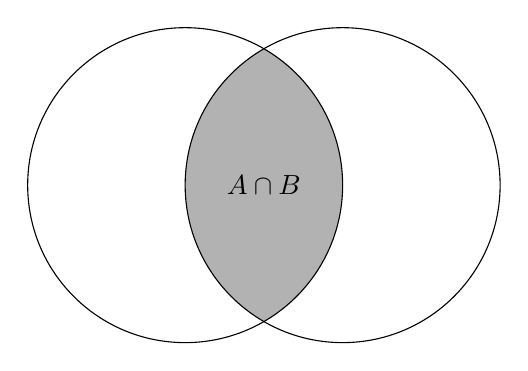
\begin{tikzpicture}
			\path[save path=\pathA](-1,0)circle(2cm);
			\path[save path=\pathB](1,0)circle(2cm);
			\begin{scope}
				\clip[use path=\pathA];
				\fill[black!30][use path=\pathB];
			\end{scope}
			\draw[use path=\pathA];
			\draw[use path=\pathB];
			\draw(0,0)node{\(A \cap B\)};
		\end{tikzpicture}
		\subcaption{集合的交}
	\end{subfigure}%
	\begin{subfigure}[b]{\subwidth}
		\centering
		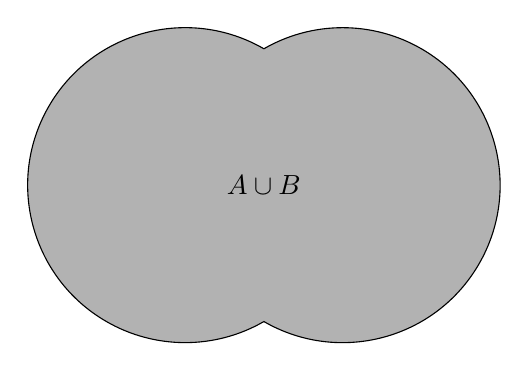
\begin{tikzpicture}
			\filldraw[fill=black!30,draw=black]
				(0,{sqrt(3)})arc[start angle=60,end angle=300,radius=2]
				arc[start angle=240,end angle=480,radius=2];
			\draw(0,0)node{\(A \cup B\)};
			\pgfresetboundingbox
			\path[use as bounding box] (-3,-2)rectangle(3,2);
		\end{tikzpicture}
		\subcaption{集合的并}
	\end{subfigure}%

	\begin{subfigure}[b]{\linewidth}
		\centering
		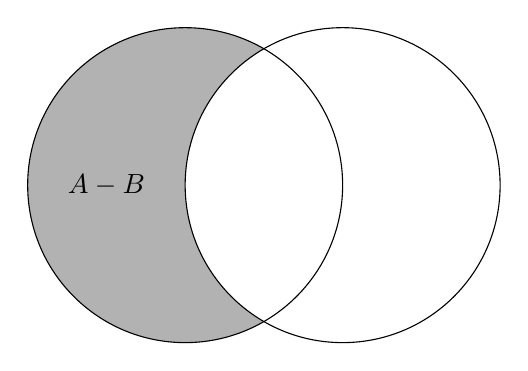
\begin{tikzpicture}
			\fill[black!30](0,{sqrt(3)})arc[start angle=60,end angle=300,radius=2]
				arc[start angle=240,end angle=120,radius=2];
			\draw(-1,0)circle(2cm);
			\draw(1,0)circle(2cm);
			\draw(-2,0)node{\(A-B\)};
			\pgfresetboundingbox
			\path[use as bounding box] (-3,-2)rectangle(3,2);
		\end{tikzpicture}
		\subcaption{集合的差}
	\end{subfigure}%
	\caption{韦恩图}
	\label{figure:集合论.韦恩图}
\end{figure}

\begin{property}
集合的运算满足以下性质:
\begin{enumerate}
\item 幂等律
\begin{gather}
	A \cap A = A, \\
	A \cup A = A.
\end{gather}

\item 交换律({\rm Commutative laws})
\begin{gather}
	A \cap B = B \cap A, \label{equation:集合论.集合代数公式1-1} \\
	A \cup B = B \cup A. \label{equation:集合论.集合代数公式1-2}
\end{gather}

\item 结合律({\rm Associative laws})
\begin{gather}
	(A \cap B) \cap C = A \cap (B \cap C), \label{equation:集合论.集合代数公式2-1} \\
	(A \cup B) \cup C = A \cup (B \cup C). \label{equation:集合论.集合代数公式2-2}
\end{gather}

\item 分配律({\rm Distributive laws})
\begin{gather}
	(A \cap B) \cup C = (A \cup C) \cap (B \cup C), \label{equation:集合论.集合代数公式3-1} \\
	(A \cup B) \cap C = (A \cap C) \cup (B \cap C), \label{equation:集合论.集合代数公式3-2} \\
	A \cup \bigcap \mathscr{B} = \bigcap\Set{A \cup X \given X \in \mathscr{B}}, \quad(\mathscr{B}\neq\emptyset) \label{equation:集合论.集合代数公式3-3} \\
	A \cap \bigcup \mathscr{B} = \bigcup\Set{A \cap X \given X \in \mathscr{B}}, \label{equation:集合论.集合代数公式3-4} \\
	\Powerset (A \cup B) \supseteq \Powerset A \cup \Powerset B, \label{equation:集合论.集合代数公式3-5} \\ %@see: 《Elements of Set Theory》 P26 Exercise 7(b).
	\Powerset (A \cap B) = \Powerset A \cap \Powerset B. \label{equation:集合论.集合代数公式3-6} %@see: 《Elements of Set Theory》 P26 Exercise 7(a)
\end{gather}

%@see: https://mathworld.wolfram.com/deMorgansLaws.html
\item 对偶律({\rm De Morgan's laws})(假设\(\mathscr{A}\neq\emptyset\))
\begin{gather}
	\Omega - (A \cap B)
	= (\Omega - A) \cup (\Omega - B), \label{equation:集合论.集合代数公式4-1} \\
	\Omega - (A \cup B)
	= (\Omega - A) \cap (\Omega - B), \label{equation:集合论.集合代数公式4-2} \\
	\Omega - \bigcup\mathscr{A}
	= \bigcap\Set{\Omega - X \given X\in\mathscr{A}}, \label{equation:集合论.集合代数公式4-3} \\
	\Omega - \bigcap\mathscr{A}
	= \bigcup\Set{\Omega - X \given X\in\mathscr{A}}. \label{equation:集合论.集合代数公式4-4}
\end{gather}

\item 与空集\(\emptyset\)和全集\(\Omega\)的运算(假设\(A \subseteq \Omega\))
\begin{gather}
	A \cup \emptyset = A, \label{equation:集合论.集合代数公式5-1} \\
	A \cap \emptyset = \emptyset, \label{equation:集合论.集合代数公式5-2} \\
	A \cup \Omega = \Omega, \label{equation:集合论.集合代数公式5-3} \\
	A \cap \Omega = A, \label{equation:集合论.集合代数公式5-4} \\
	A \cup (\Omega - A) = \Omega, \label{equation:集合论.集合代数公式5-5} \\
	A \cap (\Omega - A) = \emptyset, \label{equation:集合论.集合代数公式5-6} \\
	A \cup (A \cap B) = A, \\
	A \cap (A \cup B) = A, \\
	\Omega - \emptyset = \Omega, \\
	\Omega - \Omega = \emptyset, \\
	\Omega - (\Omega - A) = A.
\end{gather}

\item 包含关系
\begin{gather}
	A \subseteq B \implies A \cup C \subseteq B \cup C, \label{equation:集合论.集合代数公式6-1} \\
	A \subseteq B \implies A \cap C \subseteq B \cap C, \label{equation:集合论.集合代数公式6-2} \\
	A \subseteq B \implies \bigcup A \subseteq \bigcup B, \label{equation:集合论.集合代数公式6-3} \\
	A \subseteq B \implies (\Omega - B) \subseteq (\Omega - A), \label{equation:集合论.集合代数公式6-4} \\
	\emptyset \neq A \subseteq B \implies \bigcap B \subseteq \bigcap A, \label{equation:集合论.集合代数公式6-5} \\
	A \cap B \subseteq A, \\
	A \subseteq A \cup B.
\end{gather}

\item 差集
\begin{gather}
	A - B \subseteq A, \\
	B \subseteq \Omega
	\implies
	A - B = A \cap (\Omega - B), \\
	A \cup B = B
		\iff A \subseteq B
		\iff A \cap B = A
		\iff A - B = \emptyset, \label{equation:集合论.集合代数公式7-3} \\
	A \oplus B = B \oplus A, \\
	(A \oplus B) \oplus C = A \oplus (B \oplus C), \\
	A \oplus \emptyset = A, \\
	A \oplus A = \emptyset, \\
	A \oplus B = A \oplus C
		\iff B = C.
\end{gather}
\end{enumerate}
\begin{proof}
对\cref{equation:集合论.集合代数公式1-1} 证明如下:
\begin{align*}
	x \in A \cap B
	&\iff x \in A \land x \in B \\
	&\iff x \in B \land x \in A \\
	&\iff x \in B \cap A.
\end{align*}

对\cref{equation:集合论.集合代数公式1-2} 证明如下:
\begin{align*}
	x \in A \cup B
	&\iff x \in A \lor x \in B \\
	&\iff x \in B \lor x \in A \\
	&\iff x \in B \cup A.
\end{align*}

对\cref{equation:集合论.集合代数公式2-1} 证明如下:
\begin{align*}
	x \in (A \cap B) \cap C
	&\iff x \in A \cap B \land x \in C \\
	&\iff (x \in A \land x \in B) \land x \in C \\
	&\iff x \in A \land (x \in B \land x \in C) \\
	&\iff x \in A \land x \in B \cap C \\
	&\iff x \in A \cap (B \cap C).
\end{align*}

对\cref{equation:集合论.集合代数公式2-2} 证明如下:
\begin{align*}
	x \in (A \cup B) \cup C
	&\iff x \in A \cup B \lor x \in C \\
	&\iff (x \in A \lor x \in B) \lor x \in C \\
	&\iff x \in A \lor (x \in B \lor x \in C) \\
	&\iff x \in A \lor x \in B \cup C \\
	&\iff x \in A \cup (B \cup C).
\end{align*}

对\cref{equation:集合论.集合代数公式3-5} 证明如下:
\begin{align*}
	x \in \Powerset A \cup \Powerset B
	&\iff x \in \Powerset A \lor x \in \Powerset B \\
	&\iff x \subseteq A \lor x \subseteq B \\
	&\implies x \subseteq A \cup B \\
	&\iff x \in \Powerset (A \cup B),
\end{align*}
注意到中间步骤的\(\implies\)通常不是可逆的,
这是因为只要取\(a \subseteq A - B, b \subseteq B - A, x = a \cup b\),
就有\(x \subseteq A \cup B\)但是\(x \not\subseteq A \land x \not\subseteq B\),
因此\(x \subseteq A \cup B \notimplies x \subseteq A \lor x \subseteq B\).
%从上面的证明过程可以看出,
%要使\(\Powerset (A \cup B) = \Powerset A \cup \Powerset B\)成立,
%必有\[
%	\forall x \bigl(
%		x \subseteq A \cup B
%		\iff
%		x \subseteq A \lor x \subseteq B
%	\bigr)
%\]成立.
%取\(x = A \cup B\),
%由\(x \subseteq A \lor x \subseteq B\)
%可得\[
%	A \cup B = A \lor A \cup B = B.
%\]
%因此,当且仅当\(A \cup B \in \Set{A,B}\)时,
%就有\(\Powerset (A \cup B) = \Powerset A \cup \Powerset B\)成立.

对\cref{equation:集合论.集合代数公式3-6} 证明如下:
\begin{align*}
	x \in \Powerset (A \cap B)
	&\iff x \subseteq A \cap B \\
	&\iff x \subseteq A \land x \subseteq B \\
	&\iff x \in \Powerset A \land x \in \Powerset B \\
	&\iff x \in \Powerset A \cap \Powerset B.
\end{align*}

对\cref{equation:集合论.集合代数公式6-5} 证明如下:
\begin{align*}
	A \subseteq B
	&\iff (\forall t)[t \in A \implies t \in B] \\
	&\implies (\forall x)[
		(\forall b)[b \in B \implies x \in b]
		\implies
		(\forall a)[a \in A \implies x \in a]
	] \\
	&\iff (\forall x)[x \in \bigcap B \implies x \in \bigcap A].
	\qedhere
\end{align*}
\end{proof}
\end{property}

\begin{example}
%@see: 《Elements of Set Theory》 P32 Exercise 21.
设\(A,B\)是集合.
证明:\begin{equation}\label{equation:集合论.并集的并等于并的并集}
	\bigcup(A \cup B) = \bigcup A \cup \bigcup B.
\end{equation}
\begin{proof}
直接计算得
\begin{align*}
	x \in \bigcup(A \cup B)
	&\iff
	(\exists t)[t \in A \cup B \implies x \in t] \\
	&\iff
	(\exists t)[t \in A \lor t \in B \implies x \in t] \\
	&\iff
	(\exists t)[t \in A \implies x \in t] \lor (\exists t)[t \in B \implies x \in t] \\
	&\iff
	x \in \bigcup A \lor x \in \bigcup B \\
	&\iff
	x \in \bigcup A \cup \bigcup B.
	\qedhere
\end{align*}
\end{proof}
\end{example}

\begin{example}
%@see: 《Elements of Set Theory》 P32 Exercise 22.
设\(A,B\)是非空集合.
证明:\begin{equation}
	\bigcap(A \cup B) = \bigcap A \cap \bigcap B.
\end{equation}
%\begin{proof}
%直接计算得
%\begin{align*}
%	x \in \bigcap(A \cup B)
%	&\iff
%	x \in \bigcap A \land x \in \bigcap B \\
%	&\iff
%	x \in \bigcap A \cap \bigcap B.
%	\qedhere
%\end{align*}
%\end{proof}
\end{example}

\begin{example}
证明:\begin{equation}
	(A \cup B) - (A \cap B) = (A-B)\cup(B-A).
\end{equation}
\begin{proof}
根据集合交、并、差的定义,有
\begin{align*}
	x \in (A \cup B) - (A \cap B)
	&\iff x \in (A \cup B) \land x \notin (A \cap B) \\
	&\iff (x \in A \lor x \in B) \land \neg(x \in A \land x \in B) \\
	&\iff (x \in A \land \neg(x \in A \land x \in B))
	 \lor (x \in B \land \neg(x \in A \land x \in B)) \\
	&\iff (x \in A \land (x \notin A \lor x \notin B))
	 \lor (x \in B \land (x \notin A \lor x \notin B)) \\
	&\iff (x \in A \land x \notin B) \lor (x \in B \land x \notin A) \\
	&\iff x \in (A-B)\cup(B-A).
\qedhere
\end{align*}
\end{proof}
\end{example}

\input{集合论/集合论/关系}
\section{映射}
\subsection{映射的概念}
\begin{definition}
%@see: 《Elements of Set Theory》 P42 Definition
设\(F\)是关系,如果\[
	(\forall x \in \dom F)(\exists! y)[\opair{x,y} \in F],
\]
则称“关系\(F\)是一个\DefineConcept{映射}(function)”.
\end{definition}
可以从映射的定义中看出,虽然映射也是关系,
但映射有一般的关系所没有的特殊性质:
映射是\DefineConcept{单值的}(single-valued).
换句话说,对于关系\(F\),每个\(x\)可能对应若干个\(y\);
但是,对于映射\(F\),每个\(x\)就只对应一个\(y\).
我们可以把\(x\)与\(y\)这两个元素之间的对应关系记为\(x \mapsto y\).

我们把使得\(xFy\)成立的\(y\)称为“\(x\)(在映射\(F\)下)的\DefineConcept{像}%
(the \emph{value} of \(F\) at \(x\))”,
记为\(F(x)\),即\[
	y = f(x);
\]
称\(x\)为“\(y\)(在映射\(F\)下)的一个\DefineConcept{原像}”.
这里用的\(F(x)\)符号是欧拉提出的,
我们仅当\(F\)是一个映射且\(x\in\dom F\)时使用这个记号.
不过,我们也可以定义:\[
	F(x) \defeq \bigcup\Set{ y \given \opair{x,y} \in F }.
\]
它对于任意\(F\)和\(x\)都有意义.

映射是如此重要,以至于各家对用于描述映射的术语没有达成统一.
以下是两种最常采用的术语.

设\(X,Y\)都是集合,
如果\(f\)是一个映射,且\(\dom f = X\),\(\ran f \subseteq Y\),
则称“\(f\)是从\(X\)到\(Y\)的\DefineConcept{映射}%
(\(f\) is a function \emph{from} \(X\) \emph{into} \(Y\))”,
或称“\(f\)将\(X\)映射到\(Y\)里%
(\(f\) \emph{maps} \(X\) \emph{into} \(Y\))”,
记作\[
	f\colon X \to Y.
\]
如果还有\(\ran f = Y\),
那么称“\(f\)是从\(X\)到\(Y\)上的映射%
(\(f\) is a function from \(X\) \emph{onto} \(Y\))”,
或称“\(f\)将\(X\)映射到\(Y\)上%
(\(f\) \emph{maps} \(X\) \emph{onto} \(Y\))”,
或称“\(f\)是\DefineConcept{满射}(surjective)”.
我们可以说“任意映射总将它的定义域映射到它的值域上”,
还可以说“任意映射总把它的定义域映射到以它的值域为子集的任意集合\(B\)里”.
注意到两种说法的区别,“上”字和“里”字的选用,
不光取决于映射\(f\)本身,还取决于我们讨论的集合\(B\).

如果\[
	(\forall y \in \ran f)
	(\exists! x)
	[\opair{x,y} \in f],
\]
那么称“映射\(f\)是\DefineConcept{一对一的}(one-to-one)”.

有时候我们希望把“一对一的”这个概念套用到一般的关系上,
它们往往不是映射,因此我们类比于“单值的”,创造出“单根的”这个概念.
\begin{definition}
%@see: 《Elements of Set Theory》 P43 Definition
如果集合\(R\)满足\[
	(\forall y \in \ran R)
	(\exists! x)
	[\opair{x,y} \in R],
\]
则称“\(R\)是\DefineConcept{单根的}(single-rooted)”.
\end{definition}

因此,我们可以说,“一个映射是单根的”当且仅当“这个映射是一对一的”.

如果\[
	(\forall x_1, x_2 \in \dom f)
	[x_1 \neq x_2 \implies f(x_1) \neq f(x_2)],
\]
那么称“\(f\)是\DefineConcept{单射}(injective)”.

由于映射本就是单值的,若它还是单根的,那么这个映射就是单射.
换句话说,“一对一的映射”和“单射”是相同的概念.

如果\(f\)既是单射,又是满射,
那么称“\(f\)是\DefineConcept{双射}(bijective)
或\DefineConcept{一一映射}”.

我们可以给出一个最平凡的一一映射.
\begin{definition}
设\(X\)是集合.
我们把\[
	\Set{ \opair{x,x} \given x \in X }
\]称为“(\(X\)上的)\DefineConcept{恒等映射}或\DefineConcept{恒同映射}”,
常记为\(i_X\).
\end{definition}

\begin{example}
%@see: 《Elements of Set Theory》 P52 Exercise 11
设\(F,G\)都是映射,
\(\dom F = \dom G = X\),且\[
	(\forall x \in X)[F(x) = G(x)].
\]
证明:\(F=G\).
\begin{proof}
显然有
\begin{align*}
	F=G
	&\iff (\forall x \in X)(\exists!y)[
		\opair{x,y} \in F
		\iff
		\opair{x,y} \in G
	] \\
	&\iff (\forall x \in X)(\exists!y)[
		y = F(x) = G(x)
	] \\
	&\iff (\forall x \in X)[F(x) = G(x)].
	\qedhere
\end{align*}
\end{proof}
\end{example}

\begin{example}
%@see: 《Elements of Set Theory》 P52 Exercise 12
设\(f,g\)都是映射.
证明:\[
	f \subseteq g
	\iff
	\dom f \subseteq \dom g
	\land
	(\forall x \in \dom f)
	[f(x) = g(x)].
\]
\begin{proof}
直接有
\begin{align*}
	f \subseteq g
	&\iff (\forall x)(\exists!y)[\opair{x,y} \in f \implies \opair{x,y} \in g] \\
	&\iff (\forall x \in \dom f)[x \in \dom g]\land(\forall x \in \dom f)(\exists!y)[y=f(x)=g(x)] \\
	&\iff [\dom f \subseteq \dom g]\land(\forall x \in \dom f)[f(x)=g(x)].
	\qedhere
\end{align*}
\end{proof}
\end{example}

\begin{example}
%@see: 《Elements of Set Theory》 P53 Exercise 13
设\(f,g\)都是映射,\(f \subseteq g\)且\(\dom g \subseteq \dom f\).
证明:\(f=g\).
%TODO
\end{example}

\begin{example}
%@see: 《Elements of Set Theory》 P53 Exercise 14
设\(f,g\)都是映射.
证明:
\begin{enumerate}
	\item \(f \cap g\)是映射.
	\item \(f \cup g\)是映射的充分必要条件是\[
		(\forall x \in (\dom f)\cap(\dom g))[f(x)=g(x)].
	\]
\end{enumerate}
%TODO
\end{example}

\begin{example}
%@see: 《Elements of Set Theory》 P53 Exercise 15
\def\A{\mathscr{A}}%
设\(\A\)是一组映射,且\[
	(\forall f,g\in\A)[f \subseteq g \lor g \subseteq f].
\]
证明:\(\bigcup\A\)也是映射.
%TODO
\end{example}

\begin{example}
%@see: 《Elements of Set Theory》 P53 Exercise 16
证明:不存在一个集合,使得每个映射都属于它.
%TODO
\end{example}

\begin{example}
%@see: 《实变函数论》(周民强) P14 思考题5.
设\(f\colon X \to Y,
g\colon Y \to X\).
证明:若\[
	(\forall x \in X)[g(f(x)) = x],
\]
则\(f\)是单射,\(g\)是满射.
%TODO
\end{example}

\subsection{逆,复合,限制,像,原像}
以下定义的操作通常用在映射上,有时候也用于关系,但也可以用于任意集合.
\begin{definition}
设\(A,F,G\)都是集合.
\begin{enumerate}
	\item 称集合\[
		\Set*{ \opair{u,v} \given \opair{v,u} \in F }
	\]为“\(F\)的\DefineConcept{逆}%
	(the \emph{inverse} of \(F\))”,
	记作\(F^{-1}\).

	特别地,如果\(F^{-1}\)是映射,
	则称“\(F^{-1}\)是\(F\)的\DefineConcept{逆映射}”.

	\item 称集合\[
		\Set*{ \opair{u,v} \given (\exists t)[\opair{u,t} \in G \land \opair{t,v} \in F] }
	\]为“\(F\)和\(G\)的\DefineConcept{复合}%
	(the \emph{composition} of \(F\) and \(G\))”,
	记作\(F \circ G\).

	\item 称集合\[
		\Set*{ \opair{u,v} \given \opair{u,v} \in F \land u \in A }
	\]为“\(F\)在\(A\)上的\DefineConcept{限制}%
	(the \emph{restriction} of \(F\) to \(A\))”,
	记作\(F \upharpoonright A\).

	\item 称集合\[
		\Set*{ v \given (\exists u \in A)[\opair{u,v} \in F] }
	\]为“\(A\)在\(F\)下的\DefineConcept{像}%
	(the \emph{image} of \(A\) \emph{under} \(F\))”,
	记作\(F\ImageOfSetUnderRelation{A}\).
\end{enumerate}
\end{definition}

当\(F\)是一个映射,且\(A \subseteq \dom F\)时,
\(F\ImageOfSetUnderRelation{A}\)这个概念可能更容易理解,
因为这时候\[
	F\ImageOfSetUnderRelation{A}
	= \Set{ F(u) \given u \in A }.
\]

我们可以利用子集公理构造出上述定义下的所需集合的存在性.
特别地,\[
	F^{-1} \subseteq \ran F \times \dom F, \qquad
	F \circ G \subseteq \dom G \times \ran F,
\]\[
	F \upharpoonright A \subseteq F, \qquad
	F\ImageOfSetUnderRelation{A} \subseteq \ran F.
\]

例如,我们可以按如下方法正当化“关系\(F\)的逆”的定义:
根据子集公理,存在集合\(B\),使得对于任意\(x\),总有\begin{align*}
	x \in B
	&\iff
	[x \in \ran F \times \dom F]
	\land
	(\exists u)(\exists v)[x = \opair{u,v} \land \opair{v,u} \in F], \\
	&\iff
	(\exists u)(\exists v)[x = \opair{u,v} \land \opair{v,u} \in F].
\end{align*}
再根据外延公理,可以保证集合\(B\)的唯一性.
因此我们可以将集合\(B\)记为\(F^{-1}\).

\begin{definition}
%@see: 《点集拓扑讲义(第四版)》(熊金城) P22 定义1.5.4
设\(A,B,X\)都是集合,\(A \subset B\).
若映射\(F\colon A \to X\)和\(G\colon B \to X\)满足\(F \subset G\),
则称“\(G\)是\(F\)在\(B\)上的\DefineConcept{扩张}”.
\end{definition}

\begin{theorem}
\(F \upharpoonright \emptyset = \emptyset\).
\end{theorem}

\begin{theorem}
\(F\ImageOfSetUnderRelation{A} = \ran(F \upharpoonright A)\).
\begin{proof}
根据值域的定义有\begin{align*}
	v \in \ran(F \upharpoonright A)
	&\iff
	(\exists u)[\opair{u,v} \in F \upharpoonright A] \\
	&\iff
	(\exists u)[\opair{u,v} \in F \land u \in A] \\
	&\iff
	v \in F\ImageOfSetUnderRelation{A}.
	\qedhere
\end{align*}
\end{proof}
\end{theorem}

\begin{definition}
设\(F\)是关系,\(A\)是集合,那么称集合\[
	\Set*{ x \in \dom F \given F(x) \in A }
\]为“集合\(A\)在关系\(F\)下的\DefineConcept{原像}%
(the \emph{inverse image} of \(A\) under \(F\))”,
记作\(F^{-1}\ImageOfSetUnderRelation{A}\).
\end{definition}

一般来说,一个映射的逆不一定是映射.
例如,\(F=\Set{ \opair{1,1},\opair{2,1} }\)是一个映射,
但它的逆\(F^{-1}=\Set{ \opair{1,1},\opair{1,2} }\)不是映射.

\begin{theorem}\label{theorem:集合论.关系的逆的定义域值域以及关系的二重逆}
%@see: 《Elements of Set Theory》 P46 Theorem 3E
设\(F\)是集合,则有\begin{gather}
	\dom F^{-1} = \ran F, \\
	\ran F^{-1} = \dom F.
\end{gather}

如果\(F\)是关系,则有\begin{equation}
	(F^{-1})^{-1} = F.
\end{equation}
\begin{proof}
因为\[
	y \in \dom F^{-1}
	\iff
	(\exists x)[yF^{-1}x]
	\iff
	(\exists x)[xFy]
	\iff
	y \in \ran F,
\]
所以\(\dom F^{-1} = \ran F\).

因为\[
	x \in \ran F^{-1}
	\iff
	(\exists y)[yF^{-1}x]
	\iff
	(\exists y)[xFy]
	\iff
	x \in \dom F,
\]
所以\(\ran F^{-1} = \dom F\).

因为\[
	\opair{x,y} \in (F^{-1})^{-1}
	\iff
	\opair{y,x} \in F^{-1}
	\iff
	\opair{x,y} \in F,
\]
所以\((F^{-1})^{-1} = F\).
\end{proof}
\end{theorem}

\begin{theorem}\label{theorem:集合论.关系及其逆是映射的充分必要条件}
%@see: 《Elements of Set Theory》 P46 Theorem 3F
设\(F\)是集合,则“\(F^{-1}\)是映射”的充分必要条件是:\(F\)是单根的.

设\(F\)是关系,则“\(F\)是映射”的充分必要条件是:\(F^{-1}\)是单根的.
\begin{proof}
容易看出\begin{align*}
	\text{\(F^{-1}\)是映射}
	&\iff
	\text{\(F^{-1}\)是单值的} \\
	&\iff
	(\forall x \in \dom F^{-1})(\exists! y)[xF^{-1}y] \\
	&\iff
	(\forall x \in \ran F)(\exists! y)[yFx] \\
	&\iff
	\text{\(F\)是单根的}, \\
	\text{\(F\)是映射}
	&\iff
	\text{\(F\)是单值的} \\
	&\iff
	(\forall x \in \dom F)(\exists! y)[xFy] \\
	&\iff
	(\forall x \in \ran F^{-1})(\exists! y)[yF^{-1}x] \\
	&\iff
	\text{\(F^{-1}\)是单根的}.
	\qedhere
\end{align*}
\end{proof}
\end{theorem}

\begin{theorem}\label{theorem:集合论.逆映射的计算}
%@see: 《Elements of Set Theory》 P46 Theorem 3G
设\(F\)是单射.
\begin{enumerate}
	\item 如果\(x \in \dom F\),那么\[
		F^{-1}(F(x)) = x.
	\]

	\item 如果\(y \in \ran F\),那么\[
		F(F^{-1}(y)) = y.
	\]
\end{enumerate}
\begin{proof}
假设\(x \in \dom F\),
那么\(\opair{x,F(x)} \in F\),且\(\opair{F(x),x} \in F^{-1}\),
于是\(F(x) \in \dom F^{-1}\).
因为\(F\)是单射,是单根的,
所以由\cref{theorem:集合论.关系及其逆是映射的充分必要条件}
可知\(F^{-1}\)是映射,
从而\(x = F^{-1}(F(x))\).

如果\(y \in \ran F\),
那么根据本定理第1条,以及\((F^{-1})^{-1} = F\),可知\[
	F(F^{-1}(y)) = (F^{-1})^{-1}(F^{-1}(y)) = y.
	\qedhere
\]
\end{proof}
\end{theorem}

\begin{theorem}\label{theorem:集合论.映射的复合也是映射}
%@see: 《Elements of Set Theory》 P47 Theorem 3H
设\(F,G\)都是映射,则\(F \circ G\)是映射,且\[
	\dom(F \circ G)
	= \Set*{ x \in \dom G \given G(x) \in \dom F },
\]\[
	(\forall x \in \dom(F \circ G))
	[(F \circ G)(x) = F(G(x))].
\]
\begin{proof}
要证\(F \circ G\)是一个映射,
假设有\(\opair{x,y} \in F \circ G\)和\(\opair{x,z} \in F \circ G\)同时成立.
那么,\[
	(\exists p)[\opair{x,p} \in G \land \opair{p,y} \in F]
	\quad\text{和}\quad
	(\exists q)[\opair{x,q} \in G \land \opair{q,z} \in F]
\]同时成立.
既然\(G\)是映射,必有\(p = q\).
同理,\(F\)是映射,必有\(y = z\).
因此\(F \circ G\)是映射.

现在再假设\(x \in \dom G\)且\(G(x) \in \dom F\).
我们必须证明\[
	x \in \dom(F \circ G)
	\quad\text{和}\quad
	(F \circ G)(x) = F(G(x)).
\]
我们知道\[
	\opair{x,G(x)} \in G,
	\qquad
	\opair{G(x),F(G(x))} \in F.
\]
因此\(\opair{x,F(G(x))} \in F \circ G\).

反过来说,如果\(x \in \dom(F \circ G)\),
那么就有\[
	(\exists y)(\exists t)
	[\opair{x,t} \in G \land \opair{t,y} \in F].
\]
于是就有\(x \in \dom G\)和\(t = G(x) \in \dom F\).
\end{proof}
\end{theorem}

容易看出,映射的复合是有顺序的,
\(f \circ g\)有意义并不代表\(g \circ f\)也有意义.
即便两者都有意义,它们也未必相同.

\begin{example}
%@see: 《Elements of Set Theory》 P47 Example
假设\(G\)是单射,
那么,根据\cref{theorem:集合论.映射的复合也是映射},
\(G^{-1} \circ G\)也是一个映射,
它的定义域为\[
	\Set{ x \in \dom G \given G(x) \in \dom G^{-1} }
	= \dom G,
\]
并且,对于\(\forall x \in \dom(G^{-1} \circ G)\),
有\begin{align*}
	(G^{-1} \circ G)(x) &= G^{-1}(G(x)) \\
	&= x. \tag{\cref{theorem:集合论.逆映射的计算}}
\end{align*}
因此,\(G^{-1} \circ G\)就是\(I_{\dom G}\),
\(\dom G\)上的恒等映射.
同理,\(G \circ G^{-1}\)是\(I_{\ran G}\),
\(\ran G\)上的恒等映射.
\end{example}

\begin{theorem}
%@see: 《Elements of Set Theory》 P65 Exercise 53.
设\(R,S\)是集合,那么\begin{gather}
	(R \cup S)^{-1} = R^{-1} \cup S^{-1},
	\label{equation:集合论.并的逆等于逆的并} \\
	(R \cap S)^{-1} = R^{-1} \cap S^{-1},
	\label{equation:集合论.交的逆等于逆的交} \\
	(R - S)^{-1} = R^{-1} - S^{-1}.
	\label{equation:集合论.差的逆等于逆的差}
\end{gather}
\begin{proof}
对\cref{equation:集合论.并的逆等于逆的并} 证明如下:
\begin{align*}
	\opair{x,y} \in (R \cup S)^{-1}
	&\iff \opair{y,x} \in R \cup S \\
	&\iff \opair{y,x} \in R \lor \opair{y,x} \in S \\
	&\iff \opair{x,y} \in R^{-1} \lor \opair{x,y} \in S^{-1} \\
	&\iff \opair{x,y} \in R^{-1} \cup S^{-1}.
\end{align*}

对\cref{equation:集合论.交的逆等于逆的交} 证明如下:
\begin{align*}
	\opair{x,y} \in (R \cap S)^{-1}
	&\iff \opair{y,x} \in R \cap S \\
	&\iff \opair{y,x} \in R \land \opair{y,x} \in S \\
	&\iff \opair{x,y} \in R^{-1} \land \opair{x,y} \in S^{-1} \\
	&\iff \opair{x,y} \in R^{-1} \cap S^{-1}.
\end{align*}

对\cref{equation:集合论.差的逆等于逆的差} 证明如下:
\begin{align*}
	\opair{x,y} \in (R - S)^{-1}
	&\iff \opair{y,x} \in R - S \\
	&\iff \opair{y,x} \in R \land \opair{y,x} \notin S \\
	&\iff \opair{x,y} \in R^{-1} \land \opair{x,y} \notin S^{-1} \\
	&\iff \opair{x,y} \in R^{-1} - S^{-1}.
	\qedhere
\end{align*}
\end{proof}
\end{theorem}

\begin{theorem}\label{theorem:集合论.复合的逆}
%@see: 《Elements of Set Theory》 P47 Theorem 3I
设\(F,G\)都是集合,那么\[
	(F \circ G)^{-1} = G^{-1} \circ F^{-1}.
\]
\begin{proof}
易知\((F \circ G)^{-1}\)和\(G^{-1} \circ F^{-1}\)都是关系,且\begin{align*}
	\opair{x,y} \in (F \circ G)^{-1}
	&\iff
	\opair{y,x} \in F \circ G \\
	&\iff
	(\exists t)[\opair{y,t} \in G \land \opair{t,x} \in F] \\
	&\iff
	(\exists t)[\opair{x,t} \in F^{-1} \land \opair{t,y} \in G^{-1}] \\
	&\iff
	\opair{x,y} \in G^{-1} \circ F^{-1}.
	\qedhere
\end{align*}
\end{proof}
\end{theorem}

由\cref{theorem:集合论.复合的逆} 立即可得如下推论.
\begin{proposition}\label{theorem:集合论.复合的逆.推论1}
设\(F\)是集合,那么\[
	(F^{-1} \circ F)^{-1} = F^{-1} \circ F.
\]
\end{proposition}

\begin{axiom}[选择公理(第一种形式)]
对于任意关系\(R\),存在映射\(H\),满足\[
	H \subseteq R,
	\quad\text{且}\quad
	\dom H = \dom R.
\]
\end{axiom}

\begin{theorem}
%@see: 《Elements of Set Theory》 P48 Theorem 3J
设映射\(F\colon A \to B\),其中\(A\)是非空集合.
\begin{enumerate}
	\item “存在映射\(G\colon B \to A\)(称其为\DefineConcept{左逆}),
	使得\(G \circ F\)是\(A\)上的恒等映射\(I_A\)”是“\(F\)是单射”的充分必要条件.

	\item “存在映射\(H\colon B \to A\)(称其为\DefineConcept{右逆}),
	使得\(F \circ H\)是\(B\)上的恒等映射\(I_B\)”是“\(F\)是满射”的充分必要条件.
\end{enumerate}
\begin{proof}
\begin{enumerate}
	\item
	先证充分性.
	我们假设存在映射\(G\)使得\(G \circ F = I_A\).
	如果\(F(x) = F(y)\),那么\[
		x = G(F(x)) = G(F(y)) = y,
	\]
	于是\(F\)是单射.

	再证必要性.
	假设\(F\)是单射,
	那么根据\cref{theorem:集合论.关系的逆的定义域值域以及关系的二重逆,theorem:集合论.关系及其逆是映射的充分必要条件},
	\(F^{-1}\)是一个从\(\ran F\)到\(A\)上的映射.
	现在我们需要将\(F^{-1}\)延拓为以\(B\)为定义域的映射\(G\).
	因为\(A\)是非空集合,
	于是我们可以取定\(a \in A\),
	然后令\[
		G(x) = \left\{ \begin{array}{ll}
			F^{-1}(x), & x \in \ran F, \\
			a, & x \in B - \ran F,
		\end{array} \right.
	\]或者令\[
		G = F^{-1} \cup (B - \ran F) \times \Set{a}.
	\]
	这个构造出来的映射\(G\)是一个从\(B\)到\(A\)里的映射,
	且满足\[
		\dom(G \circ F) = A,
	\]
	以及\[
		(\forall x \in A)[G(F(x)) = F^{-1}(F(x)) = x],
	\]
	于是\(G \circ F = I_A\)成立.

	\item
	我们还是先证充分性.
	假设存在映射\(H\)使得\(F \circ H = I_B\).
	那么\[
		(\forall y \in B)[y = F(H(y))],
	\]
	从而\(y \in \ran F\),
	于是\(\ran F = B\).

	必要性的证明稍显困难.
	我们不能直接取\(H = F^{-1}\),
	因为一般而言\(F\)不会是单射,
	\(F^{-1}\)也不会是一个映射.
	假设\(F\)将\(A\)映射到\(B\)上,\(\ran F = B\).
	现在我们需要为每个\(y \in B\)选择某个\(x\),使得\(F(x) = y\),然后令\(H(y) = x\);
	考虑到\(y \in \ran F\),这样的\(x\)必定存在.
	虽然我们知道对于每个\(y\),存在一个合适的\(x\),
	但是我们无法据此构造所求映射\(H\).
	因此,我们需要引入选择公理.
	借助选择公理,我们可以令映射\(H\)满足\(H \subseteq F^{-1}\)且\(\dom H = \dom F^{-1} = B\).
	于是\(H\)满足\[
		(\forall y \in B)
		[
			\opair{y,H(y)} \in F^{-1}
			\iff
			\opair{H(y),y} \in F
			\iff
			F(H(y)) = y
		].
		\qedhere
	\]
\end{enumerate}
\end{proof}
\end{theorem}

\begin{theorem}
%@see: 《Elements of Set Theory》 P48 Theorem 3K
设\(A,B,F\)都是集合.
\def\F#1{F\ImageOfSetUnderRelation{#1}}
\begin{enumerate}
	\item 并的像是像的并:\begin{gather}
		\F{A \cup B}
		= \F{A} \cup \F{B},
		\label{equation:集合论.并的像与像的并的关系1} \\
		\F{\bigcup A}
		= \bigcup\Set{ \F{a} \given a \in A }.
		\label{equation:集合论.并的像与像的并的关系2}
	\end{gather}

	\item 交的像包含于像的交:\begin{gather}
		\F{A \cap B}
		\subseteq \F{A} \cap \F{B},
		\label{equation:集合论.交的像与像的交的关系1} \\
		\F{\bigcap A}
		\subseteq \bigcap\Set{ \F{a} \given a \in A }.
		\label{equation:集合论.交的像与像的交的关系2}
		\quad(A \neq \emptyset)
	\end{gather}
	若\(F\)是单根的,则以上两式取“=”号.

	\item 差的像包含像的差:\begin{equation}
		\F{A} - \F{B}
		\subseteq \F{A-B}.
		\label{equation:集合论.差的像与像的差的关系}
	\end{equation}
	若\(F\)是单根的,则上式取“=”号.
\end{enumerate}
\begin{proof}
\cref{equation:集合论.并的像与像的并的关系1} 证明如下:
\begin{align*}
	y \in \F{A \cup B}
	&\iff (\exists x \in A \cup B)[\opair{x,y} \in F] \\
	&\iff (\exists x \in A)[\opair{x,y} \in F]
			\lor (\exists x \in B)[\opair{x,y} \in F] \\
	&\iff y \in \F{A} \lor y \in \F{B}.
\end{align*}

\cref{equation:集合论.交的像与像的交的关系1} 证明如下:
\begin{align*}
	y \in \F{A \cap B}
	&\iff (\exists x \in A \cap B)[\opair{x,y} \in F] \\
	&\implies (\exists x \in A)[\opair{x,y} \in F]
		\land (\exists x \in B)[\opair{x,y} \in F] \\
	&\iff y \in \F{A} \land y \in \F{B}.
\end{align*}
注意到中间步骤的\(\implies\)不总是可逆的,
这时因为虽然有\[
	(\exists x_1 \in A)[\opair{x_1,y} \in F], \qquad
	(\exists x_2 \in B)[\opair{x_2,y} \in F],
\]
但是可能\[
	(\forall x \in A \cap B)[\opair{x,y} \notin F].
\]
不过,如果\(F\)是单根的,那么必有\(x_1 = x_2 \in A \cap B\),
这时候中间步骤的\(\implies\)是可逆的,可以改为\(\iff\).

\cref{equation:集合论.并的像与像的并的关系2,equation:集合论.交的像与像的交的关系2} 分别是%
\cref{equation:集合论.并的像与像的并的关系1,equation:集合论.交的像与像的交的关系1} 的简单推广,
故略去证明.

\cref{equation:集合论.差的像与像的差的关系} 证明如下:
\begin{align*}
	y \in \F{A} - \F{B}
	&\iff (\exists x \in A)[\opair{x,y} \in F]
		\land \neg[(\exists t \in B)[\opair{t,y} \in F]] \\
	&\implies (\exists x \in A - B)[\opair{x,y} \in F] \\
	&\iff y \in \F{A - B}.
\end{align*}
若\(F\)是单根的,则\[
	(\exists! x)[\opair{x,y} \in F].
\]
这种情况下,中间步骤的\(\implies\)可以改为\(\iff\).
\end{proof}
\end{theorem}

\begin{corollary}
%@see: 《Elements of Set Theory》 P48 Corollary 3L
设\(G\)是映射,\(A,B\)都是集合.
\def\G#1{G^{-1}\ImageOfSetUnderRelation{#1}}
\begin{gather}
	\G{\bigcup A} = \bigcup\Set*{ \G{a} \given a \in A },
	\label{equation:集合论.并的原像与原像的并的关系} \\
	\G{\bigcap A} = \bigcap\Set*{ \G{a} \given a \in A }, \quad A \neq \emptyset,
	\label{equation:集合论.交的原像与原像的交的关系} \\
	\G{A - B} = \G{A} - \G{B}.
	\label{equation:集合论.差的原像与原像的差的关系}
\end{gather}
\end{corollary}

\begin{example}
%@see: 《Elements of Set Theory》 P53 Exercise 22.(a)
\def\F#1{F\ImageOfSetUnderRelation{#1}}
证明:\begin{equation}
	A \subseteq B \implies \F{A} \subseteq \F{B}.
\end{equation}
\begin{proof}
因为\(A \subseteq B\),所以\(A \cap B = A\),
那么由\cref{equation:集合论.交的像与像的交的关系1} 可知,\[
	\F{A} = \F{A \cap B} \subseteq \F{A} \cap \F{B} \subseteq \F{B}.
	\qedhere
\]
\end{proof}
\end{example}

\begin{example}
%@see: 《Elements of Set Theory》 P53 Exercise 22.(b)
证明:\begin{equation}
	(F \circ G)\ImageOfSetUnderRelation{A}
	= F\ImageOfSetUnderRelation{G\ImageOfSetUnderRelation{A}}.
\end{equation}
%TODO
\end{example}

\begin{example}
%@see: 《Elements of Set Theory》 P53 Exercise 22.(c)
证明:\begin{equation}
	Q \upharpoonright (A \cup B)
	= (Q \upharpoonright A)\cup(Q \upharpoonright B).
\end{equation}
%TODO
\end{example}

\begin{example}
%@see: 《Elements of Set Theory》 P65 Exercise 59.
设\(A,B,Q\)是集合.
证明:\begin{gather}
	Q \upharpoonright (A \cap B)
	= (Q \upharpoonright A) \cap (Q \upharpoonright B), \\
	Q \upharpoonright (A - B)
	= (Q \upharpoonright A)
	- (Q \upharpoonright B).
\end{gather}
%TODO
\end{example}

\begin{example}
%@see: 《Elements of Set Theory》 P65 Exercise 60.
设\(A,R,S\)是集合.
证明:\begin{equation}
	(R \circ S) \upharpoonright A = R \circ (S \upharpoonright A).
\end{equation}
%TODO
\end{example}

\begin{proposition}\label{theorem:集合论.与逆相等的充分必要条件}
设\(R\)是集合,
则\(R^{-1} \subseteq R
\iff R^{-1} = R
\iff R \subseteq R^{-1}\).
\begin{proof}
容易看出\begin{align*}
	R^{-1} \subseteq R
	&\iff
	(\forall x)(\forall y)[xR^{-1}y \implies xRy] \\
	&\iff
	(\forall x)(\forall y)[yRx \implies xRy] \\
	&\iff
	(\forall u)(\forall v)[uRv \implies vRu] \\
	&\iff
	(\forall u)(\forall v)[uRv \implies uR^{-1}v] \\
	&\iff
	R \subseteq R^{-1},
\end{align*}
再由\(R^{-1} \subseteq R \land R \subseteq R^{-1}\)
便得\(R = R^{-1}\).
\end{proof}
\end{proposition}

\subsection{有标集族,指标集}\label{section:集合论.指标集}
%@see: https://math.libretexts.org/Bookshelves/Mathematical_Logic_and_Proof/Book%3A_Mathematical_Reasoning__Writing_and_Proof_(Sundstrom)/05%3A_Set_Theory/5.05%3A_Indexed_Families_of_Sets
\begin{definition}
%@see: 《Elements of Set Theory》 P51
设\(F\)是映射,\(I\)是集合,\(\dom F \supseteq I\).

对于\(\forall i \in I\),
把\(i\)在映射\(F\)下的像\(F(i)\)记作\(F_i\),
即\[
	F_i \defeq F(i).
\]

把\(F\)在\(I\)上的限制\(F \upharpoonright I\)
称为“一个以\(I\)为指标集的\DefineConcept{有标集族}(an \emph{indexed family of sets} indexed by \(I\))”,
记作\(\{F_i\}_{i \in I}\),
即\[
	\{F_i\}_{i\in I}
	\defeq
	F \upharpoonright I.
\]
把\(I\)的每一个元素称为一个\DefineConcept{指标}(index).
把\(I\)称为“\(\{F_i\}_{i \in I}\)的\DefineConcept{指标集}(indexing set)”.
\end{definition}

\begin{example}
当我们谈到有标集族\(\{R\}_{i \in I}\)时,
我们指的就是映射\(F = I \times \{R\}\),
即对于每一个\(i \in I\)都指定同一个集合\(F(i) = R\).
\end{example}

\begin{example}
设\(\mathscr{A}\)是一个集族,
那么恒同映射\(\{A\}_{A \in \mathscr{A}} = \Set{ \opair{A,A} \given A \in \mathscr{A} }\)
就是一个以\(\mathscr{A}\)为指标集的有标集族.
有时候我们会把\(\{A\}_{A \in \mathscr{A}}\)简记为“有标集族\(\mathscr{A}\)”.
\end{example}

\begin{definition}
%@see: 《Elements of Set Theory》 P51
%@see: 《点集拓扑讲义(第四版)》(熊金城) P26 定义1.6.1
设有标集族\(\{F_i\}_{i \in I}\).

定义:\begin{equation}
	\bigcup_{i \in I} F_i
	\defeq
	\bigcup\Set{ F_i \given i \in I },
\end{equation}
把它称为“有标集族\(\{F_i\}_{i \in I}\)的并”.

当指标集\(I\)非空时,定义:
\begin{equation}
	\bigcap_{i \in I} F_i
	\defeq
	\bigcap\Set{ F_i \given i \in I },
\end{equation}
把它称为“有标集族\(\{F_i\}_{i \in I}\)的交”.
\end{definition}
应该注意到:
\(\bigcup_{i \in \emptyset} F_i = \emptyset\),
而\(\bigcap_{i \in \emptyset} F_i\)没有定义.

\begin{theorem}
%@see: 《点集拓扑讲义(第四版)》(熊金城) P26 定理1.6.1
设\(\{A_i\}_{i \in I}\)和\(\{B_j\}_{j \in J}\)是两个非空有标集族.
如果\[
	\Set{ A_i \given i \in I }
	= \Set{ B_j \given j \in J },
\]
则有\begin{gather}
	\bigcup_{i \in I} A_i = \bigcup_{j \in J} B_j, \\
	\bigcap_{i \in I} A_i = \bigcap_{j \in J} B_j.
\end{gather}
%TODO
\end{theorem}

\begin{theorem}
%@see: 《点集拓扑讲义(第四版)》(熊金城) P27 定理1.6.2
设\(\{A_i\}_{i \in I}\)是一个非空有标集族,
\(B\)是一个集合,
则\begin{itemize}
	\item 对于任意\(i_0 \in I\),有\[
		\bigcap_{i \in I} A_i \subseteq A_{i_0} \subseteq \bigcup_{i \in I} A_i;
	\]

	\item {\rm 分配律}\begin{gather*}
		B \cap \left( \bigcup_{i \in I} A_i \right)
		= \bigcup_{i \in I} \left( B \cap A_i \right), \\
		B \cup \left( \bigcap_{i \in I} A_i \right)
		= \bigcap_{i \in I} \left( B \cup A_i \right);
	\end{gather*}

	\item {\rm 对偶律}\begin{gather*}
		B - \left( \bigcup_{i \in I} A_i \right)
		= \bigcap_{i \in I} \left( B - A_i \right), \\
		B - \left( \bigcap_{i \in I} A_i \right)
		= \bigcup_{i \in I} \left( B - A_i \right).
	\end{gather*}
\end{itemize}
%TODO
\end{theorem}

\subsection{映射空间}
对于任意给定的集合\(A,X\),定义:\[
	X^A \defeq \Set{ F \given F\ \text{是从\(A\)到\(X\)的映射} }.
\]
我们把\(X^A\)称为“从\(A\)到\(X\)的\DefineConcept{映射空间}”.

因为\(F\colon A \to X\)必有\(F \subseteq A \times X\),\(F \in \Powerset(A \times X)\),
所以我们可以对集合\(\Powerset(A \times X)\)利用子集公理,构造包括全部从\(A\)到\(X\)的映射的集合.

%之所以采取这种表记方式,
%是因为当\(A\)和\(X\)是有限集,且\(\abs{A}=a,\abs{X}=x\)时,
%\(\abs{X^A}=x^a\).

容易看出,对于非空集合\(A\),总有\(\emptyset^A = \emptyset\);
这是因为没有哪个映射会同时有非空的定义域和空的值域.
另一方面,对于任意集合\(A\),总有\(A^\emptyset = \Set{\emptyset}\);
这是因为“空映射”\(\emptyset\colon \emptyset \to A\)的存在,
空映射是唯一的以空集为定义域的映射.
作为特例,我们还有\(\emptyset^\emptyset=\Set{\emptyset}\).

% \section{无穷直积}
%@see: 《Elements of Set Theory》 P54 INFINITE CARTESIAN PRODUCTS
我们在前面学习了有限个集合的直积,
但让我们更好奇的是:
存不存在无限个集合的直积呢?
取集合\(I\)作为指标集,
设\(H\)是一个映射,
\(\dom H \supseteq I\),
那么对于\(I\)中的每个指标\(i\),总可得集合\(H(i)\).
我们定义:\[
	\BigTimes_{i \in I} H(i)
	\defeq
	\Set{
		\text{以\(I\)为定义域的映射}~f
		\given
		(\forall i \in I)
		[f(i) \in H(i)]
	}.
\]
易见\(\BigTimes_{i \in I} H(i)\)的元素都是“\(I\)元组(\(I\)-tuples)”(即以\(I\)为定义域的映射),
这些“元组”的“第\(i\)坐标”(即\(i\)在这些映射下的像)是\(H(i)\)中的元素.

注意到\(\BigTimes_{i \in I} H(i)\)的元素都是从\(I\)到\(\bigcup_{i \in I} H(i)\)的映射,
显然这些元素也都是映射空间\[
	\mathcal{H} = \left[ \kern2pt \bigcup_{i \in I} H(i) \right]^I
\]的元素,
于是集合\(\BigTimes_{i \in I} H(i)\)可以通过对映射空间\(\mathcal{H}\)使用子集公理构造得到.

\begin{example}
设\(A\)是一个集合,
映射\(H = I \times \{A\}\),
那么\[
	\BigTimes_{i \in I} H(i) = A^I.
\]
\end{example}

%@see: 《Elements of Set Theory》 P55
应该注意到,
如果某个\(H(i)\)是空集,
那么无穷直积\(\BigTimes_{i \in I} H(i)\)也将是空集.
反过来说,假设\((\forall i \in I)[H(i) \neq \emptyset]\),
我们能不能说\(\BigTimes_{i \in I} H(i) \neq \emptyset\)呢?
为了得到这个无穷直积的一个元素\(f\),
我们需要从每个\(H(i)\)中选择一些元素,
令\(f(i)\)等于这些选定的元素.
这就需要用到选择公理,
而且实际上这也是选择公理的若干等价表述方式之一.

\begin{axiom}[选择公理(第二种形式)]
对于任意集合\(I\)和任意以\(I\)为定义域的映射\(H\),
如果\((\forall i \in I)[H(i) \neq \emptyset]\),
那么\(\BigTimes_{i \in I} H(i) \neq \emptyset\).
\end{axiom}

\section{等价关系}
\subsection{关系的性质}
\begin{definition}
%@see: 《Elements of Set Theory》 P56
设\(\rel{R}\)是集合\(A\)上的二元关系.
\begin{enumerate}
	\item 若\[
		(\forall x \in A)
		[x\rel{R}x],
	\]
	则称“关系\(\rel{R}\)具有\DefineConcept{自反性}(\(\rel{R}\) is \emph{reflexive})”;
	否则称“关系\(\rel{R}\)不具有自反性(\(\rel{R}\) is \emph{irreflexive})”
	或“关系\(\rel{R}\)具有\DefineConcept{反自反性}”.

	\item 若\[
		(\forall x,y \in A)
		[x\rel{R}y \implies y\rel{R}x],
	\]
	则称“关系\(\rel{R}\)具有\DefineConcept{对称性}(\(\rel{R}\) is \emph{symmetric})”.

	\item 若\[
		(\forall x,y \in A)
		[x\rel{R}y \land y\rel{R}x \implies x = y],
	\]
	则称“关系\(\rel{R}\)具有\DefineConcept{反对称性}(antisymmetric)”.

	\item 若\[
		(\forall x,y,z \in A)
		[x\rel{R}y \land y\rel{R}z \implies x\rel{R}z],
	\]
	则称“关系\(\rel{R}\)具有\DefineConcept{传递性}(\(\rel{R}\) is \emph{transitive})”.
\end{enumerate}
\end{definition}

\begin{proposition}
设集合\(A\)上的二元关系\(\rel{R}\)同时具有对称性和传递性,
则\(\rel{R}\)具有自反性.
\begin{proof}
假设\(x\rel{R}y\).
由于\(\rel{R}\)具有对称性,
所以\(y\rel{R}x\).
又因为\(\rel{R}\)具有传递性,
那么由\(x\rel{R}y\)和\(y\rel{R}x\)可以推得\(x\rel{R}x\),
这就说明\(\rel{R}\)具有自反性.
\end{proof}
\end{proposition}

\begin{example}
%@see: 《Elements of Set Theory》 P61 Exercise 32.
设\(\rel{R}\)是集合\(A\)上的二元关系.
证明:\begin{enumerate}
	\item \(\rel{R}\)具有对称性的充分必要条件是
	\(\rel{R}^{-1} \subseteq \rel{R}\).
	\item \(\rel{R}\)具有传递性的充分必要条件是
	\(\rel{R}\circ\rel{R} \subseteq \rel{R}\).
	%@see: https://math.stackexchange.com/q/1386714/591741
\end{enumerate}
\begin{proof}
易见
\begin{align*}
	\rel{R}^{-1} \subseteq \rel{R}
	&\iff
	(\forall x,y \in A)[
		x\rel{R}^{-1}y \implies x\rel{R}y
	] \\
	&\iff
	(\forall x,y \in A)[
		y\rel{R}x \implies x\rel{R}y
	] \\
	&\iff
	\text{\(\rel{R}\)具有对称性}. \\
	\rel{R}\circ\rel{R} \subseteq \rel{R}
	&\iff
	(\forall x,z \in A)
	[
		x(\rel{R}\circ\rel{R})z
		\implies
		x\rel{R}z
	] \\
	&\iff
	(\forall x,z \in A)
	[
		(\exists y \in A)[x\rel{R}y \land y\rel{R}z]
		\implies
		x\rel{R}z
	] \\
	&\iff%FIXME 这里我还不太理解怎样才能把(\exists y \in A)改写成(\forall y \in A)
	(\forall x,y,z \in A)
	[
		x\rel{R}y \land y\rel{R}z
		\implies
		x\rel{R}z
	] \\
	&\iff
	\text{\(\rel{R}\)具有传递性}.
	\qedhere
\end{align*}
\end{proof}
\end{example}
实际上,由\cref{theorem:集合论.与逆相等的充分必要条件} 可知,
\(\rel{R}^{-1} = \rel{R}\)也是\(\rel{R}\)具有对称性的充分必要条件.

\begin{example}
%@see: 《Elements of Set Theory》 P61 Exercise 33.
设\(\rel{R}\)是集合\(A\)上的二元关系.
证明:\(\rel{R}\)同时具有对称性和传递性的充分必要条件是
\(\rel{R} = \rel{R}^{-1}\circ\rel{R}\).
\begin{proof}
先证充分性.
由\cref{theorem:集合论.复合的逆.推论1}
可知\((\rel{R}^{-1}\circ\rel{R})^{-1}=\rel{R}^{-1}\circ\rel{R}\),
即\(\rel{R}^{-1}\circ\rel{R}\)具有对称性,
那么由\(\rel{R}=\rel{R}^{-1}\circ\rel{R}\)
推得\(\rel{R}\)具有对称性,
从而有\(\rel{R}^{-1}=\rel{R}\),
所以\(\rel{R}=\rel{R}^{-1}\circ\rel{R}
=\rel{R}\circ\rel{R}\),
这就说明\(\rel{R}\)还具有传递性.

再证必要性.
假设\(\rel{R}\)同时具有对称性和传递性,
那么有\(\rel{R}^{-1}=\rel{R}\)且\(\rel{R}\circ\rel{R}\subseteq\rel{R}\),
于是有\(\rel{R}^{-1}\circ\rel{R}\subseteq\rel{R}\).
接下来,任取\(\opair{x,y}\in\rel{R}\).
因为\(\rel{R}\)具有对称性,
所以\(y\rel{R}x\),
从而\(x\rel{R}^{-1}y\).
又因为\(\rel{R}\)具有传递性,
于是\(\rel{R}\)具有自反性,
即\(y\rel{R}y\).
于是由\(x\rel{R}^{-1}y\)和\(y\rel{R}y\)
可得\(x(\rel{R}^{-1}\circ\rel{R})y\).
根据外延公理可知\(\rel{R}\subseteq\rel{R}^{-1}\circ\rel{R}\).
因此\(\rel{R}^{-1}\circ\rel{R}=\rel{R}\).
\end{proof}
%@see: https://math.stackexchange.com/a/3978349/591741
\end{example}

\subsection{等价关系}
\begin{definition}
设\(\rel{R}\)是集合\(A\)上的二元关系,即\(\rel{R} \subseteq A^2\).
如果\(\rel{R}\)同时具有自反性、对称性、传递性,
则称“\(\rel{R}\)是\(A\)上的\DefineConcept{等价关系}(equivalence relation)”.
\end{definition}

\subsection{等价类划分}
\begin{theorem}\label{theorem:集合论.划分集合获得等价关系}
%@see: 《Elements of Set Theory》 P56 Theorem 3M
如果关系\(\rel{R}\)具有对称性和传递性,
那么\(\rel{R}\)是\(\fld \rel{R}\)上的等价关系.
\begin{proof}
任意关系\(\rel{R}\)(不论它是三元的还是四元的)都是它的域上的二元关系,
这是因为\[
	\rel{R}
	\subseteq \dom \rel{R} \times \ran \rel{R}
	\subseteq \fld \rel{R} \times \fld \rel{R}.
\]
已知\(\rel{R}\)具有对称性和传递性,
要证\(\rel{R}\)是\(\fld \rel{R}\)上的等价关系,
只需证\(\rel{R}\)在\(\fld \rel{R}\)上具有自反性.
由于\begin{align*}
	x \in \dom \rel{R}
	&\implies
	(\exists y)[x\rel{R}y] \\
	&\implies
	(\exists y)[x\rel{R}y \land y\rel{R}x]
		\tag{对称性} \\
	&\implies
	x \rel{R} x,
		\tag{传递性}
\end{align*}
可知\(\rel{R}\)在\(\dom \rel{R}\)上具有自反性;
同理,\(x \in \ran \rel{R} \implies x \rel{R} x\),
即\(\rel{R}\)在\(\ran \rel{R}\)上具有自反性;
所以,\(\rel{R}\)在\(\dom \rel{R} \cup \ran \rel{R} = \fld \rel{R}\)上具有自反性.
\end{proof}
\end{theorem}
一般而言,如果\(\rel{R}\)是一个在\(A\)上兼具对称性和传递性的关系,
它可能不是在\(A\)上的等价关系.
根据\cref{theorem:集合论.划分集合获得等价关系} 我们知道,
这样的\(\rel{R}\)在\(\fld \rel{R}\)上具有自反性,
但\(\fld \rel{R}\)可能只是\(A\)的一个小小的子集.

利用\cref{theorem:集合论.划分集合获得等价关系},
我们学会通过对集合\(A\)的划分诱导出一个等价关系.
接下来我们来研究怎么逆转这个过程,
也就是说,已知\(A\)上的等价关系,求\(A\)的划分.

\begin{definition}
%@see: 《Elements of Set Theory》 P57 Definition
已知\(\rel{R}\)是一个等价关系.
对于\(x \in \fld \rel{R}\),集合\[
	\Set{ y \given x \rel{R} y }
\]
称为“\(x\)(在关系\(\rel{R}\)下)的\DefineConcept{等价类}%
(the \emph{equivalence class} of \(x\) (\emph{modulo} \(\rel{R}\)))”,
记作\(\rel{R}[x]\)或\([x]_{\rel{R}}\).
把等价类\(\rel{R}[x]\)中的任意一个元素\(y\)称为%
“\(\rel{R}[x]\)的\DefineConcept{代表}(representative)”.

对不强调关系\(\rel{R}\)时,
也可将上述等价类记为\(\overline{x}\)或\([x]\).
\end{definition}

虽然这里把\(\rel{R}[x]\)叫做等价“类”,
实际上它是实实在在的集合,
这一地位可以由子集公理确保无虞,
这是因为\(\rel{R}[x] \subseteq \ran \rel{R}\).

我们还可以进一步构造等价类的集合,例如\[
	\Set{ \rel{R}[x] \given x \in A },
\]
因为这个集合包含于\(\Powerset(\ran \rel{R})\).

根据等价类的定义,容易得到以下性质.
\begin{property}
设\(\rel{R}\)是\(A\)上的一个等价关系,则有:
\begin{enumerate}
	\item \(x \in A
	\implies \rel{R}[x] \neq \emptyset\).

	\item \(x,y \in A
	\implies \rel{R}[x] = \rel{R}[y]
	\lor \rel{R}[x] \cap \rel{R}[y] = \emptyset\).

	\item \((\forall x,y \in A)
	[
		\rel{R}[x] = \rel{R}[y]
		\implies
		x \rel{R} y
		\iff
		x \in \rel{R}[y] \land y \in \rel{R}[x]
	]\).

	\item \((\forall x,y \in A)
	[
		\rel{R}[x] \neq \rel{R}[y]
		\implies
		\rel{R}[x] \cap \rel{R}[y] = \emptyset
	]\).
\end{enumerate}
\end{property}


\begin{lemma}\label{theorem:集合论.相等的等价类的代表等价}
%@see: 《Elements of Set Theory》 P57 Theorem 3N
设\(\rel{R}\)是\(A\)上的一个等价关系,\(x,y \in A\),
那么\[
	\rel{R}[x] = \rel{R}[y]
	\iff
	x \rel{R} y.
\]
\begin{proof}
首先,设\(\rel{R}[x] = \rel{R}[y]\).
由于等价关系\(\rel{R}\)具有自反性,\(y \rel{R} y\),\(y \in \rel{R}[y]\);
那么由\(\rel{R}[x] = \rel{R}[y]\)就有\(y \in \rel{R}[x]\);
根据等价类\(\rel{R}[x]\)的定义,便得\(x \rel{R} y\).

然后,设\(x \rel{R} y\).
任取\(t\),若有\(t \in \rel{R}[y]\),
根据等价类\(\rel{R}[y]\)的定义,
必有\(y \rel{R} t\);
再根据假设条件\(x \rel{R} y\),以及等价关系\(\rel{R}\)具有传递性,
立即可得\(x \rel{R} t\);
那么根据等价类\(\rel{R}[x]\)的定义,
就有\(t \in \rel{R}[x]\);
因此,\(\rel{R}[y] \subseteq \rel{R}[x]\).
又因为\(\rel{R}\)具有对称性,
从\(x \rel{R} y\)还可得到\(y \rel{R} x\),
参照上面的推导过程,交换\(x\)和\(y\)符号,
不难得到\(\rel{R}[x] \subseteq \rel{R}[y]\),
所以\(\rel{R}[x] = \rel{R}[y]\).
\end{proof}
\end{lemma}
从\cref{theorem:集合论.相等的等价类的代表等价} 可以看出,
相等等价类的代表等价,代表等价的等价类相等.

\begin{definition}\label{definition:集合论.划分的定义}
%@see: 《Elements of Set Theory》 P57 Definition
设\(A,\Pi\)都是集合.
若\(\Pi\)满足:
\begin{itemize}
	\item \(\Pi\)中的元素都是\(A\)的非空子集,即\[
		(\forall p \in \Pi)
		[
			p \neq \emptyset
			\land
			p \subseteq A
		].
	\]

	\item \(\Pi\)中的元素两两互斥,即\[
		(\forall p,q \in \Pi)[p \cap q = \emptyset].
	\]

	\item \(A\)中的元素是\(\Pi\)中某个元素的元素,即\[
		(\forall a \in A)
		(\exists p \in \Pi)
		[a \in p]
		\quad\text{或}\quad
		\bigcup\Pi = A.
	\]
\end{itemize}
则称“\(\Pi\)是\(A\)的一个\DefineConcept{划分}(partition)”.
\end{definition}

\begin{theorem}
%@see: 《Elements of Set Theory》 P57 Theorem 3P
设\(\rel{R}\)是\(A\)上的一个等价关系,那么由所有等价类组成的集合\[
	\Pi = \Set{ \rel{R}[x] \given x \in A }
\]就是\(A\)的一个划分.
\begin{proof}
对于任一等价类\(\rel{R}[x]\),
由于总有\(x \in \rel{R}[x]\),
它永远不可能是空集;
又因为\(\rel{R}\)是\(A\)上的二元关系,\(\rel{R} \subseteq A^2\),
\(\rel{R}[x] \subseteq \ran \rel{R}\),
所以\(\rel{R}[x]\)一定是\(A\)的子集.
因此,\(\Pi\)满足\cref{definition:集合论.划分的定义} 中的第1条和第3条,
也就是说,在这里我们只需要证明第2条:\(\Pi\)中的元素是互不重叠的.
用反证法,设\(\rel{R}[x] \neq \rel{R}[y]\ (x,y \in A)\),
而且存在\(t \in \rel{R}[x] \cap \rel{R}[y]\),
于是有\[
	x \rel{R} t \land y \rel{R} t,
	\quad\text{即}\quad
	x \rel{R} y,
\]
再根据\cref{theorem:集合论.相等的等价类的代表等价},
必有\(\rel{R}[x] = \rel{R}[y]\),
即\(\rel{R}[x],\rel{R}[y]\)是同一个元素,矛盾!
\end{proof}
\end{theorem}

\begin{definition}\label{definition:集合论.商集的定义}
%@see: 《Elements of Set Theory》 P58
设\(\rel{R}\)是\(A\)上的一个等价关系.
集合\[
	\Set{ \rel{R}[x] \given x \in A }
\]称为“\(A\)在\(\rel{R}\)下的\DefineConcept{划分}”,
或称为“\(A\)对\(\rel{R}\)的\DefineConcept{商集}(quotient set)”,
记作\(A/\rel{R}\),
读作“\(A\)余\(\rel{R}\)
(\(A\) modulo \(\rel{R}\))”.
把映射\[
	\phi\colon A \to A/\rel{R}, x \mapsto \rel{R}[x]
\]称为\DefineConcept{自然映射}(natural map)%
或\DefineConcept{典范映射}(canonical map).
\end{definition}
对于一个非空集合\(A\),通过建立\(A\)上的一个等价关系\(\rel{R}\),
得到\(A\)对于\(\rel{R}\)的商集\(A/\rel{R}\),
进而研究商集\(A/\rel{R}\)的性质,
这就是抽象代数的基本方法之一.

现在我们来研究如何在商集上定义映射.
具体而言,设\(\rel{R}\)是\(A\)上的一个等价关系,
映射\(F\colon A \to A\).
我们想知道是否存在一个对应的映射\(\hat{F}\colon A/\rel{R} \to A/\rel{R}\),
使得对于任意\(x \in A\),总有\[
	\hat{F}(\rel{R}[x]) = \rel{R}[F(x)].
\]
这里我们可以尝试依靠在等价类\(\rel{R}[x]\)中选择某个特定的元素\(x\),
定义等价类\(\rel{R}[x]\)在映射\(\hat{F}\)下的值.
不过,假如\(x_1,x_2\)都在同一个等价类中,
那么除非\(F(x_1),F(x_2)\)也都在同一个等价类中,
否则映射\(\hat{F}\)就不是良定的!

为了给出一个一般性结论,我们先了解这样一个概念:
如果\[
	(\forall x,y \in A)
	[
		x \rel{R} y
		\implies
		\opair{F(x),F(y)} \in \rel{R}
	],
\]
那么我们称“\(F\)和\(\rel{R}\) \DefineConcept{兼容}%
(\(F\) is \emph{compatible} with \(\rel{R}\))”.

\begin{theorem}\label{theorem:集合论.与等价关系兼容的映射的性质}
%@see: 《Elements of Set Theory》 P60 Theorem 3Q
设\(\rel{R}\)是\(A\)上的一个等价关系,映射\(F\colon A \to A\).
如果\(F\)和\(\rel{R}\)兼容,
那么存在一个唯一的映射\(\hat{F}\colon A/\rel{R} \to A/\rel{R}\),使得\[
	(\forall x \in A)
	[
		\hat{F}(\rel{R}[x]) = \rel{R}[F(x)]
	].
\]
如果\(F\)和\(\rel{R}\)不兼容,
那么不存在映射\(\hat{F}\)满足上述条件.
\begin{proof}
首先假设\(F\)和\(\rel{R}\)不兼容,即\[
	(\exists x,y \in A)
	[
		x \rel{R} y
		\land
		\opair{F(x),F(y)} \notin \rel{R}
	],
\]
也即\[
	(\exists x,y \in A)
	[
		\rel{R}[x] = \rel{R}[y]
		\land
		\rel{R}[F(x)] \neq \rel{R}[F(y)]
	].
\]
而要使\[
	(\forall x \in A)
	[
		\hat{F}(\rel{R}[x]) = \rel{R}[F(x)]
	]
\]成立,
必须有\[
	\hat{F}(\rel{R}[x])
	= \rel{R}[F(x)]
	\quad\text{和}\quad
	\hat{F}(\rel{R}[y])
	= \rel{R}[F(y)]
\]同时成立,
但这是不可能的,
毕竟上面两式的左边相等而右边不等.

接下来,我们假设\(F\)和\(\rel{R}\)兼容.
由于结论要求\(\opair{\rel{R}[x],\rel{R}[F(x)]} \in \hat{F}\),
所以我们可以令\[
	\hat{F} = \Set{ \opair{\rel{R}[x],\rel{R}[F(x)]} \given x \in A }.
\]
现在就需要证明关系\(\hat{F}\)是一个映射.
考虑\(\opair{\rel{R}[x],\rel{R}[F(x)]},
\opair{\rel{R}[y],\rel{R}[F(y)]} \in \hat{F}\),
由于\begin{align*}
	\rel{R}[x] = \rel{R}[y]
	&\implies
	x \rel{R} y
	\tag{\cref{theorem:集合论.相等的等价类的代表等价}} \\
	&\implies
	\opair{F(x),F(y)} \in \rel{R} \\
	&\implies
	\rel{R}[F(x)] = \rel{R}[F(y)],
	\tag{\cref{theorem:集合论.相等的等价类的代表等价}}
\end{align*}
\(\hat{F}\)是单值的,
可见\(\hat{F}\)确实是一个映射.
显然有\(\dom \hat{F} = A/\rel{R}\),\(\ran \hat{F} \subseteq A/\rel{R}\),
因此\(\hat{F}\)是从\(A/\rel{R}\)到\(A/\rel{R}\)的映射.
%TODO 没有给出唯一性的证明
\end{proof}
\end{theorem}
上述结论还可以推广到映射是\(F\colon A \times A \to A\)的情形.

\section{排序关系}
不同于等价关系,\DefineConcept{排序关系}(ordering relation)具有一些别致的性质.

\subsection{偏序关系}
\begin{definition}
%@see: 《Elements of Set Theory》 P168 Definition
设\(\rel{R}\)是集合\(A\)上的一个二元关系.
如果\(\rel{R}\)具有\emph{自反性}、\emph{反对称性}和\emph{传递性},
那么称“\(\rel{R}\)是\(A\)上的\DefineConcept{偏序关系}(partial ordering)”,
称“\(A\)是\DefineConcept{偏序集}(partially ordered set)”.
%@see: https://math.berkeley.edu/~wodzicki/H104.F10/OrderedSets.pdf
\end{definition}

\begin{definition}
设\(\rel{R}\)是集合\(A\)上的一个二元关系.
如果\(\rel{R}\)具有\emph{传递性},但不具有\emph{自反性},
那么称“\(\rel{R}\)是\(A\)上的\DefineConcept{严格偏序关系}(strict partial ordering)”,
称“\(A\)是\DefineConcept{严格偏序集}(strictly partially ordered set)”.
\end{definition}

\begin{definition}
设\(\opair{A,\leq}\)是一个偏序集.
若\(x \nleq y\)且\(y \nleq x\),
则称“\(x\)与\(y\)~\DefineConcept{不可比较}(\(x\) and \(y\) are \emph{incomparable})”;
否则称“\(x\)与\(y\)~\DefineConcept{可以比较}(\(x\) and \(y\) are \emph{comparable})”.
%@see: http://www.math.clemson.edu/~macaule/classes/m22_math4190/slides/math4190_lecture-04-03_h.pdf
\end{definition}

\begin{example}
%@see: 《Real Analysis Modern Techniques and Their Applications Second Edition》 P5
设\(A\)是集合,
则\(\subseteq\)是\(\Powerset A\)上的偏序关系.
\end{example}

\subsection{最大元,最小元,上界,下界}
\begin{definition}
%@see: 《Real Analysis Modern Techniques and Their Applications Second Edition》 P5
设\(X\)是非空集合,
\(x \in X\),
\(E \subseteq X\),
\(\rel{R}\)是\(X\)上的偏序关系.

我们如果把满足\[
	[y \in X \implies x\rel{R}y]
	\implies
	y = x,
\]的\(x\)称为
“\(X\)(关于\(\mathcal{R}\))的\DefineConcept{最大元}”
或“\(\opair{X,\mathcal{R}}\)的\DefineConcept{最大元}(maximal element)”,
那么相应地把满足\[
	[y \in X \implies y\rel{R}x]
	\implies
	y = x,
\]的\(x\)称为
“\(X\)(关于\(\mathcal{R}\))的\DefineConcept{最小元}”
或“\(\opair{X,\mathcal{R}}\)的\DefineConcept{最小元}(minimal element)”.

在上述约定下,
如果\(x\)满足\[
	(\forall y \in E)[y\rel{R}x],
\]
那么称“\(x\)是\(E\)(在\(\opair{X,\mathcal{R}}\)中)的\DefineConcept{上界}(upper bound)”.
如果\(x\)满足\[
	(\forall y \in E)[x\rel{R}y],
\]
那么称“\(x\)是\(E\)(在\(\opair{X,\mathcal{R}}\)中)的\DefineConcept{下界}(lower bound)”.
\end{definition}

\subsection{线性序}
\begin{definition}
%@see: 《Elements of Set Theory》 P62 Definition
设\(\rel{R}\)是集合\(A\)上的一个二元关系.
如果\begin{enumerate}
	\item \(\rel{R}\)具有传递性,
	\item \(\rel{R}\)在\(A\)上服从\DefineConcept{三一律}(trichotomy),
	也就是说,对于\(\forall x,y \in A\),
	在以下三个命题中,有且仅有一个是真命题:\[
		x \rel{R} y, \qquad
		x = y, \qquad
		y \rel{R} x;
	\]
	%@see: https://mathworld.wolfram.com/TrichotomyLaw.html
\end{enumerate}
那么称\(\rel{R}\)为
“\(A\)上的\DefineConcept{线性序}(linear ordering)
或\DefineConcept{全序}(total ordering)”.
\end{definition}

应该注意到,当\(x = y\)时,三一律要求\[
	x \rel{R} x, \qquad
	x = x, \qquad
	x \rel{R} x
\]中的一个成立,
考虑到\(x = x\)恒成立,
那么必有\(x \rel{R} x\)恒不成立.
易见当\(x \neq y\)时,必有\(x \rel{R} y\)或\(y \rel{R} x\)之一成立,
都不可能有\(x \rel{R} y\)和\(y \rel{R} x\)都成立.
于是我们证得如下定理.

\begin{theorem}
%@see: 《Elements of Set Theory》 P63 Theorem 3R
设\(\rel{R}\)是集合\(A\)上的线性序.
\begin{enumerate}
	\item \(\rel{R}\)不具有自反性,
	即不存在\(x\)使得\(x \rel{R} x\).

	\item \(\rel{R}\)在\(A\)上是连通的(\(\rel{R}\) is \emph{connected} on \(A\)),
	即对于不同的\(x,y \in A\),要么有\(x \rel{R} y\)成立,要么有\(y \rel{R} x\)成立.
\end{enumerate}
\end{theorem}

值得注意的是,
线性序\(\rel{R}\)永远不会给出如下的环形:
\begin{center}
	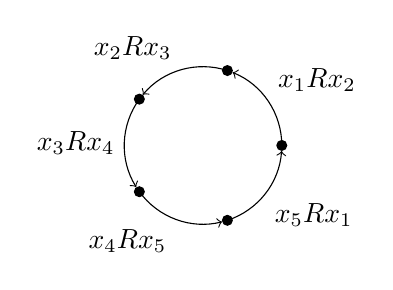
\begin{tikzpicture}
		\fill(1,0)circle(2pt)coordinate(A0);
		\fill({cos(72)},{sin(72)})circle(2pt)coordinate(A1);
		\fill({cos(144)},{sin(144)})circle(2pt)coordinate(A2);
		\fill({cos(216)},{sin(216)})circle(2pt)coordinate(A3);
		\fill({cos(288)},{sin(288)})circle(2pt)coordinate(A4);
		\begin{scope}[->]
			\draw(A0)arc[start angle=0,end angle=68,radius=1]node[midway,above right]{\(x_1 \rel{R} x_2\)};
			\draw(A1)arc[start angle=72,end angle=140,radius=1]node[midway,above left]{\(x_2 \rel{R} x_3\)};
			\draw(A2)arc[start angle=144,end angle=212,radius=1]node[midway,left]{\(x_3 \rel{R} x_4\)};
			\draw(A3)arc[start angle=216,end angle=284,radius=1]node[midway,below left]{\(x_4 \rel{R} x_5\)};
			\draw(A4)arc[start angle=288,end angle=356,radius=1]node[midway,below right]{\(x_5 \rel{R} x_1\)};
		\end{scope}
	\end{tikzpicture}
\end{center}
这是因为,如果我们有这样的环形成立,
那么根据传递性必有\(x_1 \rel{R} x_1\),
而这就与反自反性矛盾!

\begin{example}
设\(\rel{R}\)是\(A\)上的一个线性序,
证明:\(\rel{R}^{-1}\)也是\(A\)上的线性序.
\begin{proof}
由于\[
	\bigl( x \rel{R} y \land y \rel{R} z \implies x \rel{R} z \bigr)
	\iff
	\bigl( y \rel{R}^{-1} x \land z \rel{R}^{-1} y \implies z \rel{R}^{-1} x \bigr),
\]
可知\(\rel{R}^{-1}\)具有传递性.
又因为\(\rel{R}\)是\(A\)上的线性序,
所以对于\(\forall x,y \in A\),以下三个命题\[
	x \rel{R} y, \qquad
	x = y, \qquad
	y \rel{R} x
\]有且仅有一个成立;
换句话说,以下三个命题\[
	y \rel{R}^{-1} x, \qquad
	x = y, \qquad
	x \rel{R}^{-1} y
\]有且仅有一个成立;
可知\(\rel{R}^{-1}\)服从三一律.
综上所述,\(\rel{R}^{-1}\)也是\(A\)上的线性序.
\end{proof}
\end{example}



\chapter{数列极限}
\section{数列极限的概念}
\begin{definition}
%@see: 《高等数学(第六版 上册)》 P26 定义1
%@see: 《数学分析(上册)》(陈纪修) P34 定义2.2.1
设\(\{x_n\}\)为一数列.
如果存在常数\(a\),
对于任意给定的正数\(\epsilon\)(不论它多么小),
总存在正整数\(N\),
使得当\(n > N\)时,
不等式\(\abs{x_n - a} < \epsilon\)都成立,
那么就称“数列\(\{x_n\}\)是\DefineConcept{收敛的}(convergent)”
或“数列\(\{x_n\}\) \DefineConcept{收敛}(converge)”;
称常数\(a\)为“\(\{x_n\}\)的\DefineConcept{极限}(limit)”;
又称“数列\(\{x_n\}\) \DefineConcept{收敛于} \(a\)”;
记为\(\lim_{n\to\infty} x_n = a\)
或\(x_n\to a\ (n\to\infty)\).
否则,称“数列\(\{x_n\}\)没有极限”
或“数列\(\{x_n\}\)是\DefineConcept{发散的}(divergent)”
或“数列\(\{x_n\}\) \DefineConcept{发散}(diverge)”
或“极限\(\lim_{n\to\infty} x_n\)不存在”.
\end{definition}

上面定义中正数\(\epsilon\)可以任意给定是很重要的,
因为只有这样,不等式\(\abs{x_n - a} < \epsilon\)才能表达出\(x_n\)与\(a\)“无限接近”的意思.
此外还应注意到:
定义中的正整数\(N\)是与任意给定的正数\(\epsilon\)有关的,
它随着\(\epsilon\)的给定而选定.

利用形式逻辑的语言,我们可以将上述定义简化为:
\begin{align*}
	\text{数列\(\{x_n\}\)收敛于\(a\)}
	&\defiff
	\lim_{n\to\infty} x_n = a \\
	&\defiff
	(\forall \epsilon > 0)
	(\exists N\in\mathbb{N})
	(\forall n\in\mathbb{N})
	[
		n > N
		\implies
		\abs{x_n - a} < \epsilon
	]; \\
	\text{数列\(\{x_n\}\)收敛}
	&\defiff
	(\exists a\in\mathbb{R})
	\left[
		\lim_{n\to\infty} x_n = a
	\right].
\end{align*}
并且我们有\[
	\text{数列\(\{x_n\}\)发散}
	\iff
	(\forall a \in \mathbb{R})
	(\exists\epsilon>0)
	(\forall N\in\mathbb{N})
	(\exists n > N)
	[
		\abs{a_n - a} > \epsilon
	].
\]

\begin{proposition}
设\(a,b\)是实常数,对于数列\(\{x_n\}\),
有\[
	\lim_{n\to\infty} x_n = a
	\iff
	\lim_{n\to\infty} (x_n + b) = a + b.
\]
\begin{proof}
根据数列极限的定义有\begin{align*}
	&\lim_{n\to\infty} x_n = a \\
	&\iff
	(\forall \epsilon > 0)
	(\exists N\in\mathbb{N})
	(\forall n\in\mathbb{N})
	[
		n > N
		\implies
		\abs{x_n - a} < \epsilon
	] \\
	&\iff
	(\forall \epsilon > 0)
	(\exists N\in\mathbb{N})
	(\forall n\in\mathbb{N})
	[
		n > N
		\implies
		\abs{(x_n+b) - (a+b)} < \epsilon
	] \\
	&\iff
	\lim_{n\to\infty} (x_n+b) = a+b.
	\qedhere
\end{align*}
\end{proof}
\end{proposition}

\begin{example}
证明数列\[
2,\frac{1}{2},\frac{4}{3},\frac{3}{4},\dotsc,\frac{n+(-1)^{n-1}}{n},\dotsc
\]的极限是1.
\begin{proof}
由于\[
\abs{x_n - 1}
= \abs{\frac{n+(-1)^{n-1}}{n}-1}
= \abs{\frac{(-1)^{n-1}}{n}}
= \frac{1}{n},
\]所以为使\(\abs{x_n - 1} < \epsilon\),须取\(\frac{1}{n} < \epsilon\)或\(\frac{1}{\epsilon} < n\).
也就是说,对于\(\forall \epsilon > 0\),取\(N = \floor*{\frac{1}{\epsilon}}\),则当\(n > N\)时,就有\(\abs{x_n - a} < \epsilon\),即\(\lim_{n\to\infty}\frac{n+(-1)^{n-1}}{n}=1\).
\end{proof}
\end{example}

\begin{example}
已知\(x_n = \frac{(-1)^n}{(n+1)^2}\),证明数列\(\Set{x_n}\)的极限是\(0\).
\begin{proof}
因为\(\abs{x_n - a} = \abs{\frac{(-1)^n}{(n+1)^2}-0} = \frac{1}{(n+1)^2} < \frac{1}{n+1}\),所以对于\(\forall\epsilon>0\)(设\(\epsilon<1\)),只要\(\frac{1}{n+1}<\epsilon\)或\(n>\frac{1}{\epsilon}-1\),不等式\(\abs{x_n-a}<\epsilon\)必定成立.所以,取\(N=\floor*{\frac{1}{\epsilon}-1}\),则当\(n>N\)时就有\(\abs{x_n - a}<\epsilon\),即\(\lim_{n\to\infty}\frac{(-1)^n}{(n+1)^2}=0\).
\end{proof}
\end{example}

在利用数列极限的定义来论证某个数\(a\)是数列\(\{x_n\}\)的极限时,
重要的是对于任意给定的正数\(\epsilon\),要能够指出定义中所说的这种正整数\(N\)确实存在,
但没有必要去求最小的\(N\).
如果知道\(\abs{x_n-a}\)小于某个量(这个量是\(n\)的一个函数),
那么当这个量小于\(\epsilon\)时,\(\abs{x_n-a}<\epsilon\)当然也成立.
若令这个量小于\(\epsilon\)来定出\(N\)比较方便的话,就可采用这种方法.

\begin{example}
%@see: 《数学分析(上册)》(陈纪修) P36 例2.2.2
设\(\abs{q}<1\),
证明等比数列\[
	1,q,q^2,\dotsc,q^{n-1},\dotsc
\]的极限是\(0\).
\begin{proof}
对于\(\forall\epsilon>0\)(设\(\epsilon<1\)),
因为\(\abs{x_n-0}=\abs{q^{n-1}-0}=\abs{q}^{n-1}\),
要使\(\abs{x_n-0}<\epsilon\),
只要\(\abs{q}^{n-1}<\epsilon\).
取自然对数得\((n-1)\ln\abs{q}<\ln\epsilon\).
因为\(\abs{q}<1\),
\(\ln\abs{q}<0\),
故\(n>1+\frac{\ln\epsilon}{\ln\abs{q}}\).
取\(N=\floor*{1+\frac{\ln\epsilon}{\ln\abs{q}}}\),
则当\(n>N\)时,
就有\(\abs{q^{n-1}-0}<\epsilon\),
即
\begin{equation}
	\lim_{n\to\infty}q^{n-1}=0
	\quad(\abs{q}<1).
\end{equation}
由此可知,当\(\abs{q}<1\)时,
等比数列\(1,q,q^2,\dotsc,q^{n-1},\dotsc\)的极限是\(0\).
\end{proof}
\end{example}

\begin{example}\label{example:极限.常数的方根的极限1}
%@see: 《数学分析(上册)》(陈纪修) P36 例2.2.3
设\(a>1\),证明:\(\lim_{n\to\infty} \sqrt[n]{a} = 1\).
\begin{proof}
记\(y_n=\sqrt[n]{a}-1\).
因为\(a>1\),所以对于\(n\geq1\)总有\(\sqrt[n]{a}>1\),即\(y_n>0\).
应用二项式定理,有\[
	a = (1+y_n)^n
	= 1 + n y_n + \frac{n(n-1)}2 y_n^2 + \dotsb + y_n^n
	> 1 + n y_n,
\]
于是\(\abs{\sqrt[n]{a}-1} = \abs{y_n} < \frac{a-1}{n}\).
那么对于\(\forall\epsilon>0\),只要取\(N=\ceil*{\frac{a-1}{\epsilon}}\),
当\(n>N\)时就有\(\abs{\sqrt[n]{a}-1} < \frac{a-1}{n} < \epsilon\)成立.
同理可证当\(0<a<1\)时,也有\(\lim_{n\to\infty} \sqrt[n]{a} = 1\).
\end{proof}
\end{example}

\begin{example}
%@see: 《数学分析(上册)》(陈纪修) P37 例2.2.4
证明:\begin{equation}
	\lim_{n\to\infty} \sqrt[n]{n} = 1.
\end{equation}
\begin{proof}
要证\(\lim_{n\to\infty} \sqrt[n]{n} = 1\),
只需证对于\(\forall\epsilon>0\),
\(\exists N > 0\),
使得当\(n > N\)时,
有\[
	\abs{\sqrt[n]{n} - 1} < \epsilon.
	\eqno(1)
\]

因为\(n \geq 1\),
\(\sqrt[n]{n} \geq 1\),
所以(1)式等价于\[
	\abs{\sqrt[n]{n} - 1}
	= \sqrt[n]{n} - 1
	< \epsilon,
\]
也即\(\sqrt[n]{n} < 1 + \epsilon\),
取对数得\[
	\frac{1}{n} \ln n < \ln(1+\epsilon);
	\eqno(2)
\]
又因为\(\ln n < \sqrt{n}\),
所以只要有\[
	\frac{1}{n} \ln n
	< \frac{1}{n} \sqrt{n}
	= \frac{1}{\sqrt{n}}
	\leq \ln(1+\epsilon)
	\quad\text{或}\quad
	n \geq \left[ \frac1{\ln(1+\epsilon)} \right]^2
	\eqno(3)
\]
成立即有(2)式成立,
那么取\[
	N = \ceil*{\left[ \frac1{\ln(1+\epsilon)} \right]^2},
\]
就对\(\forall\epsilon>0\),
\(\exists N > 0\),
使得当\(n > N\)时,
有\(\abs{\sqrt[n]{n} - 1} < \epsilon\)成立.
\end{proof}
\end{example}

\begin{example}\label{example:极限.数列的算术平均的极限}
%@see: 《数学分析(上册)》(陈纪修) P37 例2.2.6
设\(\lim_{n\to\infty} a_n = a\).
证明:\(\lim_{n\to\infty} \frac{a_1+a_2+\dotsb+a_n}{n} = a\).
\begin{proof}
下面按\(a\)的不同取值,分两种情况讨论:
\begin{itemize}
	\item 当\(a=0\)时,
	有\[
		\lim_{n\to\infty} a_n = 0
		\iff
		(\forall\epsilon>0)
		(\exists N_1\in\mathbb{N})
		(\forall n\in\mathbb{N})
		\left[n>N_1 \implies \abs{a_n}<\frac\epsilon2\right].
	\]
	由于\(a_1 + a_2 + \dotsb + a_{N_1}\)是与\(n\)无关的常量,
	因此\[
		(\forall\epsilon>0)
		(\exists N_2\in\mathbb{N})
		(\forall n\in\mathbb{N})
		\left[
			n>N_2
			\implies
			\abs{\frac{a_1 + a_2 + \dotsb + a_{N_1}}{n}} < \frac\epsilon2
		\right].
	\]
	于是利用三角不等式(\cref{theorem:不等式.三角不等式1,theorem:不等式.三角不等式1.推论1})可得,
	对于\(\forall\epsilon>0\),
	当\(n>N=\max\{N_1,N_2\}\)时,
	有\begin{align*}
		\abs{\frac{a_1 + a_2 + \dotsb + a_n}{n}}
		&= \abs{
			\frac{a_1 + a_2 + \dotsb + a_{N_1}}{n}
			+ \frac{a_{N_1+1} + a_{N_1+2} + \dotsb + a_n}{n}
		} \\
		&\leq \abs{\frac{a_1 + a_2 + \dotsb + a_{N_1}}{n}}
		+ \abs{\frac{a_{N_1+1} + a_{N_1+2} + \dotsb + a_n}{n}} \\
		&< \frac\epsilon2 + \frac1n (n-N_1) \frac\epsilon2
		< \frac\epsilon2 + \frac\epsilon2
		= \epsilon.
	\end{align*}

	\item 当\(a\neq0\)时,
	显然\(\lim_{n\to\infty} (a_n - a) = 0\),
	于是\[
		\lim_{n\to\infty} \left(\frac{a_1+a_2+\dotsb+a_n}{n}-a\right)
		= \lim_{n\to\infty} \frac{(a_1-a)+(a_2-a)+\dotsb+(a_n-a)}{n}
		= 0,
	\]
	也就是说\(\lim_{n\to\infty} \frac{a_1+a_2+\dotsb+a_n}{n} = a\).
	\qedhere
\end{itemize}
\end{proof}
\end{example}

\begin{proposition}\label{theorem:极限.数列的绝对值的极限}
设数列\(\{x_n\}\)的极限\(\lim_{n\to\infty} x_n\)存在,
则\(\lim_{n\to\infty} \abs{x_n} = \abs{\lim_{n\to\infty} x_n}\).
\begin{proof}
假设\(\lim_{n\to\infty} x_n = a\),
那么\((\forall\epsilon>0)
(\exists N\in\mathbb{N})
(\forall n\in\mathbb{N})
[n>N \implies \abs{x_n - a} < \epsilon]\);
由\hyperref[theorem:不等式.三角不等式2]{三角不等式}有
\(\abs{\abs{x_n} - \abs{a}} \leq \abs{x_n - a}\),
于是有\(\abs{\abs{x_n} - \abs{a}} < \epsilon\),
也就是说\(\lim_{n\to\infty} \abs{x_n} = \abs{a}\).
\end{proof}
\end{proposition}

\begin{example}\label{example:极限.指标变化时数列极限不变}
%@see: 《数学分析(上册)》(陈纪修) P45 习题 4.
设\(k\in\mathbb{N}^+\).
证明:\(\lim_{n\to\infty} x_n = a \iff \lim_{n\to\infty} x_{n+k} = a\).
\begin{proof}
假设\(\lim_{n\to\infty} x_n = a\).
根据定义,对于\(\forall\epsilon>0\),
存在正整数\(N\),只要\(n>N\),就有\(\abs{x_n-a}<\epsilon\).
因为\(n+k>n\),所以\(\abs{x_{n+k}-a}<\epsilon\)必然成立,
从而有\(\lim_{n\to\infty} x_{n+k} = a\).

假设\(\lim_{n\to\infty} x_{n+k} = a\).
同样根据定义,对于\(\forall\epsilon>0\),
存在正整数\(N\),只要\(n>N\),
或者说只要\(m=n+k>N+k\),
就有\(\abs{x_m-a}<\epsilon\),
于是有\(\lim_{m\to\infty} x_m = a\).
\end{proof}
\end{example}

\begin{example}
%@see: 《数学分析(上册)》(陈纪修) P45 习题 5.
%@see: 《高等数学(第六版 上册)》 P31 习题1-2 6.
设\(\lim_{k\to\infty} x_{2k} = \lim_{k\to\infty} x_{2k+1} = a\),
证明:\(\lim_{n\to\infty} x_n = a\).
\begin{proof}
由于\begin{gather*}
	\lim_{k\to\infty} x_{2k} = a
	\iff
	(\forall\epsilon>0)
	(\exists N_1\in\mathbb{N})
	(\forall k\in\mathbb{N})
	[
		k>N_1
		\implies
		\abs{x_{2k}-a}<\epsilon
	], \\
	\lim_{k\to\infty} x_{2k+1} = a
	\iff
	(\forall\epsilon>0)
	(\exists N_2\in\mathbb{N})
	(\forall k\in\mathbb{N})
	[
		k>N_2
		\implies
		\abs{x_{2k+1}-a}<\epsilon
	],
\end{gather*}
所以,只要\(k>N=\max\{N_1,N_2\}\),
就有\(\abs{x_{2k}-a}<\epsilon\)和\(\abs{x_{2k+1}-a}<\epsilon\)同时成立;
这就是说,只要\(n>2N+1\),
就有\(\abs{x_n-a}<\epsilon\)成立;
因此\(\lim_{n\to\infty} x_n = a\).
\end{proof}
\end{example}

\section{数列极限的性质}
\subsection{唯一性}
\begin{theorem}[唯一性]\label{theorem:极限.收敛数列的唯一性}
%@see: 《高等数学(第六版 上册)》 P28 定理1
%@see: 《数学分析(上册)》(陈纪修) P39 定理2.2.1
如果数列\(\{x_n\}\)收敛,那么它的极限唯一.
\begin{proof}
用反证法.
假设当\(n\to\infty\)时,同时有\(x_n \to a\)及\(x_n \to b\),且\(a < b\).
取\(\epsilon = \frac{b-a}{2}\).
因为\(\lim_{n\to\infty}x_n = a\),所以有
\[
	(\exists N_1\in\mathbb{N})
	(\forall n\in\mathbb{N})
	\left[n > N_1 \implies \abs{x_n - a} < \frac{b-a}{2}\right]
	\eqno(1)
\]成立.

同理,因为\(\lim_{n\to\infty}x_n = b\),所以有
\[
	(\exists N_2 \in \mathbb{N})
	(\forall n\in\mathbb{N})
	\left[n > N_2 \implies \abs{x_n - b} < \frac{b-a}{2}\right]
	\eqno(2)
\]成立.

取\(N = \max\{N_1,N_2\}\),则当\(n > N\)时,上述两个不等式应同时成立.
但由(1)式有\(x_n<\frac{a+b}{2}\),由(2)式有\(x_n>\frac{a+b}{2}\),
矛盾,故收敛数列的极限必定唯一.
\end{proof}
\end{theorem}

\begin{example}\label{example:极限.振荡数列不存在极限}
证明数列\(x_n=(-1)^{n+1}\ (n=1,2,\dotsc)\)是发散的.
\begin{proof}
假设这级数收敛,则它具有唯一的极限\(\lim_{n\to\infty}x_n = a\).
按数列极限的定义,对于\(\epsilon=1/2\),\(\exists N \in \mathbb{N}^+\),当\(n > N\)时,\(\abs{x_n-a}<1/2\)或\(x_n\in\left(a-\frac{1}{2},a+\frac{1}{2}\right)\)成立.
但这是不可能的,因为\(n\to\infty\)时,\(x_n\)无休止地一再重复取得\(1\)和\(-1\)这两个数,而这两个数不可能同时属于长度为\(1\)的开区间\(\left(a-\frac{1}{2},a+\frac{1}{2}\right)\)内,因此这数列发散.
\end{proof}
\end{example}

\subsection{有界性}
\begin{theorem}[有界性]\label{theorem:极限.收敛数列的有界性}
%@see: 《高等数学(第六版 上册)》 P29 定理2
%@see: 《数学分析(上册)》(陈纪修) P39 定理2.2.2
如果数列\(\{x_n\}\)收敛,
那么数列\(\{x_n\}\)一定有界.
\begin{proof}
既然数列\(\{x_n\}\)收敛,
不妨设\(\lim_{n\to\infty}x_n = a\).
根据数列极限的定义,
对于\(\epsilon = 1\),
\(\exists N \in \mathbb{N}^+\),
当\(n > N\)时,
不等式\(\abs{x_n - a} < 1\)都成立.
于是,
当\(n > N\)时,
\[
	\abs{x_n} = \abs{(x_n - a) + a} \leq \abs{x_n - a} + \abs{a} < 1 + \abs{a}.
\]
取\(M = \max\{\abs{x_1},\abs{x_2},\dotsc,\abs{x_N},1+\abs{a}\}\),
那么数列\(\{x_n\}\)中的一切\(x_n\)都满足不等式\[
	\abs{x_n} \leq M.
\]
这就证明了数列\(\{x_n\}\)是有界的.
\end{proof}
\end{theorem}

根据\cref{theorem:极限.收敛数列的有界性} 立即有以下推论.
\begin{corollary}
如果数列\(\{x_n\}\)是无界的,那么数列\(\{x_n\}\)一定发散.
\end{corollary}
但是,如果数列\(\{x_n\}\)有界,却不能断定数列\(\{x_n\}\)一定收敛.
例如,在\cref{example:极限.振荡数列不存在极限} 中,
数列\[
	1,-1,1,\dotsc,(-1)^{n+1},\dotsc
\]有界,
但它是发散的.
于是我们可以说:
数列有界是数列收敛的必要不充分条件.

\subsection{保序性}
\begin{theorem}[保序性]\label{theorem:极限.收敛数列的保序性}
%@see: 《数学分析(上册)》(陈纪修) P39 定理2.2.3
设数列\(\{x_n\},\{y_n\}\)均收敛.
若\(\lim_{n\to\infty} x_n = a,
\lim_{n\to\infty} y_n = b\),
且\(a < b\),
则存在正整数\(N\),当\(n>N\)时,
有\(x_n < y_n\).
\begin{proof}
取\(\epsilon=\frac{b-a}2>0\),
则\[
	\lim_{n\to\infty} x_n = a
	\implies
	(\exists N_1\in\mathbb{N})(\forall n\in\mathbb{N})
	\left[
		\begin{array}{rl}
			n>N_1
			&\implies
			\abs{x_n - a} < \epsilon = \frac{b-a}2 \\
			&\implies
			x_n < a + \frac{b-a}2 = \frac{a+b}2
		\end{array}
	\right],
\]\[
	\lim_{n\to\infty} y_n = b
	\implies
	(\exists N_2\in\mathbb{N})(\forall n\in\mathbb{N})
	\left[
		\begin{array}{rl}
			n>N_2
			&\implies
			\abs{y_n - b} < \epsilon = \frac{b-a}2 \\
			&\implies
			y_n > b - \frac{b-a}2 = \frac{a+b}2
		\end{array}
	\right],
\]
于是,取\(N = \max\{N_1,N_2\}\),
则对\(\forall n\in\mathbb{N}\),
只要\(n>N\),
就有\(x_n < \frac{a+b}2 < y_n\).
\end{proof}
\end{theorem}

\begin{corollary}[保号性]\label{theorem:极限.收敛数列的保号性}
%@see: 《高等数学(第六版 上册)》 P29 定理3
%@see: 《数学分析(上册)》(陈纪修) P40 推论
设\(\lim_{n\to\infty}x_n = a\).
\begin{itemize}
	\item 若\(a > 0\),
	那么\((\exists N\in\mathbb{N})
	(\forall n\in\mathbb{N})
	[n>N \implies x_n > 0]\).

	\item 若\(a < 0\),
	那么\((\exists N\in\mathbb{N})
	(\forall n\in\mathbb{N})
	[n>N \implies x_n < 0]\).
\end{itemize}
\begin{proof}
当\(a > 0\)时,
由数列极限的定义,
对\(\epsilon = \frac{a}{2} > 0\),
\(\exists N \in \mathbb{N}^+\),
当\(n > N\)时,
有\(\abs{x_n - a} < \frac{a}{2}\),
从而\(x_n > a - \frac{a}{2} = \frac{a}{2} > 0\).

同样地,
当\(a < 0\)时,
对\(\epsilon = -\frac{a}{2} > 0\),
\(\exists N \in \mathbb{N}^+\),
当\(n > N\)时,
有\(\abs{x_n - a} < -\frac{a}{2}\),
从而\(x_n < a - \frac{a}{2} = \frac{a}{2} < 0\).
\end{proof}
\end{corollary}

需要注意到,\cref{theorem:极限.收敛数列的保序性} 的逆命题不成立,
也就是说,由\[
	\lim_{n\to\infty} x_n = a, \qquad
	\lim_{n\to\infty} y_n = b, \qquad
	(\exists N\in\mathbb{N})
	(\forall n\in\mathbb{N})
	[n>N \implies x_n < y_n]
\]这三个条件,
无法推出\(a<b\)的结论.
数列\(\{x_n = 1/n\}\)和\(\{y_n = 2/n\}\)就是例子.
因此,我们只能得到如下结论:
\begin{proposition}\label{theorem:数列极限.夹逼准则.引理}
%@see: 《数学分析(上册)》(陈纪修) P41
设\(\lim_{n\to\infty} x_n = a,
\lim_{n\to\infty} y_n = b\).
若\((\exists N\in\mathbb{N})
(\forall n\in\mathbb{N})
[n>N \implies x_n < y_n]\),
则\(a \leq b\).
\end{proposition}

\begin{corollary}
%@see: 《高等数学(第六版 上册)》 P30 推论
设\(\lim_{n\to\infty} x_n = a\).
\begin{itemize}
	\item 若\((\exists N\in\mathbb{N})
	(\forall n\in\mathbb{N})
	[n > N \implies x_n \geq 0]\),
	那么\(a \geq 0\).

	\item 若\((\exists N\in\mathbb{N})
	(\forall n\in\mathbb{N})
	[n > N \implies x_n \leq 0]\),
	那么\(a \leq 0\).
\end{itemize}
\end{corollary}

\begin{example}
%@see: 《高等数学(第六版 上册)》 P31 习题1-2 5.
设数列\(\{x_n\}\)有界,又\(\lim_{n\to\infty} y_n = 0\).
证明:\(\lim_{n\to\infty} x_n y_n = 0\).
\begin{proof}
因为\[
	\text{数列\(\{x_n\}\)有界}
	\iff
	(\exists M>0)
	(\forall n\in\mathbb{N})
	[\abs{x_n} \leq M],
\]
又因为\(\lim_{n\to\infty} y_n = 0\),
所以\[
	(\forall \epsilon>0)
	(\exists N\in\mathbb{N})
	(\forall n\in\mathbb{N})
	\left[
		\begin{array}{l}
			n>N
			\implies
			\abs{y_n - 0}
				= \abs{y_n}
				< \frac{\epsilon}{M} \\
			\implies
			\abs{x_n y_n - 0}
			= \abs{x_n y_n}
			= \abs{x_n} \abs{y_n}
			< M \cdot \frac{\epsilon}{M}
			= \epsilon
		\end{array}
	\right].
\]
因此\(\lim_{n\to\infty} x_n y_n = 0\).
\end{proof}
\end{example}

\section{夹逼准则}
\begin{theorem}\label{theorem:数列极限.夹逼准则}
%@see: 《数学分析(第二版 上册)》(陈纪修) P41 定理2.2.4
%@see: 《高等数学(第六版 上册)》 P50 准则I
如果数列\(\{x_n\}\)、\(\{y_n\}\)及\(\{z_n\}\)满足
\begin{itemize}
	\item \((\exists n_0\in\mathbb{N})
	(\forall n\in\mathbb{N})
	[y_n \leq x_n \leq z_n]\),
	\item \(\lim_{n\to\infty} y_n = \lim_{n\to\infty} z_n = a\),
\end{itemize}
那么\(\lim_{n\to\infty} x_n = a\).
\begin{proof}
因为\(\lim_{n\to\infty} y_n = a\),
\(\lim_{n\to\infty} z_n = a\),
根据数列极限的定义,
有\[
	(\forall\epsilon>0)
	(\exists N_1,N_2\in\mathbb{N})
	(\forall n\in\mathbb{N})
	\left[
		\begin{array}{l}
			n > N_1 \implies \abs{y_n - a} < \epsilon, \\
			n > N_2 \implies \abs{z_n - a} < \epsilon
		\end{array}
	\right].
\]

现在取\(N = \max\{n_0,N_1,N_2\}\),
那么,当\(n > N\)时,有\[
	\left\{ \begin{array}{l}
		\abs{y_n - a} < \epsilon, \\
		\abs{z_n - a} < \epsilon,
	\end{array} \right.
	\quad\text{或}\quad
	\left\{ \begin{array}{l}
		a - \epsilon < y_n, \\
		z_n < a + \epsilon
	\end{array} \right.
\]同时成立.

又因当\(n > N\)时,有\[
	a - \epsilon < y_n \leq x_n \leq z_n < a + \epsilon,
\]即\[
	\abs{x_n - a} < \epsilon
\]成立.

综上所述,\[
	(\forall\epsilon>0)
	(\exists N\in\mathbb{N})
	(\forall n\in\mathbb{N})
	[
		n > N
		\implies
		\abs{x_n - a} < \epsilon
	];
\]
这就证明了\(\lim_{n\to\infty} x_n = a\).
\end{proof}
\end{theorem}

\begin{example}
%@see: 《数学分析(第二版 上册)》(陈纪修) P41 例2.2.7
求数列\(\{\sqrt{n+1}-\sqrt{n}\}\)的极限.
\begin{solution}
首先我们有\[
	\sqrt{n+1}-\sqrt{n}
	= \frac{(\sqrt{n+1}-\sqrt{n})(\sqrt{n+1}+\sqrt{n})}{\sqrt{n+1}+\sqrt{n}}
	= \frac1{\sqrt{n+1}+\sqrt{n}}.
\]
由于\[
	0 < \frac1{\sqrt{n+1}+\sqrt{n}} < \frac1{\sqrt{n}}, \qquad
	\lim_{n\to\infty} 0 = \lim_{n\to\infty} \frac1{\sqrt{n}} = 0,
\]
所以利用\hyperref[theorem:数列极限.夹逼准则]{夹逼准则}可得
\(\lim_{n\to\infty} (\sqrt{n+1}-\sqrt{n}) = 0\).
\end{solution}
\end{example}

\begin{example}
%@see: 《数学分析(第二版 上册)》(陈纪修) P42 例2.2.8
证明:\[
	\lim_{n\to\infty} (a_1^n + a_2^n + \dotsb + a_p^n)^{\frac1n}
	= \max_{1\leq i\leq p} \{a_i\},
\]
其中\(a_i\geq0\ (i=1,2,\dotsc,p)\).
\begin{proof}
不失一般性,设\(a_1 = \max_{1\leq i\leq p} \{a_i\}\),
于是\[
	a_1 \leq (a_1^n + a_2^n + \dotsb + a_p^n)^{\frac1n} \leq a_1 \sqrt[n]{p}.
\]
因为\(\lim_{n\to\infty} \sqrt[n]{p} = 1\),
所以\(\lim_{n\to\infty} a_1 \sqrt[n]{p} = a_1\).
利用\hyperref[theorem:数列极限.夹逼准则]{夹逼准则}可得\[
	\lim_{n\to\infty} (a_1^n + a_2^n + \dotsb + a_p^n)^{\frac1n} = a_1.
	\qedhere
\]
\end{proof}
\end{example}

\begin{example}
证明:\begin{equation}\label{equation:数列极限.重要极限3}
	\lim_{n\to\infty} \sqrt[n]{k n} = 1
	\quad(k>0).
\end{equation}
\begin{proof}
当\(n \geq 3\)时,
将\(\sqrt[n]{k n}\)看作一个\(k\)、两个\(\sqrt{n}\)与\(n-3\)个\(1\)的几何平均值,
则有\[
	1 \leq \sqrt[n]{k n} = (k \cdot \sqrt{n}^2 \cdot 1^{n-3})^{1/n}
	< \frac{k + 2\sqrt{n} + n-3}{n}
	= 1 + \frac{2}{\sqrt{n}} + \frac{k-3}{n}.
\]
因为\[
	\lim_{n\to\infty} 1
	= \lim_{n\to\infty} \left(1 + \frac{2}{\sqrt{n}} + \frac{k-3}{n}\right) = 1,
\]
由夹逼定理可得\(\lim_{n\to\infty} \sqrt[n]{k n} = 1\).
\end{proof}
\end{example}

\begin{example}
%@see: 《数学分析(第二版 上册)》(陈纪修) P45 习题 8.(4)
求:\(\lim_{n\to\infty} \frac{1 \cdot 3 \cdot 5 \dotsm (2n-1)}{2 \cdot 4 \cdot 6 \dotsm (2n)}\).
\begin{solution}
因为\((2n)^2 = 4n^2 > 4n^2-1 = (2n-1)(2n+1)\),\(2n > \sqrt{(2n-1)(2n+1)}\),
所以\[
	2 > \sqrt{1 \cdot 3},
	4 > \sqrt{3 \cdot 5},
	6 > \sqrt{5 \cdot 7},
	\dotsc,
\]
故\[
	0 < \frac{1 \cdot 3 \cdot 5 \dotsm (2n-1)}{2 \cdot 4 \cdot 6 \dotsm (2n)}
	< \frac{1 \cdot 3 \cdot 5 \dotsm (2n-1)}{\sqrt{1 \cdot 3} \sqrt{3 \cdot 5} \sqrt{5 \cdot 7} \dotsm \sqrt{(2n-1)(2n+1)}}
	= \frac{1}{\sqrt{2n+1}}.
\]
又因为\(\lim_{n\to\infty} \frac{1}{\sqrt{2n+1}} = 0\),
所以\begin{equation}\label{equation:数列极限.重要极限4}
	\lim_{n\to\infty} \frac{1 \cdot 3 \cdot 5 \dotsm (2n-1)}{2 \cdot 4 \cdot 6 \dotsm (2n)} = 0.
\end{equation}
\end{solution}
\end{example}

\begin{example}
求:\(\lim_{n\to\infty} \frac{2 \cdot 4 \cdot 6 \dotsm (2n)}{1 \cdot 3 \cdot 5 \dotsm (2n+1)}\).
\begin{solution}
因为\[
	2 \cdot 4 < 3^2,
	4 \cdot 6 < 5^2,
	\dotsc,
	(2n-2)(2n) < (2n-1)^2,
	(2n)(2n+2) < (2n+1)^2,
\]
所以\begin{gather*}
	2 \cdot [4 \cdot 6 \dotsm \cdot (2n)]^2 \cdot (2n+2)
	< [3 \cdot 5 \dotsm (2n+1)]^2, \\
	[2 \cdot 4 \cdot 6 \dotsm (2n)]^2 \cdot (2n+2)
	< 2 \cdot [3 \cdot 5 \dotsm (2n+1)]^2, \\
	2 \cdot 4 \cdot 6 \dotsm (2n) \cdot \sqrt{2n+2}
	< \sqrt2 \cdot [3 \cdot 5 \dotsm (2n+1)], \\
	\frac{2 \cdot 4 \cdot 6 \dotsm (2n)}{1 \cdot 3 \cdot 5 \dotsm (2n+1)}
	< \frac{\sqrt2}{\sqrt{2n+2}}
	= \frac1{\sqrt{n+1}}.
\end{gather*}
又因为\(\lim_{n\to\infty} \frac1{\sqrt{n+1}} = 0\),
所以\begin{equation}\label{equation:数列极限.重要极限5}
	\lim_{n\to\infty} \frac{2 \cdot 4 \cdot 6 \dotsm (2n)}{1 \cdot 3 \cdot 5 \dotsm (2n+1)} = 0.
\end{equation}
\end{solution}
\end{example}

\begin{proposition}
设数列\(\{x_n\}\)满足\[
	\lim_{n\to\infty} \frac{x_{n+1}}{x_n} = \rho \in (-1,1),
\]
那么\(\lim_{n\to\infty} x_n = 0\).
\begin{proof}
因为\(\lim_{n\to\infty} \frac{x_{n+1}}{x_n} = \rho\),
所以根据数列极限的定义,
\(\forall\epsilon>0\),
\(\exists N\in\mathbb{N}\),
\(\forall n\in\mathbb{N}\),
只要\(n > N\),
就有\(\rho-\epsilon < \frac{x_{n+1}}{x_n} < \rho+\epsilon\).
取\(r=\max\{\abs{\rho-\epsilon},\abs{\rho+\epsilon}\}\),
那么有\(\abs{\frac{x_{n+1}}{x_n}} < r\),
即\(\abs{x_{n+1}} < r \abs{x_n}\),
于是\(0 \leq \abs{x_{n+k}} < r^k \abs{x_n}\ (k=1,2,\dotsc)\);
又因为当\(\epsilon\)足够小时,必有\(0<r<1\),
所以\[
	\lim_{k\to\infty} r^k \abs{x_n} = 0;
\]
那么根据\hyperref[theorem:数列极限.夹逼准则]{夹逼准则},
\(\lim_{k\to\infty} \abs{x_{n+k}} = 0\);
由\cref{theorem:极限.数列的绝对值的极限} 可知\(\lim_{k\to\infty} x_{n+k} = 0\);
再由\cref{example:极限.指标变化时数列极限不变} 可知\(\lim_{n\to\infty} x_n = 0\).
\end{proof}
\end{proposition}

\section{数列极限的四则运算}
\begin{theorem}\label{theorem:极限.数列极限的四则运算法则}
%@see: 《高等数学(第六版 上册)》 P45 定理4
%@see: 《数学分析(第二版 上册)》(陈纪修) P42 定理2.2.5
设数列\(\{x_n\}\)和\(\{y_n\}\)
满足\(\lim_{n\to\infty} x_n = A\)
和\(\lim_{n\to\infty} y_n = B\),
那么\begin{enumerate}
	\item \(\lim_{n\to\infty} (x_n \pm y_n) = A \pm B\);
	\item \(\lim_{n\to\infty} (x_n \cdot y_n) = A \cdot B\);
	\item 当\(y_n \neq 0\ (n=1,2,\dotsc,)\)且\(B \neq 0\)时,
	\(\lim_{n\to\infty}{\frac{x_n}{y_n}}=\frac{A}{B}\).
\end{enumerate}
\end{theorem}

\begin{corollary}
%@see: 《数学分析(第二版 上册)》(陈纪修) P42 定理2.2.5
设\(\lim_{n\to\infty} x_n = A,
\lim_{n\to\infty} y_n = B\),
\(a,b\)是常数,
则\(\lim_{n\to\infty} (a x_n + b y_n) = a A + b B\).
\end{corollary}

\begin{example}\label{example:极限.常数的方根的极限2}
%@see: 《数学分析(第二版 上册)》(陈纪修) P43 例2.2.10
设\(a>0\),证明:\(\lim_{n\to\infty} \sqrt[n]{a} = 1\).
\begin{proof}
在\cref{example:极限.常数的方根的极限1} 中我们已经证明
当\(a>1\)时\(\lim_{n\to\infty} \sqrt[n]{a} = 1\).
当\(a=1\)时,\(\sqrt[n]{a}\)恒等于\(1\),从而也有\(\lim_{n\to\infty} \sqrt[n]{a} = 1\).
现在考虑\(0<a<1\),这时\(\frac1a>1\),从而\(\lim_{n\to\infty} \sqrt[n]{\frac1a} = 1\),
那么利用\hyperref[theorem:极限.数列极限的四则运算法则]{极限的四则运算法则}可得
\(\lim_{n\to\infty} \sqrt[n]{a}
= \lim_{n\to\infty} \frac1{\sqrt[n]{1/a}} = 1\).
\end{proof}
\end{example}

\begin{example}
%@see: 《数学分析(第二版 上册)》(陈纪修) P43 例2.2.11
求极限\(\lim_{n\to\infty} n(\sqrt{n^2+1}-\sqrt{n^2-1})\).
\begin{solution}
直接计算得\begin{align*}
	&\hspace{-20pt}
	\lim_{n\to\infty} n(\sqrt{n^2+1}-\sqrt{n^2-1})
	= \lim_{n\to\infty} \frac{2n}{\sqrt{n^2+1}+\sqrt{n^2-1}} \\ % 分子有理化
	&= \lim_{n\to\infty} \frac2{\sqrt{1+(1/n)^2}+\sqrt{1-(1/n)^2}} % 分子分母同时除以\(n\)
	= 1.
\end{align*}
\end{solution}
\end{example}

\begin{corollary}
%@see: 《数学分析(第二版 上册)》(陈纪修) P43
设\(\lim_{n\to\infty} x_{in} = A_i\ (i=1,2,\dotsc,m)\),
则\[
	\lim_{n\to\infty} \sum_{i=1}^m x_{in} = \sum_{i=1}^m A_i,
\]\[
	\lim_{n\to\infty} \prod_{i=1}^m x_{in} = \prod_{i=1}^m A_i.
\]
\end{corollary}

\begin{remark}
%@see: 《数学分析(第二版 上册)》(陈纪修) P43
数列极限的四则运算法则只能推广到有限个数列相加或相乘的情况,
不能随意推广到无限个数列上去.
例如,若将\cref{theorem:极限.数列极限的四则运算法则} 随意推广,
可能会得出极限\[
	\lim_{n\to\infty} \left(
		\frac1{\sqrt{n^2+1}}
		+ \frac1{\sqrt{n^2+2}}
		+ \dotsb + \frac1{\sqrt{n^2+n}}
	\right)
\]为\(0\)的错误结论;
但是,由于\[
	\frac{n}{\sqrt{n^2+n}}
	< \frac1{\sqrt{n^2+1}}
	+ \frac1{\sqrt{n^2+2}}
	+ \dotsb + \frac1{\sqrt{n^2+n}}
	< \frac{n}{\sqrt{n^2+1}},
\]
利用\hyperref[theorem:数列极限.夹逼准则]{夹逼准则}可知该极限其实为\(1\).
\end{remark}

\begin{example}\label{example:极限.收敛数列前n项积的n次方根}
%@see: 《数学分析(第二版 上册)》(陈纪修) P44 例2.2.12
设\(a_n>0\),\(\lim_{n\to\infty} a_n = a\),证明:
\(\lim_{n\to\infty} \sqrt[n]{a_1 a_2 \dotsm a_n} = a\).
\begin{proof}
应用\hyperref[theorem:不等式.均值不等式]{均值不等式}可得\[
	\frac{a_1+a_2+\dotsb+a_n}n
	\geq \sqrt[n]{a_1 a_2 \dotsm a_n}
	\geq n\left(\frac1{a_1}+\frac1{a_2}+\dotsb+\frac1{a_n}\right)^{-1}
	> 0.
\]
由\cref{example:极限.数列的算术平均的极限} 我们已经知道
\(\lim_{n\to\infty} \frac{a_1+a_2+\dotsb+a_n}{n} = a\).
要想利用\hyperref[theorem:数列极限.夹逼准则]{夹逼准则}证明上述问题,
就必须证明上面不等式中\(\sqrt[n]{a_1 a_2 \dotsm a_n}\)右边的数列极限也等于\(a\).

下面按\(a\)的不同取值,分两种情况讨论:
\begin{itemize}
	\item 当\(a=0\)时,
	有\(\sqrt[n]{a_1 a_2 \dotsm a_n} > 0 = a\).

	\item 当\(a>0\)时,
	由\hyperref[theorem:极限.数列极限的四则运算法则]{数列极限的四则运算法则}可知
	\(\lim_{n\to\infty} \frac1{a_n} = \frac1a\),
	故\[
		\lim_{n\to\infty} \frac1n \left(\frac1{a_1}+\frac1{a_2}+\dotsb+\frac1{a_n}\right) = \frac1a,
	\]
	从而
	\(\lim_{n\to\infty} n\left(\frac1{a_1}+\frac1{a_2}+\dotsb+\frac1{a_n}\right)^{-1} = a\).
\end{itemize}
在上述两种情况下,\(\sqrt[n]{a_1 a_2 \dotsm a_n}\)右边的数列极限都等于\(a\),
所以\(\lim_{n\to\infty} \sqrt[n]{a_1 a_2 \dotsm a_n} = a\).
\end{proof}
\end{example}

\begin{example}
%@see: 《数学分析(第二版 上册)》(陈纪修) P45 习题 8.(1)
求极限\(\lim_{n\to\infty} \sqrt[n]{1+\frac12+\dotsb+\frac1n}\).
\begin{solution}
首先我们有\(1 \leq 1+\frac12+\dotsb+\frac1n \leq n\),
因为\(\lim_{n\to\infty} \sqrt[n]{1} = \lim_{n\to\infty} \sqrt[n]{n} = 1\),
所以\[
	\lim_{n\to\infty} \sqrt[n]{1+\frac12+\dotsb+\frac1n} = 1.
\]
\end{solution}
\end{example}

\begin{example}
%@see: 《数学分析(第二版 上册)》(陈纪修) P45 习题 8.(2)
求极限\(\lim_{n\to\infty} \left(\frac1{n+\sqrt1}+\frac1{n+\sqrt2}+\dotsb+\frac1{n+\sqrt{n}}\right)\).
\begin{solution}
首先有\(\frac{n}{n+\sqrt{n}}
\leq \frac1{n+\sqrt1}+\frac1{n+\sqrt2}+\dotsb+\frac1{n+\sqrt{n}}
\leq \frac{n}{n+1}\).
因为\[
	\lim_{n\to\infty} \frac{n}{n+\sqrt{n}}
	= \lim_{n\to\infty} \frac{n}{n+1} = 1,
\]
所以\(\lim_{n\to\infty} \left(\frac1{n+\sqrt1}+\frac1{n+\sqrt2}+\dotsb+\frac1{n+\sqrt{n}}\right) = 1\).
\end{solution}
\end{example}

\begin{example}
%@see: 《数学分析(第二版 上册)》(陈纪修) P45 习题 9.(7)
求极限\(\lim_{n\to\infty} \sqrt[n]{\frac1{n!}}\).
\begin{solution}\let\qed\relax
\begin{proof}[解法一]
因为\(\lim_{n\to\infty} \frac1n = 0\),
所以由\cref{example:极限.收敛数列前n项积的n次方根} 可知
\(\lim_{n\to\infty} \sqrt[n]{\frac1{n!}}
= \lim_{n\to\infty} \sqrt[n]{\frac11 \cdot \frac12 \dotsm \frac1n}
= 0\).
\end{proof}
\begin{proof}[解法二]
注意到\[
	\left(\frac1{n!}\right)^2
	= \prod_{k=1}^n \frac1{(n-k+1)k},%首尾相乘
\]
而\(\frac1{(n-k+1)k} \leq \frac1n\),
\(\prod_{k=1}^n \frac1{(n-k+1)k} \leq \frac1{n^n}\),
\(\frac1{n!} \leq \sqrt{\frac1{n^n}}\),
\(0 < \sqrt[n]{\frac1{n!}} \leq \frac1{\sqrt{n}}\),
加之\(\lim_{n\to\infty} \frac1{\sqrt{n}} = 0\),
因此根据\hyperref[theorem:数列极限.夹逼准则]{夹逼准则}可得
\(\lim_{n\to\infty} \sqrt[n]{\frac1{n!}} = 0\).
\end{proof}
\end{solution}
\end{example}

\begin{example}
%@see: 《数学分析(第二版 上册)》(陈纪修) P45 习题 9.(8)
求极限\(\lim_{n\to\infty} \left(1-\frac1{2^2}\right) \left(1-\frac1{3^2}\right) \dotsm \left(1-\frac1{n^2}\right)\).
\begin{solution}
直接计算得\begin{align*}
	&\hspace{-20pt}
	\lim_{n\to\infty} \left(1-\frac1{2^2}\right) \left(1-\frac1{3^2}\right) \dotsm \left(1-\frac1{n^2}\right) \\
	&= \lim_{n\to\infty} \frac{1\cdot3}{2^2} \cdot \frac{2\cdot4}{3^2} \cdot \frac{3\cdot5}{4^2} \dotsm \frac{(n-2)n}{(n-1)^2} \cdot \frac{(n-1)(n+1)}{n^2} \\
	&= \lim_{n\to\infty} \frac{2n(n+1)}{2^2 n^2}
	= \lim_{n\to\infty} \frac{n+1}{2n}
	= \frac12.
\end{align*}
\end{solution}
\end{example}

\begin{example}
%@see: 《数学分析(第二版 上册)》(陈纪修) P45 习题 9.(9)
求极限\(\lim_{n\to\infty} \sqrt[n]{n \ln n}\).
\begin{solution}
因为\(n < n \ln n < n^2\ (n\geq3)\),
\(\lim_{n\to\infty} \sqrt[n]{n}
= \lim_{n\to\infty} \sqrt[n]{n^2} = 1\),
所以\(\lim_{n\to\infty} \sqrt[n]{n \ln n} = 1\).
\end{solution}
\end{example}


\chapter{极限}
\section{数列极限}
极限的概念是由于求某些实际问题的精确解答而产生的.
例如,我国数学家刘徽利用圆内接正多边形来推算圆的面积的方法 --- 割圆术,
就是极限思想在几何学上的应用.

\subsection{子列极限与上下极限}
上、下极限是数列极限的必要组成部分,
它们各有三种等价的描述方式,
或者说三种等价的定义.
给定一种定义后,
其余两种定义的内容可以命题或定理的形式得到证明.

\begin{definition}
在数列\(\{x_n\}\)中任意抽取无限多项并保持这些项在原数列\(\{x_n\}\)中的先后次序,
这样得到的一个数列\[
	x_{p_1},x_{p_2},\dotsc,x_{p_n},\dotsc
	\quad(1 \leq p_1 < p_2 < \dotsb)
\]
称为原数列\(\{x_n\}\)的\DefineConcept{子数列}(或\DefineConcept{子列}).
\end{definition}

\begin{definition}
若子列\(\{x_{p_n}\}\)满足\[
	\lim_{n\to\infty} x_{p_n} = \xi,
\]
则称数\(\xi\)为“数列\(\{x_n\}\)的\DefineConcept{子列极限}(或极限点、聚点)”.

数列\(\{x_n\}\)的最小子列极限称为“数列\(x_n\)的\DefineConcept{下极限}”,
记作\[
	\varliminf_{n\to\infty} x_n
	\quad\text{或}\quad
	\liminf_{n\to\infty} x_n.
\]

数列\(\{x_n\}\)的最大子列极限称为“数列\(x_n\)的\DefineConcept{上极限}”,
记作\[
	\varlimsup_{n\to\infty} x_n
	\quad\text{或}\quad
	\limsup_{n\to\infty} x_n.
\]
\end{definition}
上面对上下极限的定义可以利用“\(\epsilon-N\)语言”更加简洁精确地重新定义为\begin{align*}
	\varliminf_{n\to\infty} x_n = \alpha
	&\defiff
	(\forall\epsilon>0)
	(\exists N\in\mathbb{N})
	(\forall n\in\mathbb{N})
	[
		n>N
		\implies
		\alpha-\epsilon < x_n
	]; \\
	\varlimsup_{n\to\infty} x_n = \beta
	&\defiff
	(\forall\epsilon>0)
	(\exists N\in\mathbb{N})
	(\forall n\in\mathbb{N})
	[
		n>N
		\implies
		x_n < \beta+\epsilon
	].
\end{align*}

\begin{theorem}[波尔查诺--魏尔斯特拉斯原理]\label{theorem:极限.波尔查诺--魏尔斯特拉斯原理}
任何有界数列至少有一个有限的子列极限.
\end{theorem}

\begin{theorem}\label{theorem:极限.上下极限的等价定义1}
数列\(\{x_n\}\)的上下极限满足:\[
	\varliminf_{n\to\infty} x_n
	= \lim_{n\to\infty} \inf\{x_n,x_{n+1},\dotsc\},
\]\[
	\varlimsup_{n\to\infty} x_n
	= \lim_{n\to\infty} \sup\{x_n,x_{n+1},\dotsc\}.
\]
\end{theorem}
\cref{theorem:极限.上下极限的等价定义1}
也是数列的上下极限的一种等价定义.

\begin{theorem}[收敛数列与其子列的关系]\label{theorem:子列极限.数列收敛的充分必要条件}
%@see: 《高等数学(第六版 上册)》 P30 定理4
如果数列\(\{x_n\}\)收敛于\(a\),
那么它的任一子列也收敛于\(a\).
\begin{proof}
设数列\(\{x_{n_k}\}\)是数列\(\{x_n\}\)的任一子数列.
由于\(\lim_{n\to\infty}x_n = a\),
故\(\forall \epsilon > 0\),
\(\exists N \in \mathbb{N}^+\),
当\(n > N\)时,
\(\abs{x_n - a} < \epsilon\)成立.
取\(K = N\),
则当\(k > K\)时,
由\(n_k > n_K \geq N\)
得\(\abs{x_{n_k} - a} < \epsilon\),
也就是说\(\lim_{k\to\infty}x_{n_k} = a\).
\end{proof}
\end{theorem}
由此可知,如果数列\(\{x_n\}\)的两个子列收敛于不同的极限,那么数列\(\{x_n\}\)是发散的.
例如数列\(\{x_n=(-1)^{n+1}\}\)的子数列\(\{x_{2k-1}\}\)收敛于\(1\),
而其子数列\(\{x_{2k}\}\)收敛于\(-1\),因此数列\(\{x_n\}\)是发散的.
同时这个例子也说明,一个发散的数列也可能有收敛的子数列.

\begin{corollary}
对于数列\(\{x_n\}\),
总有\[
	\lim_{n\to\infty} x_n = a
	\iff
	\varliminf_{n\to\infty} x_n
	= \varlimsup_{n\to\infty} x_n
	= a.
\]
\end{corollary}

\begin{example}
若\(\lim_{n\to\infty} u_n = a\),
证明\(\lim_{n\to\infty} \abs{u_n} = \abs{a}\).
并举例说明:
如果数列\(\{\abs{x_n}\}\)有极限,
但数列\(\{x_n\}\)未必有极限.
\begin{proof}
因为\(\lim_{n\to\infty} u_n = a\),
所以对\(\forall\epsilon>0\),
\(\exists N \in \mathbb{N}^+\),
使得当\(n>N\)时,
有\(\abs{u_n-a}<\epsilon\)成立.
根据三角不等式有\(\abs{\abs{u_n}-\abs{a}} \leq \abs{u_n-a}\),
显然当\(n>N\)时,
也有\(\abs{\abs{u_n}-\abs{a}}<\epsilon\)成立,
即\(\lim_{n\to\infty} \abs{u_n} = \abs{a}\).

根据前面的例子,
数列\(x_n = (-1)^{n+1}\)发散,
但\(\abs{x_n} = \abs{(-1)^{n+1}} = 1\)收敛,
说明如果数列\(\{\abs{x_n}\}\)有极限,
但数列\(\{x_n\}\)未必有极限.
\end{proof}
\end{example}

\section{函数极限}
\subsection{函数极限的定义}





\subsection{子列极限与上下极限}
\begin{definition}\label{definition:极限.函数的子列极限和上下极限}
设函数\(f(x)\)在区间\(I\)上有定义.
如果数列\(\{x_n\}\)满足\[
	x_i \in I \quad (i=1,2,\dotsc,n),
\]且数列极限\(\lim_{n\to\infty}{x_n} = a\),
则称极限\(\lim_{n\to\infty}{f(x_n)}\)为
“函数\(f(x)\)在点\(a\)的\DefineConcept{子列极限}”.

这些子列极限中的最小值称作“函数\(f(x)\)在点\(a\)的\DefineConcept{下极限}”,
记作\[
	\varliminf_{x \to a} f(x)
	\quad\text{或}\quad
	\liminf_{x \to a} f(x).
\]

这些子列极限中的最大值称作“函数\(f(x)\)在点\(a\)的\DefineConcept{上极限}”,
记作\[
	\varlimsup_{x \to a} f(x)
	\quad\text{或}\quad
	\limsup_{x \to a} f(x).
\]
\end{definition}

\begin{property}
函数\(f(x)\)的上、下极限满足:\begin{gather}
\varlimsup_{x \to a} f(x) = \lim_{\delta\to0^+} \sup_{0<\abs{x-a}<\delta} f(x), \\
\varliminf_{x \to a} f(x) = \lim_{\delta\to0^+} \inf_{0<\abs{x-a}<\delta} f(x).
\end{gather}
\end{property}

\begin{theorem}
任意函数\(f(x)\)的上下极限总满足\[
\varliminf_{x \to a} f(x) \leq \varlimsup_{x \to a} f(x).
\]
\end{theorem}

\begin{theorem}
函数\(f(x)\)当\(x \to x_0\)时极限存在的充分必要条件是:其上极限和下极限相等,即\[
\varlimsup_{x \to a} f(x) = \varliminf_{x \to a} f(x) = A
\iff
\lim_{x \to a} f(x) = A.
\]
\end{theorem}

\section{函数极限与数列极限的关系,海涅定理}
\subsection{海涅定理}
\begin{theorem}[海涅定理]\label{theorem:极限.海涅定理}
%@see: 《数学分析(上册)》(陈纪修) P78 定理3.1.5
%@see: 《数学分析教程(第3版 上册)》(史济怀) P70 定理2.4.1
%@see: 《数学分析(第7版 第一卷)》(卓里奇) P92 命题1
设函数\(f\colon D\to\mathbb{R}\).
\(\lim_{x \to x_0} f(x) = A\)的充分必要条件是:
任何一个值域为\(D-\{x_0\}\)且收敛于\(x_0\)的数列\(\{x_n\}\)
总满足\(\lim_{n\to\infty} f(x_n) = A\).
\begin{proof}
必要性.
由\(\lim_{x \to x_0} f(x) = A\)可知\[
	(\forall\epsilon>0)
	(\exists\delta>0)
	(\forall x\in D)
	[
		0<\abs{x-x_0}<\delta
		\implies
		\abs{f(x)-A}<\epsilon
	].
\]
因为\(\lim_{n\to\infty} x_n = x_0\),
且\(x_n \neq x_0\ (n=1,2,\dotsc)\),
所以\[
	(\forall\delta>0)
	(\exists N\in\mathbb{N})
	(\forall n\in\mathbb{N})
	[
		n>N
		\implies
		0<\abs{x_n-x_0}<\delta
		\implies
		\abs{f(x_n)-A}<\epsilon
	],
\]
即\(\lim_{n\to\infty} f(x_n) = A\).

充分性.
用反证法.
我们知道,命题“函数\(f\)在点\(x_0\)的极限是\(A\)”可以表述为\[
	(\forall\epsilon>0)
	(\exists\delta>0)
	(\forall x\in D)
	[
		0<\abs{x-x_0}<\delta
		\implies
		\abs{f(x)-A}<\epsilon
	],
\]
那么它的否命题“函数\(f\)在点\(x_0\)的极限不是\(A\)”可以表述为\[
	(\exists\epsilon_0>0)
	(\forall\delta>0)
	(\exists x\in D)
	[
		0<\abs{x-x_0}<\delta
		\implies
		\abs{f(x)-A}\geq\epsilon_0
	].
\]
于是\[
	(\forall n\in\mathbb{N}^+)
	(\exists x_n\in D)
	\left[
		0<\abs{x_n-x_0}<\frac1n
		\implies
		\abs{f(x_n)-A}\geq\epsilon_0
	\right],
\]
如此,我们就找到了一个数列\(\{x_n\}\)
满足\(x_n\neq x_0\ (n=1,2,\dotsc)\)且\(\lim_{n\to\infty} x_n = x_0\),
但是\(\{f(x_n)\}\)不可能满足\(\lim_{n\to\infty} f(x_n) = A\).
由此推翻假设,得到\(\lim_{x\to x_0} f(x) = A\).
\end{proof}
\end{theorem}
海涅定理也称作\DefineConcept{归结原则}.

这里要注意定理的条件\(x_n \neq x_0\),
因为只要没有这个条件就不能保证海涅定理的结果成立,下面我们举例说明.
设\[
	f(x) = \left\{ \begin{array}{cl}
		2, & x\neq0, \\
		1, & x=0.
	\end{array} \right.
\]
又设点\(x_0\)与数列\(\{x_n\}\)满足\(x_0=x_n=0\ (n=1,2,\dotsc)\).
那么有\[
	\lim_{n\to\infty} x_n = 0,
	\quad\text{和}\quad
	\lim_{x\to0} f(x) = 2,
\]
但是\[
	\lim_{n\to\infty} f(x_n) = \lim_{n\to\infty} f(0) = 1.
\]这就说明不总有\[
	\lim_{n\to\infty} f(x_n)
	= \lim_{x \to x_0} f(x)
\]成立.

\begin{example}
函数\(f\)在\((-\infty,+\infty)\)内单调有界,
数列\(\{x_n\}\)收敛,
但函数列\(\{f(x_n)\}\)不一定收敛.
例如,取函数\[
	f(x) = \left\{ \begin{array}{rl}
		1 & x\geq0, \\
		-1, & x<0,
	\end{array} \right.
\]
和数列\(x_n = \frac{(-1)^n}{n}\),
容易看出\(\varlimsup_{n\to\infty} f(x_n) = 1\)
和\(\varliminf_{n\to\infty} f(x_n) = -1\),
于是\(\lim_{n\to\infty} f(x_n)\)发散.
\end{example}

\begin{example}
函数\(f\)在\((-\infty,+\infty)\)内单调有界,
函数列\(\{f(x_n)\}\)单调或收敛,
但数列\(\{x_n\}\)不一定收敛.
例如,取\[
	f(x) = \arctan x,
\]
和数列\(x_n = n\),
容易看出\(\{f(x_n)\}\)单调且收敛,
但是\(\{x_n\}\)不收敛.
\end{example}

\begin{example}
证明:函数\(\sin\frac1x\)在点\(x=0\)没有极限.
\begin{proof}
取\(x_n = \frac1{n\pi}\ (n=1,2,\dotsc)\).
显然有\(x_n\neq0\)且\(\lim_{n\to\infty} x_n = 0\).

再取\(y_n = \frac1{2n\pi+\pi/2}\ (n=1,2,\dotsc)\).
显然有\(y_n\neq0\)且\(\lim_{n\to\infty} y_n = 0\).

但是由于\[
	\lim_{n\to\infty} \sin\frac1{x_n} = 0
	\neq 1 = \lim_{n\to\infty} \sin\frac1{y_n},
\]
所以根据\cref{theorem:极限.海涅定理} 可知,
函数\(\sin\frac1x\)在点\(x=0\)没有极限.
\end{proof}
\end{example}

\subsection{上极限与下极限}
\begin{definition}
设函数\(f\colon D\to\mathbb{R}\)在点\(x_0\)的某个去心邻域中有定义.
\begin{itemize}
	\item 	把\[
		\lim_{\delta\to0^+} \sup_{0<\abs{x-x_0}<\delta} f(x)
	\]称为“函数\(f\)在点\(x_0\)的\DefineConcept{上极限}”,
	记为\(\varlimsup_{x \to x_0} f(x)\).

	\item 把\[
		\lim_{\delta\to0^+} \inf_{0<\abs{x-x_0}<\delta} f(x)
	\]称为“函数\(f\)在点\(x_0\)的\DefineConcept{下极限}”,
	记为\(\varliminf_{x \to x_0} f(x)\).
\end{itemize}
\end{definition}

\begin{property}
设函数\(f\colon D\to\mathbb{R}\)在点\(x_0\)的某个去心邻域中有定义,
则\[
	\varliminf_{x \to x_0} f(x) \leq \varlimsup_{x \to x_0} f(x).
\]
\end{property}

\begin{theorem}
设函数\(f\colon D\to\mathbb{R}\)在点\(x_0\)的某个去心邻域中有定义,
则函数\(f\)在点\(x_0\)时极限存在的充分必要条件是:
\(f\)在点\(x_0\)的上、下极限相等,
即\[
	\varlimsup_{x \to x_0} f(x)
	= \varliminf_{x \to x_0} f(x)
	= A
	\iff
	\lim_{x \to x_0} f(x) = A.
\]
\end{theorem}

\section{无穷小与无穷大}
\subsection{无穷小}
\begin{definition}
如果函数\(f(x)\)当\(x \to x_0\)(或\(x \to \infty\))时的极限为零,
那么称函数\(f(x)\)为当\(x \to x_0\)(或\(x \to \infty\))时的\DefineConcept{无穷小}.

特别地,以零为极限的数列\(\{x_n\}\)称为\(n \to \infty\)时的\DefineConcept{无穷小}.
\end{definition}

根据无穷小的定义,零是唯一可以作为无穷小的常数.

\begin{theorem}
在自变量的同一变化过程\(x \to x_0\)(或\(x \to \infty\))中,
函数\(f(x)\)具有极限\(A\)的充分必要条件是:\(f(x) = A + \alpha\),其中\(\alpha\)是无穷小.
\end{theorem}

\subsection{无穷大}
\begin{definition}
设函数\(f(x)\)在\(x_0\)的某一去心邻域内有定义(或\(\abs{x}\)大于某一正数时有定义).
如果对于任意给定的正数\(M\),总存在正数\(\delta\)(或正数\(X\)),
只要\(x\)满足不等式\(0 < \abs{x - x_0} < \delta\)(或\(\abs{x} > X\)),
对应的函数值\(f(x)\)总满足不等式\begin{gather}
	\abs{f(x)} > M, \tag1
\end{gather}
则称函数\(f(x)\)为当\(x \to x_0\)(或\(x \to \infty\))时的\DefineConcept{无穷大},
记作\[
	\lim_{x \to x_0}f(x) = \infty
	\quad\text{(或} \lim_{x \to \infty}f(x) = \infty \text{)}.
\]

这里若将条件不等式(1)换成\(f(x) > M\),
则称函数\(f(x)\)为当\(x \to x_0\)(或\(x \to \infty\))时的\DefineConcept{正无穷大},
记作\[
	\lim_{x \to x_0}f(x) = +\infty
	\quad\text{(或} \lim_{x \to \infty}f(x) = +\infty \text{)}.
\]

同样地,若将条件不等式(1)换成\(f(x) < -M\),
则称函数\(f(x)\)为当\(x \to x_0\)(或\(x \to \infty\))时的\DefineConcept{负无穷大},
记作\[
	\lim_{x \to x_0}f(x) = -\infty
	\quad\text{(或} \lim_{x \to \infty}f(x) = -\infty \text{)}.
\]
\end{definition}
必须注意,无穷大(\(\infty\))不是数.

\begin{example}
证明:\(\lim_{x\to1}\frac{1}{x-1}=\infty\).
\begin{proof}
\(\forall M>0\).要使当\(0<\abs{x-1}<\delta\)时,\(\abs{\frac{1}{x-1}}>M\)成立,只要\(\abs{x-1}<\frac{1}{M}\),所以取\(\delta=\frac{1}{M}\)即可.这就证明了\(\lim_{x\to1}\frac{1}{x-1}=\infty\).
\end{proof}
\end{example}

无穷大与无穷小之间有一种简单的关系,即:
\begin{theorem}\label{theorem:极限.无穷大与无穷小的关系}
在自变量的同一变化过程中,如果\(f(x)\)为无穷大,则\(\frac{1}{f(x)}\)为无穷小;反之,如果\(f(x)\)为无穷小,且\(f(x) \neq 0\),则\(\frac{1}{f(x)}\)为无穷大.
\end{theorem}

显然,当一个函数是无穷大时,必有该函数无界;但当一个函数无界时,却不一定有该函数是无穷大.
\begin{example}
证明:函数\(f(x) = \frac{1}{x} \sin\frac{1}{x}\)在区间\((0,1]\)上无界,
但该函数不是\(x\to0^+\)时的无穷大.
\begin{proof}
要证函数\(y = \frac{1}{x} \sin\frac{1}{x}\)在区间\((0,1]\)上无界,
只需证\[
	(\forall M > 0)
	(\exists x \in (0,1])
	[\abs{f(x)} > M].
\]

取数列\(u_n = \frac{\pi}{2} + n\pi\ (n=0,1,2,\dotsc)\),
那么恒有\(\abs{\sin u_n} = 1\)和\[
	1 < u_0 < u_1 < \dotsb < u_n < \dotsb,
\]\[
	0 < \dotsb < \frac{1}{u_n} < \dotsb < \frac{1}{u_1} < \frac{1}{u_0} < 1
\]成立.
易证\((\forall M > 0)[n > M/\pi \implies u_n > M]\),
也就是说数列\(\{u_n\}\)无界.

由于\[
	\abs{f(x)} = \abs{\frac{1}{x} \sin\frac{1}{x}}
	= \abs{\frac{1}{x}} \abs{\sin\frac{1}{x}}
	= \frac{1}{x} \abs{\sin\frac{1}{x}},
\]\[
	\abs{f(1/u_n)}
	= u_n \abs{\sin u_n} \equiv u_n,
\]
所以函数值数列\(\{\abs{f(1/u_n)}\}\)也无界,
自然地,函数\(f(x)\)也无界.

假设\(f(x)\)是\(x\to0^+\)时的无穷大,
那么\[
	(\forall M > 0)
	(\exists \delta > 0)
	[
		0 < x < \delta
		\implies
		\abs{f(x)} > M
	].
\]
取数列\(v_n = n\pi\ (n=1,2,\dotsc)\),
那么\(v_n > 1\)和\(\sin v_n = 0\)恒成立.
由函数值\[
	\abs{f(1/v_n)} = v_n \abs{\sin v_n} \equiv 0
\]构成的数列\(\{\abs{f(1/v_n)}\}\)恒小于任意正数,
与假设矛盾,说明\(f(x)\)不是\(x\to0^+\)时的无穷大.
\end{proof}
\end{example}

\section{极限的运算法则}\label{section:极限.极限的运算法则}
\subsection{无穷小的四则运算法则}
\begin{theorem}
%@see: 《高等数学(第六版 上册)》 P43 定理1
有限个无穷小的和也是无穷小.
\begin{proof}
考虑两个无穷小的和.设\(\alpha\)和\(\beta\)是当\(x \to x_0\)时的两个无穷小,而\(\gamma = \alpha+\beta\).
对于\(\forall\epsilon>0\),因为\(\alpha\)是当\(x \to x_0\)时的无穷小,对于\(\frac{\epsilon}{2}>0\),\(\exists \delta_1 > 0\),当\(0<\abs{x-x_0}<\delta_1\)时,不等式\(\abs{\alpha}<\frac{\epsilon}{2}\)成立.同样地,对于\(\frac{\epsilon}{2}>0\),\(\exists \delta_2 > 0\),当\(0<\abs{x-x_0}<\delta_2\)时,不等式\(\abs{\beta}<\frac{\epsilon}{2}\)成立.取\(\delta=\min\{\delta_1,\delta_2\}\),则当\(0<\abs{x-x_0}<\delta\)时,不等式\(\abs{\alpha}<\frac{\epsilon}{2}\)和\(\abs{\beta}<\frac{\epsilon}{2}\)同时成立,从而\(\abs{\gamma}=\abs{\alpha+\beta}\leq\abs{\alpha}+\abs{\beta}<\frac{\epsilon}{2}+\frac{\epsilon}{2}=\epsilon\).这就证明了\(\gamma\)也是当\(x \to x_0\)时的无穷小.
\end{proof}
\end{theorem}

\begin{theorem}
%@see: 《高等数学(第六版 上册)》 P43 定理2
有界函数与无穷小的乘积是无穷小.
\begin{proof}
设函数\(u\)在\(x_0\)的某一去心邻域\(\mathring{U}(x_0,\delta_1)\)内是有界的,
即对\(\forall x\in\mathring{U}(x_0,\delta_1)\),
\(\exists M>0\)使\(\abs{u} \leq M\)成立.
又设\(\alpha\)是当\(x \to x_0\)时的无穷小,
即\(\forall \epsilon > 0\),
\(\exists \delta_2 > 0\),
当\(x\in\mathring{U}(x_0,\delta_2)\)时,
有\(\abs{\alpha}<\frac{\epsilon}{M}\).
取\(\delta=\min\{\delta_1,\delta_2\}\),
则当\(x\in\mathring{U}(x_0,\delta)\)时,
不等式\(\abs{u} \leq M\)和\(\abs{\alpha} < \frac{\epsilon}{M}\)同时成立,
从而\(\abs{u \alpha} = \abs{u}\abs{\alpha} < M \cdot \frac{\epsilon}{M} = \epsilon\),
这就证明了\(u \alpha\)是当\(x \to x_0\)时的无穷小.
\end{proof}
\end{theorem}

\begin{corollary}
%@see: 《高等数学(第六版 上册)》 P44 推论1
常数与无穷小的乘积是无穷小.
\end{corollary}

\begin{corollary}
%@see: 《高等数学(第六版 上册)》 P44 推论2
有限个无穷小的乘积也是无穷小.
\end{corollary}

\subsection{数列极限的四则运算法则}
\begin{theorem}\label{theorem:极限.数列极限的四则运算法则}
%@see: 《高等数学(第六版 上册)》 P45 定理4
%@see: 《数学分析(上册)》(陈纪修) P42 定理2.2.5
设数列\(\{x_n\}\)和\(\{y_n\}\)
满足\(\lim_{n\to\infty} x_n = A\)
和\(\lim_{n\to\infty} y_n = B\),
那么\begin{enumerate}
	\item \(\lim_{n\to\infty} (x_n \pm y_n) = A \pm B\);
	\item \(\lim_{n\to\infty} (x_n \cdot y_n) = A \cdot B\);
	\item 当\(y_n \neq 0\ (n=1,2,\dotsc,)\)且\(B \neq 0\)时,
	\(\lim_{n\to\infty}{\frac{x_n}{y_n}}=\frac{A}{B}\).
\end{enumerate}
\end{theorem}

\begin{corollary}
%@see: 《数学分析(上册)》(陈纪修) P42 定理2.2.5
设\(\lim_{n\to\infty} x_n = A,
\lim_{n\to\infty} y_n = B\),
\(a,b\)是常数,
则\(\lim_{n\to\infty} (a x_n + b y_n) = a A + b B\).
\end{corollary}

\begin{example}
%@see: 《数学分析(上册)》(陈纪修) P43 例2.2.10
设\(a>0\),证明:\(\lim_{n\to\infty} \sqrt[n]{a} = 1\).
\begin{proof}
在\cref{example:极限.常数的方根的极限1} 中我们已经证明
当\(a>1\)时\(\lim_{n\to\infty} \sqrt[n]{a} = 1\).
当\(a=1\)时,\(\sqrt[n]{a}\)恒等于\(1\),从而也有\(\lim_{n\to\infty} \sqrt[n]{a} = 1\).
现在考虑\(0<a<1\),这时\(\frac1a>1\),从而\(\lim_{n\to\infty} \sqrt[n]{\frac1a} = 1\),
那么利用\hyperref[theorem:极限.数列极限的四则运算法则]{极限的四则运算法则}可得
\(\lim_{n\to\infty} \sqrt[n]{a}
= \lim_{n\to\infty} \frac1{\sqrt[n]{1/a}} = 1\).
\end{proof}
\end{example}

\begin{example}
%@see: 《数学分析(上册)》(陈纪修) P43 例2.2.11
求极限\(\lim_{n\to\infty} n(\sqrt{n^2+1}-\sqrt{n^2-1})\).
\begin{solution}
直接计算得\begin{align*}
	\lim_{n\to\infty} n(\sqrt{n^2+1}-\sqrt{n^2-1})
	&= \lim_{n\to\infty} \frac{2n}{\sqrt{n^2+1}+\sqrt{n^2-1}} \\
	&= \lim_{n\to\infty} \frac2{\sqrt{1+(1/n)^2}+\sqrt{1-(1/n)^2}}
	= 1.
\end{align*}
\end{solution}
\end{example}

\begin{corollary}
%@see: 《数学分析(上册)》(陈纪修) P43
设\(\lim_{n\to\infty} x_{in} = A_i\ (i=1,2,\dotsc,m)\),
则\[
	\lim_{n\to\infty} \sum_{i=1}^m x_{in} = \sum_{i=1}^m A_i,
\]\[
	\lim_{n\to\infty} \prod_{i=1}^m x_{in} = \prod_{i=1}^m A_i.
\]
\end{corollary}

\begin{remark}
数列极限的四则运算法则只能推广到有限个数列相加或相乘的情况,
不能随意推广到无限个数列上去.
例如,若将\cref{theorem:极限.数列极限的四则运算法则} 随意推广,
可能会得出极限\[
	\lim_{n\to\infty} \left(
		\frac1{\sqrt{n^2+1}}
		+ \frac1{\sqrt{n^2+2}}
		+ \dotsb + \frac1{\sqrt{n^2+n}}
	\right)
\]为\(0\)的错误结论;
但是,由于\[
	\frac{n}{\sqrt{n^2+n}}
	< \frac1{\sqrt{n^2+1}}
	+ \frac1{\sqrt{n^2+2}}
	+ \dotsb + \frac1{\sqrt{n^2+n}}
	< \frac{n}{\sqrt{n^2+1}},
\]
利用\hyperref[theorem:极限.夹逼准则]{夹逼准则}可知该极限其实为\(1\).
\end{remark}

\begin{example}\label{example:极限.收敛数列前n项积的n次方根}
%@see: 《数学分析(上册)》(陈纪修) P44 例2.2.12
设\(a_n>0\),\(\lim_{n\to\infty} a_n = a\),证明:
\(\lim_{n\to\infty} \sqrt[n]{a_1 a_2 \dotsm a_n} = a\).
\begin{proof}
应用\hyperref[theorem:不等式.均值不等式]{均值不等式}可得\[
	\frac{a_1+a_2+\dotsb+a_n}n
	\geq \sqrt[n]{a_1 a_2 \dotsm a_n}
	\geq n\left(\frac1{a_1}+\frac1{a_2}+\dotsb+\frac1{a_n}\right)^{-1}
	> 0.
\]
由\cref{example:极限.数列的算术平均的极限} 我们已经知道
\(\lim_{n\to\infty} \frac{a_1+a_2+\dotsb+a_n}{n} = a\).
要想利用\hyperref[theorem:极限.夹逼准则]{夹逼准则}证明上述问题,
就必须证明上面不等式中\(\sqrt[n]{a_1 a_2 \dotsm a_n}\)右边的数列极限也等于\(a\).

下面按\(a\)的不同取值,分两种情况讨论:
\begin{itemize}
	\item 当\(a=0\)时,
	有\(\sqrt[n]{a_1 a_2 \dotsm a_n} > 0 = a\).

	\item 当\(a>0\)时,
	由\hyperref[theorem:极限.数列极限的四则运算法则]{数列极限的四则运算法则}可知
	\(\lim_{n\to\infty} \frac1{a_n} = \frac1a\),
	故\[
		\lim_{n\to\infty} \frac1n \left(\frac1{a_1}+\frac1{a_2}+\dotsb+\frac1{a_n}\right) = \frac1a,
	\]
	从而
	\(\lim_{n\to\infty} n\left(\frac1{a_1}+\frac1{a_2}+\dotsb+\frac1{a_n}\right)^{-1} = a\).
\end{itemize}
在上述两种情况下,\(\sqrt[n]{a_1 a_2 \dotsm a_n}\)右边的数列极限都等于\(a\),
所以\(\lim_{n\to\infty} \sqrt[n]{a_1 a_2 \dotsm a_n} = a\).
\end{proof}
\end{example}

\begin{example}
%@see: 《数学分析(上册)》(陈纪修) P45 习题 8.(1)
求极限\(\lim_{n\to\infty} \sqrt[n]{1+\frac12+\dotsb+\frac1n}\).
\begin{solution}
首先我们有\(1 \leq 1+\frac12+\dotsb+\frac1n \leq n\),
因为\(\lim_{n\to\infty} \sqrt[n]{1} = \lim_{n\to\infty} \sqrt[n]{n} = 1\),
所以\[
	\lim_{n\to\infty} \sqrt[n]{1+\frac12+\dotsb+\frac1n} = 1.
\]
\end{solution}
\end{example}

\begin{example}
%@see: 《数学分析(上册)》(陈纪修) P45 习题 8.(2)
求极限\(\lim_{n\to\infty} \left(\frac1{n+\sqrt1}+\frac1{n+\sqrt2}+\dotsb+\frac1{n+\sqrt{n}}\right)\).
\begin{solution}
首先有\(\frac{n}{n+\sqrt{n}}
\leq \frac1{n+\sqrt1}+\frac1{n+\sqrt2}+\dotsb+\frac1{n+\sqrt{n}}
\leq \frac{n}{n+1}\).
因为\[
	\lim_{n\to\infty} \frac{n}{n+\sqrt{n}}
	= \lim_{n\to\infty} \frac{n}{n+1} = 1,
\]
所以\(\lim_{n\to\infty} \left(\frac1{n+\sqrt1}+\frac1{n+\sqrt2}+\dotsb+\frac1{n+\sqrt{n}}\right) = 1\).
\end{solution}
\end{example}

\begin{example}
%@see: 《数学分析(上册)》(陈纪修) P45 习题 9.(7)
求极限\(\lim_{n\to\infty} \sqrt[n]{\frac1{n!}}\).
\begin{solution}[解法一]
因为\(\lim_{n\to\infty} \frac1n = 0\),
所以由\cref{example:极限.收敛数列前n项积的n次方根} 可知
\(\lim_{n\to\infty} \sqrt[n]{\frac1{n!}}
= \lim_{n\to\infty} \sqrt[n]{\frac11 \cdot \frac12 \dotsm \frac1n}
= 0\).
\end{solution}
\begin{solution}[解法二]
注意到\[
	\left(\frac1{n!}\right)^2
	= \prod_{k=1}^n \frac1{(n-k+1)k},%首尾相乘
\]
而\(\frac1{(n-k+1)k} \leq \frac1n\),
\(\prod_{k=1}^n \frac1{(n-k+1)k} \leq \frac1{n^n}\),
\(\frac1{n!} \leq \sqrt{\frac1{n^n}}\),
\(0 < \sqrt[n]{\frac1{n!}} \leq \frac1{\sqrt{n}}\),
加之\(\lim_{n\to\infty} \frac1{\sqrt{n}} = 0\),
因此根据\hyperref[theorem:极限.夹逼准则]{夹逼准则}可得
\(\lim_{n\to\infty} \sqrt[n]{\frac1{n!}} = 0\).
\end{solution}
\end{example}

\begin{example}
%@see: 《数学分析(上册)》(陈纪修) P45 习题 9.(8)
求极限\(\lim_{n\to\infty} \left(1-\frac1{2^2}\right) \left(1-\frac1{3^2}\right) \dotsm \left(1-\frac1{n^2}\right)\).
\begin{solution}
直接计算得\begin{align*}
	&\hspace{-20pt}
	\lim_{n\to\infty} \left(1-\frac1{2^2}\right) \left(1-\frac1{3^2}\right) \dotsm \left(1-\frac1{n^2}\right) \\
	&= \lim_{n\to\infty} \frac{1\cdot3}{2^2} \cdot \frac{2\cdot4}{3^2} \cdot \frac{3\cdot5}{4^2} \dotsm \frac{(n-2)n}{(n-1)^2} \cdot \frac{(n-1)(n+1)}{n^2} \\
	&= \lim_{n\to\infty} \frac{2n(n+1)}{2^2 n^2}
	= \lim_{n\to\infty} \frac{n+1}{2n}
	= \frac12.
\end{align*}
\end{solution}
\end{example}

\begin{example}
%@see: 《数学分析(上册)》(陈纪修) P45 习题 9.(9)
求极限\(\lim_{n\to\infty} \sqrt[n]{n \ln n}\).
\begin{solution}
因为\(n < n \ln n < n^2\ (n\geq3)\),
\(\lim_{n\to\infty} \sqrt[n]{n}
= \lim_{n\to\infty} \sqrt[n]{n^2} = 1\),
所以\(\lim_{n\to\infty} \sqrt[n]{n \ln n} = 1\).
\end{solution}
\end{example}

\subsection{函数极限的四则运算法则}
在下面的讨论中,记号“\(\lim\)”下面没有标明自变量的变化过程,
实际上,下面的定理对\(x \to x_0\)及\(x \to \infty\)都是成立的.
在论证时,我们只证明了\(x \to x_0\)的情形,
只要把\(\delta\)改成\(X\),把\(0<\abs{x-x_0}<\delta\)改成\(\abs{x}>X\),
就可得\(x\to\infty\)情形的证明.

\begin{theorem}\label{theorem:极限.极限的四则运算法则}
%@see: 《高等数学(第六版 上册)》 P44 定理3
如果\(\lim f(x)=A\),\(\lim g(x)=B\),那么\begin{enumerate}
	\item \(\lim [f(x) \pm g(x)] = \lim f(x) \pm \lim g(x) = A \pm B\);
	\item \(\lim [f(x) \cdot g(x)] = \lim f(x) \cdot \lim g(x) = A \cdot B\);
	\item 若\(B\neq0\),
	则\(\lim \frac{f(x)}{g(x)} = \frac{A}{B}\).
\end{enumerate}
\begin{proof}
因为\(\lim f(x)=A \iff f(x)=A+\alpha\),\(\lim g(x)=B \iff g(x)=B+\beta\),
其中\(\alpha\)、\(\beta\)为无穷小,所以\[
	f(x) \pm g(x) = (A+\alpha)\pm(B+\beta) = (A \pm B) + (\alpha \pm \beta).
\]
又因为\(\alpha\pm\beta\)是无穷小(其中\(\alpha-\beta\)可看做\(\alpha+(-1)\beta\),
而常数\((-1)\)与无穷小\(\beta\)的乘积还是无穷小,那么\(\alpha-\beta\)也是无穷小),所以\[
	\lim [f(x) \pm g(x)] = A \pm B = \lim f(x) \pm \lim g(x).
\]

因为\(\lim f(x)=A \iff f(x)=A+\alpha\),
\(\lim g(x)=B \iff g(x)=B+\beta\),
其中\(\alpha\)、\(\beta\)为无穷小,
又设\(\gamma = \frac{f(x)}{g(x)} - \frac{A}{B}\),那么\[
	\gamma = \frac{A+\alpha}{B+\beta} - \frac{A}{B}
	= \frac{1}{B(B+\beta)} (B \alpha - A \beta).
\]
上式表明\(\gamma\)可看作两个函数的乘积,
其中函数\(B \alpha - A \beta\)是无穷小.
又由于\(\lim g(x) = B \neq 0\),
\(\exists \mathring{U}(x_0)\)使得当\(x\in\mathring{U}(x_0)\)时,
\(\abs{g(x)}>\frac{\abs{B}}{2}\),
从而\(\abs{\frac{1}{g(x)}}<\frac{2}{\abs{B}}\).
于是\[
	\abs{\frac{1}{B(B+\beta)}}
	=\frac{1}{\abs{B}} \abs{\frac{1}{g(x)}}
	<\frac{1}{\abs{B}} \frac{2}{\abs{B}}
	=\frac{2}{\abs{B}^2}.
\]
也就是说函数\(\frac{1}{B(B+\beta)}\)在点\(x_0\)的某一邻域内有界.

由上可知,函数\(\gamma = \frac{1}{B(B+\beta)} (B \alpha - A \beta)\)是无穷小,而\[
\frac{f(x)}{g(x)} = \frac{A}{B} + \gamma,
\]所以\[
\lim\frac{f(x)}{g(x)} = \frac{A}{B} = \frac{\lim f(x)}{\lim g(x)}.
\qedhere
\]
\end{proof}
\end{theorem}

\begin{corollary}
%@see: 《高等数学(第六版 上册)》 P45 推论1
如果\(\lim f(x)\)存在,而\(c\)为常数,
则\[\lim [c f(x)] = c \lim f(x).\]
\end{corollary}

\begin{corollary}
%@see: 《高等数学(第六版 上册)》 P45 推论2
如果\(\lim f(x)\)存在,而\(n\)是正整数,则\[\lim [f(x)]^n = [\lim f(x)]^n.\]
\end{corollary}

\cref{theorem:极限.极限的四则运算法则} 的第1条、第2条可以推广到有限个函数的情形.
\begin{corollary}
%@see: 《高等数学(第六版 上册)》 P45
设\(\lim f_i(x) = A_i\ (i=1,2,\dotsc,n)\),
则\[
	\lim \sum_{i=1}^n c_i f_i(x) = \sum_{i=1}^n c_i A_i
	\quad(c_i\in\mathbb{R}),
\]\[
	\lim \prod_{i=1}^n f_i(x) = \prod_{i=1}^n A_i.
\]
\end{corollary}
例如,如果\(\lim f(x)\)、\(\lim g(x)\)和\(\lim h(x)\)都存在,
则有\[
	\lim[f(x) + g(x) - h(x)] = \lim f(x) + \lim g(x) - \lim h(x),
\]\[
	\lim[f(x) \cdot g(x) \cdot h(x)] = \lim f(x) \cdot \lim g(x) \cdot \lim h(x).
\]

\begin{theorem}
如果\(\phi(x) \geq \psi(x)\),
而\(\lim \phi(x)=a\),
\(\lim \psi(x)=b\),
那么\(a \geq b\).
\begin{proof}
令\(f(x) = \phi(x) - \psi(x)\),
则\(f(x) \geq 0\),
且\[
	\lim f(x) = \lim[\phi(x) - \psi(x)]
	= \lim \phi(x) - \lim \psi(x)
	= a - b.
\]
由函数极限的保号性定理可知,
\(\lim f(x) \geq 0\),
\(a - b \geq 0\),
\(a \geq b\).
\end{proof}
\end{theorem}

\begin{example}\label{example:极限.有理整函数在一点的极限}
求有理整函数当\(x\to x_0\)时的极限时,
只要用\(x_0\)代替函数中的\(x\)就行了,
也就是说
\def\lx{\left(\lim_{x \to x_0} x\right)}
\begin{align*}
	\lim_{x \to x_0} (a_0 x^n + a_1 x^{n-1} + \dotsb + a_n)
	&= \lim_{x \to x_0}{(a_0 x^n + a_1 x^{n-1} + \dotsb + a_n)} \\
	&= a_0 \lx^n + a_1 \lx^{n-1} + \dotsb + a_n \\
	&= a_0 x_0^n + a_1 x_0^{n-1} + \dotsb + a_n
	= f(x_0).
\end{align*}
\end{example}

\begin{example}
对于有理分式函数\[
F(x) = \frac{P(x)}{Q(x)},
\]其中\(P(x)\)和\(Q(x)\)都是多项式,即\[
P(x) = a_0 x^m + a_1 x^{m-1} + \dotsb + a_m,
\]\[
Q(x) = b_0 x^n + b_1 x^{n-1} + \dotsb + b_n,
\]且\[
\lim_{x \to x_0} P(x) = P(x_0),
\quad
\lim_{x \to x_0} Q(x) = Q(x_0).
\]

如果\(Q(x_0) \neq 0\),则\[
\lim_{x \to x_0} F(x)
= \lim_{x \to x_0} \frac{P(x)}{Q(x)}
= \frac{\lim_{x \to x_0} P(x)}{\lim_{x \to x_0} Q(x)}
= \frac{P(x_0)}{Q(x_0)}
= F(x_0).
\]

特别地,当\(a_0\neq0\),\(b_0\neq0\),\(m\)和\(n\)为非负整数时,有
\[
\lim_{x\to\infty}\frac{P(x)}{Q(x)} = \left\{ \begin{array}{cl}
a_0/b_0, & m=n, \\
0, & m<n, \\
\infty, & m>n.
\end{array} \right.
\]
\end{example}
须注意:若\(Q(x_0) = 0\),则关于商的极限的运算法则不能应用,那就需要特别考虑.

\begin{example}
求\(\lim_{x\to3}\frac{x-3}{x^2-9}\).
\begin{solution}
当\(x\to3\)时,分子及分母的极限都是零,
于是分子、分母不能分别取极限.
因分子及分母有公因子\(x - 3\),
而\(x\to3\)时,
\(x \neq 3\),
\(x - 3 \neq 0\),
可约去这个不为零的公因子,即\[
	\lim_{x\to3}\frac{x - 3}{x^2 - 9}
	= \lim_{x\to3}\frac{1}{x + 3}
	= \frac{\lim_{x\to3} 1}{\lim_{x\to3} x+3}
	= \frac{1}{6}.
\]
\end{solution}
\end{example}

\subsection{复合函数的极限运算法则}
\begin{theorem}
设函数\(y=f[g(x)]\)是由函数\(u=g(x)\)与函数\(y=f(u)\)复合而成.
\begin{enumerate}
	\item 设\(f[g(x)]\)在点\(x_0\)的某去心邻域内有定义.
	\begin{enumerate}[label={\rm(\roman*)}]
		\item 若\(\lim_{x \to x_0} g(x) = u_0\),
		\(\lim_{u \to u_0} f(u) = A\),
		且存在\(\delta_0 > 0\),
		当\(x \in \mathring{U}(x_0,\,\delta_0)\)时,
		有\(g(x) \neq u_0\),
		则\[
			\lim_{x \to x_0} f[g(x)]
			= \lim_{u \to u_0} f(u) = A.
		\]
		\item 若\(\lim_{x \to x_0}g(x) = \infty\),
		\(\lim_{u \to \infty}f(u) = A\),
		则\[
			\lim_{x \to x_0} f[g(x)]
			= \lim_{u \to \infty} f(u) = A.
		\]
	\end{enumerate}

	\item 设\(f[g(x)]\)在\(\abs{x}\)大于某一正数时有定义.
	\begin{enumerate}[label={\rm(\roman*)}]
	\item 若\(\lim_{x \to \infty} g(x) = u_0\),
	\(\lim_{u \to u_0} f(u) = A\),
	且存在\(\delta_0 > 0\),
	当\(x \in \mathring{U}(x_0,\,\delta_0)\)时,
	有\(g(x) \neq u_0\),
	则\[
		\lim_{x \to \infty} f[g(x)]
		= \lim_{u \to u_0} f(u) = A.
	\]

	\item 若\(\lim_{x \to \infty}g(x) = \infty\),
	\(\lim_{u \to \infty}f(u) = A\),
	则\[
		\lim_{x \to \infty} f[g(x)]
		= \lim_{u \to \infty} f(u) = A.
	\]
	\end{enumerate}
\end{enumerate}
\begin{proof}
我们只证1-(a).
按函数极限的定义,
要证\[
	(\forall\epsilon>0)
	(\exists\delta>0)
	[
		0 < \abs{x - x_0} < \delta
		\implies
		\abs{ f[g(x)] - A } < \epsilon
	]
\]成立.

由于\(\lim_{u \to u_0} f(u) = A\),
那么\[
	(\forall\epsilon>0)
	(\exists\eta>0)
	[
		0 < \abs{u - u_0} < \eta
		\implies
		\abs{ f(u) - A } < \epsilon
	].
\]

又由于\(\lim_{x \to x_0} g(x) = u_0\),
对于上面得到的\(\eta > 0\),
\(\exists \delta_1 > 0\),
当\(0 < \abs{x - x_0} < \delta_1\)时,
\(\abs{ g(x) - u_0 } < \eta\)成立.

由假设,当\(x \in \mathring{U}(x_0,\delta_0)\)时,
\(g(x) \neq u_0\).
取\(\delta = \min\{\delta_0,\delta_1\}\),
则当\(0 < \abs{x - x_0} < \delta\)时,
\(\abs{ g(x) - u_0 } < \eta\)及\(\abs{ g(x) - u_0 } \neq 0\)同时成立,
即\(0 < \abs{ g(x) - u_0 } < \eta\)成立,
从而\[
	\abs{ f[g(x)] - A } = \abs{ f(u) - A } < \epsilon
\]成立.
\end{proof}
\end{theorem}

\section{极限存在准则,两个重要极限}
\subsection{夹逼准则}

\begin{corollary}
如果
\begin{enumerate}
	\item 当\(x \in \mathring{U}(x_0,\,r)\)(或\(\abs{x} > M\))时,
	\(g(x) \leq f(x) \leq h(x)\),
	\item \(\lim_{x \to x_0} g(x) = A\)
	且\(\lim_{x \to x_0} h(x) = A\)(或\(\lim_{x \to \infty} g(x) = A\)
	且\(\lim_{x \to \infty} h(x) = A\)),
\end{enumerate}
那么\(\lim_{x \to x_0} f(x) = A\)(或\(\lim_{x \to \infty} f(x) = A\)).
\end{corollary}

\begin{example}[重要极限I]
试证:\begin{equation}\label{equation:极限.重要极限I}
\lim_{x\to0} \frac{\sin x}{x} = 1.
\end{equation}
\begin{proof}
如图所示,
\begin{center}
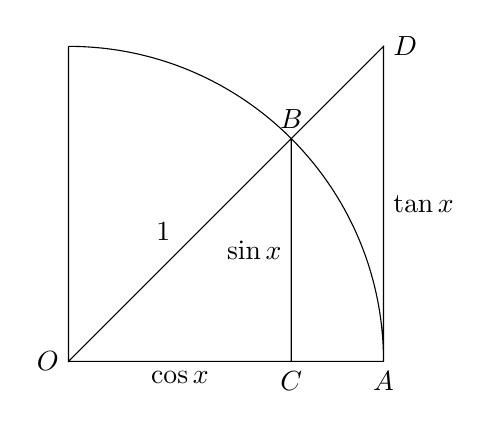
\begin{tikzpicture}
\pgfmathsetmacro{\r}{4}
\pgfmathsetmacro{\cx}{\r/sqrt(2)}
\coordinate (O) at (0,0);
\coordinate (A) at (\r,0);
\coordinate (B) at (\cx,\cx);
\coordinate (C) at (\cx,0);
\coordinate (D) at (\r,\r);
\draw (O)node[left]{\(O\)} -- (C)node[below]{\(C\)}node[midway,below]{\(\cos x\)} -- (A)node[below]{\(A\)}arc[start angle=0,end angle=90,radius=\r] (C) -- (B)node[above]{\(B\)}node[midway,left]{\(\sin x\)} -- (O)node[midway,above left]{\(1\)} -- (0,\r) (B) -- (D)node[right]{\(D\)} -- (A)node[midway,right]{\(\tan x\)};
\end{tikzpicture}
\end{center}
由于在\(0 < x < \pi/2\)时,\[
0 < \sin x < x < \tan x
\implies
1 < \frac{x}{\sin x} < \frac{1}{\cos x}
\implies
\cos x < \frac{\sin x}{x} < 1.
\]
因为\(\lim_{x\to0}\cos x = 1\),所以由\hyperref[theorem:极限.夹逼准则]{夹逼准则}可知,\(\lim_{x\to0} \frac{\sin x}{x} = 1\).
\end{proof}
\end{example}

\begin{figure}[ht]
	\centering
	\begin{tikzpicture}
		\begin{axis}[
			xmin=-4*pi,xmax=4*pi,
			ymin=-.5,ymax=1.2,
			width=\textwidth,
			height=.3\textheight,
			grid=both,
			xlabel=$x$,
			ylabel=$y$,
			enlargelimits,
			axis lines=middle,
			xtick={3.14,6.28,9.42,-3.14,-6.28,-9.42},
			xticklabels={$\pi$,$2\pi$,$3\pi$,$-\pi$,$-2\pi$,$-3\pi$},
		]
			\begin{scope}[samples=50,thick,red]
				\addplot[domain=.01:4*pi]{sin(deg(x))/x};
				\addplot[domain=-4*pi:-.01]{sin(deg(x))/x};
			\end{scope}
			\filldraw[draw=black,fill=white](0,1)circle(1pt);
		\end{axis}
	\end{tikzpicture}
	\caption{函数\(y=\frac{\sin x}{x}\)的图像}
	\label{figure:极限.函数[y=sin(x)/x]的图像}
\end{figure}

\begin{example}
\def\l{\lim_{x\to0}}
求:\(\l \frac{\tan x}{x}\).
\begin{solution}
\(
\l \frac{\tan x}{x}
= \l \left(\frac{\sin x}{x} \cdot \frac{1}{\cos x}\right)
= \l \frac{\sin x}{x} \cdot \lim_{x\to0}\frac{1}{\cos x}
= 1.
\)
\end{solution}
\end{example}

\begin{example}
\def\l{\lim_{x\to0}}
求:\(\l \frac{1 - \cos x}{x^2}\).
\begin{solution}
\(
\l \frac{1 - \cos x}{x^2}
= \l \frac{2 \sin^2\frac{x}{2}}{x^2}
= \frac{1}{2} \l \frac{\sin^2\frac{x}{2}}{\left(\frac{x}{2}\right)^2}
= \frac{1}{2} \left(\l \frac{\sin \frac{x}{2}}{\frac{x}{2}}\right)^2
= \frac{1}{2}.
\)
\end{solution}
\end{example}

\begin{example}
求:\(\lim_{x\to0}\frac{\arcsin x}{x}\).
\begin{solution}
令\(t = \arcsin x\),则\(x = \sin t\).当\(x\to0\)时,有\(t\to0\).于是由复合函数的极限运算法则得\[
\lim_{x\to0}\frac{\arcsin x}{x}
= \lim_{t\to0}\frac{t}{\sin t}
= 1.
\]
\end{solution}
\end{example}

\begin{example}
\def\l{\lim_{x\to0}}
计算\(\l \frac{\sin \omega x}{x}\).
\begin{solution}
当\(\omega=0\)时,\[
\l \frac{\sin \omega x}{x} = \l 0 = 0;
\]当\(\omega\neq0\)时,\[
\l \frac{\sin \omega x}{x}
= \omega \cdot \l \frac{\sin \omega x}{\omega x}
= \omega.
\]综上,\(\l \frac{\sin \omega x}{x} = \omega\).
\end{solution}
\end{example}

\begin{example}
\def\l{\lim_{x\to0}}
计算\(\l \frac{\sin mx}{\sin nx}\).
\begin{solution}
\(
\l \frac{\sin mx}{\sin nx}
= \frac{m}{n} \cdot \l \left( \frac{\sin mx}{mx} \cdot \frac{nx}{\sin nx} \right)
= \frac{m}{n}
\).
\end{solution}
\end{example}

\begin{example}
\def\l#1{\lim_{#1}}
计算\(\l{x\to\pi} \frac{\sin mx}{\sin nx} \quad(m,n\in\mathbb{Z})\).
\begin{solution}
\begin{align*}
\l{x\to\pi} \frac{\sin mx}{\sin nx}
&\xlongequal{t=x-\pi}
\l{t\to0} \frac{\sin m(t+\pi)}{\sin n(t+\pi)}
= \l{t\to0} \frac{(-1)^m}{(-1)^n} \frac{\sin mt}{\sin nt} \\
&= \l{t\to0} \frac{(-1)^m}{(-1)^n} \frac{\sin mt}{mt} \frac{m}{n} \frac{nt}{\sin nt}
= (-1)^{m-n} \frac{m}{n}.
\end{align*}
\end{solution}
\end{example}

\begin{example}
证明:\(\lim_{x\to0} \sqrt[n]{1+x} = 1\).
\begin{proof}
当\(x > 0\)时,
因为\(1 < \sqrt[n]{1+x} < 1+x\),
且\(\lim_{x\to0^+} 1 = \lim_{x\to0^+}(1+x) = 1\),
所以\[
	\lim_{x\to0^+} \sqrt[n]{1+x} = 1;
\]

当\(-1 < x < 0\)时,
因为\(1+x < \sqrt[n]{1+x} < 1\),
且\(\lim_{x\to0^-} 1 = \lim_{x\to0^-}(1+x) = 1\),
所以\[
	\lim_{x\to0^-} \sqrt[n]{1+x} = 1.
\]

综上,\(\lim_{x\to0} \sqrt[n]{1+x} = 1\).
\end{proof}
\end{example}

\begin{example}
证明:\(\lim_{x\to0^+} x \floor*{\frac{1}{x}} = 1\).
\begin{proof}
令\(t=1/x\),那么\[
x \floor*{\frac{1}{x}} = \frac{1}{t} \floor{t}.
\]又因为\[
t - 1 < \floor{t} \leq t,
\]\[
1 - \frac{1}{t} < \frac{1}{t} \floor{t} \leq 1;
\]而\[
\lim_{t\to+\infty} 1 - \frac{1}{t} = 1,
\quad
\lim_{t\to+\infty} 1 = 1,
\]所以\[
\lim_{x\to0^+} x \floor*{\frac{1}{x}} = \lim_{t\to+\infty} \frac{1}{t} \floor{t} = 1.
\qedhere
\]
\end{proof}
\end{example}


\subsection{单调有界定理}

相应于单调有界数列必有极限的准则,函数极限也有类似的准则.
\begin{theorem}\label{theorem:极限.函数的单调有界定理}
设函数\(f(x)\)在点\(x_0\)的某个左邻域\((x_0-\delta,x_0)\)内单调并且有界,则\(f(x)\)在\(x_0\)的左极限\(f(x_0^-)\)必定存在.
\end{theorem}

\begin{example}[重要极限II]
试证:极限\(\lim_{x \to \infty}\left(1 + \frac{1}{x}\right)^x\)存在.
\begin{proof}
考虑\(x\)取正整数\(n\)而趋于\(+\infty\)的情形.设\(x_n=\left(1+\frac{1}{n}\right)^n\),根据牛顿二项公式,有\begin{align*}
x_n &= \left(1+\frac{1}{n}\right)^n
= \sum_{k=0}^n \frac{n!}{k! (n-k)!} \frac{1}{n^k} \\
&= 1 + \frac{n}{1!}\frac{1}{n} + \frac{n(n-1)}{2!}\frac{1}{n^2} + \frac{n(n-1)(n-2)}{3!}\frac{1}{n^3} + \dotsb \\
&\qquad+ \frac{n(n-1)\dotsm(n-n+1)}{n!}\frac{1}{n^n} \\
&= 1 + 1 + \frac{1}{2!}\left(1-\frac{1}{n}\right) + \frac{1}{3!}\left(1-\frac{1}{n}\right)\left(1-\frac{2}{n}\right) + \dotsb \\
&\qquad+ \frac{1}{n!}\left(1-\frac{1}{n}\right)\left(1-\frac{2}{n}\right)\dotsm\left(1-\frac{n-1}{n}\right),
\end{align*}
类似地,\begin{align*}
x_{n+1}
&= 1 + 1 + \frac{1}{2!}\left(1-\frac{1}{n+1}\right) + \frac{1}{3!}\left(1-\frac{1}{n+1}\right)\left(1-\frac{2}{n+1}\right) + \dotsb \\
&\qquad+ \frac{1}{n!}\left(1-\frac{1}{n+1}\right)\left(1-\frac{2}{n+1}\right)\dotsm\left(1-\frac{n-1}{n+1}\right) \\
&\qquad+ \frac{1}{(n+1)!}\left(1-\frac{1}{n+1}\right)\left(1-\frac{2}{n+1}\right)\dotsm\left(1-\frac{n}{n+1}\right),
\end{align*}
比较\(x_n\)和\(x_{n+1}\)的展开式,可以看到除前两项外,\(x_n\)的每一项都小于\(x_{n+1}\)的对应项,并且\(x_{n+1}\)还多了最后一项\[
\frac{1}{(n+1)!}\left(1-\frac{1}{n+1}\right)\left(1-\frac{2}{n+1}\right)\dotsm\left(1-\frac{n}{n+1}\right) > 0,
\]因此\[
x_n < x_{n+1},
\]这就说明数列\(\{x_n\}\)是单调增加的.

又因为\[
x_n < 1 + 1 + \frac{1}{2!} + \frac{1}{3!} + \dotsb + \frac{1}{n!}
< 1 + 1 + \frac{1}{2} + \frac{1}{2^2} + \dotsb + \frac{1}{2^{n-1}}
= 3 - \frac{1}{2^{n-1}} < 3,
\]这就说明数列\(\{x_n\}\)是有界的.

既然数列\(\{x_n\}\)是单调增加的,
又是有界的,
那么数列\(\{x_n\}\)的极限一定存在,
记它的极限值为常数\(e\).

再设\(n \leq x < n+1\),则\[
\left(1+\frac{1}{n+1}\right)^n < \left(1+\frac{1}{x}\right)^x < \left(1+\frac{1}{n}\right)^{n+1},
\]且当\(n\to\infty\)时,\(x\to\infty\),而\[
\lim_{n\to\infty}\left(1+\frac{1}{n+1}\right)^n
=\lim_{n\to\infty}\frac{\left(1+\frac{1}{n+1}\right)^{n+1}}{1+\frac{1}{n+1}} = e,
\]\[
\lim_{n\to\infty}\left(1+\frac{1}{n}\right)^{n+1}
=\lim_{n\to\infty}\left[\left(1+\frac{1}{n}\right)^n\cdot\left(1+\frac{1}{n}\right)\right]=e,
\]应用\hyperref[theorem:极限.夹逼准则]{夹逼准则}可得\[
\lim_{x\to+\infty}\left(1+\frac{1}{x}\right)^x = e.
\]令\(x=-(t+1)\),则\(x\to-\infty\)时,\(t\to+\infty\),从而\begin{align*}
\lim_{x\to-\infty}\left(1+\frac{1}{x}\right)^x
&=\lim_{t\to+\infty}\left(1-\frac{1}{t+1}\right)^{-(t+1)}
=\lim_{t\to+\infty}\left(\frac{t}{t+1}\right)^{-(t+1)} \\
&=\lim_{t\to+\infty}\left(1+\frac{1}{t}\right)^{t+1}
=\lim_{t\to+\infty}\left[\left(1+\frac{1}{t}\right)^t\cdot\left(1+\frac{1}{t}\right)\right]=e.
\end{align*}

综上所述,由于\[
\lim_{x\to+\infty}\left(1+\frac{1}{x}\right)^x
= \lim_{x\to-\infty}\left(1+\frac{1}{x}\right)^x
= e,
\]所以\begin{equation}\label{equation:极限.重要极限II}
\lim_{x\to\infty} \left(1+\frac{1}{x}\right)^x = e.
\end{equation}
这就说明函数极限\(\lim_{x\to\infty} \left(1+\frac{1}{x}\right)^x\)存在.
\end{proof}
\end{example}
我们称上面所说的常数\(e\)为“\DefineConcept{欧拉常数} \(e\)”.

另外,利用复合函数的极限运算法则,可得
\begin{equation}
\lim_{z\to0}(1+z)^{\frac{1}{z}}
\xlongequal{z=1/x}
\lim_{x\to\infty}\left(1+\frac{1}{x}\right)^x
= e.
\end{equation}

\begin{figure}[ht]
	\centering
	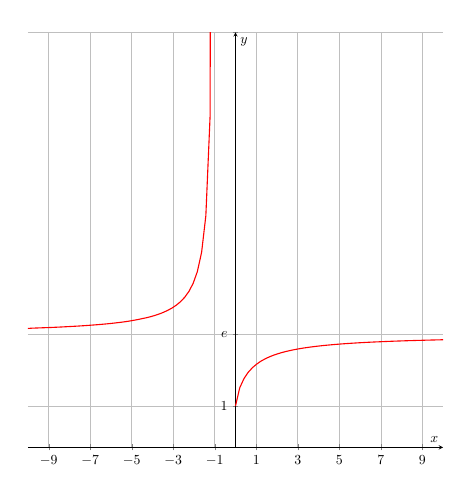
\begin{tikzpicture}[scale=.5]
	% Mathematica: Plot[{E,(1+1/x)^x},{x,-10,10},PlotRange->{0,10},AspectRatio->Automatic,PlotStyle->{{Dashed,Thin},Thin}]
		\begin{axis}[
			xmin=-10,xmax=10,ymin=0,ymax=10,
			grid=both,width=\textwidth,height=\textwidth,
			xlabel=$x$,
			ylabel=$y$,
			enlarge x limits=0.1,
			enlarge y limits=0.1,
			axis lines = middle,
			xtick={-9,-7,...,9},
			ytick={1,2.718,10},
			yticklabels={$1$,$e$},
		]
			\begin{scope}[samples=50,thick,red]
				\addplot[domain=-10:-0]{(1+1/x)^x};
				\addplot[domain=+0:+10]{(1+1/x)^x};
			\end{scope}
		\end{axis}
	\end{tikzpicture}
	\caption{函数\(y=\left(1+\tfrac{1}{x}\right)^x\)的图像}
	\label{figure:极限.函数(1+1/x)^x的图像}
\end{figure}

如\cref{figure:极限.函数(1+1/x)^x的图像} 所示,
我们可以画出函数\(y=\left(1+\frac{1}{x}\right)^x\ (x<-1 \lor x>0)\)的图像.
可见,直线\(y=e\)是函数\(y=\left(1+\frac{1}{x}\right)^x\)的图像的水平渐近线.
另外,易证\[
\lim_{x\to0^+} \left(1+\frac{1}{x}\right)^x = 1,
\qquad
\lim_{x\to1^-} \left(1+\frac{1}{x}\right)^x = +\infty.
\]


\begin{example}
求:\(\lim_{x \to \infty}\left(1 - \frac{1}{x}\right)^x\).
\begin{solution}
令\(t = -x\),则当\(x \to +\infty\)时,\(t \to -\infty\),于是\[
\lim_{x \to +\infty}\left(1 - \frac{1}{x}\right)^x
= \lim_{t \to -\infty}\left(1 + \frac{1}{t}\right)^{-t}
= \lim_{t \to -\infty}\frac{1}{\left(1 + \frac{1}{t}\right)^t}
= \frac{1}{e}.
\]
\end{solution}

画出函数\(y=\left(1-\frac{1}{x}\right)^x\ (x<0 \lor x\geq1)\)的图像如\cref{figure:极限.函数(1-1/x)^x的图像}.
\begin{figure}[ht]
	\centering
	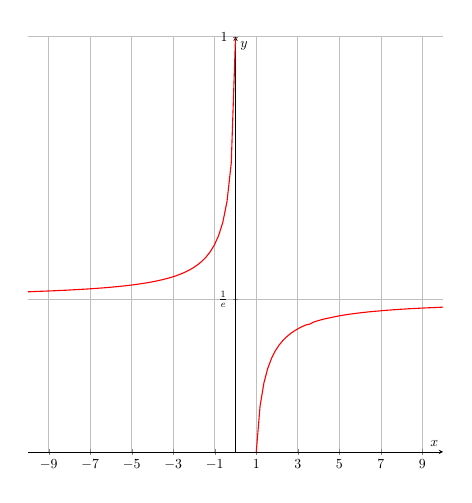
\begin{tikzpicture}[scale=.5]
		% Mathematica: Plot[{1/E, (1 - 1/x)^x}, {x, -10, 10}, PlotRange -> {0, 1}, PlotStyle -> {{Dashed, Thin}, Thin}]
		\begin{axis}[
			xmin=-10,xmax=10,
			ymin=0,ymax=1,
			grid=both,
			width=\textwidth,height=\textwidth,
			xlabel=$x$,
			ylabel=$y$,
			axis lines=middle,
			xtick={-9,-7,...,10},
			ytick={.3679,1},
			yticklabels={$\frac{1}{e}$,$1$},
		]
			\begin{scope}[samples=50,thick,red]
				\addplot[domain=-10:-0]{(1-1/x)^x};
				\addplot[domain=+1:+10]{(1-1/x)^x};
			\end{scope}
		\end{axis}
	\end{tikzpicture}
	\caption{函数\(y=\left(1-\tfrac{1}{x}\right)^x\)的图像}
	\label{figure:极限.函数(1-1/x)^x的图像}
\end{figure}
可见,直线\(y=\frac{1}{e}\)是函数\(y=\left(1-\frac{1}{x}\right)^x\)的图像的水平渐近线.
另外,易证\[
	\lim_{x\to0^-} \left(1-\frac{1}{x}\right)^x
	\xlongequal{t=-1/x} \lim_{t\to+\infty} \frac{1}{\sqrt[t]{1+t}}
	= 1.
\]
\end{example}

\subsection{柯西极限存在准则}

\begin{theorem}[柯西极限存在准则]\label{theorem:极限.数列的柯西极限存在准则}
%@see: 《高等数学(第六版 上册)》 P55 柯西极限存在准则
数列\(\{x_n\}\)收敛的充分必要条件是:
对于任意给定的正数\(\epsilon\),
存在正整数\(N\),
使得当\(m>N\)且\(n>N\)时,
就有\(\abs{x_n-x_m}<\epsilon\).
\begin{proof}
必要性.
设\(\lim_{n\to\infty}x_n = a\).
由数列极限的定义,
对于\(\forall\epsilon>0\),
\(\exists N \in \mathbb{N}^+\),
当\(n > N\)时,有\[
	\abs{x_n - a} < \frac{\epsilon}{2};
\]
同样地,当\(m > N\)时,有\[
	\abs{x_m - a} < \frac{\epsilon}{2}.
\]
因此,当\(n > N\)且\(m > N\)时,有\[
	\abs{x_n - x_m} = \abs{(x_n - a) - (x_m - a)}
	\leq \abs{x_n - a} + \abs{x_m - a}
	< \frac{\epsilon}{2} + \frac{\epsilon}{2}
	= \epsilon.
	\qedhere
\]
%TODO 未证充分性
\end{proof}
\end{theorem}
柯西极限存在准则有时也叫作\DefineConcept{柯西审敛原理}.

它可以用“\(\epsilon-\delta\)”语言表示为:\[
	\text{数列\(\{x_n\}\)收敛}
	\iff
	(\forall\epsilon>0)
	(\exists N\in\mathbb{N})
	(\forall n,m \geq N)
	[\abs{x_n-x_m}<\epsilon].
\]

类似地,函数极限也有自己的柯西审敛原理.

\begin{definition}\label{definition:极限.函数在集合上的振幅}
%@see: 《数学分析》(卓里奇) P109 定义16.
对于任意一个函数\(f\colon X\to\mathbb{R}\),
集合\(E \subseteq X\),
定义:\[
	\amp(f;E)
	\defeq
	\sup_{x_1,x_2 \in E}\abs{f(x_1)-f(x_2)},
\]
称为“函数\(f\)在集合\(E\)上的\DefineConcept{振幅}”.
\end{definition}

\begin{theorem}\label{theorem:极限.函数的柯西极限存在准则}
函数\(f(x)\)在点\(a\)的极限存在的充分必要条件是:
对于任意给定的正数\(\epsilon\),
存在正数\(\delta\),
使得当\(0 < \abs{x_1 - a} < \delta\)且\(0 < \abs{x_2 - a} < \delta\)时,
就有\(\abs{f(x_1) - f(x_2)} < \epsilon\).
\end{theorem}


\section{欧拉常数e}
可以证明,欧拉常数\(e\)是一个无理数,也是一个超越数,它的近似值约为2.718.

我们在前一节利用单调有界定理证明了数列极限\[
\lim_{n\to\infty} \left(1+\frac{1}{n}\right)^n = e,
\]
那么,当\(x\neq0\)时,有
\begin{align*}
	\lim_{n\to\infty} \left(1+\frac{x}{n}\right)^n
	&= \lim_{n\to\infty} \left(1+\frac{1}{n/x}\right)^{\frac{n}{x} \cdot x} \\
	&\xlongequal{t=n/x} \left[ \lim_{t\to\infty} \left(1+\frac{1}{t}\right)^t \right]^x
	= e^x;
\end{align*}
当\(x=0\)时,有\[
	\lim_{n\to\infty} \left(1+\frac{x}{n}\right)^n
	= \lim_{n\to\infty} (1+0)^n
	= \lim_{n\to\infty} 1
	= 1 \equiv e^0;
\]

我们可以得到一些关于自然对数的不等式.
\begin{gather}
	\frac{x}{1+x} < \ln(1+x) < x
	\quad(x>0), \\
	\frac{1}{n+1} < \ln(1+\frac{1}{n}) < \frac{1}{n}
	\quad(n\in\mathbb{N}^+), \\
	\ln(1+n) < \sum_{k=1}^n \frac{1}{k} < 1 + \ln n.
\end{gather}

\section{无穷小的比较}
在\cref{section:极限.极限的运算法则}中我们已经知道,
两个无穷小的和、差、积仍旧是无穷小.
但是,关于两个无穷小的商,却会出息不同的情况.
例如,当\(x\to0\)时,
\(3x\)、\(x^2\)、\(\sin x\)都是无穷小,
而\[
	\lim_{x\to0}\frac{x^2}{3x}=0, \qquad
	\lim_{x\to0}\frac{3x}{x^2}=\infty, \qquad
	\lim_{x\to0}\frac{\sin x}{3x}=\frac{1}{3}.
\]
两个无穷小之比的极限的各种不同情况,
反映了不同的无穷小趋于零的“快慢”程度.
就上面几个例子来说,
在\(x\to0\)的过程中,
\(x^2\to0\)比\(3x\to0\)要“快些”,
反过来说\(3x\to0\)比\(x^2\to0\)要“慢些”,
而\(\sin x\to0\)与\(x\to0\)“快慢相仿”.

下面,我们就无穷小之比的极限存在或为无穷大时,来说明两个无穷小之间的比较.
应当注意,下面的\(\alpha\)及\(\beta\)都是在同一个自变量的变化过程中的无穷小,
且\(\alpha\neq0\),\(\lim\frac{\beta}{\alpha}\)也是在这个变化过程中的极限.

应该注意到,记号\(o(\alpha)\)实际上是由所有满足\[
\lim \frac{\beta}{\alpha} = 0
\]的函数\(\beta\)构成的集合,即\[
o(\alpha) = \Set*{ \beta \given \lim \frac{\beta}{\alpha} = 0 }.
\]虽然在给定\(\lim \frac{\beta}{\alpha}\)时,我们本该用记号\(\beta \in o(\alpha)\)表示\(\beta\)是比\(\alpha\)高阶的无穷小,但我们在后面很快就会看到使用记号\(\beta = o(\alpha)\)的诸多好处.

\begin{example}
因为\(\lim_{x\to0} \frac{3x^2}{x} = 0\),所以当\(x\to0\)时,\(3x^2\)是比\(x\)高阶的无穷小,即\(3x^2 = o(x)\ (x\to0)\).

因为\(\lim_{n\to\infty} \frac{1/n}{1/n^2} = \infty\),所以当\(n\to\infty\)时,\(\frac{1}{n}\)是比\(\frac{1}{n^2}\)低阶的无穷小.

因为\(\lim_{x\to3} \frac{x^2-9}{x-3} = 6\),所以当\(x\to3\)时,\(x^2-9\)与\(x-3\)是同阶无穷小.

因为\(\lim_{x\to0} \frac{1-\cos x}{x^2} = \frac{1}{2}\),所以当\(x\to0\)时,\(1-\cos x\)是关于\(x\)的二阶无穷小.

因为\(\lim_{x\to0} \frac{\sin x}{x} = 1\),所以当\(x\to0\)时,\(\sin x\)与\(x\)是等价无穷小,即\(\sin x \sim x\ (x\to0)\).
\end{example}

\begin{example}
%@see: 《高等数学(第六版 上册)》 P58 例1
证明:当\(x\to0\)时,\(\sqrt[n]{1+x} - 1 \sim \frac{1}{n} x\).
\begin{proof}
因为\begin{align*}
\frac{\sqrt[n]{1+x} - 1}{\frac{1}{n} x}
&= \frac{(\sqrt[n]{1+x})^n - 1}{\frac{1}{n} x \left[ \sqrt[n]{(1+x)^{n-1}} + \sqrt[n]{(1+x)^{n-2}} + \dotsb + 1 \right]} \\
&= \frac{n}{\sqrt[n]{(1+x)^{n-1}} + \sqrt[n]{(1+x)^{n-2}} + \dotsb + 1},
\end{align*}
而\[
\lim_{x\to0} \sqrt[n]{(1+x)^m} = 1,
\]所以\[
\lim_{x\to0} \frac{\sqrt[n]{1+x} - 1}{\frac{1}{n} x} = \lim_{x\to0} \frac{n}{1 \cdot n} = 1,
\]也就是说\(\sqrt[n]{1+x} - 1 \sim \frac{1}{n} x \quad(x\to0)\).
\end{proof}
\end{example}

\begin{theorem}\label{theorem:极限.无穷小的比较1}
%@see: 《高等数学(第六版 上册)》 P58 定理1
\(\beta\)与\(\alpha\)是等价无穷小的充分必要条件为\[
	\beta=\alpha+o(\alpha).
\]
\begin{proof}
必要性.
设\(\alpha\sim\beta\),则\[
	\lim\frac{\beta-\alpha}{\alpha}
	=\lim\left(\frac{\beta}{\alpha}-1\right)
	=\lim\frac{\beta}{\alpha}-1 = 0,
\]
因此\(\beta-\alpha=o(\alpha)\),即\(\beta=\alpha+o(\alpha)\).

充分性.
设\(\beta=\alpha+o(\alpha)\),则\[
	\lim\frac{\beta}{\alpha}
	=\lim\frac{\alpha+o(\alpha)}{\alpha}
	=\lim\left(1+\frac{o(\alpha)}{\alpha}\right) = 1,
\]
因此\(\alpha\sim\beta\).
\end{proof}
\end{theorem}

\begin{theorem}\label{theorem:极限.无穷小的比较2}
%@see: 《高等数学(第六版 上册)》 P59 定理2
设\(\alpha\sim\alpha'\),\(\beta\sim\beta'\),
且\(\lim\frac{\beta'}{\alpha'}\)存在,
则\[
	\lim\frac{\beta}{\alpha}=\lim\frac{\beta'}{\alpha'}.
\]
\begin{proof}
由\(\alpha\sim\alpha'\)和\(\beta\sim\beta'\)有
\(\lim\frac{\alpha'}{\alpha} = 1\),
\(\lim\frac{\beta}{\beta'} = 1\),
因此\[
	\lim\frac{\beta}{\alpha}
	= \lim \left(
		\frac{\beta}{\beta'}
		\cdot \frac{\beta'}{\alpha'}
		\cdot \frac{\alpha'}{\alpha}
	\right)
	= \lim\frac{\beta}{\beta'}
		\cdot \lim \frac{\beta'}{\alpha'}
		\cdot \lim\frac{\alpha'}{\alpha}
	= 1 \cdot \lim \frac{\beta'}{\alpha'} \cdot 1
	= \lim \frac{\beta'}{\alpha'}.
	\qedhere
\]
\end{proof}
\end{theorem}
\cref{theorem:极限.无穷小的比较2} 表明,
求两个无穷小之比的极限时,
分子及分母都可用等价无穷小来代替.
因此,如果用来代替的无穷小选得适当的话,
可以使计算简化.

必须指出的是,等价无穷小实际上是一种等价关系.
\begin{property}\label{theorem:极限.无穷小的比较6}
设\(\alpha,\beta,\gamma\)都是在同一个自变量的变化过程中的无穷小,
那么\begin{enumerate}
	\item {\bf 自反性}:
	\(\alpha \sim \alpha\);

	\item {\bf 对称性}:
	\(\alpha \sim \beta \implies \beta \sim \alpha\);

	\item {\bf 传递性}:
	\(\alpha \sim \beta, \beta \sim \gamma \implies \alpha \sim \gamma\).
\end{enumerate}
\end{property}


\begin{proposition}
设\(\alpha,\beta,\gamma\)都是在同一个自变量的变化过程中的无穷小,
\(\alpha\neq0,
\gamma\neq0\),
且\[
	\lim\frac{\beta}{\alpha^p}=c_1\in(0,+\infty), \qquad
	\lim\frac{\gamma}{\alpha^q}=c_2\in(0,+\infty).
\]
那么:\begin{enumerate}
	\item 若\(p>q\),
	则\(\beta\)是比\(\gamma\)高阶的无穷小.

	\item 若\(p=q\),
	则\(\beta\)是比\(\gamma\)同阶的无穷小.

	\item 若\(p<q\),
	则\(\beta\)是比\(\gamma\)低阶的无穷小.
\end{enumerate}

\begin{proof}
容易得到\begin{align*}
	\lim\frac{\beta}{\gamma}
	&= \lim\left(
			\frac{\beta}{\alpha^p}
			\frac{\alpha^p}{\alpha^q}
			\frac{\alpha^q}{\gamma}
		\right) \\
	&= \lim\frac{\beta}{\alpha^p}
		\cdot \lim\frac{\alpha^p}{\alpha^q}
		\cdot \lim\frac{\alpha^q}{\gamma} \\
	&= c_1 \cdot \lim\alpha^{p-q} \cdot c_2^{-1}
	= \frac{c_1}{c_2} \lim\alpha^{p-q}.
	\tag1
\end{align*}
注意到\(\lim\alpha=0\).
当\(p>q\)时,(1)式等于\(0\),\(\beta\)是比\(\gamma\)高阶的无穷小,即\(\beta=o(\gamma)\).
当\(p=q\)时,(1)式等于\(\frac{c_1}{c_2}\),\(\beta\)是比\(\gamma\)同阶的无穷小.
当\(p<q\)时,(1)式等于\(\infty\),\(\beta\)是比\(\gamma\)低阶的无穷小,即\(\gamma=o(\beta)\).
\end{proof}
\end{proposition}
正因如此,我们常在求极限的时候,将某个数列或函数作为比较无穷小的阶的参照系.
例如,在讨论当\(n\to\infty\)时的无穷小时,
我们把数列\(\left\{\frac1n\right\}\)作为参照系,
计算极限\(\lim_{n\to\infty} n \sin\frac1n = 1\),
然后说“数列\(\left\{\sin\frac1n\right\}\)是(\(\frac1n\)的)1阶无穷小”.
又例如,在讨论当\(x\to0\)时的无穷小时,
我们把函数\(f(x)=x\)作为参考系,
计算极限\(\lim_{x\to0} \frac{3x^2+4x^5}{x^2} = 3\),
然后说“函数\(3x^2+4x^5\)是(\(x\)的)2阶无穷小”.

\begin{proposition}[和差取大规则]\label{theorem:极限.无穷小的比较3}
设\(\beta=o(\alpha)\),则\(\alpha\pm\beta\sim\alpha\).
\end{proposition}
\cref{theorem:极限.无穷小的比较3} 说明,
当高阶无穷小\(\beta\)和低阶无穷小\(\alpha\)相加或相减时,
它们的等价无穷小就是低阶无穷小\(\alpha\).
因为当自变量变化时,高阶无穷小比低阶无穷小更快地趋于零,
相对而言,低阶无穷小就显得更“大”一些,
因此我们把\cref{theorem:极限.无穷小的比较3} 称为“和差取大规则”.

\begin{proposition}[和差代替规则]\label{theorem:极限.无穷小的比较4}
设\(\alpha\sim\alpha'\),\(\beta\sim\beta'\),\(\beta\)与\(\alpha\)不是等价无穷小,则\[
	\alpha\pm\beta\sim\alpha'\pm\beta'.
\]
\end{proposition}

\begin{proposition}[因式代替规则]\label{theorem:极限.无穷小的比较5}
设\(\alpha\sim\beta\),且函数\(\phi\)有界或\(\lim\phi\)存在,则\[
	\alpha \phi \sim \beta \phi.
\]
\end{proposition}

\section{施托尔茨定理}
\begin{theorem}[施托尔茨定理I]\label{theorem:极限.施托尔茨定理1}
%@see: 《数学分析(第二版 上册)》(陈纪修) P49 定理2.3.3
设数列\(\{x_n\},\{y_n\}\).
若\(\{y_n\}\)是严格单调增加的正无穷大,
且\[
	\lim_{n\to\infty} \frac{x_{n+1}-x_n}{y_{n+1}-y_n}
	= C
	\in[-\infty,+\infty],
\]
那么有\[
	\lim_{n\to\infty} \frac{x_n}{y_n}
	= C.
\]
% \begin{proof}%TODO
% 设\(\lim_{n\to\infty} \frac{x_{n+1}-x_n}{y_{n+1}-y_n} = C\in(-\infty,+\infty)\),
% 故对\(\forall\epsilon>0\),\(\exists N>0\),当\(n > N\)时,有\[
% \abs{\frac{x_{n+1}-x_n}{y_{n+1}-y_n} - C} < \epsilon
% \]成立,即\[
% C - \epsilon < \frac{x_{n+1}-x_n}{y_{n+1}-y_n} < C + \epsilon;
% \]
% 由于\[
% \frac{
% (x_{N+1}-x_N)
% + (x_{N+2}-x_{N+1})
% + \dotsb
% + (x_{n+1}-x_n)
% }{
% (y_{N+1}-y_N)
% + (y_{N+2}-y_{N+1})
% + \dotsb
% + (y_{n+1}-y_n)
% }
% = \frac{x_{n+1}-x_N}{y_{n+1}-y_N},
% \]再根据\cref{example:不等式.不同浓度的溶液的混合},于是有\[
% C - \epsilon <
% \frac{x_{n+1}-x_N}{y_{n+1}-y_N}
% < C + \epsilon;
% \]进而有\[
% \lim_{n\to\infty} \frac{x_{n+1}-x_N}{y_{n+1}-y_N}
% = \lim_{n\to\infty} \frac{\frac{x_{n+1}}{y_{n+1}}-\frac{x_N}{y_{n+1}}}{1-\frac{y_N}{y_{n+1}}}
% = C;
% \]又因为\(\lim_{n\to\infty} y_n = +\infty\),
% 注意到\(x_N\)、\(y_N\)是不随\(n\)变化的常数,
% 于是有\(\lim_{n\to\infty} \frac{x_N}{y_{n+1}}
% = \lim_{n\to\infty} \frac{y_N}{y_{n+1}}
% = 0\),从而有\(\lim_{n\to\infty} \frac{x_{n+1}}{y_{n+1}} = C\).
% \end{proof}
\end{theorem}

\begin{theorem}[施托尔茨定理II]\label{theorem:极限.施托尔茨定理2}
设数列\(\{x_n\},\{y_n\}\).
若\(\{x_n\}\)是无穷小,
\(\{y_n\}\)是严格单调减少的无穷小,且\[
	\lim_{n\to\infty} \frac{x_{n+1}-x_n}{y_{n+1}-y_n}
	= C
	\in[-\infty,+\infty],
\]
那么有\[
	\lim_{n\to\infty} \frac{x_n}{y_n}
	= C.
\]
\end{theorem}

% 施托尔茨定理实际上是离散形式的洛必达法则,它适用于\(\frac{0}{0}\)、\(\frac{\infty}{\infty}\)或\(\frac{*}{\infty}\)三种情形.

\begin{example}
%@see: 《数学分析(第二版 上册)》(陈纪修) P50
利用施托尔茨定理重新证明\cref{example:极限.数列的算术平均的极限}.
\begin{proof}
令\(x_n=a_1+a_2+\dotsb+a_n,y_n=n\),
由\cref{theorem:极限.施托尔茨定理1} 有\[
	\lim_{n\to\infty} \frac{x_n}{y_n}
	= \lim_{n\to\infty} \frac{x_{n+1}-x_n}{y_{n+1}-y_n}
	= \lim_{n\to\infty} \frac{a_{n+1}}{1}
	= a.
	\qedhere
\]
\end{proof}
\end{example}

\begin{example}
%@see: 《数学分析(第二版 上册)》(陈纪修) P50 例2.3.4
设\(p>-1\).
证明:\begin{equation}\label{equation:数列极限.重要极限X}
	\lim_{n\to\infty} \frac{1^p+2^p+\dotsb+n^p}{n^{p+1}}
	= \frac{1}{p+1}.
\end{equation}
\begin{proof}
令\(x_n=1^p+2^p+\dotsb+n^p,
y_n=n^{p+1}\),
由\cref{theorem:极限.施托尔茨定理1} 有\begin{align*}
	\lim_{n\to\infty} \frac{x_n}{y_n}
	&= \lim_{n\to\infty} \frac{x_{n+1}-x_n}{y_{n+1}-y_n}
	= \lim_{n\to\infty} \frac{(n+1)^p}{(n+1)^{p+1} - n^{p+1}} \\
	&= \lim_{n\to\infty} \frac{n^p + p n^{p-1} + \dotsb + 1}
		{(p+1) n^p + \frac{1}{2} (p+1) p n^{p-1} + \dotsb + 1} \\
	&= \frac{1}{p+1}.
	\qedhere
\end{align*}
\end{proof}
\end{example}

\begin{example}
%@see: 《数学分析(第二版 上册)》(陈纪修) P50 例2.3.5
设\(\lim_{n\to\infty} a_n = a\),
求极限\(\lim_{n\to\infty} \frac{a_1+2a_2+\dotsb+na_n}{n^2}\).
\begin{solution}
令\(x_n=a_1+2a_2+\dotsb+na_n,
y_n=n^2\),
由\cref{theorem:极限.施托尔茨定理1} 有\[
	\lim_{n\to\infty} \frac{x_n}{y_n}
	= \lim_{n\to\infty} \frac{x_{n+1}-x_n}{y_{n+1}-y_n}
	= \lim_{n\to\infty} \frac{(n+1)a_{n+1}}{(n+1)^2-n^2}
	= \lim_{n\to\infty} \frac{(n+1)a_{n+1}}{2n+1}
	= \frac12 a.
\]
\end{solution}
\end{example}

设变量\(u\)从它的一个初值\(u_1\)变到终值\(u_2\),
终值与初值的差\(u_2 - u_1\)就叫做变量\(u\)的\DefineConcept{增量},
记作\(\increment u\),即\[
	\increment u = u_2 - u_1.
\]

在实数域中,增量\(\increment u\)既可以是正的,也可以是负的.
当\(\increment u > 0\)时,变量\(u\)从初值变到终值时是增大的;
当\(\increment u < 0\)时,变量\(u\)从初值变到终值时是减小的.

应该注意到:
记号\(\increment u\)并不表示某个量\(\Delta\)与变量\(u\)的乘积,
而是一个不可分割的符号.

%\subsection{连续曲线}
%\begin{definition}
%设平面曲线\(L\)的参数方程为\[
%	\left\{ \begin{array}{l}
%		x = \phi(t) \\
%		y = \psi(t)
%	\end{array} \right.,
%	\quad
%	t \in [\alpha,\beta].
%\]
%如果\(\phi(t)\)、\(\psi(t)\)在\([\alpha,\beta]\)上连续,
%则称曲线\(L\)为\DefineConcept{连续曲线}.
%点\(\opair{\phi(\alpha),\psi(\alpha)}\)称为曲线的\DefineConcept{起点},
%点\(\opair{\phi(\beta),\psi(\beta)}\)称为曲线的\DefineConcept{终点}.
%
%如果存在\(t_1\)、\(t_2\)满足\(\alpha \leq t_1 < t_2 \leq \beta\)
%且\((t_1-\alpha)^2+(t_2-\beta)^2 \neq 0\),使得对应的两点重合,
%即\(\opair{\phi(t_1),\psi(t_1)}=\opair{\phi(t_2),\psi(t_2)}\)成立,
%则称该点为曲线\(L\)的\DefineConcept{重点}.
%
%无重点的连续曲线称为\DefineConcept{若尔当曲线}或\DefineConcept{简单曲线}.
%
%仅起点和终点重合
%(即\(\opair{\phi(\alpha),\psi(\alpha)}
%=\opair{\phi(\beta),\psi(\beta)}\))
%的简单曲线称作\DefineConcept{若尔当闭曲线}或者\DefineConcept{简单闭曲线}.
%\end{definition}

\section{连续函数的运算与初等函数的连续性}
\subsection{连续函数的和、差、积、商的连续性}

\subsection{反函数与复合函数的连续性}

\subsection{初等函数的连续性}
\begin{theorem}\label{theorem:极限.连续函数的极限5}
基本初等函数在其定义域内都是连续的.
\end{theorem}

\begin{corollary}\label{theorem:极限.连续函数的极限6}
一切初等函数在其定义区间(即包含在定义域内的区间)内都是连续的.
\end{corollary}

\begin{example}
求:\(\lim_{x\to0}\frac{\log_a (1+x)}{x}\).
\begin{solution}
\(
\lim_{x\to0}\frac{\log_a (1+x)}{x}
= \lim_{x\to0}\log_a (1+x)^{\frac{1}{x}}
= \log_a \lim_{x\to0}(1+x)^{\frac{1}{x}}
= \log_a e
= \frac{1}{\ln a}.
\)
\end{solution}
\end{example}

\begin{example}
求:\(\lim_{x\to0}\frac{a^x - 1}{x}\).
\begin{solution}
\(
\lim_{x\to0}\frac{a^x - 1}{x}
\xlongequal{t=a^x-1} \lim_{t\to0}\frac{t}{\log_a (1+t)}
= \ln a.
\)
\end{solution}
\end{example}

\begin{proposition}
%@see: 《高等数学(第六版 上册)》 P69 习题1-9 2.
设函数\(f(x)\)和\(g(x)\)在点\(x_0\)连续,
则\[
	\phi(x)=\max\{f(x),g(x)\}, \qquad
	\psi(x)=\min\{f(x),g(x)\}
\]在点\(x_0\)也连续.
\begin{proof}
因为\[
	\phi(x)=\frac{f(x)+g(x)}{2}+\frac{\abs{f(x)-g(x)}}{2}, \qquad
	\psi(x)=\frac{f(x)+g(x)}{2}-\frac{\abs{f(x)-g(x)}}{2},
\]
所以\(\phi(x)\)和\(\psi(x)\)在点\(x_0\)也连续.
\end{proof}
\end{proposition}

\begin{theorem}\label{theorem:极限.连续函数的极限7}
对于幂指函数\(y = u(x)^{v(x)}\ (u(x) > 0\)且\(u(x) \not\equiv 1)\),如果\(\lim u(x) = a > 0\),\(\lim v(x) = b\),那么\[
\lim u(x)^{v(x)} = a^b.
\]
\end{theorem}

\begin{example}
\def\l{\lim_{n\to\infty}}
计算:\(\l \sin^2(\pi\sqrt{n^2+3n})\).
\begin{solution}
\def\a{\pi(\sqrt{n^2+3n}-\sqrt{n^2})}
显然有\begin{align*}
&\l \sin^2(\pi\sqrt{n^2+3n}) \\
&= \l \sin^2[n\pi+\a] \\
&= \l \left\{ \sin(n\pi) \cos\left[\a\right] + \cos(n\pi) \sin\left[\a\right] \right\}^2 \\
&= \l \sin^2\left[\a\right] \\
&= \l \sin^2\left( \pi \cdot \frac{3n}{\sqrt{n^2+3n}+n} \right) \\
&= \sin^2 \left( \pi \cdot \l \frac{3n}{\sqrt{n^2+3n}+n} \right) \\
&= \sin^2 \frac{3\pi}{2}
= 1.
\end{align*}
\end{solution}
\end{example}

\begin{example}
设\(x_1=10\),\(x_{n+1}=\sqrt{6+x_n}\ (n=1,2,\dotsc)\).
试证:数列\(\{x_n\}\)极限存在,并求此极限.
\begin{solution}
由\(x_1=10\),
\(x_2=\sqrt{6+x_1}=\sqrt{16}=4\),
可知\(x_1>x_2\).
因此我们猜想数列\(\{x_n\}\)是单调递减数列.
假设\(n=k\)时有\(x_k>x_{k+1}\)成立,
那么\[
	x_{k+1}=\sqrt{6+x_k}>\sqrt{6+x_{k+1}}=x_{k+2},
\]
所以利用数学归纳法便知\(x_n>x_{n+1}\ (n=1,2,\dotsc)\).

同理,由于\(x_{n+1}=\sqrt{6+x_n}\),
所以利用数学归纳法便知\(x_n>0\ (n=1,2,\dotsc)\).

根据\hyperref[theorem:极限.数列的单调有界定理]{单调有界定理},
数列\(\{x_n\}\)有极限.

设\(\lim_{n\to\infty}x_n=x\).
对\(x_{n+1}=\sqrt{6+x_n}\)两边取极限,
得\[
	\lim_{n\to\infty}x_{n+1}=x, \qquad
	\lim_{n\to\infty}\sqrt{6+x_n}
	=\sqrt{6+\lim_{n\to\infty}x_n}
	=\sqrt{6+x},
\]
于是\(x=\sqrt{6+x}\),
从而\(x^2-x-6=0\),
\((x-3)(x+2)=0\),
解得\(x=3\)或\(x=-2\)(舍去).
这就是说\(\lim_{n\to\infty}x_n=3\).
\end{solution}
\end{example}

\section{闭区间上连续函数的性质}
在\cref{section:极限.函数的连续性与间断点}中已说明了函数在区间上连续的概念,
在闭区间上连续的函数有几个重要的性质,下面予以叙述.

\subsection{有界性与最大值最小值定理}
\begin{definition}
函数\(f(x)\)在区间\(I\)上有定义.

如果有\(x_0 \in I\),使得对于任一\(x \in I\)都有\[
	f(x) \leq f(x_0),
\]
则称“\(f(x_0)\)是函数\(f(x)\)在区间\(I\)上的\DefineConcept{最大值}”,
记作\(\max_{x \in I}f(x) = f(x_0)\).

如果有\(x_0 \in I\),使得对于任一\(x \in I\)都有\[
	f(x) \geq f(x_0),
\]
则称“\(f(x_0)\)是函数\(f(x)\)在区间\(I\)上的\DefineConcept{最小值}”,
记作\(\min_{x \in I}f(x) = f(x_0)\).
\end{definition}

\begin{theorem}[有界性与最大值最小值定理]\label{theorem:极限.最值定理}
在闭区间上连续的函数在该区间上有界且一定能取得它的最大值和最小值.
\begin{proof}
用反证法.
假设连续函数\(f\)在闭区间\([a,b]\)上无界,
那么根据\hyperref[definition:函数.函数的有界性]{有界函数的定义}可知\[
	(\forall M>0)
	(\exists x_n\in[a,b])
	[\abs{f(x_n)} > M],
\]
换言之,函数列\(\{f(x_n)\}\)满足\[
	\lim_{n\to\infty} f(x_n) = \infty;
\]
但是数列\(\{x_n\}\)有界(即\(a \leq x_n \leq b\)),
因此在闭区间\([a,b]\)内存在收敛子列\(\{x_{n_k}\}\),
不妨设\[
	\lim_{k\to\infty} x_{n_k} = c \in [a,b];
\]
然而根据函数\(f\)的连续性可知,\[
	f(c) = \lim_{k\to\infty} f(x_{n_k}),
\]
这就和\(f(x_n)\to\infty\ (n\to\infty)\)矛盾,因此函数\(f\)在\([a,b]\)上有界.
\end{proof}
\end{theorem}
我们也把\hyperref[theorem:极限.最值定理]{有界性与最大值最小值定理}称为%
\DefineConcept{魏尔斯特拉斯最值定理}.

注意:如果函数在开区间内连续,或函数在闭区间上有间断点,
那么函数在该区间上不一定有界,也不一定有最大值或最小值.

如果函数在开区间内连续,
或者函数在闭区间上有间断点,
那么这个函数在该区间上不一定有解,
也不一定有最大值或最小值.
例如,函数\(y=\tan x\)在开区间\(\left(-\frac{\pi}{2},\frac{\pi}{2}\right)\)内是连续的,
但它在\(\left(-\frac{\pi}{2},\frac{\pi}{2}\right)\)内是无界的,
且既无最大值又无最小值;
又如,函数\[
	y=\left\{ \begin{array}{ll}
		1-x, & 0\leq x<1, \\
		1, & x=1, \\
		3-x, & 1<x\leq2
	\end{array} \right.
\]在闭区间\([0,2]\)上间断点\(x=1\),
它在闭区间\([0,2]\)上虽然有界,
但是既无最大值又无最小值.

\subsection{零点定理与介值定理}
\begin{definition}
如果\(x_0\)使\(f(x_0) = 0\),则\(x_0\)称为函数\(f(x)\)的\DefineConcept{零点}.
\end{definition}

\begin{theorem}[零点定理]\label{theorem:极限.零点定理}
设函数\(f(x)\)在闭区间\([a,b]\)上连续,
且\(f(a) \cdot f(b)<0\),
那么\[
	(\exists\xi\in(a,b))[f(\xi) = 0].
\]
\begin{proof}
用反证法.
假设对\(\forall x\in(a,b)\)都有\(f(x) \neq 0\).

因为\(f(a) \cdot f(b)<0\),
不妨设\(f(a) < 0 < f(b)\).
若\(f\left(\frac{a+b}{2}\right)>0\),取\(a_1=a\)、\(b_1=\frac{a+b}{2}\);
若\(f\left(\frac{a+b}{2}\right)<0\),取\(a_1=\frac{a+b}{2}\)、\(b_1=b\);
总之,在上述两种情形下均有不等式\(f(a_1) < 0 < f(b_1)\)成立.
以此类推,建立闭区间序列\(\{[a_n,b_n]\}\),
可知\[
[a_{n+1},b_{n+1}] \subseteq [a_n,b_n],
f(a_n) < 0 < f(b_n),
\lim_{n\to\infty} (b_n - a_n)
= \lim_{n\to\infty} \frac{b-a}{2^n}
= 0.
\]
根据\cref{definition:极限.闭区间套定理},
\(\exists\xi\in[a,b]\)满足\(\lim_{n\to\infty} a_n
= \xi
= \lim_{n\to\infty} b_n\).

由\hyperref[theorem:极限.函数极限的局部保号性3]{函数极限的局部保号性}有\[
\lim_{n\to\infty} f(a_n) \leq 0,
\qquad
\lim_{n\to\infty} f(b_n) \geq 0.
\]
又因为\(f \in C[a,b]\),由连续函数的定义可知,\(\lim_{x\to\xi} f(x) = f(\xi)\);
那么由\hyperref[theorem:极限.海涅定理]{海涅定理}可知,\[
\lim_{n\to\infty} f(a_n)
= \lim_{n\to\infty} f(b_n)
= f(\xi).
\]再由\hyperref[theorem:极限.夹逼准则]{夹逼准则}有\(f(\xi)=0\).
\end{proof}
\end{theorem}
我们也把\hyperref[theorem:极限.零点定理]{零点定理}称为%
\DefineConcept{波尔查诺--柯西中值定理}.

从几何上看,零点定理表示:
如果连续曲线弧\(y = f(x)\)的两个端点位于\(x\)轴的不同侧,那么这段曲线弧与\(x\)轴至少有一个交点.

\begin{theorem}[介值定理]\label{theorem:极限.闭区间上连续函数的性质.介值定理1}
%@see: 《高等数学(第六版 上册)》 P72 定理3
设函数\(f(x)\)在闭区间\([a,b]\)上连续,且在这区间的端点取不同的函数值\[
	f(a) = A
	\quad\text{及}\quad
	f(b) = B.
\]
那么,对于\(A\)与\(B\)之间的任意一个数\(C\),
在开区间\((a,b)\)内至少有一个点\(\xi\),使得\[
	f(\xi)=C
	\quad(a<\xi<b).
\]
\begin{proof}
设\(\phi(x)=f(x)-C\),
则\(\phi(x)\)在闭区间\([a,b]\)上连续,
且\(\phi(a)=A-C\)与\(\phi(b)=B-C\)异号.
根据零点定理,开区间\((a,b)\)内至少有一点\(\xi\)使得\[
	\phi(\xi)=0
	\quad(a<\xi<b).
\]
又\(\phi(\xi)=f(\xi)-C\),
因此由上式即得\[
	f(\xi)=C
	\quad(a<\xi<b).
	\qedhere
\]
\end{proof}
\end{theorem}
\cref{theorem:极限.闭区间上连续函数的性质.介值定理1} 的几何意义是:
连续曲线弧\(y=f(x)\)与水平直线\(y=C\)至少相交于一点.

\begin{corollary}\label{theorem:极限.闭区间上连续函数的性质.介值定理2}
%@see: 《高等数学(第六版 上册)》 P72 推论
在闭区间上连续的函数必取得介于最大值\(M\)与最小值\(m\)之间的任何值.
\begin{proof}
设函数\(f \in C[a,b]\),取\[
	M=\max_{a \leq x \leq b} f(x), \qquad
	m=\min_{a \leq x \leq b} f(x),
\]
假设\(m=f(x_1)\),\(M=f(x_2)\),且\(m \neq M\),\(x_1 \neq x_2\).
在闭区间\([\min\{x_1,x_2\},\max\{x_1,x_2\}]\)上应用介值定理,
于是有\[
	(\forall\mu\in(m,M))(\exists\xi\in(a,b))
	[f(\xi)=\mu].
	\qedhere
\]
\end{proof}
\end{corollary}

\begin{corollary}
如果\(I\)是区间,且\(f\in C(I)\),则\(f\ImageOfSetUnderRelation{I}\)也是区间.
\end{corollary}

\begin{corollary}
设函数\(f\)是定义在区间\(I\)上的严格单调函数,
则\(f\)连续当且仅当\(f\ImageOfSetUnderRelation{I}\)也是区间.
\end{corollary}

\begin{corollary}
定义在区间\(I\)上的严格单调连续函数必然可逆,且逆函数也是严格单调连续的.
\end{corollary}

\begin{corollary}
如果\(f \in C(I)\),则\(f\)严格单调当且仅当\(f^{-1}\)存在.
\end{corollary}

\begin{corollary}
如果\(f\colon[a,b]\to[a,b]\)连续,则\(\exists\xi\in[a,b]: f(\xi)=\xi\).
\end{corollary}

\begin{example}
设\(f \in C[a,b]\),证明:函数\[
m(x) = \inf_{a \leq y \leq x} f(y), \qquad
M(x) = \sup_{a \leq y \leq x} f(y)
\]都在\([a,b]\)上连续.
\begin{proof}
这里只证\(m\)是连续的.
\begin{enumerate}
\item 首先证明\(m\)在点\(x=a\)处右连续.
注意到\(m(a) = f(a)\).
对\(\forall\epsilon>0\),由于\(f\)在\(x=a\)处右连续,所以\(\exists\delta>0\)使得对\(\forall x\in(a,a+\delta)\)都有\(\abs{f(x)-f(a)}<\epsilon\)成立;
因此\[
f(x)
> f(a) - \epsilon
= m(a) - \epsilon.
\]
于是,当\(x\in[a,a+\delta)\)时,对\(\forall y\in[a,x]\)总有\[
m(a) - \epsilon < f(y);
\]再根据\(m\)的定义有\[
m(a) - \epsilon \leq m(x) \leq m(a);
\]这样就有不等式\(\abs{m(x)-m(a)}<\epsilon\)成立.

\item 然后证明\(m\)在点\(x=b\)处左连续.
因为\(f \in C[a,b]\),所以由\cref{theorem:极限.闭区间上连续函数的性质.介值定理1} 可知,\(\exists\xi\in[a,b]\)满足\(f(\xi) = \min_{a \leq x \leq b} f = m(b)\).
	\begin{enumerate}
	\item 首先假设\(\xi=b\),即有\(f(b)=m(b)\).
	对\(\forall\epsilon>0\),由于\(f\)在\(x=b\)处左连续,所以\(\exists\delta>0\)使得对\(\forall x\in(b-\delta,b)\)都有\(\abs{f(x)-f(b)}<\epsilon\)成立;
	因此\[
	f(x)
	< f(b) + \epsilon
	= m(b) + \epsilon.
	\]
	于是,当\(x\in(b-\delta,b)\)时,根据\(m\)的定义有\[
	m(x) \leq m(b) + \epsilon,
	\]
	即\(\abs{m(x)-m(b)}<\epsilon\),也即\(\lim_{x \to b^-} m(x) = m(b)\).

	\item 然后假设\(\xi\in[a,b)\).
	那么对\(\forall x\in(a,b)\)有\[
	m(x) = \inf_{a \leq y \leq x} f(y)
	\leq f(\xi)
	= m(b)
	\geq \inf_{a \leq y \leq b} f(y)
	= m(b).
	\]
	\end{enumerate}
	由上可知\(m(x) = m(b)\),也就是说\(m\)在点\(x=b\)处左连续.

\item 最后证明\(m\)在\((a,b)\)内连续.
证明已经蕴含在上述证明\(m\)在点\(x=a\)处右连续和在点\(x=b\)处左连续的过程中.
\qedhere
\end{enumerate}
\end{proof}
\end{example}

\section{函数的一致连续性}
\subsection{一致连续性的概念}
在\cref{section:连续函数.函数的连续性与间断点}中,
我们已经指出,函数\(f\)在某个区间\(X\)上连续,
是指它在区间\(X\)上的每一点连续(对区间端点是指左连续与右连续).
我们只要观察函数在一点的连续性的定义\[
	(\forall\epsilon>0)
	(\exists\delta>0)
	(\forall x)
	[
		\abs{x - x_0} < \delta
		\implies
		\abs{f(x) - f(x_0)} < \epsilon
	],
\]
就可以发现,这里的\(\delta\)与两个因素有关:
它既依赖于\(\epsilon\),也依赖于\(x_0\).
也就是说,\(\delta\)是由\(x_0\)和\(\epsilon\)两个变量决定的函数\(\delta(x_0,\epsilon)\).

这样就产生一个问题:
对于任意给定的\(\epsilon>0\),
能否找到一个只与\(\epsilon\)有关,
而对区间\(X\)上一切点都适用的\(\delta=\delta(\epsilon)\).

这个问题的答案是不一定的.
它不仅与所讨论的函数\(f\)有关,也与所讨论的区间\(X\)有关.

\begin{definition}\label{definition:极限.函数的一致连续性}
%@see: 《数学分析(上册)》(陈纪修) P113 定理3.4.1
%@see: 《高等数学(第六版 上册)》 P73 定义
设函数\(f\)在区间\(I\)上有定义.
如果对于任意给定的正数\(\epsilon\),
总存在着正数\(\delta\),
使得对于区间\(I\)上的任意两点\(x_1\)、\(x_2\),
当\(\abs{x_1 - x_2} < \delta\)时,就有\[
	\abs{f(x_1) - f(x_2)} < \epsilon,
\]
那么称“函数\(f\)在区间\(I\)上是\DefineConcept{一致连续的}(uniformly continuous)”.
\end{definition}
函数的一致连续性表示:
不论在区间\(I\)的任何部分,
只要自变量的两个数值接近到一定程度,
就可使对应的两个函数值达到所指定的接近程度.

需要注意的是,讲述函数的一致连续性时,一定要讲明它是在哪个区间上一致连续.
一个函数虽说在区间\(I_1\)上不是一致连续的,但可以在不同的区间\(I_2\)上一致连续.

\begin{example}
%@see: 《数学分析(上册)》(陈纪修) P113 例3.4.3
证明:函数\(f(x)=\sin x\)在区间\((-\infty,+\infty)\)上是一致连续的.
\begin{proof}
因为\begin{align*}
	\abs{f(x_1)-f(x_2)}
	&= \abs{\sin x_1 - \sin x_2}
	= 2\abs{\cos\frac{x_1+x_2}{2} \sin\frac{x_1-x_2}{2}} \\
	&\leq 2\abs{\sin\frac{x_1-x_2}{2}},
\end{align*}
而当\(\abs{x_1-x_2} \leq \pi\)时有\[
	\abs{\sin\frac{x_1-x_2}{2}} \leq \abs{\frac{x_1-x_2}{2}}
\]成立,
所以\(\forall\epsilon>0\)(设\(\epsilon<\pi\)),
总可取\(\delta=\epsilon\),
对于\(\forall x_1,x_2\in\mathbb{R}\),
当\(0<\abs{x_1-x_2}<\delta=\epsilon\)时,
能使不等式\[
	\abs{f(x_1)-f(x_2)} \leq \abs{x_1-x_2} < \epsilon
\]成立,
也就是说\(f(x)\)是一致连续的.
\end{proof}
\end{example}

\begin{example}\label{example:极限.无界函数可以是一致连续的}
证明:函数\(f(x)=x\)在区间\((-\infty,+\infty)\)上是一致连续的.
\begin{proof}
因为\(\abs{f(x_1)-f(x_2)}=\abs{x_1-x_2}\),
所以\(\forall\epsilon>0\),
总可取\(\delta=\epsilon\),
对于\(\forall x_1,x_2\in\mathbb{R}\),
当\(0<\abs{x_1-x_2}<\delta=\epsilon\)时,
能使不等式\[
	\abs{f(x_1)-f(x_2)} = \abs{x_1-x_2} < \epsilon
\]成立,
也就是说\(f\)是一致连续的.
\end{proof}
\end{example}
\begin{remark}
\cref{example:极限.无界函数可以是一致连续的} 说明:
无界函数可以是一致连续的.
\end{remark}

\begin{example}\label{example:极限.在半开区间连续的函数不一定在该区间上一致连续}
%@see: 《高等数学(第六版 上册)》 P73 例2
%@see: 《数学分析(上册)》(陈纪修) P114 例3.4.4
试证:函数\(f(x) = \frac{1}{x}\)在区间\((0,1]\)上是连续的,但不是一致连续的.
\begin{proof}
因为函数\(f(x) = 1/x\)是初等函数,
它在区间\((0,1]\)上有定义,
所以在\((0,1]\)上是连续的.
假定\(f(x) = 1/x\)是\((0,1]\)上一致连续,
那么\(\forall \epsilon \in (0,1)\),
\(\exists \delta > 0\),
使得对于\(\forall x_1,x_2 \in (0,1]\),
当\(\abs{x_1 - x_2} < \delta\)时,
就有\(\abs{f(x_1) - f(x_2)} < \epsilon\).

现在取原点附近的两点\[
	x_1 = \frac{1}{n}, \quad
	x_2 = \frac{1}{n+1},
\]
其中\(n\in\mathbb{N}^+\),
显然\(x_1,x_2 \in (0,1]\)上.
因\[
	\abs{x_1 - x_2} = \abs{\frac{1}{n} - \frac{1}{n+1}}
	= \frac{1}{n(n+1)},
\]
故只要\(n\)取得足够大,
总能使\(\abs{x_1 - x_2} < \delta\).
但这时有\[
	\abs{f(x_1) - f(x_2)}
	= \abs{\frac{1}{1/n} - \frac{1}{1/(n+1)}}
	= \abs{n - (n+1)}
	= 1 > \epsilon,
\]
不符合一致连续的定义,
所以\(f(x) = \frac{1}{x}\)在\((0,1]\)上不是一致连续的.
\end{proof}
\end{example}
\begin{remark}
\cref{example:极限.在半开区间连续的函数不一定在该区间上一致连续} 说明:
在半开区间连续的函数不一定在该区间上一致连续.
\end{remark}

\begin{example}\label{example:极限.在开区间上有界且连续的函数不一定在该区间上一致连续}
证明:函数\(\sin\frac{1}{x}\)在\((0,1)\)上是不一致连续的.
\begin{proof}
取\[
	s_n = \frac{1}{2n\pi+\pi/2},
	\qquad
	t_n = \frac{1}{2n\pi},
\]
故\[
	s_n,t_n\in(0,1),
	\quad n\in\mathbb{N}^*.
\]我们有\[
	0 < t_n - s_n = \frac{\pi/2}{2n\pi(2n\pi+\pi/2)} < \frac{1}{2n\pi} < \frac{1}{n},
\]
但是\[
	\abs{\sin\frac{1}{t_n} - \sin\frac{1}{s_n}}
	= \abs{\sin(2n\pi) - \sin(2n\pi+\frac{\pi}{2})}
	= 1.
\]
这就证明了函数\(\sin\frac{1}{x}\)在\((0,1)\)上不是一致连续的.
\end{proof}
\end{example}
\begin{remark}
\cref{example:极限.在开区间上有界且连续的函数不一定在该区间上一致连续} 说明:
在开区间上有界且连续的函数不一定在该区间上一致连续.
\end{remark}

\begin{example}\label{example:极限.两个一致连续函数的乘积不一定一致连续}
证明:函数\(h(x) = x \sin x\)在\((-\infty,+\infty)\)上不是一致连续的.
\end{example}
\begin{remark}
\cref{example:极限.两个一致连续函数的乘积不一定一致连续} 说明:
两个一致连续函数的乘积不一定一致连续.
\end{remark}

\subsection{一致连续性的判别法}
\begin{theorem}
%@see: 《数学分析(上册)》(陈纪修) P114 定理3.4.5
设函数\(f\)在区间\(X\)上有定义,
则\(f\)在\(X\)上一致连续的充分必要条件是:
对任何点列\(\{a_n\}\ (a_n \in X)\)和\(\{b_n\}\ (b_n \in X)\),
只要满足\(\lim_{n\to\infty} (a_n-b_n) = 0\),
就成立\(\lim_{n\to\infty} (f(a_n)-f(b_n)) = 0\).
\end{theorem}

\begin{example}
%@see: 《数学分析(上册)》(陈纪修) P115 例3.4.5
证明:函数\(f(x) = x^2\)在\([0,+\infty)\)上不是一致连续的,
但是在\([0,A]\)上一致连续(\(A\)是任意有限正数).
\begin{proof}
取\(a_n = \sqrt{n+1},
b_n = \sqrt{n}
\ (n=1,2,\dotsc)\),
于是\[
	\lim_{n\to\infty} (a_n-b_n)
	= \lim_{n\to\infty} (\sqrt{n+1}-\sqrt{n})
	= \lim_{n\to\infty} \frac1{\sqrt{n+1}+\sqrt{n}}
	= 0,
\]
但是\(\lim_{n\to\infty} (f(a_n)-f(b_n)) = 1\),
所以\(f\)在\([0,+\infty)\)上不是一致连续的.

当区间限制在\([0,A]\)时,
有\[
	\abs{x_1^2-x_2^2}
	= \abs{(x_1+x_2)(x_1-x_2)}
	\leq 2A \abs{x_1-x_2}.
\]
对于任意给定\(\epsilon>0\),
可以取\(\delta=\frac\epsilon{2A}\),
对任意\(x_1,x_2\in[0,A]\),
只要\(\abs{x_1-x_2}<\delta\),
就成立\(\abs{x_1^2-x_2^2}<\epsilon\),
即\(f\)在\([0,A]\)上一致连续.
\end{proof}
\end{example}

\subsection{一致连续函数族}
\begin{definition}\label{definition:函数族.一致连续函数族}
定义:区间\(I\)上一致连续函数族\[
	C_U(I)
	\defeq
	\Set{
		f\in\mathbb{R}^I
		\given
		\text{\(f\)在区间\(I\)上是一致连续的}
	}.
\]
\end{definition}

已知函数\(f\colon I\to\mathbb{R}\).
上述对函数一致连续性的定义可以简化为:\[
	f \in C_U(I)
	\iff
	(\forall\epsilon>0)
	(\exists\delta>0)
	(\forall x_1,x_2 \in I)
	[
		\abs{x_1 - x_2} < \delta
		\implies
		\abs{f(x_1) - f(x_2)} < \epsilon
	];
\]
相反地,有\[
	f \notin C_U(I)
	\iff
	(\exists\epsilon_0>0)
	(\forall\delta>0)
	(\exists x_1,x_2 \in I)
	[
		\abs{x_1-x_2}<\delta
		\land
		\abs{f(x_1)-f(x_2)}\geq\epsilon_0
	].
\]

\begin{theorem}\label{theorem:极限.闭区间上连续函数的性质.一致连续函数一定连续}
如果函数\(f\)在区间\(I\)上一致连续,那么\(f\)在区间\(I\)上连续.
\begin{proof}
因为函数\(f\)在区间\(I\)上一致连续,
只要任意取定一点\(x_0 \in I\),
就有\[
	(\forall \epsilon > 0)
	(\exists \delta > 0)
	(\forall x,x_0 \in I)
	[
		\abs{x-x_0} < \delta
		\implies
		\abs{f(x)-f(x_0)} < \epsilon
	],
\]
这就是说,函数\(f\)在区间\(I\)内任意一点\(x_0\)连续,
因此\(f\)在区间\(I\)上连续.
\end{proof}
\end{theorem}

\begin{theorem}[一致连续函数的四则运算法则]\label{theorem:极限.闭区间上连续函数的性质.一致连续函数的四则运算法则}
设函数\(f,g \in C_U(I)\),则
\begin{enumerate}
	\item 两个一致连续函数的线性组合也是一致连续的,
	即\[
		(\forall\alpha,\beta\in\mathbb{R})
		[\alpha f + \beta g \in C_U(I)].
	\]

	\item 如果\(f,g\)在\(I\)上有界,
	则\(f \cdot g \in C_U(I)\).

	\item 如果\(f\)在\(I\)上有界,
	且\((\exists\epsilon_0)
	[x \in I \implies g \geq \epsilon_0]\),
	则\[
		\frac{f}{g} \in C_U(I).
	\]
\end{enumerate}
\end{theorem}

\begin{theorem}[一致连续性定理]\label{theorem:极限.一致连续性定理}
如果函数\(f\)在闭区间\([a,b]\)上连续,
那么它在该区间上一致连续,
即\[
	f \in C[a,b]
	\implies
	f \in C_U[a,b].
\]
\begin{proof}
用反证法.
假设当\(f \in C[a,b]\)时\(f \notin C_U[a,b]\),那么\[
	(\exists\delta_0>0)
	(\exists\{x_n\},\{y_n\}\subseteq[a,b])
	[
		x_n-y_n\to0
		\land
		\abs{f(x_n)-f(y_n)}\geq\epsilon_0
	].
\]

由于\(\{y_n\}\)有界,可以找到收敛子列\(\{y_{n_k}\}\)满足\[
	y_{n_k} \to y_0\in[a,b].
\]

取\(x_{n_k} = y_{n_k} + (x_{n_k} - y_{n_k})
\to y_0 + 0 = y_0\),
得到\[
	0 < \epsilon_0 \leq \abs{f(x_{n_k})-f(y_{n_k})}
	\to \abs{f(y_0)-f(y_0)} = 0.
\]矛盾,
说明函数\(f\)在\([a,b]\)上定是一致连续的.
\end{proof}
\end{theorem}
我们也把\hyperref[theorem:极限.一致连续性定理]{一致连续性定理}称为\DefineConcept{康托--海涅定理}.

\begin{example}
设函数\(f\)对于\(\forall x,y \in [a,b]\),
恒有\(\abs{f(x) - f(y)} \leq L \abs{x - y}\),
其中常数\(L > 0\),且\(f(a) \cdot f(b) < 0\).
证明:至少有一点\(\xi \in (a,b)\),使得\(f(\xi) = 0\).
\begin{proof}
因为\(\forall x,y \in [a,b] \implies \abs{f(x) - f(y)} \leq L \abs{x - y}\),
对于\(\forall \epsilon > 0\),
为了使当\(\abs{x - y} < \delta\)时不等式\[
\abs{f(x) - f(y)} \leq L \abs{x - y} < \epsilon
\]成立,
只要\(L \delta = \epsilon\)或\(\delta = \epsilon / L\)即可.
这说明\(f\)在区间\([a,b]\)上一致连续.
再由零点定理可知命题成立.
\end{proof}
\end{example}

\begin{example}
试证:若\(f\)在\([a,b]\)上连续,
\(a < x_1 < x_2 < \dotsb < x_n < b \ (n \geq 3)\),
则在\((x_1,x_n)\)内至少有一点\(\xi\),使\[
f(\xi) = \frac{1}{n} \bigl[
	f(x_1) + f(x_2) + \dotsb + f(x_n)
\bigr].
\]
\begin{proof}
根据有界性与最大值最小值定理,因为\(f\)在\([a,b]\)上连续,所以\[
\forall x \in [a,b] :
	\alpha \leq f(x) \leq \beta,
\]其中\(\alpha = \min f(x)\),\(\beta = \max f(x)\);那么\[
n \alpha \leq f(x_1) + f(x_2) + \dotsb + f(x_n) \leq n \beta,
\]\[
\alpha \leq \frac{1}{n} \bigl[f(x_1) + f(x_2) + \dotsb + f(x_n)\bigr] \leq \beta.
\]根据介值定理,在\([a,b]\)上必存在一点\(\xi\)使得\[
f(\xi) = \frac{1}{n} \bigl[ f(x_1) + f(x_2) + \dotsb + f(x_n) \bigr]
\]成立.
\end{proof}
\end{example}

\begin{theorem}\label{theorem:极限.闭区间上连续函数的性质.开区间上的连续函数一致连续的充分必要条件1}
设\(f \in C(a,b)\),
则\(f \in C_U(a,b)\)的充分必要条件是:
极限\(f(a^+)\)和\(f(b^-)\)都存在.
\end{theorem}

\begin{theorem}\label{theorem:极限.闭区间上连续函数的性质.开区间上的连续函数一致连续的充分必要条件2}
设\(f \in C(-\infty,+\infty)\),
则\(f \in C_U(-\infty,+\infty)\)的充分必要条件是:
极限\(f(-\infty)\)和\(f(+\infty)\)都存在.
\end{theorem}

\begin{definition}
对于任意一个函数\(f\colon X\to\mathbb{R}\),
集合\(E \subseteq X\),
我们把\[
	\sup_{\substack{
		\abs{x_1-x_2}<\delta \\
		x_1,x_2 \in E
	}}\abs{f(x_1)-f(x_2)},
\]
称为“函数\(f\)的\DefineConcept{连续模}”,
记为\(\amp(f;E;\delta)\).
\end{definition}

我们可以用连续模来度量一个函数的一致连续性.

\section{平面曲线的渐近线}
\begin{definition}
利用函数极限可以定义函数图形的\DefineConcept{渐近线}:
\begin{itemize}
	\item 如果\(\lim_{x \to \infty}f(x) = A\),
	则直线\(y = A\)是函数\(f(x)\)的图形的\DefineConcept{水平渐近线}.
	\item 如果\(\lim_{x \to x_0}f(x) = \infty\),
	则直线\(x = x_0\)是函数\(f(x)\)的图形的\DefineConcept{铅直渐近线}.
	\item 给定\(\omega\in\Set{\infty,+\infty,-\infty}\),
	如果存在直线\(L: y = kx+b\ (k \neq 0)\),
	使得当\(x\to\omega\)时,
	曲线\(y = f(x)\)上的动点\(M(x,y)\)到直线\(L\)的距离\(d(M,L)\to0\),
	则称\(L\)为曲线\(y = f(x)\)的\DefineConcept{斜渐近线}.
\end{itemize}
\end{definition}

显然,\(\vb{\nu}=(1,k,0)\)是直线\(L: y=kx+b\)的一个方向向量.
取直线\(L\)上一点\(M_0(0,b,0)\).
根据\cref{equation:解析几何.点到直线的距离},
点\(M(x,y)\)到直线\(L\)的距离为\[
	d(M,L)=\frac{\abs{\vec{M_0M}\times\vb{\nu}}}{\abs{\vb{\nu}}}
	=\frac{
		\abs{kx-f(x)+b}
	}{
		\sqrt{1+k^2}
	}.
\]
为了使得\[
	\lim_{x\to+\infty} \frac{\abs{kx-f(x)+b}}{\sqrt{1+k^2}} = 0
\]成立,
考虑到\(k\)是常数,必有\(\abs{kx-f(x)+b}\)是\(x\to+\infty\)时的无穷小,
这等价于\[
	\lim_{x\to+\infty} [kx-f(x)] = -b.
\]
因此,我们又有\[
	\lim_{x\to+\infty} \frac{f(x)-kx}{x}=0,
\]
即\[
	\lim_{x\to+\infty} \frac{f(x)}{x}=k.
\]

于是我们得到以下命题.
\begin{proposition}
直线\(L: y = kx+b\)为曲线\(y = f(x)\)的渐近线的充分必要条件是:\[
	k = \lim_{x\to\omega} \frac{f(x)}{x},
	\qquad
	b = \lim_{x\to\omega} \left[f(x) - kx\right],
\]
其中\(\omega\in\Set{\infty,+\infty,-\infty}\).
\end{proposition}

\begin{example}
求出曲线\(C: y = x \ln\left(e+\frac{1}{x-1}\right)\)的渐近线方程.
\begin{solution}
设直线\(L: y = kx+b\)为曲线\(C\)的渐近线,则\begin{align*}
	k &= \lim_{x\to\infty} \frac{x \ln\left(e+\frac{1}{x-1}\right)}{x}
	= \lim_{x\to\infty} \ln\left(e+\frac{1}{x-1}\right)
	= 1, \\
	b &= \lim_{x\to\infty} \left[ x \ln\left(e+\frac{1}{x-1}\right) - kx \right]
	= \lim_{x\to\infty} x \left[ \ln\left(e+\frac{1}{x-1}\right) - 1 \right] \\
	&= \lim_{x\to\infty} x \ln\left[1+\frac{1}{e(x-1)}\right]
	= \lim_{x\to\infty} \frac{x}{e(x-1)}
	= \frac{1}{e}.
\end{align*}
因此,曲线\(C\)的渐近线方程为\(y = x + \frac{1}{e}\).
\end{solution}
\end{example}

\section{本章总结}
现在总结一下本章介绍的解极限常用公式、方法:
化简、计算极限的方法包括:
根式有理化,计算非零因子,拆分极限存在的项,
提取公因子,利用等价无穷小或泰勒公式进行等价替换,
幂指函数的指数化,换元法(如倒代换等),洛必达法则.

重要极限公式有:
\begin{itemize}
	\item \(\lim_{n\to\infty} q^n=0\ (\abs{q}<1)\).
	\item \(\lim_{n\to\infty} \sqrt[n]{n}=1\).
	\item \(\lim_{x\to0} \frac{\sin \mu x}{x}=\mu\).
	\item \(\lim_{n\to\infty} \left(1+\frac{x}{n}\right)^n=e^x\ (x\in\mathbb{R})\).
	\item \(\lim_{n\to\infty} n\left(\sqrt[n]{x}-1\right)=\ln x\ (x>0)\).
\end{itemize}

常见的等价无穷小有:
\begin{itemize}
	\item \(\sin x
		\sim \tan x
		\sim \arcsin x
		\sim \arctan x
		\sim \ln(1+x)
		\sim e^x-1
		\sim x\ (x\to0)\).
	\item \(\sqrt[n]{1+x} - 1 \sim \frac{1}{n} x\ (x\to0)\).
	\item 对任意\(a\in\mathbb{R}^*\)总有\((1+x)^a-1 \sim ax\ (x\to0)\).
	\item \(1 - \cos x \sim \frac{1}{2} x^2\ (x\to0)\).
	\item \(a^x - 1 \sim x \ln a\ (x\to0)\).
\end{itemize}

\begin{theorem}[斯特林公式]\label{theorem:极限.斯特林公式}
对于阶乘\(n!\),当\(n\to\infty\)时,有如下的近似公式:\[
n! \approx \sqrt{2 \pi n} \left( \frac{n}{e} \right)^n.
\]也就是说两者是等价无穷大量.
\end{theorem}


\chapter{导数与微分}\label{chapter:导数}
\section{导数的基本概念}
\subsection{导数的定义}
\begin{definition}
%@see: 《高等数学(第六版 上册)》 P79 定义
%@see: 《数学分析(第二版 上册)》(陈纪修) P122 定义4.1.2
设\(X\subseteq\mathbb{R}\),
函数\(f\in\mathbb{R}^X\)在点\(x_0\)的某个邻域\(U(x_0)\)内有定义,
\(x_0 + \increment x \in U(x_0)\).
如果函数增量\(\increment y = f(x_0 + \increment x) - f(x_0)\)
与\(\increment x\)之比\(\frac{\increment y}{\increment x}\)
当\(\increment x\to0\)时的极限\[
	\lim_{\increment x \to 0} \frac{\increment y}{\increment x}
\]存在,
则称“函数\(f\)在点\(x_0\)~\DefineConcept{可导}%
(\(f\) is \emph{differentiable} at \(x_0\))”
“\(f\)在点\(x_0\)具有导数”
“\(f\)在点\(x_0\)的导数存在”
“点\(x_0\)是\(f\)的\DefineConcept{可导点}”,
把这个极限称为“函数\(f\)在点\(x_0\)的\DefineConcept{导数}%
(the \emph{derivative} of \(f\) at \(x_0\))”,
记为\[
	f'(x_0), \qquad
	\eval{y'}_{x=x_0}, \qquad
	\eval{\dv{y}{x}}_{x=x_0}, \qquad
	\eval{\dv{f(x)}{x}}_{x=x_0},
	\quad\text{或}\quad
	\dv{f(x_0)}{x},
\]
即\begin{equation}
	f'(x_0)
	\defeq
	\lim_{\increment x\to0} \frac{f(x_0 + \increment x)-f(x_0)}{\increment x}.
\end{equation}

如果极限\[
	\lim_{\increment x \to 0} \frac{\increment y}{\increment x}
\]不存在,
则称“函数\(f\)在点\(x_0\)~\DefineConcept{不可导}”
“点\(x_0\)是\(f\)的\DefineConcept{不可导点}”.
%@see: https://mathworld.wolfram.com/Derivative.html
\end{definition}

\begin{example}
%@see: 《数学分析(第二版 上册)》(陈纪修) P131 习题 1.
设函数\(f\)在点\(x_0\)可导.
计算极限\begin{itemize}
	\item \(\lim_{\increment x\to0} \frac{f(x_0 - \increment x) - f(x_0)}{\increment x}\);
	\item \(\lim_{x \to x_0} \frac{f(x) - f(x_0)}{x - x_0}\);
	\item \(\lim_{h\to0} \frac{f(x_0+h) - f(x_0-h)}{h}\).
\end{itemize}
\begin{solution}
直接计算得\begin{gather*}
	\lim_{\increment x\to0} \frac{f(x_0 - \increment x) - f(x_0)}{\increment x}
	= - \lim_{\increment x\to0} \frac{f(x_0 + (- \increment x)) - f(x_0)}{(- \increment x)}
	= - f'(x_0), \\
	\lim_{x \to x_0} \frac{f(x) - f(x_0)}{x - x_0}
	\xlongequal{t = x - x_0}
	\lim_{t \to 0} \frac{f(x_0 + (x - x_0)) - f(x_0)}{t}
	= f'(x_0), \\
	\lim_{h\to0} \frac{f(x_0+h) - f(x_0-h)}{h}
	= \lim_{h\to0} \frac{f(x_0+h) - f(x_0)}{h}
	- \lim_{h\to0} \frac{f(x_0-h) - f(x_0)}{h}
	= 2 f'(x_0).
\end{gather*}
\end{solution}
\end{example}

\begin{proposition}
设\(f\colon\mathbb{R}\to\mathbb{R}\)在点\(x\)可导,
\(\lambda>0\)是常数,
则\[
	\lim_{h\to0} \frac{f(x+\lambda h)-f(x)}{h}
	= \lambda f'(x).
\]
\begin{proof}
直接计算得\begin{align*}
	\lim_{h\to0} \frac{f(x+\lambda h)-f(x)}{h}
	&= \lambda \lim_{h\to0} \frac{f(x+\lambda h)-f(x)}{\lambda h} \\
	&\xlongequal{t=\lambda h}
		\lambda \lim_{t\to0} \frac{f(x+t)-f(x)}{t}
	= \lambda f'(x).
	\qedhere
\end{align*}
\end{proof}
\end{proposition}

\begin{definition}
%@see: 《数学分析教程(第3版 上册)》(史济怀) P125 定义3.1.2
设\(X\subseteq\mathbb{R}\),
函数\(f\in\mathbb{R}^X\).
\begin{itemize}
	\item 如果\(f\)在点\(x_0\)的某个左邻域内有定义,且极限\[
		\lim_{h\to0^-} \frac{f(x_0+h)-f(x_0)}{h}
	\]存在且有限,
	那么把这个极限称为
	“函数\(f\)在点\(x_0\)的\DefineConcept{左导数}(left-sided derivative)”,
	记作\(f'_-(x_0)\).
	\item 如果\(f\)在点\(x_0\)的某个右邻域内有定义,且极限\[
		\lim_{h\to0^+} \frac{f(x_0+h)-f(x_0)}{h}
	\]存在且有限,
	那么把这个极限称为
	“函数\(f\)在点\(x_0\)的\DefineConcept{右导数}(right-sided derivative)”,
	记作\(f'_+(x_0)\).
\end{itemize}
左导数和右导数统称\DefineConcept{单侧导数}(one-sided derivative).
\end{definition}

\begin{definition}
设函数\(f\colon D\to\mathbb{R}\)在点\(x_0\)的某个去心邻域中有定义.
\begin{itemize}
	\item 把\[
		\lim_{\delta\to0^+} \sup_{0<x-x_0<\delta} f(x)
	\]称为“函数\(f\)在点\(x_0\)的\DefineConcept{右上导数}(upper right Dini derivative)”.
	\item 把\[
		\lim_{\delta\to0^+} \inf_{0<x-x_0<\delta} f(x)
	\]称为“函数\(f\)在点\(x_0\)的\DefineConcept{右下导数}(lower right Dini derivative)”.
	\item 把\[
		\lim_{\delta\to0^+} \sup_{-\delta<x-x_0<0} f(x)
	\]称为“函数\(f\)在点\(x_0\)的\DefineConcept{左上导数}(upper left Dini derivative)”.
	\item 把\[
		\lim_{\delta\to0^+} \inf_{-\delta<x-x_0<0} f(x)
	\]称为“函数\(f\)在点\(x_0\)的\DefineConcept{左下导数}(lower left Dini derivative)”.
	\item 右上导数、右下导数、左上导数和左下导数统称为\DefineConcept{狄尼导数}(Dini derivative).
\end{itemize}
%@see: https://mathworld.wolfram.com/DiniDerivative.html
%@see: https://people.math.sc.edu/schep/diffmonotone.pdf
\end{definition}

\begin{theorem}[导数存在的充分必要条件]\label{theorem:导数.函数在一点的可导性及其单侧可导性的关系}
%@see: 《数学分析教程(第3版 上册)》(史济怀) P125
函数\(f\)在点\(x_0\)可导的充分必要条件是:
其左导数\(f'_-(x_0)\)和右导数\(f'_+(x_0)\)都存在且相等.
%TODO proof
\end{theorem}

\begin{definition}\label{definition:导数.函数在开区间内可导}
%@see: 《数学分析教程(第3版 上册)》(史济怀) P127 定义3.1.3
如果函数\(f\colon(a,b)\to\mathbb{R}\)在开区间\((a,b)\)内的每一个点可导,
就称“函数\(f\)在开区间\((a,b)\)内可导”.
\end{definition}

\begin{definition}\label{definition:导数.函数在闭区间上可导}
%@see: 《数学分析教程(第3版 上册)》(史济怀) P127 定义3.1.3
如果函数\(f\colon[a,b]\to\mathbb{R}\)在开区间\((a,b)\)内可导,
且在点\(a\)的右导数\(f'_+(a)\)及在点\(b\)的左导数\(f'_-(b)\)都存在,
就说“函数\(f\)在闭区间\([a,b]\)上可导”.
\end{definition}

类似地,可以定义\(f\)在\([a,b)\)与\((a,b]\)上可导.

\begin{example}
%@see: 《2016年全国硕士研究生入学统一考试(数学一)》一选择题/第4题
设函数\[
	f(x) = \left\{ \begin{array}{cl}
		x, & x\leq0, \\
		1/n, & 1/(n+1)<x\leq1/n,\,n=1,2,\dotsc.
	\end{array} \right.
\]
考察函数\(f\)在点\(x=0\)的连续性和可导性.
\begin{solution}
显然\(f\)在点\(x=0\)左连续.
对于任意\(\epsilon>0\),存在正整数\(n_0\)满足\(\frac1{n_0}<\epsilon\),
取\(\delta=\frac1{n_0}\),
当\(0 \leq x < \delta\)时,
成立\[
	\abs{f(x) - f(0)}
	= f(x)
	\leq \frac1{n_0}
	< \epsilon,
\]
这就说明函数\(f\)在点\(x=0\)右连续.
由\cref{theorem:极限.函数在一点的连续性及其单侧连续性的关系} 可知\(f\)在点\(x=0\)连续.

显然\(f\)在点\(x=0\)的左导数存在:\[
	f'_-(0) = \lim_{x\to0^-} \frac{f(x) - f(0)}{x - 0}
	= \lim_{x\to0^-} \frac{x}{x}
	= 1.
\]
当\(\frac1{n+1} < x \leq \frac1n\)时,
有\[
	f(x) = \frac1n,
	\qquad
	n \leq \frac1x < n+1,
\]
从而有\[
	1 \leq \frac{f(x)}{x} < \frac{n+1}{n}.
\]
因为当\(n\to\infty\)时有\(x\to0^+\)和\(\frac{n+1}{n}\to1\),
所以由\cref{theorem:数列极限.夹逼准则} 可得\[
	\frac{f(x)}{x} \to 1
	\quad(n\to\infty).
\]
于是\(f\)在点\(x=0\)的右导数为\[
	f'_+(0) = \lim_{x\to0^+} \frac{f(x) - f(0)}{x - 0}
	= \lim_{x\to0^+} \frac{f(x)}{x}
	= 1.
\]
由\cref{theorem:导数.函数在一点的可导性及其单侧可导性的关系} 可知\(f\)在点\(x=0\)可导.
\end{solution}
%@Mathematica: Plot[Piecewise[{{1/Floor[1/x], 1/(Floor[1/x] + 1) < x <= 1/Floor[1/x] && x > 0}, {x, x <= 0}}], {x, -.5, .5}]
\end{example}

\subsection{导函数的定义}
设函数\(f\colon I\to\mathbb{R}\)在区间\(I\)内的每一个点可导,
那么,对于\(\forall x_0 \in I\),
都对应着\(f(x_0)\)的一个确定的导数值\(f'(x_0)\).
这样就构成一个新的函数.

\begin{definition}
设函数\(f\colon I\to\mathbb{R}\)在区间\(I\)内的每一个点可导,
则\(I\)中每一点\(x_0\)与其相应的\(f\)在点\(x_0\)的导数\(f'(x_0)\)的关系\[
	\Set{ (x_0,f'(x_0)) \given x_0 \in I }
\]称为“函数\(f\)的\DefineConcept{导函数}(derivative function)”,
简称\DefineConcept{导数},
记作\[
	f'(x), \qquad
	y', \qquad
	\dv{y}{x}, \qquad
	\dv{f(x)}{x}
	\quad\text{或}\quad
	\dv{x} f(x).
\]
\end{definition}

\begin{definition}\label{definition:函数族.可导函数族}
由区间\(I\)上全部的可导函数组成的集合,称作\DefineConcept{可导函数族},
记作\(D(I)\)\footnote{当\(I=(a,b)\)时,可将\(D(I)\)改写为\(D(a,b)\).
当\(I=[a,b]\)时,可将\(D(I)\)改写为\(D[a,b]\).
以此类推.},
即\[
	D(I)
	\defeq
	\Set*{
		f\in\mathbb{R}^I
		\given
		(\forall x \in I)
		[\text{\(f\)在点\(x\)可导}]
	}.
\]
\end{definition}

\begin{example}%\label{example:导数.常数函数的导数}
%@see: 《高等数学(第六版 上册)》 P81 例1
求函数\(f(x) = C\)的导数,其中\(C\)为常数.
\begin{solution}
\(f'(x)
= \lim_{h\to0} \frac{f(x+h)-f(x)}{h}
= \lim_{h\to0} \frac{C-C}{h}
= 0\).
\end{solution}
\end{example}

\begin{example}%\label{example:导数.幂函数的导数}
%@see: 《高等数学(第六版 上册)》 P81 例2
求函数\(f(x) = x^n\)在\(x=a\)处的导数,
其中\(a\in\mathbb{R},
n\in\mathbb{N}^+\).
\begin{solution}
\(f'(a)
= \lim_{x \to a} \frac{x^n-a^n}{x-a}
= \lim_{x \to a} (x^{n-1}+ax^{n-2}+\dotsb+a^{n-1})
= na^{n-1}\).
\end{solution}
\end{example}

更一般地,对于幂函数\(y=x^{\mu}\ (\mu\in\mathbb{R})\),
有\begin{equation}
	(x^{\mu})' = \mu x^{\mu-1}.
\end{equation}

\begin{example}%\label{example:导数.正弦函数的导数}
%@see: 《高等数学(第六版 上册)》 P81 例3
求函数\(f(x) = \sin x\)的导数.
\begin{solution}
\(f'(x) = \lim_{h\to0} \frac{\sin(x+h)-\sin x}{h}
= \lim_{h\to0} \cos(x+\frac{h}{2}) \frac{\sin(h/2)}{h/2}
= \cos x\).
\end{solution}
\end{example}

\begin{example}%\label{example:导数.余弦函数的导数}
求函数\(f(x) = \cos x\)的导数.
\begin{solution}
\(f'(x) = \lim_{h\to0} \frac{\cos(x+h)-\cos x}{h}
= - \lim_{h\to0} \sin\left(x+\frac{h}2\right) \frac{\sin(h/2)}{h/2}
= - \sin x\).
\end{solution}
\end{example}

\begin{example}%\label{example:导数.指数函数的导数}
%@see: 《高等数学(第六版 上册)》 P82 例4
求函数\(f(x) = a^x\ (a>0,a\neq1)\)的导数.
\begin{solution}
\(f'(x)
= \lim_{h\to0}\frac{a^{x+h}-a^x}{h}
= a^x \lim_{h\to0}\frac{a^h-1}{h}
= a^x \ln a\).
\end{solution}
\end{example}
\begin{remark}
特别地,当\(a=e\)时,因\(\ln e = 1\),故有\[
	(e^x)' = e^x.
\]
\end{remark}

\begin{example}%\label{example:导数.对数函数的导数}
%@see: 《高等数学(第六版 上册)》 P82 例5
求函数\(f(x) = \log_a x\ (a>0,a\neq1)\)的导数.
\begin{solution}
\(f'(x)
= \lim_{h\to0}\frac{\log_a(x+h)-\log_a x}{h}
= \lim_{h\to0}{\frac{1}{h} \log_a\frac{x+h}{x}}
= \frac{1}{x} \lim_{h\to0}\frac{\log_a(1+h/x)}{h/x}
= \frac{1}{x \ln a}\).
\end{solution}
\end{example}

\begin{example}
%@see: 《高等数学(第六版 上册)》 P82 例6
求函数\(f(x) = \abs{x}\)在\(x=0\)处的导数.
\begin{solution}
\(\frac{f(0+h)-f(0)}{h} = \frac{\abs{h}-0}{h} = \frac{\abs{h}}{h}\).

当\(h < 0\)时,\(\frac{\abs{h}}{h} = -1\),
故\(\lim_{h\to0^-}\frac{f(0+h)-f(0)}{h}
= \lim_{h\to0^-}\frac{\abs{h}}{h} = -1\).

当\(h > 0\)时,\(\frac{\abs{h}}{h} = 1\),
故\(\lim_{h\to0^+}\frac{f(0+h)-f(0)}{h}
= \lim_{h\to0^+}\frac{\abs{h}}{h} = 1\).

综上,\(\lim_{h\to0}\frac{f(0+h)-f(0)}{h}\)不存在,即函数\(f(x) = \abs{x}\)在\(x = 0\)处不可导.
\end{solution}
\end{example}

\subsection{导数的几何意义}
曲线\(y=f(x)\)在点\(M(x_0,y_0)\)处的\DefineConcept{切线方程}为\[
	y-y_0=f'(x_0)(x-x_0).
\]

过切点\(M(x_0,y_0)\)且与切线垂直的直线叫做曲线\(y=f(x)\)在点\(M\)处的\DefineConcept{法线}.
如果\(f'(x_0) \neq 0\),则法线的斜率为\(-\frac{1}{f'(x_0)}\),从而法线方程为\[
	y-y_0=-\frac{1}{f'(x_0)}(x-x_0);
\]
而如果\(f'(x_0) = 0\),则法线方程为\(x = x_0\).

\begin{proposition}\label{theorem:导数.导数的等价定义1}
设\(f\colon\mathbb{R}\to\mathbb{R}\)在点\(x\)可导,
则\[
	\lim_{h\to0} \frac{f(x)-f(x-h)}{h}
	= f'(x).
\]
\begin{proof}
令\(t=-h\),
则\[
	\lim_{h\to0} \frac{f(x)-f(x-h)}{h}
	= \lim_{t\to0} \frac{f(x)-f(x+t)}{-t}
	= \lim_{t\to0} \frac{f(x+t)-f(x)}{t}
	= f'(x).
	\qedhere
\]
\end{proof}
\end{proposition}
\cref{theorem:导数.导数的等价定义1} 的几何意义非常明确:
对于可导函数\(f\),
过点\((x_0,f(x_0))\)可以作一条直线,与曲线\(y=f(x)\)相交于一点\((x_1,f(x_1))\),
不论是\(x_1>x_0\)还是\(x_1<x_0\),只要\(x_1\)与\(x_0\)之间的距离足够小,
由\((x_0,f(x_0))\)与\((x_1,f(x_1))\)两点确定的直线就近似于
曲线\(y=f(x)\)在点\((x_0,f(x_0))\)处的切线.

\begin{proposition}\label{theorem:导数与微分.导函数的奇偶性}
设\(R>0\),\(f'\)是函数\(f\colon(-R,R)\to\mathbb{R}\)的导函数.
\begin{itemize}
	\item 如果\(f\)是奇函数,那么\(f'\)是偶函数.
	\item 如果\(f\)是偶函数,那么\(f'\)是奇函数.
\end{itemize}
\begin{proof}
假设\(f\)是奇函数,
即\[
	(\forall x)
	[
		-R < x < R
		\implies
		f(-x) = -f(x)
	],
\]
那么由\cref{theorem:导数.导数的等价定义1} 有\[
	f'(-x)
	= \lim_{h\to0} \frac{f(-x+h)-f(-x)}{h}
	= \lim_{h\to0} \frac{-f(x-h)+f(x)}{h}
	= f'(x).
\]
这就说明\(f'\)是偶函数.

假设\(f\)是偶函数,
即\[
	(\forall x)
	[
		-R < x < R
		\implies
		f(-x) = f(x)
	],
\]
那么由\cref{theorem:导数.导数的等价定义1} 有\[
	f'(-x)
	= \lim_{h\to0} \frac{f(-x+h)-f(-x)}{h}
	= \lim_{h\to0} \frac{f(x-h)-f(x)}{h}
	= -f'(x).
\]
这就说明\(f'\)是奇函数.
\end{proof}
\end{proposition}
\begin{proposition}\label{theorem:导数与微分.导函数的周期性}%周期函数的导数也是周期函数且周期相同
以\(T\)为周期的可导函数\(f\colon\mathbb{R}\to\mathbb{R}\)的导函数也是以\(T\)为周期的函数.
\begin{proof}
%@see: https://www.bilibili.com/video/BV1sg4y1i7Ak/
由给定条件有\[
	f(x+T) = f(x),
\]
那么对于\(\forall h\in\mathbb{R}\)成立\[
	f(x+T+h) = f(x+h),
\]
于是\begin{equation*}
	f'(x+T)
	= \lim_{h\to0} \frac{f(x+T+h) - f(x+T)}{h}
	= \lim_{h\to0} \frac{f(x+h) - f(x)}{h}
	= f'(x).
	\qedhere
\end{equation*}
\end{proof}
%\cref{theorem:定积分.周期函数的积分}
\end{proposition}

\subsection{函数可导性与连续性的关系}
\begin{theorem}\label{theorem:导数与微分.函数可导性与连续性的关系}
%@see: 《数学分析教程(第3版 上册)》(史济怀) P125 定理3.1.1
如果函数\(f\)在点\(x_0\)可导,
则\(f\)必定在点\(x_0\)连续.
\begin{proof}
记\(f\)在点\(x_0\)的导数为\(f'(x_0)\),
于是由\begin{align*}
	\lim_{x \to x_0} (f(x) - f(x_0))
	&= \lim_{x \to x_0} \frac{f(x) - f(x_0)}{x - x_0} \cdot (x - x_0) \\
	&= \lim_{x \to x_0} \frac{f(x) - f(x_0)}{x - x_0} \cdot \lim_{x \to x_0} (x - x_0) \\
	&= f'(x_0) \cdot 0
	= 0,
\end{align*}
可知\(\lim_{x \to x_0} f(x) = f(x_0)\),
这就说明\(f\)在点\(x_0\)连续.
\end{proof}
\end{theorem}
借用\cref{definition:函数族.连续函数族} 和\cref{definition:函数族.可导函数族} 的记号,
可以将\cref{theorem:导数与微分.函数可导性与连续性的关系} 描述为:\[
	D(I) \subseteq C(I).
\]

\begin{example}\label{example:导数.函数在一点的导数是无穷大}
函数\(y=f(x)=\sqrt[3]x\)
在区间\((-\infty,+\infty)\)内连续,
但是在点\(x=0\)处不可导.
这是因为在点\(x=0\)处有\[
	\frac{f(0+h)-f(0)}{h}
	=\frac{\sqrt[3]{h}-0}{h}
	=\frac{1}{h^{2/3}}>0,
\]
因而,
\(\lim_{h\to0} \frac{f(0+h)-f(0)}{h}
=\lim_{h\to0} \frac{1}{h^{2/3}}
=\infty\),
即导数为无穷大(导数不存在).
这事实在图形中表现为:
曲线\(y=\sqrt[3]x\)在原点具有垂直于\(x\)轴的切线\(x=0\).
\end{example}

\begin{example}\label{example:导数.函数在一点的左右导数不相等}
函数\(y=\sqrt{x^2}\)(即\(y=\abs{x}\))
在\((-\infty,+\infty)\)内连续,
但是在\(x=0\)处不可导,
曲线\(y=\sqrt{x^2}\)在原点没有切线.
这是因为\[
	\lim_{x\to0^+} \frac{f(x)-f(0)}{x-0}
	= \lim_{x\to0^+} \frac{x-0}{x-0}
	= 1,
\]
而\[
	\lim_{x\to0^-} \frac{f(x)-f(0)}{x-0}
	= \lim_{x\to0^-} \frac{(-x)-0}{x-0}
	= -1.
\]
\end{example}

\begin{theorem}
“函数\(f\)在点\(x_0\)连续”是“\(f\)在点\(x_0\)可导”的必要不充分条件.
\begin{proof}
由\cref{theorem:导数与微分.函数可导性与连续性的关系} 已知:
如果函数\(f\)在点\(x_0\)可导,则\(f\)必定在点\(x_0\)连续.
由\cref{example:导数.函数在一点的导数是无穷大,example:导数.函数在一点的左右导数不相等} 可知:
纵使函数\(f\)在点\(x_0\)连续,\(f\)在点\(x_0\)也可能不可导.
\end{proof}
\end{theorem}

\begin{example}\label{example:连续函数.狄利克雷函数改2只在一点可导}
%@see: https://www.bilibili.com/video/BV1Rr421M7T8/
证明:函数\(f(x) = x^2 D(x)\)在点\(x=0\)可导,在其他各点既不可导也不连续.
\begin{proof}
由定义有\[
	f'(0) = \lim_{x\to0} \frac{f(x) - f(0)}{x - 0}
	= \lim_{x\to0} \frac{x^2 D(x)}{x}
	= \lim_{x\to0} x D(x)
	= 0,%\cref{example:连续函数.狄利克雷函数改1只在一点连续}
\]
函数\(f\)在点\(x=0\)可导.

当\(x\neq0\)时,有\(D(x) = f(x) / x^2\).
用反证法.
假设\(f\)在点\(x_0\neq0\)连续,那么\[
	\lim_{x \to x_0} D(x)
	= \lim_{x \to x_0} \frac{f(x)}{x^2}
	% 连续性、极限的四则运算
	= \frac{f(x_0)}{x_0^2}
	= D(x_0),
\]
即\(D\)在点\(x_0\)连续,
这与\cref{example:连续函数.狄利克雷函数处处不连续} 的结论矛盾,
从而说明\(f\)在任意一点\(x_0\neq0\)不连续,自然也不可导.
\end{proof}
\end{example}
\begin{remark}
\cref{example:连续函数.狄利克雷函数改2只在一点可导} 说明:
单靠“函数\(f\)在点\(x_0\)可导”这个条件,
既不能推出“\(f\)在点\(x_0\)的邻域可导”,
也不能推出“\(f\)在点\(x_0\)的邻域连续”.
%@credit: {de3029b8-10a6-4ae5-8f64-108dae1c10a9}
由于函数\(f\)在非零点处处不可导,
所以\(f\)不具有二阶导数.
同理可知,对于任意整数\(n\geq3\),
函数\(x \mapsto x^n D(x)\)
只有一阶导数,没有二阶以上导数.
因此得出结论:
即便有\(f(x) = o(x^n)\ (x\to0)\)成立,
也不能推出“\(f\)在点\(x=0\)具有\(n\)阶导数”.
\end{remark}

\begin{example}
\DefineConcept{魏尔斯特拉斯函数}\[
	W(x) = \lim_{n\to\infty} \sum_{k=0}^n a^k \cos(b^k \pi x),
\]在定义域上处处连续而又处处不可导,
其中,参数\(a\)和\(b\)满足\[
	0<a<1,
	\qquad
	b\in\Set{ p \given p = 2q+1, q\in\mathbb{N} },
	\qquad
	ab > 1+\frac{3}{2}\pi.
\]
%TODO proof
\end{example}

\begin{example}
举例说明:可导函数\(f\)满足\(\lim_{x\to+\infty} f(x) = A\)和\(\lim_{x\to+\infty} f'(x) = 0\).
\begin{solution}
取\(f(x) = \frac{\sin x}{x}\),
则\(\lim_{x\to+\infty} f(x) = \lim_{x\to+\infty} f'(x) = 0\).
\end{solution}
\end{example}
\begin{example}
%@see: https://www.bilibili.com/video/BV1My411q7aE/
举例说明:可导函数\(f\)满足\(\lim_{x\to+\infty} f(x) = A\),但是不满足\(\lim_{x\to+\infty} f'(x) = 0\).
\begin{solution}
取\(f(x) = \frac{\sin x^2}{x}\),
则\(\lim_{x\to+\infty} f(x) = 0\),
而\[
	f'(x) = 2 \cos x^2 - \frac{\sin x^2}{x^2}.
\]
当\(x\to+\infty\)时,虽然\(\frac{\sin x^2}{x^2} \to 0\),
但是\(\cos x^2\)的极限不存在,
也就是说\(\lim_{x\to+\infty} f'(x)\)不存在.
\end{solution}
\end{example}

% 考研数学经常考察抽象函数在点\(x=0\)的连续性、可导性
\begin{example}
设函数\(f\)在点\(x=0\)的某个邻域内连续,
函数\(g\)是当\(x\to0\)时的无穷小,
且\(f\)是\(g\)的同阶无穷小或高阶无穷小.
要使\(f\)在点\(x=0\)可导,
\(g\)应该满足什么条件?
\begin{solution}
由于\(f\)是无穷小,
% 即\(\lim_{x\to0} f(x) = 0\),
且\(f\)在点\(x=0\)连续,
% 即\(f(0) = \lim_{x\to0} f(x)\),
所以\(f(0) = 0\).
根据导数的定义,有\[
	f'(0)
	= \lim_{x\to0} \frac{f(x) - f(0)}{x-0} % 函数\(f\)在点\(x=0\)的导数的定义
	= \lim_{x\to0} \frac{f(x)}{x} % 代入\(f\)在点\(x=0\)的函数值\(f(0) = 0\)
	= \lim_{x\to0} \frac{f(x)}{g(x)} \cdot \frac{g(x)}{x}. % 极限的四则运算法则
\]
由此可见,要使\(f\)在点\(x=0\)可导,
只需要极限\[
	\lim_{x\to0} \frac{g(x)}{x} % \(g\)是\(x\)的同阶无穷小或高阶无穷小
\]存在且有限.
\end{solution}
\end{example}
\begin{example}
%@see: 《2020年全国硕士研究生入学统一考试(数学一)》一选择题/第2题
设函数\(f\)在点\(x=0\)的邻域内有定义,
且\(\lim_{x\to0} f(x) = 0\),
函数\(f\)在点\(x=0\)可导.
证明:\(\lim_{x\to0} \frac{f(x)}{\sqrt{\abs{x}}}\)存在且有限.
\begin{proof}
因为函数\(f\)在点\(x=0\)的导数为\begin{equation*}
	f'(0)
	= \lim_{x\to0} \frac{f(x) - f(0)}{x - 0}
	= \lim_{x\to0} \frac{f(x)}{x},
\end{equation*}
所以\begin{gather*}
	\lim_{x\to0^+} \frac{f(x)}{\sqrt{\abs{x}}}
	= \lim_{x\to0^+} \frac{f(x)}{\sqrt{x}}
	= \lim_{x\to0^+} \frac{f(x)}{x} \cdot \sqrt{x}
	= \lim_{x\to0^+} \frac{f(x)}{x} \cdot \lim_{x\to0^+} \sqrt{x}
	= 0, \\
	\lim_{x\to0^-} \frac{f(x)}{\sqrt{\abs{x}}}
	= \lim_{x\to0^-} \frac{f(x)}{\sqrt{-x}}
	= \lim_{x\to0^-} \frac{f(x)}{-x} \cdot \sqrt{-x}
	= \lim_{x\to0^-} \frac{f(x)}{-x} \cdot \lim_{x\to0^-} \sqrt{-x}
	= 0,
\end{gather*}
于是由\cref{theorem:函数极限.极限与单侧极限的关系1} 可知
\(\lim_{x\to0} \frac{f(x)}{\sqrt{\abs{x}}} = 0\).
\end{proof}
\end{example}

\subsection{导函数的连续性与间断点}
\begin{definition}
设函数\(f\)在点\(x_0\)的某一邻域内可导.
如果\(f\)的导函数\(f'\)在点\(x_0\)连续,
则称“函数\(f\)在点\(x_0\)~\DefineConcept{连续可导}(continuously differentiable)”
%@see: https://mathworld.wolfram.com/ContinuouslyDifferentiableFunction.html
“函数\(f\)在点\(x_0\)具有\DefineConcept{连续导数}(continuous derivative)”.
\end{definition}

%@see: https://zhuanlan.zhihu.com/p/666265696
让我们首先介绍几个例子,回顾导函数可能具有的间断点的类型.

\begin{example}
对函数\[
	f(x) = \left\{ \begin{array}{cl}
		x+1, & x>0, \\
		x-1, & x\leq0
	\end{array} \right.
\]求导得\[
	f'(x) = 1
	\quad(x\neq0).
\]
显然点\(x=0\)是导函数\(f'\)的可去间断点.
\end{example}

\begin{example}
对函数\[
	f(x) = \abs{x}
\]求导得\[
	f'(x) = \left\{ \begin{array}{cl}
		1, & x>0, \\
		-1, & x<0.
	\end{array} \right.
\]
显然点\(x=0\)是导函数\(f'\)的跳跃间断点.
\end{example}

\begin{example}
对函数\[
	f(x) = \frac1x
\]求导得\[
	f'(x) = -\frac1{x^2}.
\]
显然点\(x=0\)是导函数\(f'\)的无穷间断点.
\end{example}

\begin{example}
对函数\[
	f(x) = \left\{ \begin{array}{cl}
		x^2 \sin\frac1x, & x \neq 0, \\
		0, & x = 0
	\end{array} \right.
\]求导得\[
	f'(x) = \left\{ \begin{array}{cl}
		2x \sin\frac1x - \cos\frac1x, & x \neq 0, \\
		0, & x = 0.
	\end{array} \right.
\]
这就是说,函数\(f\)在\((-\infty,+\infty)\)内处处可导.
但是由于点\(x=0\)是函数\(x \mapsto \cos\frac1x\)的振荡间断点,
而\(\lim_{x\to0} x \sin\frac1x = 0\),
所以点\(x=0\)是导函数\(f'\)的振荡间断点,
自然\(f'\)在点\(x=0\)的极限不存在.
%@Mathematica: Plot[Piecewise[{{x^2 Sin[1/x], x != 0}, {0, x == 0}}], {x, -.5, .5}, PlotRange -> {-.1, .1}]
%@Mathematica: Plot[Piecewise[{{2 x Sin[1/x] - Cos[1/x], x != 0}, {0, x == 0}}], {x, -.5, .5}]
\end{example}

以上四个例子说明:函数的不可导点可能是它的导函数的任意一种类型的间断点.

\section{函数的求导法则}
\subsection{函数的和、差、积、商的求导法则}
\begin{theorem}
%@see: 《数学分析(上册)》(陈纪修) P134 定理4.3.1
%@see: 《数学分析(上册)》(陈纪修) P135 定理4.3.2
%@see: 《数学分析(上册)》(陈纪修) P136 定理4.3.3
%@see: 《数学分析(上册)》(陈纪修) P137 推论
如果函数\(u\)和\(v\)都在点\(x\)具有导数,
那么它们的和、差、积、商(除分母为零的点外)都在点\(x\)具有导数,
且\begin{itemize}
	\item \((u \pm v)' = u' \pm v'\);
	\item \((uv)' = u'v + uv'\);
	\item \(\left(\frac{u}{v}\right)' = \frac{u'v - uv'}{v^2}\ (v \neq 0)\).
\end{itemize}
\begin{proof}
显然有
\begin{itemize}
\item 函数\(u\)和\(v\)都在\(x\)可导,
也就是说\(u'(x)\)和\(v'(x)\)都存在,
所以利用\cref{theorem:极限.极限的四则运算法则} 便得
\begin{align*}
&[u(x) \pm v(x)]'
=\lim_{\increment x\to0} \frac{[u(x+\increment x) \pm v(x+\increment x)]-[u(x) \pm v(x)]}{\increment x} \\
&=\lim_{\increment x\to0} \frac{u(x+\increment x)-u(x)}{\increment x} \pm \lim_{\increment x\to0} \frac{v(x+\increment x)-v(x)}{\increment x} \\
&=u'(x) \pm v'(x).
\end{align*}

\item 因为\(v\)在点\(x\)可导,所以\(v\)在点\(x\)连续,于是\[
	\lim_{\increment x\to0} v(x+\increment x)
	= v\left(x+\lim_{\increment x\to0} \increment x\right)
	= v(x).
\]
因此
\begin{align*}
&[u(x) v(x)]'
=\lim_{\increment x\to0} \frac{u(x+\increment x) v(x+\increment x) - u(x) v(x)}{\increment x} \\
&=\lim_{\increment x\to0} \left[
 \frac{u(x+\increment x) - u(x)}{\increment x} v(x+\increment x) + u(x) \frac{v(x+\increment x) - v(x)}{\increment x}
 \right] \\
&=\lim_{\increment x\to0} \frac{u(x+\increment x) - u(x)}{\increment x} %
 \lim_{\increment x\to0} v(x+\increment x) %
 + u(x) \lim_{\increment x\to0} \frac{v(x+\increment x)-v(x)}{\increment x} \\
&=u'(x) v(x) + u(x) v'(x).
\end{align*}

\item 因为函数\(u\)和\(v\)都在\(x\)连续,
所以利用\cref{theorem:极限.连续函数的极限1} 便得
\begin{align*}
&\left[ \frac{u(x)}{v(x)} \right]'
= \lim_{\increment x\to0} \frac1{\increment x} \left[
 \frac{u(x+\increment x)}{v(x+\increment x)} - \frac{u(x)}{v(x)}
 \right] \\
&= \lim_{\increment x\to0} \frac{u(x+\increment x) v(x) - u(x) v(x+\increment x)}{v(x+\increment x) v(x) \increment x} \\
&= \lim_{\increment x\to0} \frac{[u(x+\increment x) - u(x)] v(x) - u(x) [v(x+\increment x) - v(x)]}{v(x+\increment x) v(x) \increment x} \\
&= \lim_{\increment x\to0} \frac1{v(x+\increment x) v(x)} \left[
 \frac{u(x+\increment x) - u(x)}{\increment x} v(x) - u(x) \frac{v(x+\increment x) - v(x)}{\increment x}
 \right] \\
&= \frac{u'(x) v(x) - u(x) v'(x)}{v^2(x)}.
\qedhere
\end{align*}
\end{itemize}
\end{proof}
\end{theorem}

\begin{corollary}
如果函数\(u=u(x)\)在点\(x\)具有导数,
那么\[
	(C u)' = C u'.
\]
\end{corollary}

\begin{corollary}
如果函数\(u=u(x)\)、\(v=v(x)\)和\(w=w(x)\)都在点\(x\)具有导数,
那么\[
	(uvw)'
	= [(uv)w]'
	= (uv)'w + (uv)w'
	= u'vw + uv'w + uvw'.
\]
\end{corollary}

\begin{example}
求正切函数\(y=\tan x\)的导数.
\begin{solution}
\((\tan x)'
= \dv{x}(\frac{\sin x}{\cos x})
= \frac{(\sin x)' \cos x - \sin x (\cos x)'}{(\cos x)^2}
= \frac{\cos^2 x + \sin^2 x}{\cos^2 x}
= \frac1{\cos^2 x}
= \sec^2 x\).
\end{solution}
\end{example}

\begin{example}
求余切函数\(y = \cot x\)的导数.
\begin{solution}
\((\cot x)'
= \dv{x}(\frac{\cos x}{\sin x})
= \frac{(\cos x)' \sin x - \cos x (\sin x)'}{(\sin x)^2}
= \frac{-\sin^2 x-\cos^2 x}{\sin^2 x}
= -\frac1{\sin^2 x}
= -\csc^2 x\).
\end{solution}
\end{example}

\begin{example}
求正割函数\(y=\sec x\)的导数.
\begin{solution}
\((\sec x)'
= \dv{x}(\frac1{\cos x})
= \frac{-(\cos x)'}{(\cos x)^2}
= \frac{\sin x}{\cos^2 x}
= \sec x \tan x\).
\end{solution}
\end{example}

\begin{example}
求余割函数\(y=\csc x\)的导数.
\begin{solution}
\((\csc x)'
= \dv{x}(\frac1{\sin x})
= \frac{-(\sin x)'}{(\sin x)^2}
= \frac{-\cos x}{\sin^2 x}
= -\csc x \cot x\).
\end{solution}
\end{example}

\begin{example}
求双曲正弦函数\(y = \sinh x\)的导数.
\begin{solution}
\((\sinh x)'
= \dv{x}(\frac{e^x - e^{-x}}2)
= \frac{(e^x)' - (e^{-x})'}2
= \frac{e^x + e^{-x}}2
= \cosh x\).
\end{solution}
\end{example}

\begin{example}
求双曲余弦函数\(y = \cosh x\)的导数.
\begin{solution}
\((\cosh x)'
= \dv{x}(\frac{e^x + e^{-x}}2)
= \frac{(e^x)' + (e^{-x})'}2
= \frac{e^x - e^{-x}}2
= \sinh x\).
\end{solution}
\end{example}

\begin{example}
求双曲正切函数\(y = \tanh x\)的导数.
\begin{solution}
\((\tanh x)'
= \dv{x}(\frac{\sinh x}{\cosh x})
= \frac{(\sinh x)' \cosh x - \sinh x (\cosh x)'}{(\cosh x)^2}
= \frac{\cosh^2 x - \sinh^2 x}{\cosh^2 x}
= \sech^2 x\).
\end{solution}
\end{example}

\begin{example}
求双曲余切函数\(y = \coth x\)的导数.
\begin{solution}
\((\coth x)'
= \dv{x}(\frac{\cosh x}{\sinh x})
= \frac{(\cosh x)' \sinh x - \cosh x (\sinh x)'}{(\sinh x)^2}
= \frac{\sinh^2 x - \cosh^2 x}{\sinh^2 x}
= -\csch^2 x\).
\end{solution}
\end{example}

\subsection{反函数的求导法则}
\begin{theorem}
%@see: 《数学分析(上册)》(陈纪修) P137 定理4.3.4
如果函数\(f\)在区间\((a,b)\)内连续、严格单调、可导并且\(f'(x)\neq0\),
则它的反函数\(f^{-1}\)在区间\((\alpha,\beta)\)内可导,
且\[
	[f^{-1}(y)]'=\frac1{f'(x)},
\]
其中\(\alpha=\min\{f(a^+),f(b^-)\},
\beta=\max\{f(a^+),f(b^-)\}\).
\begin{proof}
因为函数\(f\)在\((a,b)\)上连续且严格单调,
由\hyperref[theorem:极限.连续函数的极限2]{反函数连续性定理}可知,
它的反函数\(f^{-1}\)在\((\alpha,\beta)\)上存在、连续且严格单调.
这时\[
	\increment y = f(x + \increment x) - f(x) \neq 0
	\iff
	\increment x = f^{-1}(y + \increment y) - f^{-1}(y) \neq 0,
\]
并且当\(\increment y \to 0\)时有\(\increment x \to 0\).
因此\begin{align*}
	[f^{-1}(y)]'
	&= \lim_{\increment y \to 0}
		\frac{f^{-1}(y + \increment y) - f^{-1}(y)}{\increment y} \\
	&= \lim_{\increment x \to 0}
		\frac{\increment x}{f(x + \increment x) - f(x)} \\
	&= \left[
		\lim_{\increment x \to 0}
		\frac{f(x + \increment x) - f(x)}{\increment x}
	\right]^{-1}
	= \frac1{f'(x)}.
	\qedhere
\end{align*}
\end{proof}
\end{theorem}

简单地说,反函数\(y=f^{-1}(x)\)的导数等于直接函数\(x=f(y)\)导数的倒数.

\begin{example}
求\(y=\arcsin x\)的导数.
\begin{solution}
由直接函数\(x=\sin y\),
\(x\)的取值范围是\(-1 \leq x \leq 1\),
求导得\[
	\dv{x}{y}
	= \dv{y} \sin y
	= \cos y,
\]
则\[
	\dv{y}{x}
	= \left(\dv{x}{y}\right)^{-1}
	= \frac1{\cos y}.
\]
利用三角恒等式得到\[
	\cos^2 y = 1 - \sin^2 y,
\]
开方得\[
	\cos y = \pm\sqrt{1 - \sin^2 y}.
\]
现在我们要决定\(\cos y\)的符号.
因为反正弦函数\(y = \arcsin x\)的值域为\(-\frac\pi2 \leq y \leq \frac\pi2\),
所以\(0 \leq \cos y \leq 1\),
于是\(\cos y\)是非负的,
即\[
	\cos y
	= \sqrt{1 - \sin^2 y}
	= \sqrt{1 - x^2}.
\]
最后,我们还要使\(\cos y\)的倒数有意义,
这就要求\(\sqrt{1-x^2}\neq0\),
即\(x\neq\pm1\)必须成立.
考虑到\(-1 \leq x \leq 1\),
\(x\)的取值范围就只能是\(-1 < x < 1\).
那么\[
	(\arcsin x)' = \frac1{\sqrt{1 - x^2}}
	\quad(-1<x<1).
\]
\end{solution}
\end{example}

类似地,可得\[
	(\arccos x)' = \frac{-1}{\sqrt{1 - x^2}}.
\]

\begin{example}
求\(y=\arctan x\)的导数.
\begin{solution}
由直接函数\(x=\tan y\),有\[
	\dv{x}{y}
	= \dv{y} \tan y
	= \sec^2 y
	= 1 + \tan^2 y
	= 1 + x^2,
\]
那么\[
	(\arctan x)' = \frac1{1+x^2}.
\]
\end{solution}
\end{example}

类似地,可得\[
	(\arccot x)' = \frac{-1}{1+x^2}.
\]

\begin{example}
求\(y=\log_a x\)的导数,
其中\(a\in(0,1)\cup(1,+\infty)\).
\begin{solution}
由直接函数\(x=a^y\),有\[
	\dv{x}{y} = \dv{y} a^y = a^y \ln a \neq 0,
\]
那么\[
	(\log_a x)' = \frac1{a^y \ln a} = \frac1{x \ln a}.
\]
\end{solution}
\end{example}

\begin{example}
求\(y = \arcsec x\)的导数.
\begin{solution}
由直接函数\(x=\sec y\),有\[
	\dv{x}{y}
	= \sec y \tan y
	= \sec y \sqrt{\sec^2 y-1}
	= x \sqrt{x^2-1},
\]
那么\[
	(\arcsec x)'
	= \frac1{x \sqrt{x^2-1}}.
\]
\end{solution}
\end{example}

类似地,可得\[
	(\arccsc x)'
	= -\frac1{x \sqrt{x^2-1}}.
\]

\begin{example}
求\(y = \arsinh x\)的导数.
\begin{solution}
由直接函数\(x = \sinh y = \frac{e^y - e^{-y}}2\),有\[
	\dv{x}{y}
	= \cosh y
	= \sqrt{1 + \sinh^2 y}
	= \sqrt{1 + x^2}.
\]
那么\[
	(\arsinh x)' = \frac1{\sqrt{1+x^2}}.
\]
\end{solution}
\end{example}

\begin{example}
求反双曲余弦函数\(y = \arcosh x\)的导数.
\begin{solution}
由直接函数\(x = \cosh y\),有\[
	\dv{x}{y}
	= \sinh y
	= \sqrt{\cosh^2 y - 1}
	= \sqrt{x^2 - 1}
	\quad(x\geq1).
\]
那么\[
	(\arcosh x)' = \frac1{\sqrt{x^2-1}}
	\quad(x>1).
\]
\end{solution}
\end{example}

\begin{example}
求反双曲正切函数\(y = \artanh x\)的导数.
\begin{solution}
由直接函数\(x = \tanh y\),有\[
	\dv{x}{y}
	= \sech^2 y
	= 1 - \tanh^2 y
	= 1 - x^2.
\]
那么\[
	(\artanh x)' = \frac1{1-x^2}
	\quad(-1<x<1).
\]
\end{solution}
\end{example}

\subsection{复合函数的求导法则}
\begin{theorem}
如果\(u=g(x)\)在点\(x\)可导,而\(y=f(u)\)在点\(u=g(x)\)可导,则复合函数\(y=f[g(x)]\)在点\(x\)可导,且其导数为\[
\dv{y}{x} = f'(u) \cdot g'(x)
\quad\text{或}\quad
\dv{y}{x} = \dv{y}{u} \cdot \dv{u}{x}.
\]
\end{theorem}
复合函数的求导法则可以推广到多个中间变量的情形.
设\(y=f(u)\),\(u=\phi(v)\),\(v=\psi(x)\),则复合函数\(y=f\{\phi[\psi(x)]\}\)的导数为\[
\dv{y}{x} = \dv{y}{u} \cdot \dv{u}{v} \cdot \dv{v}{x}.
\]

上述复合函数的求导公式也称作\DefineConcept{链式法则}(chain rule).

\subsection{行列式函数的求导法则}
\begin{theorem}
\def\f#1{f_{#1}(x)}%
\def\g#1{f_{#1}'(x)}%
设函数\[
f(x) = \begin{vmatrix}
\f{11} & \f{12} & \dots & \f{1n} \\
\vdots & \vdots & & \vdots \\
\f{i1} & \f{i2} & \dots & \f{in} \\
\vdots & \vdots & & \vdots \\
\f{n1} & \f{n2} & \dots & \f{nn}
\end{vmatrix}
\]的任意分量函数都可导(即\(\f{ij}\ (i,j=1,2,\dotsc,n)\)可导),那么\(f(x)\)可导,且\[
\dv{x} f(x) = \sum_{i=1}^n \begin{vmatrix}
\f{11} & \f{12} & \dots & \f{1n} \\
\vdots & \vdots & & \vdots \\
\g{i1} & \g{i2} & \dots & \g{in} \\
\vdots & \vdots & & \vdots \\
\f{n1} & \f{n2} & \dots & \f{nn}
\end{vmatrix}.
\]
\end{theorem}

\subsection{对数导数}
\begin{definition}
设函数\(f\colon I \to \mathbb{R}, f \in D(I)\),
我们把\[
	\dv{x} \ln f(x)
\]称为“函数\(f\)的\DefineConcept{对数导数}(logarithmic derivative)”.
%@see: https://mathworld.wolfram.com/LogarithmicDerivative.html
\end{definition}

\section{高阶导数}
\subsection{函数的\texorpdfstring{\(n\)}{n}阶导数}
%@see: 《高等数学(第六版 上册)》 P99
%@see: 《数学分析(第二版 上册)》(陈纪修) P154
设\(X\subseteq\mathbb{R}\),
函数\(f\colon X\to\mathbb{R}\)在点\(x_0\)可导,
且\(f\)的导数\(f'\)也在\(x_0\)可导,
即极限\[
	\lim_{h\to0} \frac{f'(x_0+h) - f'(x_0)}{h}
\]存在,
则称“函数\(f\)在点\(x_0\)~\DefineConcept{二阶可导}(twice differentiable)”
“\(f\)在点\(x_0\)的二阶导数存在”
“\(f\)在点\(x_0\)具有二阶导数”,
把\(f'\)的导数称为“函数\(f\)的\DefineConcept{二阶导数}(second derivative)”,
记作\[
	y''
	\quad\text{或}\quad
	\dv[2]{y}{x},
\]
即\[
	\dv[2]{y}{x}
	\defeq
	\dv{x}(\dv{f}{x}).
\]
相对地,把\(f\)的导数\(f'\)称为
“函数\(f\)的\DefineConcept{一阶导数}(first derivative)”.

类似地,
如果函数\(f\)的二阶导数\(f''\)在点\(x_0\)可导,
则称“函数\(f\)在点\(x_0\)~\DefineConcept{三阶可导}”
“\(f\)在点\(x_0\)的三阶导数存在”
“\(f\)在点\(x_0\)具有三阶导数”,
把\(f''\)的导数称为“函数\(f\)的\DefineConcept{三阶导数}(third derivative)”,
记作\[
	y'''
	\quad\text{或}\quad
	\dv[3]{y}{x}.
\]

如果函数\(f\)的三阶导数\(f'''\)在点\(x_0\)可导,
则称“函数\(f\)在点\(x_0\)~\DefineConcept{四阶可导}”
“\(f\)在点\(x_0\)的四阶导数存在”
“\(f\)在点\(x_0\)具有四阶导数”,
把\(f'''\)的导数称为“函数\(f\)的\DefineConcept{四阶导数}(fourth derivative)”,
记作\[
	y^{(4)}
	\quad\text{或}\quad
	\dv[4]{y}{x}.
\]

我们把二阶以上的导数统称\DefineConcept{高阶导数}(higher order derivative).

%@see: 《数学分析(第二版 上册)》(陈纪修) P155 定义4.5.1
如果函数\(f\)的\(n-1\)阶导数\(f^{(n-1)}\)在点\(x_0\)可导,
则称“函数\(f\)在点\(x_0\)~\DefineConcept{\(n\)阶可导}”
“\(f\)在点\(x_0\)的\(n\)阶导数存在”
“\(f\)在点\(x_0\)具有\(n\)阶导数”,
把\(f^{(n-1)}\)的导数称为
“函数\(f\)的~\DefineConcept{\(n\)阶导数}(n-th derivative)”,
记作\[
	y^{(n)}
	\quad\text{或}\quad
	\dv[n]{y}{x},
\]
即\begin{equation}\label{equation:高阶导数.高阶导数的递归定义}
	\dv[n]{y}{x}
	\defeq
	\dv[n-1]{y}{x}
	\quad(n\geq2).
\end{equation}
我们把\cref{equation:高阶导数.高阶导数的递归定义} 称为~\DefineConcept{\(n\)阶导数的递归定义}.

由于当函数\(f\)在点\(x_0\)具有\(n\)阶导数时,
它的小于\(n\)阶的导数都存在,
于是称“\(f\)具有直到\(n\)阶导数”.

特别地,规定:\begin{equation}
	f^{(0)}(x) = f(x).
\end{equation}

和\cref{definition:导数.函数在开区间内可导,definition:导数.函数在闭区间上可导} 一样,
我们可以定义函数在某个区间上的可导性:
\begin{definition}
如果函数\(f\colon(a,b)\to\mathbb{R}\)在开区间\((a,b)\)内的每一个点\(n\)阶可导,
就称“函数\(f\)在开区间\((a,b)\)内\(n\)阶可导”.
\end{definition}
\begin{definition}
如果函数\(f\colon[a,b]\to\mathbb{R}\)在开区间\((a,b)\)内\(n\)阶可导,
且在点\(a\)的右\(n\)阶导数\(f^{(n)}_+(a)\)及在点\(b\)的左\(n\)阶导数\(f^{(n)}_-(b)\)都存在,
就说“函数\(f\)在闭区间\([a,b]\)上\(n\)阶可导”.
\end{definition}

\begin{example}
%@see: 《数学分析(第二版 上册)》(陈纪修) P155 例4.5.1
求\(y = e^x\)的\(n\)阶导函数.
\begin{solution}
由于\[
	(e^x)' = e^x,
\]
显然\[
	(e^x)'
	= (e^x)''
	= \dotsb
	= (e^x)^{(n)}
	= e^x.
\]
\end{solution}
\end{example}
类似可以得到\[
	(a^x)^{(n)}
	= a^x \ln^n a.
\]

\begin{example}
%@see: 《数学分析(第二版 上册)》(陈纪修) P155 例4.5.2
求\(y = \sin x\)和\(y = \cos x\)的\(n\)阶导函数.
\begin{solution}
因为\[
	(\sin x)' = \cos x
	= \sin\left(x + \frac\pi2\right),
\]
利用复合函数的求导法则\[
	(\sin x)'' = \dv{x} \sin\left(x+\frac\pi2\right)
	= \cos\left(x+\frac\pi2\right)
	= \sin\left(x+\frac{2\pi}2\right),
\]
以此类推,用数学归纳法容易证明\[
	(\sin x)^{(n)}
	= \sin\left(x+\frac{n\pi}2\right).
\]
\end{solution}
\end{example}
同理,\(y = \cos x\)的\(n\)阶导数为\[
	(\cos x)^{(n)}
	= \cos\left(x+\frac{n\pi}2\right).
\]

\begin{example}
%@see: 《数学分析(第二版 上册)》(陈纪修) P156 例4.5.3
求幂函数\(y = x^m\ (\text{$m$是正整数})\)的\(n\)阶导函数.
\begin{solution}
由幂函数的求导公式可得\[
	(x^m)' = m x^{m-1},
	\qquad
	(x^m)'' = m(m-1) x^{m-2},
\]
递归可得\begin{equation}
	(x^m)^{(n)} = \left\{ \begin{array}{cl}
		m(m-1)\dotsm(m-n+1) x^{m-n}, & n \leq m, \\
		0, & n > m.
	\end{array} \right.
\end{equation}
特别地,成立\begin{equation}
	(x^m)^{(m)} = m!.
\end{equation}
\end{solution}
\end{example}

\begin{example}
%@see: 《数学分析(第二版 上册)》(陈纪修) P156 例4.5.4
求\(y = \ln x\)的\(n\)阶导函数.
\begin{solution}
因为\[
	(\ln x)' = \frac1x = x^{-1},
\]
于是\begin{gather*}
	(\ln x)'' = (x^{-1})' = -x^{-2}, \\
	(\ln x)''' = (-x^{-2})' = 2x^{-3},
\end{gather*}
递归可得\begin{gather}
	(\ln x)^{(n)}
	= (-1)^{n-1} \frac{(n-1)!}{x^n}, \\
	\left(\frac1x\right)^{(n)}
	= (\ln x)^{(n+1)}
	= (-1)^n \frac{n!}{x^{n+1}}.
\end{gather}
\end{solution}
\end{example}

\begin{example}
%@credit: {8b6edada-f2fd-4ae5-9020-eb533149a54c},{ce603838-a24d-4616-9395-d7b223e8cb72}
设函数\(f\)在点\(x\)具有\(n\)阶导数.
证明:\[
	f^{(n)}(x)
	= \lim_{h\to0} \frac1{h^n} \sum_{k=0}^n (-1)^k C_n^k f((n-k)h).
\]
%TODO proof 狗狗说可以用归纳法证明
\end{example}

\subsection{高阶导数的运算规则}
\begin{theorem}
%@see: 《数学分析(第二版 上册)》(陈纪修) P156 定理4.5.1
设\(f\)和\(g\)都是\(n\)阶可导函数,
则对任意常数\(c_1\)和\(c_2\),
它们的线性组合\(c_1 f + c_2 g\)也是\(n\)阶可导的,
且满足\begin{equation}
	(c_1 f + c_2 g)^{(n)}
	= c_1 f^{(n)} + c_2 f^{(n)}.
\end{equation}
\end{theorem}

这个结论可以推广到有限个函数线性组合的情况:\begin{equation}
	\left[ \sum_{i=1}^n c_i f_i \right]^{(n)}
	= \sum_{i=1}^n c_i f_i^{(n)}.
\end{equation}

\begin{theorem}
%@see: 《数学分析(第二版 上册)》(陈纪修) P157 定理4.5.2(Leibniz公式)
设\(f\)和\(g\)都是\(n\)阶可导函数,
则\begin{equation}\label{equation:导数与微分.莱布尼茨公式}
	(f \cdot g)^{(n)}
	= \sum_{k=0}^n C_n^k f^{(n-k)} g^{(k)},
\end{equation}
其中\(C_n^k \equiv \frac{n!}{k! (n-k)!}\)是组合系数.
%TODO proof
\end{theorem}
\cref{equation:导数与微分.莱布尼茨公式} 称为\DefineConcept{莱布尼茨公式}.

\subsection{高阶可导函数族}
\begin{definition}\label{definition:函数族.n阶可导函数族}
由区间\(I\)上全部的\(n\)阶可导函数组成的集合,
称作\(n\)阶\DefineConcept{可导函数族},
记作\(D^n(I)\),
即\[
	D^n(I)
	\defeq
	\Set*{
		f\in\mathbb{R}^I
		\given
		(\forall i\in[0,n-1]\cap\mathbb{Z})
		[f^{(i)} \in D(I)]
	}.
\]
\end{definition}

\begin{definition}\label{definition:函数族.n阶连续可导函数族}
由区间\(I\)上全部的\(n\)阶连续可导函数组成的集合,
称作\(n\)阶\DefineConcept{连续可导函数族},
记作\(C^n(I)\),即\[
	C^n(I)
	\defeq
	\Set*{
		f\in\mathbb{R}^I
		\given
		[f\in D^n(I)]
		\land
		[f^{(n)}\in C(I)]
	}.
\]
%@see: https://mathworld.wolfram.com/C-kFunction.html
\end{definition}

\begin{theorem}
如果函数\(f(x)\)在点\(x\)处具有\(n\)阶导数,
那么\(f(x)\)在点\(x\)的某一邻域内必定具有一切低于\(n\)阶的导数.
\end{theorem}
换句话说,\(C(I) \supseteq
D(I) = D^1(I) \supseteq
C^1(I) \supseteq
D^2(I) \supseteq
C^2(I) \supseteq
D^3(I) \supseteq
\dotsb\).

\subsection{光滑函数}
\begin{definition}\label{definition:函数族.光滑函数族}
定义:\begin{gather*}
	D^\infty (I) \defeq \bigcap_{n\geq1} D^n(I), \\
	C^\infty (I) \defeq \bigcap_{n\geq1} C^n(I).
\end{gather*}

称函数\(f \in C^\infty (I)\)为\(I\)上的\DefineConcept{光滑函数}(smooth function).
\end{definition}

\begin{property}\label{theorem:函数族.光滑函数族的性质1}
\(D^\infty (I) = C^\infty (I)\).
\end{property}

\section{隐函数及由参数方程所确定的函数的导数}\label{section:导数与微分.隐函数及由参数方程所确定的函数的导数}
\subsection{隐函数的导数}
\begin{definition}
形如\(y=f(x)\)的函数,在等号左端是因变量的符号,而右端是含有自变量的式子,当自变量取定义域内任一值时,由这个式子能确定对应的函数.用这种方式表达的函数叫做\DefineConcept{显函数}.
相对地,形如\(g(x,y)=0\)的函数,称为\DefineConcept{隐函数}.
把一个隐函数化为显函数,叫做\DefineConcept{隐函数的显化}.
\end{definition}

\begin{example}
例如从方程\(x+y^3-1=0\)解出\(y=\sqrt[3]{1-x}\),就把隐函数化成了显函数.
\end{example}

\begin{example}
求由方程\(e^y + xy - e = 0\)所确定的隐函数的导数\(\displaystyle\dv{y}{x}\).
\begin{solution}
把方程两边分别对\(x\)求导得\[
\dv{x}(e^y+xy-e) = e^y \dv{y}{x} + y + x \dv{y}{x} = 0,
\]解得\[
\dv{y}{x} = -\frac{y}{x+e^y},
\quad x+e^y \neq 0.
\]在这个结果中,分式中的\(y=y(x)\)是由方程\(e^y + xy - e = 0\)所确定的隐函数.
\end{solution}
\end{example}

\begin{example}
求椭圆\(\frac{x^2}{16}+\frac{y^2}{9}=1\)在点\(\left(2,\frac32\sqrt3\right)\)处的切线方程.
\begin{solution}
由导数的几何意义可知,所求切线的斜率为\[
k = \eval{y'}_{x=2}.
\]

椭圆方程的两边分别对\(x\)求导,得\[
\frac{x}{8}+\frac{2}{9}y\dv{y}{x}=0,
\]\[
\dv{y}{x}=-\frac{9x}{16y}.
\eqno(1)
\]

当\(x=2\)时,\(y=\frac{3}{2}\sqrt3\),代入(1)式可得\[
\eval{\dv{y}{x}}_{x=2}=-\frac{\sqrt3}{4}.
\]于是所求的切线方程为\[
y-\frac{3}{2}\sqrt3 = -\frac{\sqrt3}{4}(x-2),
\]即\[
\sqrt3 x + 4 y - 8\sqrt3 = 0.
\]
\end{solution}
\end{example}

\begin{lemma}
设函数\(y=\ln\abs{x}\).当\(x\neq0\)时,\(y'=1/x\).
\end{lemma}

在某些场合,利用所谓\emph{对数求导法}求导数比用通常的方法简便些,
它适用于求解函数的积、商,根式形式、幂形式、指数形式或幂指形式的函数.
这种方法是先在\(y=f(x)\)的两边取对数,然后再求出\(y\)的导数\(y'\).
但要注意,因为对数运算要求其真数必须大于零(即\(\log_a x \implies x>0\)),
所以在使用对数求导法时,一定要注意\(f(x)\)的定义域.

\begin{example}
求\(y=x^{\sin x}\ (x>0)\)的导数.
\begin{solution}
因为\(x > 0\),
所以\(y=x^{\sin x} > 0\).
对函数等式两边取对数得\[
	\ln y = \sin x \ln x,
\]
对上式两边求导得\[
	\frac{y'}{y} = \cos x \ln x + \sin x \frac{1}{x},
\]\[
	y' = x^{\sin x} \left( \cos x \ln x + \frac{\sin x}{x} \right).
\]
\end{solution}
\end{example}

\begin{theorem}
对于一般形式的幂指函数\[
	y = u^v, \quad u > 0,
\]
如果\(u=u(x),v=v(x)\)都可导,则\[
	y' = \dv{x}e^{v \ln u} = u^v \left( v' \ln u + \frac{u'v}{u} \right).
\]
\end{theorem}
这里一定要注意\(u>0\)这个条件,它是函数\(\ln u\)对定义域的要求.

\begin{example}
求\(y=\sqrt{\frac{(x-1)(x-2)}{(x-3)(x-4)}}\)的导数.
\begin{solution}
由\(\frac{(x-1)(x-2)}{(x-3)(x-4)}\geq0\)
得\(x \in (-\infty,1]\cup[2,3)\cup(4,+\infty)\).
这就是函数\(y=y(x)\)的定义域.

当\(x>4\)时,对函数式两边取对数,得\[
	\ln y = \frac{1}{2} \bigl[
		\ln(x-1)+\ln(x-2)-\ln(x-3)-\ln(x-4)
	\bigr],
\]
上式两边对\(x\)求导,得\[
	\frac{y'}{y} = \frac{1}{2} \left(
		\frac{1}{x-1} + \frac{1}{x-2} - \frac{1}{x-3} - \frac{1}{x-4}
	\right),
\]
于是\[
	y' = \frac{y}{2} \left(
		\frac{1}{x-1} + \frac{1}{x-2} - \frac{1}{x-3} - \frac{1}{x-4}
	\right).
\]

当\(x<1\)时,对原函数变形得\(y=\sqrt{\frac{(1-x)(2-x)}{(3-x)(4-x)}}\);
当\(2<x<3\)时,对原函数变形得\(y=\sqrt{\frac{(x-1)(x-2)}{(3-x)(4-x)}}\);
用同样的方法可得与上面相同的结果.
\end{solution}
\end{example}

\begin{example}
已知双曲线\(C: y^2 = 2px\ (p>0)\),
过它的焦点弦\(PQ\)的两个端点作它的两条切线,求这两条切线的交点的坐标.
\begin{solution}
如\cref{figure:导数与微分.抛物线[y^2=2px]的焦点弦与切线},
设直线\(l: y=k\left(x-\frac{p}{2}\right)\)(不妨设\(k>0\))
与双曲线\(C\)相交于\(P(x_1,y_1)\)和\(Q(x_2,y_2)\)两点.
那么\[
	x_1 = \frac{p}{2 k^2} (\sqrt{k^2+1} + 1)^2,
	\qquad
	y_1 = \frac{p}{k} (1+\sqrt{k^2+1}),
\]\[
	x_2 = \frac{p}{2 k^2} (\sqrt{k^2+1} - 1)^2,
	\qquad
	y_2 = \frac{p}{k} (1-\sqrt{k^2+1}).
\]

隐函数\(y^2 = 2px\)对\(x\)求导,得\[
	2 y \dv{y}{x} = 2 p,
\]
整理得\[
	\dv{y}{x} = \frac{p}{y},
\]
所以\[
	k_1 = \eval{\dv{y}{x}}_P
	= \frac{k}{1+\sqrt{k^2+1}},
	\qquad
	k_2 = \eval{\dv{y}{x}}_Q
	= \frac{k}{1-\sqrt{k^2+1}}.
\]

那么抛物线过点\(P\)和点\(Q\)的切线的方程为\[
	l_1: y-y_1 = k_1 (x-x_1),
\]\[
	l_2: y-y_2 = k_2 (x-x_2).
\]
联立切线方程,消去\(y\),得\[
	y_1 + k_1(x - x_1) = y_2 + k_2(x - x_2),
\]
移项得\[
	(k_1 - k_2) x = y_2 - y_1 + k_1 x_1 - k_2 x_2,
\]
解得\[
	x_0 = \frac{y_2 - y_1 + k_1 x_1 - k_2 x_2}{k_1 - k_2}
	= -\frac{p}{2},
\]
代入得\[
	y_0 = y_1 + k_1(x_0 - x_1)
	= \frac{p}{k}.
\]
综上所述,所求的交点坐标为\[
	\left(-\frac{p}{2},\frac{p}{k}\right).
\]
\end{solution}
\end{example}
\begin{figure}[ht]
	\centering
	\pgfmathsetmacro{\p}{1}%参数p
	\pgfmathsetmacro{\f}{\p/2}%焦点横坐标
	\pgfmathsetmacro{\k}{3}%焦点弦斜率k
	\pgfmathsetmacro{\a}{\p/(2*\k^2)}
	\pgfmathsetmacro{\b}{\p/\k}
	\pgfmathsetmacro{\c}{sqrt(\k^2+1)}
	\pgfmathsetmacro{\pa}{\a*(\c+1)^2}% x_1
	\pgfmathsetmacro{\pb}{\b*(\c+1)}% y_1
	\pgfmathsetmacro{\qa}{\a*(\c-1)^2}% x_2
	\pgfmathsetmacro{\qb}{-\b*(\c-1)}% y_2
	\pgfmathsetmacro{\sa}{-\p/2}% x_0
	\pgfmathsetmacro{\sb}{\p/\k}% y_0
	\begin{tikzpicture}
		\begin{axis}[
			xmin=-2,xmax=2,
			axis lines=middle,
			xlabel=$x$,
			ylabel=$y$,
		]
			\coordinate(F)at(\f,0);
			\coordinate(X)at(10,0);
			\coordinate(P)at(\pa,\pb);
			\coordinate(Q)at(\qa,\qb);
			\coordinate(S)at(\sa,\sb);
			\draw[purple](-\f,-4)--(-\f,4);%准线
			\draw(2,-3)node[above right]{$C$};
			\begin{scope}[color=orange,samples=100,smooth]
				\addplot[domain=0:10]{sqrt(2*\p*x)};
				\addplot[domain=0:10]{-sqrt(2*\p*x)};
			\end{scope}
			\draw[blue](P)--(F)--(Q);
			\draw(P)--(S)--(Q);
			\draw pic["$\theta$",draw=gray,-,angle eccentricity=1.7,angle radius=5mm]{angle=X--F--P};
			\fill(P)circle(2pt)node[below]{$P$}
				(F)circle(2pt)node[below]{$F$}
				(Q)circle(2pt)node[right]{$Q$}
				(S)circle(2pt)node[left]{$S$};
		\end{axis}
	\end{tikzpicture}
	\caption{}
	\label{figure:导数与微分.抛物线[y^2=2px]的焦点弦与切线}
\end{figure}

\subsection{由参数方程所确定的函数的导数}
对于参数方程\[
	\left\{ \begin{array}{l}
		x = \phi(t), \\
		y = \psi(t),
	\end{array} \right.
\]
若函数\(x = \phi(t)\)具有单调连续反函数\(t=\phi^{-1}(x)\),
且该反函数可与函数\(y = \psi(t)\)构成复合函数,
那么由上述参数方程所确定的函数可以看成是
由函数\(y=\psi(t)\)、\(t=\phi^{-1}(x)\)复合而成的函数\(y=\psi(\phi^{-1}(x))\).
现在,要计算这个复合函数的导数.
为此再假定函数\(x = \phi(t)\)和\(y = \psi(t)\)都可导,且\(\phi'(t) \neq 0\).
于是根据复合函数的求导法则与反函数的求导法则,就有
\begin{equation}\label{equation:导数.参数方程确定的函数的一阶导数}
	\dv{y}{x}
	= \dv{y}{t} \cdot \dv{t}{x}
	= \frac{\psi'(t)}{\phi'(t)}.
\end{equation}
这就是上述参数方程所确定的\(x\)的函数的导数公式.

如果函数\(x = \phi(t)\)和\(y = \psi(t)\)还都是二阶可导的,
那么有二阶导数公式
\begin{equation}\label{equation:导数.参数方程确定的函数的二阶导数}
	\begin{split}
		\dv[2]{y}{x}
		&= \dv{x}(\dv{y}{x})
		= \dv{t}(\dv{y}{x}) \cdot \dv{t}{x} \\
		&= \frac{\psi''(t) \phi'(t) - \psi'(t) \phi''(t)}{(\phi'(t))^3}.
	\end{split}
\end{equation}

\begin{example}
计算由摆线的参数方程\[
	\left\{ \begin{array}{l}
		x=a(t-\sin t), \\
		y=a(1-\cos t)
	\end{array} \right.
\]所确定的函数\(y=y(x)\)的二阶导数.
\begin{solution}
求导得\[
	\dv{x}{t}=a(1-\cos t), \qquad
	\dv{y}{t}=a\sin t.
\]
令\(\dv{x}{t}\neq0\),
得\(a(1-\cos t)\neq0\),
\(\cos t\neq1\),
即\[
	t\neq 2n\pi
	\quad(n\in\mathbb{Z}).
\]
因此\[
	\dv{y}{x}
	=\frac{y'(t)}{x'(t)}
	=\frac{a\sin t}{a(1-\cos t)}
	=\frac{\sin t}{1-\cos t}
	=\cot\frac{t}{2}
	\quad(t\neq 2n\pi,n\in\mathbb{Z}).
\]
再求导,得\begin{align*}
	\dv[2]{y}{x}
	&=\dv{t}(\cot\frac{t}{2})\cdot\frac{1}{x'(t)}
	=\frac{-1}{2\sin^2\frac{t}{2}}
	\cdot\frac{1}{a(1-\cos t)} \\
	&=-\frac{1}{a(1-\cos t)^2}
	\quad(t\neq 2n\pi,n\in\mathbb{Z}).
\end{align*}
\end{solution}
\end{example}

\subsection{相关变化率}
假设\(x=x(t)\)和\(y=y(t)\)都是可导,
而变量\(x\)与\(y\)之间存在某种关系,
从而变化率\(\dv{x}{t}\)与\(\dv{y}{t}\)之间也存在一定关系.

\section{函数的微分}
\subsection{微分的定义}
\begin{definition}
%@see: 《高等数学(第六版 上册)》 P113 定义
%@see: 《数学分析(上册)》(陈纪修) P121 定义4.1.1
设函数\(f\in\mathbb{R}^X\)在点\(x_0\)的某个邻域\(U(x_0)\)内有定义,
\(x_0 + \increment x \in U(x_0)\).
如果存在一个只与\(x_0\)有关,但不依赖于\(\increment x\)的常数\(A\),
使得函数增量\[
	\increment y
	= f(x_0 + \increment x) - f(x_0)
\]
满足关系式\[
	\increment y
	= A \increment x + o(\increment x),
\]
其中\(o(\increment x)\)是当\(\increment x\to0\)时的无穷小,
那么称“函数\(f\)在点\(x_0\)~\DefineConcept{可微}”,
或称“函数\(f\)在\(x_0\)处的微分存在”;
而把\(A\increment x\)叫做
“函数\(f\)在点\(x_0\)相应于自变量增量\(\increment x\)的\DefineConcept{微分}”,
记作\(\dd{y}\),
即\[
	\dd{y}
	\defeq
	A \increment x;
\]
称“\(\dd{y}\)是\(\increment y\)的\DefineConcept{主部}”.
又由于\(\dd{y} = f'(x_0)\increment x\)是\(\increment x\)的线性函数,
所以在\(f'(x_0) \neq 0\)的条件下,
称\(\dd{y}\)为“\(\increment y\)的\DefineConcept{线性主部}”.
\end{definition}

\begin{property}
当\(\increment x\to0\)时,
函数增量\(\increment y\)与函数微分\(\dd{y}\)是等价无穷小,
即\[
	\lim_{\increment x\to0} \frac{\increment y}{\dd{y}}
	= \lim_{\increment x\to0} \frac{\increment y}{f'(x_0) \increment x}
	= \frac{1}{f'(x_0)} \lim_{\increment x\to0} \frac{\increment y}{\increment x}
	= 1.
\]
\end{property}

\begin{theorem}
函数\(f(x)\)在点\(x_0\)可微的充分必要条件是:
函数\(f(x)\)在点\(x_0\)可导.
当\(f(x)\)在点\(x_0\)可微时,
其微分一定是\[
	\dd{y}=f'(x_0)\increment x.
\]
\end{theorem}

\subsection{微分的运算法则}
由函数的微分的表达式\(\dd{y} = f'(x) \dd{x}\)可知,
要计算函数的微分,
只要计算函数的导数,
再乘以自变量的微分\(\dd{x}\)即可.

\begin{theorem}[函数和、差、积、商的微分法则]
\begin{gather}
	\dd(u \pm v) = \dd{u}\pm\dd{v}, \\
	\dd(C u) = C \dd{u}, \\
	\dd(u v) = v \dd{u} + u \dd{v}, \\
	\dd(\frac{u}{v}) = \frac{v \dd{u} - u \dd{v}}{v^2} \quad (v \neq 0).
\end{gather}
\end{theorem}

\begin{theorem}[复合函数的微分法则]
设函数\(y=f(u)\)及\(u=g(x)\)都可导,则复合函数\(y=f[g(x)]\)的微分为\[
\dd{y}=y'_x\dd{x}=f'(u)g'(x)\dd{x}=\dv{y}{u}\dv{u}{x}\dd{x}.
\]

由于\(g'(x)\dd{x}=\dd{u}\),所以,复合函数\(y=f[g(x)]\)的微分公式也可以写成\[
\dd{y}=y'_u\dd{u}=f'(u)\dd{u}=\dv{y}{u}\dd{u}.
\]由此可见,无论\(u\)是自变量还是中间变量,微分形式\(\dd{y}=f'(u)\dd{u}\)保持不变.这一性质称为\DefineConcept{微分形式不变性}.这性质表明,当变换自变量时,微分形式\(\dd{y}=f'(u)\dd{u}\)并不改变.
\end{theorem}

\subsection{微分在近似计算中的应用}
\subsubsection{函数的近似计算}
在工程问题中,经常会遇到一些复杂的计算公式.如果直接用这些公式进行计算,那是很费力的.利用微分往往可以把一些复杂的计算公式用简单的近似公式来代替.

前面说过,如果\(y=f(x)\)在点\(x_0\)处的导数\(f'(x_0)\neq0\),且\(\abs{\increment x}\)很小时,我们有\[
\increment y \approx\dd{y} = f'(x_0) \increment x.
\]这个式子也可以写成\begin{gather}
\increment y = f(x_0 + \increment x) - f(x_0) \approx f'(x_0) \increment x, \tag1
\end{gather}或\begin{gather}
f(x_0 + \increment x) \approx f(x_0) + f'(x_0) \increment x. \tag2
\end{gather}

在上式令\(x = x_0 + \increment x\),即\(\increment x = x - x_0\),那么上式可改写为\begin{gather}
f(x) \approx f(x_0) + f'(x_0) (x - x_0). \tag3
\end{gather}

如果\(f(x_0)\)和\(f'(x_0)\)都容易计算,那么可利用(1)式来近似计算\(\increment y\),利用(2)式来近似计算\(f(x_0 + \increment x)\),或利用(3)式来近似计算\(f(x)\).这种近似计算的实质就是用\(x\)的线性函数\(f(x_0) + f'(x_0) (x - x_0)\)来近似表达函数\(f(x)\).从导数的几何意义可知,这也就是用曲线\(y=f(x)\)在点\(\opair{x_0,f(x_0)}\)处的切线来近似代替该曲线(就切点邻近部分来说).

如果在(3)式中取\(x_0 = 0\),可得\begin{gather}
f(x) \approx f(0) + f'(0) x. \tag4
\end{gather}

运用(4)式可以推得以下几个在工程上常用的近似公式(下面都假定\(\abs{x}\)是较小的数值):
\begin{gather}
	\sqrt[n]{1+x} \approx 1 + \frac{x}{n}, \\
	\sin x \approx x, \\
	\tan x \approx x, \\
	e^x \approx 1 + x, \\
	\ln(1+x) \approx x.
\end{gather}

\subsubsection{误差估计}
在生产实践中,经常要测量各种数据.
但是有的数据不易直接,
这时我们就通过测量其他有关数据后,根据某种公式算出所要的数据.
例如,要计算圆形钢柱的截面积\(A\),可先用卡尺测量其截面的直径\(D\),
然后根据公式\(A = \frac{\pi}{4} D^2\)算出\(A\).

由于测量仪器的精度、测量的条件和测量的方法等各种因素的影响,
测得的数据往往带有误差,
而根据带有误差的数据计算所得的结果也会有误差,我们把它叫做\DefineConcept{间接测量误差}.

下面就讨论怎样利用微分来估计间接测量误差.
先说明什么叫绝对误差、相对误差.

如果某个量的精确值为\(A\),它的测量值(或近似值)为\(a\),那么\(\abs{A-a}\)叫做\(a\)的\DefineConcept{绝对误差},而绝对误差与\(\abs{a}\)的比值\(\frac{\abs{A-a}}{\abs{a}}\)叫做\(a\)的\DefineConcept{相对误差}.

在实际工作中,某个量的精确值往往是无法知道的,于是绝对误差和相对误差也就无法求得.
但是根据测量仪器的精度等因素,有时能够确定误差在某一范围内.
如果某个量的精确值是\(A\),它的测量值(或近似值)是\(a\),又知道它的误差不超过\(\delta_A\),即\[
\abs{A-a} \leq \delta_A,
\]那么\(\delta_A\)叫做测量\(A\)的\DefineConcept{绝对误差限},而\(\frac{\delta_A}{\abs{a}}\)叫做测量\(A\)的\DefineConcept{相对误差限}.

\begin{example}
设测得圆钢截面的直径\(D = 60.03\ mm\),测量\(D\)的绝对误差限\(\delta_D = 0.05\ mm\).利用公式\[
A = \frac{\pi}{4} D^2
\]计算圆钢的截面积时,试估计面积的误差.
\begin{solution}
我们把测量\(D\)时所产生的误差当做自变量\(D\)的增量\(\increment D\),
那么,利用公式\(A = \frac{\pi}{4} D^2\)来计算\(A\)时所产生的误差
就是函数\(A\)的对应增量\(\increment A\).当\(\abs{\increment D}\)很小时,
可以利用微分\(\dd{A}\)近似地代替增量\(\increment A\),即\[
\increment A \approx \dd{A} = A' \cdot \increment D = \frac{\pi}{2} D \cdot \increment D.
\]由于\(D\)的绝对误差限为\(\delta_D = 0.05\ mm\),所以\[
\abs{\increment D} \leq \delta_D = 0.05,
\]而\[
\abs{\increment A} \approx \abs{\dd{A}} = \frac{\pi}{2} D \cdot \abs{\increment D} \leq \frac{\pi}{2} D \cdot \delta_D,
\]因此得出\(A\)的绝对误差限约为\[
\delta_A = \frac{\pi}{2} D \cdot \delta_D = \frac{\pi}{2} \times 60.03 \times 0.05 \approx 4.715\ (\mathrm{mm}^2);
\]\(A\)的相对误差限约为\[
\frac{\delta_A}{A} = \frac{\frac{\pi}{2} D \cdot \delta_D}{\frac{\pi}{4} D^2}
= 2 \frac{\delta_D}{D} = 2 \times \frac{0.05}{60.03} \approx 0.17\%.
\]
\end{solution}
\end{example}

一般地,根据直接测量的\(x\)值按公式\(y = f(x)\)计算\(y\)值时,如果已知测量\(x\)的绝对误差限是\(\delta_x\),即\[
\abs{\increment x} \leq \delta_x,
\]那么,当\(y' \neq 0\)时,\(y\)的绝对误差\[
\abs{\increment y} \approx \abs{\dd{y}} = \abs{y'} \cdot \abs{\increment x} \leq \abs{y'} \cdot \delta_x,
\]即\(y\)的绝对误差限约为\[
\delta_y = \abs{y'} \cdot \delta_x;
\]\(y\)的相对误差限约为\[
\frac{\delta_y}{\abs{y}} = \abs{\frac{y'}{y}} \cdot \delta_x.
\]

\section{本章总结}
\begin{table}[ht]
	\centering
	\begin{tblr}{*2{p{8cm}}}
		幂函数 \\ \hline
		\(C' = 0\ (\text{$C$是常数})\)
		& \((x^\mu)'=\mu x^{\mu-1}\) \\
		\((\sqrt{x})' = \frac1{2\sqrt{x}}\)
		& \((\sqrt[n]{x})' = \frac{\sqrt[n]{x}}{n x}\) \\
		\(\left(\frac1x\right)' = -\frac1{x^2}\)
		& \(\left(\frac1{x^n}\right)' = -\frac{n}{x^{n+1}}\) \\
		\SetCell[c=2]{l}
		\((x^\mu)^{(n)}
		= \mu(\mu-1)(\mu-2)\dotsm(\mu-n+1) \cdot x^{\mu-n}
		= x^{\mu-n}\prod_{k=0}^{n-1} {(\mu - k)}\) \\
		\((x^n)^{(n)} = n!\)
		& \((x^n)^{(n+1)} = 0\) \\
	\end{tblr}
\end{table}

\begin{table}[ht]
	\centering
	\begin{tblr}{*2{p{8cm}}}
		指数函数 \\ \hline
		\((e^x)' = e^x\)
		& \((a^x)' = a^x \ln a\) \\
		\((e^x)^{(n)} = e^x\)
		& \((a^x)^{(n)} = a^x \ln^n a\) \\
	\end{tblr}
\end{table}

\begin{table}[ht]
	\centering
	\begin{tblr}{*2{p{8cm}}}
		对数函数 \\ \hline
		\((\ln x)' = \frac1x\)
		& \((\log_a x)' = \frac1{x \ln a}\) \\
		\([\ln(1+x)]^{(n)} = (-1)^{n-1} \frac{(n-1)!}{(1+x)^n}\) \\
	\end{tblr}
\end{table}

\begin{table}[ht]
	\centering
	\begin{tblr}{*2{p{8cm}}}
		三角函数 \\ \hline
		\((\sin x)' = \cos x\)
		& \((\cos x)' = - \sin x\) \\
		\((\tan x)' = \sec^2 x\)
		& \((\cot x)' = - \csc^2 x\) \\
		\((\sec x)' = \sec x \tan x\)
		& \((\csc x)' = - \csc x \cot x\) \\
		\((\sin x)^{(n)} = \sin\left(x+\frac{n\pi}2\right)\)
		& \((\cos x)^{(n)} = \cos\left(x+\frac{n\pi}2\right)\) \\
	\end{tblr}
\end{table}

\begin{table}[ht]
	\centering
	\begin{tblr}{*2{p{8cm}}}
		反三角函数 \\ \hline
		\((\arcsin x)' = \frac1{\sqrt{1 - x^2}} \quad (-1<x<1)\)
		& \((\arccos x)' = - \frac1{\sqrt{1 - x^2}} \quad (-1<x<1)\) \\
		\((\arctan x)' = \frac1{1 + x^2}\)
		& \((\arccot x)' = - \frac1{1 + x^2}\) \\
		\((\arcsec x)' = \frac1{x \sqrt{x^2-1}}\)
		& \((\arccsc x)' = -\frac1{x \sqrt{x^2-1}}\) \\
	\end{tblr}
\end{table}

\begin{table}[ht]
	\centering
	\begin{tblr}{*2{p{8cm}}}
		双曲函数 \\ \hline
		\((\sinh x)' = \cosh x\)
		& \((\cosh x)' = \sinh x\) \\
		\((\tanh x)' = \sech^2 x\)
		& \((\coth x)' = -\csch^2 x\) \\
		\((\sech x)' = -\sech x \tanh x\)
		& \((\csch x)' = -\csch x \coth x\) \\
	\end{tblr}
\end{table}

\begin{table}[ht]
	\centering
	\begin{tblr}{*2{p{8cm}}}
		反双曲函数 \\ \hline
		\((\arsinh x)' = \frac1{\sqrt{1 + x^2}}\)
		& \((\arcosh x)' = \frac1{\sqrt{x^2 - 1}} \quad (x > 1)\) \\
		\((\artanh x)' = \frac1{1 - x^2} \quad (-1 < x < 1)\) \\
	\end{tblr}
\end{table}


\chapter{微分中值定理}
\section{微分中值定理}
\subsection{费马引理}
\begin{lemma}[费马引理]\label{theorem:微分中值定理.费马引理}
设函数\(f(x)\)在点\(x_0\)的某邻域\(U(x_0)\)内有定义,
并且在\(x_0\)处可导.
如果对任意的\(x \in U(x_0)\),有
\[
    f(x) \leq f(x_0)
    \quad\text{或}\quad
    f(x) \geq f(x_0),
\]
那么\(f'(x_0) = 0\).
\begin{proof}
不妨设\(x \in U(x_0)\)时,
\(f(x) \leq f(x_0)\),
于是,对于\(x_0 + \increment x \in U(x_0)\),有\[
    f(x_0 + \increment x) \leq f(x_0),
\]
从而当\(\increment x > 0\)时,\[
    \frac{f(x_0 + \increment x) - f(x_0)}{\increment x} \leq 0;
\]
当\(\increment x < 0\)时,\[
    \frac{f(x_0 + \increment x) - f(x_0)}{\increment x} \geq 0.
\]
根据函数\(f(x)\)在\(x_0\)可导的条件及极限的保号性,便得到\[
    f'(x_0) = f'_+(x_0)
    = \lim_{\increment x\to0^+}
    \frac{f(x_0 + \increment x) - f(x_0)}{\increment x} \leq 0,
\]\[
    f'(x_0) = f'_-(x_0)
    = \lim_{\increment x\to0^-}
    \frac{f(x_0 + \increment x) - f(x_0)}{\increment x} \geq 0.
\]
所以,\(f'(x_0) = 0\).

同理,对于当\(x \in U(x_0)\)时,
\(f(x) \geq f(x_0)\)的情形,可以类似地证明.
\end{proof}
\end{lemma}

\subsection{罗尔定理}
\begin{figure}[ht]
	\centering
	\begin{tikzpicture}
		\begin{axis}[
			xmin=0,xmax=8,
			ymin=0,ymax=3,
			axis lines=middle,
			xlabel=$x$,
			ylabel=$y$,
			enlarge x limits=0.1,
			enlarge y limits=0.1,
			ticks=none,
		]
			\addplot[domain=1:7.283,color=blue]{.5*sin(deg(x-1))+2};
			\draw(1,2)coordinate(A)node[left]{$A$}
				(1,0)coordinate(a)node[below]{$a$}
				(2.571,2.5)coordinate(C)node[above]{$C$}
				(2.571,0)coordinate(c)node[below]{$\xi$}
				(5.713,1.5)node[below]{$D$}
				(7.283,2)coordinate(B)node[right]{$B$}
				(7.283,0)coordinate(b)node[below]{$b$};
			\draw[dashed,black!30](1,2)--(7.283,2)
				(A)--(a) (C)--(c) (B)--(b);
		\end{axis}
	\end{tikzpicture}
	\caption{}
	\label{figure:微分中值定理.罗尔定理的几何意义}
\end{figure}

观察\cref{figure:微分中值定理.罗尔定理的几何意义},
设曲线弧\(\Arc{AB}\)是函数\(y=f(x)\ (a\leq x\leq b)\)的图形.
这是一条连续的曲线弧,除端点外,处处有不垂直于\(x\)的切线,
且两个端点的纵坐标相等,即\(f(a)=f(b)\).
可以发现在曲线弧的最高点\(C\)处或最低点\(D\)处,曲线有水平的切线.
如果记\(C\)的横坐标为\(\xi\),那么就有\(f'(\xi)=0\).
现在用分析语言把这个几何现象描述出来,就可得下面的罗尔定理.

\begin{theorem}[罗尔定理]\label{theorem:微分中值定理.罗尔定理}
如果函数\(f(x)\)满足
\begin{enumerate}
	\item 在闭区间\([a,b]\)上连续(即\(f \in C[a,b]\));
	\item 在开区间\((a,b)\)内可导(即\(f \in D(a,b)\));
	\item 在区间端点处的函数值相等,即\(f(a)=f(b)\),
\end{enumerate}
那么\(\exists \xi \in (a,b)\)使得\(f'(\xi) = 0\).
\begin{proof}
由于\(f(x)\)在闭区间\([a,b]\)上连续,
根据闭区间上连续函数的最大值最小值定理,
\(f(x)\)在闭区间\([a,b]\)上必定取得它的最大值\(M\)和最小值\(m\).
这样,只有两种可能情形:
\begin{enumerate}
	\item \(M=m\).
		这时\(f(x)\)在区间\([a,b]\)上是常数函数,即\(f(x)=M\).
		由此,\(\forall x\in(a,b)\),有\(f'(x)=0\).
		因此,任取\(\xi\in(a,b)\),有\(f'(\xi)=0\).

	\item \(M>m\).
		因为\(f(a)=f(b)\),
		所以\(M\)和\(m\)这两个数中,
		至少有一个不等于\(f(x)\)在区间\([a,b]\)的端点处的函数值.
		不妨设\(M \neq f(a)\),
		那么必定在开区间\((a,b)\)内有一点\(\xi\)使\(f(\xi)=M\).
		因此,\(\forall x\in[a,b]\),
		有\(f(x) \leq f(\xi)\),从而由费马引理可知\(f'(\xi)=0\).
		\qedhere
\end{enumerate}
\end{proof}
\end{theorem}

\begin{corollary}
设函数\(f \in D(a,b)\),且\[
\lim_{x \to a^+} f(x)
= \lim_{x \to b^-} f(x),
\]则\(\exists\xi\in(a,b)\),使得\(f'(\xi) = 0\).
\end{corollary}

\begin{example}
若方程\(a_0 x^n + a_1 x^{n-1} + \dotsb + a_{n-1} x = 0\)有一个正根\(x = x_0\),证明:方程\(a_0 n x^{n-1} + a_1 (n-1) x^{n-2} + \dotsb + a_{n-1} = 0\)必有一个小于\(x_0\)的正根.
\begin{proof}
设\(f(x) = a_0 x^n + a_1 x^{n-1} + \dotsb + a_{n-1} x\),则\(f(0) = f(x_0) = 0\),而\[
f'(x) = a_0 n x^{n-1} + a_1 (n-1) x^{n-2} + \dotsb + a_{n-1}.
\]根据罗尔定理,\(\exists \xi \in (0,x_0)\)使得\(f'(\xi) = 0\),即\(\xi\)就是小于\(x_0\)的正根.
\end{proof}
\end{example}

\subsection{拉格朗日中值定理}
\begin{theorem}[拉格朗日中值定理]\label{theorem:微分中值定理.拉格朗日中值定理}
如果函数\(f(x)\)满足
\begin{enumerate}
\item 在闭区间\([a,b]\)上连续(即\(f \in C[a,b]\));
\item 在开区间\((a,b)\)内可导(即\(f \in D(a,b)\));
\end{enumerate}
那么\(\exists \xi \in (a,b)\)使得
\begin{equation}\label{equation:微分中值定理.拉格朗日中值公式}
f(b)-f(a)=f'(\xi) \cdot (b-a)
\end{equation}
成立.
\begin{proof}
令\[
	\phi(x)=f(x)-f(a)-\frac{f(b)-f(a)}{b-a}(x-a).
\]
不难得\(\phi(a)=\phi(b)=0\),
\(\phi\in C[a,b]\cap D(a,b)\),
且\[
	\phi'(x)=f'(x)-\frac{f(b)-f(a)}{b-a}.
\]
根据\hyperref[theorem:微分中值定理.罗尔定理]{罗尔定理}可知,
在\(\exists\xi\in(a,b)\)使得\(\phi'(\xi)=0\),
即\[
	f'(\xi)-\frac{f(b)-f(a)}{b-a}=0,
	\quad\text{或}\quad
	\frac{f(b)-f(a)}{b-a}=f'(\xi),
\]
亦即\[
	f(b)-f(a)=f'(\xi)(b-a).
	\qedhere
\]
\end{proof}
\end{theorem}
\cref{equation:微分中值定理.拉格朗日中值公式} 叫做\DefineConcept{拉格朗日中值公式}.

设\(x\)为区间\([a,b]\)内一点,\(x+\increment x\)为这区间内的另一点(\(\increment x \gtrless 0\)),则\cref{equation:微分中值定理.拉格朗日中值公式} 在区间\([x,x+\increment x]\)(当\(\increment x>0\)时)或在区间\([x+\increment x,x]\)(当\(\increment x<0\)时)上就成为
\begin{equation}
f(x+\increment x) - f(x)
= f'(x+\theta \increment x) \cdot \increment x
\quad(0<\theta<1).
\end{equation}

如果记\(f(x)\)为\(y\),\(\increment y = f(x+\increment x) - f(x)\),则上式又可写成
\begin{equation}\label{equation:微分中值定理.有限增量公式}
\increment y = f'(x+\theta \increment x) \cdot \increment x
\quad(0<\theta<1).
\end{equation}
我们知道,函数的微分\(\dd{y} = f'(x) \cdot \increment x\)是函数的增量\(\increment y\)的近似表达式.
一般说来,以\(\dd{y}\)近似代替\(\increment y\)时所产生的误差只有当\(\increment x\to0\)时才趋于零;
而\cref{equation:微分中值定理.有限增量公式} 却给出了自变量取得有限增量\(\increment x\)(\(\abs{\increment x}\)不一定很小)时,函数增量\(\increment y\)的准确表达式.
因此,这个定理也叫做\DefineConcept{有限增量定理},\cref{equation:微分中值定理.有限增量公式} 称为\DefineConcept{有限增量公式}.

\begin{example}\label{example:微分中值定理.拉格朗日中值定理.重要不等式1}
证明:当\(x>0\)时,\[
	\frac{x}{1+x} < \ln(1+x) < x.
\]
\begin{proof}
设\(f(t) = \ln(1+t)\),
显然\(f(t)\)在区间\([0,x]\)上满足拉格朗日中值定理的条件,
那么存在\(\xi\in(0,x)\)
使得\[
	f(x)-f(0)=f'(\xi)\cdot(x-0).
\]
由于\(f(0)=0\),
\(f'(\xi)=\frac{1}{1+\xi}\),
故\[
	\ln(1+x) = \frac{x}{1+\xi}.
\]
又由\(0<\xi<x\),
有\[
	\frac{x}{1+x}<\frac{x}{1+\xi}<x,
\]
所以\[
	\frac{x}{1+x}<\ln(1+x)<x, \quad x > 0.
	\qedhere
\]
\end{proof}
\end{example}

\begin{example}
试证:极限\[
	\lim_{n\to\infty} \left(\sum_{k=1}^n \frac{1}{k} - \ln n\right)
\]收敛.
\begin{proof}
记\(x_n = \sum_{k=1}^n \frac{1}{k} - \ln n\).

利用\cref{example:微分中值定理.拉格朗日中值定理.重要不等式1} 的结论,
任取\(n\in\mathbb{N}^+\),
令\(x=\frac{1}{n}\),
则有\[
	\frac{1}{n+1} < \ln(1+\frac{1}{n}) < \frac{1}{n}.
\]
因此\[
	x_{n+1} - x_n = \frac{1}{n+1} - \ln\frac{n+1}{n}
	= \frac{1}{n+1} - \ln(1+\frac{1}{n}) < 0,
\]
可知\(\{x_n\}\)是单调减少数列.
又因为\begin{align*}
	x_n &= 1 + \frac{1}{2} + \dotsb + \frac{1}{n} - \ln n \\
	&> \ln(1+1) + \ln(1+\frac{1}{2}) + \dotsb + \ln(1+\frac{1}{n}) - \ln n \\
	&= (\ln2-\ln1)+(\ln3-\ln2)+\dotsb+[\ln(n+1)-\ln n] - \ln n \\
	&= \ln(n+1) - \ln n
	= \ln(1+\frac{1}{n})
	> \frac{1}{n+1} > 0,
\end{align*}
可知\(\{x_n\}\)有界.
综上,根据\hyperref[theorem:极限.函数的单调有界定理]{单调有界定理}可知,
数列\(\{x_n\}\)收敛于有限值.
\end{proof}
实际上该极限被称为\DefineConcept{欧拉--马歇罗尼常数},
记作\(\gamma\),其在数值上近似等于0.577 216.
\end{example}

我们知道,如果函数\(f(x)\)在某一区间上是一个常数,
那么\(f(x)\)在该区间上的导数恒为零.作为拉格朗日中值定理的一个应用,
可以推出以上命题的逆命题也是成立的,即:
\begin{theorem}
如果函数\(f(x)\)在区间\(I\)上的导数恒为零,那么\(f(x)\)在区间\(I\)上是一个常数.
\end{theorem}

\begin{example}
证明恒等式:\[
\arcsin x + \arccos x = \frac{\pi}{2},
\quad -1 \leq x \leq 1.
\]
\begin{proof}
设\(f(t) = \arcsin t + \arccos t\ (-1 \leq t \leq 1)\),求导得\[
	f'(t) = \dv{t} \arcsin t + \dv{t} \arccos t
	= \frac{1}{\sqrt{1-t^2}} - \frac{1}{\sqrt{1-t^2}} = 0.
\]
这说明\(f(t)\)在区间\([-1,1]\)上是常数.

代入\(x=0\)得\(\arcsin 0 = 0\),\(\arccos 0 = \pi/2\),那么\[
	f(x) = f(0) \equiv \arcsin 0 + \arccos 0 = \frac{\pi}{2},
	\quad -1 \leq x \leq 1.
	\qedhere
\]
\end{proof}
\end{example}

\begin{example}
\def\l{\lim_{x\to0}}%
计算极限\(\l \left[\sin x - \sin(\sin x)\right]\).
\begin{solution}
由\hyperref[theorem:微分中值定理.拉格朗日中值定理]{拉格朗日中值定理},
\(\exists\xi\in(\sin x,x)\)使得\[
	\sin x - \sin(\sin x)
	= \cos\xi (x-\sin x).
\]
当\(x\to0\)时,\(\sin x\to0\),
故\(\xi\to0\),\(\cos\xi\to1\),那么\[
	\l \left[\sin x - \sin(\sin x)\right]
	= \l \cos\xi \cdot \left(\l x - \l \sin x\right)
	= 1 \cdot (0-0) = 0.
\]
\end{solution}
\end{example}
本例也可直接根据\cref{theorem:极限.连续函数的极限3} 得到,
即直接将\(x=0\)代入函数\(f(x) = \sin x - \sin(\sin x)\)中.

\subsection{柯西中值定理}
\begin{theorem}[柯西中值定理]\label{theorem:微分中值定理.柯西中值定理}
如果函数\(f(x)\)及\(F(x)\)满足
\begin{enumerate}
	\item 在闭区间\([a,b]\)上连续(即\(f,g \in C[a,b]\));
	\item 在开区间\((a,b)\)内可导(即\(f,g \in D(a,b)\));
	\item 对\(\forall x\in(a,b)\),有\(F'(x) \neq 0\),
\end{enumerate}
那么在\((a,b)\)内至少有一点\(\xi\),使等式
\begin{equation}
\frac{f(b)-f(a)}{F(b)-F(a)}=\frac{f'(\xi)}{F'(\xi)}
\end{equation}
成立.
\begin{proof}
因为\(F(b)-F(a)=F'(\eta)(b-a)\ (a<\eta<b)\),
根据假定\(F'(\eta)\neq0\),
又\(b-a\neq0\),
所以\(F(b)-F(a)\neq0\).
令\[
	\phi(x)=f(x)-f(a)-\frac{f(b)-f(a)}{F(b)-F(a)}[F(x)-F(a)].
\]
不难得\(\phi(a)=\phi(b)=0\),
\(\phi\in C[a,b]\cap D(a,b)\),
且\[
	\phi'(x)=f'(x)-\frac{f(b)-f(a)}{F(b)-F(a)}\cdot F'(x).
\]
根据\hyperref[theorem:微分中值定理.罗尔定理]{罗尔定理}可知,
在\(\exists\xi\in(a,b)\)使得\(\phi'(\xi)=0\),
即\[
	f'(\xi)-\frac{f(b)-f(a)}{F(b)-F(a)}\cdot F'(\xi)=0,
\]
亦即\[
	\frac{f(b)-f(a)}{F(b)-F(a)}=\frac{f'(\xi)}{F'(\xi)}.
	\qedhere
\]
\end{proof}
\end{theorem}

我们把\hyperref[theorem:微分中值定理.罗尔定理]{罗尔定理}、
\hyperref[theorem:微分中值定理.拉格朗日中值定理]{拉格朗日中值定理}%
和\hyperref[theorem:微分中值定理.柯西中值定理]{柯西中值定理}%
统称为\DefineConcept{微分中值定理}.

\subsection{达布定理}
一般来说,一个可微函数的导数并不一定连续,
但是导函数却像闭区间上的连续函数一样,
服从自己的“零点定理”和“介值定理”.

\begin{theorem}[达布零点定理]\label{theorem:微分中值定理.达布定理1}
%@see: 《数学分析教程》(史济怀) P150 定理3.4.5(1)
设函数\(f \in D(a,b)\),\(a<x_1<x_2<b\).
如果\(f'(x_1) \cdot f'(x_2) < 0\),
那么\[
	(\exists\xi\in(x_1,x_2))
	[f'(\xi) = 0].
\]
\begin{proof}
不妨设\(f'(x_1)<0,f'(x_2)>0\).
那么根据\hyperref[theorem:极限.函数极限的局部保号性1]{函数极限的局部保号性},
\(\exists\delta_1,\delta_2>0\),
使得\[
	U(x_1,\delta_1),U(x_2,\delta_2)\subset(a,b),
\]
且\[
	\begin{split}
		(\forall x \in U(x_1,\delta_1))
		\left[\frac{f(x)-f(x_1)}{x-x_1}<0\right], \\
		(\forall x \in U(x_2,\delta_2))
		\left[\frac{f(x)-f(x_2)}{x-x_2}>0\right].
	\end{split}
\]

任取实数\(\alpha \in U(x_1,\delta_1)\)和\(\beta \in U(x_2,\delta_2)\),
使得\(x_1<\alpha<\beta<x_2\),
由上可知\[
	\begin{split}
		\frac{f(\alpha)-f(x_1)}{\alpha-x_1}<0
		\iff
		f(\alpha)-f(x_1)<0
		\iff
		f(\alpha)<f(x_1), \\
		\frac{f(\beta)-f(x_2)}{\beta-x_2}>0
		\iff
		f(\beta)-f(x_2)<0
		\iff
		f(\beta)<f(x_2).
	\end{split}
\]
这就是说\(f(x_1)\)和\(f(x_2)\)都不是\(f\)在\([x_1,x_2]\)上的最小值.

由于\(f \in D(a,b)\)而\([x_1,x_2]\subset(a,b)\),
所以\(f \in D[x_1,x_2]\),
那么根据\cref{theorem:导数与微分.函数可导性与连续性的关系}
有\(f \in C[x_1,x_2]\).
根据\hyperref[theorem:极限.最值定理]{魏尔斯特拉斯最值定理},
有\[
	(\exists\xi\in(x_1,x_2))
	(\forall x\in(x_1,x_2))
	[f(\xi) \leq f(x)].
\]
那么利用\hyperref[theorem:微分中值定理.费马引理]{费马引理}可知\(f'(\xi)=0\).
\end{proof}
\end{theorem}

我们可以将\cref{theorem:微分中值定理.达布定理1} 作一番推广.
\begin{theorem}[达布介值定理]\label{theorem:微分中值定理.达布定理2}
%@see: 《数学分析教程》(史济怀) P150 定理3.4.5(1)
设函数\(f \in D[a,b]\),且\(f'(a) < f'(b)\).
那么\(\forall\lambda\in(f'(A),f'(b))\),\(\exists\xi\in(a,b)\),
使得\[
	f'(\xi) = \lambda.
\]
\begin{proof}
令\(F(x) = f(x) - \lambda x\ (a \leq x \leq b)\).
那么\(F \in D[a,b]\),且\[
	F'(a) = f'(a) - \lambda < 0, \qquad
	F'(b) = f'(b) - \lambda > 0.
\]
根据\cref{theorem:微分中值定理.达布定理1} 就有\(\exists\xi\in[a,b]\)使得\[
	F'(\xi)=0,
\]
即\(f'(x) = \lambda\).
\end{proof}
\end{theorem}

\begin{theorem}
%@see: 《数学分析教程》(史济怀) P150 定理3.4.5(2)
设\(f \in D[a,b]\),那么导函数\(f'\)没有第一类间断点.
\begin{proof}
用反证法.
设\(x_0\)是\(f'\)的一个第一类间断点,
那么\(f'(x_0^+)\)和\(f'(x_0^-)\)都存在.

因为\(f \in D[a,b]\),
由\hyperref[theorem:微分中值定理.拉格朗日中值定理]{拉格朗日中值定理},
可得\[
	f'(x_0)
	= f'_+(x_0)
	= \lim_{x \to x_0^+} \frac{f(x)-f(x_0)}{x-x_0}
	= \lim_{x \to x_0^+} \frac{f'(\xi) (x-x_0)}{x-x_0}
	= \lim_{x \to x_0^+} f'(\xi)
	\quad(x_0<\xi<x).
\]
由于当\(x \to x_0^+\)时,\(\xi \to x_0^+\),
且已知\(f'(x_0^+)\)存在,
所以有\[
	f'(x_0)=f'(x_0^+).
\]
同理可证\(f'(x_0)=f'(x_0^-)\).
由此可知\(f'\)在点\(x_0\)连续,
而这与\(x_0\)是\(f'\)的间断点矛盾!
\end{proof}
\end{theorem}

\section{洛必达法则}
如果当\(x \to a\)(或\(x \to \infty\))时,
两个函数\(f(x)\)与\(F(x)\)都趋于零或都趋于无穷大,
那么极限\(\lim\frac{f(x)}{F(x)}\)可能存在,也可能不存在.
通常把这种极限叫做\DefineConcept{未定式},
并简记为\(\frac{0}{0}\)或\(\frac{\infty}{\infty}\).
对于这类极限,即是它存在也不能用“商的极限等于极限的商”这一法则.
下面我们将根据柯西中值定理来推出求这类极限的一种简便且重要的方法.

我们着重讨论\(x \to a\)时的未定式\(\frac{0}{0}\)的情形,关于这情形有以下定理:
\begin{theorem}\label{theorem:微分中值定理.洛必达法则1}
设\begin{itemize}
	\item \(\lim_{x\to a} f(x) = \lim_{x\to a} F(x) = 0\);
	\item 在点\(a\)的某去心邻域内,\(f'(x)\)及\(F'(x)\)都存在且\(F'(x) \neq 0\);
	\item \(\lim_{x \to a} \frac{f'(x)}{F'(x)}\)存在(或为无穷大),
\end{itemize}
那么\[
	\lim_{x \to a} \frac{f(x)}{F(x)}
	= \lim_{x \to a} \frac{f'(x)}{F'(x)}.
\]
\begin{proof}
因为\(\lim_{x\to a} \frac{f(x)}{F(x)}\)与\(f(a)\)及\(F(a)\)无关,
所以可以假定\(f(a)=F(a)=0\),
于是由条件1、2可知,\(f(x)\)及\(F(x)\)在点\(a\)的某一邻域内是连续的.
设\(x\)是这邻域内的一点,
那么在以\(x\)及\(a\)为端点的区间上,
\hyperref[theorem:微分中值定理.柯西中值定理]{柯西中值定理}的条件均满足,
因此有\[
	\frac{f(x)}{F(x)}
	= \frac{f(x)-f(a)}{F(x)-F(a)}
	= \frac{f'(\xi)}{F'(\xi)}
	\quad(\text{\(\xi\)在\(x\)与\(a\)之间}).
\]
令\(x \to a\),这时\(\xi \to a\),再根据条件3便得要证的结论.
\end{proof}
\end{theorem}
像这样,在一定条件下,
通过分子分母分别求导再求极限来确定未定式的值的方法,
称为\DefineConcept{洛必达法则}(L'Hospital's rule).

如果\(\frac{f'(x)}{F'(x)}\)当\(x \to a\)时仍属\(\frac{0}{0}\)型,
且这时\(f'(x)\)和\(F'(x)\)能满足定理中\(f(x)\)和\(F(x)\)所要满足的条件,
那么可以继续施用洛必达法则先确定\(\lim_{x \to a} \frac{f'(x)}{F'(x)}\),
从而确定\(\lim_{x \to a} \frac{f(x)}{F(x)}\),即\[
	\lim_{x \to a} \frac{f(x)}{F(x)}
	= \lim_{x \to a} \frac{f'(x)}{F'(x)}
	= \lim_{x \to a} \frac{f''(x)}{F''(x)};
\]
且可以此类推.

\begin{example}
%@see: 《高等数学(第六版 上册)》 P136 例1
求\(\lim_{x\to0} \frac{\sin ax}{\sin bx}\ (b \neq 0)\).
\begin{solution}
\(\lim_{x\to0} \frac{\sin ax}{\sin bx}
= \lim_{x\to0} \frac{a \cos ax}{b \cos bx}
= \frac{a}{b}\).
\end{solution}
\end{example}

\begin{example}
%@see: 《高等数学(第六版 上册)》 P136 例2
求\(\lim_{x\to1} \frac{x^3-3x+2}{x^3-x^2-x+1}\).
\begin{solution}
\(\lim_{x\to1} \frac{x^3-3x+2}{x^3-x^2-x+1}
= \lim_{x\to1} \frac{3x^2-3}{3x^2-2x-1}
= \lim_{x\to1} \frac{6x}{6x-2}
= \frac32\).
\end{solution}
\end{example}

\begin{remark}
在上例中,\(\lim_{x\to1} \frac{6x}{6x-2}\)已经不是未定式,
不能再对它应用洛必达法则,否则会导致错误结果.
以后在使用洛必达法则时,一定要经常注意极限是否还是未定式,
如果不是未定式,就不能应用洛必达法则.
\end{remark}

\begin{example}
%@see: 《高等数学(第六版 上册)》 P136 例3
求\(\lim_{x\to0} \frac{x-\sin x}{x^3}\).
\begin{solution}
\(\lim_{x\to0} \frac{x-\sin x}{x^3}
= \lim_{x\to0} \frac{1-\cos x}{3x^2}
= \lim_{x\to0} \frac{\sin x}{6x}
= \frac16\).
\end{solution}
\end{example}

\begin{example}
求\(\lim_{x\to-\frac\pi2} (\sec x+\tan x)\).
\begin{solution}
\(\lim_{x\to-\frac\pi2} (\sec x+\tan x)
= \lim_{x\to-\frac\pi2} \frac{1+\sin x}{\cos x}
= \lim_{x\to-\frac\pi2} \frac{\cos x}{-\sin x}
= 0\).
\end{solution}
\end{example}

我们指出,对于\(x\to\infty\)时的未定式\(\frac{0}{0}\)以及对于\(x \to a\)或\(x\to\infty\)时的未定式\(\frac{\infty}{\infty}\),也有相应的洛必达法则.
例如,对于\(x\to\infty\)时的未定式\(\frac{0}{0}\)有以下定理.
\begin{theorem}\label{theorem:微分中值定理.洛必达法则2}
\def\l{\lim_{x\to\infty}}
设\begin{enumerate}
	\item 当\(x\to\infty\)时,函数\(f(x)\)及\(F(x)\)都趋于零;
	\item 当\(\abs{x}>N\)时,\(f'(x)\)与\(F'(x)\)都存在,且\(F'(x) \neq 0\);
	\item \(\l\frac{f'(x)}{F'(x)}\)存在(或为无穷大),
\end{enumerate}那么\[
	\l\frac{f(x)}{F(x)} = \l\frac{f'(x)}{F'(x)}.
\]
\end{theorem}

\begin{example}
\def\l{\lim_{x\to\infty}}%
\def\a{\l\frac{x+\sin x}{x}}%
洛必达法则不总是有效的.
作为反例,对于极限\(\a\),
虽然极限\[
\l\frac{(x+\sin x)'}{x'} = \l(1+\cos x)
\]不存在,但原极限存在,且
\[
\a = \l1+\l\frac{\sin x}{x} = 1 + 0 = 1.
\]

\def\l{\lim_{x\to\infty}}%
\def\a{\l\frac{x+\sin x \cos x}{e^{\sin x}(x+\sin x \cos x)}}%
同时,在运用洛必达法则时必须注意其条件是否得到满足.
例如,极限\[
\a = \l\frac{1}{e^{\sin x}}
\]不存在.
但\[
L = \l\frac{(x+\sin x \cos x)'}{[e^{\sin x}(x+\sin x \cos x)]'} = \l\frac{2\cos^2 x}{e^{\sin x}\cos x(2\cos x + x + \sin x \cos x)},
\]其中分母的\(\cos x\)不满足恒不为零的条件.
在无视这个错误的情况下继续求解居然算得
\[
L = \l\frac{2\cos x}{e^{\sin x}(2\cos x + x + \sin x \cos x)} = 0.
\]
这显然是错误的.
\end{example}

\begin{theorem}\label{theorem:微分中值定理.洛必达法则3}
\def\l{\lim_{x \to a^+}}
设\begin{enumerate}
\item \(\l F(x) = \infty\);
\item 在点\(a\)的某去心邻域内,\(f'(x)\)及\(F'(x)\)都存在且\(F'(x) \neq 0\);
\item \(\l\frac{f'(x)}{F'(x)}\)存在(或为无穷大),
\end{enumerate}那么\[
\l\frac{f(x)}{F(x)} = \l\frac{f'(x)}{F'(x)}.
\]
\end{theorem}

\begin{example}
\def\l{\lim_{x\to+\infty}}%
求\(\l \frac{\frac{\pi}{2} - \arctan x}{\frac{1}{x}}\).
\begin{solution}
\(\l \frac{\frac{\pi}{2} - \arctan x}{\frac{1}{x}}
= \l \frac{-\frac{1}{1+x^2}}{-\frac{1}{x^2}}
= \l \frac{x^2}{1+x^2} = 1\).
\end{solution}
\end{example}

\begin{example}
\def\l{\lim_{x\to+\infty}}%
求\(\l \frac{\ln x}{x^n}\ (n>0)\).
\begin{solution}
\(\l \frac{\ln x}{x^n}
= \l \frac{\frac{1}{x}}{n x^{n-1}}
= \l \frac{1}{n x^n} = 0\).
\end{solution}
\end{example}

\begin{example}
\def\l{\lim_{x\to+\infty}}%
求\(\l \frac{x^n}{e^{\lambda x}}\).
\begin{solution}
相继应用洛必达法则\(n\)次,得\begin{align*}
\l \frac{x^n}{e^{\lambda x}}
&= \l \frac{n x^{n-1}}{\lambda e^{\lambda x}}
= \l \frac{n(n-1) x^{n-2}}{\lambda^2 e^{\lambda x}} \\
&= \dotsb = \l \frac{n!}{\lambda^n e^{\lambda x}}
= 0.
\end{align*}
\end{solution}
\end{example}

其他还有一些\(0 \cdot \infty\)、\(\infty - \infty\)、\(0^0\)、\(1^\infty\)、\(\infty^0\)型的未定式,也可通过\(\frac{0}{0}\)或\(\frac{\infty}{\infty}\)型的未定式来计算.

形如\(\infty - \infty\)的未定式,通分为\(\frac{0}{0}\)或\(\frac{\infty}{\infty}\)型;
形如\(0 \cdot \infty\)的未定式,将其中一个因子取倒数作为分母,化为\(\frac{0}{0}\)或\(\frac{\infty}{\infty}\)型;
形如\(0^0\)、\(1^\infty\)、\(\infty^0\)的未定式,先取对数,化为\(0 \cdot \infty\)型.

\begin{example}\label{example:微分中值定理.洛必达法则.零乘无穷大型1}
\def\l{\lim_{x\to0^+}}%
求\(\l x^n \ln x\ (n > 0)\).
\begin{solution}
这是未定式\(0\cdot\infty\).
因为\(x^n \ln x = \frac{\ln x}{\frac{1}{x^n}}\),当\(x\to0^+\)时,上式右端是未定式\(\frac{\infty}{\infty}\),应用洛必达法则,得%
\(\l x^n \ln x
= \l \frac{\ln x}{x^{-n}}
= \l \frac{x^{-1}}{-nx^{-n-1}}
= \l \frac{-x^n}{n}
= 0\).
\end{solution}
\end{example}

\begin{example}\label{example:微分中值定理.洛必达法则.零次方零型1}
\def\l{\lim_{x\to0^+}}%
求\(\lim_{x\to0^+}{x^x}\).
\begin{solution}
这是未定式\(0^0\).
设\(y = x^x\),取对数得\(\ln y = x \ln x\),当\(x\to0^+\)时,上式右端是未定式\(0\cdot\infty\).
应用\cref{example:微分中值定理.洛必达法则.零乘无穷大型1} 的结果,得\[
\l \ln y = \l (x \ln x) = 0.
\]
因为\(y = e^{\ln y}\),而\(\l y = \l e^{\ln y} = e^{\l \ln y}\),所以\[
\l x^x = \l y = e^0 = 1.
\]
\end{solution}
\end{example}

洛必达法则是求未定式的一种有效方法,但最好能与其他求极限的方法结合使用.
例如能化简时应尽量先化简,可以应用等价无穷小替代或重要极限时应尽可能应用,这样可以使运算简便.

\begin{example}\label{example:微分中值定理.洛必达法则.零乘无穷大型2}
\def\l{\lim_{x\to+\infty}}%
求\(\l x p^x\ (0<p<1)\).
\begin{solution}
这是未定式\(0\cdot\infty\).
因为\(x p^x =  \frac{x}{(1/p)^x}\),当\(x\to+\infty\)时,上式右端是未定式\(\frac{\infty}{\infty}\),应用洛必达法则,得\[
\l x p^x
= \l \frac{x}{(1/p)^x}
= \l \frac{1}{(1/p)^x \ln(1/p)}
= \l \frac{p^x}{\ln(1/p)}
= 0.
\]
\end{solution}
\end{example}

\begin{example}
\def\l{\lim_{x\to0}}%
求\(\l \frac{a^{x^2}-b^{x^2}}{(a^x-b^x)^2}\ (0<a<b)\).
\begin{solution}
这里我们先化简,再利用洛必达法则:\begin{align*}
\l \frac{a^{x^2}-b^{x^2}}{(a^x-b^x)^2}
&= \l \frac{a^{x^2}-b^{x^2}}{x^2} \cdot \l \left(\frac{x}{a^x-b^x}\right)^2 \\
&= \lim_{x\to0^+} \frac{a^x-b^x}{x} \cdot \l \left(\frac{x}{a^x-b^x}\right)^2 \\
&= \l \frac{x}{a^x-b^x} \\
&= \l \frac{1}{a^x \ln a - b^x \ln b}
= \frac{1}{\ln(a/b)}.
\end{align*}
\end{solution}
\end{example}

\section{泰勒公式}\label{section:微分中值定理.泰勒公式}
对于一些较复杂的函数,为了便于研究,往往希望用一些简单的函数来近似表达.
由于用多项式表示的函数,只要对自变量进行有限次加、减、乘三种算术运算,
便能求出它的函数值来,因此我们经常用多项式来近似表达函数.

同时,为了提高近似表达式的精确度,具体估算出误差大小,
我们可以采用高次多项式来近似表达函数,同时给出误差公式.

\subsection{泰勒中值定理}
\begin{theorem}[泰勒中值定理]
%@see: 《数学分析》(卓里奇) P184 定理2.
\def\dyy{I}%定义域
\def\Xc{x_0,x}%
\def\Xa{\min\{\Xc\}}%
\def\Xb{\max\{\Xc\}}%
\def\X{\Xa,\Xb}%
设\([a,b] \subseteq \dyy \subseteq \mathbb{R}\),
函数\(f\colon \dyy\to\mathbb{R}\)满足\[
	f \in C^n[a,b] \cap D^{n+1}(a,b).
\]
那么对于\(\forall\Xc\in[a,b]\),
记\[
	\alpha=\Xa, \qquad
	\beta=\Xb, \qquad
	X = (\alpha,\beta), \qquad
	\overline{X} = [\alpha,\beta],
\]
对于\(\forall\phi \in C(\overline{X}) \cap D(X)
\cap \Set{u \given (\exists x \in X)[u'(x)\neq0]}\),
\(\exists\xi \in X\),
使得
\begin{equation}\label{equation:微分中值定理.泰勒公式1}
	f(x) = p_n(x) + R_n(x),
\end{equation}
其中
\begin{gather}
	p_n(x) = \sum_{k=0}^n \frac{f^{(k)}(x_0)}{k!} (x-x_0)^k,
		\label{equation:微分中值定理.泰勒公式.多项式1} \\
	R_n(x) = \frac{\phi(x)-\phi(x_0)}{\phi'(\xi) n!} f^{(n+1)}(\xi) (x-\xi)^n.
		\label{equation:微分中值定理.泰勒公式.余项0}
\end{gather}
\begin{proof}
考虑关于\(t\)的函数\[
	F(t) = f(x) - \left[
		\frac{f(t)}{0!} + \frac{f'(t)}{1!} (x-t) + \frac{f''(t)}{2!} (x-t)^2
		+ \dotsb + \frac{f^{(n)}(t)}{n!} (x-t)^n
	\right].
	\eqno(1)
\]
可知\(F \in C(\overline{X}) \cap D(X)\),且\begin{align*}
	F'(t)
	&= -\biggl[
	\frac{f'(t)}{0!} - \frac{f'(t)}{1!} + \frac{f''(t)}{1!} (x-t) - \frac{f''(t)}{1!} (x-t) \\
	&\hspace{25pt}+ \frac{f'''(t)}{2!} (x-t)^2 - \dotsb + \frac{f^{(n+1)}(t)}{n!} (x-t)^n
	\biggr] \\
	&= -\frac{f^{(n+1)}(t)}{n!} (x-t)^n.
\end{align*}
应用\hyperref[theorem:微分中值定理.柯西中值定理]{柯西中值定理},
可知\(\exists\xi\in X\),
使得\[
	\frac{F(\beta) - F(\alpha)}{\phi(\beta) - \phi(\alpha)}
	= \frac{F'(\xi)}{\phi'(\xi)}.
	\eqno(2)
\]

把\(F'(\xi)\)的表达式\[
	F'(\xi) = -\frac{f^{(n+1)}(\xi)}{n!} (x-\xi)^n
	\eqno(3)
\]代入(2)式,
得\[
	F(\beta) - F(\alpha)
	= -\frac{\phi(\beta) - \phi(\alpha)}{\phi'(\xi) n!} f^{(n+1)}(\xi) (x-\xi)^n.
\]
于是\[
	F(x) - F(x_0)
	= -\frac{\phi(x) - \phi(x_0)}{\phi'(\xi) n!} f^{(n+1)}(\xi) (x-\xi)^n.
	\eqno(4)
\]
最后,把\(F(x) = 0\)和\(F(x_0) = f(x) - p_n(x)\)代入(4)式,
就可得到\cref{equation:微分中值定理.泰勒公式.余项0}.
\end{proof}
\end{theorem}
多项式 \labelcref{equation:微分中值定理.泰勒公式.多项式1}
称为“函数\(f(x)\)按\((x-x_0)\)的幂展开的\(n\)次\DefineConcept{泰勒多项式}”.

在\cref{equation:微分中值定理.泰勒公式.余项0} 中取\(\phi(t) = (x-t)^{n+1}\),就得到
\begin{equation}\label{equation:微分中值定理.泰勒公式.余项1}
	R_n(x) = \frac{f^{(n+1)}(\xi)}{(n+1)!} (x-x_0)^{n+1}.
\end{equation}
像这样的\(R_n(x)\)的表达式 \labelcref{equation:微分中值定理.泰勒公式.余项1}
称为\DefineConcept{拉格朗日型余项}(the Lagrange form of the remainder),
继而公式 \labelcref{equation:微分中值定理.泰勒公式1}
称为“\(f(x)\)按\((x-x_0)\)的幂展开的带有拉格朗日型余项的\(n\)阶\DefineConcept{泰勒公式}
(Taylor's formula with the Lagrange form of the remainder)”.

在\cref{equation:微分中值定理.泰勒公式.余项0} 中取\(\phi(t) = x-t\)就得到
\begin{equation}\label{equation:微分中值定理.泰勒公式.余项4}
	R_n(x) = \frac{f^{(n+1)}(\xi)}{n!} (x-\xi)^k (x-x_0).
\end{equation}
像这样的\(R_n(x)\)的表达式 \labelcref{equation:微分中值定理.泰勒公式.余项4}
称为\DefineConcept{柯西余项}(the Cauchy form of the remainder).

当\(n=0\)时,泰勒公式变成\hyperref[equation:微分中值定理.拉格朗日中值公式]{拉格朗日中值公式}:\[
	f(x) = f(x_0) + f'(\xi) (x-x_0), \quad x_0 < \xi < x.
\]
因此,泰勒中值定理是拉格朗日中值定理的推广.

由泰勒中值定理可知,以多项式\(p_n(x)\)近似表达函数\(f(x)\)时,
其误差为\(\abs{R_n(x)}\).
如果对于某个固定的\(n\),
当\(x\in(a,b)\)时,
\(\abs{f^{(n+1)}(x)} \leq M\),
则有估计式\begin{equation}\label{equation:微分中值定理.泰勒公式.误差1}
	\abs{R_n(x)}
	= \abs{\frac{f^{(n+1)}(\xi)}{(n+1)!} (x-x_0)^{n+1}}
	\leq \frac{M}{(n+1)!} \abs{x-x_0}^{n+1}
\end{equation}
及\[
	\lim_{x \to x_0} \frac{R_n(x)}{(x-x_0)^n} = 0
\]
由此可见,当\(x \to x_0\)时,
误差\(\abs{R_n(x)}\)是比\((x-x_0)^n\)高阶的无穷小,
即\begin{equation}\label{equation:微分中值定理.泰勒公式.余项2}
	R_n(x) = o[(x-x_0)^n].
\end{equation}

在不需要余项的精确表达式时,\(n\)阶泰勒公式也可以写成
\begin{equation}\label{equation:微分中值定理.泰勒公式2}
	f(x) = p_n(x) + o[(x - x_0)^n].
\end{equation}
\(R_n(x)\)的表达式 \labelcref{equation:微分中值定理.泰勒公式.余项2} 称为\DefineConcept{佩亚诺型余项}.
\cref{equation:微分中值定理.泰勒公式2} 称为
“\(f(x)\)按\((x-x_0)\)的幂展开的带有佩亚诺型余项的\(n\)阶泰勒公式
(Taylor's formula with the Peano form of the remainder)”.

在泰勒公式 \labelcref{equation:微分中值定理.泰勒公式1} 中,
如果取\(x_0 = 0\),则\(\xi\)在\(0\)与\(x\)之间.
因此可以令\(\xi = \theta x\ (0 < \theta < 1)\),从而泰勒公式变成较简单的形式,
即所谓“带有拉格朗日型余项的\DefineConcept{麦克劳林公式}
(Maclaurin's formula with the Lagrange form of the remainder)”:
\begin{equation}\label{equation:微分中值定理.泰勒公式3}
	f(x)=\sum_{k=0}^n \frac{f^{(k)}(0)}{k!} x^k
		+ \frac{f^{(n+1)}(\theta x)}{(n+1)!} x^{n+1},
	\quad 0 < \theta < 1.
\end{equation}

在泰勒公式 \labelcref{equation:微分中值定理.泰勒公式2} 中,
如果取\(x_0 = 0\),则有“带有佩亚诺型余项的麦克劳林公式
(Maclaurin's formula with the Peano form of the remainder)”:
\begin{equation}\label{equation:微分中值定理.泰勒公式4}
	f(x)=\sum_{k=0}^n \frac{f^{(k)}(0)}{k!} x^k + o(x^n).
\end{equation}

误差估计式 \labelcref{equation:微分中值定理.泰勒公式.误差1} 相应地变成:
\begin{equation}\label{equation:微分中值定理.泰勒公式.误差2}
	\abs{R_n(x)} \leq \frac{M}{(n+1)!} \abs{x}^{n+1}.
\end{equation}

\begin{example}
写出函数\(f(x) = e^x\)的带有拉格朗日型余项的\(n\)阶麦克劳林公式.
\begin{solution}
因为\(f(x)=f'(x)=f''(x)=\dotsb=f^{(n)}(x)=f^{(n+1)}(x)=e^x\),所以\[
	f(0)=f'(0)=f''(0)=\dotsb=f^{(n)}(0)=1.
\]
将这些值代入带有拉格朗日型余项的麦克劳林公式,
并注意到\(f^{(n+1)}(\theta x) = e^{\theta x}\)
便得\[
	e^x = 1 + x + \frac{1}{2!} x^2 + \dotsb
	+ \frac{1}{n!} x^n + \frac{e^{\theta x}}{(n+1)!} x^{n+1},
	\quad 0 < \theta < 1.
\]

由这个公式可知,若把\(e^x\)用它的\(n\)次泰勒多项式表达为\[
	e^x \approx 1 + x + \frac{x^2}{2!} + \dotsb + \frac{x^n}{n!},
\]
这时所产生的误差为\[
	\abs{R_n(x)} = \abs{\frac{e^{\theta x}}{(n+1)!} x^{n+1}}
	< \frac{e^{\abs{x}}}{(n+1)!} \abs{x}^{n+1},
	\quad 0 < \theta < 1.
\]

如果取\(x = 1\),则得无理数\(e\)的近似式为\[
	e \approx 1 + 1 + \frac{1}{2!} + \dotsb + \frac{1}{n!},
\]
其误差\(\abs{R_n} < \frac{e}{(n+1)!} < \frac{3}{(n+1)!}\).
当\(n=10\)时,可算出\(e \approx 2.718\ 282\),其误差不超过\(10^{-6}\).
\end{solution}
\end{example}

\begin{example}
求\(f(x)=\sin x\)的带有拉格朗日型余项的\(n\)阶麦克劳林公式.
\begin{solution}
因为\[
	\begin{split}
		f'(x)=\cos x,
		f''(x)=-\sin x,
		f'''(x)=-\cos x, \\
		f^{(4)}(x)=\sin x,
		\dotsc,
		f^{(n)}(x)=\sin\left(x+\frac{n\pi}{2}\right),
	\end{split}
\]
所以\[
	f(0)=0,f'(0)=1,f''(0)=0,f'''(0)=-1,f^{(4)}(0)=0
\]等等,
它们依次循环地取四个数\(0,1,0,-1\),
于是按带有拉格朗日型余项的麦克劳林公式(令\(n=2m\))得\[
	\sin x = x - \frac{x^3}{3!} + \frac{x^5}{5!} - \dotsb + (-1)^{m-1} \frac{x^{2m-1}}{(2m-1)!} + R_{2m},
\]
其中\[
	\begin{split}
		R_{2m}
		&= \frac{1}{(2m+1)!} \sin\left[\theta x + (2m+1)\frac{\pi}{2}\right] x^{2m+1} \\
		&= (-1)^m \frac{\cos \theta x}{(2m+1)!} x^{2m+1},
		\quad 0<\theta<1.
	\end{split}
\]

如果取\(m=1\),则得近似公式\[
	\sin x \approx x,
\]
这时误差为\[
	\abs{R_2} = \abs{-\frac{\cos \theta x}{3!} x^3}
	\leq \frac{\abs{x}^3}{6},
	\quad 0<\theta<1.
\]
\end{solution}
\end{example}

类似地,还可以得到\[
	\cos x
	= 1 - \frac{1}{2!} x^2
		+ \frac{1}{4!} x^4 - \dotsb
		+ (-1)^m \frac{1}{(2m)!} x^{2m}
		+ R_{2m+1}(x),
\]
其中\[
	\begin{split}
		R_{2m+1}(x)
		&= \frac{x^{2m+2}}{(2m+2)!} \cos\left[\theta x + (m+1)\pi\right] \\
		&= (-1)^{m+1} \frac{\cos \theta x}{(2m+2)!} x^{2m+2},
		\quad 0<\theta<1;
	\end{split}
\]
以及
\[
	\ln (1+x) = x - \frac{1}{2} x^2 + \frac{1}{3} x^3 - \dotsb
		+ (-1)^{n-1} \frac{1}{n} x^n + R_n(x),
\]
其中\(R_n(x) = \frac{\alpha(\alpha-1)\dotsm(\alpha-n+1)(\alpha-n)}{(n+1)!}
(1+\theta x)^{\alpha-n-1} x^{n+1}\ (0<\theta<1)\).

\begin{example}
求极限\(\lim_{x\to0}\frac{\sin x - x \cos x}{\sin^3 x}\).
\begin{solution}
由于分式的分母\(\sin^3 x \sim x^3\ (x\to0)\),
我们只需将分子中的\(\sin x\)和\(x \cos x\)分别用带有佩亚诺型余项的三阶麦克劳林公式表示,
即\[
	\sin x = x - \frac{x^3}{3!} + o(x^3),
	\qquad
	x \cos x = x - \frac{x^3}{2!} + o(x^3).
\]
于是\[
	\sin x - x \cos x = \frac{1}{3} x^3 + o(x^3),
\]
对上式作运算时,把两个比\(x^3\)高阶的无穷小的代数和仍记作\(o(x^3)\),故\[
	\lim_{x\to0}\frac{\sin x - x \cos x}{\sin^3 x}
	= \lim_{x\to0}\frac{\frac{1}{3} x^3 + o(x^3)}{x^3} = \frac{1}{3}.
\]
\end{solution}
\end{example}

\begin{example}
\def\l{\lim_{x\to0}}
设\(f(x)\)具有二阶连续导数,\(\l \frac{f(x)}{x} = 0\),\(f''(0)\neq0\),
若\[
	\l \frac{e^{f(x)}-ax-b}{x^2} = c \neq 0,
\]
求\(a,b,c\).
\begin{solution}
因为\(\l \frac{f(x)}{x} = 0\),所以\(f(0) = f'(0) = 0\),
从而\[
	f(x) = \frac{1}{2} f''(0) x^2 + o(x^2),
\]\[
	[f(x)]^2 = o(x^2).
\]

因为\(e^x = 1 + x + \frac{1}{2!} x^2 + o(x^2)\),
所以\begin{align*}
	e^{f(x)} &= 1 + f(x) + \frac{1}{2} [f(x)]^2 + o(x^2) \\
	&= 1 + \frac{1}{2} f''(0) x^2 + o(x^2).
\end{align*}

因为\[
	\l \frac{e^{f(x)} - ax - b}{c x^2} = 1,
\]
所以\(e^{f(x)} - ax - b = c x^2 + o(x^2)\),
即\[
	\left[ 1 + \frac{1}{2} f''(0) x^2 + o(x^2) \right] - ax - b = c x^2 + o(x^2).
\]
对比得\(a = 0, b = 1, c = \frac{1}{2} f''(0)\).
\end{solution}
\end{example}

\begin{example}
计算极限\[
	\lim_{x\to1} \left(\frac{m}{1-x^m} - \frac{n}{1-x^n}\right).
\]
\begin{solution}
直接计算得
\begin{align*}
	&\hspace{-10pt}
	\lim_{x\to1} \left(\frac{m}{1-x^m} - \frac{n}{1-x^n}\right) \\
	&\xlongequal{x-1=t}
	\lim_{t\to0} \left[\frac{m}{1-(1+t)^m}-\frac{n}{1-(1+t)^n}\right] \\
	&=
	\lim_{t\to0} \frac{m[1-(1+t)^n]-n[1-(1+t)^m]}{[1-(1+t)^m][1-(1+t)^n]} \\
	&=
	\lim_{t\to0} \frac{m\left[-nt-\frac{1}{2}n(n-1)t^2+o(t^2)\right]
		-n\left[-mt-\frac{1}{2}m(m-1)t^2+o(t^2)\right]}{[-mt+o(t)][-nt+o(t)]} \\
	&=
	\lim_{t\to0} \frac{\frac{1}{2}mn(m-n)t^2+o(t^2)}{mnt^2+o(t^2)}
	= \frac{m-n}{2}.
\end{align*}
\end{solution}
\end{example}

\begin{example}
\def\l{\lim_{n\to\infty}}%
计算极限\[
	\l \frac{\left(1+\frac{1}{n}\right)^{n^2}}{e^n}.
\]
\begin{solution}
直接计算得
\begin{align*}
	\l \frac{\left(1+\frac{1}{n}\right)^{n^2}}{e^n}
	&= \l \exp[\ln\frac{\left(1+\frac{1}{n}\right)^{n^2}}{e^n}]
	= \l \exp[ n^2 \ln(1+\frac{1}{n}) - n ] \\
	&= \l \exp[ n - \frac{1}{2} + \frac{1}{3} \frac{1}{n} + o\left(\frac{1}{n}\right) - n ]
	= e^{-\frac{1}{2}}
	= \frac{1}{\sqrt{e}}.
\end{align*}
\end{solution}
\end{example}

\begin{example}
设函数\(f(x)\)在\([-a,a]\)上具有二阶连续导数,证明:
\begin{enumerate}
	\item 若\(f(0)=0\),则存在\(\xi\in(-a,a)\),
	使得\(f''(\xi) = \frac{1}{a^2} [f(a) + f(-a)]\);

	\item 若\(f(x)\)在\((-a,a)\)内取得极值,则存在\(\eta\in(-a,a)\),
	使得\[
		\abs{f''(\eta)}
		\geq
		\frac{1}{2a^2} \abs{f(a) - f(-a)}.
	\]
\end{enumerate}
\begin{proof}
因为函数\(f\)在\([-a,a]\)上具有二阶连续导数,
由泰勒中值定理可知,
对\(\forall x\in(-a,a)\),有
\begin{align*}
	f(x) &= f(0) + f'(0) x + \frac{1}{2} f''(\xi) x^2 \\
	&= f'(0) x + \frac{1}{2} f''(\xi) x^2,
\end{align*}
其中\(\xi\)是\(0\)与\(x\)之间的某个值.
因此\[
	f(a) = f'(0) a + \frac{1}{2} f''(\xi_1) a^2,
	\quad \xi_1\in(0,a),
	\eqno(1)
\]\[
	f(-a) = f'(0) (-a) + \frac{1}{2} f''(\xi_2) (-a)^2,
	\quad \xi_2\in(-a,0).
	\eqno(2)
\]
(1)、(2)两式相加得\[
	f(a) + f(-a) = \frac{a^2}{2} [f''(\xi_1) + f''(\xi_2)].
	\eqno(3)
\]
又因为\(f''(x)\)在闭区间\([\xi_2,\xi_1]\)上连续,
必有最大值\(M\)和最小值\(m\),即\[
	m \leq f''(\xi_1) \leq M,
	\qquad
	m \leq f''(\xi_2) \leq M,
\]
从而\[
	m \leq \frac{f''(\xi_1) + f''(\xi_2)}{2} \leq M.
\]
由介值定理得,\(\exists\xi\in[\xi_2,\xi_1]\subseteq(-a,a)\),使得\[
	\frac{f''(\xi_1) + f''(\xi_2)}{2} = f''(\xi).
	\eqno(4)
\]
将(4)式代入(3)式,命题1得证.

\vspace{1cm}

设\(f\)在点\(x=x_0\in(-a,a)\)处取得极值,由费马引理可知\(f'(x_0)=0\).
于是有函数\(f\)按\(x-x_0\)的幂展开的带有拉格朗日型余项的1阶泰勒公式:
\begin{align*}
	f(x) &= f(x_0) + f'(x_0) (x-x_0) + \frac{f''(\gamma)}{2!} (x-x_0)^2 \\
	&= f(x_0) + \frac{f''(\gamma)}{2!} (x-x_0)^2
	\quad(\text{\(\gamma\)介于\(x_0\)与\(x\)之间}),
\end{align*}
则\[
	f(-a) = f(x_0) + \frac{f''(\gamma_1)}{2!}(-a-x_0)^2,
	\quad\gamma_1\in(-a,x_0),
\]\[
	f(a) = f(x_0) + \frac{f''(\gamma_2)}{2!} (a-x_0)^2,
	\quad\gamma_2\in(x_0,a),
\]
从而
\begin{align*}
	\abs{f(a)-f(-a)}
	&= \abs{\frac{1}{2} (a-x_0)^2 f''(\gamma_2) - \frac{1}{2} (a+x_0)^2 f''(\gamma_1)} \\
	&\leq \frac{1}{2} \abs{(a-x_0)^2 f''(\gamma_2)} + \frac{1}{2} \abs{(a+x_0)^2 f''(\gamma_1)}.
\end{align*}
因为\(\abs{f''(x)}\)连续,
设\(M = \max\{ \abs{f''(\gamma_1)}, \abs{f''(\gamma_2)} \}\),
则\[
	\abs{f(a) - f(-a)}
	\leq \frac{1}{2} M(a+x_0)^2 + \frac{1}{2} M(a-x_0)^2
	= M(a^2 + x_0^2).
\]
因为\(x_0\in(-a,a)\),
则\[
	\abs{f(a) - f(-a)} \leq M(a^2+x_0^2) \leq 2 M a^2,
\]
则\(M \geq \frac{1}{2 a^2} \abs{f(a) - f(-a)}\),
即存在\(\eta\in\{\gamma_1,\gamma_2\}\subseteq(-a,a)\),
使得\(\abs{f''(\eta)} \geq \frac{1}{2 a^2} \abs{f(a) - f(-a)}\).
命题2得证.
\end{proof}
\end{example}

%积分余项的表达式为\begin{equation}\label{equation:微分中值定理.泰勒公式.余项3}
%R_n = \int_{x_0}^x f^{(n+1)}(t) \frac{(x-t)^n}{n!} \dd{t}.
%\end{equation}
%积分余项的应用条件是:\(f \in C^n\),即\(n\)阶可导且导函数均连续.

\subsection{总结}
常见函数的(带有佩亚诺型余项的)麦克劳林公式:
\begin{gather}
e^x = 1 + x + \frac{1}{2!} x^2 + \dotsb + \frac{1}{n!} x^n + o(x^n), \\
\sin x = x - \frac{1}{3!} x^3 + \frac{1}{5!} x^5 - \dotsb + \frac{(-1)^{m-1}}{(2m-1)!} x^{2m-1} + o(x^{2m}), \\
\cos x = 1 - \frac{1}{2!} x^2 + \frac{1}{4!} x^4 - \dotsb + \frac{(-1)^m}{(2m)!} x^{2m} + o(x^{2m+1}), \\
\ln(1+x) = x - \frac{1}{2} x^2 + \frac{1}{3} x^3 - \dotsb + \frac{(-1)^{n-1}}{n} x^n + o(x^n), \\
\sinh x = x + \frac{1}{3!} x^3 + \frac{1}{5!} x^5 + \dotsb + \frac{1}{(2n+1)!} x^{2n+1} + o(x^{2n+3}), \\
\cosh x = 1 + \frac{1}{2!} x^2 + \frac{1}{4!} x^4 + \dotsb + \frac{1}{(2n)!} x^{2n} + o(x^{2n+2}).
\end{gather}

\section{函数的单调性与曲线的凹凸性}
\subsection{函数单调性的判定法}
\begin{theorem}[函数的单调性]
设函数\(y=f(x)\)在\([a,b]\)上连续,在\((a,b)\)内可导.
\begin{enumerate}
\item 如果在\((a,b)\)内\(f'(x)>0\),那么函数\(y=f(x)\)在\([a,b]\)上单调增加;
\item 如果在\((a,b)\)内\(f'(x)<0\),那么函数\(y=f(x)\)在\([a,b]\)上单调减少.
\end{enumerate}
如果将上述判定定理中的闭区间换成其他各种区间(包括无穷区间),结论也成立.
\end{theorem}

如果函数在定义区间上连续,除去有限个导数不存在的点外导数存在且连续,那么只要用方程\(f'(x) = 0\)的根及\(f'(x)\)不存在的点来划分函数\(f(x)\)的定义区间,就能保证\(f'(x)\)在各个部分区间内保持固定符号,因而函数\(f(x)\)在每个部分区间上单调.

一般地,如果\(f'(x)\)在某区间内的有限个点处为零,在其余各点处均为正(或负)时,那么\(f(x)\)在该区间上仍旧是单调增加(或单调减少)的.

\begin{example}
证明:当\(x > 1\)时,\(2 \sqrt{x} > 3 - \frac{1}{x}\).
\begin{proof}
令\(f(x) = 2 \sqrt{x} - \left(3 - \frac{1}{x}\right)\),则\[
f'(x) = \frac{1}{\sqrt{x}} - \frac{1}{x^2}
= \frac{1}{x^2} (x \sqrt{x} - 1).
\]

\(f(x)\)在\([1,+\infty)\)上连续,在\((1,+\infty)\)内\(f'(x) > 0\),因此在\([1,+\infty)\)上\(f(x)\)单调增加,从而当\(x > 1\)时,\(f(x) > f(1) = 0\),即\(2 \sqrt{x} - \left(3 - \frac{1}{x}\right) > 0\),\(2 \sqrt{x} > 3 - \frac{1}{x}\).
\end{proof}
\end{example}

\begin{example}
证明若尔当不等式:当\(0<x<\frac{\pi}{2}\)时,\begin{equation}\label{equation:微分中值定理.若尔当不等式}
\frac{2}{\pi} < \frac{\sin x}{x} < 1.
\end{equation}
\begin{proof}
设\(f(x) = \frac{\sin x}{x}\ (0<x<\frac{\pi}{2})\),那么\(f'(x) = \frac{x\cos x - \sin x}{x^2}\).
又设\(g(x) = x \cos x - \sin x\),那么\[
g'(x) = \cos x - x \sin x - \cos x = -x \sin x < 0\ (0<x<\frac{\pi}{2}),
\]说明\(g(x)\)是\((0,\frac{\pi}{2})\)上的单调减少函数.
又因为\(g(0) = 0\),从而\(g(x) < 0\ (0<x<\frac{\pi}{2})\),所以\(f'(x) < 0\),\(f(x)\)是其定义域上的单调减少函数.
应用洛必达法则,有\(\lim_{x\to0^+} f(x) = \lim_{x\to0^+} \cos x = 1\).
再因为\(f(\frac{\pi}{2}) = \frac{\sin(\pi/2)}{\pi/2} = \frac{2}{\pi}\),所以\[
\frac{2}{\pi} < \frac{\sin x}{x} < 1.
\qedhere
\]
\end{proof}
\end{example}


\subsection{曲线的凹凸性与拐点}
\begin{definition}
%@see: 《数学分析》(卓里奇) P202 定义1.
%@see: 《数学分析》(卓里奇) P203 定义2.
设函数\(f\colon D\to\mathbb{R}\),其中\(D=(a,b)\subset\mathbb{R}\).

若\[
	(\forall x_1,x_2 \in D)
	(\forall \lambda \in [0,1])
	[
		f(\lambda x_1 + (1-\lambda) x_2)
		\leq
		\lambda f(x_1) + (1-\lambda) f(x_2)
	],
\]
则称“\(f(x)\)是\(D\)上的\DefineConcept{凹函数}(convex function)”.

若\[
	(\forall x_1,x_2 \in D)
	(\forall \lambda \in [0,1])
	[
		f(\lambda x_1 + (1-\lambda) x_2)
		\geq
		\lambda f(x_1) + (1-\lambda) f(x_2)
	],
\]
则称“\(f(x)\)是\(D\)上的\DefineConcept{凸函数}(concave function)”.

若\[
	(\forall x_1,x_2 \in D)
	[
		x_1 \neq x_2
		\implies
		(\forall \lambda \in (0,1))
		[
			f(\lambda x_1 + (1-\lambda) x_2)
			<
			\lambda f(x_1) + (1-\lambda) f(x_2)
		]
	],
\]
则称“\(f(x)\)是\(D\)上的\DefineConcept{严格凹函数}
(strictly convex function)”.

若\[
	(\forall x_1,x_2 \in D)
	[
		x_1 \neq x_2
		\implies
		(\forall \lambda \in (0,1))
		[
			f(\lambda x_1 + (1-\lambda) x_2)
			>
			\lambda f(x_1) + (1-\lambda) f(x_2)
		]
	],
\]
则称“\(f(x)\)是\(D\)上的\DefineConcept{严格凸函数}
(strictly concave function)”.
%@see: https://mathworld.wolfram.com/ConvexFunction.html
%@see: https://mathworld.wolfram.com/ConcaveFunction.html
%@see: https://doi.org/10.1007/978-3-030-41804-5
\end{definition}

\begin{definition}
设函数\(f\colon D\to\mathbb{R}\).

若\[
	(\exists\alpha>0)
	[\text{函数\(g(x)=f(x)-\alpha\abs{x}^2\)是凹函数}],
\]
则称“\(f(x)\)是\(D\)上的\DefineConcept{强凹函数}
(strongly convex function)”.

若\[
	(\exists\alpha>0)
	[\text{函数\(g(x)=f(x)-\alpha\abs{x}^2\)是凸函数}],
\]
则称“\(f(x)\)是\(D\)上的\DefineConcept{强凸函数}
(strongly concave function)”.
%@see: https://www.princeton.edu/~aaa/Public/Teaching/ORF523/S16/ORF523_S16_Lec7_gh.pdf
\end{definition}

\begin{proposition}
强凹(凸)函数必定严格凹(凸).
\end{proposition}

\begin{proposition}[延森不等式]
%@see: 《数学分析》(卓里奇) P207 命题7.
如果\(f\colon(a,b)\to\mathbb{R}\)是凸函数,
\(\AutoTuple{x}{n}\in(a,b)\),
\(\AutoTuple{k}{n}\in(0,1)\)
且\(\AutoTuple{k}{n}[+]=1\),
则\[
	f(k_1x_1+\dotsb+k_nx_n)
	\leq
	k_1f(x_1)+\dotsb+k_nf(x_n).
\]
\end{proposition}

\begin{theorem}[曲线凹凸的判定]\label{theorem:微分中值定理.曲线凹凸的判定}
设\(f(x)\)在\([a,b]\)上连续,在\((a,b)\)内具有一阶和二阶导数,那么
\begin{enumerate}
\item 若在\((a,b)\)内\(f''(x)>0\),则\(f(x)\)在\([a,b]\)上的图形是凹的;
\item 若在\((a,b)\)内\(f''(x)<0\),则\(f(x)\)在\([a,b]\)上的图形是凸的.
\end{enumerate}
\begin{proof}
在情形1,设\(x_1\)和\(x_2\)为\([a,b]\)内任意两点,且\(x_1 < x_2\),记\(\frac{x_1 + x_2}{2} = x_0\),并记\(x_2 - x_0 = x_0 - x_1 = h\),则\(x_1 = x_0 - h\),\(x_2 = x_0 + h\),由拉格朗日中值公式,得\[
f(x_0 + h) - f(x_0) = f'(x_0 + \theta_1 h) h,
\]\[
f(x_0) - f(x_0 - h) = f'(x_0 - \theta_2 h) h,
\]其中\(0 < \theta_1 < 1\),\(0 < \theta_2 < 1\).两式相减,即得\[
f(x_0 + h) + f(x_0 - h) - 2 f(x_0)
= [ f'(x_0 + \theta_1 h) - f'(x_0 - \theta_2 h) ] h.
\]对\(f'(x)\)在区间\([x_0 - \theta_2 h,x_0 + \theta_1 h]\)上再利用拉格朗日中值公式,得\[
[ f'(x_0 + \theta_1 h) - f'(x_0 - \theta_2 h) ] h
= f''(\xi) (\theta_1 + \theta_2) h^2,
\]其中\(x_0 - \theta_2 h < \xi < x_0 + \theta_1 h\).按情形1的假设,\(f''(\xi) > 0\),故有\[
f(x_0 + h) + f(x_0 - h) - 2 f(x_0) > 0,
\]即\[
\frac{f(x_0 + h) + f(x_0 - h)}{2} > f(x_0),
\]亦即\[
\frac{f(x_1) + f(x_2)}{2} > f\left(\frac{x_1 + x_2}{2}\right),
\]所以\(f(x)\)在\([a,b]\)上的图形是凹的.

类似地可证情形2.
\end{proof}
\end{theorem}

\begin{definition}
一般的,设\(y=f(x)\)在区间\(I\)上连续,\(x_0\)是\(I\)的内点\footnote{区间\(I\)的内点是指除端点外的\(I\)内的点}.
如果曲线\(y=f(x)\)在经过点\((x_0,f(x_0))\)时,曲线的凹凸性改变了,那么就称点\((x_0,f(x_0))\)为这曲线的\DefineConcept{拐点}.
\end{definition}

\begin{example}
函数\(f(x) = x^3\)以\(x=0\)为拐点.
函数\(g(x) = \abs{x(x-1)}\)以\(x=0\)和\(x=1\)为拐点.
\end{example}

由\cref{theorem:微分中值定理.曲线凹凸的判定} 可知,由\(f''(x)\)的符号可以判定曲线的凹凸性.
因此,如果\(f''(x)\)在\(x_0\)的左右两侧邻近异号,那么点\((x_0,f(x_0))\)就是曲线的一个拐点,
所以,要寻找拐点,只要找出\(f''(x)\)符号发生变化的分界点即可.
如果\(f(x)\)在区间\((a,b)\)内具有二阶连续导数,那么在这样的分界点处必然有\(f''(x)=0\);
除此以外,\(f(x)\)的二阶导数不存在的点,也有可能是\(f''(x)\)的符号发生变化的分界点.

{\color{red}综合以上分析,我们可以按下列步骤来判定区间\(I\)上的连续曲线\(y=f(x)\)的拐点:
\begin{enumerate}
\item 求\(f''(x)\);

\item 令\(f''(x) = 0\),解出这个方程在区间\(I\)内的实根,
并求出在区间\(I\)内\(f''(x)\)不存在的点;

\item 对于上一步中求出的每一个实根或二阶导数不存在的点\(x_0\),
检查\(f''(x)\)在\(x_0\)左右两侧邻近的符号,
那么当两侧的符号相反时,点\((x_0,f(x_0))\)就是拐点;
当两侧的符号相同时,点\((x_0,f(x_0))\)不是拐点.
\end{enumerate}}

\begin{example}
证明:当\(x>0\),\(y>0\),\(x \neq y\),且\(n>1\)时,
有\begin{equation}\label{equation:微分中值定理.平均数的比较1}
\frac{1}{2} (x^n+y^n) > \left(\frac{x+y}{2}\right)^n
\end{equation}成立.
\begin{proof}
设\(f(x) = x^n\),那么\(f'(x) = n x^{n-1}\),\(f''(x) = n(n-1) x^{n-2}\).
由指数函数的性质可知,
当\(x > 0\)时,\(\forall \mu \in \mathbb{R}\)都有\(x^{\mu} > 0\)成立,
故当\(n > 1\)时,\(n(n-1)>0\),\(f''(x) = n(n-1) x^{n-1} > 0\)成立,
即\(f(x)\)在\((0,+\infty)\)上是凹函数,
那么\(\forall x,y>0\),
只要\(x \neq y\),
就有\[
	\frac{f(x)+f(y)}{2} = \frac{x^n+y^n}{2}
	> \left(\frac{x+y}{2}\right)^n = f\left(\frac{x+y}{2}\right)
\]成立.
\end{proof}
\end{example}

\begin{example}
证明:当\(x \neq y\)时,有\begin{equation}
\frac{e^x + e^y}{2} > e^{\frac{x+y}{2}}.
\end{equation}
\begin{proof}
设\(f(x) = e^x\),那么\(f'(x) = f''(x) = e^x > 0\ (x\in\mathbb{R})\),可知\(f(x)\)是凹函数.
因此\[
f\left(\frac{x+y}{2}\right) = e^{\frac{x+y}{2}}
< \frac{e^x+e^y}{2} = \frac{f(x)+f(y)}{2}.
\qedhere
\]
\end{proof}
\end{example}

\section{函数的极值与最值}
\subsection{函数的极值及其求法}
\begin{definition}[驻点]
设函数\(f\colon[a,b]\to\mathbb{R}\),
\(f \in C[a,b] \cap D(a,b)\).
如果\(f'(x_0)=0\),
则称“\((x_0,f(x_0))\)是\(f\)的\DefineConcept{驻点}(stagnation point)”.
\end{definition}

\begin{definition}[极值点]
设函数\(f\colon D\to\mathbb{R}\),\(x_0 \in D\).

如果\[
	(\exists\delta>0)
	(\forall x \in D)
	\left[
		0<\abs{x-x_0}<\delta
		\implies
		f(x)<f(x_0)
	\right],
\]
那么称“\(f(x_0)\)是函数\(f\)的一个\DefineConcept{极大值}(local maximum)”;
称“\(x_0\)是函数\(f\)的一个\DefineConcept{极大值点}”.

如果\[
	(\exists\delta>0)
	(\forall x \in D)
	\left[
		0<\abs{x-x_0}<\delta
		\implies
		f(x)>f(x_0)
	\right],
\]
那么称“\(f(x_0)\)是函数\(f\)的一个\DefineConcept{极小值}(local minimum)”;
称“\(x_0\)是函数\(f\)的一个\DefineConcept{极小值点}”.

函数的极大值、极小值,统称为函数的\DefineConcept{极值}.
函数的极大值点、极小值点,统称为\DefineConcept{极值点}.
\end{definition}

\begin{theorem}[函数存在极值的必要条件]\label{theorem:微分中值定理.函数存在极值的必要条件}
设函数\(f(x)\)在\(x_0\)处可导,且在\(x_0\)取得极值,那么\(f'(x_0)=0\).
\end{theorem}
由此可见,可导函数\(f(x)\)的极值点必定是它的驻点,然而函数的驻点不一定是极值点.
此外,函数在它的导数不存在的点处也可能取得极值.

\begin{theorem}[函数存在极值的第一充分条件]\label{theorem:微分中值定理.函数存在极值的第一充分条件}
设函数\(f(x)\)在\(x_0\)处连续,且在\(x_0\)的某去心邻域\(\mathring{U}(x_0,\,\delta)\)内可导.
\begin{enumerate}
	\item 若\(x \in (x_0-\delta,x_0)\)时,\(f'(x)>0\);
	而\(x \in (x_0,x_0+\delta)\)时,\(f'(x)<0\);
	则\(f(x)\)在\(x_0\)处取得极大值.

	\item 若\(x \in (x_0-\delta,x_0)\)时,\(f'(x)<0\);
	而\(x \in (x_0,x_0+\delta)\)时,\(f'(x)>0\);
	则\(f(x)\)在\(x_0\)处取得极小值.

	\item 若\(x \in \mathring{U}(x_0,\,\delta)\)时,
	\(f'(x)\)的符号保持不变,
	则\(f(x)\)在\(x_0\)处没有极值.
\end{enumerate}
\begin{proof}
事实上,就情形1来说,
根据函数单调性的判定法,
函数\(f(x)\)在\((x_0 - \delta,x_0)\)内单调增加,
而在\((x_0,x_0 + \delta)\)内单调减少.
又由于函数\(f(x)\)在\(x_0\)处是连续的,
故当\(x\in\mathring{U}(x_0,\delta)\)时,
总有\(f(x) < f(x_0)\),
所以\(f(x_0)\)是\(f(x)\)的一个极大值.
\begin{figure}[ht]
    \def\subwidth{.5\linewidth}
    \begin{subfigure}[b]{\subwidth}
    \centering
        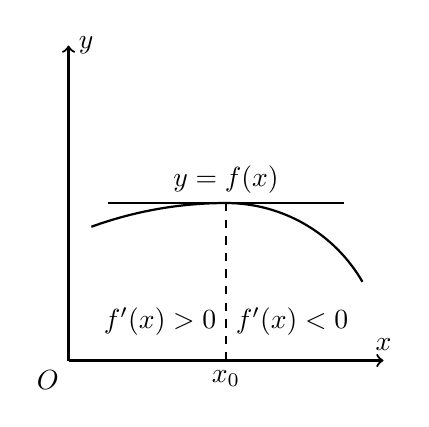
\begin{tikzpicture}
        \draw[thick,->] (0,0) -> (4,0)node[above]{\(x\)};
        \draw[thick,->] (0,0) -> (0,4)node[right]{\(y\)};
        \draw (0,0)node[below left]{\(O\)};
        \draw (2,2)node[above]{\(y=f(x)\)};
        \draw (2,.5)node[left]{\(f'(x)>0\)}node[right]{\(f'(x)<0\)};
        \draw[thick] (2,2)[rotate=90]arc[start angle=0,end angle=-60,radius=2];
        \draw[thick] (2,2)[rotate=90]arc[start angle=0,end angle=20,radius=5];
        \draw (.5,2)--(3.5,2);
        \draw[dashed] (2,2)--(2,0)node[below]{\(x_0\)};
        \end{tikzpicture}
    \subcaption{}
    \end{subfigure}%
    \begin{subfigure}[b]{\subwidth}
    \centering
        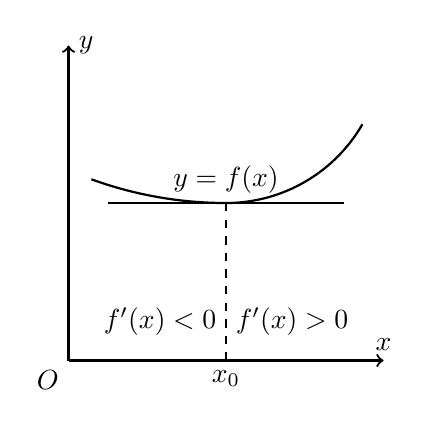
\begin{tikzpicture}
        \draw[thick,->] (0,0) -> (4,0)node[above]{\(x\)};
        \draw[thick,->] (0,0) -> (0,4)node[right]{\(y\)};
        \draw (0,0)node[below left]{\(O\)};
        \draw (2,2)node[above]{\(y=f(x)\)};
        \draw (2,.5)node[left]{\(f'(x)<0\)}node[right]{\(f'(x)>0\)};
        \draw[thick] (2,2)[rotate=-90]arc[start angle=0,end angle=60,radius=2];
        \draw[thick] (2,2)[rotate=-90]arc[start angle=0,end angle=-20,radius=5];
        \draw (.5,2)--(3.5,2);
        \draw[dashed] (2,2)--(2,0)node[below]{\(x_0\)};
        \end{tikzpicture}
    \subcaption{}
    \end{subfigure}%
    \\
    \begin{subfigure}[b]{\subwidth}
    \centering
        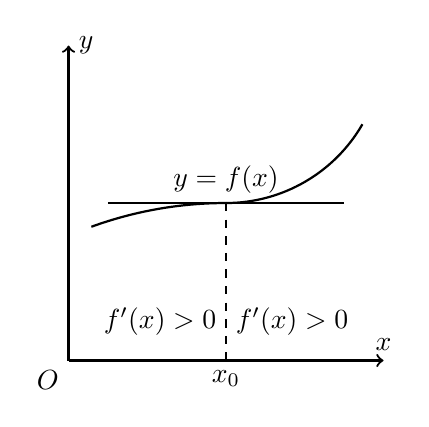
\begin{tikzpicture}
        \draw[thick,->] (0,0) -> (4,0)node[above]{\(x\)};
        \draw[thick,->] (0,0) -> (0,4)node[right]{\(y\)};
        \draw (0,0)node[below left]{\(O\)};
        \draw (2,2)node[above]{\(y=f(x)\)};
        \draw (2,.5)node[left]{\(f'(x)>0\)}node[right]{\(f'(x)>0\)};
        \draw[thick] (2,2)[rotate=-90]arc[start angle=0,end angle=60,radius=2];
        \draw[thick] (2,2)[rotate=90]arc[start angle=0,end angle=20,radius=5];
        \draw (.5,2)--(3.5,2);
        \draw[dashed] (2,2)--(2,0)node[below]{\(x_0\)};
        \end{tikzpicture}
    \subcaption{}
    \end{subfigure}%
    \begin{subfigure}[b]{\subwidth}
    \centering
        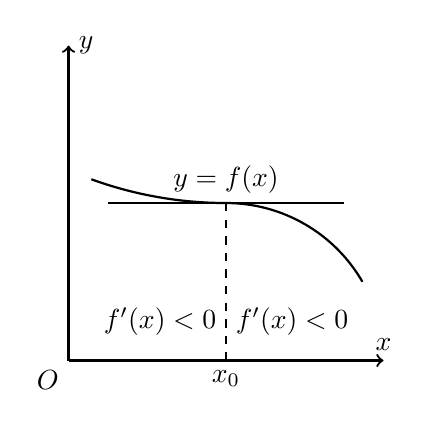
\begin{tikzpicture}
        \draw[thick,->] (0,0) -> (4,0)node[above]{\(x\)};
        \draw[thick,->] (0,0) -> (0,4)node[right]{\(y\)};
        \draw (0,0)node[below left]{\(O\)};
        \draw (2,2)node[above]{\(y=f(x)\)};
        \draw (2,.5)node[left]{\(f'(x)<0\)}node[right]{\(f'(x)<0\)};
        \draw[thick] (2,2)[rotate=90]arc[start angle=0,end angle=-60,radius=2];
        \draw[thick] (2,2)[rotate=-90]arc[start angle=0,end angle=-20,radius=5];
        \draw (.5,2)--(3.5,2);
        \draw[dashed] (2,2)--(2,0)node[below]{\(x_0\)};
        \end{tikzpicture}
    \subcaption{}
    \end{subfigure}%
    \caption{}
\end{figure}

类似地,可证情形2及情形3.
\end{proof}
\end{theorem}
上述定理也可简单地表述为:
当\(x\)在\(x_0\)的邻域内由小及大经过\(x_0\)时,
如果\(f'(x)\)的符号由正变负(即\(f'_-(x_0)>0\)且\(f'_+(x_0)<0\)),
那么\(f(x)\)在\(x_0\)处取得极大值;
如果\(f'(x)\)的符号由负变正(即\(f'_-(x_0)<0\)且\(f'_+(x_0)>0\)),
那么\(f(x)\)在\(x_0\)处取得极小值;
如果\(f'(x)\)的符号并不改变,
那么\(f(x)\)在\(x_0\)处没有极值.

根据\cref{theorem:微分中值定理.函数存在极值的必要条件,theorem:微分中值定理.函数存在极值的第一充分条件},
如果函数\(f(x)\)在所讨论的区间内连续,除个别点歪处处可导,
那么就可以按下列步骤来求\(f(x)\)在该区间内的极值点和相应的极值:
\begin{enumerate}
	\item 求出导数\(f'(x)\);
	\item 求出\(f(x)\)的全部驻点与不可导点;
	\item 考察\(f'(x)\)的符号在每个驻点或不可导点的左右邻域的情形,
	以确定该点是否为极值点;
	如果是极值点,
	进一步确定是极大值点还是极小值点;
	\item 求出各极值点的函数值,就得函数\(f(x)\)的全部极值.
\end{enumerate}

\begin{theorem}[函数存在极值的第二充分条件]\label{theorem:微分中值定理.函数存在极值的第二充分条件}
设函数\(f(x)\)在\(x_0\)处具有二阶导数且\(f'(x_0)=0\),\(f''(x_0)\neq 0\),那么
\begin{enumerate}
	\item 当\(f''(x_0)<0\)时,函数\(f(x)\)在\(x_0\)处取得极大值;
	\item 当\(f''(x_0)>0\)时,函数\(f(x)\)在\(x_0\)处取得极小值.
\end{enumerate}
\end{theorem}
上述定理表明,如果函数\(f(x)\)在驻点\(x_0\)处的二阶导数\(f''(x_0)\neq0\),
那么该驻点\(x_0\)一定是极值点,
并且可以按二阶导数\(f''(x_0)\)的符号来判定\(f(x_0)\)是极大值还是极小值.
但如果\(f''(x_0)=0\),上述定理就不能应用.
事实上,当\(f'(x_0)=0\)且\(f''(x_0)=0\)时,
\(f(x)\)在\(x_0\)处可能有极大值,也可能有极小值,也可能没有极值;
例如,\(f_1(x) = -x^4\),\(f_2(x) = x^4\)和\(f_3(x) = x^3\)
这三个函数在\(x=0\)处就分别属于这三种情况.
因此,如果函数在驻点处的二阶导数为零,
那么还得用一阶导数在驻点左右邻域的符号来判定.

\begin{example}
设函数\(f(x),g(x)\)都具有二阶导数,
且\(g''(x)<0\),\(g(x_0)=a\)是\(g(x)\)的极值,
证明:“\(f'(a)>0\)”是“\(f[g(x)]\)在\(x_0\)取极大值”的充分条件.
\begin{solution}
因为\(g(x_0)=a\)是\(g(x)\)的极值,
所以根据\cref{theorem:微分中值定理.函数存在极值的必要条件}
必有\(g'(x_0)=0\).

记\(F(x) = f[g(x)]\),则\(F'(x) = \eval{f'(u)}_{u=g(x)} \cdot g'(x)\),
\(F''(x) = \eval{f''(u)}_{u=g(x)} \cdot g'(x) \cdot g'(x)
+ \eval{f'(u)}_{u=g(x)} \cdot g''(x)\).
根据\cref{theorem:微分中值定理.函数存在极值的第二充分条件},
要使“\(F(x)=f[g(x)]\)在\(x_0\)取极大值”,只需令\(F''(x_0) < 0\),
那么有\[
	\eval{f'(u_0)}_{u_0=g(x_0)} \cdot g''(x_0) < 0.
\]
由题可知\(g''(x)<0\),
故\(\eval{f'(u_0)}_{u_0=g(x_0)} = f'(a) > 0\),
也就是说“\(f'(a)>0\)”是“\(f[g(x)]\)在\(x_0\)取极大值”的充分条件.
\end{solution}
\end{example}

\subsection{最大值最小值问题}
假定函数\(f(x)\)在闭区间\([a,b]\)上连续,
在开区间\((a,b)\)内除有限个点外可导,
且至多有有限个驻点.
在上述条件下,我们来讨论\(f(x)\)在\([a,b]\)上的最大值和最小值的求法.

首先由闭区间上连续函数的性质,
可知\(f(x)\)在\([a,b]\)上的最大值和最小值一定存在.

其次,如果最大值(或最小值)\(f(x_0)\)在开区间\((a,b)\)内的点\(x_0\)处取得,
那么,按\(f(x)\)在开区间内除有限个点外可导且至多有有限个驻点的假定,
可知\(f(x_0)\)一定也是\(f(x)\)的极大值(或极小值),
从而\(x_0\)一定是\(f(x)\)的驻点或不可导点.
又\(f(x)\)的最大值和最小值也可能在区间的端点处取得.

可用如下的方法求\(f(x)\)在\([a,b]\)上的最大值和最小值:
\begin{enumerate}
	\item 求出\(f(x)\)在\((a,b)\)内的
	驻点\(\AutoTuple{x}{m}\)和不可导点\(x'_1,x'_2,\dotsc,x'_n\);
	\item 计算\(f(x_i)\ (i=1,2,\dotsc,m)\)
	和\(f(x'_j)\ (j=1,2,\dotsc,n)\),
	以及\(f(a)\)和\(f(b)\);
	\item 比较上一步中求出的各个函数值,
	其中最大的就是\(f(x)\)在\([a,b]\)上的最大值,
	最小的就是\(f(x)\)在\([a,b]\)上的最小值.
\end{enumerate}

在求函数的最大值(或最小值)时,特别值得指出的是下述情形:
\(f(x)\)在一个区间(不论有限区间还是无限区间,开区间或闭区间)内可导,
且只有一个驻点\(x_0\),并且这个驻点\(x_0\)是函数\(f(x)\)的极值点,
那么,当\(f(x_0)\)是极大值时,\(f(x_0)\)就是\(f(x)\)在该区间上的最大值;
当\(f(x_0)\)是极小值时,\(f(x_0)\)就是\(f(x)\)在该区间上的最小值.

\section{函数图形的描绘}
借助一阶导数的符号,可以确定函数图形在哪个区间上上升,在哪个区间上下降,在什么地方有极值点;
借助二阶导数的符号,可以确定函数图形在哪个区间上为凹,在哪个区间上为凸,在什么地方有拐点.
知道了函数图形的升降、凹凸以及极值点和拐点后,也就可以掌握函数的性态,并把函数的图形画得比较准确.

现在,随着现代计算机技术的发展,借助计算机和许多数学软件,可以方便地画出各种函数的图形.
但是,如何识别机器作图中的误差,如何掌握图形上的关键点,如何选择作图的范围等,
从而进行人工干预,仍然需要我们有运用微分学的方法描绘图形的基本知识.

利用导数描绘函数图形的一般步骤如下:\begin{enumerate}
	\item 确定函数\(y=f(x)\)的定义域,
	发现函数所具有的某些特性(如有界性、奇偶性、周期性等),
	并求出函数的一阶导数\(f'(x)\)和二阶导数\(f''(x)\);

	\item 求出一阶导数\(f'(x)\)和二阶导数\(f''(x)\)在函数定义域内的全部零点,
	并求出函数\(f(x)\)的间断点及\(f'(x)\)和\(f''(x)\)不存在的点,
	用这些点把函数的定义域划分成几个部分区间;

	\item 确定在这些部分区间内\(f'(x)\)和\(f''(x)\)的符号,
	并由此确定函数图形的升降、凹凸、极值点、拐点;

	\item 确定函数图形的水平渐近线、铅直渐近线、斜渐近线以及其他变化趋势;

	\item 算出\(f'(x)\)和\(f''(x)\)的零点以及不存在的点所对应的函数值,
	定出图形上的相应的点;为了把图形描绘得准确些,有时还需要补充一些点;
	然后结合前两步中得到的结果,联结这些点画出函数\(y=f(x)\)的图形.
\end{enumerate}

\section{曲率}\label{section:微分中值定理.曲率}
\subsection{弧微分}
作为曲率的预备知识,先介绍弧微分的概念.

设函数\(f(x)\)在区间\((a,b)\)内具有连续导数.
在曲线\(y=f(x)\)上取固定点\(M_0(x_0,y_0)\)作为度量弧长的基点,
并规定依\(x\)增大的方向作为曲线的正向.
对曲线上任一点\(M(x,y)\),
规定有向弧段\(\Arc{M_0 M}\)的值\(s\)(简称为弧\(s\))如下:
\(s\)的绝对值等于这弧段的长度,
当有向弧段\(\Arc{M_0 M}\)的方向与曲线的正向一致时\(s>0\),相反时\(s<0\).
显然,弧\(s\)与\(x\)存在函数关系:
\(s = s(x)\),而且\(s(x)\)是\(x\)的单调增加函数.
下面来求\(s(x)\)的导数及微分.

设\(x\)、\(x+\increment x\)为\((a,b)\)内两个邻近的点,
它们在曲线\(y=f(x)\)上的对应点为\(M\)、\(M'\),
并设对应于\(x\)的增量\(\increment x\),
弧\(s\)的增量为\(\increment s\),
那么\[
	\increment s = \Arc{M_0 M'} - \Arc{M_0 M} = \Arc{M M'}.
\]
于是\begin{align*}
	\left(\frac{\increment s}{\increment x}\right)^2
	&= \left(\frac{\Arc{M M'}}{\increment x}\right)^2
	= \left(\frac{\Arc{M M'}}{\abs{M M'}}\right)^2
		\cdot \frac{\abs{M M'}^2}{(\increment x)^2} \\
	&= \left(\frac{\Arc{M M'}}{\abs{M M'}}\right)^2
		\cdot \frac{(\increment x)^2 + (\increment y)^2}{(\increment x)^2} \\
	&= \left(\frac{\Arc{M M'}}{\abs{M M'}}\right)^2
		\cdot \left[ 1 + \left(\frac{\increment y}{\increment x}\right)^2 \right],
\end{align*}\[
\frac{\increment s}{\increment x} = \pm \sqrt{\left(\frac{\Arc{M M'}}{\abs{M M'}}\right)^2 \cdot \left[ 1 + \left(\frac{\increment y}{\increment x}\right)^2 \right]}.
\]
令\(\increment x\to0\)取极限,
由于\(\increment x\to0\)时,
\(M' \to M\),
这时弧的长度与弦的长度之比的极限等于1,
即\[
	\lim_{M' \to M} \frac{\abs{\Arc{M M'}}}{\abs{M M'}} = 1,
\]
又\[
	\lim_{\increment x\to0} \frac{\increment y}{\increment x} = y',
\]
因此得\[
	\dv{s}{x} = \pm \sqrt{1 + (y')^2}.
\]
由于\(s = s(x)\)是单调增加函数,从而上式根号前应取正号,
于是有\begin{equation}
	\dd{s} = \sqrt{1 + (y')^2} \dd{x},
\end{equation}
这就是\DefineConcept{弧微分公式}.

弧微分公式也可写作\begin{equation}
	\dd{s} = \sqrt{(\dd{x})^2 + (\dd{y})^2}.
\end{equation}

\subsection{曲率及其计算公式}
设曲线\(C\)是光滑的(即曲线上每一点处都具有切线,且切线随切点的移动而连续转动),
在曲线\(C\)上选定一点\(M_0\)作为度量弧\(s\)的基点.
设曲线上点\(M\)对应于弧\(s\),
在点\(M\)处切线的倾角为\(\alpha\)
(这里假定曲线\(C\)所在的平面上已设立了\(xOy\)坐标系),
曲线上另外一点\(M'\)对应于弧\(s+\increment s\),
在点\(M'\)处切线的倾角为\(\alpha + \increment \alpha\).
那么,弧段\(\Arc{MM'}\)的长度为\(\abs{\increment s}\).
当动点从\(M\)移动到\(M'\)时切线转过的角度为\(\abs{\increment \alpha}\).

我们用比值\(\frac{\abs{\increment\alpha}}{\abs{\increment s}}\),
即单位弧段上切线转过的角度的大小来表达弧段\(\Arc{MM'}\)的平均弯曲程度,
把这比值叫做弧段\(\Arc{MM'}\)的\DefineConcept{平均曲率},
并记作\(\overline{K}\),即\[
	\overline{K} = \abs{\frac{\increment\alpha}{\increment s}}.
\]

类似于从平均速度引进瞬时速度的方法,
当\(\increment s\to0\)(即\(M' \to M\))时,
上述平均曲率的极限叫做曲线\(C\)在点\(M\)处的\DefineConcept{曲率},
记作\(K\),
即\[
	K \defeq \lim_{\increment s\to0} \abs{\frac{\increment\alpha}{\increment s}}.
\]
在\(\displaystyle \lim_{\increment s\to0} \frac{\increment\alpha}{\increment s}
= \dv{\alpha}{s}\)存在的条件下,
\(K\)也可以表示为\[
	K = \abs{\dv{\alpha}{s}}.
\]

对于直线来说,切线与直线本身重合,
当点沿直线移动时,切线的倾角不变,
\(\increment\alpha = 0\),
\(\frac{\increment\alpha}{\increment s} = 0\),
从而\(K = \abs{\displaystyle\dv{\alpha}{s}} = 0\).
这就是说,直线上任意点\(M\)处的曲率都等于零,这与我们直觉认识到的“直线不弯曲”一致.

\begin{figure}%曲率圆
	\centering
	\begin{tikzpicture}
		\draw[thick,->] (0,0) -> (9,0)node[above]{\(x\)};
		\draw[thick,->] (0,0) -> (0,8)node[right]{\(y\)};
		\pgfmathsetmacro{\cx}{4}
		\pgfmathsetmacro{\cy}{4}
		\pgfmathsetmacro{\cr}{3}
		\coordinate(M)at(\cx,\cy);
		\draw (M)circle(\cr);
		\pgfmathsetmacro{\ta}{30}
		\pgfmathsetmacro{\tb}{80}
		\pgfmathsetmacro{\pax}{\cx+\cr*sin(\ta)}
		\pgfmathsetmacro{\pay}{\cy-\cr*cos(\ta)}
		\pgfmathsetmacro{\pbx}{\cx+\cr*sin(\tb)}
		\pgfmathsetmacro{\pby}{\cy-\cr*cos(\tb)}
		\coordinate(P1)at(\pax,\pay);
		\coordinate(P2)at(\pbx,\pby);
		\draw (M)node[left]{\(D\)}--(P1)node[below]{\(M\)}
			(M)--(P2)node[right]{\(M'\)}node[midway,above]{\(a\)};
		\pgfmathsetmacro{\paz}{\pax+\pay*(\cy-\pay)/(\cx-\pax)}
		\pgfmathsetmacro{\pbz}{\pbx+\pby*(\cy-\pby)/(\cx-\pbx)}
		\coordinate(Q1)at(\paz,0);
		\coordinate(Q2)at(\pbz,0);
		\coordinate(X)at(100,0);
		\draw (Q1)--(P1) (Q2)--(P2);

		\draw pic["\(\increment\alpha\)",draw=orange,-,below right]{angle=P1--M--P2};
		\draw pic["\(\alpha\)",draw=orange,-,angle eccentricity=1.5,angle radius=5mm]{angle=X--Q1--P1};
		\draw pic["\(\alpha+\increment\alpha\)",draw=orange,-,angle eccentricity=1,angle radius=3mm,above right]{angle=X--Q2--P2};
		\draw pic[draw=gray,-,angle radius=0.3cm]{right angle=M--P1--Q1};
		\draw pic[draw=gray,-,angle radius=0.3cm]{right angle=M--P2--Q2};
	\end{tikzpicture}
	\caption{曲率圆}
	\label{figure:微分中值定理.曲率圆}
\end{figure}

设圆的半径为\(a\),由\cref{figure:微分中值定理.曲率圆} 可见,
圆在点\(M\)、\(M'\)处的切线所夹的角\(\increment\alpha\)等于中心角,
即\[
	\angle{M D M'} = \increment\alpha.
\]
但是\[
	\angle{M D M'} = \frac{\increment s}{a},
\]
于是\[
	\frac{\increment\alpha}{\increment s}
	= \frac{\increment s / a}{\increment s}
	= \frac{1}{a},
\]
从而\[
	K = \abs{\dv{\alpha}{s}} = \frac{1}{a}.
\]
因为点\(M\)是圆上任意取定的一点,
上述结论表示,
圆上各点处的曲率都等于半径\(a\)的倒数\(\frac{1}{a}\),
这就是说,圆的弯曲程度到处一样;
且半径越小的圆,曲率越大,即圆弯曲得越厉害.

设曲线的直角坐标方程为\(y=f(x)\),
且\(f(x)\)具有二阶导数(这时\(f'(x)\)连续,从而曲线是光滑的).
因为\(\tan\alpha = y'\),
所以再在等号两边同时对\(x\)求导便得\[
	\sec^2\alpha \dv{\alpha}{x} = y'',
\]
即\[
	\dv{\alpha}{x}
	= \frac{y''}{\sec^2\alpha}
	= \frac{y''}{1 + \tan^2\alpha}
	= \frac{y''}{1 + (y')^2},
\]
于是\[
	\dd{\alpha}
	= \frac{y''}{1 + (y')^2} \dd{x}.
\]
又因为\(\dd{s} = \sqrt{1+(y')^2} \dd{x}\),
从而有\begin{equation}
	K
	= \abs{\dv{\alpha}{s}}
	= \frac{1}{\sqrt{1+(y')^2}}
	\abs{\frac{y''}{1 + (y')^2}}
	= \frac{\abs{y''}}{(1+(y')^2)^{\frac32}}.
\end{equation}

设曲线由参数方程\(\left\{ \begin{array}{c}
	x = \phi(t) \\
	y = \psi(t)
\end{array} \right.\)给出,
由\cref{equation:导数.参数方程确定的函数的一阶导数,equation:导数.参数方程确定的函数的二阶导数}
可知\[
	y' = \frac{\psi'(t)}{\phi'(t)}, \qquad
	y'' = \frac{\psi''(t) \phi'(t) - \psi'(t) \phi''(t)}{(\phi'(t))^3},
\]
那么有\begin{equation}
	K = \frac{
		\abs{\phi'(t)\psi''(t)-\phi''(t)\psi'(t)}
	}{
		[(\phi'(t))^2+(\psi'(t))^2]^{\frac32}
	}.
\end{equation}

在某些实际问题中,
\(\abs{y'}\)同\(1\)比较起来是很小的(即\(\abs{y'} \ll 1\)),可以忽略不计,
这时,由\(1 + (y')^2 \approx 1\),而有曲率的近似计算公式为\[
	K \approx \abs{y''}.
\]
这就是说,当\(\abs{y'} \ll 1\)时,
曲率\(K\)近似于\(\abs{y''}\).
经过这样的简化之后,对一些复杂问题的计算和讨论就方便多了.

\subsection{曲率圆与曲率半径}
设曲线\(y=f(x)\)在点\(M(x,y)\)处的曲率为\(K\ (K\neq0)\).
在点\(M\)处的曲线的发现上,在凹的一侧取一点\(D\),使\(\abs{DM} = \frac{1}{K} = \rho\).
以\(D\)为圆心,\(\rho\)为半径作圆,这个圆叫做曲线在点\(M\)处的\DefineConcept{曲率圆},
曲率圆的圆心\(D\)叫做曲线在点\(M\)处的\DefineConcept{曲率中心},
曲率圆的半径\(\rho\)叫做曲线在点\(M\)处的\DefineConcept{曲率半径}.

按上述规定可知,曲率圆与曲线在点\(M\)有相同的切线和曲率,且在点\(M\)邻近有相同的凹向.
因此,在实际问题中,常常用曲率圆在点\(M\)邻近的一段圆弧来近似代替曲线弧,以使问题简化.

按上述规定,曲线在点\(M\)处的曲率\(K\ (K\neq0)\)
与曲线在点\(M\)处的曲率半径\(\rho\)有如下的关系:\[
	\rho = \frac{1}{K}, \qquad
	K = \frac{1}{\rho}.
\]
这就是说:曲线上一点处的曲率半径与曲线在该点处的曲率互为倒数.

\begin{example}
求出对数曲线\(y = \ln x\)上曲率半径最小的点.
\begin{solution}
显然有\(y' = \frac{1}{x}\),\(y'' = -\frac{1}{x^2}\),那么曲率为\[
	K = \frac{\abs{y''}}{(1+(y')^2)^{\frac32}}
	= \frac{1/x^2}{(1+1/x^2)^{\frac32}}
	= \frac{x}{(1+x^2)^{\frac32}}.
\]
曲率\(K\)对\(x\)求导得\[
	K' = \frac{(1+x^2)^{\frac32} - x \frac32 (1+x^2)^{\frac12} 2x}{(1+x^2)^3}
	= \frac{1 - 2x^2}{(1+x^2)^{\frac52}}.
\]
令\(K' = 0\),考虑\(x>0\),
解得\(x_0 = \frac{1}{\sqrt{2}}\).
当\(0<x<x_0\)时,\(K'>0\);
当\(x>x_0\)时,\(K'<0\);
说明\(K'\)在\(x=x_0\)时取得极大值.
而曲率半径最小的点就是曲率最大的点,
即\(x = \frac{1}{\sqrt{2}}\)时,
曲率半径最小值为\(\frac{3\sqrt{3}}{2}\).
\end{solution}
\end{example}

\subsection{曲率中心的计算公式以及渐屈线、渐伸线}
设已知曲线的方程是\(y=f(x)\),
且其二阶导数\(y''\)在点\(x\)不为零.
又设曲线\(y=f(x)\)在点\(M(x,y)\)的曲率为\(K\),
曲率中心为\(D(\alpha,\beta)\),
曲率半径为\(\rho=K^{-1}\),
那么曲率圆的方程为\[
	(\xi-\alpha)^2+(\eta-\beta)^2=\rho^2,
	\quad(\xi,\eta)\in\mathbb{R}^2.
\]

因为\(M(x,y)\)在这个曲率圆上,所以满足曲率圆的方程,
有\begin{equation}\label{equation:曲率圆.曲率中心的推导1}
	(x-\alpha)^2+(y-\beta)^2=\rho^2.
\end{equation}
又因为曲线在点\(M\)的切线与曲率圆的半径\(DM\)垂直,
两者的斜率分别为\[
	y'
	\quad\text{和}\quad
	\frac{y-\beta}{x-\alpha},
\]
所以\[
	y' \cdot \frac{y-\beta}{x-\alpha} = -1,
\]
即\begin{equation}\label{equation:曲率圆.曲率中心的推导2}
	y' = -\frac{x-\alpha}{y-\beta}.
\end{equation}
由\cref{equation:曲率圆.曲率中心的推导1,equation:曲率圆.曲率中心的推导2}
消去\(x-\alpha\),解出\[
	(y-\beta)^2
	=\frac{\rho^2}{1+(y')^2}
	=\frac{(1+(y')^2)^2}{(y'')^2}.
\]

由于当\(y''>0\)时,曲线\(y=f(x)\)是凹弧,\(y-\beta<0\);
当\(y''<0\)时,曲线是凸弧,\(y-\beta>0\).
总之,\(y''\)与\(y-\beta\)异号.
因此取上式两边的平方根,得\[
	y-\beta
	=-\frac{1+(y')^2}{y''};
\]
于是\[
	x-\alpha
	=-y'(y-\beta)
	=\frac{y'(1+(y')^2)}{y''}.
\]

因此,曲线在对应点\(M(x,y)\)的曲率中心\(D(\alpha,\beta)\)的坐标为
\begin{equation}
	\left\{ \def\arraystretch{1.5} \begin{array}{l}
		\alpha = x - y' \frac{1 + (y')^2}{y''}, \\
		\beta = y + \frac{1 + (y')^2}{y''}.
	\end{array} \right.
\end{equation}

当点\((x,f(x))\)沿曲线\(C\)移动时,
相应的曲率中心\(D\)的轨迹曲线\(G\)称为曲线\(C\)的\DefineConcept{渐屈线},
相对地,曲线\(C\)称为曲线\(G\)的\DefineConcept{渐伸线}.
%微分中值定理
\chapter{不定积分}\label{chapter:不定积分}
\section{不定积分的概念与性质}
在\cref{chapter:导数}我们已经介绍了求导运算.
现在我们来探索求导运算的逆运算.

\subsection{原函数与不定积分的概念}
\begin{definition}
如果在区间\(I\)上,可导函数\(F(x)\)的导函数为\(f(x)\),
即对任一\(x \in I\),都有\[
	F'(x)=f(x) \quad\text{或}\quad \dd{F(x)}=f(x) \dd{x},
\]
那么函数\(F(x)\)就称为
“\(f(x)\)(或\(f(x) \dd{x}\))在区间\(I\)上的\DefineConcept{原函数}”.
\end{definition}

关于原函数,我们首先要问:
一个函数具备什么条件,才能保证它的原函数一定存在?
这个问题将在下一章中讨论,这里先介绍一个结论.
\begin{theorem}[原函数存在定理]%提前叙述该定理.参见\cref{theorem:定积分.原函数存在定理}
如果函数\(f(x)\)在区间\(I\)上连续,
那么在区间\(I\)上存在可导函数\(F(x)\),使对任一\(x \in I\)都有\[
	F'(x)=f(x).
\]
换言之,连续函数一定有原函数.
\end{theorem}
下面还要说明两点.

第一,如果\(f(x)\)在区间\(I\)上有原函数,
即有一个函数\(F(x)\),
使对任一\(x \in I\),
都有\(F'(x) = f(x)\),
那么,对任何常数\(C\),显然也有\[
	[F(x) + C]' = f(x),
\]即对任何常数\(C\),函数\(F(x) + C\)也是\(f(x)\)的原函数.
这说明,如果\(f(x)\)有一个原函数,那么\(f(x)\)就有无限多个原函数.

第二,如果在区间\(I\)上\(F(x)\)是\(f(x)\)的一个原函数,
那么\(f(x)\)的其他原函数与\(F(x)\)有什么关系?

设\(\Phi(x)\)是\(f(x)\)的另一个原函数,
即对任一\(x \in I\)有\[
	\Phi'(x) = f(x),
\]
于是\[
	[\Phi(x) - F(x)]' = \Phi'(x) - F'(x) = f(x) - f(x) = 0.
\]
在前面章节已经知道,
在一个区间上导数恒为零的函数必为常数,所以\[
	\Phi(x) - F(x) = C_0,
\]
其中\(C_0\)是某个常数.这就表明\(\Phi(x)\)与\(F(x)\)只差一个常数.
因此,当\(C\)为任意的常数时,
表达式\(F(x) + C\)就可表示\(f(x)\)的任意一个原函数.
也就是说,\(f(x)\)的全体原函数所组成的集合,就是函数族\[
	\Set{ F(x) + C \given C \in (-\infty,\infty) }.
\]

\begin{definition}
在区间\(I\)上,
函数\(f(x)\)的带有任意常数项的原函数
称为\(f(x)\)(或\(f(x) \dd{x}\))在区间\(I\)上的\DefineConcept{不定积分},
记作\[
	\int f(x) \dd{x},
\]
其中记号\(\int\)称为\DefineConcept{积分号},
\(f(x)\)称为\DefineConcept{被积函数},
\(f(x)\dd{x}\)称为\DefineConcept{被积表达式},
\(x\)称为\DefineConcept{积分变量}.
\end{definition}
由此定义及前面的说明可知,
如果\(F(x)\)是\(f(x)\)在区间\(I\)上的一个原函数,
那么\(F(x) + C\)就是\(f(x)\)的不定积分,
即\[
	\int f(x) \dd{x} = F(x) + C.
\]
因而不定积分\(\int f(x) \dd{x}\)可以表示\(f(x)\)的任意一个原函数.

对初等函数来说,在其定义区间上,它的原函数一定存在,但原函数不一定都是初等函数,如\[
	\int e^{-x^2} \dd{x}, \qquad
	\int \frac{\sin x}{x} \dd{x}, \qquad
	\int \frac{\dd{x}}{\ln{x}}, \qquad
	\int \frac{\dd{x}}{\sqrt{1+x^4}}
\]
等等,它们的原函数就都不是初等函数.

\begin{example}
求\(\int \frac{\dd{x}}{x}\).
\begin{solution}
当\(x > 0\)时,由于\((\ln x)' = \frac{1}{x}\),
所以\(\ln x\)是\(\frac{1}{x}\)在区间\((0,+\infty)\)内的一个原函数.
因此,在\((0,+\infty)\)内,\[
\int \frac{\dd{x}}{x} = \ln x + C_1.
\]

当\(x < 0\)时,
由于\([\ln(-x)]' = \frac{1}{-x} \cdot (-1) = \frac{1}{x}\),
所以\(\ln(-x)\)是\(\frac{1}{x}\)在\((-\infty,0)\)内的一个原函数.
因此,在\((-\infty,0)\)内,\[
	\int \frac{\dd{x}}{x} = \ln(-x) + C_2.
\]

把在\(x > 0\)及\(x < 0\)内的结果合起来,
可写作\begin{equation}
	\int \frac{\dd{x}}{x} = \left\{ \begin{array}{lc}
		\ln x + C_1, & x>0, \\
		\ln(-x) + C_2, & x<0.
	\end{array} \right.
\end{equation}
虽然常数\(C_1\)和\(C_2\)的取值可以是独立的,
但在不严谨的情况下,为方便记忆,上式也可写作\begin{equation}
	\int \frac{\dd{x}}{x} = \ln\abs{x} + C.
\end{equation}
\end{solution}
\end{example}

\begin{definition}
函数\(f(x)\)的原函数的图形称为\(f(x)\)的积分曲线.
\end{definition}

从不定积分的定义,即可知以下关系:
\begin{align*}
	\text{\(\int f(x) \dd{x}\)是\(f(x)\)的原函数}
	&\iff
	\dv{x}\relax\left[ \int f(x) \dd{x} \right] = f(x) \\
	&\iff
	\dd\relax\left[\int f(x) \dd{x}\right] = f(x) \dd{x}. \\
	\text{\(F(x)\)是\(F'(x)\)的原函数}
	&\iff
	\int F'(x) \dd{x} = F(x) + C \\
	&\iff
	\int \dd{F(x)} = F(x) + C.
\end{align*}

由此可见,微分运算(以记号\(\dd\relax\)表示)
与求不定积分的运算(简称积分运算,以记号\(\int\)表示)是互逆的;
当记号\(\int\)与\(\dd\relax\)连在一起时,或者抵消,或者抵消后差一个常数.

\subsection{不定积分的性质}
\begin{property}\label{theorem:不定积分.性质1}
设函数\(f(x)\)及\(g(x)\)的原函数存在,则\[
	\int \bigl[f(x) + g(x)\bigr] \dd{x}
	= \int f(x) \dd{x}
	+ \int g(x) \dd{x}.
\]
\end{property}
这个性质对于有限个函数都是成立的.

\begin{example}
求\(\int \tan^2 x \dd{x}\).
\begin{solution}
根据三角恒等式\(\tan^2 x + 1 = \sec^2 x\),有\[
	\int \tan^2 x \dd{x}
	= \int (\sec^2 x - 1) \dd{x}
	= \int \sec^2 x \dd{x} - \int \dd{x}
	= \tan x - x + C.
\]
\end{solution}
\end{example}

\begin{property}\label{theorem:不定积分.性质2}
设函数\(f(x)\)的原函数存在,\(k\)为非零常数,则\[
	\int k f(x) \dd{x} = k \int f(x) \dd{x}.
\]
\end{property}
\begin{remark}
我们在\cref{theorem:不定积分.性质2} 中强调\(k\neq0\),
是因为如果\(k=0\),那么上式右边为\(0 \int f(x) \dd{x} = 0\),
而上式左边\(\int 0 f(x) \dd{x}\)却是全体常数函数的集合,
这就造成了定义上的混乱.
\end{remark}

\section{换元积分法}
利用基本积分表与积分的性质,我们可以计算的不定积分是非常有限的.
因此,有必要进一步来研究不定积分的求法.
本节把复合函数的微分法反过来用于求解不定积分,
利用中间变量的代换,得到复合函数的积分法,
称为\DefineConcept{换元积分法},简称\DefineConcept{换元法}.

\subsection{第一类换元法}
\begin{theorem}
设\(f(u)\)具有原函数,\(u=\phi(x)\)可导,则有换元公式\[
	\int f\bigl[\phi(x)\bigr] \phi'(x) \dd{x}
	= \left[ \int f(u) \dd{u} \right]_{u=\phi(x)}.
\]
\begin{proof}
设\(f(u)\)的原函数是\(F(u)\),即\[
	F'(u) = f(u),
	\qquad
	\int f(u) \dd{u} = F(u) + C.
\]
因为\(u = \phi(x)\)可导,
那么,根据复合函数微分法,
有\[
	\dd{F\left[\phi(x)\right]} = f\left[\phi(x)\right] \phi'(x) \dd{x},
\]
从而根据不定积分的定义有\[
	\int f\bigl[\phi(x)\bigr] \phi'(x) \dd{x}
	= F\bigl[\phi(x)\bigr] + C
	= \left[ \int f(u) \dd{u} \right]_{u=\phi(x)}.
	\qedhere
\]
\end{proof}
\end{theorem}

\begin{example}
求\(\int \frac{\dd{x}}{3+2x}\).
\begin{solution}
令\(u = 3+2x\),
那么被积函数\(\frac{1}{3+2x} = \frac{1}{u}\).
这里缺少\(\displaystyle\dv{u}{x}=2\)这样一个因子,
但由于\(\displaystyle\dv{u}{x}\)是个常数,
故可改变系数凑出这个因子:\[
	\frac{1}{3+2x}
	= \frac{1}{2} \cdot \frac{1}{3+2x} \cdot 2
	= \frac{1}{2} \cdot \frac{1}{3+2x} (3+2x)',
\]
从而\begin{align*}
	\int \frac{\dd{x}}{3+2x}
	&= \frac{1}{2} \int \frac{1}{3+2x} (3+2x)' \dd{x}
	= \frac{1}{2} \int \frac{\dd{u}}{u} \\
	&= \frac{1}{2} \ln\abs{u} + C
	= \frac{1}{2} \ln\abs{3+2x} + C.
\end{align*}
\end{solution}
\end{example}

\begin{remark}
%@see: 《高等数学(第六版 上册)》 P195
一般地,对于积分\(\int f(ax+b) \dd{x}\),
总可作变换\(u=ax+b\),
把它化为\begin{align*}
	\int f(ax+b) \dd{x}
	&= \int \frac{1}{a} f(ax+b) \dd(ax+b) \\
	&= \frac{1}{a} \left[ \int f(u) \dd{u} \right]_{u=ax+b}.
\end{align*}
\end{remark}

\begin{example}
求\(\int 2x e^{x^2} \dd{x}\).
\begin{solution}
令\(u=x^2\),
则被积函数\(2x e^{x^2} = e^{x^2} (x^2)' = e^u u'\),
于是\[
	\int 2x e^{x^2} \dd{x}
	= \int e^u \dd{u}
	= e^u + C
	= e^{x^2} + C.
\]
\end{solution}
\end{example}

\begin{example}
求\(\int x \sqrt{1-x^2} \dd{x}\).
\begin{solution}
令\(u=1-x^2\),
则\(\dd{u} = -2x\dd{x}\),
\(-\frac{1}{2}\dd{u} = x\dd{x}\),
因此\begin{align*}
	\int x \sqrt{1-x^2} \dd{x}
	&= \int u^{\frac{1}{2}} \left(-\frac{1}{2}\right) \dd{u}
	= -\frac{1}{2} \frac{u^{\frac{3}{2}}}{\frac{3}{2}} + C \\
	&= -\frac{1}{3} u^{\frac{3}{2}} + C
	= -\frac{1}{3} (1-x^2)^{\frac{3}{2}} + C.
\end{align*}
\end{solution}
\end{example}

\begin{example}
求\(\int \frac{\dd{x}}{a^2+x^2}\).
\begin{solution}
令\(u=\frac{x}{a}\),
\(\dd{x}=a\dd{u}\),
\(\frac{1}{a^2+x^2}
= \frac{1}{a^2(1+u^2)}\),
于是\begin{align}
	\int \frac{\dd{x}}{a^2+x^2}
	&= \int \frac{1}{a^2(1+u^2)} \cdot a\dd{u}
		\nonumber \\
	&= \frac{1}{a} \int \frac{\dd{u}}{1+u^2}
		\nonumber \\
	&= \frac{1}{a} \arctan u + C
		\nonumber \\
	&= \frac{1}{a} \arctan\frac{x}{a} + C.
\end{align}
\end{solution}
\end{example}

\begin{example}
求\(\int \frac{\dd{x}}{\sqrt{a^2-x^2}}\ (a>0)\).
\begin{solution}
令\(u=\frac{x}{a}\),
\(\dd{x}=a\dd{u}\),
\(\frac{1}{\sqrt{a^2-x^2}}
= \frac{1}{a\sqrt{1-u^2}}\),
于是\begin{align}
	\int \frac{\dd{x}}{\sqrt{a^2-x^2}}
	&= \int \frac{1}{a\sqrt{1-u^2}} \cdot a\dd{u}
		\nonumber \\
	&= \int \frac{\dd{u}}{\sqrt{1-u^2}}
		\nonumber \\
	&= \arcsin u + C
		\nonumber \\
	&= \arcsin\frac{x}{a} + C.
\end{align}
\end{solution}
\end{example}

\begin{example}
求\(\int \frac{\dd{x}}{x^2 - a^2}\).
\begin{solution}
因为\[
	\frac{1}{x^2 - a^2}
	= \frac{1}{2a} \left(\frac{1}{x-a} - \frac{1}{x+a}\right),
\]
所以\begin{align}
	\int \frac{\dd{x}}{x^2 - a^2}
	&= \frac{1}{2a} \int \left(\frac{1}{x-a} - \frac{1}{x+a}\right) \dd{x}
		\nonumber \\
	&= \frac{1}{2a} \left[ \int \frac{\dd(x-a)}{x-a} - \int \frac{\dd(x+a)}{x+a} \right]
		\nonumber \\
	&= \frac{1}{2a} ( \ln\abs{x-a} - \ln\abs{x+a} ) + C
		\nonumber \\
	&= \frac{1}{2a} \ln\abs{\frac{x-a}{x+a}} + C.
\end{align}
\end{solution}
\end{example}

\begin{example}
求\(\int \sin mx \cos nx \dd{x}\ (m \neq n)\).
\begin{solution}
由\cref{equation:函数.三角函数.和积互化公式7},
\[
	\sin mx \cos nx
	= \frac12 [\sin(m+n)x + \sin(m-n)x],
\]
于是\begin{align}
	\int \sin mx \cos nx \dd{x}
	&= \frac12 \left[
		\int \sin(m+n)x \dd{x}
		+ \int \sin(m-n)x \dd{x}
	\right]
	\nonumber \\
	&= -\frac{\cos(m+n)x}{2(m+n)}
		- \frac{\cos(m-n)x}{2(m-n)}
		+ C.
\end{align}
\end{solution}
\end{example}

\begin{example}
求\(\int \sin mx \sin nx \dd{x}\ (m \neq n)\).
\begin{solution}
由\cref{equation:函数.三角函数.和积互化公式10},
\[
	\sin mx \sin nx
	= -\frac12 [\cos(m+n)x - \cos(m-n)x],
\]
于是\begin{align}
	\int \sin mx \sin nx \dd{x}
	&= -\frac12 \left[
		\int \cos(m+n)x \dd{x}
		- \int \cos(m-n)x \dd{x}
	\right]
	\nonumber \\
	&= \frac{\sin(m-n)x}{2(m-n)}
		- \frac{\sin(m+n)x}{2(m+n)}
		+ C.
\end{align}
\end{solution}
\end{example}

\begin{example}
求\(\int \cos mx \cos nx \dd{x}\ (m \neq n)\).
\begin{solution}
由\cref{equation:函数.三角函数.和积互化公式9},
\[
	\cos mx \cos nx
	= \frac12 [\cos(m+n)x + \cos(m-n)x],
\]
于是\begin{align}
	\int \cos mx \cos nx \dd{x}
	&= \frac12 \left[
		\int \cos(m+n)x \dd{x}
		+ \int \cos(m-n)x \dd{x}
	\right]
	\nonumber \\
	&= \frac{\sin(m+n)x}{2(m+n)}
		+ \frac{\sin(m-n)x}{2(m-n)}
		+ C.
\end{align}
\end{solution}
\end{example}

\begin{example}
求\(\int \sin^3 x \dd{x}\).
\begin{solution}
\(\begin{aligned}[t]
	\int \sin^3 x \dd{x}
	&= \int \sin^2 x \cdot \sin x \dd{x}
	= -\int (1 - \cos^2 x) \dd(\cos x) \\
	&= -\cos x + \frac{1}{3} \cos^3 x + C.
\end{aligned}\)
\end{solution}
\end{example}

\begin{remark}
%@see: 《高等数学(第六版 上册)》 P197
一般地,对于\(\sin^{2k+1} x \cos^n x\)或\(\sin^n x \cos^{2k+1} x\)
(其中\(k\in\mathbb{N}\))型函数的积分,
总可依次作变换\(u = \cos x\)或\(u = \sin x\),求得结果.
\end{remark}

\begin{example}
%@see: 《高等数学(第六版 上册)》 P197 例13
求\(\int \tan x \dd{x}\).
\begin{solution}
由\cref{equation:三角函数.正切与正余弦的关系}
有\(\tan x = \frac{\sin x}{\cos x}\),
所以\begin{align*}
	\int \tan x \dd{x}
	&= \int \frac{\sin x}{\cos x} \dd{x}
	= - \int \frac{1}{\cos x} \dd(\cos x) \\
	&= - \ln\abs{\cos x} + C.
\end{align*}
\end{solution}
\end{example}

%@see: 《高等数学(第六版 上册)》 P198
类似地可得\(\int \cot x \dd{x} = \ln\abs{\sin x} + C\).

\begin{example}
%@see: 《高等数学(第六版 上册)》 P198 例14
求\(\int \cos^2 x \dd{x}\).
\begin{solution}
\(\begin{aligned}[t]
	\int \cos^2 x \dd{x}
	&= \int \frac{1 + \cos 2x}{2} \dd{x}
	= \frac{1}{2} \left( \int \dd{x} + \int \cos 2x \dd{x} \right) \\
	&= \frac{1}{2} \int \dd{x} + \frac{1}{4} \int \cos 2x \dd(2x) \\
	&= \frac{x}{2} + \frac{\sin 2x}{4} + C.
\end{aligned}\)
\end{solution}
\end{example}

\begin{example}
%@see: 《高等数学(第六版 上册)》 P198 例15
求\(\int \sin^2 x \cos^4 x \dd{x}\).
\begin{solution}
\(\begin{aligned}[t]
	\int \sin^2 x \cos^4 x \dd{x}
	&= \frac{1}{8} \int (1 - \cos 2x) (1 + \cos 2x)^2 \dd{x} \\
	&= \frac{1}{8} \int (1 + \cos 2x - \cos^2 2x - \cos^3 2x) \dd{x} \\
	&= \frac{1}{8} \int (\cos 2x - \cos^3 2x) \dd{x}
		+ \frac{1}{8} \int (1 - \cos^2 2x) \dd{x} \\
	&= \frac{1}{8} \int \sin^2 2x \frac{1}{2} \dd(\sin 2x)
		+ \frac{1}{8} \int \frac{1}{2} (1 - \cos 4x) \dd{x} \\
	&= \frac{1}{48} \sin^3 2x + \frac{1}{16} x - \frac{1}{64} \sin 4x + C.
\end{aligned}\)
\end{solution}
\end{example}

\begin{remark}
%@see: 《高等数学(第六版 上册)》 P198
一般地,对于\(\sin^{2k} x \cos^{2l} x\ (k,l\in\mathbb{N})\)型函数,
总可利用三角恒等式\[
	\sin^2 x = \frac{1}{2} (1 - \cos 2x)
	\quad\text{和}\quad
	\cos^2 x = \frac{1}{2} (1 + \cos 2x)
\]把积分函数化为\(\cos 2x\)的多项式.
\end{remark}

\begin{example}
%@see: 《高等数学(第六版 上册)》 P198 例16
求\(\int \sec^6x \dd{x}\).
\begin{solution}
\(\begin{aligned}[t]
	\int \sec^6x \dd{x}
	&= \int (\sec^2x)^2 \sec^2x \dd{x} \\
	&= \int (1+\tan^2x)^2 \dd(\tan x) \\
	&= \int (1+2\tan^2x+\tan^4x) \dd(\tan x) \\
	&= \tan x + \frac23 \tan^3x + \frac15 \tan^5x + C.
\end{aligned}\)
\end{solution}
\end{example}

\begin{remark}
一般的,对于\(\tan^n x \sec^{2k} x\)
或\(\tan^{2k+1} x \sec^n x\ (k \in \mathbb{N}^+)\)型函数的积分,
可依次作变换\(u=\tan x\)或\(u=\sec x\),
利用三角恒等式\(\sec^2 x = \tan^2 x + 1\)
和微分公式\(\dd(\tan x) = \sec^2 x \dd{x}\),
\(\dd(\sec x) = \sec x \tan x \dd{x}\),
求得结果.
\end{remark}

\begin{example}
%@see: 《高等数学(第六版 上册)》 P199 例18
求\(\int \csc x \dd{x}\).
\begin{solution}
直接计算得
\begin{align*}
	\int \csc x \dd{x}
	&= \int \frac{\dd{x}}{\sin x}
	= \int \frac{\dd{x}}{2 \sin\frac{x}{2} \cos\frac{x}{2}} \\
	&= \int \frac{\dd(\frac{x}{2})}{\tan\frac{x}{2} \cos^2\frac{x}{2}}
	= \int \frac{\dd(\tan\frac{x}{2})}{\tan\frac{x}{2}} \\
	&= \ln\abs{\tan\frac{x}{2}} + C.
\end{align*}
\end{solution}
\end{example}

\begin{example}
%@see: 《高等数学(第六版 上册)》 P199 例19
求\(\int \sec x \dd{x}\).
\begin{solution}
直接计算得\begin{align*}
	\int \sec x \dd{x}
	&= \int \csc\left(x+\frac\pi2\right) \dd(x+\frac\pi2) \\
	&= \ln\abs{\csc\left(x+\frac\pi2\right)-\cot\left(x+\frac\pi2\right)} + C \\
	&= \ln\abs{\sec x+\tan x} + C.
\end{align*}
\end{solution}
\end{example}
\begin{remark}
不定积分\(\int \sec x \dd{x}\)还有其他计算方式:
\begin{enumerate}
	\item \(\begin{aligned}[t]
		\int \sec x \dd{x}
		= \int \frac{\sec x (\sec x + \tan x)}{\sec x + \tan x} \dd{x}
		= \int \frac{\dd(\sec x + \tan x)}{\sec x + \tan x}
		= \ln\abs{\sec x + \tan x} + C.
	\end{aligned}\)

	\item \(\begin{aligned}[t]
		\int \sec x \dd{x}
		= \int \frac{\dd{x}}{\cos x}
		= \int \frac{\cos x \dd{x}}{\cos^2x}
		= \int \frac{\dd(\sin x)}{1 - \sin^2x}
		= \frac12 \ln\abs{\frac{1+\sin x}{1-\sin x}} + C.
	\end{aligned}\)
\end{enumerate}
\end{remark}

\subsection{第二类换元法}
\begin{theorem}
%@see: 《高等数学(第六版 上册)》 P201 定理2
设\(x = \psi(t)\)是单调的、可导的函数,
并且\(\psi'(t) \neq 0\).又设\(f[\psi(t)] \psi'(t)\)具有原函数,
则有换元公式\[
	\int f(x) \dd{x}
	= \left[ \int f[\psi(t)] \psi'(t) \dd{t} \right]_{t=\psi^{-1}(x)},
\]
其中\(t=\psi^{-1}(x)\)是\(x=\psi(t)\)的反函数.
\begin{proof}
设\(f[\psi(t)] \psi'(t)\)的原函数为\(\Phi(t)\),
记\(\Phi[\psi^{-1}(x)] = F(x)\),
利用复合函数及反函数的求导法则,
得到\[
	F'(x) = \dv{\Phi}{t} \cdot \dv{t}{x}
	= f[\psi(t)] \psi'(t) \cdot \frac{1}{\psi'(t)}
	= f[\psi(t)] = f(x),
\]
即\(F(x)\)是\(f(x)\)的原函数,
所以有\begin{align*}
	\int f(x) \dd{x} &= F(x) + C
	= \Phi[\psi^{-1}(x)] + C \\
	&= \left[ \int f[\psi(t)] \psi'(t) \dd{t} \right]_{t=\psi^{-1}(x)}.
	\qedhere
\end{align*}
\end{proof}
\end{theorem}

\begin{example}
%@see: 《高等数学(第六版 上册)》 P201 例21
求\(\int \sqrt{a^2 - x^2} \dd{x}\).
\begin{solution}
求这个积分的困难在于根式\(\sqrt{a^2-x^2}\),
但我们可以利用三角恒等式\(\sin^2t+\cos^2t=1\)来化去根式.
设\(x = a \sin t\ (-\frac{\pi}{2} < x < \frac{\pi}{2})\),
那么\(t = \arcsin\frac{x}{a}\),
\(\sqrt{a^2 - x^2} = \sqrt{a^2 - a^2 \sin^2 t} = a \cos t\),
\(\dd{x} = a \cos t \dd{t}\),
于是根式化成了三角式,
所求积分化为\begin{align*}
	\int \sqrt{a^2 - x^2} \dd{x}
	&= \int a \cos t \cdot a \cos t \dd{t}
	= a^2 \int \cos^2 t \dd{t} \\
	&= a^2 \left( \frac{t}{2} + \frac{\sin 2t}{4} \right) + C \\
	&= \frac{1}{2} a^2 t + \frac{1}{2} a^2 \sin t \cos t + C.
\end{align*}
于是所求积分为\[
	\int \sqrt{a^2 - x^2} \dd{x}
	= \frac{1}{2} a^2 \arcsin\frac{x}{a} + \frac{1}{2} x \sqrt{a^2 - x^2} + C.
\]
\end{solution}
\end{example}

\begin{example}
%@see: 《高等数学(第六版 上册)》 P202 例22
求\(\int \frac{\dd{x}}{\sqrt{x^2 + a^2}}\ (a>0)\).
\begin{solution}
和上例类似,这里我们可以利用三角恒等式\(1+\tan^2t=\sec^2t\)来化去根式.
设\(x = a \tan t\ (-\frac{\pi}{2} < t < \frac{\pi}{2})\),
那么\(\sqrt{x^2 + a^2}
= \sqrt{a^2 + a^2 \tan^2 t}
= a \sqrt{1 + \tan^2 t}
= a \sec t\),
\(\dd{x} = a \sec^2 t \dd{t}\),
于是\[
	\int \frac{\dd{x}}{\sqrt{x^2 + a^2}}
	= \int \frac{a \sec^2 t}{a \sec t} \dd{t}
	= \int \sec t \dd{t}
	= \ln\abs{\sec t + \tan t} + C.
\]

因为\(\sec t = \frac{1}{a} \sqrt{x^2 + a^2}\),
且\(\sec t + \tan t > 0\),
所以\[
	\int \frac{\dd{x}}{\sqrt{x^2 + a^2}}
	= \ln( \frac{x}{a} + \frac{\sqrt{x^2 + a^2}}{a} ) + C
	= \ln(x + \sqrt{x^2 + a^2}) + C_1,
\]
其中\(C_1 = C - \ln a\).
\end{solution}
\end{example}
\begin{remark}
%@see: 《高等数学(第六版 上册)》 P204
不定积分\(\int \frac{\dd{x}}{\sqrt{x^2 + a^2}}\ (a>0)\)还有其他计算方式:
设\(x = a \sinh t\),
那么\(\sqrt{x^2+a^2}
=\sqrt{a^2\sinh^2t+a^2}
=a\cosh t\),
\(\dd{x}=a\cosh t\dd{t}\),
于是\begin{align*}
	\int\frac{\dd{x}}{\sqrt{x^2+a^2}}
	&= \int\frac{a\cosh t}{a\cosh t}\dd{t}
	= \int\dd{t}
	= t+C \\
	&= \arsinh\frac{x}{a} + C \\
	&= \ln[\frac{x}{a}+\sqrt{\left(\frac{x}{a}\right)^2+1}] + C \\
	&= \ln(x+\sqrt{x^2+a^2})+C_1,
\end{align*}
其中\(C_1=C-\ln a\).
\end{remark}

\begin{example}
%@see: 《高等数学(第六版 上册)》 P202 例23
求\(\int \frac{\dd{x}}{\sqrt{x^2 - a^2}}\ (a>0)\).
\begin{solution}
首先要注意被积函数的定义域是\((-\infty,-a)\cup(a,+\infty)\),
故须分别在这两个区间求解不定积分.

当\(x > a\)时,
设\(x = a \sec t\ (0 < t < \frac{\pi}{2})\),
那么\[
	\sqrt{x^2 - a^2} = \sqrt{a^2 \sec^2 t - a^2} = a \sqrt{\sec^2 t - 1} = a \tan t,
\]\[
	\dd{x} = a \sec t \tan t \dd{t},
\]
于是\begin{align*}
	\int \frac{\dd{x}}{\sqrt{x^2 - a^2}}
	&= \int \frac{a \sec t \tan t \dd{t}}{a \tan t}
	= \int \sec t \dd{t} \\
	&= \ln(\sec t + \tan t) + C.
\end{align*}
又因为\(\tan t = \frac{1}{a} \sqrt{x^2 - a^2}\),
所以\[
	\int \frac{\dd{x}}{\sqrt{x^2 - a^2}}
	= \ln( \frac{x}{a} + \frac{\sqrt{x^2 - a^2}}{a} ) + C
	= \ln( x + \sqrt{x^2 - a^2} ) + C_1,
\]
其中\(C_1 = C - \ln a\).

当\(x < -a\)时,
令\(x = -u\),
那么\(u > a\),
由上可知\begin{align*}
	\int \frac{\dd{x}}{\sqrt{x^2 - a^2}}
	&= -\int \frac{\dd{u}}{\sqrt{u^2 - a^2}}
	= -\ln(u + \sqrt{u^2 - a^2}) + C \\
	&= -\ln(-x + \sqrt{x^2 - a^2}) + C \\
	&= \ln\frac{1}{-x + \sqrt{x^2 - a^2}} + C \\
	&= \ln\frac{-x - \sqrt{x^2 - a^2}}{(-x)^2 - \sqrt{x^2 - a^2}^2} + C \\
	&= \ln\frac{-x - \sqrt{x^2 - a^2}}{a^2} + C \\
	&= \ln(-x - \sqrt{x^2 - a^2}) + C_1,
\end{align*}
其中\(C_1 = C - 2 \ln a\).

把\(x > a\)和\(x < -a\)的结果合起来,
可写作\[
	\int \frac{\dd{x}}{\sqrt{x^2 - a^2}}
	= \ln\abs{x + \sqrt{x^2 - a^2}} + C.
\]
\end{solution}
\end{example}

\begin{remark}
%@see: 《高等数学(第六版 上册)》 P202
如果被积函数含有\(\sqrt{a^2 - x^2}\),可以作代换\(x = a \sin t\)化去根式;
如果被积函数含有\(\sqrt{x^2 + a^2}\),可以作代换\(x=a \tan t\)化去根式;
如果被积函数含有\(\sqrt{x^2 - a^2}\),可以作代换\(x=\pm a \sec t\)化去根式.
\end{remark}

\begin{example}
求\(\int \frac{\sqrt{a^2 - x^2}}{x^4} \dd{x}\).
\begin{solution}
令\(x = \frac{1}{t}\),
那么\(\dd{x} = -\frac{\dd{t}}{t^2}\),
于是\begin{align*}
	\int \frac{\sqrt{a^2 - x^2}}{x^4} \dd{x}
	&= \int \frac{\sqrt{a^2 - \frac{1}{t^2}}}{\frac{1}{t^4}}
		\left( -\frac{\dd{t}}{t^2} \right) \\
	&= -\int t^2 \sqrt{a^2 - \frac{1}{t^2}} \dd{t} \\
	&= -\int \abs{t} \sqrt{a^2 t^2 - 1} \dd{t}.
\end{align*}
当\(x > 0\)时,\(t > 0\),
那么\begin{align*}
	\int \frac{\sqrt{a^2 - x^2}}{x^4} \dd{x}
	&= -\frac{1}{2a^2} \int \sqrt{a^2 t^2 - 1} \dd(a^2 t^2 - 1) \\
	&= -\frac{(a^2 t^2 - 1)^{\frac32}}{3 a^2} + C \\
	&= -\frac{(a^2 - x^2)^{\frac32}}{3 a^2 x^3} + C,
\end{align*}
同理,当\(x < 0\)时,有相同的结果.
\end{solution}
\end{example}

\section{分部积分法}
\begin{theorem}[分部积分公式]
设函数\(u=u(x)\)及\(v=v(x)\)具有连续导数,那么\[
	\int u \dd{v} = uv - \int u' \dd{v}.
\]
\begin{proof}
因为函数\(u=u(x)\)及\(v=v(x)\)具有连续导数,
那么两个函数乘积的导数公式为\[
	(uv)' = u'v + uv',
\]
移项,得\[
	uv' = (uv)' - u'v.
\]

对这个等式两边求不定积分,得\[
	\int u v' \dd{x} = \int (uv)' \dd{x} - \int u' v \dd{x}
	= uv - \int u' v \dd{x}.
	\qedhere
\]
\end{proof}
\end{theorem}
如果直接求\(\int u v' \dd{x}\)有困难,
而求\(\int u' v \dd{x}\)时比较容易时,
分部积分公式就可以发挥作用了.

\begin{example}
求\(\int x \cos x \dd{x}\).
\begin{solution}
设\(u = x, \dd{v} = \cos x \dd{x}\),
那么\(\dd{u} = \dd{x}, v = \sin x\),得\[
	\int x \cos x \dd{x}
	= x \sin x - \int \sin x \dd{x},
\]
而\(\int v \dd{u} = \int \sin x \dd{x}\)容易积出,所以\[
	\int x \cos x \dd{x}
	= x \sin x + \cos x + C.
\]

求这个积分的时候,如果设\(u = \cos x, \dd{v} = x \dd{x}\),那么\[
\dd{u} = -\sin x \dd{x}, \qquad v = \frac{x^2}{2}.
\]于是\[
\int x \cos x \dd{x} = \frac{x^2}{2} \cos x + \int \frac{x^2}{2} \sin x \dd{x}.
\]上式右端的积分比原积分更不容易求出.
\end{solution}
\end{example}
由此可见,如果\(u\)和\(\dd{v}\)选取不当,就求不出结果,所以应用分部积分法时,恰当选取\(u\)和\(\dd{v}\)是一个关键.
选取\(u\)和\(\dd{v}\)一般要考虑下面两点:\begin{enumerate}
\item \(v\)要容易求得;
\item \(\int v \dd{u}\)要比\(\int u \dd{v}\)容易积出.
\end{enumerate}

\begin{example}
求\(\int x e^x \dd{x}\).
\begin{solution}
设\(u = x\),\(\dd{v} = e^x \dd{x}\),那么\(\dd{u} = \dd{x}\),\(v = e^x\),于是\[
\int x e^x \dd{x}
= \int x \dd(e^x)
= x e^x - \int e^x \dd{x}
= x e^x - e^x + C
= e^x (x - 1) + C.
\]
\end{solution}
\end{example}

\begin{example}
求\(\int x^2 e^x \dd{x}\).
\begin{solution}
设\(u = x^2\),\(\dd{v} = e^x \dd{x}\),那么\[
\int x^2 e^x \dd{x}
= \int x^2 \dd(e^x)
= x^2 e^x - \int e^x \dd{x^2}
= x^2 e^x - 2 \int x e^x \dd{x}.
\]

这里\(\int x e^x \dd{x}\)比\(\int x^2 e^x \dd{x}\)更容易积出,因为被积函数中\(x\)的幂次前者比后者降低了一次.由上例可知,对\(\int x e^x \dd{x}\)再使用一次分部积分就可以了,于是\[
\int x^2 e^x \dd{x} = e^x (x^2 -2x + 2) + C.
\]
\end{solution}
\end{example}

\begin{example}
求\(\int x \ln x \dd{x}\).
\begin{solution}
设\(u=\ln x\),\(\dd{v} = x \dd{x}\),那么\begin{align*}
\int x \ln x \dd{x}
&= \int \ln x \dd(\frac{x^2}{2})
= \frac{x^2}{2} \ln x - \int \frac{x^2}{2} \dd(\ln x) \\
&= \frac{x^2}{2} \ln x - \frac{1}{2} \int x \dd{x}
= \frac{x^2}{2} \ln x - \frac{x^2}{4} + C.
\end{align*}
\end{solution}
\end{example}

\begin{example}
求\(\int \arccos x \dd{x}\).
\begin{solution}
设\(u = \arccos x\),\(\dd{v} = \dd{x}\),那么\[
\int \arccos x \dd{x} = x \arccos x - \int x \dd(\arccos x),
\]其中\begin{align*}
\int x \dd(\arccos x)
&= -\int \frac{x}{\sqrt{1-x^2}} \dd{x}
= \frac{1}{2} \int \frac{\dd(1-x^2)}{(1-x^2)^{1/2}} \\
&= \sqrt{1-x^2} + C,
\end{align*}所以\[
\int \arccos x \dd{x} = x \arccos x - \sqrt{1-x^2} + C.
\]
\end{solution}
\end{example}

\begin{example}
求\(\int x \arctan x \dd{x}\).
\begin{solution}
设\(u = \arctan x\),\(\dd{v} = x \dd{x}\),那么\[
\int x \arctan x \dd{x}
= \frac{1}{2} \int \arctan x \dd(x^2)
= \frac{1}{2} \left( x^2 \arctan x
	- \int \frac{x^2}{1+x^2} \dd{x} \right),
\]其中\[
\int \frac{x^2}{1+x^2} \dd{x}
= \int \left(1-\frac{1}{1+x^2}\right) \dd{x}
= x - \arctan x + C,
\]所以\begin{align*}
\int x \arctan x \dd{x}
&= \frac{1}{2} \left[ x^2 \arctan x
	- (x - \arctan x + C) \right] \\
&= \frac{1}{2} (x^2+1) \arctan x - \frac{1}{2} x + C_1.
\end{align*}
\end{solution}
\end{example}

\begin{example}
计算\(I_1 = \int e^x \cos x\dd{x}\)和\(I_2 = \int e^x \sin x\dd{x}\).
\begin{solution}
因为\begin{align*}
I_1 &= \int e^x \cos x\dd{x}
= \int e^x \dd(\sin x) \\
&= e^x \sin x - \int \sin x \dd(e^x)
= e^x \sin x - I_2, \\
I_2 &= \int e^x \sin x\dd{x}
= -\int e^x \dd(\cos x) \\
&= -\left[ e^x \cos x - \int \cos x \dd(e^x) \right]
= I_1 - e^x \cos x.
\end{align*}解得\[
I_1 = \frac{1}{2} e^x (\sin x + \cos x) + C,
\qquad
I_2 = \frac{1}{2} e^x (\sin x - \cos x) + C.
\]
\end{solution}
\end{example}

\begin{example}
求\(\int \sec^3 x \dd{x}\).
\begin{solution}
由题有\begin{align*}
\int \sec^3 x \dd{x}
&= \int \sec x \dd(\tan x) \\
&= \sec x \tan x - \int \sec x \tan^2 x \dd{x} \\
&= \sec x \tan x - \int \sec x (\sec^2 x - 1) \dd{x} \\
&= \sec x \tan x - \int \sec^3 x \dd{x} + \int \sec x \dd{x} \\
&= \sec x \tan x + \ln\abs{\sec x + \tan x} - \int \sec^3 x \dd{x},
\end{align*}解得\[
\int \sec^3 x \dd{x}
= \frac{1}{2} \left(
	\sec x \tan x
	+ \ln\abs{\sec x + \tan x}
\right) + C.
\]
\end{solution}
\end{example}

\begin{example}
求\(\int e^{\sqrt{x}} \dd{x}\).
\begin{solution}
令\(t = \sqrt{x}\),则\(x = t^2\),\(\dd{x} = 2t\dd{t}\),于是\[
\int e^{\sqrt{x}} \dd{x}
= 2 \int t e^t \dd{t}
= 2 e^t (t-1) + C
= 2 e^{\sqrt{x}} (\sqrt{x}-1) + C.
\]
\end{solution}
\end{example}

\begin{example}
计算\(I_1 = \int \sin{\ln{x}} \dd{x}\)和\(I_2 = \int \cos{\ln{x}} \dd{x}\).
\begin{solution}
\begin{align*}
I_1
&= \int \sin{\ln x}\dd{x}
\xlongequal{u = \ln x} \int \sin u \dd(e^u) \\
&= \frac{1}{2} e^u (\sin u - \cos u) + C
= \frac{1}{2} x (\sin{\ln x} - \cos{\ln x}) + C, \\
I_2
&= \int \cos{\ln x}\dd{x}
\xlongequal{u = \ln x} \int \cos u \dd(e^u) \\
&= \frac{1}{2} e^u (\sin u + \cos u) + C
= \frac{1}{2} x (\sin{\ln x} + \cos{\ln x}) + C.
\end{align*}
\end{solution}
\end{example}

\begin{example}
求\(\displaystyle\int \frac{x \cos x}{(x + \cos x)^2}\dd{x}\).
\begin{solution}
因为\begin{align*}
\int \frac{x \cos x}{(x + \cos x)^2}\dd{x}
&= \int \frac{x \cos x}{(x + \cos x)^2} \frac{1 - \sin x}{1 - \sin x}\dd{x} \\
&= \int \frac{x \cos x}{(x + \cos x)^2} \frac{1}{1 - \sin x} \dd(x + \cos x) \\
&= -\int \frac{x \cos x}{1 - \sin x} \dd(\frac{1}{x + \cos x}) \\
&= -\frac{x \cos x}{1 - \sin x} \frac{1}{x + \cos x}
	+\int \frac{1}{x + \cos x} \dd(\frac{x \cos x}{1 - \sin x}),
\end{align*}
其中
\begin{align*}
&\int \frac{1}{x + \cos x} \dd(\frac{x \cos x}{1 - \sin x}) \\
&\qquad= \int \frac{1}{x + \cos x}
	\frac{(\cos x  - x \sin x)(1 - \sin x) - x \cos x (-\cos x)}{(1 - \sin x)^2}\dd{x} \\
&\qquad= \int \frac{1}{x + \cos x}
	\frac{\cos x - \sin x \cos x - x \sin x + x \sin^2 x + x \cos^2 x}{(1 - \sin x)^2}\dd{x} \\
&\qquad= \int \frac{1}{x + \cos x}
	\frac{\cos x - \sin x \cos x - x \sin x + x}{(1 - \sin x)^2}\dd{x} \\
&\qquad= \int \frac{1}{x + \cos x}
	\frac{(\cos x + x)(1 - \sin x)}{(1 - \sin x)^2}\dd{x} \\
&\qquad= \int \frac{1}{1 - \sin x}\dd{x} \\
&\qquad\xlongequal{u=\tan(x/2)}
	\int \frac{1}{1 - \frac{2u}{u^2 + 1}} \frac{2\dd{u}}{u^2 + 1}
= \int \frac{u^2 + 1}{(u - 1)^2} \frac{2\dd{u}}{u^2 + 1} \\
&\qquad= \int \frac{2}{(u - 1)^2}\dd{u}
\xlongequal{v=u-1} 2 \int v^{-2}\dd{v}
= 2 \cdot (-1) v^{-1} + C \\
&\qquad= \frac{2}{-v} + C
= \frac{2}{1 - u} + C
= \frac{2}{1 - \tan(x/2)} + C,
\end{align*}
所以\[
\int \frac{x \cos x}{(x + \cos x)^2}\dd{x}
= -\frac{x \cos x}{1 - \sin x} \frac{1}{x + \cos x}
	+\frac{2}{1 - \tan(x/2)} + C.
\]
\end{solution}
\end{example}

\section{有理函数的积分}
两个(不含公因式的)多项式的商\(\frac{P(x)}{Q(x)}\)
称为\DefineConcept{有理函数},
又称\DefineConcept{有理分式}.
当分子多项式\(P(x)\)的次数小于分母多项式\(Q(x)\)的次数时,
称这有理函数为\DefineConcept{真分式};
否则称为\DefineConcept{假分式}.

利用多项式的除法,总可以将一个假分式化为一个多项式与一个真分式之和的形式.
例如\[
	\frac{2x^4+x^2+3}{x^2+1}
	= 2x^2-1+\frac{4}{x^2+1}.
\]

对于真分式\(\frac{P(x)}{Q(x)}\),
如果分母可分解为两个多项式的乘积\[
	Q(x)=Q_1(x)Q_2(x),
\]
且\(Q_1(x)\)与\(Q_2(x)\)没有公因式,
那么它可分拆成两个真分式之和\[
	\frac{P(x)}{Q(x)} = \frac{P_1(x)}{Q_1(x)} + \frac{P_2(x)}{Q_2(x)},
\]
我们把上述步骤称为“将真分式化为\DefineConcept{部分分式}之和”.
如果部分分式的分母还能再分解成两个没有公因式的多项式的乘积,
那么就可再分拆成更简单的部分分式.
最后,有理函数的分解式中只出现三类函数:
\begin{enumerate}
	\item 多项式\(F(x)\);
	\item 部分分式\(\frac{P_1(x)}{(x-a)^k}\);
	\item 部分分式\(\frac{P_2(x)}{(x^2+px+q)^l}\),
\end{enumerate}
其中\(p^2-4q<0\),
\(P_1(x)\)为小于\(k\)次的多项式,
\(P_2(x)\)为小于\(2l\)次的多项式.

对于部分分式\(\frac{P_1(x)}{(x-a)^k}\),
我们总可运用以下公式:\[
	\int \frac{\dd{x}}{x-a} = \ln\abs{x-a} + C,
\]\[
	\int \frac{\dd{x}}{(x-a)^k} = \frac{(x-a)^{1-k}}{1-k} + C,
	\quad k>1.
\]

现在我们研究如何计算\[
	\int \frac{Ax+B}{(x^2+px+q)^l} \dd{x}.
\]
经过配方,得\[
	x^2+px+q = \left(x+\frac{p}{2}\right)^2 + q-\frac{p^2}{4}.
\]
令\(a^2=q-p^2/4\),利用\(u=x+p/2\)换元,得\[
	\int \frac{Ax+B}{(x^2+px+q)^l} \dd{x}
	= A \int \frac{u \dd{u}}{(a^2+u^2)^l}
	+ \left(B - \frac{Ap}{2}\right) \int \frac{\dd{u}}{(a^2+u^2)^l}.
\]

我们先求上式右边第一个不定积分\[
	J_l = \int \frac{u \dd{u}}{(a^2+u^2)^l}.
\]
当\(l=1\)时,\[
	J_1
	= \int \frac{u \dd{u}}{a^2+u^2}
	= \frac{1}{2} \ln(a^2+u^2) + C;
\]
当\(l>1\)时,\[
	J_l
	= \int \frac{u \dd{u}}{(a^2+u^2)^l}
	= \frac{1}{2(1-l)} (a^2+u^2)^{1-l} + C.
\]

我们再求右边第二个不定积分\[
	I_l = \int \frac{1}{(a^2+u^2)^l} \dd{u}.
\]
作分部积分,得\begin{align*}
	I_l &= \frac{u}{(a^2+u^2)^l} + 2l \int \frac{u^2}{(a^2+u^2)^{l+1}} \dd{u} \\
	&= \frac{u}{(a^2+u^2)^l} + 2l \int \frac{a^2+u^2-a^2}{(a^2+u^2)^{l+1}} \dd{u} \\
	&= \frac{u}{(a^2+u^2)^l} + 2l I_l - 2la^2 I_{l+1},
\end{align*}
由此推出\[
	I_{l+1} = \frac{1}{2la^2} \frac{u}{(a^2+u^2)^l} + \frac{2k-1}{2ka^2} I_l.
\]
这是一个递推公式.
反复利用这个公式可以把指标\(l\)降低,
最后归结为已知的不定积分.
最初的几个是\begin{align*}
	I_1 &= \int \frac{1}{a^2+u^2} \dd{u} = \frac{1}{a} \arctan\frac{u}{a} + C, \\
	I_2 &= \frac{1}{2a^2} \left( \frac{u}{a^2+u^2} + I_1 \right), \\
	I_3 &= \frac{1}{4a^2} \left[ \frac{u}{(a^2+u^2)^2} + 3 I_2 \right].
\end{align*}

\begin{example}
求\(\int \frac{x+1}{x^2-5x+6} \dd{x}\).
\begin{solution}
被积函数的分母可分解成\((x-3)(x-2)\),故可设\[
	\frac{x+1}{x^2-5x+6}
	= \frac{A}{x-3} + \frac{B}{x-2},
\]
其中\(A,B\)为待定系数.上式两端通分后,得\[
	x+1 = A(x-2)+B(x-3),
\]
即\[
	x+1 = (A+B)x -(2A+3B).
\]
比较上式两端同次幂的系数,即有\[
	\left\{ \begin{array}{l}
		A+B = 1, \\
		2A+3B = -1,
	\end{array} \right.
\]
从而解得\(A=4\),\(B=-3\).
于是\[
	\int \frac{x+1}{x^2-5x+6} \dd{x}
	= \int \left(\frac{4}{x-3} - \frac{3}{x-2}\right) \dd{x}
	= 4\ln\abs{x-3} - 3\ln\abs{x-2} + C.
\]
\end{solution}
\end{example}

\section{本章总结}
\subsection{基本积分表}
\begin{gather*}
	\int k \dd{x}
	= kx + C \\
	\int x^\mu \dd{x}
	= \frac{x^{\mu + 1}}{\mu + 1} + C \quad (\mu \neq -1) \\
	\int \frac{\dd{x}}{x}
	= \ln\abs{x} + C \\
	\int \frac{\dd{x}}{1 + x^2}
	= \arctan x + C \\
	\int \frac{\dd{x}}{\sqrt{1 - x^2}}
	= \arcsin x + C \\
	\int \cos x \dd{x}
	= \sin x + C \\
	\int \sin x \dd{x}
	= -\cos x + C \\
	\int \sec^2 x \dd{x}
	= \tan x + C \\
	\int \csc^2 x \dd{x}
	= -\cot x + C \\
	\int \sec x \tan x \dd{x}
	= \sec x + C \\
	\int \csc x \cot x \dd{x}
	= -\csc x + C \\
	\int e^x \dd{x}
	= e^x + C \\
	\int a^x \dd{x}
	= \frac{a^x}{\ln a} + C \\
	\int \sinh x \dd{x}
	= \cosh x + C \\
	\int \cosh x \dd{x}
	= \sinh x + C \\
	\int \tan x \dd{x}
	= -\ln\abs{\cos x} + C \\
	\int \cot x \dd{x}
	= \ln\abs{\sin x} + C \\
	\int \sec x \dd{x}
	= \ln\abs{\sec x + \tan x} + C \\
	\int \csc x \dd{x}
	= \ln\abs{\csc x - \cot x} + C \\
	\int \frac{\dd{x}}{a^2 + x^2}
	= \frac{1}{a} \arctan\frac{x}{a} + C \\
	\int \frac{\dd{x}}{x^2 - a^2}
	= \frac{1}{2a} \ln\abs{\frac{x - a}{x + a}} + C \\
	\int \frac{\dd{x}}{\sqrt{a^2 - x^2}}
	= \arcsin\frac{x}{a} + C \\
	\int \frac{\dd{x}}{\sqrt{x^2 + a^2}}
	= \ln(x + \sqrt{x^2 + a^2}) + C \\
	\int \frac{\dd{x}}{\sqrt{x^2 - a^2}}
	= \ln\abs{x + \sqrt{x^2 - a^2}} + C
\end{gather*}

\subsection{积分技巧}
一般的,对于积分\(\int f(ax+b) \dd{x}\),总可作变换\(u=ax+b\),把它作为\[
	\int f(ax+b) \dd{x}
	= \int \frac{1}{a} f(ax+b) \dd{(ax+b)} \\
	= \frac{1}{a} \left[ \int f(u) \dd{u} \right]_{u=ax+b}.
\]

一般的,对于\(\sin^{2k+1} x \cos^n x\)
或\(\sin^n x \cos^{2k+1} x\ (k \in \mathbb{N})\)型函数的积分,
总可依次作变换\(u=\cos x\)或\(u=\sin x\),
利用恒等式\(\sin^2 x + \cos^2 x \equiv 1\)求得结果.
\begin{align*}
	\int \sin^{2k+1} x \cos^n x \dd{x}
	&= - \int \sin^{2k} x \cos^n x \cdot \sin x \dd{x} \\
	&= - \int (1-\cos^2 x)^k \cos^n x \dd(\cos x), \\
	\int \sin^n x \cos^{2k+1} x \dd{x}
	&= \int \sin^n x \cos^{2k} x \cdot \cos x \dd{x} \\
	&= \int \sin^n x (1-\sin^2 x)^k \dd(\sin x).
\end{align*}

一般的,对于\(\sin^{2k} x \cos^{2l} x\ (k,l \in \mathbb{N})\)型函数,
总可利用三角恒等式\(\sin^2 x = \frac{1}{2}(1-\cos 2x)\),
\(\cos^2 x = \frac{1}{2}(1+\cos 2x)\)化成\(\cos 2x\)的多项式,求得结果.
例如:\[
	\int \sin^{2k} x \cos^{2l} x \dd{x}
	= \int \left[\frac{1}{2}(1-\cos 2x)\right]^k
		\left[\frac{1}{2}(1+\cos 2x)\right]^l \dd{x}
	= \int f(\cos 2x) \dd{x}.
\]

一般的,对于\(\tan^n x \sec^{2k} x\)
或\(\tan^{2k+1} x \sec^n x\ (k \in \mathbb{N}^+)\)型函数的积分,
可依次作变换\(u=\tan x\)或\(u=\sec x\),
利用三角恒等式\(\sec^2 x = \tan^2 x + 1\)
和微分公式\(\dd(\tan x) = \sec^2 x \dd{x}\),
\(\dd(\sec x) = \sec x \tan x \dd{x}\),
求得结果.
\begin{align*}
	\int \tan^n x \sec^{2k} x \dd{x}
	&=\int \tan^n x\sec^{2k-2} x \cdot \sec^2 x \dd{x} \\
	&=\int \tan^n x(1+\tan^2 x)^{k-1} \dd(\tan x), \\
	\int \tan^{2k+1} x \sec^n x \dd{x}
	&=\int \tan^{2k} x \sec^{n-1} x \cdot \sec x\tan x\dd{x} \\
	&=\int (\sec^2 x - 1)^k \sec^{n-1} x \dd(\sec x).
\end{align*}

如果被积函数含有\(\sqrt{a^2 - x^2}\),可以作代换\(x = a \sin t\)化去根式;
如果被积函数含有\(\sqrt{x^2 + a^2}\),可以作代换\(x=a \tan t\)化去根式;
如果被积函数含有\(\sqrt{x^2 - a^2}\),可以作代换\(x=\pm a \sec t\)化去根式.

如果被积函数有高次多项式,可以首先利用平方差公式和平方和公式对其配方.

当被积函数含有\(\sqrt{x^2 \pm a^2}\)时,为了化去根式,
除采用三角代换\(x = a \tan t\)或\(x = \pm a \sec t\)外,
还可利用公式\(\cosh^2 t - \sinh^2 t = 1\),
采用双曲代换\(x = a \sinh t\)和\(x = \pm a \cosh t\)来化去根式.

如果被积函数是分式,
且积分变量在分子中的最高幂次比其在分母中的最高幂次要低2次或3次,
则可利用倒代换技巧,
即令\(t=\frac{1}{x}\).

如果被积函数是幂函数和正(余)弦函数或幂函数和指数函数的乘积,
就可以考虑用分部积分法,并设幂函数为\(u\).
这样每用一次分部积分法就可使幂次降低一次.

如果被积函数是幂函数和对数函数或幂函数和反三角函数的乘积,
也可以考虑用分部积分法,并设对数函数或反三角函数为\(u\).

如果被积函数中含有简单根式\(\sqrt[n]{ax+b}\)或\(\sqrt[n]{\frac{ax+b}{cx+d}}\),
可以令这个简单根式为\(u\),
即\begin{align*}
	u=\sqrt[n]{ax+b} &\implies x=\frac{1}{a}(u^n-b) \\
	u=\sqrt[n]{\frac{ax+b}{cx+d}} &\implies x=\frac{u^nd-b}{a-u^nc}
\end{align*}
由于这样的变换具有反函数,且反函数是\(u\)的有理函数,
因此原积分可以化为有理函数的积分.
%不定积分
\chapter{定积分}
\section{定积分的概念与性质}
\subsection{定积分的概念}
\begin{definition}
设函数\(f(x)\)在闭区间\([a,b]\)上有界.
在\([a,b]\)中任意插入若干个分点\[
	a=x_0 < x_1 < x_2 < \dotsb < x_{n-1} < x_n = b,
\]
把区间\([a,b]\)分成\(n\)个小区间\[
	[x_0,x_1],[x_1,x_2],\dotsc,[x_{n-1},x_n],
\]
各个小区间的长度依次为\[
	\increment x_1=x_1-x_0,
	\increment x_2=x_2-x_1,
	\dotsc,
	\increment x_n=x_n-x_{n-1},
\]
在每个小区间\([x_{i-1},x_i]\)上任取一点\(\xi_i\ (x_{i-1} \leq \xi_i \leq x_i)\),
作函数值\(f(\xi_i)\)与小区间长度\(\increment x_i\)的乘积
\(f(\xi_i)\increment x_i\ (i=1,2,\dotsc,n)\),
并求和\[
	S = \sum_{i=1}^n f(\xi_i) \increment x_i,
\]
和\(S\)通常称为\DefineConcept{积分和}.
记\(\lambda=\max\{\increment x_1,\increment x_2,\dotsc,\increment x_n\}\),
如果不论对\([a,b]\)怎么划分,
也不论小区间\([x_{i-1},x_i]\)上点\(\xi_i\)怎样选取,
只要当\(\lambda\to0\)时,
和\(S\)总趋于确定的极限\(I\),
那么称这个极限\(I\)为
“函数\(f(x)\)在区间\([a,b]\)上的\DefineConcept{定积分}”,
记作\(\int_a^b f(x) \dd{x}\),
即\begin{equation}
	\int_a^b f(x) \dd{x}
	\defeq
	\lim_{\lambda\to0} \sum_{i=1}^n f(\xi_i)\increment x_i,
\end{equation}
其中\(f(x)\)称为\DefineConcept{被积函数},
\(f(x)\dd{x}\)称为\DefineConcept{被积表达式},
\(x\)称为\DefineConcept{积分变量},
\(a\)称为\DefineConcept{积分下限},
\(b\)称为\DefineConcept{积分上限},
\([a,b]\)称为\DefineConcept{积分区间}.
我们称“函数\(f\)在\([a,b]\)上\DefineConcept{可积}(integrable)”.
\end{definition}
以上积分定义又称为\DefineConcept{黎曼积分}.

注意:
当和\(\sum_{i=1}^n f(\xi_i) \increment x_i\)的极限
\(\lim_{\lambda\to0} \sum_{i=1}^n f(\xi_i) \increment x_i\)存在时,
其极限\(I\)仅与被积函数\(f(x)\)及积分区间\([a,b]\)有关.
如果既不改变被积函数\(f\),也不改变积分区间\([a,b]\),
而只把积分变量\(x\)改写成其他字母,则和的极限\(I\)不变,也就是定积分的值不变,
即\[
	\int_a^b f(x) \dd{x}
	= \int_a^b f(t) \dd{t}
	= \int_a^b f(u) \dd{u}.
\]
换句话说,定积分的值只与被积函数及积分区间有关,而与积分变量的记法无关.

\begin{definition}\label{definition:函数族.黎曼可积函数族}
由闭区间\([a,b]\)上全部的黎曼可积函数组成的集合,
称作\DefineConcept{黎曼可积函数族}\footnote{%
不作特别强调时,可以将其简称为\DefineConcept{可积函数族}.%
},记作\(R[a,b]\).
\end{definition}

\begin{example}[用定义法证明定积分不存在]
根据定积分定义判定定积分不存在的方法有两种:一种是证明存在一种分法使得积分和极限不存在;另一种是证明存在两种分法使得两个极限不相等.
\end{example}

\begin{theorem}[函数可积的充分条件I]
设\(f(x)\)在区间\([a,b]\)上连续,则\(f(x)\)在\([a,b]\)上可积.
\end{theorem}

\begin{theorem}[函数可积的充分条件II]
设\(f(x)\)在区间\([a,b]\)上有界,则只有有限个间断点,则\(f(x)\)在\([a,b]\)上可积.
\end{theorem}

\begin{remark}
可以证明,
一个闭区间\([a,b]\)上的有界函数\(f\)是(黎曼)可积的,
当且仅当\(f\)的间断点构成的集合是零测度的.
%TODO
\end{remark}

\begin{example}
利用定义计算定积分\(\int_0^1 x^2 \dd{x}\).
\begin{solution}
因为被积函数\(f(x) = x^2\)在积分区间\([0,1]\)上连续,而连续函数是可积的,
所以积分与区间\([0,1]\)的分法及点\(\xi_i\)的取法无关.
因此,为了便于计算,不妨把区间\([0,1]\)分成\(n\)等份,
分点为\(x_i = i/n,\,i=1,2,\dotsc,n-1\);
这样,每个小区间\([x_{i-1},x_i]\)的长度\(\increment x_i = 1/n,\,i=1,2,\dotsc,n\);
取\(\xi_i=x_i,\,i=1,2,\dotsc,n\).
于是积分和为\begin{align*}
	\sum_{i=1}^n f(\xi_i) \increment x_i
	&= \sum_{i=1}^n \xi_i^2 \increment x_i
	= \sum_{i=1}^n \left(\frac{i}{n}\right)^2 \frac{1}{n}
	= \frac{1}{n^3} \sum_{i=1}^n i^2 \\
	&= \frac{1}{n^3} \cdot \frac{1}{6} n(n+1)(2n+1) \\
	&= \frac{1}{6} \left(1+\frac{1}{n}\right) \left(2+\frac{1}{n}\right).
\end{align*}
当\(\lambda\to0\)时,\(n\to\infty\),那么有\[
	\int_0^1 x^2 \dd{x}
	= \lim_{\lambda\to0} \sum_{i=1}^n f(\xi_i) \increment x_i
	= \lim_{n\to\infty}
		\frac{1}{6} \left(1+\frac{1}{n}\right) \left(2+\frac{1}{n}\right)
	= \frac{1}{3}.
\]
\end{solution}
\end{example}

\subsection{定积分的几何意义}
在区间\([a,b]\)上\(f(x) \geq 0\)时,
定积分\(\int_a^b f(x) \dd{x}\)在几何上表示
由曲线\(y=f(x)\)、直线\(x=a\)、直线\(x=b\)与\(x\)轴所围成的曲边梯形的面积.
在区间\([a,b]\)上\(f(x) \leq 0\)时,
由曲线\(y=f(x)\)、直线\(x=a\)、直线\(x=b\)与\(x\)轴所围成的曲边梯形在\(x\)轴的下方,
定积分\(\int_a^b f(x) \dd{x}\)在几何上表示上述曲边梯形的面积的负值.

实际上,对于任意可积函数\(f\colon \mathbb{R} \to \mathbb{R}\),
定积分\(\int_a^b f(x) \dd{x}\)还可以理解为非空集\(R[a,b]\)上的泛函.

\subsection{定积分的性质}
\begin{definition}
为了以后计算及应用方便起见,对定积分作以下两点补充规定:
\begin{enumerate}
\item 定积分上下限相等时,定积分为零,即
\begin{equation}\label{equation:定积分.上下限相等的定积分为零}
    a=b \implies \int_a^b f(x) \dd{x}=0.
\end{equation}
\item 交换定积分的上下限,定积分的绝对值不变而符号相反,即
\begin{equation}\label{equation:定积分.交换上下限改变定积分的符号}
\int_a^b f(x) \dd{x}
= - \int_b^a f(x) \dd{x}.
\end{equation}
\end{enumerate}
\end{definition}

下面讨论定积分的性质.
下列各性质中积分上下限的大小,
如不特别指明,均不加限制;
并假定各性质中所列出的定积分都是存在的.
\begin{property}\label{theorem:定积分.定积分性质1}
%@see: 《高等数学(第六版 上册)》 P231 性质1
\(\int_a^b [f(x) \pm g(x)] \dd{x}
= \int_a^b f(x) \dd{x} \pm \int_a^b g(x) \dd{x}\).
\begin{proof}
显然有\begin{align*}
	\int_a^b [f(x) \pm g(x)] \dd{x}
	&= \lim_{\lambda\to0}
		\sum_{i=1}^n [f(\xi_i) \pm g(\xi_i)] \increment x_i \\
	&= \lim_{\lambda\to0}
		\sum_{i=1}^n f(\xi_i) \increment x_i
		\pm
		\lim_{\lambda\to0}
		\sum_{i=1}^n g(\xi_i) \increment x_i \\
	&= \int_a^b f(x) \dd{x} \pm \int_a^b g(x) \dd{x}.
	\qedhere
\end{align*}
\end{proof}
\end{property}
上述性质对任意有限个函数都是成立的.

\begin{property}\label{theorem:定积分.定积分性质2}
%@see: 《高等数学(第六版 上册)》 P231 性质2
对于任意实数\(k\),
总有\(\int_a^b k f(x) \dd{x}
=k\int_a^b f(x) \dd{x}\).
\end{property}

\begin{corollary}\label{theorem:定积分.定积分性质2推论1}
\(\int_a^b 0 \dd{x} = 0\).
\end{corollary}

\begin{property}\label{theorem:定积分.定积分性质3}
%@see: 《高等数学(第六版 上册)》 P231 性质3
\(\int_a^b f(x) \dd{x}
= \int_a^c f(x) \dd{x}
+ \int_c^b f(x) \dd{x}\).
\end{property}
上述性质表明定积分对于积分区间具有“可加性”.

%\begin{example}
%设连续函数\(f(x)\)满足\(f(x+2)-f(x)=x\),
%且\(\int_0^2 f(x) \dd{x} = 0\),
%求\(\int_1^3 f(x) \dd{x}\).
%\begin{solution}
%由\cref{theorem:定积分.定积分性质3} 有,\[
%\int_1^3 f(x) \dd{x}
%= \int_1^2 f(x) \dd{x}
%+ \int_2^3 f(x) \dd{x}.
%\]而\[
%\int_2^3 f(x) \dd{x}
%\xlongequal{x=t+2} \int_0^1 f(t+2) \dd{t} \\
%= \int_0^1 [f(t) + t] \dd{t} \\
%= \int_0^1 f(t) \dd{t} + \frac{1}{2},
%\]因此\[
%\int_1^3 f(x) \dd{x}
%= \int_1^2 f(x) \dd{x}
%+ \int_0^1 f(t) \dd{t} + \frac{1}{2}
%= \int_0^2 f(x) \dd{x} + \frac{1}{2}
%= \frac{1}{2}.
%\]
%\end{solution}
%\end{example}

\begin{property}\label{theorem:定积分.定积分性质4}
%@see: 《高等数学(第六版 上册)》 P232 性质4
\(\int_a^b 1 \dd{x}
= \int_a^b \dd{x}
= b-a\).
\end{property}

\begin{property}\label{theorem:定积分.定积分性质5}
%@see: 《高等数学(第六版 上册)》 P232 性质5
如果在区间\([a,b]\)上,\(f(x) \geq 0\),则\(\int_a^b f(x) \dd{x} \geq 0\).
\begin{proof}
因为\(f(x) \geq 0\),
所以在区间\([a,b]\)上任取\(n\)个分点\(\AutoTuple{x}{n}\)使之满足\[
	a = x_0 \leq x_1 \leq x_2 \leq \dotsb \leq x_n \leq x_{n+1} = b,
\]
在各个小区间上任取一点\(\xi_i\in[x_i,x_{i+1}]\ (i=0,1,2,\dotsc,n)\),
就有\[
	f(\xi_i)\geq0.
\]

又因为小区间\([x_i,x_{i+1}]\)的长度
\(\increment x_i = x_{i+1}-x_i \geq 0\ (i=0,1,2,\dotsc,n)\),
因此\[
	\sum_{i=0}^n f(\xi_i) \increment x_i \geq 0,
\]
令\(\lambda = \max\{\increment x_0, \increment x_1, \dotsc, \increment x_n\}\),
则由极限的保号性可得\[
	\int_a^b f(x) \dd{x}
	= \lim_{\lambda\to0} \sum_{i=0}^n f(\xi_i) \increment x_i \geq 0.
	\qedhere
\]
\end{proof}
\end{property}
上述性质表明定积分具有“保号性”.

\begin{example}
比较\(\int_0^1 \abs{\ln t} \ln^n(1+t) \dd{t}\)
与\(\int_0^1 t^n \abs{\ln t} \dd{t}\)的大小(\(n=1,2,\dotsc\)).
\begin{solution}
直接相减得
\begin{align*}
	&\hspace{-20pt}
	\int_0^1 \abs{\ln t} \ln^n(1+t) \dd{t} - \int_0^1 t^n \abs{\ln t} \dd{t} \\
	&= \int_0^1 [\abs{\ln t} \ln^n(1+t) - t^n \abs{\ln t}] \dd{t} \\
	&= \int_0^1 \abs{\ln t} [\ln^n(1+t) - t^n] \dd{t}.
\end{align*}
注意到\(\ln t\)的自然定义域为\(t > 0\).
当\(0 < t \leq 1\)时,
\(\ln(1+t) < t\),
\(\ln^n(1+t) < t^n\),
\[
	\abs{\ln t} [\ln^n(1+t) - t^n] < 0,
\]\[
	\int_0^1 \abs{\ln t} [\ln^n(1+t) - t^n] \dd{t} < 0,
\]\[
	\int_0^1 \abs{\ln t} \ln^n(1+t) \dd{t} < \int_0^1 t^n \abs{\ln t} \dd{t}.
\]
\end{solution}
\end{example}

\begin{corollary}\label{theorem:定积分.定积分性质5推论1}
%@see: 《高等数学(第六版 上册)》 P232 推论1
如果在区间\([a,b]\)上,\(f(x) \leq g(x)\),则\[
	\int_a^b f(x) \dd{x} \leq \int_a^b g(x) \dd{x}.
\]
\begin{proof}
令\(\phi(x) = g(x) - f(x)\).
因为\(f(x) \leq g(x)\),所以\(\phi(x) \geq 0\).
由\cref{theorem:定积分.定积分性质5} 得\[
	\int_a^b \phi(x) \dd{x} \geq 0,
\]
又由\cref{theorem:定积分.定积分性质1} 得\[
	\int_a^b \phi(x) \dd{x}
	= \int_a^b [g(x) - f(x)] \dd{x}
	= \int_a^b g(x) \dd{x} - \int_a^b f(x) \dd{x},
\]
所以\[
	\int_a^b g(x) \dd{x} - \int_a^b f(x) \dd{x} \geq 0,
\]
从而有\[
	\int_a^b g(x) \dd{x} \geq \int_a^b f(x) \dd{x}.
	\qedhere
\]
\end{proof}
\end{corollary}

\begin{corollary}\label{theorem:定积分.定积分性质5推论2}
%@see: 《高等数学(第六版 上册)》 P233 推论2
当\(a<b\)时,\(\abs{\int_a^b f(x) \dd{x}} \leq \int_a^b \abs{f(x)} \dd{x}\).
\begin{proof}
因为\[
	-\abs{f(x)} \leq f(x) \leq \abs{f(x)},
\]
那么由\cref{theorem:定积分.定积分性质5推论1,theorem:定积分.定积分性质2} 可得\[
	-\int_a^b \abs{f(x)} \dd{x}
	\leq
	\int_a^b f(x) \dd{x}
	\leq
	\int_a^b \abs{f(x)} \dd{x},
\]
即\[
	\abs{\int_a^b f(x) \dd{x}} \leq \int_a^b \abs{f(x)} \dd{x}.
	\qedhere
\]
\end{proof}
\end{corollary}

\begin{corollary}\label{theorem:定积分.定积分性质5推论3}
设函数\(f\)是区间\([a,b]\)上的非负的可积函数,
则\[
	\int_a^b f(x) \dd{x} \geq 0.
\]
\begin{proof}
因为\(f(x)\geq0\ (a \leq x \leq b)\),
根据\cref{theorem:定积分.定积分性质5推论1,theorem:定积分.定积分性质2推论1},
总有\[
	0 = \int_a^b 0 \dd{x} \leq \int_a^b f(x) \dd{x}.
	\qedhere
\]
\end{proof}
\end{corollary}

\begin{corollary}\label{theorem:定积分.定积分性质5推论4}
设函数\(f\)是区间\([a,b]\)上的非负的可积函数,
那么对于\(\forall c,d\in(a,b)\),
有\[
	c<d
	\implies
	\int_a^c f(x) \dd{x} \leq \int_a^d f(x) \dd{x}.
\]
\begin{proof}
根据\cref{theorem:定积分.定积分性质5推论3},
有\[
	\int_c^d f(x) \dd{x} \geq 0.
\]
再根据\cref{theorem:定积分.定积分性质3},
有\[
	\int_a^c f(x) \dd{x}
	+ \int_c^d f(x) \dd{x}
	= \int_a^d f(x) \dd{x}.
\]
因此\[
	\int_a^c f(x) \dd{x}
	\leq
	\int_a^d f(x) \dd{x}.
	\qedhere
\]
\end{proof}
\end{corollary}

\begin{property}\label{theorem:定积分.定积分性质6}
%@see: 《高等数学(第六版 上册)》 P233 性质6
设\(M\)及\(m\)分别是函数\(f(x)\)在区间\([a,b]\)上的最大值及最小值,
则\[
	m(b-a) \leq \int_a^b f(x) \dd{x} \leq M(b-a).
\]
\begin{proof}
因为\(m \leq f(x) \leq M\),
所以由上述推论,
得\[
	m(b-a)
	= \int_a^b m \dd{x}
	\leq \int_a^b f(x) \dd{x}
	\leq \int_a^b M \dd{x}
	= M(b-a).
	\qedhere
\]
\end{proof}
\end{property}
上述性质说明,由被积函数在积分区间上的最大值及最小值,可以估计积分值的大致范围.

\subsection{积分中值定理}
\begin{theorem}[定积分中值定理]\label{theorem:定积分.积分中值定理0}
设函数\(f(x)\)在积分区间\([a,b]\)上连续,
则\(\exists\xi\in[a,b]\),
使\[
	\int_a^b f(x) \dd{x} = (b-a) f(\xi)
\]成立.
\rm
这个公式称为\DefineConcept{积分中值公式}.
\end{theorem}
显然,积分中值公式不论\(a<b\)或\(a>b\)都是成立的.

按积分中值公式所得\[
	f(\xi) = \frac{1}{b-a} \int_a^b f(x) \dd{x}
\]
称为函数\(f(x)\)在区间\([a,b]\)上的\DefineConcept{平均值}.

\begin{theorem}[积分第一中值定理]\label{theorem:定积分.积分中值定理1}
若\(f,g \in R[a,b]\),
且\(g(x) \gtrless 0\ (a \leq x \leq b)\),
那么\(\exists\mu\in\left[
	\inf_{a \leq x \leq b} f(x),
	\sup_{a \leq x \leq b} f(x)
\right]\),
使得\[
	\int_a^b f(x) g(x) \dd{x} = \mu \int_a^b g(x) \dd{x}.
\]
\end{theorem}

\begin{corollary}\label{theorem:定积分.积分中值定理1推论1}
若\(f \in C[a,b]\),
\(g \in R[a,b]\),
\(g(x) \gtrless 0\),
那么\(\exists\xi\in[a,b]\),
使得\[
	\int_a^b f(x) g(x) \dd{x}
	= f(\xi) \int_a^b g(x) \dd{x}.
\]
\end{corollary}

\begin{theorem}[积分第二中值定理]\label{theorem:定积分.积分中值定理2}
设\(f,g \in R[a,b]\).\begin{enumerate}
\item 若\(f\)在\((a,b)\)上单调,则\(\exists \xi \in [a,b]\)使得\[
\int_a^b f(x) g(x) \dd{x} = f(a^+) \int_a^{\xi} g(x) \dd{x} + f(b^-) \int_{\xi}^b g(x) \dd{x}.
\]
\item 若\(f\)在\((a,b)\)上单调递减且\(f(x) \geq 0\),则\(\exists \xi \in [a,b]\)使得\[
\int_a^b f(x) g(x) \dd{x} = f(a^+) \int_a^{\xi} g(x) \dd{x};
\]
\item 若\(f\)在\((a,b)\)上单调递增且\(f(x) \geq 0\),则\(\exists \xi \in [a,b]\)使得\[
\int_a^b f(x) g(x) \dd{x} = f(b^-) \int_{\xi}^b g(x) \dd{x};
\]
\end{enumerate}
\end{theorem}

\begin{example}
设\(f \in R[a,b]\).
证明:等式\[
\int_a^b f^2(x) \dd{x} = 0
\]成立的充分必要条件是“对于函数\(f(x)\)在\([a,b]\)上的所有连续点都有\(f(x)=0\)”.
\end{example}

\section{微积分基本公式}
\subsection{积分上限的函数及其导数}
\begin{theorem}[变限积分可导定理]\label{theorem:定积分.变限积分可导定理}
如果函数\(f(x)\)在区间\([a,b]\)上连续,则积分上限的函数\[
	\Phi(x)
	= \int_a^x f(t)\dd{t}
\]在\([a,b]\)上可导,且其导数\[
	\Phi'(x)
	= \dv{x} \int_a^x f(t) \dd{t}
	= f(x),
	\quad a \leq x \leq b.
\]
\begin{proof}
我们按\(x\)的取值,分为\(x\in(a,b)\)、\(x=a\)、\(x=b\)三种情况讨论.

若\(x\in(a,b)\),
设\(x + \increment x \in (a,b)\),
则\(\Phi(x)\)在\(x + \increment x\)处的函数值为\[
	\Phi(x + \increment x) = \int_a^{x+\increment x} f(t) \dd{t}.
\]
由此得函数的增量
\begin{align*}
	\increment\Phi
	&= \Phi(x + \increment x) - \Phi(x) \\
	&= \int_a^{x+\increment x} f(t) \dd{t} - \int_a^x f(t) \dd{t} \\
	&= \int_a^x f(t) \dd{t} + \int_x^{x+\increment x} f(t) \dd{t} - \int_a^x f(t) \dd{t} \\
	&= \int_x^{x+\increment x} f(t) \dd{t}.
\end{align*}
再应用积分中值定理,
即\(\exists\xi\in( \min\{x,x+\increment x\}, \max\{x,x+\increment x\} )\),
使得\[
	\increment\Phi = f(\xi) \increment x.
\]
把上式两端各除以\(\increment x\),得函数增量与自变量增量的比值\[
	\frac{\increment\Phi}{\increment x} = f(\xi).
\]

由于\(f \in C[a,b]\),
而且当\(\increment x\to0\)时\(\xi \to x\),
因此\[
	\lim_{\increment x\to0} \frac{\increment\Phi}{\increment x}
	= \lim_{\increment x\to0} f(\xi)
	= \lim_{\xi \to x} f(\xi)
	= f(x).
\]
这就是说,函数\(\Phi(x)\)的导数存在,并且\[
	\Phi'(x) = f(x).
\]

若\(x = a\),取\(\increment x > 0\),则同理可证
\[
	\Phi'_+(a)=f(a).
\]

若\(x = b\),取\(\increment x < 0\),则同理可证
\[
	\Phi'_-(b)=f(b).
	\qedhere
\]
\end{proof}
\end{theorem}
\cref{theorem:定积分.变限积分可导定理} 指出了一个重要结论:
连续函数\(f(x)\)取变上限\(x\)的定积分然后求导,其结果还原为\(f(x)\)本身.
联想到原函数的定义,就可以从该定理推知\(\Phi(x)\)是连续函数\(f(x)\)的一个原函数.
因此,我们引出如下的原函数的存在定理:
\begin{theorem}[原函数存在定理]\label{theorem:定积分.原函数存在定理}
如果函数\(f(x)\)在区间\([a,b]\)上连续,则函数\[
\Phi(x) = \int_a^x f(t) \dd{t}
\]就是\(f(x)\)在\([a,b]\)上的一个原函数.
\end{theorem}
\cref{theorem:定积分.原函数存在定理} 的重要意义是:
一方面肯定了连续函数的原函数是存在的,
另一方面初步地揭示了积分学中的定积分与原函数之间的联系.
因此,我们就有可能通过原函数来计算定积分.

\begin{example}
设函数\(f(x)\)在区间\([a,b]\)上连续,函数\(\phi(x)\)和\(\psi(x)\)可导.证明:\[
F(x) = \int_{\psi(x)}^{\phi(x)} f(t) \dd{t}
\]在\([a,b]\)上可导,且其导数为\begin{equation}\label{equation:定积分.含参变量积分的导数1}
F'(x) = \dv{x} \int_{\psi(x)}^{\phi(x)} f(t) \dd{t}
= f[\phi(x)] \phi'(x) - f[\psi(x)] \psi'(x).
\end{equation}
\begin{proof}
令\(F_1(x) = \int_{\xi}^{\phi(x)} f(t) \dd{t}\),\(u = \phi(x)\),设函数\(G(x)\)是被积函数\(f(x)\)的一个原函数,那么\[
F_1(x) = G[\phi(x)] - G(\xi),
\]从而\begin{align*}
F'_1(x) = \dv{x} F_1(x)
&= \dv{x} G[\phi(x)] - \dv{x} G(\xi) = \dv{G}{u} \dv{u}{x} - 0 \\
&= f(u) \phi'(x) = f[\phi(x)] \phi'(x).
\end{align*}
同样地,令\(F_2(x) = \int_{\psi(x)}^{\xi} f(t) \dd{t}\),\(v = \psi(x)\),则有\[
F'_2(x) = \dv{x} F_2(x) = -\dv{x} \int_{\xi}^{\psi(x)} f(x) \dd{t}
= -f[\psi(x)] \psi'(x).
\]
因为\(F(x) = F_1(x) + F_2(x)\),所以\[
F'(x) = F'_1(x) + F'_2(x)
= f[\phi(x)] \phi'(x) - f[\psi(x)] \psi'(x).
\qedhere
\]
\end{proof}
\end{example}

\begin{example}
计算极限\[
\lim_{x \to a} \frac{x}{x-a} \int_a^x f(t) \dd{t}
\quad(a\neq0),
\]其中\(f\)在点\(a\)的邻域内连续.
\begin{solution}
显然\[
\frac{x}{x-a} \int_a^x f(t) \dd{t}
= \frac{1}{1 - a/x} \int_a^x f(t) \dd{t}.
\]

根据\cref{equation:定积分.上下限相等的定积分为零} 有
\[
\lim_{x \to a} \int_a^x f(t) \dd{t} = 0;
\]
\[
\lim_{x \to a} \left( 1 - \frac{a}{x} \right) = 0,
\]

根据\cref{theorem:定积分.变限积分可导定理},有\[
\dv{x} \int_a^x f(t) \dd{t} = f(x);
\]又有\[
\dv{x}(1 - \frac{a}{x}) = \frac{a}{x^2};
\]那么根据\cref{theorem:微分中值定理.洛必达法则1} 有\[
\lim_{x \to a} \frac{x}{x-a} \int_a^x f(t) \dd{t}
= \lim_{x \to a} \frac{f(x)}{a/x^2}
= a f(a).
\]
\end{solution}
\end{example}

\subsection{牛顿--莱布尼茨公式}
现在我们根据\hyperref[theorem:定积分.原函数存在定理]{原函数存在定理}%
来证明一个重要定理,
它给出了用原函数计算定积分的公式.
\begin{theorem}
如果函数\(F(x)\)是连续函数\(f(x)\)在区间\([a,b]\)上的一个原函数,则
\begin{equation}\label{equation:定积分.牛顿--莱布尼茨公式}
\int_a^b f(x) \dd{x} = F(b) - F(a).
\end{equation}
\begin{proof}
已知函数\(F(x)\)是连续函数\(f(x)\)的一个原函数,又根据\hyperref[theorem:定积分.原函数存在定理]{原函数存在定理}知道,积分上限的函数\[
\Phi(x) = \int_a^x f(t) \dd{t}
\]也是\(f(x)\)的一个原函数.
于是这两个原函数之差\(F(x) - \Phi(x)\)在\([a,b]\)上必定是某一个常数\(C\),即\begin{gather}
F(x) - \Phi(x) = C. \tag1
\end{gather}

在上式中令\(x=a\),得\(F(a) - \Phi(a) = C\).
又由\(\Phi(x)\)的定义式及定积分的补充规定可知\(\Phi(a) = 0\),因此,\(C = F(a)\).
以\(F(a)\)代入(1)式中的\(C\),
以\(\int_a^x f(t) \dd{t}\)代入(1)式中的\(\Phi(x)\),
可得\[
	\int_a^x f(t) \dd{t} = F(x) - F(a).
\]
在上式中令\(x=b\),
就得到所要证明的公式,
并称之为\DefineConcept{牛顿--莱布尼茨公式},
或\DefineConcept{微积分基本公式}.
\end{proof}
\end{theorem}
为求简便,可将\(F(b) - F(a)\)记成\([F(x)]_a^b\),于是又有\[
\int_a^b f(x) \dd{x} = [F(x)]_a^b.
\]

牛顿--莱布尼茨公式进一步揭示了定积分与被积函数的原函数或不定积分之间的联系.
它表明:一个连续函数在区间\([a,b]\)上的定积分等于
它的任一个原函数在区间\([a,b]\)上的增量.
这就给定积分提供了一个有效而简便的计算方法,大大简化了定积分的计算手续.

\begin{example}
计算\(\int_0^1 x^2 \dd{x}\).
\begin{solution}
由于\(F(x) = x^3/3\)是\(x^2\)的一个原函数,所以按牛顿--莱布尼茨公式,有\[
\int_0^1 x^2 \dd{x} = \left[\frac{x^3}{3}\right]_0^1
= \frac{1^3}{3} - \frac{0^3}{3} = \frac{1}{3} - 0 = \frac{1}{3}.
\]
\end{solution}
\end{example}

\begin{example}
计算\(\int_{-2}^{-1} \frac{\dd{x}}{x}\).
\begin{solution}
当\(x<0\)时,\(1/x\)的一个原函数是\(\ln\abs{x}\),
现在积分区间是\([-2,-1]\),
这个原函数的形式可以化为\(\ln(-x)\),
所以按牛顿--莱布尼茨公式,有\[
\int_{-2}^{-1} \frac{\dd{x}}{x}
= [ \ln\abs{x} ]_{-2}^{-1}
= \ln1 - \ln2
= -\ln2.
\]
\end{solution}
\end{example}

\begin{example}
证明积分中值定理:若函数\(f(x)\)在闭区间\([a,b]\)上连续,则\(\exists\xi\in(a,b)\),使\[
\int_a^b f(x) \dd{x} = f(\xi) (b-a).
\]
\begin{proof}
因\(f(x)\)连续,故它的原函数存在,
设\(F(x)\)为\(f(x)\)的一个原函数,
即在\([a,b]\)上\(F'(x) = f(x)\).
根据牛顿--莱布尼茨公式,有\[
	\int_a^b f(x) \dd{x}
	= F(b) - F(a).
\]

显然函数\(F(x)\)在区间\([a,b]\)上满足微分中值定理的条件,因此按微分中值定理,\(\exists\xi\in(a,b)\),使\[
F(b) - F(a) = F'(\xi) (b-a),
\]故\[
\int_a^b f(x) \dd{x} = f(\xi) (b-a).
\qedhere
\]
\end{proof}
\end{example}
本例的结论是对上一节所述积分中值定理的改进.
从证明过程中不难看出积分中值定理与微分中值定理的联系.

\begin{example}
\def\fu{\displaystyle \int_0^x t f(t) \dd{t}}
\def\fv{\displaystyle \int_0^x f(t) \dd{t}}
\def\fvv{\left[ \fv \right]^2}
\def\fw{\displaystyle \int_0^x (x-t) f(t) \dd{t}}
设\(f(x)\)在\([0,+\infty)\)内连续且\(f(x) > 0\).证明:函数\[
F(x) = \frac{\fu}{\fv}
\]在\((0,+\infty)\)内为单调增加函数.
\begin{proof}
因为\[
\dv{x} \fu = x f(x),
\qquad
\dv{x} \fv = f(x),
\]所以\[
F'(x) = \frac{x f(x) \fv - f(x) \fu}{\fvv}
= \frac{f(x) \fw}{\fvv}.
\]按假设,当\(0 < t < x\)时,\(f(t) > 0\),\((x-t) f(t) > 0\),根据改进后的积分中值定理可知\[
\fv > 0, \qquad \fw > 0,
\]所以\(F'(x) > 0\ (x > 0)\),从而\(F(x)\)在\((0,+\infty)\)内为单调增加函数.
\end{proof}
\end{example}

\begin{example}
求\(\lim_{x\to0} \frac{1}{x^2} \int_{\cos x}^1 \exp(-t^2) \dd{t}\).
\begin{solution}
已知这是一个\(0/0\)型未定式,我们利用洛必达法则来计算.
分子可写成\[
- \int_1^{\cos x} \exp(-t^2) \dd{t},
\]它是以\(\cos x\)为上限的积分,作为\(x\)的函数可看成是以\(u = \cos x\)为中间变量的复合函数,故\begin{align*}
\dv{x} \int_{\cos x}^1 \exp(-t^2) \dd{t}
&= -\dv{x} \int_1^{\cos x} \exp(-t^2) \dd{t} \\
&= -\left[ \dv{u}\int_1^u \exp(-t^2) \dd{t} \right]_{u=\cos x} \cdot (\cos x)' \\
&= -\exp(-\cos^2 x) \cdot (-\sin x) \\
&= \sin x \exp(-\cos^2 x).
\end{align*}
因此\[
\lim_{x\to0} \frac{1}{x^2} \int_{\cos x}^1 \exp(-t^2) \dd{t}
= \lim_{x\to0} \frac{\sin x \exp(-\cos^2 x)}{2x}
= \frac{1}{2e}.
\]
\end{solution}
\end{example}

\section{定积分的换元法、分部积分法}
由上节结果知道,计算定积分\(\int_a^b f(x) \dd{x}\)的简便方法是把它转化为求\(f(x)\)的原函数的增量.
在\cref{chapter:不定积分}中,
我们知道用换元积分法和分部积分法可以求出一些函数的原函数.
因此,在一定条件下,可以用换元积分法和分部积分法来计算定积分.
下面就来讨论定积分的这两种计算方法.

\subsection{定积分的换元法}
为了说明如何用换元法来计算定积分,先证明下面的定理.
\begin{theorem}\label{theorem:定积分.定积分的换元法}
假设函数\(f(x)\)在区间\([a,b]\)上连续,函数\(x = \phi(t)\)满足条件:
\begin{enumerate}
\item \(\phi(\alpha) = a\),\(\phi(\beta)=b\);
\item \(\phi(t)\)在\([\alpha,\beta]\)上具有连续导数,
且其值域\footnote{当\(\phi(t)\)的值域\(R_{\phi}\)超出\([a,b]\),
但\(\phi(t)\)满足其余条件时,
只要\(f(x)\)在\(R_{\phi}\)上连续,
则定理的结论仍成立.}\(R_\phi = [a,b]\),
\end{enumerate}
则有\[
	\int_a^b f(x)\dd{x} = \int_\alpha^\beta f[\phi(t)] \phi'(t) \dd{t}.
	\eqno(1)
\]
\begin{proof}
由假设可知,
被积函数\(f(x)\)和\(f[\phi(t)] \phi'(t)\)都是连续的,
因此不仅(1)式两边的定积分都存在,
而且由\hyperref[theorem:定积分.原函数存在定理]{原函数存在定理}知道,
被积函数的原函数也都存在.
所以(1)式两边的定积分都可应用牛顿--莱布尼茨公式.
假设\(F(x)\)是\(f(x)\)的一个原函数,则\[
	\int_a^b f(x) \dd{x} = F(b) - F(a).
\]
另一方面,记\(\Phi(t) = F[\phi(t)]\),
它是由\(F(x)\)与\(x=\phi(t)\)复合而成的函数.
由复合函数求导法则,得\[
	\Phi'(t) = \dv{F}{x} \dv{x}{t}
	= f(x) \phi'(t)
	= f[\phi(t)] \phi'(t).
\]
这表明\(\Phi(t)\)是\(f[\phi(t)] \phi'(t)\)的一个原函数,
因此有\[
	\int_\alpha^\beta f[\phi(t)] \phi'(t) \dd{t}
	= \Phi(\beta) - \Phi(\alpha).
\]
又由\(\Phi(t) = F[\phi(t)]\),
\(\phi(\alpha) = a\),
\(\phi(\beta) = b\),
可得\[
	\Phi(\beta) - \Phi(\alpha)
	= F[\phi(\beta)] - F[\phi(\alpha)]
	= F(b) - F(a).
\]
所以\[
	\int_a^b f(x) \dd{x}
	= F(b) - F(a)
	= \Phi(\beta) - \Phi(\alpha)
	= \int_\alpha^\beta f[\phi(t)] \phi'(t) \dd{t}.
	\qedhere
\]
\end{proof}
\end{theorem}
在定积分\(\int_a^b f(x) \dd{x}\)中的\(\dd{x}\),本来是整个定积分记号中不可分割的一部分,但由上述定理可知,在一定条件下,它确实可以作为微分记号来对待.
这就是说,应用换元公式时,如果把\(\int_a^b f(x) \dd{x}\)中的\(x\)换成\(\phi(t)\),则\(\dd{x}\)就换成\(\phi'(t) \dd{t}\),这正好是\(x = \phi(t)\)的微分\(\dd{x}\).

应用换元公式时,有两点值得注意:\begin{enumerate}
\item 用\(x = \phi(t)\)把原来变量\(x\)代换成新变量\(t\)时,积分限也要换成相应于新变量\(t\)的积分限;
\item 求出\(f[\phi(t)] \phi'(t)\)的一个原函数\(\Phi(t)\)后,不必像计算不定积分那样再要把\(\Phi(t)\)变换成原来变量\(x\)的函数,而只要把新变量\(t\)的上、下限分别代入\(\Phi(t)\)中然后相减就行了.
\end{enumerate}

\begin{example}
计算\(\int_0^a{\sqrt{a^2-x^2} \dd{x}}\ (a > 0)\).
\begin{solution}
令\(x = a \sin t\ (t \in [-\frac{\pi}{2},\frac{\pi}{2}])\),则\(\dd{x} = a \cos t \dd{t}\),\(\sqrt{a^2-x^2} = a \cos t\).
当\(x = 0\)时,取\(t = 0\);当\(x = a\)时,取\(t = \frac{\pi}{2}\).
那么有\[
\int_0^a{\sqrt{a^2-x^2} \dd{x}}
= \int_0^{\frac{\pi}{2}}{a \cos t \cdot a \cos t \dd{t}}
= \frac{a^2}{2} \int_0^{\frac{\pi}{2}}{(1+\cos 2 t) \dd{t}}
= \frac{\pi a^2}{4}.
\]
\end{solution}
\end{example}

\begin{proposition}\label{theorem:定积分.利用对称性简化计算1}
设\(f \in C[-a,a]\).
\begin{enumerate}
	\item 若函数\(f(x)\)在区间\([-a,a]\)上是偶函数,
	则\[
		\int_{-a}^a f(x) \dd{x}
		= 2 \int_0^a f(x) \dd{x};
	\]

	\item 若函数\(f(x)\)在区间\([-a,a]\)上是奇函数,
	则\[
		\int_{-a}^a f(x) \dd{x} = 0.
	\]
\end{enumerate}
\begin{proof}
由\cref{theorem:定积分.定积分性质3} 有\[
	\int_{-a}^a f(x) \dd{x}
	= \int_{-a}^0 f(x) \dd{x} + \int_0^a f(x) \dd{x}.
\]
又由定积分的补充定义有\[
	\int_{-a}^0 f(x) \dd{x}
	\xlongequal{t=-x} \int_a^0 f(-t) \dd(-t)
	= \int_0^a f(-x) \dd{x}.
\]
故由\cref{theorem:定积分.定积分性质1} 有\[
	\int_{-a}^a f(x) \dd{x}
	= \int_0^a f(-x) \dd{x} + \int_0^a f(x) \dd{x}
	= \int_0^a [f(-x) + f(x)] \dd{x}.
\]

接下来我们对函数\(f\)分情况讨论.
\begin{enumerate}
	\item 若\(f(x)\)是偶函数,则\[
		f(x) + f(-x) = 2 f(x),
	\]
	从而\[
		\int_{-a}^a f(x) \dd{x} = 2 \int_0^a f(x) \dd{x};
	\]

	\item 若\(f(x)\)是奇函数,则\[
		f(x) + f(-x) = 0,
	\]
	从而\[
		\int_{-a}^a f(x) \dd{x} = 0.
		\qedhere
	\]
\end{enumerate}
\end{proof}
\end{proposition}

\begin{remark}
常用\cref{theorem:定积分.利用对称性简化计算1} 简化奇、偶函数在对称于原点的区间上的定积分.

当积分区间不是关于原点对称的区间时,
我们可以利用坐标变换公式,
对被积函数换元,
将积分区间平移,把它变成对称于原点的区间.

当我们处理非奇非偶函数函数\(f\)时,
可以利用我们从\cref{example:函数.任一函数可拆为奇偶函数之和} 得到的公式\[
	g(x) = \frac{f(x) + f(-x)}{2}, \qquad
	h(x) = \frac{f(x) - f(-x)}{2},
\]
将\(f\)中的偶函数\(g\)和奇函数\(h\)分别抽离出,
再利用\cref{theorem:定积分.利用对称性简化计算1} 简化计算.
\end{remark}

\begin{example}
设\(f \in C[0,1]\).
证明:\begin{gather}
	\int_0^{\frac\pi2} f(\sin x) \dd{x}
	= \int_0^{\frac\pi2} f(\cos x) \dd{x}, \\
	\int_0^\pi x f(\sin x) \dd{x}
	= \frac{\pi}{2} \int_0^\pi f(\sin x) \dd{x}.
\end{gather}
\begin{proof}
显然有\begin{align*}
	\int_0^{\frac\pi2} f(\sin x) \dd{x}
	&\xlongequal{x = \pi/2-t}
		\int_{\frac\pi2}^0 f\left[\sin(\frac{\pi}{2}-t)\right] \dd(\frac{\pi}{2}-t) \\
	&= \int_0^{\frac\pi2} f(\cos x) \dd{x}.
		\tag{\cref{equation:函数.三角函数.诱导公式10}}
\end{align*}

因为\begin{align*}
	\int_0^\pi x f(\sin x) \dd{x}
	&\xlongequal{x = \pi-t}
		\int_{\pi}^0 (\pi-t) f[\sin(\pi-t)] \dd(\pi-t) \\
	&= \int_0^\pi (\pi-x) f(\sin x) \dd{x}
		\tag{\cref{equation:函数.三角函数.诱导公式5}} \\
	&= \pi \int_0^\pi f(\sin x) \dd{x}
		- \int_0^\pi x f(\sin x) \dd{x},
\end{align*}
所以\[
	\int_0^\pi x f(\sin x) \dd{x}
	= \frac{\pi}{2} \int_0^\pi f(\sin x) \dd{x}.
	\qedhere
\]
\end{proof}
\end{example}

\begin{example}
设\(f \in C[0,1]\),\(n\in\mathbb{Z}\).
证明:\begin{equation}
	\int_{\frac{n}{2} \pi}^{\frac{n+1}{2} \pi} f(\abs{\sin x}) \dd{x}
	= \int_{\frac{n}{2} \pi}^{\frac{n+1}{2} \pi} f(\abs{\cos x}) \dd{x}
	= \int_0^{\frac{\pi}{2}} f(\sin x) \dd{x}.
\end{equation}
\def\arraystretch{1.5}
\begin{proof}
令\(x = n\pi+\frac{\pi}{2}-t\),则有\[
\begin{split}
\int_{\frac{n}{2} \pi}^{\frac{n+1}{2} \pi} f(\abs{\sin x}) \dd{x}
&= \int_{\frac{n+1}{2} \pi}^{\frac{n}{2} \pi} f\left[\abs{\pm\sin(\frac{\pi}{2}-t)}\right] \dd(\frac{2n+1}{2}\pi-t) \\
&= \int_{\frac{n}{2} \pi}^{\frac{n+1}{2} \pi} f(\abs{\cos x}) \dd{x}.
\end{split}
\]

又令\(x=u+\frac{n}{2} \pi\),则有\[
\begin{split}
\int_{\frac{n}{2} \pi}^{\frac{n+1}{2} \pi} f(\abs{\cos x}) \dd{x}
&= \int_0^{\frac{1}{2}\pi} f\left[ \abs{\cos(u+\frac{\pi}{2})} \right] \dd(u+\frac{n}{2}\pi) \\
&= \int_0^{\frac{1}{2}\pi} f\left( \abs{-\sin u} \right) \dd{u} \\
&= \int_0^{\frac{1}{2}\pi} f(\sin x) \dd{x}.
\qedhere
\end{split}
\]
\end{proof}
\end{example}

\begin{example}
设函数\(f(x)\)是连续的周期函数,周期为\(T\),证明:
\begin{gather}
	\int_a^{a+T} f(x) \dd{x} = \int_0^T f(x) \dd{x}, \\
	\int_a^{a+nT} f(x)\dd{x} = n\int_0^T f(x)\dd{x}
	\quad(n \in \mathbb{N}).
\end{gather}
\begin{proof}
记\(\Phi(a) = \int_a^{a+T} f(x) \dd{x}\).
利用\cref{theorem:定积分.变限积分可导定理},
对\(a\)求导得\[
	\dv{a} \Phi(a) = f(a+T) - f(a) = 0,
\]
这就是说\(\Phi(a)\)与\(a\)无关,
于是\(\Phi(a) = \Phi(0)\),即\[
	\int_a^{a+T} f(x) \dd{x} = \int_0^T f(x) \dd{x};
\]
由此可得\[
	\int_a^{a+nT} f(x)\dd{x}
	= \sum_{k=0}^{n-1} \int_{a+kT}^{(a+kT)+T} f(x) \dd{x}
	= \sum_{k=0}^{n-1} \int_0^T f(x) \dd{x}
	= n \int_0^T f(x) \dd{x}.
	\qedhere
\]
\end{proof}
\end{example}

\begin{example}
证明:\begin{enumerate}
	\item 若\(f(t)\)是连续的奇函数,\(\int_0^x f(t) \dd{t}\)是偶函数;
	\item 若\(f(t)\)是连续的偶函数,\(\int_0^x f(t) \dd{t}\)是奇函数.
\end{enumerate}
\begin{proof}
设\(F(x) = \int_0^x f(t) \dd{t}\),那么\[
F(-x) = \int_0^{-x} f(t) \dd{t}
\xlongequal{t=-u} \int_0^x f(-u) \dd(-u).
\]
\begin{enumerate}
\item 若\(f\)是连续的奇函数,那么\(f(-u) = -f(u)\),所以\[
F(-x) = \int_0^x f(u) \dd{u} = F(x),
\]即\(F(x)\)是偶函数;

\item 若\(f\)是连续的偶函数,那么\(f(-u) = f(u)\),所以\[
F(-x) = -\int_0^x f(u) \dd{u} = -F(x),
\]即\(F(x)\)是奇函数.
\qedhere
\end{enumerate}
\end{proof}
\end{example}

\subsection{定积分的分部积分法}
\begin{theorem}
若函数\(u(x)\)、\(v(x)\)在区间\([a,b]\)上连续,在\((a,b)\)上可导,则\[
\int_a^b u(x) v'(x) \dd{x} = [u(x) v(x)]_a^b - \int_a^b v(x) u'(x) \dd{x}.
\]或\[
\int_a^b u \dd{v} = [uv]_a^b - \int_a^b v \dd{u}.
\]
\end{theorem}
公式表明原函数已经积出的部分可以先用上、下限代入.

多次运用分部积分公式可以进一步得到以下结果:
\begin{corollary}
设函数\(u(x)\)及\(v(x)\)在区间\([a,b]\)上有\(n+1\)阶连续导数,则\[
\int_a^b u(x) v^{(n+1)}(x) \dd{x}
= \biggl[
\sum_{k=0}^n (-1)^k u^{(k)}(x) v^{(n-k)}(x)
\biggr]_a^b + (-1)^{n+1} \int_a^b u^{(n+1)}(x) v(x) \dd{x}
\]对\(n=1,2,\dotsc\)均成立.
\end{corollary}

\begin{example}
计算\(\int_0^1 e^{\sqrt{x}} \dd{x}\).
\begin{solution}
先用换元法.
令\(\sqrt{x}=t\),
则\(x=t^2\),
\(\dd{x} = 2t\dd{t}\),
那么\[
	\int_0^1 e^{\sqrt{x}} \dd{x}
	= 2 \int_0^1 t \dd(e^t)
	= 2 (t e^t)_0^1 - 2 \int_0^1 e^t \dd{t}
	= 2.
\]
\end{solution}
\end{example}

\begin{example}\label{example:定积分.点火公式}
证明:\begin{equation}\label{equation:定积分.点火公式}
	I_n = \int_0^{\frac{\pi}{2}} \sin^n x \dd{x}
	= \left\{ \def\arraystretch{1.5} \begin{array}{rl}
		\frac{\pi}{2}\frac{(n-1)!!}{n!!},
			& \text{$n$是偶数}, \\
		\frac{(n-1)!!}{n!!},
			& \text{$n$是奇数}.
	\end{array} \right.
\end{equation}
\begin{proof}
由于\[
\begin{split}
I_n &= -\int_0^{\frac{\pi}{2}} \sin^{n-1} x \dd(\cos x) \\
&= [-\cos x \sin^{n-1} x]_0^{\frac\pi2}
	+ (n-1) \int_0^{\frac\pi2} \sin^{n-2} x \cos^2 x \dd{x} \\
&= (n-1) \int_0^{\frac\pi2} \sin^{n-2} x (1-\sin^2 x) \dd{x} \\
&= (n-1) I_{n-2} - (n-1) I_n,
\end{split}
\]所以\[
I_n = \frac{n-1}{n} I_{n-2}.
\]于是\[
\begin{split}
I_{2k} = \frac{2k-1}{2k} \cdot \frac{2k-3}{2k-2} \cdot \dotsm \cdot \frac{5}{6} \cdot \frac{3}{4} \cdot \frac{1}{2} \cdot I_0, \\
I_{2k+1} = \frac{2k}{2k+1} \cdot \frac{2k-2}{2k-1} \cdot \dotsm \cdot \frac{6}{7} \cdot \frac{4}{5} \cdot \frac{2}{3} \cdot I_1,
\end{split}
\quad(k=1,2,\dotsc).
\]而\[
I_0 = \int_0^{\frac{\pi}{2}} \dd{x} = \frac{\pi}{2},
\qquad
I_1 = \int_0^{\frac{\pi}{2}} \sin x \dd{x} = 1,
\]因此\[
I_{2k} = \frac{2k-1}{2k} \cdot \frac{2k-3}{2k-2} \cdot \dotsm \cdot \frac{5}{6} \cdot \frac{3}{4} \cdot \frac{1}{2} \cdot \frac{\pi}{2},
\]\[
I_{2k+1} = \frac{2k}{2k+1} \cdot \frac{2k-2}{2k-1} \cdot \dotsm \cdot \frac{6}{7} \cdot \frac{4}{5} \cdot \frac{2}{3}.
\qedhere
\]
\end{proof}
\end{example}

下面特别就\cref{equation:定积分.点火公式} 做一点点展开.
\begin{example}
证明:\begin{equation}
	\lim_{n\to\infty} \int_0^{\frac\pi2} \sin^n x \dd{x} = 0.
\end{equation}
\begin{proof}
因为\(\sin^n\frac{\pi}{2}=1\),
所以对于任意\(n\)总有函数\(\sin^n x\)在点\(\frac{\pi}{2}\)的左邻域取值接近\(1\).
另一方面,对于固定的\(x\)取值,只要\(x<\frac{\pi}{2}\),
则当\(n\)增加时函数值\(\sin^n x\)就很快趋于\(0\).
接下来我们就采用这样的“分而治之”的方法证明
\(\lim_{n\to\infty} \int_0^{\frac\pi2} \sin^n x \dd{x} = 0\).

当\(0<x<\frac{\pi}{2}\)时,\(0<\sin x<1\).
\(\forall\epsilon>0\)(不妨设\(\epsilon<\pi\)).
因为\(\sin x\)在\([0,\pi/2]\)上单调增加且大于零,
故根据\cref{theorem:定积分.定积分性质6},
有\[
	\int_0^{(\pi-\epsilon)/2} \sin^n x \dd{x}
	\leq
	\int_0^{(\pi-\epsilon)/2} \sin^n\frac{\pi-\epsilon}{2} \dd{x}
	\leq
	\frac{\pi}{2} \sin^n\frac{\pi-\epsilon}{2},
\]
因此\[
	0 \leq \int_0^{\frac\pi2} \sin^n x \dd{x}
	= \int_0^{(\pi-\epsilon)/2} \sin^n x \dd{x}
	+ \int_{(\pi-\epsilon)/2}^{\frac\pi2} \sin^n x \dd{x}
	\leq \frac{\pi}{2} \sin^n\frac{\pi-\epsilon}{2} + \frac{\epsilon}{2}.
\]
由\(0<\sin\frac{\pi-\epsilon}{2}<1\),
可见\(\lim_{n\to\infty} \sin^n\frac{\pi-\epsilon}{2} = 0\).
从而对于上述\(\epsilon\),有\[
	(\exists N\in\mathbb{N})
	(\forall n\in\mathbb{N})
	\left[
		\begin{array}{ll}
			n>N
			&\implies
			0<\frac{\pi}{2} \sin^n\frac{\pi-\epsilon}{2}<\frac{\epsilon}{2} \\
			&\implies
			0 \leq \int_0^{\frac\pi2} \sin^n x \dd{s} < \epsilon.
		\end{array}
	\right]
\]
这就证明了\(\lim_{n\to\infty} \int_0^{\frac\pi2} \sin^n x \dd{x} = 0\).
\end{proof}
\end{example}

可以观察到\cref{example:定积分.点火公式} 中,
\(I_{2k}\)和\(I_{2k+1}\)几乎只差一个系数\(\pi/2\).
我们不禁猜想是否可以利用\cref{equation:定积分.点火公式} 求出圆周率\(\pi\).
\begin{example}[沃利斯公式]
证明:\begin{equation}\label{equation:定积分.沃利斯公式}
	\lim_{n\to\infty} \frac{1}{2n+1} \left[
		\frac{(2n)!!}{(2n-1)!!}
	\right]^2
	= \frac{\pi}{2}.
\end{equation}
\begin{proof}
因为当\(0<x<\frac{\pi}{2}\)时有\(0<\sin x<1\),
因此对\(\forall n\in\mathbb{N}^*\)就有\[
	\sin^{2n+2} x < \sin^{2n+1} x < \sin^{2n} x.
\]
这样就成立积分不等式\(I_{2n+2} < I_{2n+1} < I_{2n}\),那么\[
	I_{2n+2} = \frac{2n+1}{2n+2} \cdot I_{2n}
	< I_{2n+1} < I_{2n}.
\]
在上式两边同时除以\(I_{2n}\),并取极限,
根据\hyperref[theorem:函数极限.夹逼准则]{夹逼准则}有\[
	\lim_{n\to\infty} \frac{I_{2n+1}}{I_{2n}} = 1
\]
或\[
	\lim_{n\to\infty} \frac{1}{2n+1} \cdot \left[
		\frac{(2n)!!}{(2n-1)!!}
	\right]^2 \cdot \frac{2}{\pi}
	= 1.
	\qedhere
\]
\end{proof}
\end{example}

\begin{example}
计算\[
	I_n = \int_0^\pi x \sin^n x \dd{x}
	\quad(n\in\mathbb{N}^+).
\]
%TODO
% Mathematica: Integrate[x Sin[x]^n, {x, 0, Pi}, Assumptions -> {n \[Element] PositiveIntegers}]
% 結果是(\[Pi]^(3/2) Gamma[(1 + n)/2])/(2 Gamma[1 + n/2])
%\[
%	\pi^{\frac32} \frac{
%		\Gamma\left(\frac{1+n}{2}\right)
%	}{
%		\Gamma\left(1+\frac{n}{2}\right)
%	}.
%\]
\end{example}

\begin{example}
计算:\(\int_0^{2\pi}\left(\int_x^{2\pi}\frac{\sin t}{t}\dd{t}\right)\dd{x}\).
\begin{solution}
这里我们把\(\int_x^{2\pi}\frac{\sin t}{t}\dd{t}\)看成一个整体,
即令\(u = \int_x^{2\pi}\frac{\sin t}{t}\dd{t}\),
那么我们就利用分部积分法,
得到\(\int_0^{2\pi} u \dd{x} = (x u)_0^{2\pi} - \int_0^{2\pi} x \dd{u}\).
按照这个思路,
我们有\begin{align*}
	\int_0^{2\pi}\left(\int_x^{2\pi}\frac{\sin t}{t}\dd{t}\right)\dd{x}
	&= \left(x \int_x^{2\pi}\frac{\sin t}{t}\dd{t}\right)_0^{2\pi}
	- \int_0^{2\pi} x \dd(\int_x^{2\pi}\frac{\sin t}{t}\dd{t}) \\
	&= 0 - \int_0^{2\pi} x \left(-\frac{\sin x}{x}\right) \dd{x} \\
	&= \int_0^{2\pi} \sin x \dd{x} = 0.
\end{align*}
\end{solution}
\end{example}

\section{定积分的应用}
\subsection{极坐标下的图形面积}
某些平面图形,用极坐标来计算它们的面积比较方便.

设由曲线\(\rho = \phi(\theta)\)及射线\(\theta=\alpha\)、\(\theta=\beta\)围成一个平面图形(特别地,称其为“曲边扇形”),
现在要计算它的面积.
这里,\(\phi(\theta)\)在\([\alpha,\beta]\)上连续,且\(\phi(\theta)\geq0\).

由于当\(\theta\)在\([\alpha,\beta]\)上变动时,
极径\(\rho=\phi(\theta)\)也随之变动,
因此所求图形的面积不能直接利用扇形面积计算公式\[
    A = \frac{1}{2} R^2 \theta
\]来计算.

取极角\(\theta\)为积分变量,它的变化区间为\([\alpha,\beta]\).
相应于任一小区间\([\theta,\theta+\dd{\theta}]\)的窄曲边扇形的面积可以用
半径为\(\rho=\phi(\theta)\)、中心角为\(\dd{\theta}\)的扇形的面积来近似代替,
从而得到这窄曲边扇形面积的近似值,即曲边扇形的面积元素\[
    \dd{A}
    = \frac{1}{2} [\phi(\theta)]^2 \dd{\theta}.
\]
考虑到\(A = \int \dd{A}\),
只要以\(\frac{1}{2} [\phi(\theta)]^2 \dd{\theta}\)为被积表达式,
在闭区间\([\alpha,\beta]\)上作定积分,便得所求曲边扇形的面积为\[
A = \int_\alpha^\beta \frac{1}{2} [\phi(\theta)]^2 \dd{\theta}.
\]

\subsection{旋转体的体积}
\begin{definition}[旋转体]
\DefineConcept{旋转体}就是由一个平面图形绕着这平面内一条直线旋转一周而成的立体.这条直线叫做\DefineConcept{旋转轴}.
\end{definition}

由连续曲线\(y=f(x)\)及直线\(x=a\)、\(x=b\)、\(x\)轴所围成的曲边梯形绕\(x\)轴旋转一周而成的立体的体积为
\begin{equation}\label{equation:定积分.曲边梯形绕x轴旋转体的体积}
V = \pi \int_a^b [f(x)]^2 \dd{x}.
\end{equation}

由连续曲线\(y=f(x)\)及直线\(x=a\)、\(x=b\)、\(x\)轴所围成的曲边梯形绕\(y\)轴旋转一周而成的立体的体积为
\begin{equation}\label{equation:定积分.曲边梯形绕y轴旋转体的体积}
V = 2\pi \int_a^b \abs{x f(x)} \dd{x}.
\end{equation}

\subsection{平面曲线的弧长}
我们知道,圆的周长可以利用圆的内接正多边形(或外切正多边形)的周长在其边数诬陷增多时的极限来确定.
类似地,我们建立平面曲线的弧长的概念,并运用定积分计算平面曲线的弧长.

设\(A\)、\(B\)是平面曲线弧的两个端点.
在弧\(\Arc{AB}\)上依次任取分点\[
A=M_0,M_1,M_2,\dotsc,M_{n-1},M_n=B,
\]并依次连接相邻的分点得一条折线.
当分点的数目无限增加且每个小段\(\Arc{M_{i-1}M_i}\)都缩向一点时,如果此折线的长\[
\sum_{i=1}^n \abs{M_{i-1} M_i}
\]的极限存在,则称“极限\(\lim_{n\to\infty} \sum_{i=1}^n \abs{M_{i-1} M_i}\)为曲线弧\(\Arc{AB}\)的\DefineConcept{弧长}”,并称“曲线弧\(\Arc{AB}\)是可求长的”.

\begin{theorem}
光滑曲线弧是可求长的.
\end{theorem}

下面利用定积分的元素法来讨论平面光滑曲线弧长的计算公式.

设曲线弧由参数方程\[
\left\{ \begin{array}{l}
x = \phi(t), \\
y = \psi(t)
\end{array} \right.
\quad(\alpha \leq t \leq \beta)
\]给出,其中\(\phi(t)\)、\(\psi(t)\)在\([\alpha,\beta]\)上具有连续导数,且\(\phi'(t)\)、\(\psi'(t)\)不同时为零.
现在来计算这曲线弧的长度.

取参数\(t\)为积分变量,它的变化区间为\([\alpha,\beta]\).
相应于\([\alpha,\beta]\)上任一小区间\([t,t+\dd{t}]\)的小弧段的长度\(\increment s\)
近似等于对应的弦的长度\(\sqrt{(\increment x)^2+(\increment y)^2}\),
因为\[
	\increment x
	= \phi(t+\dd{t})-\phi(t)
	\approx \dd{x}
	= \phi'(t) \dd{t},
\]\[
	\increment y
	= \psi(t+\dd{t})-\psi(t)
	\approx \dd{y}
	= \psi'(t) \dd{t},
\]
所以,\(\increment s\)的近似值(弧微分)即弧长元素为\[
	\dd{s} = \sqrt{(\dd{x})^2 + (\dd{y})^2}
	= \sqrt{(\phi'(t))^2 + (\psi'(t))^2} \dd{t}.
\]
于是所求弧长为\begin{equation}
	s = \int_\alpha^\beta \sqrt{(\phi'(t))^2 + (\psi'(t))^2} \dd{t}.
\end{equation}

当曲线弧由直角坐标方程\[
y = f(x) \quad(a \leq x \leq b)
\]给出,其中\(f(x)\)在\([a,b]\)上具有一阶连续导数,这时曲线弧有参数方程\[
	\left\{ \begin{array}{l}
		x = x, \\
		y = f(x)
	\end{array} \right.
	\quad(\alpha \leq t \leq \beta),
\]
从而所求弧长为\begin{equation}
	s = \int_a^b \sqrt{1+(y')^2} \dd{x}.
\end{equation}

当曲线弧由极坐标方程\[
	\rho=\rho(\theta)
	\quad(\alpha \leq \theta \leq \beta)
\]给出,其中\(\rho(\theta)\)在\([\alpha,\beta]\)上具有连续导数,
则由直角坐标与极坐标的关系可得\[
	\left\{ \begin{array}{c}
		x = \rho(\theta) \cos\theta, \\
		y = \rho(\theta) \sin\theta
	\end{array} \right.
	\quad(\alpha \leq \theta \leq \beta).
\]
这就是以极角\(\theta\)为参数的曲线弧的参数方程.
而\[
	x'(\theta) = \rho'(\theta) \cos\theta - \rho(\theta) \sin\theta,
\]\[
	y'(\theta) = \rho'(\theta) \sin\theta + \rho(\theta) \cos\theta.
\]
于是,弧长元素为\begin{align*}
	\dd{s}
	&= \sqrt{(x'(\theta))^2 + (y'(\theta))^2} \dd{\theta} \\
	&= \sqrt{(\rho' \cos\theta - \rho \sin\theta)^2
		+ (\rho' \sin\theta + \rho \cos\theta)^2} \dd{\theta} \\
	&= \sqrt{(\rho')^2\cos^2\theta-2\rho'\rho\cos\theta\sin\theta+\rho^2\sin^2\theta
		+ (\rho')^2\sin^2\theta+2\rho'\rho\sin\theta\cos\theta+\rho^2\cos^2\theta} \dd{\theta} \\
	&= \sqrt{\rho^2 + (\rho')^2} \dd{\theta}.
\end{align*}
从而所求弧长为\begin{equation}
	s = \int_\alpha^\beta \sqrt{\rho^2(\theta) + (\rho'(\theta))^2} \dd{\theta}.
\end{equation}

\begin{example}
求阿基米德螺线\(\rho=a\theta\ (a>0)\)相应于\(0\leq\theta\leq2\pi\)一段的弧长.
\begin{solution}
弧长元素为\[
	\dd{s} = \sqrt{(a\theta)^2 + a^2} \dd{\theta}
	= a\sqrt{\theta^2+1} \dd{\theta},
\]
于是所求弧长为\[
	s = a \int_0^{2\pi} \sqrt{1+\theta^2} \dd{\theta}
	= \frac{a}{2} \left[
	2\pi\sqrt{1+4\pi^2} + \ln(2\pi+\sqrt{1+4\pi^2})
	\right].
\]
\end{solution}
\end{example}

\begin{example}
求对数螺线\(\rho=e^{\theta}\)相应于\(0\leq\theta\leq\pi\)一段的弧长.
\begin{solution}
弧长元素为\[
	\dd{s} = \sqrt{e^{2\theta}+e^{2\theta}} \dd{\theta}
	= \sqrt{2}e^{\theta} \dd{\theta},
\]
于是所求弧长为\[
	s = \sqrt{2} \int_0^\pi e^{\theta} \dd{\theta}
	= \sqrt{2} (e^\pi-1).
\]
\end{solution}
\end{example}

\section{高等不等式}
\subsection{柯西--施瓦茨不等式}
\begin{theorem}[柯西--施瓦茨不等式]\label{theorem:定积分.柯西--施瓦茨不等式}
%@see: 《数学分析习题课讲义》(谢惠民、恽自求、易法槐、钱定边) P346 命题11.2.2
设函数\(f,g \in R[a,b]\),
则\begin{equation}\label{equation:定积分.柯西--施瓦茨不等式}
	\left[ \int_a^b f(x) g(x) \dd{x} \right]^2
	\leq
	\int_a^b f^2(x) \dd{x} \int_a^b g^2(x) \dd{x}.
\end{equation}
若函数\(f,g \in C[a,b]\),
则上式“\(=\)”当且仅当“存在不全为零的常数\(\alpha\)和\(\beta\),
使得\(\alpha f(x) = \beta g(x)\)”成立.
\begin{proof}
因为对任意实数\(t\),
总有\begin{align*}
	&\hspace{-20pt}
	\int_a^b f^2(x) \dd{x}
	+ 2t \int_a^b f(x) g(x) \dd{x}
	+ t^2 \int_a^b g^2(x) \dd{x} \\
	&= \int_a^b [ f(x) + t g(x) ]^2 \dd{x}
	\geq \int_a^b 0 \dd{x}
	= 0
	\tag1
\end{align*}
成立.
将(1)式视作关于\(t\)的一元二次多项式,
假设二次项系数\(\int_a^b g^2(x) \dd{x} > 0\),
由于该多项式是非负的,故其判别式非正,即\[
	\left[ 2 \int_a^b f(x) g(x) \dd{x} \right]^2
	- 4 \int_a^b g^2(x) \dd{x} \int_a^b f^2(x) \dd{x}
	\leq 0,
\]移项并化简,
可得\cref{equation:定积分.柯西--施瓦茨不等式}.
如果二次项系数\(\int_a^b g^2(x) \dd{x} = 0\),
那么\(g\)在其所有连续点上恒等于零.
由于可积函数的连续点稠密,
因此可以推出积分\(\int_a^b f(x) g(x) \dd{x} = 0\),
从而有\cref{equation:定积分.柯西--施瓦茨不等式} 成立.
\end{proof}
\end{theorem}

这里的柯西--施瓦茨不等式是\cref{theorem:不等式.柯西不等式} 的积分形式.

\subsection{闵可夫斯基不等式}
\begin{theorem}[闵可夫斯基不等式]\label{theorem:定积分.闵可夫斯基不等式}
设函数\(f,g \in C[a,b]\),
则\begin{equation}\label{equation:定积分.闵可夫斯基不等式}
	\sqrt{ \int_a^b [f(x)+g(x)]^2 \dd{x} }
	\leq \sqrt{ \int_a^b [f(x)]^2 \dd{x} }
			+ \sqrt{ \int_a^b [g(x)]^2 \dd{x} }.
\end{equation}
\end{theorem}

\subsection{欧庇尔不等式}
\begin{theorem}[欧庇尔不等式]\label{theorem:定积分.欧庇尔不等式}
设函数\(f(x)\)在\([a,b]\)上有连续导数,\(f(a)=f(b)=0\),
则\begin{equation}\label{equation:定积分.欧庇尔不等式}
	\int_a^b \abs{f(x) f'(x)} \dd{x}
	\leq \frac{b-a}{4}
	\int_a^b [f'(x)]^2 \dd{x}.
\end{equation}
\begin{proof}
由于\(f(a)=f(b)=0\),所以\begin{enumerate}
	\item 当\(x \in \left[a,c\right]\)时,
	\(\abs{f(x)} = \abs{\int_a^x f'(t) \dd{t}} \leq \int_a^x \abs{f'(t)} \dd{t} = F(x)\);
	\item 当\(x \in \left[c,b\right]\)时,
	\(\abs{f(x)} = \abs{\int_b^x f'(t) \dd{t}} \leq \int_b^x \abs{f'(t)} \dd{t} = G(x)\),
\end{enumerate}
其中\(c=\frac{a+b}{2}\).
从而,\begin{align*}
	\int_a^b \abs{f(x) f'(x)} \dd{x}
	&= \int_a^c \abs{f(x) f'(x)} \dd{x}
		+ \int_c^b \abs{f(x) f'(x)} \dd{x} \\
	&\leq \int_a^c F(x) F'(x) \dd{x}
		+ \int_c^b G(x) G'(x) \dd{x} \\
	&= \frac{1}{2} \left[ F^2(c) + G^2(c) \right].
\end{align*}
分别代入\(F(x)\)与\(G(x)\)的表达式,
可得\[
	F^2(c) = \left( \int_a^c \abs{f'(t)} \dd{t} \right)^2,
	\qquad
	G^2(c) = \left( \int_c^b \abs{f'(t)} \dd{t} \right)^2.
\]
根据\hyperref[equation:定积分.柯西--施瓦茨不等式]{柯西--施瓦茨不等式},
有\begin{align*}
	&\hspace{-20pt}\int_a^b{\abs{f(x) f'(x)} \dd{x}}
	\leq \frac{1}{2} \left[
		F^2(c)
		+ G^2(c)
		\right] \\
	&= \frac{1}{2} \left[
		\left(\int_a^c{\abs{f'(t)}\dd{t}}\right)^2
		+\left(\int_c^b{\abs{f'(t)}\dd{t}}\right)^2
		\right] \\
	&\leq \frac{1}{2} \left\{
		\int_a^c{1^2 \dd{x}}
		\int_a^c{[f'(x)]^2 \dd{x}}
		+\int_c^b{1^2 \dd{x}}
		\int_c^b{[f'(x)]^2 \dd{x}}
		\right\} \\
	&= \frac{b-a}{4} \int_a^b{[f'(x)]^2 \dd{x}}.
\end{align*}
\cref{equation:定积分.欧庇尔不等式} 当且仅当\[
	f(x) = \left\{ \begin{array}{cl}
		c(x-a), & x\in\left[a,c\right], \\
		-c(x-b), & x\in\left[c,b\right],
	\end{array} \right.
\]时取等号,其中\(c\neq0\).
\end{proof}
%@see: https://doi.org/10.1007/978-94-011-3562-7
\end{theorem}

\subsection{贝尔曼--格朗沃尔不等式}
\begin{theorem}[贝尔曼--格朗沃尔不等式]\label{theorem:定积分.贝尔曼--格朗沃尔不等式}
%https://www.sciencedirect.com/topics/engineering/gronwall-bellman-inequality
设\(f(x),g(x),\phi(x)\)为\([a,b]\)上的连续函数,
\(g(x)\)单调递增,
\(\phi(x)\geq0\),
且\[
	(\forall x \in [a,b])
	\left[
		f(x) \leq g(x) + \int_a^x \phi(t) f(t) \dd{t}
	\right],
\]
那么\[
	(\forall x \in [a,b])
	\left[
		f(x) \leq g(x) e^{\int_a^x \phi(s) \dd{s}}
	\right].
\]
\begin{proof}
设\(F(x) = \int_a^x \phi(t) f(t) \dd{t}\),
则\[
	F'(x) = \phi(x) f(x) \leq \phi(x) g(x) + \phi(x) F(x),
\]
移项得\(F'(x) - \phi(x) F(x) \leq \phi(x) g(x)\),于是\[
	\dv{x}\left[F(x) e^{-\int_a^x \phi(t) \dd{t}}\right]
	\leq \phi(x) g(x) e^{-\int_a^x \phi(t) \dd{t}},
\]\[
	F(x) \leq \int_a^x \phi(t) g(t) e^{\int_t^x \phi(s) \dd{s}} \dd{t}.
\]
由于\(g(x)\)单调递增,
根据\hyperref[theorem:定积分.积分中值定理2]{积分第二中值定理},
有\begin{align*}
	f(x) &\leq g(x) + F(x)
		\leq g(x) + \int_a^x \phi(t) g(t) e^{\int_t^x \phi(s) \dd{s}} \dd{t} \\
	&\leq g(x) + g(x) \int_a^x \phi(t) e^{\int_t^x \phi(s) \dd{s}} \dd{t} \\
	&= g(x) + g(x) \left[-e^{\int_t^ \phi(s) \dd{s}}\right]_a^x \\
	&= g(x) e^{\int_a^x \phi(s) \dd{s}}.
	\qedhere
\end{align*}
\end{proof}
\end{theorem}

\section{本章总结}
\subsection{积分技巧}

在定积分\[
\int_a^b f(x) \dd{x}
\]中,令\(x=a+b-t\),换元,得到\[
\int_a^b f(x) \dd{x}
= \int_b^a f(a+b-t) \dd(-t)
= \int_a^b f(a+b-t) \dd{t}.
\]如果换元前后的被积函数的线性组合\[
k_1 f(x) + k_2 f(a+b-x) \quad(k_1,k_2\neq0)
\]恒为一个常数(不妨设为\(c\)),就可以化简被积函数,得到\[
(k_1 + k_2) \int_a^b f(x) \dd{x}
= \int_a^b [k_1 f(x) + k_2 f(a+b-x)] \dd{x}
= c \int_a^b \dd{x} = c(b-a),
\]于是\[
\int_a^b f(x) \dd{x}
= \frac{c(b-a)}{k_1 + k_2}.
\]

\begin{example}
计算定积分\(\int_0^{\frac{\pi}{2}} \frac{\sin x}{\sin x + \cos x} \dd{x}\).
\begin{solution}
设\(I = \int_0^{\frac{\pi}{2}} \frac{\sin x}{\sin x + \cos x} \dd{x}\).
因为
\begin{align*}
I &= \int_0^{\frac{\pi}{2}} \frac{\sin\left(\frac{\pi}{2}-t\right)}{\sin\left(\frac{\pi}{2}-t\right) + \cos\left(\frac{\pi}{2}-t\right)} \dd{t} \\
&= \int_0^{\frac{\pi}{2}} \frac{\cos t}{\cos t + \sin t} \dd{t},
\end{align*}
所以\[
2 I = \int_0^{\frac{\pi}{2}} \frac{\sin x}{\sin x + \cos x} \dd{x} + \int_0^{\frac{\pi}{2}} \frac{\cos x}{\sin x + \cos x} \dd{x}
= \int_0^{\frac{\pi}{2}} \dd{x}
= \frac{\pi}{2},
\]从而\(I = \pi/4\).
\end{solution}
\end{example}

类似地,还有以下常见换元方法.
\begin{example}
设\(f \in C[-a,a]\).
证明:\(\int_{-a}^a f(x) \dd{x} = \int_0^a [f(x) + f(-x)] \dd{x}\).
\begin{proof}
由\cref{theorem:定积分.定积分性质3} 有\[
\int_{-a}^a f(x) \dd{x}
= \int_{-a}^0 f(x) \dd{x} + \int_0^a f(x) \dd{x};
\]又由定积分的补充定义有\[
\int_{-a}^0 f(x) \dd{x}
\xlongequal{t=-x} \int_a^0 f(-t) \dd(-t)
= \int_0^a f(-t) \dd{t}
= \int_0^a f(-x) \dd{x};
\]故由\cref{theorem:定积分.定积分性质1} 有\[
\int_{-a}^a f(x) \dd{x}
= \int_0^a f(-x) \dd{x} + \int_0^a f(x) \dd{x}
= \int_0^a [f(-x) + f(x)] \dd{x}.
\qedhere
\]
\end{proof}
\end{example}

\begin{example}
设\(f \in C[0,2a]\).
证明:\(\int_0^{2a} f(x) \dd{x} = \int_0^a [f(x) + f(2a-x)] \dd{x}\).
\begin{proof}
由\cref{theorem:定积分.定积分性质3} 有\[
\int_0^{2a} f(x) \dd{x}
= \int_0^a f(x) \dd{x} + \int_a^{2a} f(x) \dd{x};
\]又由定积分的补充定义有\[
\int_a^{2a} f(x) \dd{x}
\xlongequal{t=2a-x} \int_a^0 f(2a-t) \dd(2a-t)
= \int_0^a f(2a-t) \dd{t}
= \int_0^a f(2a-x) \dd{x};
\]故由\cref{theorem:定积分.定积分性质1} 有\[
\int_0^{2a} f(x) \dd{x}
= \int_0^a f(x) \dd{x} + \int_0^a f(2a-x) \dd{x}
= \int_0^a [f(x) + f(2a-x)] \dd{x}.
\qedhere
\]
\end{proof}
\end{example}

%定积分
\chapter{反常积分}
有一些实际问题中,常会遇到积分区间为无穷区间\((-\infty,+\infty)\),
或者被积函数为无界函数的积分,它们已经不属于前面所说的定积分了.
因此,我们对定积分作如下两种推广,从而形成反常积分(或广义积分)的概念.
相对地,原本的定积分又称作常义积分.

\section{无穷限的反常积分}
反常积分(improper integral)
可以分为“无穷限的反常积分”和“无界函数的反常积分”两大类,
本节讨论第一类反常积分,
即积分区间无界的积分.

\subsection{无穷限的反常积分的概念}
\begin{definition}\label{definition:定积分.无穷限的反常积分的定义1}
设函数\(f\colon[a,+\infty)\to\mathbb{R}\)
对\(\forall b\in(a,+\infty)\)都有\(f \in R[a,b]\).

如果极限\[
	\lim_{t \to +\infty} \int_a^t f(x) \dd{x}
\]存在且有限,
那么把这个极限称为
“函数\(f(x)\)在无穷区间\([a,+\infty)\)上的\DefineConcept{反常积分}”,
记作\[
	\int_a^{+\infty} f(x) \dd{x}.
\]
这时也称“反常积分\(\int_a^{+\infty} f(x) \dd{x}\) \DefineConcept{收敛}”,
或称“函数\(f\)在\([a,+\infty)\)上\DefineConcept{可积}”,
记作\(f \in R[a,+\infty)\).

如果上述极限不存在,
则称“反常积分\(\int_a^{+\infty} f(x) \dd{x}\) \DefineConcept{发散}”.
\end{definition}

类似地,可以定义反常积分\[
	\int_{-\infty}^b f(x) \dd{x}
	\defeq
	\lim_{t \to -\infty} \int_t^b f(x) \dd{x}.
\]

\begin{definition}\label{definition:定积分.无穷限的反常积分的定义3}
设函数\(f\colon\mathbb{R}\to\mathbb{R}\)
在\((-\infty,+\infty)\)内的任意有界闭区间上都是可积的.

任取\(a\in\mathbb{R}\),
如果反常积分\[
	\int_{-\infty}^a f(x) \dd{x}
	\quad\text{和}\quad
	\int_a^{+\infty} f(x) \dd{x}
\]都收敛,
那么称“反常积分\(\int_{-\infty}^{+\infty} f(x) \dd{x}\) \DefineConcept{收敛}”,
并且规定\[
	\int_{-\infty}^{+\infty} f(x) \dd{x}
	\defeq
	\int_{-\infty}^a f(x) \dd{x} + \int_a^{+\infty} f(x) \dd{x},
\]
将其称作“函数\(f(x)\)在无穷区间\((-\infty,\infty)\)上的\DefineConcept{反常积分}”.

反之,如果反常积分\[
	\int_{-\infty}^a f(x) \dd{x}, \qquad
	\int_a^{+\infty} f(x) \dd{x}
\]中至少有一个发散,
那么称“反常积分\(\int_{-\infty}^{+\infty} f(x) \dd{x}\) \DefineConcept{发散}”.
\end{definition}

容易证明,\cref{definition:定积分.无穷限的反常积分的定义3} 实际上与点\(a\)的选取毫无关系.

\cref{definition:定积分.无穷限的反常积分的定义1,%
definition:定积分.无穷限的反常积分的定义3}
定义的反常积分统称为\DefineConcept{无穷限的反常积分}%
或\DefineConcept{第一类反常积分}.

\subsection{无穷限的反常积分的计算法}
由上述定义及牛顿--莱布尼茨公式,可得如下结果.
\begin{theorem}\label{theorem:定积分.利用牛顿莱布尼茨公式计算无穷限的反常积分}
如果函数\(f\)在\([a,+\infty)\)上可积,
且函数\(F\)为\(f\)在\([a,+\infty)\)上的一个原函数,
那么\begin{equation}\label{equation:定积分.利用牛顿莱布尼茨公式计算无穷限的反常积分1}
	\int_a^{+\infty} f(x) \dd{x}
	= F(+\infty) - F(a).
\end{equation}
%%其中\(F(+\infty) \defeq \lim_{x\to+\infty} F(x)\).
%FIX: 删去“其中...”,原因是我们已经在[函数的极限](definition:极限.函数极限的定义5)处定义过了.

如果函数\(f\)在\((-\infty,a]\)上可积,
且函数\(F\)为\(f\)在\((-\infty,a]\)上的一个原函数,
那么\begin{equation}\label{equation:定积分.利用牛顿莱布尼茨公式计算无穷限的反常积分2}
	\int_{-\infty}^a f(x) \dd{x}
	= F(a) - F(-\infty).
\end{equation}
%%其中\(F(-\infty) \defeq \lim_{x\to-\infty} F(x)\).
%FIX: 删去“其中...”,原因是我们已经在[函数的极限](definition:极限.函数极限的定义5)处定义过了.

如果函数\(f\)在\((-\infty,-\infty)\)上可积,
且函数\(F\)为\(f\)在\((-\infty,-\infty)\)上的一个原函数,
\begin{equation}\label{equation:定积分.利用牛顿莱布尼茨公式计算无穷限的反常积分3}
	\int_{-\infty}^{+\infty} f(x) \dd{x}
	= F(+\infty) - F(-\infty).
\end{equation}
\begin{proof}
先证\cref{equation:定积分.利用牛顿莱布尼茨公式计算无穷限的反常积分1},
根据定义,\begin{align*}
	\int_a^{+\infty} f(x) \dd{x}
	&= \lim_{b\to+\infty} \int_a^b f(x) \dd{x}
	= \lim_{b\to+\infty} (F(b) - F(a)) \\
	&= \lim_{b\to+\infty} F(b) - F(a)
	= F(+\infty) - F(a).
\end{align*}

同理可证\cref{equation:定积分.利用牛顿莱布尼茨公式计算无穷限的反常积分2,equation:定积分.利用牛顿莱布尼茨公式计算无穷限的反常积分3}.
\end{proof}
\end{theorem}

\begin{example}
计算反常积分\(\int_{-\infty}^{+\infty} \frac{\dd{x}}{1+x^2}\).
\begin{solution}
因为\(\arctan x\)是\(\frac{1}{1+x^2}\)的一个原函数,
所以\begin{align*}
	\int_{-\infty}^{+\infty} \frac{\dd{x}}{1+x^2}
	&= [\arctan x]_{-\infty}^{+\infty} \\
	&= \lim_{x\to+\infty} \arctan x
		-\lim_{x\to-\infty} \arctan x \\
	&= \frac{\pi}{2} - \left(-\frac{\pi}{2}\right)
	= \pi.
\end{align*}
\end{solution}
\end{example}

\begin{example}
计算反常积分\(\int_0^{+\infty} t e^{-pt} \dd{t}\),
其中\(p\)是常数,且\(p>0\).
\begin{solution}
由题有\begin{align*}
	\int_0^{+\infty} t e^{-pt} \dd{t}
	&= \left[ \int t e^{-pt} \dd{t} \right]_0^{+\infty}
	= -\frac{1}{p} \int_0^{+\infty} t \dd(e^{-pt}) \\
	&= -\frac{1}{p} \left[
			\left( t e^{-pt} \right)_0^{+\infty}
			- \int_0^{+\infty} e^{-pt} \dd{t}
		\right].
\end{align*}
因为\[
	\lim_{t\to0} t e^{-pt} = 0, \qquad
	\lim_{t\to+\infty} t e^{-pt}
	= \lim_{t\to+\infty} \frac{1}{e^{pt}}
	= 0,
\]
所以\[
	\left( t e^{-pt} \right)_0^{+\infty}
	= 0.
\]
又因为\[
	\int_0^{+\infty} e^{-pt} \dd{t}
	= -\frac{1}{p} \int_0^{+\infty} \dd(e^{-pt})
	= -\frac{1}{p} \eval{e^{-pt}}_0^{+\infty},
\]
其中\[
	\lim_{t\to0} e^{-pt} = 1, \qquad
	\lim_{t\to+\infty} e^{-pt} = 0,
\]
所以\[
	\int_0^{+\infty} e^{-pt} \dd{t}
	= \frac{1}{p}.
\]
因此,\[
	\int_0^{+\infty} t e^{-pt} \dd{t}
	= -\frac{1}{p} \left(
			0 - \frac{1}{p}
		\right)
	= \frac{1}{p^2}.
\]
\end{solution}
\end{example}

\subsection{\texorpdfstring{\(p\)}{p}积分}
\begin{proposition}[\(p\)积分]\label{example:定积分.p积分}
反常积分\[
\int_a^{+\infty} \frac{\dd{x}}{x^p} \quad(a>0)
\]
当\(p > 1\)时收敛;
当\(p \leq 1\)时发散.
\begin{proof}
当\(p=1\)时,\[
	\int_a^{+\infty} \frac{\dd{x}}{x^p}
	= \int_a^{+\infty} \frac{\dd{x}}{x}
	= \eval{\ln x}_a^{+\infty}
	= +\infty;
\]

当\(p\neq1\)时,\[
	\frac{\dd{x}}{x^p}
	= \frac{1}{1-p} \dd(x^{1-p}).
\]
于是,当\(p<1\)时,
因为\(\int_a^{+\infty} \frac{\dd{x}}{x^p}
= +\infty\);
当\(p>1\)时,
\(\int_a^{+\infty} \frac{\dd{x}}{x^p}
= \frac{a^{1-p}}{p-1}\).

综上,当\(p > 1\)时,这反常积分收敛于\(\frac{a^{1-p}}{p-1}\);
当\(p\leq1\)时,这反常积分发散.
\end{proof}
\end{proposition}

\begin{example}
证明:反常积分\[
	\int_2^{+\infty} \frac{1}{x \ln^p x} \dd{x}
\]
当\(p>1\)时收敛,当\(p\leq1\)时发散.
\begin{proof}
应用换元法,令\(t = \ln x\),
则\(t \to \ln2\ (x\to2)\),\(t \to +\infty\ (x\to+\infty)\),
\[
	\int_2^{+\infty} \frac{1}{x \ln^p x} \dd{x}
	= \int_{\ln2}^{+\infty} \frac{\dd{t}}{t^p};
\]
与\hyperref[example:定积分.p积分]{\(p\)积分}作比较即知,
反常积分\(\int_2^{+\infty} \frac{1}{x \ln^p x} \dd{x}\)%
当\(p>1\)时收敛,当\(p\leq1\)时发散.
\end{proof}
\end{example}

\begin{example}
\def\l{\lim_{x\to+\infty}}%
设\(f(x)\)在任意有限区间可积,
且\(\l f(x) = A\).
证明:\(\l \frac{1}{x} \int_0^x f(t) \dd{t} = A\).
\begin{proof}
因为\[
	\frac{1}{x} \int_0^x A \dd{t} = A,
\]
所以,要证\(\l \frac{1}{x} \int_0^x f(t) \dd{t} = A\),
只需证\[
	\l \frac{1}{x} \int_0^x [f(t) - A] \dd{t} = 0,
\]
即证对\(\forall\epsilon>0,
\exists X>0\)有
\[
	x>X
	\implies
	\abs{\frac{1}{x} \int_0^x [f(t) - A] \dd{t} - 0} < \epsilon.
	\eqno(1)
\]

当\(x>0\)时,
由\cref{theorem:定积分.定积分性质5推论2} 有,
\begin{align*}
	\abs{\frac{1}{x} \int_0^x [f(t) - A] \dd{t}}
	&\leq
		\frac{1}{x} \int_0^x \abs{f(t) - A} \dd{t} \\
	&=
		\frac{1}{x} \int_0^X \abs{f(t) - A} \dd{t}
		+ \frac{1}{x} \int_X^x \abs{f(t) - A} \dd{t}.
	\tag2
\end{align*}
因为\(\int_0^X \abs{f(t) - A} \dd{t}\)是一个与\(x\)无关的常数,
所以\(\l \frac{1}{x} \int_0^X \abs{f(t) - A} \dd{t} = 0\),
也就是说,对\(\forall\epsilon>0,
\exists Y>0\)有
\[
	x>Y
	\implies
	\abs{\frac{1}{x} \int_0^X \abs{f(t) - A} \dd{t} - 0}
	= \frac{1}{x} \int_0^X \abs{f(t) - A} \dd{t}
	< \frac{\epsilon}{2}.
	\eqno(3)
\]
由\(\l f(x) = A\),故对\(\forall\epsilon>0,
\exists Z>0\)有
\[
	x>Z
	\implies
	\abs{f(x) - A} < \frac{\epsilon}{2}
	\implies
	\frac{1}{x} \int_X^x \abs{f(t) - A} \dd{t}
	< \frac{1}{x} \cdot (x-X) \cdot \frac{\epsilon}{2}.
	\eqno(4)
\]
因此,由(2)、(3)、(4)式可知,
对\(\forall \epsilon>0\),
当\(x > \max\{Y,Z\}\)时,
有
\[
	\abs{\frac{1}{x} \int_0^x [f(t) - A] \dd{t}}
	< \frac{\epsilon}{2} + \frac{1}{x} \cdot (x-X) \cdot \frac{\epsilon}{2}
	= \frac{\epsilon}{2} \left( 2 - \frac{X}{x} \right)
	< \epsilon.
\]
于是,只要取\(X = \max\{Y,Z\}\),
就有(1)式成立.
\end{proof}
\end{example}

\section{无界函数的反常积分}
本节我们讨论第二类反常积分 --- “无界函数的反常积分”.

先看一个具体的例子.
表达式\[
	\int_0^1 \frac{\dd{x}}{\sqrt{x}}
\]在黎曼积分的意义下是没有意义的,
因为被积函数\(\frac{1}{\sqrt{x}}\)在\(0\)的右邻域无界,
于是我们把点\(x=0\)称为这个积分的“瑕点”.
但是,对于\(\forall\epsilon\in(0,1)\),积分\[
	\int_\epsilon^1 \frac{\dd{x}}{\sqrt{x}}
\]是有意义的,
它是一个带有变动下限\(\epsilon\)的积分.
由于极限\[
	\lim_{\epsilon\to0^+} \int_\epsilon^1 \frac{\dd{x}}{\sqrt{x}}
	= \lim_{\epsilon\to0^+} 2\sqrt{x}\eval_\epsilon^1
	= 2 \lim_{\epsilon\to0^+} (1-\sqrt\epsilon)
	= 2
\]存在且有限,
我们就定义\[
	\int_0^1 \frac{\dd{x}}{\sqrt{x}}=2.
\]

\subsection{无界函数的反常积分的概念}
\begin{definition}\label{definition:定积分.无界函数的反常积分的定义1}
设函数\(f\colon(a,b]\to\mathbb{R}\)满足\[
	\lim_{x \to a^+} f(x) = \infty;
\]
但是对于\(\forall\epsilon\in(0,b-a)\),
函数\(f\)在\([a+\epsilon,b]\)上可积.

如果极限\[
	\lim_{\epsilon\to0^+} \int_{a+\epsilon}^b f(x) \dd{x}
\]存在且有限,
那么把这个极限称为“函数\(f(x)\)在\((a,b]\)上的\DefineConcept{广义积分}”,
记作\(\int_a^b f(x) \dd{x}\);
我们还称“反常积分\(\int_a^b f(x) \dd{x}\) \DefineConcept{收敛}”;
另外,我们把点\(a\)称为“反常积分\(\int_a^b f(x) \dd{x}\)的\DefineConcept{瑕点}”.

否则,称“反常积分\(\int_a^b f(x) \dd{x}\) \DefineConcept{发散}”.
\end{definition}

类似地,当\(b\)是瑕点时,
我们也可以定义反常积分\[
	\int_a^b f(x) \dd{x}
	\defeq
	\lim_{\epsilon\to0^+} \int_a^{b-\epsilon} f(x) \dd{x}.
\]
当\(a\)和\(b\)都是瑕点时,
那么任取一点\(c\in(a,b)\),我们定义\begin{align*}
	\int_a^b f(x) \dd{x}
	&\defeq
	\int_a^c f(x) \dd{x}
	+ \int_c^b f(x) \dd{x} \\
	&= \lim_{\epsilon\to0^+} \int_{a+\epsilon}^c f(x) \dd{x}
	+ \lim_{\epsilon\to0^+} \int_c^{b-\epsilon} f(x) \dd{x}.
\end{align*}
当开区间\((a,b)\)内一点\(d\)是瑕点时,
我们定义\begin{align*}
	\int_a^b f(x) \dd{x}
	&\defeq \int_a^d f(x) \dd{x}
		+ \int_d^b f(x) \dd{x} \\
	&= \lim_{\epsilon\to0^+} \int_a^{d-\epsilon} f(x) \dd{x}
		+ \lim_{\epsilon\to0^+} \int_{d+\epsilon}^b f(x) \dd{x}.
\end{align*}

\subsection{无界函数的反常积分的计算法}
计算无界函数的反常积分,也可借助于牛顿--莱布尼茨公式.
\begin{theorem}\label{theorem:定积分.利用牛顿莱布尼茨公式计算无界函数的反常积分1}
设函数\(f \in C(a,b]\),点\(a\)是\(f\)的瑕点,
函数\(F\)是\(f\)在区间\((a,b]\)上的一个原函数.
若极限\(F(a^+) \equiv \lim_{x \to a^+} F(x)\)存在,
则有
\begin{equation}\label{equation:定积分.利用牛顿莱布尼茨公式计算无界函数的反常积分1'}
\int_a^b f(x) \dd{x}
= F(b) - F(a^+);
\end{equation}
若极限\(F(a^+)\)不存在,则反常积分\(\int_a^b f(x) \dd{x}\)发散.
\end{theorem}
我们仍用记号\([F(x)]_a^b\)来表示\(F(b) - F(a^+)\),
这样就可以简化\cref{equation:定积分.利用牛顿莱布尼茨公式计算无界函数的反常积分1'},
从而形式上仍有
\begin{equation}\label{equation:定积分.利用牛顿莱布尼茨公式计算无界函数的反常积分1}
\int_a^b f(x) \dd{x} = [F(x)]_a^b.
\end{equation}

对于\(f\)在\([a,b)\)上连续、\(b\)为瑕点的反常积分,也有类似的计算公式.
这里不再详述.

\begin{theorem}\label{theorem:定积分.利用牛顿莱布尼茨公式计算无界函数的反常积分2}
设函数\(f \in C[a,b]\),点\(c\in(a,b)\)是\(f\)的瑕点,
函数\(F\)是\(f\)在区间\((a,b]\)上的一个原函数.
若极限\(F(c^+),F(c^-)\)都存在,
则有
\begin{equation}\label{equation:定积分.利用牛顿莱布尼茨公式计算无界函数的反常积分2}
\int_a^b f(x) \dd{x}
= [F(b) - F(c^+)] + [F(c^-) - F(a)];
\end{equation}
否则,反常积分\(\int_a^b f(x) \dd{x}\)发散.
\end{theorem}
在\cref{theorem:定积分.利用牛顿莱布尼茨公式计算无界函数的反常积分2} 中,
由于\(F(c^+)\)与\(F(c^-)\)不一定相等(例如,点\(c\)可能是函数\(F\)的跳跃间断点),
所以\[
\int_a^b f(x) \dd{x}
\neq [F(x)]_a^b = F(b) - F(a).
\]

\begin{example}
计算反常积分\[
\int_0^a \frac{\dd{x}}{\sqrt{a^2-x^2}}\quad(a>0).
\]
\begin{solution}
因为\[
\lim_{x \to a^-} \frac{1}{\sqrt{a^2-x^2}} = +\infty,
\]所以点\(a\)是瑕点,于是\[
\int_0^a \frac{\dd{x}}{\sqrt{a^2-x^2}}
= \left[ \arcsin\frac{x}{a} \right]_0^a
= \lim_{x \to a^-} \arcsin\frac{x}{a} - 0 = \frac{\pi}{2}.
\]
\end{solution}
\end{example}

\begin{example}
讨论反常积分\(\int_{-1}^1 \frac{\dd{x}}{x^2}\)的收敛性.
\begin{solution}
被积函数\(f(x) = \frac{1}{x^2}\)在积分区间\([-1,1]\)上除\(x=0\)外连续,且\[
\lim_{x\to0} \frac{1}{x^2} = +\infty.
\]

由于\[
\int_{-1}^0 \frac{\dd{x}}{x^2}
= \left[-\frac{1}{x}\right]_{-1}^0
= \lim_{x\to0^-} \left(-\frac{1}{x}\right) - 1
= +\infty,
\]即反常积分\(\int_{-1}^0 \frac{\dd{x}}{x^2}\)发散,所以反常积分\(\int_{-1}^1 \frac{\dd{x}}{x^2}\)发散.
\end{solution}

需要注意的是,如果疏忽了\(x=0\)是被积函数的瑕点,就可能得到以下错误结果:\[
\int_{-1}^1 \frac{\dd{x}}{x^2}
= \left[ -\frac{1}{x} \right]_{-1}^1
= -1 - 1 = -2.
\]
\end{example}

\subsection{\texorpdfstring{\(q\)}{q}积分}
\begin{proposition}[\(q\)积分]\label{example:定积分.q积分}
反常积分\[
	\int_a^b \frac{\dd{x}}{(x-a)^q}
	\quad(a \neq b)
\]
当\(0 < q < 1\)时收敛;
当\(q \geq 1\)时发散.
\begin{proof}
当\(q=1\)时,\[
	\int_a^b \frac{\dd{x}}{(x-a)^q}
	= \int_a^b \frac{\dd{x}}{x-a}
	= \eval{\ln(x-a)}_a^b
	= \ln(b-a) - \lim_{x \to a^+} \ln(x-a)
	= +\infty.
\]

当\(q\neq1\)时,\[
	\frac{\dd{x}}{(x-a)^q}
	= \frac{1}{1-q} \dd((x-a)^{1-q}),
\]
于是,当\(0<q<1\)时,
\(\int_a^b \frac{\dd{x}}{(x-a)^q}
= \frac{(b-a)^{1-q}}{1-q}\);
当\(q>1\)时,
\(\int_a^b \frac{\dd{x}}{(x-a)^q}
= +\infty\).

综上,当\(0<q<1\)时,这反常积分收敛于\(\frac{(b-a)^{1-q}}{1-q}\);
当\(q\geq1\)时,这反常积分发散.
\end{proof}
\end{proposition}

如果收敛的反常积分\(\int_a^b f(x) \dd{x}\)的%
被积函数\(f \in C(a,b)\)(\(a\)可以是\(-\infty\),
\(b\)可以是\(+\infty\),\(a\)、\(b\)也可以是\(f(x)\)的瑕点),
且应用的换元函数在\((a,b)\)内单调增加(或减少),
那么可以像定积分一样换元.

\begin{example}
求反常积分\(\int_0^{+\infty} \frac{\dd{x}}{\sqrt{x(x+1)^3}}\).
\begin{solution}
这里,积分上限为\(+\infty\),且下限\(x=0\)为被积函数的瑕点.

令\(\sqrt{x} = t\),
则\(x = t^2\),
\(x\to0^+\)时\(t\to0\),
\(x\to+\infty\)时\(t\to+\infty\).
于是\[
	\int_0^{+\infty} \frac{\dd{x}}{\sqrt{x(x+1)^3}}
	= \int_0^{+\infty} \frac{2t\dd{t}}{t(t^2+1)^{\frac32}}
	= 2 \int_0^{+\infty} \frac{\dd{t}}{(t^2+1)^{\frac32}}.
\]
再令\(t = \tan u\),
则\(u = \arctan t\),
\(t=0\)时\(u=0\),
\(t\to+\infty\)时,
\(u\to\frac\pi2\).
于是\[
	\int_0^{+\infty} \frac{\dd{x}}{\sqrt{x(x+1)^3}}
	= 2 \int_0^{\frac\pi2} \frac{\sec^2 u \dd{u}}{\sec^3 u}
	= 2 \int_0^{\frac\pi2} \cos u \dd{u}
	= 2.
\]
\end{solution}
本例如用变换\(t = \frac{1}{x}\)或\(t = \frac{1}{x+1}\),计算会更简单些.
\end{example}

\section{反常积分的审敛法}
反常积分的收敛性,可以通过求被积函数的原函数,然后按定义取极限,根据极限的存在与否来判定.
但在本节中,我们可以建立不通过被积函数的原函数判定反常积分收敛性的判定法.

\subsection{无穷限反常积分的审敛法}
\begin{theorem}\label{theorem:定积分.无穷限反常积分的审敛法引理}
设函数\(f(x)\)在区间\([a,+\infty)\)上连续,且\(f(x) \geq 0\).若函数\[
F(x)=\int_a^x f(t) \dd{t}
\]在\([a,+\infty)\)上有上界,则反常积分\(\int_a^{+\infty} f(x) \dd{x}\)收敛.
\end{theorem}
事实上,因为\(f(x)\geq0\),
\(F(x)\)在\([a,+\infty)\)上单调增加;
又因为\(F(x)\)在\([a,+\infty)\)上有上界,
故\(F(x)\)在\([a,+\infty)\)上是单调有界的函数.
按照“区间\([a,+\infty)\)上的单调有界函数\(F(x)\)必有极限\(\lim_{x\to+\infty} F(x)\)”的准则,
就可知道极限\[
	\lim_{x\to+\infty} \int_a^x f(t) \dd{t}
\]存在,即反常积分\(\int_a^{+\infty} f(x) \dd{x}\)收敛.

根据\cref{theorem:定积分.无穷限反常积分的审敛法引理},
对于非负函数的无穷限的反常积分,有以下的比较审敛原理.
\begin{theorem}[比较审敛原理]\label{theorem:定积分.无穷限反常积分的比较审敛原理}
设函数\(f(x),g(x)\)在区间\([a,+\infty)\)上连续.
\begin{enumerate}
	\item 如果\[
		0 \leq f(x) \leq g(x)
		\quad (a \leq x < +\infty),
	\]并且\(\int_a^{+\infty} g(x) \dd{x}\)收敛,
	则\(\int_a^{+\infty} f(x) \dd{x}\)也收敛.

	\item 如果\[
		0 \leq g(x) \leq f(x)
		\quad (a \leq x < +\infty),
	\]
	并且\(\int_a^{+\infty} g(x) \dd{x}\)发散,
	则\(\int_a^{+\infty} f(x) \dd{x}\)也发散.
\end{enumerate}
\begin{proof}
任意取定\(t \in (a,+\infty)\).

当有\(0 \leq f(x) \leq g(x)\)且\(\int_a^{+\infty} g(x) \dd{x}\)收敛时,
根据\cref{theorem:定积分.定积分性质5推论1}
得\[
	\int_a^t f(x) \dd{x}
	\leq
	\int_a^t g(x) \dd{x}
	\leq
	\int_a^{+\infty} g(x) \dd{x}.
\]
这表明作为积分上限\(t\)的函数\[
	F(t) = \int_a^t f(x) \dd{x}
\]
在区间\([a,+\infty)\)上有上界.
由\cref{theorem:定积分.无穷限反常积分的审敛法引理} 可知,
反常积分\(\int_a^{+\infty} f(x) \dd{x}\)也收敛.
\end{proof}
\end{theorem}

\begin{theorem}[比较审敛法]\label{theorem:定积分.无穷限反常积分的比较审敛法}
设函数\(f(x)\)在区间\([a,+\infty)\ (a>0)\)上连续,且\(f(x) \geq 0\).
如果存在常数\(M>0\)及\(p>1\),使得\[
f(x) \leq \frac{M}{x^p} \quad (a \leq x < +\infty),
\]则反常积分\(\int_a^{+\infty} f(x) \dd{x}\)收敛;
如果存在常数\(N>0\),使得\[
f(x) \geq \frac{N}{x} \quad (a \leq x < +\infty),
\]则反常积分\(\int_a^{+\infty} f(x) \dd{x}\)发散.
\end{theorem}

\begin{theorem}[极限审敛法]\label{theorem:定积分.无穷限反常积分的极限审敛法}
设函数\(f(x)\)在区间\([a,+\infty)\)上连续,且\(f(x) \geq 0\).
如果存在常数\(p > 1\),使得\[
\lim_{x \to +\infty} x^p f(x)
\]存在,则反常积分\(\int_a^{+\infty} f(x) \dd{x}\)收敛;
如果\[
\lim_{x \to +\infty} x f(x) = d \in (0,+\infty],
\]则反常积分\(\int_a^{+\infty} f(x) \dd{x}\)发散.
\end{theorem}

\begin{example}\label{example:定积分.高斯积分的收敛性}
证明:高斯积分\[
\int_0^{+\infty} e^{-x^2} \dd{x}
\]收敛.
\begin{proof}
因为在区间\([0,+\infty)\)上被积函数\(f(x) = e^{-x^2}\)连续且恒大于零,
且极限\[
\lim_{x\to+\infty} x^2 e^{-x^2}
= \lim_{x\to+\infty} \frac{x^2}{e^{x^2}}
\xlongequal{u=x^2} \lim_{u\to+\infty} \frac{u}{e^u}
= \lim_{u\to+\infty} \frac{1}{e^u}
= 0,
\]
那么根据\cref{theorem:定积分.无穷限反常积分的极限审敛法},
高斯积分\(\int_0^{+\infty} e^{-x^2} \dd{x}\)收敛.
\end{proof}
\end{example}

\begin{theorem}\label{theorem:定积分.绝对收敛的无穷限反常积分必收敛}
设函数\(f(x)\)在区间\([a,+\infty)\)上连续.
如果反常积分\[
\int_a^{+\infty} \abs{f(x)} \dd{x}
\]收敛,则反常积分\[
\int_a^{+\infty} f(x) \dd{x}
\]也收敛.
\end{theorem}
通常称满足上述定理条件的反常积分\(\int_a^{+\infty} f(x) \dd{x}\) \DefineConcept{绝对收敛}.
于是,上述定理可简单地表述为:
绝对收敛的反常积分\(\int_a^{+\infty} f(x) \dd{x}\)必定收敛.

\begin{example}
设反常积分\(\int_1^{+\infty} f^2(x) \dd{x}\)收敛.
证明:反常积分\(\int_1^{+\infty} \frac{f(x)}{x} \dd{x}\)绝对收敛.
\begin{proof}
根据\cref{theorem:不等式.基本不等式2},
在区间\([1,+\infty)\)上有\[
\abs{\frac{f(x)}{x}}
= \frac{\abs{f(x)}}{x}
\leq \frac{1}{2} \left[
	\abs{f(x)}^2 + \frac{1}{x^2}
\right]
= \frac{1}{2} f^2(x) + \frac{1}{2x^2}
\]成立,且\(\int_1^{+\infty} f^2(x) \dd{x}\)和\(\int_1^{+\infty} \frac{1}{x^2} \dd{x}\)都收敛,
故\(\int_1^{+\infty} \abs{\frac{f(x)}{x}} \dd{x}\)收敛.
\end{proof}
\end{example}

\subsection{无界函数的反常积分的审敛法}
\begin{theorem}[比较审敛法]\label{theorem:定积分.无界函数的反常积分的比较审敛法}
设函数\(f(x)\)在区间\((a,b]\)上连续,且\(f(x) \geq 0\),\(x=a\)为\(f(x)\)的瑕点.
如果存在常数\(M > 0\)及\(q < 1\),使得\[
f(x) \leq \frac{M}{(x-a)^q} \quad (a < x \leq b),
\]则反常积分\(\int_a^b f(x) \dd{x}\)收敛;
如果存在常数\(N > 0\),使得\[
f(x) \geq \frac{N}{x - a} \quad (a < x \leq b),
\]则反常积分\(\int_a^b f(x) \dd{x}\)发散.
\end{theorem}

\begin{theorem}[极限审敛法]\label{theorem:定积分.无界函数的反常积分的极限审敛法}
设函数\(f(x)\)在区间\((a,b]\)上连续,且\(f(x) \geq 0\),\(x=a\)为\(f(x)\)的瑕点.
如果存在常数\(q \in (0,1)\),使得\[
\lim_{x \to a^+} (x-a)^q f(x)
\]存在,则反常积分\(\int_a^b f(x) \dd{x}\)收敛;
如果\[
\lim_{x \to a^+} (x-a) f(x) = d \in (0,+\infty],
\]则反常积分\(\int_a^b f(x) \dd{x}\)发散.
\end{theorem}

\section{贝塔函数}
\subsection{贝塔函数的定义}
\begin{definition}
定义\(B\)函数:
\begin{equation}\label{equation:特殊函数.贝塔函数的定义式}
	B(p,q)
	\defeq
	\int_0^1 t^{p-1} (1-t)^{q-1} \dd{t}
	\quad(p,q>0).
\end{equation}
\end{definition}
我们称含参反常积分 \labelcref{equation:特殊函数.贝塔函数的定义式} 为\DefineConcept{欧拉第一型积分}.

\subsection{贝塔函数的性质}
\begin{property}
%@see: 《概率论与数理统计》(茆诗松、周纪芗、张日权) P89
对任意\(p,q>0\),
贝塔函数\(B\)满足:
\(B(p,q)=B(q,p)\).
\end{property}

\section{伽马函数}
\subsection{伽马函数的历史渊源}
假设函数\(\Gamma\colon\mathbb{R}\to\mathbb{R}\)的值\(\Gamma(n+1)\)%
恰好与\(n\)的阶乘\(n!\)满足相等关系
\[
	\Gamma(n+1)
	= n!
	\equiv 1 \cdot 2 \cdot 3 \dotsm n
	\quad(n\in\mathbb{N}).
	\eqno(1)
\]
又假设函数\(\Gamma\)满足递推公式
\[
	\Gamma(z+1) = z \cdot \Gamma(z)
	\quad(z\in\mathbb{R}),
	\eqno(2)
\]
那么有
\[
	\Gamma(z+n+1)
	= z(z+1)\dotsm(z+n) \cdot \Gamma(z),
\]
即有
\[
	\Gamma(z) = \frac{\Gamma(z+n+1)}{z(z+1)\dotsm(z+n)}.
	\eqno(3)
\]
假设当\(n\to\infty\)时,
\(\Gamma(z+n+1)\)是\((z+n)!\)的等价无穷大,
即
\[
	\lim_{n\to\infty} \frac{(z+n)!}{\Gamma(z+n+1)}
	= \lim_{n\to\infty} \frac{1 \cdot 2 \cdot 3 \dotsm n \cdot (n+1) \dotsm (n+z)}{\Gamma(z+n+1)}
	= 1;
\]
那么对(3)式取极限就有
\begin{align*}
	\Gamma(z)
	\equiv \lim_{n\to\infty} \Gamma(z)
	&= \lim_{n\to\infty}
		\frac{\Gamma(z+n+1)}{z(z+1)\dotsm(z+n)} \\
	&= \lim_{n\to\infty}
		\frac{\Gamma(z+n+1)}{z(z+1)\dotsm(z+n)} \cdot \frac{(z+n)!}{\Gamma(z+n+1)} \\
	&= \lim_{n\to\infty}
		\frac{1 \cdot 2 \cdot 3 \dotsm n}{z(z+1)\dotsm(z+n)} \cdot (n+1) \dotsm (n+z).
	\tag4
\end{align*}
又因为
\[
	\lim_{n\to\infty} \frac{(n+1)(n+2)\dotsm(n+z)}{n^z} = 1,
\]
所以(4)式化为
\begin{equation}\label{equation:特殊函数.伽马函数的极限定义}
	\Gamma(z)
	= \lim_{n\to\infty} \frac{n^z \cdot n!}{z(z+1)\dotsm(z+n)}.
\end{equation}
像这样,我们就得到\(\Gamma\)函数的极限定义.

我们可以验证,根据上述极限定义,有\(\Gamma(1) = 0!\),即
\[
	\Gamma(1)
	= \lim_{n\to\infty} \frac{n^1 \cdot 1 \cdot 2 \dotsm n}{1 \cdot 2 \dotsm n \cdot (n+1)}
	= \lim_{n\to\infty} \frac{n}{n+1}
	= 1.
\]
而且从
\begin{align*}
	\frac{\Gamma(z+1)}{\Gamma(z)}
	&= \left[ \lim_{n\to\infty} \frac{n^{z+1} \cdot n!}{(z+1)(z+2)\dotsm(z+n+1)} \right] \bigg/ \left[ \lim_{n\to\infty} \frac{n^z \cdot n!}{z(z+1)\dotsm(z+n)} \right] \\
	&= \lim_{n\to\infty} \left[ \frac{n^{z+1} \cdot n!}{(z+1)(z+2)\dotsm(z+n+1)} \bigg/ \frac{n^z \cdot n!}{z(z+1)\dotsm(z+n)} \right] \\
	&= \lim_{n\to\infty} \frac{n \cdot z}{z+n+1}
	= z
\end{align*}
也可以看出,函数\(\Gamma\)也确实满足递推公式(2),进而也满足阶乘关系(1).

\subsection{伽马函数的收敛性}
现在我们来讨论含参反常积分\[
	\int_0^{+\infty} t^{s-1} e^{-t} \dd{t} \quad(s\in\mathbb{R}^+)
\]的收敛性问题.
这个积分的积分区间为\([0,+\infty)\),又当\(s-1<0\)时,\(t=0\)是被积函数的瑕点.
为此,分别讨论下列两个积分\[
	I_1 = \int_0^1 t^{s-1} e^{-t} \dd{t},
	\qquad
	I_2 = \int_1^{+\infty} t^{s-1} e^{-t} \dd{t}
\]的收敛性.

当\(s \geq 1\)时,
\(I_1\)是定积分;
当\(0 < s < 1\)时,
因为\[
	t^{s-1} \cdot e^{-t}
	= \frac{1}{t^{1-s}} \cdot \frac{1}{e^t} < \frac{1}{t^{1-s}},
\]
而\(1-s < 1\),
根据\hyperref[theorem:定积分.无界函数的反常积分的比较审敛法]{无界函数反常积分的比较审敛法},
反常积分\(I_1\)收敛.

又因为\[
	\lim_{t\to+\infty} t^2 (e^{-t} t^{s-1})
	= \lim_{t\to+\infty} \frac{t^{s+1}}{e^t} = 0,
\]
根据\hyperref[theorem:定积分.无穷限反常积分的极限审敛法]{无穷限反常积分的极限审敛法},
反常积分\(I_2\)也收敛.

综上所述,反常积分\(\int_0^{+\infty} e^{-t} t^{s-1} \dd{t}\)对\(s > 0\)均收敛.

\subsection{伽马函数的定义}
\begin{definition}
定义\(\Gamma\)函数:
\begin{equation}\label{equation:特殊函数.伽马函数的积分定义}
	\Gamma(s)
	\defeq
	\int_0^{+\infty} t^{s-1} e^{-t} \dd{t}
	\quad(s>0)
\end{equation}
\end{definition}
有时候我们把含参反常积分 \labelcref{equation:特殊函数.伽马函数的积分定义}
称为\DefineConcept{欧拉第二型积分}.

\(\Gamma\)函数的图形如\cref{figure:定积分.伽马函数} 所示.

\begin{figure}%伽马函数
	\centering
	\begin{tikzpicture}
	%@Mathematica: Plot[Gamma[s], {s, 0, 5}, PlotRange -> {0, 6}]
		\begin{axis}[
			xmin=0,xmax=5.1,
			restrict y to domain=-6:6,
			axis lines=middle,
			xlabel=$x$,
			ylabel=$y$,
			enlarge x limits=0.05,
			enlarge y limits=0.1,
			x label style={at={(ticklabel* cs:1.00)}, inner sep=5pt, anchor=north},
			y label style={at={(ticklabel* cs:1.00)}, inner sep=2pt, anchor=south east},
		]
			\addplot[color=blue,samples=222,smooth,domain=0:5]{sqrt(2*pi)*x^(x-0.5)*exp(-x)*exp(1/(12*x))};
		\end{axis}
	\end{tikzpicture}
	\caption{\(\Gamma\)函数的图形}
	\label{figure:定积分.伽马函数}
\end{figure}

特别地,函数\[
	G(s,z) = \int_z^{+\infty} t^{s-1} e^{-t} \dd{t}
\]
称为\DefineConcept{不完全伽马函数}.
函数\[
	G(s,z_0,z_1) = \int_{z_0}^{z_1} t^{s-1} e^{-t} \dd{t}
\]
称为\DefineConcept{广义不完全伽马函数}.

\begin{proposition}
伽马函数的导数为\begin{equation}
	\dv{s} \Gamma(s)
	= \int_0^{+\infty} t^{s-1} e^{-t} \ln t \dd{t}.
\end{equation}
\begin{proof}
由导数的定义有\begin{align*}
	\Gamma'(s)
	&= \lim_{h\to0} \frac{\Gamma(s+h)-\Gamma(s)}{h} \\
	&= \lim_{h\to0} \frac{
			\int_0^{+\infty} t^{(s+h)-1} e^{-t} \dd{t}
			- \int_0^{+\infty} t^{s-1} e^{-t} \dd{t}
		}{h} \\
	&= \lim_{h\to0}
		\int_0^{+\infty} t^{s-1} \frac{t^h - 1}{h} e^{-t} \dd{t} \\
	&= \int_0^{+\infty} t^{s-1} e^{-t} \ln t \dd{t}.
	\qedhere
\end{align*}
\end{proof}
\end{proposition}

\subsection{伽马函数与贝塔函数的关系}
\begin{theorem}
%@see: 《概率论与数理统计》(茆诗松、周纪芗、张日权) P89
对任意的\(a,b>0\),
有\begin{equation}\label{equation:定积分.伽马函数与贝塔函数的关系}
	B(a,b) = \frac{\Gamma(a) \Gamma(b)}{\Gamma(a+b)}.
\end{equation}
\begin{proof}
由伽马函数的定义可知\begin{align*}
	\Gamma(a) \Gamma(b)
	&= \int_0^{+\infty} \int_0^{+\infty} x^{a-1} y^{b-1} e^{-(x+y)} \dd{x}\dd{y} \\
	&\xlongequal{x=uv,y=u(1-v)}
	\int_0^{+\infty} \int_0^1 (uv)^{a-1} [u(1-v)]^{b-1} e^{-u} u \dd{x}\dd{y} \\
	&=\int_0^{+\infty} u^{a+b-1} e^{-u} \dd{u}
		\int_0^1 v^{a-1} (1-v)^{b-1} \dd{v} \\
	&= \Gamma(a+b) B(a,b).
	\qedhere
\end{align*}
\end{proof}
\end{theorem}

\subsection{伽马函数的性质}
\begin{property}
对于任意\(s > 0\),总有
\begin{equation}\label{equation:伽马函数.递推公式}
	\Gamma(s+1) = s \Gamma(s).
\end{equation}
\begin{proof}
应用分部积分法,
有\begin{align*}
	\Gamma(s+1)
	&= \int_0^{+\infty} t^s e^{-t} \dd{t} \\
	&= -\int_0^{+\infty} t^s \dd(e^{-t}) \\
	&= \left[-t^s e^{-t}\right]_0^{+\infty}
		+ s \int_0^{+\infty} t^{s-1} e^{-t} \dd{t} \\
	&= s \Gamma(s).
	\qedhere
\end{align*}
\end{proof}
\end{property}

\begin{property}
\(\Gamma(1) = 1\).
\begin{proof}
\(\Gamma(1)
= \int_0^{+\infty} e^{-x} \dd{x}
= \left(-e^{-x}\right)_0^{+\infty}
= 1\).
\end{proof}
\end{property}

\begin{property}
对于\(n\in\mathbb{N}\),
有\begin{equation}\label{equation:定积分.伽马函数与阶乘的联系}
	\Gamma(n+1) = n!.
\end{equation}
\begin{proof}
对\hyperref[equation:伽马函数.递推公式]{递推公式}运用数学归纳法即可.
\end{proof}
\end{property}

\begin{property}
\(\Gamma(s)\to+\infty\ (s\to0^+)\).
\begin{proof}
因为\[
	\Gamma(s) = \frac{\Gamma(s+1)}{s},
	\qquad
	\Gamma(1) = 1,
\]
所以当\(s\to0^+\)时,
\(\Gamma(s)\to+\infty\).
\end{proof}
\end{property}

\begin{proposition}
\(\Gamma\)函数在\(s > 0\)时连续,且有各阶连续导数.
\end{proposition}

\begin{proposition}
\(\Gamma(s) > 0\ (s>0)\).
\end{proposition}

\begin{property}[余元公式]
\begin{equation}\label{equation:定积分.余元公式}
	\Gamma(s) \cdot \Gamma(1-s)
	= \frac{\pi}{\sin{\pi s}} \quad (0 < s < 1).
\end{equation}
\begin{proof}
由\cref{equation:定积分.伽马函数与贝塔函数的关系} 有\[
	\Gamma(s) \cdot \Gamma(1-s)
	= B(s,1-s)
	= \int_0^1 t^{s-1} (1-t)^{-s} \dd{t}
	= \int_0^1 \frac1t \left(\frac{t}{1-t}\right)^s \dd{t}.
\]
令\(x=\frac{t}{1-t}\),
则\(t=\frac{x}{1+x}\),
\(\dd{t}=\frac1{(1+x)^2} \dd{x}\),
于是\[
	\Gamma(s) \cdot \Gamma(1-s)
	= \int_0^{+\infty} \frac{1+x}{x} \cdot x^s \cdot \frac1{(1+x)^2} \dd{x}
	= \int_0^{+\infty} \frac{x^{s-1}}{1+x} \dd{x}.
\]
记\(I_1 = \int_0^1 \frac{x^{s-1}}{1+x} \dd{x},
I_2 = \int_1^{+\infty} \frac{x^{s-1}}{1+x} \dd{x}\),
则\(\Gamma(s) \cdot \Gamma(1-s) = I_1 + I_2\).

对于\(I_2 = \int_1^{+\infty} \frac{x^{s-1}}{1+x} \dd{x}\),
可令\(x = \frac1t\),
则\(I_2
= \int_0^1 \frac{t^{-s}}{1+t} \dd{t}
= \int_0^1 \frac{x^{-s}}{1+x} \dd{x}\).
于是\begin{align*}
	I_1 + I_2
	&= \int_0^1 \frac{x^{s-1} + x^{-s}}{1+x} \dd{x}
	= \int_0^1 (x^{s-1} + x^{-s}) \sum_{k=0}^\infty (-x)^k \dd{x} \\%FIXME: 这里用到了函数项级数,但是函数项级数在后续章节,尚未介绍!
	&= \int_0^1 \sum_{k=0}^\infty (-1)^k x^{k+s-1} \dd{x}
	+ \int_0^1 \sum_{k=0}^\infty (-1)^k x^{k-s} \dd{x} \\
	&= \sum_{k=0}^\infty \frac{(-1)^k}{k+s}
	+ \sum_{k=0}^\infty \frac{(-1)^k}{k-s+1} \\
	&= \frac1s
	+ \sum_{k=1}^\infty \frac{(-1)^k}{k+s}
	+ \sum_{k=1}^\infty \frac{(-1)^{k-1}}{k-s} \\
	&= \frac1s + \sum_{k=1}^\infty \frac{(-1)^k \cdot 2s}{s^2-k^2}.
\end{align*}

记\(f(x)=\cos(sx)\).
将\(f\)展开,得\[
	\cos(sx) = \frac{a_0}2 + \sum_{n=1}^\infty (a_n \cos(nx) + b_n \sin(nx)),
\]
其中\begin{gather*}
	a_n = \frac1\pi \int_{-\pi}^\pi \cos(sx) \cos(nx) \dd{x}
	= \frac{(-1)^n \cdot 2s \cdot \sin(\pi s)}{\pi(s^2-n^2)}, \\
	b_n = \frac1\pi \int_{-\pi}^\pi \cos(sx) \sin(nx) \dd{x} = 0.
\end{gather*}
于是\[
	\cos(sx) = \frac{\sin(\pi s)}{\pi s}
	+ \sum_{n=1}^\infty \frac{(-1)^n \cdot 2s \cdot \sin(\pi s)}{\pi(s^2-n^2)} \cdot \cos(nx).
\]
令\(x=0\),
得\(1 = \frac{\sin(\pi s)}{\pi s}
+ \frac{\sin(\pi s)}{\pi} \sum_{n=1}^\infty \frac{(-1)^n \cdot 2s}{s^2-n^2}\),
即\(\sum_{n=1}^\infty \frac{(-1)^n \cdot 2s}{s^2-n^2} = \frac{\pi}{\sin(\pi s)} - \frac1s\).

由上可知\[
	\Gamma(s) \cdot \Gamma(1-s)
	= \frac{\pi}{\sin(\pi s)}.
	\qedhere
\]
%@see: 【余元公式的证明推导过程】https://www.bilibili.com/video/BV17M4m1m7ZH
\end{proof}
\end{property}

\begin{corollary}
\(\Gamma\left(\frac{1}{2}\right) = \sqrt{\pi}\).
\begin{proof}
在\cref{equation:定积分.余元公式} 中取\(s = \frac12\)即得.
\end{proof}
\end{corollary}

\begin{example}
利用伽马函数计算高斯积分\(\int_0^{+\infty} e^{-u^2} \dd{u}\).
\begin{solution}
在\(\Gamma(s) = \int_0^{+\infty} e^{-x} x^{s-1} \dd{x}\)中,
作代换\(x = u^2\),
有\begin{equation}\label{equation:定积分.伽马函数.中间步骤1}
	\Gamma(s) = 2 \int_0^{+\infty} e^{-u^2} u^{2s-1} \dd{u}.
\end{equation}
再令\(2s-1 = t\)或\(s = \frac{1+t}{2}\),
即有\begin{equation}
	\int_0^{+\infty} e^{-u^2} u^t \dd{u}
	= \frac{1}{2} \Gamma\left(\frac{1+t}{2}\right)
	\quad (t > -1).
\end{equation}

在 \labelcref{equation:定积分.伽马函数.中间步骤1} 中,
令\(s=\frac12\),
得\[
	2\int_0^{+\infty} e^{-u^2} \dd{u}
	= \Gamma\left(\frac{1}{2}\right)
	= \sqrt{\pi},
\]
于是我们算得\cref{example:定积分.高斯积分的收敛性} 中的高斯积分的值为\begin{equation}
	\int_0^{+\infty} e^{-u^2} \dd{u} = \frac{\sqrt{\pi}}{2}.
\end{equation}
\end{solution}
\end{example}

\begin{example}
证明:\begin{equation}
	\int_0^{+\infty} x^{\alpha-1} e^{-\beta x} \dd{x}
	= \frac{\Gamma(\alpha)}{\beta^\alpha}.
\end{equation}
\begin{proof}
直接计算得
\begin{align*}
	\int_0^{+\infty} x^{\alpha-1} e^{-\beta x} \dd{x}
	&\xlongequal{u=\beta x}
		\int_0^{+\infty}
			\left(\frac{u}{\beta}\right)^{\alpha-1}
			e^{-u} \dd\left(\frac{u}{\beta}\right) \\
	&= \frac{1}{\beta^\alpha} \int_0^{+\infty} u^{\alpha-1} e^{-u} \dd{u}
	= \frac{\Gamma(\alpha)}{\beta^\alpha}.
	\qedhere
\end{align*}
\end{proof}
\end{example}

\begin{example}
证明:\[
	\Gamma\left(\frac{2k+1}{2}\right)
	= \sqrt{\pi} \cdot \frac{(2k-1)!!}{2^k},
\]
其中\(k\in\mathbb{N}^+\).
\begin{proof}
由\cref{equation:伽马函数.递推公式} 有\[
	\Gamma\left(\frac{2k+1}{2}\right)
	= \Gamma\left(\frac{2k-1}{2}+1\right)
	= \frac{2k-1}{2} \cdot \Gamma\left(\frac{2k-1}{2}\right),
\]
又因为\(\Gamma\left(\frac12\right) = \sqrt{\pi}\),
所以\[
	\Gamma\left(\frac{2k+1}{2}\right)
	= \Gamma\left(\frac12\right) \cdot \prod_{i=1}^k \frac{2i-1}{2}
	= \sqrt{\pi} \cdot \frac{(2k-1)!!}{2^k}.
	\qedhere
\]
\end{proof}
\end{example}

\begin{example}
试证:\begin{equation}\label{equation:定积分.伽马函数与双阶乘的联系1}
	(2n)!! = 2^n \cdot \Gamma(n+1).
\end{equation}
\begin{proof}
因为\begin{align*}
	(2n)!!
	&= \prod_{k=1}^n 2k
		\tag{双阶乘的定义} \\
	&= 2^n \cdot \prod_{k=1}^n k \\
	&= 2^n \cdot n!
		\tag{阶乘的定义} \\
	&= 2^n \cdot \Gamma(n+1),
		\tag{\cref{equation:定积分.伽马函数与阶乘的联系}}
\end{align*}
所以\cref{equation:定积分.伽马函数与双阶乘的联系1} 对任意整数\(n\)都成立.
\end{proof}
\end{example}

\begin{example}
试证:\begin{equation}\label{equation:定积分.伽马函数与双阶乘的联系2}
	(2n-1)!! = \frac{\Gamma(2n)}{2^{n-1} \cdot \Gamma(n)}.
\end{equation}
\begin{proof}
由\cref{equation:定积分.伽马函数与阶乘的联系} 有,\[
	(2n)! = \Gamma(2n+1).
\]
又因为\begin{align*}
	(2n)!
	&= \prod_{k=1}^{2n} k \\
	&= \left(\prod_{k=1}^n 2k\right)
		\cdot \left[\prod_{k=1}^n (2k-1)\right] \\
	&= (2k)!! \cdot (2n-1)!!
		\tag{双阶乘的定义} \\
	&= 2^n \cdot \Gamma(n+1) \cdot (2n-1)!!,
		\tag{\cref{equation:定积分.伽马函数与双阶乘的联系1}}
\end{align*}
所以\[
	\Gamma(2n+1)
	= 2^n \cdot \Gamma(n+1) \cdot (2n-1)!!,
\]
因此\[
	(2n-1)!!
	= \frac{\Gamma(2n+1)}{2^n \cdot \Gamma(n+1)}.
\]
也就是说,\cref{equation:定积分.伽马函数与双阶乘的联系2} 对任意整数\(n\)都成立.
\end{proof}
\end{example}

\begin{example}
计算定积分\(\int_0^1 x^m \ln^n x \dd{x}\ (n>-1)\).
\begin{solution}
直接计算得
\begin{align*}
	\int_0^1 x^m \ln^n x \dd{x}
	&\xlongequal{t=\ln x}
	\int_{-\infty}^0 e^{mt} t^n \cdot e^t \dd{t} \\
	&\xlongequal{t=-u}
	\int_{+\infty}^0 e^{-(m+1)u} (-u)^n \cdot (-1) \dd{u} \\
	&\xlongequal{s=(m+1)u}
	\int_0^{+\infty} e^{-s} \left(-\frac{s}{m+1}\right)^n \cdot \frac{1}{m+1} \dd{s} \\
	&=
	\frac{(-1)^n}{(m+1)^{n+1}} \int_0^{+\infty} e^{-s} s^n \dd{s} \\
	&=
	\frac{(-1)^n}{(m+1)^{n+1}} \cdot \Gamma(n+1).
\end{align*}
\end{solution}
\end{example}
我们从这个例子得到以下重要公式
\begin{equation}
	\int_0^1 x^m \ln^n x \dd{x}
	= \frac{(-1)^n}{(m+1)^{n+1}} \cdot \Gamma(n+1)
	\quad(n>-1).
\end{equation}
特别地,有
\begin{equation}
	\int_0^1 \ln^n x \dd{x}
	= (-1)^n \cdot \Gamma(n+1)
	\quad(n>-1).
\end{equation}

\begin{example}
计算极限\(\lim_{n\to\infty} \int_0^{+\infty} e^{-x^n} \dd{x}\).
\begin{solution}
利用换元法,有\begin{align*}
	\int_0^{+\infty} e^{-x^n} \dd{x}
	&\xlongequal{t=x^n}
	\int_0^{+\infty} e^{-t} \cdot \frac{1}{n} t^{\frac{1}{n}-1} \dd{t} \\
	&= \frac{1}{n} \Gamma\left(\frac{1}{n}\right)
	= \Gamma\left(1+\frac{1}{n}\right).
\end{align*}
又因为伽马函数在其定义域上是连续的,所以\[
	\lim_{n\to\infty} \int_0^{+\infty} e^{-x^n} \dd{x}
	= \lim_{n\to\infty} \Gamma\left(1+\frac{1}{n}\right)
	= \Gamma\left(1+\lim_{n\to\infty} \frac{1}{n}\right)
	= \Gamma(1) = 1.
\]
\end{solution}
\end{example}

\subsection{勒让德倍量公式}
\begin{theorem}[勒让德倍量公式]
对于\(\forall n\in\mathbb{N}^+\),
总有\begin{equation}\label{equation:定积分.勒让德倍量公式}
\sqrt{\pi} \cdot \Gamma(2n)
= 2^{2n-1} \cdot \Gamma(n) \cdot \Gamma\left(n+\frac{1}{2}\right).
\end{equation}
\end{theorem}

\subsection{伽马函数的斯特林近似}
\begin{lemma}\label{theorem:定积分.伽马函数的斯特灵近似.引理1}
%@see: 《数学分析(第3册)》(徐森林) P229 引理15.4.2
%@see: 《数学分析教程(下册)》(史济怀) P392 引理18.4.1
对任意的\(x>0\),
有不等式\begin{equation}\label{equation:定积分.伽马函数的斯特灵近似.引理1}
	0 < \left(x+\frac{1}{2}\right) \ln(1+\frac{1}{x}) - 1
	< \frac{1}{12}\left(\frac{1}{x}-\frac{1}{x+1}\right).
\end{equation}
\begin{proof}
由于\[
	\ln\frac{1+x}{1-x}
	= 2 \sum_{k=0}^\infty \frac{x^{2k+1}}{2k+1}
	\quad(-1<x<1),
\]
所以\begin{align*}
	\left(x+\frac{1}{2}\right) \ln(1+\frac{1}{x})
	&= \frac{2x+1}{2} \ln\frac{
		1+\frac{1}{2x+1}
	}{
		1-\frac{1}{2x+1}
	} \\
	&= \frac{2x+1}{2} \cdot
	2 \sum_{k=0}^\infty \frac{1}{2k+1} \left(\frac{1}{2x+1}\right)^{2k+1} \\
	&= \sum_{k=0}^\infty \frac{1}{2k+1} \left(\frac{1}{2x+1}\right)^{2k},
\end{align*}
从而\[
	\left(x+\frac{1}{2}\right) \ln(1+\frac{1}{x}) - 1
	= \frac{1}{3} \left(\frac{1}{2x+1}\right)^2
	+ \frac{1}{5} \left(\frac{1}{2x+1}\right)^4
	+ \dotsb.
\]
显然上式(当\(x>0\)时)恒大于零;
另外,上式右边小于\begin{align*}
	&\hspace{-20pt}
	\frac{1}{3} \left(\frac{1}{2x+1}\right)^2 \left[
	1 + \left(\frac{1}{2x+1}\right)^2 + \left(\frac{1}{2x+1}\right)^4 + \dotsb
	\right] \\
	&= \frac{1}{3} \left(\frac{1}{2x+1}\right)^2 \left[
	1 - \left(\frac{1}{2x+1}\right)^2
	\right]^{-1}
	= \frac{1}{3} \frac{1}{4x^2 + 4x}
	= \frac{1}{12} \left(\frac{1}{x} - \frac{1}{x+1}\right).
	\qedhere
\end{align*}
\end{proof}
\end{lemma}

\begin{lemma}\label{theorem:定积分.伽马函数的斯特灵近似.引理2}
%@see: 《数学分析教程(下册)》(史济怀) P393 引理18.4.2
对任意的\(x>0\),
有\begin{equation}\label{equation:定积分.伽马函数的斯特灵近似.引理2}
	0 < \int_0^{+\infty} \frac{\floor{t} - t + 1/2}{t + x} \dd{x} < \frac{1}{12 x}.
\end{equation}
\begin{proof}
计算得\begin{align*}
	\int_0^{+\infty} \frac{\floor{t} - t + 1/2}{t + x} \dd{x}
	&= \sum_{k=0}^\infty \int_k^{k+1} \frac{k - t + 1/2}{t + x} \dd{t} \\
	&= \sum_{k=0}^\infty \left[
	\left(k + \frac{1}{2} + x\right) \ln(1 + \frac{1}{k + x}) - 1
	\right].
\end{align*}
在 \labelcref{equation:定积分.伽马函数的斯特灵近似.引理1} 中,
用\((k+x)\)代替\(x\),
则得\begin{align*}
	0 &< \int_0^{+\infty} \frac{\floor{t} - t + 1/2}{t + x} \dd{x} \\
	&< \frac{1}{12} \sum_{k=0}^\infty \left(\frac{1}{k+x}
		- \frac{1}{k+x+1}\right) \\
	&= \frac{1}{12} \left[
		\left(\frac{1}{x} - \frac{1}{x+1}\right)
		+ \left(\frac{1}{x+1} - \frac{1}{x+2}\right) + \dotsb
	\right]
	= \frac{1}{12x}.
	\qedhere
\end{align*}
\end{proof}
\end{lemma}

\begin{lemma}\label{theorem:定积分.伽马函数的斯特灵近似.引理3}
%@see: 《数学分析教程(下册)》(史济怀) P394 引理18.4.3
对任意的\(n\in\mathbb{N}^+\)和\(x>0\),
有\begin{equation}\label{equation:定积分.伽马函数的斯特灵近似.引理3}
	\begin{split}
		\int_0^n \frac{\floor{t} - t + 1/2}{t + x} \dd{t}
		&= \left(n+x+\frac{1}{2}\right) \ln(n+x) \\
		&\hspace{20pt}
		- \left(\frac{1}{2}+x\right) \ln x
		- \sum_{k=1}^n \ln(k+x) - n.
	\end{split}
\end{equation}
\begin{proof}
直接计算得\begin{align*}
	&\hspace{-5pt}
		\int_0^n \frac{\floor{t} - t + 1/2}{t + x} \dd{t}
		= \sum_{k=0}^{n-1} \int_k^{k+1} \left(
			\frac{k + 1/2 + x}{t + x} - 1
		\right) \dd{t} \\
	&= \sum_{k=0}^{n-1} \left[
			\left(k + \frac{1}{2} + x\right)
			\left(\ln\overline{k+1+x} - \ln\overline{k+x}\right)
			- 1
		\right] \\
	&= \sum_{k=0}^{n-1} \left(k + \frac{1}{2} + x\right) \ln(k+1+x)
		- \sum_{k=0}^{n-1} \left(k + \frac{1}{2} + x\right) \ln(k+x)
		- n \\
	&= \sum_{k=1}^n \left(k - \frac{1}{2} + x\right) \ln(k+x)
		- \sum_{k=0}^{n-1} \left(k + \frac{1}{2} + x\right) \ln(k+x)
		- n \\
	&= \sum_{k=1}^n \left(k + \frac{1}{2} + x\right) \ln(k+x)
		- \sum_{k=1}^n \ln(k+x)
		- \sum_{k=0}^{n-1} \left(k + \frac{1}{2} + x\right) \ln(k+x)
		- n \\
	&= \left(n + \frac{1}{2} + x\right) \ln(n+x)
		- \left(\frac{1}{2} + x\right) \ln x
		- \sum_{k=1}^n \ln(k+x)
		- n.
	\qedhere
\end{align*}
\end{proof}
\end{lemma}

\begin{lemma}\label{theorem:定积分.伽马函数的斯特灵近似.引理4}
%@see: 《数学分析教程(下册)》(史济怀) P395 引理18.4.4
\begin{equation}\label{equation:定积分.伽马函数的斯特灵近似.引理4}
\lim_{n\to\infty} \left[
\ln n! + n - \left(n+\frac{1}{2}\right) \ln n
\right]
= \ln\sqrt{2\pi}.
\end{equation}
\begin{proof}
在斯特林公式\[
\lim_{n\to\infty} \frac{n!}{(n/e)^n \sqrt{2\pi n}} = 1
\]的两边取对数,即得 \labelcref{equation:定积分.伽马函数的斯特灵近似.引理4}.
\end{proof}
\end{lemma}

\begin{theorem}[\(\Gamma\)函数的斯特林近似公式]
%@see: 《数学分析(第3册)》(徐森林) P231 定理15.4.9
%@see: 《数学分析教程(下册)》(史济怀) P392 定理18.4.10
对于任意的\(x>0\),
存在\(\theta(x)\in(0,1)\),
使得\begin{equation}\label{equation:定积分.伽马函数的斯特林近似}
	\Gamma(x+1) = \sqrt{2\pi x}
		\left(\frac{x}{e}\right)^x e^{\frac{\theta(x)}{12x}}.
\end{equation}
\begin{proof}
因为\(\Gamma(x+1) = x \Gamma(x)\),故可证\[
\Gamma(x) = \frac{1}{x} \sqrt{2\pi x} \left(\frac{x}{e}\right)^x e^{\frac{\theta(x)}{12x}},
\]再两边取对数,得\[
\ln \Gamma(x) = \ln\sqrt{2\pi} + \left(x - \frac{1}{2}\right) \ln x - x + \frac{\theta(x)}{12x}.
\]

由等式\[
\ln\frac{n^x n!}{x(x+1)\dotsm(x+n)}
= \ln n! + x \ln n - \sum_{k=0}^n \ln(k+x)
\]和\cref{theorem:定积分.伽马函数的斯特灵近似.引理3},可得\begin{align*}
&\hspace{-5pt}
\ln\frac{n^x n!}{x(x+1)\dotsm(x+n)}
- \int_0^n \frac{\floor{t} - t + 1/2}{t + x} \dd{t} \\
&= \ln n! + x \ln n - \ln x - \left(n+x+\frac{1}{2}\right) \ln(n+x) + \left(\frac{1}{2}+x\right) \ln x + n \\
&= \ln n! + n + x \ln n - \ln x
- \left(n+x+\frac{1}{2}\right) \left[\ln n + \ln(1+\frac{x}{n})\right]
+ \left(\frac{1}{2}+x\right) \ln x \\
&= \ln n! + n - \left(n+\frac{1}{2}\right) \ln n
- \left(n+x+\frac{1}{2}\right) \ln(1+\frac{x}{n})
+ \left(x-\frac{1}{2}\right) \ln x.
\end{align*}
由\cref{theorem:定积分.伽马函数的斯特灵近似.引理4} 可知,
上式右边的前三项之和当\(n\to\infty\)时趋于\(\ln\sqrt{2\pi}\),
上式左边的第一项当\(n\to\infty\)时趋于\(\ln\Gamma(x)\),
而{%
\def\l{\lim_{n\to\infty}}%
\def\xn{\left(1+\frac{x}{n}\right)}%
\begin{align*}
\l \left(n+x+\frac{1}{2}\right) \ln\xn
&= \l \ln\xn^{n+x+\frac{1}{2}} \\
&= \l \ln\xn^n \xn^{x+\frac{1}{2}}
= x.
\end{align*}}
那么只要令\(n\to\infty\),即得\[
\ln\Gamma(x) - \int_0^{+\infty} \frac{\floor{t} - t + 1/2}{t + x} \dd{t}
= \ln\sqrt{2\pi} - x + \left(x - \frac{1}{2}\right) \ln x.
\]若记\[
\theta(x) = 12 x \int_0^{+\infty} \frac{\floor{t} - t + 1/2}{t + x} \dd{t},
\]则由\cref{theorem:定积分.伽马函数的斯特灵近似.引理3} 可知,必有\(0<\theta(x)<1\),如此便得要证的 \labelcref{equation:定积分.伽马函数的斯特林近似}.
\end{proof}
\end{theorem}

\begin{corollary}
%@see: 《数学分析教程(下册)》(史济怀) P396 推论18.4.1
对任意的实数\(a\),
试证:\begin{equation}\label{equation:反常积分.伽马函数.极限1}
	\lim_{x\to+\infty} \frac{x^a \Gamma(x)}{\Gamma(x+a)} = 1.
\end{equation}
%TODO proof
\end{corollary}

\section{本章总结}

我们在本章学习了无穷限的反常积分和无界函数的反常积分这两类反常积分的基本概念%
(\cref{definition:定积分.无穷限的反常积分的定义1,%
definition:定积分.无穷限的反常积分的定义3%
},以及\cref{definition:定积分.无界函数的反常积分的定义1}).
它们是对常义积分的定义的扩展.

我们可以利用莱布尼茨公式
\labelcref{equation:定积分.利用牛顿莱布尼茨公式计算无穷限的反常积分1,%
equation:定积分.利用牛顿莱布尼茨公式计算无穷限的反常积分2,%
equation:定积分.利用牛顿莱布尼茨公式计算无穷限的反常积分3,%
equation:定积分.利用牛顿莱布尼茨公式计算无界函数的反常积分1,%
equation:定积分.利用牛顿莱布尼茨公式计算无界函数的反常积分2%
}
计算反常积分.

\begin{table}[hb]
	\centering
	\begin{tabular}{*3l}
		\hline
		名称 & 表达式 & 敛散条件 \\
		\hline
		{\hyperref[example:定积分.p积分]{p 积分}}
			& \(\int_a^{+\infty} \frac{\dd{x}}{x^p}\ (a>0)\)
			& 当\(p > 1\)时收敛于\(\frac{1}{p-1} a^{1-p}\);当\(p \leq 1\)时发散. \\[.5cm]
		{\hyperref[example:定积分.q积分]{q 积分}}
			& \(\int_a^b \frac{\dd{x}}{(x-a)^q}\ (a<b)\)
			& 当\(0 < q < 1\)时收敛于\(\frac{1}{1-q} (b-a)^{1-q}\);当\(q \geq 1\)时发散. \\[.5cm]
		\hline
	\end{tabular}
	\caption{重要反常积分及其敛散条件}
\end{table}

在本章我们还学习了一个特殊函数:
\hyperref[equation:特殊函数.伽马函数的积分定义]{\(\Gamma\)函数}.
%反常积分

\chapter{微分方程概论}
函数是客观事物的内部联系在数量方面的反映.
利用函数关系又可以对客观事物的规律性进行研究.
因此如何寻求函数关系,在实践中具有重要的意义.
在许多问题中,往往不能直接找出所需要的函数关系,
但是根据问题所提供的情况,有时可以列出含有要找的函数及其导数的关系式.
这样的关系式就是所谓微分方程.
微分方程建立以后,对它进行研究,找出未知函数来,这就是解微分方程.
本章主要介绍微分方程的一些基本概念和几种常用的微分方程的解法.

\section{微分方程的基本概念}
\subsection{微分方程的基本概念}
\begin{definition}\label{definition:微分方程.微分方程的基本概念}
一般地,含有自变量、未知函数、未知函数的导数(或偏导数)的方程,
叫做\DefineConcept{微分方程}(differential equation).

如果未知函数是一元函数\(y = y(x)\),
则称这个微分方程为\DefineConcept{常微分方程}(ordinary differential equation).

如果未知函数是多元函数\(y = y(\AutoTuple{x}{m})\),
则称这个微分方程为\DefineConcept{偏微分方程}(partial differential equation).

未知函数的最高阶导数(或偏导数)的阶数,
称为“微分方程的\DefineConcept{阶}(order)”.
\end{definition}

本章主要研究常微分方程.
它的一般形式为:
\begin{equation}\label{equation:微分方程.微分方程的一般形式}
F\left( x,y,y',y'',\dotsc,y^{(n)} \right)=0.
\end{equation}
根据\cref{definition:微分方程.微分方程的基本概念},
微分方程 \labelcref{equation:微分方程.微分方程的一般形式} 中所出现的未知函数
\(y = y(x)\)的最高阶导数\(y^{(n)}\)的阶数\(n\),
就是微分方程 \labelcref{equation:微分方程.微分方程的一般形式} 的阶.

如果微分方程 \labelcref{equation:微分方程.微分方程的一般形式} 左边是关于未知函数\(y\)及其导数\(y',y'',\dotsc,y^{(n)}\)的一次有理整式,那么称其为\(n\)阶\DefineConcept{线性常微分方程}(n-th order linear ordinary differential equation);
否则称其为\(n\)阶\DefineConcept{非线性常微分方程}(n-th order nonlinear ordinary differential equation).

如果能从方程 \labelcref{equation:微分方程.微分方程的一般形式} 中解出最高阶导数,则可得微分方程
\begin{equation}\label{equation:微分方程.分离出最高阶导数}
y^{(n)} = f\left( x,y,y',y'',\dotsc,y^{(n-1)} \right).
\end{equation}
像这样的微分方程称为\(n\)阶\DefineConcept{显式常微分方程}(n-th order explicit ordinary differential equation).
本章讨论的微分方程都是显式常微分方程.

\(n\)阶线性常微分方程的一般形式为
\begin{equation}\label{equation:微分方程.线性常微分方程的一般形式}
y^{(n)} + a_1(x) \cdot y^{(n-1)}
+ \dotsb + a_{n-1}(x) y'
+ a_n(x) y
= f(x),
\end{equation}
其中\(a_i(x)\ (i=1,2,\dotsc,n)\)和\(f(x)\)是关于\(x\)的已知函数.
称\(f(x)\)为微分方程 \labelcref{equation:微分方程.线性常微分方程的一般形式} 的\DefineConcept{非齐次项}(non-homogeneous term).
当\(f(x) = 0\)时,我们称微分方程 \labelcref{equation:微分方程.线性常微分方程的一般形式} 为\(n\)阶\DefineConcept{线性齐次常微分方程}(n-th order linear homogeneous ordinary differential equation);
否则,称其为\(n\)阶\DefineConcept{线性非齐次常微分方程}(n-th order linear non-homogeneous ordinary differential equation).

当我们需要求解的未知函数是\(\AutoTuple{y}{k}\),且它们都只依赖于一个自变量\(x\)时,
我们要给出关于\(k\)个未知函数的常微分方程,联立为方程组,
于是得到如下的\(n = \max\{\AutoTuple{n}{k}\}\)阶\DefineConcept{常微分方程组}的一般形式:
\[
\def\y#1{y_{#1},y_{#1}',\dotsc,y_{#1}^{(n_#1)}}%
F_i\left(x,\y{1},\y{2},\dotsc,\y{k}\right)=0
\quad(i=1,2,\dotsc,k).
\]

\subsection{微分方程的解}
\begin{definition}
设函数\(y=\phi(x)\)在区间\(I\subseteq\mathbb{R}\)上有\(n\)阶连续导数.
如果对于\(\forall x \in I\)有\[
F\left[x,\phi(x),\phi'(x),\dotsc,\phi^{(n)}(x)\right]\equiv0,
\]
那么称函数\(y=\phi(x)\)为“微分方程 \labelcref{equation:微分方程.微分方程的一般形式} 在区间\(I\)上的\DefineConcept{解}(solution)”.

如果\(n\)阶微分方程的解中含有任意常数\(\AutoTuple{C}{n}\),
且任意常数的个数与微分方程的阶数相同\footnote{%
这里所说的任意常数是相互\DefineConcept{独立的}(independent),
就是说,它们不能合并而使得任意常数的个数减少;%
或者说,
\(\phi,\phi',\dotsc,\phi^{(n-1)}\)%
关于\(\AutoTuple{C}{n}\)的“雅克比行列式”不为零,
即\(\jacobi{\phi,\phi',\dotsc,\phi^{(n-1)}}{\AutoTuple{C}{n}} \neq 0\).},
这样的解\[
y = \phi(x;\AutoTuple{C}{n})
\]叫做微分方程的\DefineConcept{通解}(general solution);
否则称其为微分方程的\DefineConcept{特解}(special solution).
\end{definition}

由于通解中含有任意常数,
所以它还不能完全确定地反映某一客观事物的规律性.
要完全确定地反映客观事物的规律性,
必须确定这些常数的值.
为此,要根据问题的实际情况,提出确定这些常数的条件.

如果微分方程是一阶的,
通常用来确定任意常数的条件是\[
y(x_0) = y_0,
\]其中\(x_0,y_0\)都是给定的值;
如果微分方程是二阶的,
通常用来确定任意常数的条件是\[
y(x_0) = y_0,
\qquad
y'(x_0) = y'_0,
\]其中\(x_0,y_0,y'_0\)都是给定的值;
以此类推.上述这种条件叫做\DefineConcept{初始条件}.
确定了通解中的任意常数以后,就得到微分方程的\DefineConcept{特解}.

特别地,求一阶微分方程\(y'=f(x,y)\)满足初始条件\(y(x_0) = y_0\)的特解这样一个问题,叫做一阶微分方程的\DefineConcept{初值问题},记作\[
\left\{ \begin{array}{l}
y' = f(x,y), \\
y(x_0) = y_0.
\end{array} \right.
\]

微分方程的任意特解在平面上表现为一条曲线,叫做微分方程的\DefineConcept{积分曲线}(integral curve)或\DefineConcept{解曲线}(solution curve).
同样地,微分方程的通解在平面上表现为一族曲线,叫做微分方程的\DefineConcept{积分曲线族}(family of integral curves)或\DefineConcept{解曲线族}(family of solution curves).

上述一阶微分方程的初值问题的几何意义,就是求通过点\((x_0,y_0)\)的那条积分曲线.二阶微分方程的初值问题\[
\left\{ \begin{array}{l}
y'' = f(x,y,y'), \\
y(x_0) = y_0, \\
y'(x_0) = y'_0
\end{array} \right.
\]的几何意义,是求微分方程的通过点\((x_0,y_0)\)且在该点处的切线斜率为\(y'_0\)的那条积分曲线.

\begin{example}
试验证:函数\[
x = C_1 \cos kt + C_2 \sin kt
\]是微分方程\[
\dv[2]{x}{t} + k^2 x = 0
\]的解.
\begin{solution}
求出函数\(x(t)\)的导数,得\[
\dv{x}{t} = -k C_1 \sin kt + k C_2 \cos kt,
\]\[
\dv[2]{x}{t} = -k^2 C_1 \cos kt - k^2 C_2 \sin kt.
\]代入微分方程得\[
-k^2 (C_1 \cos kt + C_2 \sin kt) + k^2 (C_1 \cos kt + C_2 \sin kt)
\equiv 0.
\]
函数\(x(t)\)代入微分方程后称为一个恒等式,故它就是微分方程的解.
\end{solution}
\end{example}

\subsection{微分方程的解的存在性}
\begin{definition}\label{definition:微分方程.函数系的一致有界性}
设函数系\(S\)是由定义在某个区间\(D = [a,b]\)上的一些函数组成的集合.
如果\[
	(\exists M>0)
	(\forall x \in D)
	(\forall F \in S)
	[\abs{F(x)} < M],
\]
则称“函数系\(S\)在区间\(D\)上是\DefineConcept{一致有界的}(uniformly bounded)”.
\end{definition}

\begin{definition}\label{definition:微分方程.函数系的等度连续性}
设函数系\(S\)是由定义在某个区间\(D = [a,b]\)上的一些函数组成的集合.
如果\[
	(\forall\epsilon>0)
	(\exists\delta>0)
	(\forall F \in S)
	(\forall x_1,x_2 \in D)
	[\abs{x_1-x_2} < \delta \implies \abs{F(x_1)-F(x_2)} < \epsilon],
\]
则称“函数系\(S\)在区间\(D\)上是\DefineConcept{等度连续的}(equicontinuous)%
\footnote{尽管有很多相似之处,但是一定注意“等度连续”与“一致连续”的区别:
“等度连续”描述的对象是函数系,
“一致连续”描述的对象是函数或函数项级数
(见\cref{definition:极限.函数的一致连续性} 和
\cref{definition:无穷级数.函数项级数的一致收敛性}).}”;
称\[
	\sup_{F_1,F_2 \in S} \abs{F_1(x)-F_2(x)}
\]为“函数系\(S\)在区间\([a,b]\)上的\DefineConcept{宽度}%
\footnote{注意与\hyperref[definition:极限.函数在集合上的振幅]{函数在集合上的振幅}相区别.}”.
\end{definition}

\begin{lemma}[阿斯科拉--阿尔泽拉引理]\label{theorem:微分方程概论.阿斯科拉--阿尔泽拉引理}
任何在区间\([a,b]\)上一致有界且等度连续的函数系\(S\)都包含在此区间上一致收敛的函数列.
\end{lemma}

\begin{theorem}
设函数\(f(x,y)\)在\(Oxy\)平面的某个有界闭区域\(D\)上连续,
那么对于\(D\)中任意一个内点\((x_0,y_0)\),
总存在着函数\(y = \phi(x)\),在点\(x_0\)的某个邻域内满足微分方程\[
\dv{y}{x} = f(x,y),
\]且同时有\(y_0 = \phi(x_0)\).
\end{theorem}

\subsection{微分方程的解的唯一性}
\begin{theorem}
设函数\(f(x,y)\)在区域\(D\)上连续,
且满足“利普希茨条件”,即\[
	(\exists k>0)
	[
		\abs{f(x,y_1) - f(x,y_2)}
		\leq
		k \abs{y_1 - y_2}
	],
\]
那么对于\(D\)中任意一个内点\((x_0,y_0)\),
存在唯一的函数\(y=\phi(x)\)满足微分方程\[
	\dv{y}{x} = f(x,y),
\]
且同时有\(y_0 = \phi(x_0)\).
\end{theorem}


\section{一阶微分方程}
我们首先讨论一阶微分方程\[
	y' = f(x,y)
	\eqno(1)
\]的一些解法.

\subsection{可分离变量的微分方程}
一阶微分方程\(y' = f(x,y)\)有时也写成如下的对称形式\[
P(x,y)\dd{x}+Q(x,y)\dd{y}=0.
\eqno(2)
\]在方程(2)中,变量\(x\)与\(y\)对称,它既可看作是以\(x\)为自变量、\(y\)为因变量的方程\[
\dv{y}{x} = -\frac{P(x,y)}{Q(x,y)}
\](这时\(Q(x,y)\neq0\));也可看作是以\(y\)为自变量、\(x\)为因变量的方程\[
\dv{x}{y} = -\frac{Q(x,y)}{P(x,y)}
\](这时\(P(x,y)\neq0\)).

对于有的一阶微分方程(例如\(\dv{y}{x} = 2x\))可以直接在两端积分得到它的通解.
但是并不是所有的一阶微分方程都能这样求解,例如\(\dv{y}{x} = 2xy^2\)就不能这样做,这是因为这个方程的右端含有与\(x\)存在函数关系的变量\(y\),积分\(\int 2xy^2 \dd{x}\)求不出来.
但如果将这个方程变形为\(\frac{\dd{y}}{y^2}=2x\dd{x}\),使得变量\(x\)与\(y\)分离在等式的两端,再两端积分即得\[
-\frac{1}{y} = x^2+C
\quad\text{或}\quad
y = -\frac{1}{x^2+C},
\]其中\(C\)是任意常数.
可以验证上述函数确实满足原来的一阶微分方程\(\dv{y}{x} = 2xy^2\),且含有一个任意常数,所以它是原方程的通解.

\begin{definition}[可分离变量的微分方程]
一般地,如果一阶微分方程能化成\[
g(y)\dd{y}=f(x)\dd{x}
\eqno(3)
\]的形式,那么称原方程为\DefineConcept{可分离变量的微分方程}.
\end{definition}

假定方程(3)中的函数\(g(y)\)和\(f(x)\)是连续的.设\(y=\phi(x)\)是方程(3)的解,将它代入(3)中得到恒等式\[
g[\phi(x)] \phi'(x) \dd{x} = f(x) \dd{x}.
\]将上式两端积分,并由\(y=\phi(x)\)引进变量\(y\),得\[
\int g(y) \dd{y} = \int f(x) \dd{x}.
\]设\(G(y)\)及\(F(x)\)依次为\(g(y)\)及\(f(x)\)的原函数,于是有\[
G(y) = F(x) + C.
\eqno(4)
\]因此方程(3)的解满足关系式(4).反之,如果\(y = \Phi(x)\)是由关系式(4)所确定的隐函数,那么在\(g(y)\neq0\)的条件下,\(y=\Phi(x)\)也是方程(3)的解,事实上,由\hyperref[theorem:多元函数微分法.隐函数存在定理1]{隐函数的求导法}可知,当\(g(y)\neq0\)时,\[
\Phi'(x) = \frac{F'(x)}{G'(y)} = \frac{f(x)}{g(y)},
\]这就表示函数\(y = \Phi(x)\)满足方程(3).所以,如果已分离变量的方程(3)中,\(g(y)\)和\(f(x)\)是连续的,且\(g(y)\neq0\),那么(3)式两端积分后得到的关系式(4),就用隐式给出了方程(3)的解,(4)式就叫做微分方程(3)的\DefineConcept{隐式解}.又由于关系式(4)中含有任意常数,因此(4)式所确定的隐函数是方程(3)的通解,所以(4)式叫做微分方程(3)的\DefineConcept{隐式通解}(当\(f(x)\neq0\)时,(4)式所确定的隐函数\(x=\Psi(y)\)也可认为是方程(3)的解).

\begin{example}
放射性元素铀由于不断地有原子放射出微粒子而变成其他元素,铀的含量就不断减少,这种现象叫衰变.由原子物理学知道,铀的衰变速度与当时未衰变的铀原子的含量\(M\)成正比.已知\(t=0\)时,铀的含量为\(M_0\),求在衰变过程中铀含量\(M(t)\)随时间\(t\)变化的规律.
\begin{solution}
铀的衰变速度就是\(M(t)\)对时间\(t\)的导数\(\dv{M}{t}\).由于铀的衰变速度与其含量成正比,故得微分方程\[
\dv{M}{t} = -\lambda M,
\]其中\(\lambda > 0\)是常数,叫做衰变系数,\(\lambda\)前置负号是由于当\(t\)增加时\(M\)单调减少,即\(\dv{M}{t} < 0\)的缘故.对这个微分方程分离变量,得\[
\frac{\dd{M}}{M} = -\lambda \dd{t}.
\]两端积分\[
\int \frac{\dd{M}}{M} = -\lambda \int \dd{t},
\]以\(\ln C\)表示任意常数,考虑到\(M>0\),得\[
\ln M = -\lambda t + \ln C,
\]即\[
M = C e^{-\lambda t}.
\]这就是原方程的通解.将初始条件\[
\eval{M}_{t=0} = M_0
\]代入上式,得\[
M_0 = C e^0 = C,
\]所以\(M = M_0 e^{-\lambda t}\).这就是所求铀的衰变规律 --- 铀的含量随时间的增加而按指数规律衰减.
\end{solution}
\end{example}

\subsection{齐次方程}
有的一阶线性齐次微分方程可以化成\[
\dv{y}{x}=\phi\left(\frac{y}{x}\right)
\eqno(5)
\]的形式.

在解这类方程的时候,我们可以使用换元法,在方程中引入新的未知函数\[
u=\frac{y}{x},
\eqno(6)
\]就可以将其化为可分离变量的方程.
这是因为由(6)有\[
y = ux,
\qquad
\dv{y}{x} = u + x \dv{u}{x},
\]代入方程(5),便得方程\[
u + x \dv{u}{x} = \phi(u),
\]即\[
x \dv{u}{x} = \phi(u) - u.
\]分离变量,得\[
\frac{\dd{u}}{\phi(u) - u} = \frac{\dd{x}}{x}.
\]对两端积分,得\[
\int \frac{\dd{u}}{\phi(u) - u} = \int \frac{\dd{x}}{x}.
\]
求出积分后,再以\(\frac{y}{x}\)代替\(u\),便得齐次方程的通解.

\begin{example}
解方程\[y^2+x^2 \dv{y}{x} = xy \dv{y}{x}.\]
\begin{solution}
原方程可写成\[
	\dv{y}{x} = \frac{y^2}{xy-x^2} = \frac{(y/x)^2}{y/x-1},
\]
因此原方程是齐次方程.
令\(u=y/x\),
则\[
	y=ux, \qquad \dv{y}{x} = u + x \dv{u}{x},
\]
于是原方程变为\[
	u+x \dv{u}{x} = \frac{u^2}{u-1},
\]
即\[
	x \dv{u}{x} = \frac{u}{u-1}.
\]
分离变量,得\[
	\left(1-\frac{1}{u}\right) \dd{u} = \frac{\dd{x}}{x}.
\]
两端积分,得\[
	u - \ln\abs{u} + C = \ln\abs{x},
\]或\[
	\ln\abs{xu} = u + C.
\]
以\(y/x\)代上式中的\(u\),
便得方程的通解为\[
	\ln\abs{y} = \frac{y}{x} + C.
\]
\end{solution}
\end{example}

\begin{example}
设曲线\(y = y(x)\ (x>0)\)经过点\((1,2)\),
该曲线上任一点\(P(x,y)\)到\(y\)轴的距离等于该点处的切线在\(y\)轴上的截距.
求曲线方程\(y(x)\).
\begin{solution}
设\((x,y)\)处的切线方程为\(Y-y=y'(X-x)\),
令\(X=0\)得\(Y=y-y'x\),
这就是切线在\(y\)轴上的截距,
因此得到微分方程\(x = y-y'x\).
整理得\(\frac{y}{x}-1=y'\),
可见这是一个齐次方程,
解得\(y=x(C-\ln x)\ (x>0)\).
代入\(y(1)=2\),
得\(C=2\),
于是曲线方程为\(y=x(2-\ln x)\).
\end{solution}
\end{example}

\begin{example}
探照灯的聚光镜的镜面是一张旋转曲面,
它的形状由\(xOy\)坐标面上的一条曲线\(L\)绕\(x\)轴旋转而成.
按照工程师对聚光镜性能的要求,从点\(O\)处发出的一切光线,经它反射后都与旋转轴平行.
求曲线\(L\)的方程.
\begin{figure}[ht]
	\centering
	\begin{tikzpicture}
		\begin{axis}[
			xmin=-3.5,xmax=5,
			ymin=0,ymax=5,
			axis equal=true,
			axis lines=middle,
			xlabel=$x$,
			ylabel=$y$,
			xtick=\empty,
			ytick=\empty,
		]
			\pgfmathsetmacro{\pMx}{1}
			\pgfmathsetmacro{\pMy}{sqrt(4*(\pMx+1))}
			\pgfmathsetmacro{\pSx}{\pMx+3}
			\pgfmathsetmacro{\dvM}{2*\pMx/sqrt(4*(\pMx+1))}
			\pgfmathsetmacro{\pTx}{4}
			\pgfmathsetmacro{\pTy}{\pMy+\dvM*(\pTx-\pMx)}
			\pgfmathsetmacro{\pAx}{\pMx-\pMy/\dvM}
			\pgfmathsetmacro{\pNx}{\dvM*\pMy+\pMx}
			\draw[red](0,0)node[black,below left]{$O$}coordinate(O)
				--(\pMx,\pMy)node[black,above left]{$M$}coordinate(M)
				--(\pSx,\pMy)coordinate(S)node[black,below]{$S$};
			\draw(4,4)node{$L$};
			\begin{scope}[color=black!30]
				\draw(M)--(\pTx,\pTy)coordinate(T)node[black,above right]{$T$};
				\draw(M)--(\pAx,0)coordinate(A)node[black,below]{$A$};
				\draw(M)--(M|-O)coordinate(P)node[black,below]{$P$};
				\draw(M)--(\pNx,0)coordinate(N)node[black,below]{$N$};
			\end{scope}
			\begin{scope}[angle eccentricity=2,angle radius=.4cm]
				\draw pic["$\alpha$",draw=orange,-]{angle=P--A--M};
				\draw pic["$\alpha$",draw=orange,-]{angle=S--M--T};
				\draw pic["$\alpha$",draw=orange,-]{angle=A--M--O};
				\draw pic[draw=brown,angle radius=.2cm]{right angle=N--P--M};
				\draw pic[draw=brown,angle radius=.2cm]{right angle=N--M--T};
			\end{scope}
			\begin{scope}[color=blue,smooth]
				\addplot[domain=-1:0,samples=100]{sqrt(4*(x+1))};
				\addplot[domain=0:10,samples=50]{sqrt(4*(x+1))};
			\end{scope}
		\end{axis}
	\end{tikzpicture}
	\caption{}
	\label{figure:微分方程.齐次方程.例图1}
\end{figure}
\begin{solution}
如\cref{figure:微分方程.齐次方程.例图1},建立平面直角坐标系.
根据对称性,我们只考虑曲线方程中\(y\geq0\)的部分.
设点\(M(x,y)\)是\(L\)上任意一点,
点\(O\)发出的某条光线经点\(M\)反射后是一条与\(x\)轴平行的直线\(MS\).
又设过点\(M\)的切线\(AT\)与\(x\)轴的夹角为\(\alpha\).
根据题意有,\(\angle SMT = \alpha\).
另一方面,\(\angle OMA\)是入射角的余角,\(\angle SMT\)是反射角的余角,
于是由光学中的反射定律有\(\angle OMA = \angle SMT = \alpha\);
从而\(AO = OM\),但\(AO = AP - OP = PM \cot\alpha - OP = \frac{y}{y'} - x\),
而\(OM = \sqrt{x^2+y^2}\).
于是得微分方程\[
\frac{y}{y'} - x = \sqrt{x^2+y^2}.
\]
当\(y>0\)时,上式即为\[
\dv{x}{y} = \frac{x}{y} + \sqrt{\left(\frac{x}{y}\right)^2 + 1},
\]这是齐次方程.
令\(v = \frac{x}{y}\),则\(x = yv\),\(\dv{x}{y} = v + y \dv{v}{y}\),
代入上式,得\[
v + y \dv{v}{y} = v + \sqrt{v^2 + 1},
\]即\[
y \dv{v}{y} = \sqrt{v^2 + 1}.
\]分离变量,得\[
\frac{\dd{v}}{\sqrt{v^2+1}}
= \frac{\dd{y}}{y}.
\]积分,得\[
\ln(v+\sqrt{v^2+1}) = \ln y - \ln C,
\]或\[
v + \sqrt{v^2+1} = \frac{y}{C}.
\]

由\[
\left(\frac{y}{C} - v\right)^2 = v^2 + 1,
\]得\[
\frac{y^2}{C^2} - \frac{2yv}{C} = 1,
\]以\(yv=x\)代入上式,得\[
y^2 = 2C(x+\frac{C}{2}).
\]
可以看出,这是以\(x\)轴为对称轴、焦点在原点的抛物线.
\end{solution}
\end{example}

\subsection{可化为齐次的微分方程}
方程\[
\dv{y}{x} = \frac{ax + by + c}{a_1 x + b_1 y + c_1}
\eqno(7)
\]当\(c=c_1=0\)时是齐次的,否则不是齐次的.
在非齐次的情形下,可用下列代换把它化为齐次方程:
先令\(x = X + h\),\(y = Y + k\),其中\(h\)和\(k\)是待定的常数.于是\(\dd{x}=\dd{X}\),\(\dd{y}=\dd{Y}\),而原方程化为\[
\dv{Y}{X} = \frac{aX+bY+(ah+bk+c)}{a_1 X+b_1 Y+(a_1 h+b_1 k+c_1)}.
\]

根据\hyperref[theorem:线性方程组.克拉默法则]{克拉默法则},
如果关于\(h,k\)的代数方程组\[
\left\{ \begin{array}{l}
ah+bk+c = 0, \\
a_1 h+b_1 k+c_1 = 0
\end{array} \right.
\eqno(8)
\]的系数行列式\(\begin{vmatrix}
a & b \\
a_1 & b_1
\end{vmatrix} \neq 0\),
那么可以解出唯一的\(h\)及\(k\),即\[%
h = -\frac{\begin{vmatrix}
c & b \\
c_1 & b_1
\end{vmatrix}}{\begin{vmatrix}
a & b \\
a_1 & b_1
\end{vmatrix}},
\qquad
k = -\frac{\begin{vmatrix}
a & c \\
a_1 & c_1
\end{vmatrix}}{\begin{vmatrix}
a & b \\
a_1 & b_1
\end{vmatrix}},
\]
从而将微分方程(7)化为齐次方程\[
\dv{Y}{X} = \frac{aX+bY}{a_1 X+b_1 Y}.
\eqno(9)
\]求出齐次方程(9)的通解后,在通解中以\(x-h\)代\(X\),\(y-k\)代\(Y\),便得方程(7)的通解.

如果代数方程组(8)的系数行列式\(\begin{vmatrix} a & b \\ a_1 & b_1 \end{vmatrix} = 0\),
那么上述方法不能应用,不过可以令\footnote{这里假设\(a,b \neq 0\).}\[
\frac{a_1}{a} = \frac{b_1}{b} = \lambda,
\]从而将方程(7)化为\[
\dv{y}{x} = \frac{(ax+by)+c}{\lambda(ax+by)+c_1}.
\]引入新变量\(v=ax+by\),则\[
\dv{v}{x} = a + b \dv{y}{x}
\quad\text{或}\quad
\dv{y}{x} = \frac{1}{b} \left(\dv{v}{x} - a\right).
\]
于是微分方程(7)成为可分离变量的微分方程\[
\frac{1}{b} \left(\dv{v}{x} - a\right) = \frac{v + c}{\lambda v + c_1}.
\]

上述解法可以应用于更一般的微分方程\[
\dv{y}{x} = f\left(\frac{ax+by+c}{a_1 x+b_1 y+c_1}\right).
\eqno(10)
\]

对形如\[
\dv{y}{x} = x f\left(\frac{y}{x^2}\right)
\]的微分方程,可令\(u = y/x^2\).

对形如\[
\dv{y}{x} = \frac{1}{x^2} f(xy)
\quad\text{或}\quad
\dv{y}{x} = \frac{y}{x} f(xy)
\]的微分方程,可令\(u = xy\).

对形如\[
\dv{y}{x} = f(ax+by+c)
\]的微分方程,可令\(u = ax+by+c\).

\subsection{一阶线性微分方程}\label{section:微分方程.一阶线性微分方程}
对于形如\[
\dv{y}{x} + P(x) y = Q(x)
\eqno(11)
\]的一阶线性非齐次微分方程(即\(Q(x) \not\equiv 0\)),我们有如下的解法.

首先,我们把\(Q(x)\)换成零,写出方程\[
\dv{y}{x} + P(x) y = 0.
\eqno(12)
\]
方程(12)叫做“对应于线性非齐次方程(11)的线性齐次方程”.

方程(12)是可分离变量的,分离变量后得\[
\frac{\dd{y}}{y} = -P(x) \dd{x},
\]两端积分,得\[
\ln{\abs{y}} = -\int P(x) \dd{x} + C_1,
\]
或\[
y = C e^{ -\int P(x) \dd{x} }
\quad(C = \pm e^{C_1}),
\]
这是对应的齐次线性方程(12)的通解\footnote{%
这里记号\(\int P(x) \dd{x}\)表示\(P(x)\)的某个确定的原函数.}

现在我们使用所谓“常数变易法”来求非齐次线性方程(11)的通解.
这方法是把(12)的通解中的\(C\)换成\(x\)的未知函数\(u(x)\),即作变换\[
y = u e^{ -\int P(x)\dd{x} },
\eqno(13)
\]于是\[
\dv{y}{x} = \dv{u}{x} e^{ -\int P(x) \dd{x} } - u P(x) e^{ -\int P(x) \dd{x} }.
\eqno(14)
\]将(13)和(14)代入方程(11)得\[
\dv{u}{x} e^{ -\int P(x) \dd{x} }
- u P(x) e^{ -\int P(x) \dd{x} }
+ P(x) u e^{ -\int P(x) \dd{x} }
= Q(x),
\]即\[
\dv{u}{x} e^{ -\int P(x) \dd{x} } = Q(x),
\qquad
\dv{u}{x} = Q(x) e^{ \int P(x) \dd{x} }.
\]两端积分,得\[
u = \int Q(x) e^{ \int P(x) \dd{x} } \dd{x} + C.
\]将上式代入(13),便得非齐次线性方程(11)的通解\[
y = e^{ -\int P(x) \dd{x} }
\left( \int Q(x) e^{ \int P(x) \dd{x} } \dd{x} + C \right).
\eqno(15)
\]

将(15)式改写为两项之和\[
y = C e^{ -\int P(x) \dd{x} } + e^{ -\int P(x) \dd{x} } \int Q(x) e^{ \int P(x) \dd{x} } \dd{x},
\]上式右端第一项是对应的齐次线性方程(12)的通解,第二项是非齐次线性方程(11)的一个特解(在(11)的通解(15)中取\(C=0\)便得到这个特解).
由此可知,一阶非齐次线性方程的通解等于对应的齐次方程的通解与非齐次方程的一个特解之和.

\begin{example}
求方程\[
\dv{y}{x} - \frac{2y}{x+1} = (x+1)^{5/2}
\]的通解.
\begin{solution}
这是一个一阶非齐次线性方程.先求对应的齐次方程的通解.\[
\dv{y}{x} - \frac{2}{x+1} y = 0,
\]\[
\frac{\dd{y}}{y} = \frac{2 \dd{x}}{x+1},
\]\[
\ln\abs{y} = 2\ln\abs{x+1}+ \ln\abs{C_1},
\]\[
y = C_1 (x+1)^2.
\]

用常数变易法,把\(C_1\)换成\(u\),即令\(y = u(x+1)^2\),那么\[
\dv{y}{x} = \dv{u}{x} (x+1)^2 + 2u(x+1),
\]代入所给非齐次方程,得\[
u' = (x+1)^{1/2}.
\]两端积分,得\[
u = \frac{2}{3} (x+1)^{3/2} + C.
\]故所求方程通解为\[
y = (x+1)^2 \left[
\frac{2}{3} (x+1)^{3/2} + C
\right].
\]
\end{solution}
\end{example}

在上一小节中,对于齐次方程\(y' = f(y/x)\),我们通过变量代换\(y = xu\),把它化为变量可分离的方程,然后分离变量,经积分求得通解.
在本小节中,对于一阶非齐次线性方程\[
y' + P(x) y = Q(x),
\]我们通过解对应的齐次线性方程找到变量代换\[
y = u e^{- \int P(x) \dd{x}},
\]利用这一代换,把非齐次线性方程化为变量可分离的方程,然后经积分求得通解.

利用变量代换(因变量的变量代换或自变量的变量代换),把一个微分方程化为变量可分离的方程,或化为已知其求解步骤的方程,这是解微分方程最常用的方法.

\begin{example}
解方程\[
x y' + y = x^2 + 3x + 2.
\]
\begin{solution}
将原方程变形为\[
y' + \frac{1}{x} y = x + 3 + \frac{2}{x}.
\]
对应的齐次方程\[
y' + \frac{1}{x} y = 0
\]又可变形为\[
\frac{\dd{y}}{y} = -\frac{\dd{x}}{x},
\]积分得\[
\ln\abs{y} = -\ln\abs{x} + C_1
\quad\text{或}\quad
y = C_2 e^{-\ln\abs{x}}
= C_2 \frac{1}{\abs{x}}.
\]
应用常数变易法,令\(y = \frac{u}{\abs{x}}\),那么\[
\dv{y}{x} = \frac{u' \abs{x} - u(\abs{x})'}{x^2}.
\]代回原方程得\[
\frac{u' \abs{x} - u(\abs{x})'}{x^2}
+ \frac{1}{x} \frac{u}{\abs{x}}
= x + 3 + \frac{2}{x},
\]或\[
\def\arraystretch{1.5} \left\{ \begin{array}{cc}
\frac{u' x - u}{x^2}
+ \frac{1}{x} \frac{u}{x}
= x + 3 + \frac{2}{x},
& x>0, \\
\frac{u' (-x) + u}{x^2}
- \frac{1}{x} \frac{u}{x}
= x + 3 + \frac{2}{x},
& x<0.
\end{array} \right.
\]整理得\[
\def\arraystretch{1.5}
u' = \left\{ \begin{array}{rc}
x^2 + 3x + 2,
& x>0, \\
-(x^2 + 3x + 2),
& x<0.
\end{array} \right.
\]积分得\[
\def\arraystretch{1.5}
u = \left\{ \begin{array}{rc}
\frac{1}{3} x^3 + \frac{3}{2} x^2 + 2x + C_3,
& x>0, \\
-(\frac{1}{3} x^3 + \frac{3}{2} x^2 + 2x) + C_4,
& x<0.
\end{array} \right.
\]由此,原方程的通解为\[
y = \frac{1}{3} x^2 + \frac{3}{2} x + 2 + \frac{C}{x}.
\]
\end{solution}
\end{example}

\subsection{伯努利方程}
形如\[
\dv{y}{x} + P(x) y = Q(x) y^n
\eqno(16)
\]的方程叫做\DefineConcept{伯努利方程}.
当\(n=0\)或\(n=1\)时,方程(16)就是一阶线性微分方程,
可以直接按\cref{section:微分方程.一阶线性微分方程}讲述的步骤解出该方程.
当\(n\neq0,1\)时,这方程不是线性的,但是通过变量的代换,可以把它化为线性的.
事实上,以\(y^n\)除方程(16)两端,得\[
y^{-n} \dv{y}{x} + P(x) y^{1-n} = Q(x),
\eqno(17)
\]容易看出,上式左端第一项与\(\dv{x}(y^{1-n})\)只差一个常数因子\(1-n\),因此我们引入新的因变量\(z = y^{1-n}\),那么\[
\dv{z}{x} = (1-n) y^{-n} \dv{y}{x}.
\]用\((1-n)\)乘方程(17)的两端,再通过上述代换便得一阶线性微分方程\[
\dv{z}{x} + (1-n) P(x) z = (1-n) Q(x).
\]求出该方程的通解后,以\(y^{1-n}\)代\(z\)便得到伯努利方程的通解.

特别地,当\(n>0\)时,\(y\)可以取为\(0\),而\(y=0\)恰好也满足方程(16).

\begin{example}
求方程\[
\dv{y}{x} + \frac{y}{x} = a y^2 \ln x
\]的通解.
\begin{solution}
以\(y^2\)除方程的两端,得\[
y^{-2} \dv{y}{x} + \frac{1}{2} y^{-1} = a \ln x,
\]即\[
- \dv{x}(y^{-1}) + \frac{1}{x} y^{-1} = a \ln x.
\]令\(z = y^{-1}\),则上述方程成为\[
\dv{z}{x} - \frac{1}{x} z = -a \ln x.
\]这是一个线性方程,它的通解为\[
z = x \left[ C - \frac{a}{2} \ln^2 x \right].
\]以\(y^{-1}\)代\(z\),得所求方程的通解为\[
yx \left[ C - \frac{a}{2} \ln^2 x \right] = 1.
\]
\end{solution}
\end{example}

\subsection{一阶微分方程的幂级数解法}
给定一阶微分方程\[
\def\arraystretch{1.5}
\left\{ \begin{array}{l}
\dv{y}{x} = f(x,y) \\
\eval{y}_{x=x_0} = y_0 \\
\end{array} \right.
\]其中函数\(f(x,y)\)是\((x-x_0)\)、\((y-y_0)\)的多项式\[
f(x,y) = a_{00} + a_{10} (x-x_0) + a_{01} (y-y_0) + \dotsb + a_{lm} (x-x_0)^l (y-y_0)^m.
\]那么可以设所求的特解可展开为\((x-x_0)\)的幂级数:\[
y = y_0 + a_1 (x-x_0) + a_2 (x-x_0)^2 + \dotsb + a_n (x-x_0)^n + \dotsb,
\]其中\(\AutoTuple{a}{n},\dotsc\)是待定系数.把上式代回原微分方程(组)中,
便得一恒等式,比较所得恒等式两端\((x-x_0)\)的同次幂的系数,就可确定待定系数取值,即求得原微分方程(组)的特解.

\section{可降阶的高阶微分方程}
从这一节起我们将讨论二阶及二阶以上的微分方程,即所谓的“高阶微分方程”.

对于有些高阶微分方程,我们可以通过代换将它化成较低阶的方程来求解.
以二阶微分方程\[
y'' = f(x,y,y')
\eqno(1)
\]而论,如果我们能设法作代换把它从二阶降为一阶,那么就有可能应用前面几节中所讲的方法来求出它的解了.

下面介绍三种容易降阶的高阶微分方程的求解方法.

\subsection{\texorpdfstring{形如\(y^{(n)} = f(x)\)}{由自变量确定n阶导数}的微分方程}
微分方程\[
y^{(n)} = f(x)
\eqno(2)
\]的右端仅含有自变量\(x\).
容易看出,只要把\(y^{(n-1)}\)作为新的未知函数,那么(2)式就是新未知函数的一阶微分方程.
两边积分,就得到一个\(n-1\)阶的微分方程\[
y^{(n-1)} = \int f(x) \dd{x} \dd{x} + C_1.
\]
同理可得\[
y^{(n-2)} = \int \left[ \int f(x) \dd{x} + C_1 \right] \dd{x} + C_2.
\]依此法继续进行,接连积分\(n\)次,便得方程(2)的含有\(n\)个任意常数的通解.

\begin{example}
求微分方程\[
y''' = e^{2x} - \cos x
\]的通解.
\begin{solution}
对所给方程接连积分三次,得\[
y'' = \frac{1}{2} e^{2x} - \sin x + C,
\]\[
y' = \frac{1}{4} e^{2x} + \cos x + C x + C_2,
\]\[
y = \frac{1}{8} e^{2x} + \sin x + C_1 x^2 + C_2 x + C_3.
\]这就是所求的通解.
\end{solution}
\end{example}

\subsection{\texorpdfstring{形如\(y'' = f(x,y')\)}{由自变量与一阶导数确定二阶导数}的微分方程}
微分方程\[
y'' = f(x, y')
\eqno(3)
\]的右端不显含未知函数\(y\).
如果设\(y' = p\),那么\[
y'' = \dv[2]{y}{x} = \dv{p}{x} = p',
\]而方程(3)就成为\[
p' = f(x, p),
\]这是一个关于变量\(x\)、\(p\)的一阶微分方程.
设其通解为\[
p = \phi(x, C_1),
\]但是\(p = \dv{y}{x}\),因此又得到一个一阶微分方程\[
\dv{y}{x} = \phi(x, C_1).
\]对它进行积分,便得方程(3)的通解为\[
y = \int \phi(x, C_1) \dd{x} + C_2.
\]

\begin{example}
求微分方程\[
(1+x^2) y'' = 2xy'
\]满足初始条件\[
\eval{y}_{x=0} = 1,
\qquad
\eval{y'}_{x=0} = 3
\]的特解.
\begin{solution}
所给方程是\(y'' = f(x, y')\)型的.
设\(y' = p\),代入方程并分离变量后,有\[
\frac{\dd{p}}{p} = \frac{2x}{1+x^2} \dd{x}.
\]两端积分,得\[
\ln\abs{p} = \ln(1+x^2) + C,
\]即\(p = y' = C_1(1+x^2)\ (C_1 = \pm e^C)\).
由条件\(\eval{y'}_{x=0}=3\),得\(C_1 = 3\),所以\[
y' = 3(1+x^2).
\]两端再积分,得\[
y = x^3 + 3x + C_2.
\]又由条件\(\eval{y}_{x=0}=1\),得\(C_2=1\),于是所求的特解为\[
y = x^3 + 3x + 1.
\]
\end{solution}
\end{example}

\begin{example}
设有一均匀、柔软的绳索,两端固定,绳索仅受重力的作用而下垂.
试问该绳索在平衡状态时是怎样的曲线?
\begin{solution}
设绳索的最低点为\(A\).
取\(y\)轴通过点\(A\)铅直向上,并取\(x\)轴水平向右,且\(\abs{OA}\)等于某个定值.
设绳索曲线的方程为\(y = \phi(x)\).
考察绳索上点\(A\)到另一点\(M(x,y)\)间的一段弧\(\Arc{AM}\),设其长为\(s\).
假定绳索的线密度为\(\rho\),则弧\(\Arc{AM}\)所受重力为\(\rho gs\).
由于绳索是柔软的,因而在点\(A\)处的张力沿水平的切线方向,其大小设为\(H\);
在点\(M\)处的张力沿该点处的切线方向,设其水平倾角为\(\theta\),其大小为\(T\).
因作用于弧段\(\Arc{AM}\)的外力相互平衡,
把作用于弧\(\Arc{AM}\)上的力沿铅直、水平两方向分解,得\[
T \sin\theta = \rho gs,
\qquad
T \cos\theta = H.
\]将此两式相除,得\[
\tan\theta = \frac{1}{a} s
\quad(a = \frac{H}{\rho g}).
\]由于\(\tan\theta = y'\),\(s = \int_0^x \sqrt{1+(y')^2} \dd{x}\),代入上式即得\[
y' = \frac{1}{a} \int_0^x \sqrt{1+(y')^2} \dd{x}.
\]将上式两端对\(x\)求导,便得\(y = \phi(x)\)满足的微分方程\[
y'' = \frac{1}{a} \sqrt{1+(y')^2}.
\]

取原点\(O\)到点\(A\)的距离为定值\(a\),即\(\abs{OA}=a\),那么初始条件为\[
\eval{y}_{x=0} = a, \qquad \eval{y'}_{x=0} = 0.
\]

设\(y' = p\),则\(y'' = \dv{p}{x}\),代回微分方程,并分离变量,得\[
\frac{\dd{p}}{\sqrt{1+p^2}} = \frac{\dd{x}}{a}.
\]两端积分,得\[
\ln(p+\sqrt{1+p^2}) = \frac{x}{a} + C_1.
\]把条件\(\eval{y'}_{x=0} = \eval{p}_{x=0} = 0\)代入上式,得\(C_1 = 0\),于是上式成为\[
\ln(p+\sqrt{1+p^2}) = \frac{x}{a},
\]解得\[
y' = p = \frac{1}{2} \left( e^{x/a} - e^{-x/a} \right).
\]
再积分,便得\[
y = \frac{a}{2} \left( e^{x/a} + e^{-x/a} \right) + C_2.
\]将条件\(\eval{y}_{x=0} = a\)代入上式,得\(C_2 = 0\).
于是该绳索的形状可由曲线方程
\begin{equation}\label{equation:微分方程.悬链线}
y = \frac{a}{2} \left( e^{x/a} + e^{-x/a} \right)
= a \cosh(\frac{x}{a}).
\end{equation}来表示.
这曲线叫做\DefineConcept{悬链线}.
\end{solution}
\end{example}

\subsection{\texorpdfstring{形如\(y'' = f(y,y')\)}{由因变量与一阶导数确定二阶导数}的微分方程}
方程\[
y'' = f(y, y')
\eqno(4)
\]中不显含自变量\(x\).
为了求出它的解,我们令\(y'=p\),并利用复合函数的求导法则把\(y''\)化为对\(y\)的导数,即\[
y'' = \dv{p}{x} = \dv{p}{y} \cdot \dv{y}{x} = p \dv{p}{y}.
\]这样,方程(4)就成为\[
p \dv{p}{y} = f(y, p).
\]这是一个关于变量\(y\)、\(p\)的一阶微分方程.
设它的通解为\[
y' = p = \phi(y, C_1),
\]分离变量并积分,便得方程(4)的通解为\[
\int \frac{\dd{y}}{\phi(y,C_1)} = x + C_2.
\]

\begin{example}
设有一质量为\(m\)的物体,在空中由静止开始下落,如果空气阻力为\(R = cv\)(其中\(c\)是常数,\(v\)是物体运动的速度),试求物体下落的距离\(s\)与时间\(t\)的函数关系.
\begin{solution}
物体的加速度\(\dv{v}{t}\)与速度\(v\)满足\[
m \dv{v}{t} = mg - cv.
\]当\(mg>cv\)时,有\[
\frac{m}{mg-cv} \dd{v} = \dd{t},
\]即\[
-\frac{m}{c} \frac{1}{mg-cv} \dd(mg-cv) = \dd{t},
\]两端积分,得\[
-\frac{m}{c} \ln(mg-cv) = t + C_1
\quad\text{或}\quad
v = \frac{mg}{c} - \frac{1}{c} C_2 e^{-\frac{c}{m} t}.
\]代入初始条件\(\eval{v}_{t=0} = 0\),则有\(C_2 = mg\),那么上式即为\[
v = \frac{mg}{c} \left( 1 - e^{-\frac{c}{m} t} \right).
\]再积分,得\[
s(t) = \int_0^t v \dd{t}
= \int_0^t \frac{mg}{c} \left( 1 - e^{-\frac{c}{m} t} \right) \dd{t} \\
= \frac{mg}{c} \left( t + \frac{m}{c} e^{-\frac{c}{m} t} \right) + C_3.
\]
代入初始条件\(\eval{s}_{t=0} = 0\),则有\(C_3 = -\frac{m^2}{c^2} g\),那么上式即为\[
s(t) = \frac{mg}{c} \left( t + \frac{m}{c} e^{-\frac{c}{m} t} - \frac{m}{c} \right).
\]
\end{solution}
\end{example}

\begin{example}
设函数\(y(x)\)具有二阶导数,且曲线\(l: y=y(x)\)与直线\(y=x\)相切于原点.
记\(\alpha\)为曲线\(l\)在点\((x,y)\)处的倾角,且\(\dv{\alpha}{x}=\dv{y}{x}\),求\(y(x)\)的表达式.
\begin{solution}
由导数的几何意义可知,\(\tan\alpha=y'\),那么\(\sec^2\alpha \dv{\alpha}{x} = y''\),即\[
\dv{\alpha}{x} = \frac{y''}{\sec^2\alpha}
= \frac{y''}{1+\tan^2\alpha}
= \frac{y''}{1+(y')^2}.
\]由题意有,\(\frac{y''}{1+(y')^2} = y'\),令\(y' = p, y'' = p\dv{p}{y}\),得\[
p\dv{p}{y} = p(1+p^2),
\]\[
\dv{p}{y} = 1+p^2,
\]\[
\dd{y} = \frac{\dd{p}}{1+p^2},
\]\[
\arctan p = y + C_1,
\]\[
p = \tan(y+C_1) = y',
\]因为曲线\(l: y=y(x)\)与直线\(y=x\)相切于原点,\(y(0) = 0\),\(y'(0) = 1\),代入得\(\tan C_1 = 1\),那么可取\(C_1 = \pi/4\),于是\(y' = \tan(y+\pi/4)\).%
因此\[
\cot(y+\frac{\pi}{4}) \dd{y} = \dd{x},
\]\[
\ln\abs{\sin(y+\frac{\pi}{4})} = x + C_2,
\]\[
\sin(y+\frac{\pi}{4}) = C_3 e^x,
\]又因为\(y(0) = 0\),代入得\(\sqrt{2}/2 = C_3\),于是\[
y = \arcsin(\frac{\sqrt{2}}{2} e^x) - \frac{\pi}{4}.
\]
\end{solution}
\end{example}

\section{高阶线性微分方程的解的结构}
本节讨论在实际问题中应用得较多的所谓高阶线性微分方程.

\begin{figure}[ht]
	\centering
	\begin{tikzpicture}
		\draw[ultra thick](-1,0)--(1,0);
		\foreach \i in {-5,...,4} {
			\draw({\i*.2},0)--++(5pt,5pt);
		}
		\pgfmathsetmacro{\b}{2}
		\draw(0,0)--(0,-\b)coordinate(A);
		\pgfmathsetmacro{\c}{.4}
		\foreach \i in {0,...,9} {
			\draw(-\c,-\b*.1*\i)--++(2*\c,-.1)--++(-2*\c,-.1);
		}
		\pgfmathsetmacro{\a}{1}
		\draw(A)--++(.5*\a,0)--++(0,-\a)--++(-\a,0)--++(0,\a)--(A);
		\coordinate(B)at($(A)+(0,-.5*\a)$);
		\fill(B)circle(2pt)node[left]{\(O\)};
		\draw[>=Stealth,->](B)--++(0,-1)node[right]{\(\vb{x}\)};
	\end{tikzpicture}
	\caption{}
	\label{figure:微分方程.重力场中的弹簧振子模型}
\end{figure}
\begin{example}
设有一个弹簧,它的上端固定,下端挂着一个质量为\(m\)的物体.
当物体处于静止状态时,作用在物体上的重力与弹力大小相等、方向相反.
这个位置就是物体的平衡位置.
如\cref{figure:微分方程.重力场中的弹簧振子模型},
取\(x\)轴铅直向下,并取物体的平衡位置为坐标原点.

如果使物体具有一个初始速度\(v_0\neq0\),
那么物体便离开平衡位置,并在平衡位置附近作上下振动.
在振动过程中,物体的位置\(x\)随时间\(t\)变化,
即\(x\)是\(t\)的函数:\(x=x(t)\).
要确定物体的振动规律,就要求出函数\(x=x(t)\).

由力学知道,弹簧使物体回到平衡位置的弹力\(f\)
(它不包括物体在平衡位置时和重力\(mg\)相平衡的那一部分弹力)
和物体离开平衡位置的位移\(x\)成正比:\[
	f = -cx,
\]
其中\(c\)是弹簧的弹性系数,
负号表示弹力的方向和物体位移的方向相反.

另外,物体在运动过程中还收到阻尼介质(如空气)的阻力的作用,使得振动逐渐趋向停止.
由实验指导,阻力\(R\)的方向总与运动方向相反,
当运动速度不大时,其大小与物体运动的速度成正比:\[
	R = -\mu \dv{x}{t},
\]
其中\(\mu\)是阻尼系数.

根据上述关于物体受力情况的分析,由牛顿第二定律得\[
	m \dv[2]{x}{t} = -cx -\mu \dv{x}{t}.
\]
移项,并记\(2n=\frac{\mu}{m},
k^2=\frac{c}{m}\),
则上式化为\[
	\dv[2]{x}{t}+2n\dv{x}{t}+k^2x=0.
\]
这就是在有阻尼的情况下,物体自由振动的微分方程.

如果物体在振动过程中,还收到铅直干扰力\[
	F = H \sin pt
\]的作用,则有\[
	\dv[2]{x}{t} + 2n \dv{x}{t} + k^2x = h \sin pt,
\]
其中\(h=\frac{H}{m}\).
这就是受迫振动的微分方程.
\end{example}

下面来讨论形如
\begin{equation}\label{equation:微分方程.二阶非齐次线性微分方程的一般形式}
\dv[2]{y}{x} + P(x) \dv{y}{x} + Q(x) y = f(x)
\end{equation}
的二阶线性微分方程的解的一些性质,这些性质可以推广到\(n\)阶线性方程
\begin{equation}\label{equation:微分方程.n阶线性微分方程的一般形式}
y^{(n)} + a_1(x) y^{(n-1)} + \dotsb + a_{n-1}(x) y' + a_n(x) y = f(x).
\end{equation}

要研究线性微分方程的解的结构,首先讨论二阶齐次线性方程\begin{equation}\label{equation:微分方程.二阶齐次线性微分方程的一般形式}
y'' + P(x) y' + Q(x) y = 0.
\end{equation}

\begin{theorem}
如果函数\(y_1(x)\)与\(y_2(x)\)是方程 \labelcref{equation:微分方程.二阶齐次线性微分方程的一般形式} 的两个解,
那么
\begin{equation}\label{equation:微分方程.二阶齐次线性微分方程的通解的结构}
y = C_1 y_1 + C_2 y_2
\end{equation}
也是方程 \labelcref{equation:微分方程.二阶齐次线性微分方程的一般形式} 的解,其中\(C_1\)、\(C_2\)是任意常数.
\end{theorem}

解 \labelcref{equation:微分方程.二阶齐次线性微分方程的通解的结构} 从形式上来看含有\(C_1\)与\(C_2\)两个任意常数,
但它不一定是方程 \labelcref{equation:微分方程.二阶齐次线性微分方程的一般形式} 的通解.
例如,设\(y_1(x)\)是 \labelcref{equation:微分方程.二阶齐次线性微分方程的一般形式} 的的一个解,
则\(y_2(x)=2 y_1(x)\)也是 \labelcref{equation:微分方程.二阶齐次线性微分方程的一般形式} 的解.
这时解 \labelcref{equation:微分方程.二阶齐次线性微分方程的通解的结构} 成为\(y = C_1 y_1(x) + 2 C_2 y_1(x)\),
可以把它改写成\(y = C y_1(x)\),其中\(C = C_1 + 2 C_2\).
这显然不是 \labelcref{equation:微分方程.二阶齐次线性微分方程的一般形式} 的通解.
那么在什么情况下 \labelcref{equation:微分方程.二阶齐次线性微分方程的通解的结构} 才是%
方程 \labelcref{equation:微分方程.二阶齐次线性微分方程的一般形式} 的通解呢?
要解决这个问题,还得引入一个新的概念,即所谓“函数组的线性相关与线性无关”.

\begin{definition}
设\(y_1(x),y_2(x),\dotsc,y_n(x)\)为定义在区间\(I\)上的\(n\)个函数.
如果存在\(n\)个不全为零的常数\(\AutoTuple{k}{n}\),使得当\(x \in I\)时有恒等式\[
k_1 y_1+k_2 y_2+ \dotsb +k_n y_n \equiv 0
\]成立,那么称这\(n\)个函数在区间\(I\)上\DefineConcept{线性相关};
否则称之为\DefineConcept{线性无关}.
\end{definition}

\begin{example}
函数\(1,\cos^2 x, \sin^2 x\)在整个数轴上是线性相关的.
因为取\(k_1=1,k_2=k_3=-1\),就有恒等式\[
1 - \cos^2 x - \sin^2 x \equiv 0.
\]

函数\(1,x,x^2\)在任何区间\((a,b)\)内是线性无关的.
因为如果\(k_1,k_2,k_3\)不全为零,那么在该区间内至多只有两个\(x\)值能使二次三项式\[
k_1 + k_2 x + k_3 x^2
\]为零;而要使它恒等于零,必须\(k_1,k_2,k_3\)全为零.
\end{example}

应用上述概念可知,对于两个函数的情形,它们线性相关与否,只要看它们的比是否为常数:
如果比为常数,那么它们就线性相关;否则就线性无关.

有了一组函数线性相关或线性无关的概念后,我们有如下关于二阶齐次线性微分方程的通解结构的定理.
\begin{theorem}\label{theorem:微分方程.二阶齐次线性微分方程的通解结构}
如果\(y_1(x)\)与\(y_2(x)\)是
方程 \labelcref{equation:微分方程.二阶齐次线性微分方程的一般形式} 的
两个线性无关的特解,那么对于任意常数\(C_1,C_2\),\[
	y = C_1 y_1(x) + C_2 y_2(x)
\]
就是方程 \labelcref{equation:微分方程.二阶齐次线性微分方程的一般形式} 的通解.
\end{theorem}

\begin{example}
方程\(y'' + y = 0\)是二阶齐次线性方程(这里\(P(x)\equiv0, Q(x)\equiv1\)).
容易验证,\(y_1 = \cos x\)与\(y_2 = \sin x\)是所给方程的两个解,且\[
	\frac{y_2}{y_1} = \frac{\sin x}{\cos x} = \tan x \not\equiv\text{常数},
\]
即它们是线性无关的.
因此方程\(y'' + y = 0\)的通解为\[
	y = C_1 \cos x + C_2 \sin x.
\]
\end{example}

\cref{theorem:微分方程.二阶齐次线性微分方程的通解结构} 不难推广到\(n\)阶齐次线性方程.
\begin{corollary}\label{theorem:微分方程.n阶齐次线性微分方程的通解结构}
如果\(y_1(x),y_2(x),\dotsc,y_n(x)\)是\(n\)阶齐次线性方程\[
	y^{(n)} + a_1(x) y^{(n-1)} + \dotsb + a_{n-1}(x) y' + a_n(x) y = 0
\]的\(n\)个线性无关的解,
那么此方程的通解为\[
	y = C_1 y_1 + C_2 y_2 + \dotsb + C_n y_n,
\]
其中\(\AutoTuple{C}{n}\)为任意常数.
\end{corollary}

下面讨论二阶非齐次线性方程 \labelcref{equation:微分方程.二阶非齐次线性微分方程的一般形式}.
我们把方程 \labelcref{equation:微分方程.二阶齐次线性微分方程的一般形式} 叫做%
“与非齐次方程 \labelcref{equation:微分方程.二阶非齐次线性微分方程的一般形式} 对应的齐次方程”.


在\cref{section:微分方程.一阶线性微分方程}我们已经看到,一阶非齐次线性微分方程的通解由两部分构成:
一部分是对应的齐次方程的通解;另一部分是非齐次方程本身的一个特解.
实际上,不仅一阶非齐次线性微分方程的通解具有这样的结构,而且二阶及更高阶的非齐次线性微分方程的特解也具有同样的结构.
\begin{theorem}\label{theorem:微分方程.二阶非齐次线性微分方程的通解结构}
设\(\hat{y}(x)\)是二阶非齐次线性微分方程 \labelcref{equation:微分方程.二阶非齐次线性微分方程的一般形式} 的一个特解,
\(Y(x)\)是与 \labelcref{equation:微分方程.二阶非齐次线性微分方程的一般形式} 对应的齐次方程 \labelcref{equation:微分方程.二阶齐次线性微分方程的一般形式} 的通解,那么\begin{equation}\label{equation:微分方程.二阶非齐次线性微分方程的通解结构}
	y=Y(x)+\hat{y}(x)
\end{equation}是二阶非齐次线性微分方程的通解.
\end{theorem}

非齐次线性微分方程 \labelcref{equation:微分方程.二阶非齐次线性微分方程的一般形式} 的特解
有时可用下述定理来帮助求出.
\begin{theorem}\label{theorem:微分方程.二阶非齐次线性微分方程的解的叠加原理}
设非齐次线性方程 \labelcref{equation:微分方程.二阶非齐次线性微分方程的一般形式}
的右端\(f(x)\)是两个函数之和,即\[
	y''+P(x)y'+Q(x)y
	=f(x)
	=f_1(x)+f_2(x);
\]而\(\hat{y}_1(x)\)与\(\hat{y}_2(x)\)分别是方程\[
	y''+P(x)y'+Q(x)y=f_1(x)
\]与\[
	y''+P(x)y'+Q(x)y=f_2(x)
\]的特解,那么\(\hat{y}_1(x)+\hat{y}_2(x)\)就是原方程的特解.
\end{theorem}

\cref{theorem:微分方程.二阶非齐次线性微分方程的解的叠加原理}
通常称为线性微分方程的解的\DefineConcept{叠加原理}.

\cref{theorem:微分方程.二阶非齐次线性微分方程的通解结构} 和\cref{theorem:微分方程.二阶非齐次线性微分方程的解的叠加原理} 也可推广到\(n\)阶非齐次线性方程,这里不再赘述.

在\cref{section:微分方程.一阶线性微分方程}为了解一阶非齐次线性方程,我们采用了常数变易法.
该方法的特点是:
如果\(C y_1(x)\)是齐次线性方程的通解,那么,
可以利用变换\(y = u y_1(x)\)(这变换是把齐次方程的通解中的任意常数\(C\)换成未知函数\(u(x)\)而得到的)去解非齐次线性方程.
这一方法也适用于解高阶线性方程.下面就二阶线性方程来作讨论.

\begin{enumerate}
\item%第一种情况
如果已知齐次方程 \labelcref{equation:微分方程.二阶齐次线性微分方程的一般形式} 的通解为\[
Y(x) = C_1 y_1(x) + C_2 y_2(x),
\]那么,可以用如下的“常数变易法”去求非齐次方程 \labelcref{equation:微分方程.二阶非齐次线性微分方程的一般形式} 的通解:
令\begin{equation}\label{equation:微分方程.二阶非齐次线性微分方程的通解设想}
y = y_1(x) v_1 + y_2(x) v_2,
\end{equation}
要确定未知函数\(v_1(x)\)及\(v_2(x)\)使函数 \labelcref{equation:微分方程.二阶非齐次线性微分方程的通解设想} 满足%
非齐次方程 \labelcref{equation:微分方程.二阶非齐次线性微分方程的一般形式}.
为此,对函数 \labelcref{equation:微分方程.二阶非齐次线性微分方程的通解设想} 求导,得\[
	y' = y_1 v_1' + y_2 v_2' + y_1' v_1 + y_2' v_2.
\]
由于两个未知函数\(v_1,v_2\)
只需使函数 \labelcref{equation:微分方程.二阶非齐次线性微分方程的通解设想} 满足%
一个关系式 \labelcref{equation:微分方程.二阶非齐次线性微分方程的一般形式},
所以可规定它们再满足一个关系式.
从\(y'\)的上述表示式可以看出,
为了使\(y''\)的表示式中不含\(v_1''\)和\(v_2''\),
可设\begin{equation}\label{equation:微分方程.二阶非齐次线性微分方程的额外条件1}
	y_1 v_1' + y_2 v_2' = 0,
\end{equation}
从而\[
	y' = y_1' v_1 + y_2' v_2,
\]
再求导,得\[
	y'' = y_1' v_1' + y_2' v_2' + y_1'' v_1 + y_2'' v_2.
\]
把\(y,y',y''\)代入方程 \labelcref{equation:微分方程.二阶非齐次线性微分方程的一般形式},
得\[
	(y_1' v_1' + y_2' v_2' + y_1'' v_1 + y_2'' v_2)
	+P\cdot(y_1' v_1 + y_2' v_2) + Q\cdot(y_1 v_1 + y_2 v_2) = f,
\]
整理得\[
	y_1' v_1' + y_2' v_2'
	+ (y_1'' + P y_1' + Q y_1) v_1
	+ (y_2'' + P y_2' + Q y_2) v_2
	= f.
\]
注意到\(y_1,y_2\)是齐次方程 \labelcref{equation:微分方程.二阶齐次线性微分方程的一般形式} 的解,
故上式即为
\begin{equation}\label{equation:微分方程.二阶非齐次线性微分方程的额外条件2}
	y_1' v_1' + y_2' v_2' = f.
\end{equation}
联立方程 \labelcref{equation:微分方程.二阶非齐次线性微分方程的额外条件1}
与 \labelcref{equation:微分方程.二阶非齐次线性微分方程的额外条件2},
在系数行列式\[
	W = \begin{vmatrix} y_1 & y_2 \\ y_1' & y_2' \end{vmatrix}
	= y_1 y_2' - y_1 y_2 \neq0
\]时,
可解得\[
	v_1' = -\frac{y_2 f}{W},
	\qquad
	v_2' = \frac{y_1 f}{W}.
\]
对上两式积分(假定\(f\)连续),得\[
	v_1 = C_1 + \int \left(-\frac{y_2 f}{W}\right) \dd{x},
	\qquad
	v_2 = C_2 + \int \frac{y_1 f}{W} \dd{x}.
\]

将\(v_1,v_2\)代回\cref{equation:微分方程.二阶非齐次线性微分方程的通解设想},
于是得到非齐次方程 \labelcref{equation:微分方程.二阶非齐次线性微分方程的一般形式} 的通解
\begin{equation}\label{equation:微分方程.二阶非齐次线性微分方程的通解.形式1}
	y = C_1 y_1 + C_2 y_2
	- y_1 \int \frac{y_2 f}{W} \dd{x}
	+ y_2 \int \frac{y_1 f}{W} \dd{x}.
\end{equation}

\item%第二种情况
如果只知齐次方程 \labelcref{equation:微分方程.二阶齐次线性微分方程的一般形式}
的一个不恒为零的解\(y_1(x)\),
那么利用变换\(y = u y_1(x)\),
可把非齐次方程 \labelcref{equation:微分方程.二阶非齐次线性微分方程的一般形式}
化为一阶线性方程.

事实上,把\[
	y = y_1 u, \qquad y' = y_1 u' + y_1' u, \qquad y'' = y_1 u'' + 2 y_1' u' + y_1'' u
\]
代入方程 \labelcref{equation:微分方程.二阶非齐次线性微分方程的一般形式},
得\[
	(y_1 u'' + 2y_1' u' + y_1'' u) + P\cdot(y_1 u' + y_1' u) + Q \cdot y_1 u = f,
\]
即\[
	y_1 u'' + (2y_1' + P y_1) u' + (y_1'' + P y_1' + Q y_1) u = f,
\]
由于\(y_1'' + P y_1' + Q y_1 \equiv 0\),故上式为\[
	y_1 u'' + (2 y_1' + P y_1) u' = f.
\]
令\(u' = z\),上式即化为一阶线性方程
\begin{equation}\label{equation:微分方程.降为一阶的二阶线性微分方程}
	y_1 z' + (2 y_1' + P y_1) z = f.
\end{equation}

把方程 \labelcref{equation:微分方程.二阶非齐次线性微分方程的一般形式}
化为方程 \labelcref{equation:微分方程.降为一阶的二阶线性微分方程} 以后,
按\hyperref[section:微分方程.一阶线性微分方程]{一阶线性方程的解法},
设求得方程 \labelcref{equation:微分方程.降为一阶的二阶线性微分方程} 的通解为\[
	u' = z = C_2 Z(x) + \hat{z}(x),
\]
积分得\[
	u = C_1 + C_2 U(x) + \hat{u}(x),
\]
其中\(U'(x) = Z(x), [\hat{u}(x)]' = \hat{z}(x)\).
上式乘以\(y_1(x)\),便得方程 \labelcref{equation:微分方程.二阶非齐次线性微分方程的一般形式} 的通解
\begin{equation}\label{equation:微分方程.二阶非齐次线性微分方程的通解.形式2}
	y = C_1 y_1(x) + C_2 U(x) y_1(x) + \hat{u}(x) y_1(x).
\end{equation}
上述方法显然也适用于求齐次方程 \labelcref{equation:微分方程.二阶齐次线性微分方程的一般形式} 的通解.
\end{enumerate}

\begin{example}
已知齐次方程\((x-1)y'' - xy' + y = 0\)的通解为\(Y(x) = C_1 x + C_2 e^x\),求非齐次方程\((x-1)y'' - xy' + y = (x-1)^2\)的通解.
\begin{solution}
把所给方程写成标准形式\[
y'' - \frac{x}{x-1} y' + \frac{1}{x-1} y = x-1.
\]

应用常数变易法,令\(y = x v_1 + e^x v_2\).由\[
\left\{ \begin{array}{l}
x v_1' + e^x v_2' = 0, \\
v_1' + e^x v_2' = x-1,
\end{array} \right.
\]解得\(v_1' = -1, v_2' = x e^{-x}\).
再积分,得\(v_1 = C_1 - x, v_2 = C_2 - (x+1) e^{-x}\).
于是所求非齐次方程的通解为\[
y = C_1 x + C_2 e^x - (x^2+x+1).
\]
\end{solution}
\end{example}

\begin{example}
已知\(y_1(x) = e^x\)是齐次方程\(y'' - 2y' + y = 0\)的解,求非齐次方程\(y'' - 2y' + y = x^{-1} e^x\)的通解.
\begin{solution}
令\(y = e^x u\),则\(y' = e^x (u'+u), y'' = e^x (u''+2u'+u)\).
代入非齐次方程,得\[
e^x (u''+2u'+u) - 2e^x (u'+u) + e^x u = \frac{1}{x} e^x,
\]即\(e^x u'' = x^{-1} e^x, u'' = x^{-1}\).

这里不需再作变换去化为一阶线性方程,只要直接积分,便得\[
u' = C + \ln\abs{x},
\qquad
u = C_1 + C x + x\ln\abs{x} - x,
\]即\(u = C_1 + C_2 x + x \ln\abs{x}\ (C_2=C-1)\).
\end{solution}
\end{example}

\section{二阶常系数齐次线性微分方程}\label{section:微分方程.常系数齐次线性微分方程}
先讨论二阶常系数齐次线性微分方程的解法,再把二阶方程的解法推广到\(n\)阶.

\begin{definition}
在二阶齐次线性微分方程 \labelcref{equation:微分方程.二阶齐次线性微分方程的一般形式} 中,
如果\(y'\)、\(y\)的系数\(P(x)\)、\(Q(x)\)均为常数,
即方程 \labelcref{equation:微分方程.二阶齐次线性微分方程的一般形式} 成为
\begin{equation}\label{equation:微分方程.二阶常系数齐次线性微分方程的一般形式}
y''+py'+qy=0.
\end{equation}
其中\(p\)、\(q\)是常数,则称方程 \labelcref{equation:微分方程.二阶常系数齐次线性微分方程的一般形式} 为\DefineConcept{二阶常系数齐次线性微分方程}.
如果\(p\)、\(q\)不全为常数,称方程 \labelcref{equation:微分方程.二阶齐次线性微分方程的一般形式} 为\DefineConcept{二阶变系数齐次线性微分方程}.
\end{definition}

由上节讨论可知,要找微分方程 \labelcref{equation:微分方程.二阶常系数齐次线性微分方程的一般形式} 的通解,可以先求出它的两个解\(y_1, y_2\),如果\(\frac{y_2}{y_1} \not\equiv \text{常数}\),即\(y_1\)与\(y_2\)线性无关,那么\(y = C_1 y_1 + C_2 y_2\)就是方程 \labelcref{equation:微分方程.二阶常系数齐次线性微分方程的一般形式} 的通解.

当\(r\)为常数时,指数函数\(y = e^{r x}\)和它的各阶导数都只相差一个常数因子.
由于指数函数有这个特点,因此我们用\(y = e^{rx}\)来尝试,看能否选取适当的常数\(r\),使\(y = e^{rx}\)满足方程 \labelcref{equation:微分方程.二阶常系数齐次线性微分方程的一般形式}.

对\(y = e^{rx}\)求导\footnote{当\(r\in\mathbb{C}\),\(x\)为实变数时,导数公式\(\dv{x} e^{rx} = r e^{rx}\)仍成立.},得到\[
y' = r e^{rx}, \qquad y'' = r^2 e^{rx}.
\]把\(y,y',y''\)代入方程 \labelcref{equation:微分方程.二阶常系数齐次线性微分方程的一般形式},得\[
(r^2 + pr + q) e^{rx} = 0.
\]由于\(e^{rx}\neq0\),所以\begin{equation}\label{equation:微分方程.二阶常系数齐次线性微分方程的特征方程}
r^2 + pr + q = 0.
\end{equation}

由此可见,只要\(r\)满足代数方程 \labelcref{equation:微分方程.二阶常系数齐次线性微分方程的特征方程},函数\(y = e^{rx}\)就是微分方程 \labelcref{equation:微分方程.二阶常系数齐次线性微分方程的一般形式} 的解,我们把代数方程 \labelcref{equation:微分方程.二阶常系数齐次线性微分方程的特征方程} 叫做微分方程 \labelcref{equation:微分方程.二阶常系数齐次线性微分方程的一般形式} 的\DefineConcept{特征方程}.
注意到特征方程 \labelcref{equation:微分方程.二阶常系数齐次线性微分方程的特征方程} 是一个二次代数方程,其中\(r^2, r\)的系数及常数项恰好依次是微分方程 \labelcref{equation:微分方程.二阶常系数齐次线性微分方程的一般形式} 中\(y'',y',y\)的系数.

特征方程 \labelcref{equation:微分方程.二阶常系数齐次线性微分方程的特征方程} 的两个根\(r_1,r_2\)可以用公式\[
r_{1,2} = \frac{-p \pm\sqrt{p^2-4q}}{2}
\]求出.它们有三种不同的情形:\begin{enumerate}
\item 当\(p^2-4q>0\)时,\(r_1,r_2\)是两个不相等的实根:\[
r_1 = \frac{-p +\sqrt{p^2-4q}}{2}, \qquad
r_2 = \frac{-p -\sqrt{p^2-4q}}{2};
\]
\item 当\(p^2-4q=0\)时,\(r_1,r_2\)是两个相等的实根:\[
r_1 = r_2 = -\frac{p}{2};
\]
\item 当\(p^2-4q<0\)时,\(r_1,r_2\)是一对共轭复根:\[
r_1 = \alpha+\iu\beta, \qquad r_2 = \alpha-\iu\beta,
\]其中\(\alpha=-p/2\),\(\beta=\sqrt{4q-p^2}/2\).
\end{enumerate}

相应地,微分方程 \labelcref{equation:微分方程.二阶常系数齐次线性微分方程的一般形式} 的通解也有三种不同的情形.分别讨论如下:\begin{enumerate}
\item 特征方程有两个不相等的实根:\(r_1 \neq r_2\).

由上面的讨论知道,\(y_1 = e^{r_1 x}\)和\(y_2 = e^{r_2 x}\)是
微分方程 \labelcref{equation:微分方程.二阶常系数齐次线性微分方程的一般形式} 的两个解,
并且\(\frac{y_2}{y_1} = \frac{e^{r_2 x}}{e^{r_1 x}} = e^{(r_2-r_1) x}\)不是常数,
因此微分方程 \labelcref{equation:微分方程.二阶常系数齐次线性微分方程的一般形式} 的通解为\[
	y = C_1 e^{r_1 x} + C_2 e^{r_2 x}.
\]

\item 特征方程有两个相等的实根:\(r_1 = r_2\).

这时,只得到微分方程 \labelcref{equation:微分方程.二阶常系数齐次线性微分方程的一般形式} 的一个解\[
	y_1 = e^{r_1 x}.
\]
为了得出微分方程 \labelcref{equation:微分方程.二阶常系数齐次线性微分方程的一般形式} 的通解,
还需求出另一个解\(y_2\),
并且,根据\cref{theorem:微分方程.二阶齐次线性微分方程的通解结构},
我们要求这两个解的比\(\frac{y_2}{y_1}\)不是常数.

设\(\frac{y_2}{y_1} = u(x)\),即\(y_2 = e^{r_1 x} u(x)\).
下面来求\(u(x)\).

对\(y_2\)求导,得\[
	y_2' = e^{r_1 x} (u' + r_1 u),
	\qquad
	y_2'' = e^{r_1 x} (u'' + 2 r_1 u' + r_1^2 u),
\]
将\(y_2,y_2',y_2''\)
代入微分方程 \labelcref{equation:微分方程.二阶常系数齐次线性微分方程的一般形式},
得\[
	e^{r_1 x} [(u'' + 2 r_1 u' + r_1^2 u) + p(u' + r_1 u) + qu] = 0,
\]
约去\(e^{r_1 u}\),
并以\(u'',u',u\)为准合并同类项,
得\[
	u'' + (2 r_1 + p) u' + (r_1^2 + p r_1 + q) u = 0.
\]
由于\(r_1\)是特征方程 \labelcref{equation:微分方程.二阶常系数齐次线性微分方程的特征方程} 的二重根,
因此\(r_1^2 + p r_1 + q = 0\),且\(2 r_1 + p = 0\),
于是得\[
	u'' = 0.
\]
因为这里只要得到一个不为常数的解,所以不妨选取\(u = x\),
由此得到微分方程 \labelcref{equation:微分方程.二阶常系数齐次线性微分方程的一般形式} 的另一个解\[
	y_2 = x e^{r_1 x}.
\]

从而微分方程 \labelcref{equation:微分方程.二阶常系数齐次线性微分方程的一般形式} 的通解为\[
	y = C_1 e^{r_1 x} + C_2 x e^{r_1 x}
	= (C_1 + C_2 x) e^{r_1 x}.
\]

\item 特征方程有一对共轭复根:\(r_1 = \alpha+\iu\beta, r_2 = \alpha-\iu\beta \ (\beta\neq0)\).

这时,\(y_1 = e^{(\alpha+\iu\beta)x}, y_2 = e^{(\alpha-\iu\beta)x}\)是微分方程 \labelcref{equation:微分方程.二阶常系数齐次线性微分方程的一般形式} 的两个解,但它们是复值函数形式.
为了得出实值函数形式的解,
先利用\hyperref[equation:复数.欧拉公式]{欧拉公式},
即\(e^{\iu\theta} \equiv \cos\theta+\iu\sin\theta\),
把\(y_1,y_2\)改写为\[
	y_1 = e^{(\alpha+\iu\beta)x} = e^{\alpha x} \cdot e^{\iu\beta x}
	= e^{\alpha x} (\cos\beta x + \iu \sin\beta x),
\]\[
	y_2 = e^{(\alpha-\iu\beta)x} = e^{\alpha x} \cdot e^{-\iu\beta x}
	= e^{\alpha x} (\cos\beta x - \iu \sin\beta x),
\]
由于复值函数\(y_1\)与\(y_2\)之间成共轭关系,
它们的实部相等,虚部恰好相反,\[
	\Re y_1 = \Re y_2, \qquad
	\Im y_1 = -\Im y_2,
\]
于是\(y_1,y_2\)可以由它们的实部、虚部线性表出,
那么根据\hyperref[theorem:微分方程.二阶非齐次线性微分方程的解的叠加原理]{叠加原理},
它们的实部、虚部\[
	\overline{y}_1 = \frac{1}{2} (y_1 + y_2) = e^{\alpha x} \cos\beta x,
	\qquad
	\overline{y}_2 = \frac{1}{2\iu} (y_1 - y_2) = e^{\alpha x} \sin\beta x
\]也是方程 \labelcref{equation:微分方程.二阶常系数齐次线性微分方程的一般形式} 的解.
又因为\[
	\frac{\overline{y}_1}{\overline{y}_2}
	= \frac{e^{\alpha x} \cos\beta x}{e^{\alpha x} \sin\beta x}
	= \cot\beta x
\]不是常数,
所以微分方程 \labelcref{equation:微分方程.二阶常系数齐次线性微分方程的一般形式} 的通解为\[
	y = e^{\alpha x} (C_1 \cos\beta x + C_2 \sin\beta x).
\]
\end{enumerate}

综上所述,
求二阶常系数齐次线性微分方程 \labelcref{equation:微分方程.二阶常系数齐次线性微分方程的一般形式} 的通解的步骤如下:
\begin{enumerate}
	\item
	写出微分方程 \labelcref{equation:微分方程.二阶常系数齐次线性微分方程的一般形式} 的
	特征方程 \labelcref{equation:微分方程.二阶常系数齐次线性微分方程的特征方程}.

	\item
	求出特征方程 \labelcref{equation:微分方程.二阶常系数齐次线性微分方程的特征方程} 的
	两个根\(r_1,r_2\).

	\item
	根据特征方程 \labelcref{equation:微分方程.二阶常系数齐次线性微分方程的特征方程} 的两个根的不同情形,
	按照\cref{table:二阶常系数齐次线性微分方程.通解}
	写出微分方程 \labelcref{equation:微分方程.二阶常系数齐次线性微分方程的一般形式} 的通解:
\end{enumerate}

\begin{table}[ht]
	\centering
	\begin{tblr}{c|c}
		\hline
		特征方程\(r^2+pr+q=0\)的两个根\(r_1,r_2\)
			& 微分方程\(y''+py'+qy = 0\)的通解 \\ \hline
		两个不相等的实根\(r_1,r_2\)
			& \(y = C_1 e^{r_1 x} + C_2 e^{r_2 x}\) \\
		两个相等的实根\(r_1=r_2=r\)
			& \(y = (C_1 + C_2 x) e^{r x}\) \\
		一对共轭复根\(r_{1,2}=\alpha\pm\iu\beta\)
			& \(y = e^{ax} (C_1 \cos{\beta x} + C_2 \sin{\beta x})\) \\ \hline
	\end{tblr}
	\caption{}
	\label{table:二阶常系数齐次线性微分方程.通解}
\end{table}

\begin{example}
求微分方程\(y'' - 2y' - 3y = 0\)的通解.
\begin{solution}
所给微分方程的特征方程为\(r^2-2r-3=0\),
其根\(r_1=-1, r_2=3\)是两个不同的实根,因此所求通解为\[
	y = C_1 e^{-x} + C_2 e^{3x}.
\]
\end{solution}
\end{example}

\begin{example}
若微分方程\(y''+ay'+by=0\)的解在\((-\infty,+\infty)\)上有界,求常数\(a,b\)的取值范围.
\begin{solution}
微分方程\(y''+ay'+by=0\)的特征方程为\(\lambda^2 + a\lambda+b = 0\).

当\(\Delta=a^2-4b>0\)时,特征方程有两个不同的实根\(\lambda_1,\lambda_2\),且\(\lambda_1,\lambda_2\)至少有一个不等于零.
只要常数\(C_1,C_2\)都不为零,那么微分方程的通解\(y = C_1 e^{\lambda_1 x} + C_2 e^{\lambda_2 x}\)在\((-\infty,+\infty)\)内无界.

当\(\Delta=a^2-4b=0\)时,特征方程有两个相同的实根\(\lambda=-a/2\).
只要常数\(C_2\neq0\),那么微分方程的通解\(y = C_1 e^{-ax/2} + C_2 x e^{-ax/2}\)在\((-\infty,+\infty)\)内无界.

当\(\Delta=a^2-4b<0\)时,特征方程有两个共轭复根\(\lambda_{1,2}=-\frac{a}{2}\pm\frac{\sqrt{4b-a^2}}{2}\iu\),微分方程的通解为\[
y = e^{-\frac{a}{2}x} \left( C_1 \cos\frac{\sqrt{4b-a^2}}{2}x + C_2 \sin\frac{\sqrt{4b-a^2}}{2}x \right),
\]此时,要使该通解在\((-\infty,+\infty)\)内有界,则必有\(a = 0, b > 0\).
\end{solution}
\end{example}

上面讨论二阶常系数齐次线性微分方程所用的方法以及方程的通解的形式,
可推广到\(n\)阶常系数齐次线性微分方程上去,对此我们不再详细讨论,只简单地叙述于下:

\(n\)阶常系数齐次线性微分方程的一般形式是
\begin{equation}\label{equation:微分方程概论.n阶常系数齐次线性微分方程的一般形式}
y^{(n)} + p_1 y^{(n-1)} + p_2 y^{(n-2)} + \dotsb + p_{n-1} y' + p_n y = 0,
\end{equation}
其中\(p_1,p_2,\dotsc,p_{n-1},p_n\)都是常数.

有时我们用记号\(D\)(叫做\DefineConcept{微分算子})表示对\(x\)求导的运算\(\dv{x}\),
把\(\dv{y}{x}\)记作\(Dy\),把\(\dv[n]{y}{x}\)记作\(D^n y\),并把上述方程记作
\begin{equation}\label{equation:微分方程概论.n阶常系数齐次线性微分方程的一般形式.用微分算子改写}
(D^n + p_1 D^{n-1} + p_2 D^{n-2} + \dotsb + p_{n-1} D + p_n) y = 0.
\end{equation}

再记\[
L(D) = D^n + p_1 D^{n-1} + p_2 D^{n-2} + \dotsb + p_{n-1} D + p_n,
\]称\(L(D)\)为“微分算子\(D\)的\(n\)次多项式”.
于是方程 \labelcref{equation:微分方程概论.n阶常系数齐次线性微分方程的一般形式.用微分算子改写} 又可记作\[
L(D) y = 0.
\]

如同讨论二阶常系数齐次线性微分方程那样,令\(y = e^{rx}\),
由于\[
D e^{rx} = r e^{rx},\dotsc,D^n e^{rx} = r^n e^{rx},
\]
故\(L(D) e^{rx} = L(r) e^{rx}\).
因此把\(y = e^{rx}\)%
代入方程 \labelcref{equation:微分方程概论.n阶常系数齐次线性微分方程的一般形式.用微分算子改写},
得\[
L(r) e^{rx} = 0.
\]
由此可见,如果选取\(r\)是\(n\)次代数方程
\begin{equation}\label{equation:微分方程概论.n阶常系数齐次线性微分方程的一般形式.特征方程}
L(r) = 0
\quad\text{即}\quad
r^n + p_1 r^{n-1} + p_2 r^{n-2} + \dotsb + p_{n-1} r + p_n = 0
\end{equation}
的根,那么作出的函数\(y = e^{rx}\)就是微分方程的一个解.

方程 \labelcref{equation:微分方程概论.n阶常系数齐次线性微分方程的一般形式.特征方程} 叫做
方程 \labelcref{equation:微分方程概论.n阶常系数齐次线性微分方程的一般形式.用微分算子改写} 的特征方程.

如\cref{table:n阶常系数齐次线性微分方程.通解} 所示,
根据特征方程的根,可以写出其对应的微分方程的解.

\begin{table}[ht]
	\centering
	\begin{tblr}{p{3cm}|p{9cm}}
		\hline
		特征方程的根
			& 微分方程通解中的对应项 \\ \hline
		单实根\(r\)
			& 给出一项:\(C e^{rx}\) \\ \hline
		一对单复根\newline\(r_{1,2}=\alpha\pm\iu\beta\)
			& 给出两项:\(e^{\alpha x} (C_1 \cos\beta x + C_2 \sin\beta x)\) \\ \hline
		\(k\)重实根\(r\)
			& 给出\(k\)项:\(e^{rx} (C_1 + C_2 x + \dotsb + C_k x^{k-1})\) \\ \hline
		一对\(k\)重复根\newline\(r_{1,2}=\alpha\pm\iu\beta\)
			& 给出\(2k\)项:
			\(e^{\alpha x} [
				(C_1+C_2 x+\dotsb+C_k x^{k-1}) \cos\beta x
				+ (D_1+D_2 x+\dotsb+D_k x^{k-1})\sin\beta x
			]\)
		\\ \hline
	\end{tblr}
	\caption{}
	\label{table:n阶常系数齐次线性微分方程.通解}
\end{table}

根据代数基本定理,\(n\)次代数方程有\(n\)个根.
而特征方程的每一个根都对应着通解中的一项,且每项各含一个任意常数.
这样就得到\(n\)阶常系数齐次线性微分方程的通解\[
y = C_1 y_1 + C_2 y_2 + \dotsb + C_n y_n.
\]

\section{二阶常系数非齐次线性微分方程}\label{section:微分方程.常系数非齐次线性微分方程}
本节着重讨论二阶常系数非齐次线性微分方程的解法,并对\(n\)阶方程的解法作必要的说明.

二阶常系数非齐次线性微分方程的一般形式是
\begin{equation}\label{equation:微分方程.二阶常系数非齐次线性微分方程的一般形式}
y'' + p y' + q y = f(x),
\end{equation}
其中\(p,q\)是常数.

由\cref{theorem:微分方程.二阶非齐次线性微分方程的通解结构} 可知,求二阶常系数非齐次线性微分方程的通解,
归结为求对应的齐次方程 \labelcref{equation:微分方程.二阶常系数齐次线性微分方程的一般形式} 的通解%
和非齐次方程 \labelcref{equation:微分方程.二阶常系数非齐次线性微分方程的一般形式} 本身的一个特解.
由于\hyperref[section:微分方程.常系数齐次线性微分方程]{二阶常系数齐次线性微分方程的通解的求法}已经得到解决,
所以这里只需讨论求二阶常系数非齐次线性微分方程的一个特解\(\hat{y}\)的方法.

本节只介绍当方程 \labelcref{equation:微分方程.二阶常系数非齐次线性微分方程的一般形式} 中的\(f(x)\)取两种常见形式时求\(\hat{y}\)的方法.
这种方法的特点是不用积分就可求出\(\hat{y}\)来,它叫做“待定系数法”.
\(f(x)\)的两种形式是\begin{enumerate}
\item \(f(x) = e^{\lambda x} P_m(x)\),其中\(\lambda\)是常数,\(P_m(x)\)是一个\(m\)次多项式:\[
P_m(x) = a_0 x^m + a_1 x^{m-1} + \dotsb + a_{m-1} x + a_m;
\]

\item \(f(x) = e^{\lambda x} [ \phi_m(x) \cos\omega x + \psi_n(x) \sin \omega x ]\),
其中\(\lambda,\omega\)是常数,\(\phi_m(x),\psi_n(x)\)分别是\(x\)的\(m\)次、\(n\)次多项式,且至多有一个为零.
\end{enumerate}

\subsection{\texorpdfstring{\(f(x) = e^{\lambda x} P_m(x)\)型}{第一类:指数函数与多项式函数的乘积}}
我们知道,方程 \labelcref{equation:微分方程.二阶常系数非齐次线性微分方程的一般形式} 的特解\(\hat{y}\)是%
使 \labelcref{equation:微分方程.二阶常系数非齐次线性微分方程的一般形式} 成为恒等式的函数.
怎样的函数能使 \labelcref{equation:微分方程.二阶常系数非齐次线性微分方程的一般形式} 称为恒等式呢?
因为 \labelcref{equation:微分方程.二阶常系数非齐次线性微分方程的一般形式} 右端\(f(x)\)是多项式\(P_m(x)\)与指数函数\(e^{\lambda x}\)的乘积,
而多项式与指数函数乘积的导数仍然是多项式与指数函数的乘积,因此,我们推测\(\hat{y} = e^{\lambda x} Q(x)\)(其中\(Q(x)\)是某个多项式)%
可能是方程 \labelcref{equation:微分方程.二阶常系数非齐次线性微分方程的一般形式} 的特解.
把\(\hat{y}, \hat{y}', \hat{y}''\)代入方程 \labelcref{equation:微分方程.二阶常系数非齐次线性微分方程的一般形式},
然后考虑能否选取适当的多项式\(Q(x)\),使得\(\hat{y} = e^{\lambda x} Q(x)\)满足方程 \labelcref{equation:微分方程.二阶常系数非齐次线性微分方程的一般形式}.
为此,将\begin{align*}
	\hat{y} &= e^{\lambda x} Q(x), \\
	\hat{y}' &= e^{\lambda x} [ \lambda Q(x) + Q'(x) ], \\
	\hat{y}'' &= e^{\lambda x} [ \lambda^2 Q(x) + 2\lambda Q'(x) + Q''(x) ]
\end{align*}
代入方程 \labelcref{equation:微分方程.二阶常系数非齐次线性微分方程的一般形式} 并消去\(e^{\lambda x}\),
得\[
	[ \lambda^2 Q(x) + 2\lambda Q'(x) + Q''(x) ]
	+ p [ \lambda Q(x) + Q'(x) ]
	+ q Q(x)
	= P_m(x),
\]
整理得
\begin{equation}\label{equation:微分方程.常系数非齐次线性微分方程.中间步骤1}
Q''(x) + (2\lambda+p) Q'(x) + (\lambda^2+p\lambda+q) Q(x) = P_m(x).
\end{equation}
\begin{enumerate}
\item 如果\(\lambda\)不是 \labelcref{equation:微分方程.二阶常系数齐次线性微分方程的一般形式} 的特征方程\(r^2+pr+q=0\)的根,
那么\(\lambda^2+p\lambda+q\neq0\);
由于\(P_m(x)\)是一个\(m\)次多项式,
要使 \labelcref{equation:微分方程.常系数非齐次线性微分方程.中间步骤1} 的两端恒等,
那么可令\(Q(x)\)为另一个\(m\)次多项式\begin{equation}
	Q_m(x) = b_0 x^m + b_1 x^{m-1} + \dotsb + b_{m-1} x + b_m,
\end{equation}
代入 \labelcref{equation:微分方程.常系数非齐次线性微分方程.中间步骤1},
比较等式两端\(x\)同次幂的系数,
就得到以\(b_0,b_1,\dotsc,b_m\)作为未知数的\(m+1\)个方程的联立方程组.
从而可以定出这些\(b_i\ (i=0,1,\dotsc,m)\),
并得到所求的特解\begin{equation}
	\hat{y} = e^{\lambda x} Q_m(x).
\end{equation}

\item 如果\(\lambda\)是特征方程\(r^2+pr+q=0\)的单根,
即\(\lambda^2+p\lambda+q=0\),
但\(2\lambda+p\neq0\),
要使 \labelcref{equation:微分方程.常系数非齐次线性微分方程.中间步骤1} 的两端恒等,
那么\(Q'(x)\)必须是\(m\)次多项式.
此时可令\[
	Q(x) = x Q_m(x),
\]
并且可用同样的方法来确定\(Q_m(x)\)的系数\(b_i\ (i=0,1,\dotsc,m)\).
于是所求的特解为\begin{equation}
	\hat{y} = x e^{\lambda x} Q_m(x).
\end{equation}

\item 如果\(\lambda\)是特征方程\(r^2+pr+q=0\)的重根,
即\(\lambda^2+p\lambda+q=2\lambda+p=0\),
要使 \labelcref{equation:微分方程.常系数非齐次线性微分方程.中间步骤1} 的两端恒等,
那么\(Q''(x)\)必须是\(m\)次多项式.
此时可令\[
	Q(x) = x^2 Q_m(x),
\]
并用同样的方法来确定\(Q_m(x)\)中的系数.
于是所求的特解为\begin{equation}
	\hat{y} = x^2 e^{\lambda x} Q_m(x).
\end{equation}
\end{enumerate}

综上所述,我们有如下结论:
\begin{proposition}
如果非齐次项\(f(x)\)可以表达为\(P_m(x) e^{\lambda x}\)的形式,
则二阶常系数非齐次线性微分方程 \labelcref{equation:微分方程.二阶常系数非齐次线性微分方程的一般形式} 具有形如
\begin{equation}\label{equation:微分方程.二阶常系数齐次线性微分方程.特解1}
	\hat{y} = e^{\lambda x} Q(x)
	= e^{\lambda x} \cdot x^k Q_m(x)
\end{equation}的特解,
其中\(Q_m(x)\)是与\(P_m(x)\)同次(\(m\)次)的多项式,\[
	k = \left\{ \begin{array}{ll}
		0, & \text{\(\lambda\)不是特征方程的根}, \\
		1, & \text{\(\lambda\)是特征方程的单根}, \\
		2, & \text{\(\lambda\)是特征方程的重根}. \\
	\end{array} \right.
\]
\end{proposition}

上述结论可推广到\(n\)阶常系数非齐次线性微分方程,
但要注意 \labelcref{equation:微分方程.二阶常系数齐次线性微分方程.特解1} 中的
\(k\)是特征方程含根\(\lambda\)的\emph{重复次数}
(即若\(\lambda\)不是特征方程的根,则\(k=0\);
若\(\lambda\)是特征方程的单根,则\(k=1\);
若\(\lambda\)是特征方程的\(s\)重根,则\(k=s\)).

\begin{example}
%@see: 《高等数学(第六版 上册)》 P342 例1
求微分方程\(y''-2y'-3y=3x+1\)的一个特解.
\begin{solution}
这是二阶常系数非齐次线性微分方程,
且函数\(f\)是\(P_m(x) e^{\lambda x}\)型
(其中\(P_m(x) = 3x+1, \lambda=0\)).

与所给方程对应的齐次方程为\[
	y''-2y'-3y=0,
\]
它的特征方程为\[
	r^2-2r-3=0.
\]

由于这里\(\lambda=0\)不是特征方程的根,
所以应设特解为\[
	\hat{y} = b_0 x + b_1.
\]
将其代入所给方程,得\[
	-3 b_0 x - 2 b_0 - 3 b_1 = 3x+1,
\]
比较两端\(x\)同次幂的系数,得\[
	-3 b_0 = 3, \qquad -2 b_0 - 3 b_1 = 1,
\]
即\(b_0=-1, b_1=1/3\).
于是求得一个特解为\[
	\hat{y} = -x + \frac{1}{3}.
\]
\end{solution}
\end{example}

\begin{example}
求微分方程\(y'' - \lambda^2 y = e^{\lambda x} + e^{-\lambda x}\ (\lambda>0)\)的特解.
\begin{solution}
解齐次方程\(y'' - \lambda^2 y = 0\)的特征方程\(r^2 - \lambda^2 = 0\)
得\(r = \pm\lambda\).

因为\(\lambda\)是特征方程的单根,
那么可以设非齐次方程\(y'' - \lambda^2 y = e^{\lambda x}\)的特解为\[
	\hat{y}_1 = x e^{\lambda x} a,
\]
其中\(a\)为常数,且满足\(2\lambda a = 1\)即\(a = \frac{1}{2\lambda}\).

同理可设非齐次方程\(y'' - \lambda^2 y = e^{-\lambda x}\)的特解为\[
	\hat{y}_2 = x e^{-\lambda x} b,
\]
其中\(b\)为常数,且满足\(-2\lambda b = 1\)即\(b = -\frac{1}{2\lambda}\).

综上,由\hyperref[theorem:微分方程.二阶非齐次线性微分方程的解的叠加原理]{叠加原理},
微分方程\(y'' - \lambda^2 y = e^{\lambda x} + e^{-\lambda x}\ (\lambda>0)\)的特解为\[
	\hat{y}_1 + \hat{y}_2 = x e^{\lambda x} a + x e^{-\lambda x} b
	= x(a e^{\lambda x} + b e^{-\lambda x}).
\]
\end{solution}
\end{example}

\subsection{\texorpdfstring{\(f(x) = e^{\lambda x} [ \phi_m(x) \cos\omega x + \psi_n(x) \sin \omega x ]\)型}{第二类:指数函数与广义三角函数的乘积}}
应用欧拉公式\[
\cos\theta = \frac{1}{2}(e^{\iu\theta}+e^{-\iu\theta}),
\qquad
\sin\theta = \frac{1}{2\iu}(e^{\iu\theta}-e^{-\iu\theta}),
\]把\(f(x)\)表成复变指数函数的形式,有\begin{align*}
f(x) &= e^{\lambda x} ( \phi_m \cos \omega x + \psi_n \sin \omega x ) \\
&= e^{\lambda x} \left(
\phi_m \frac{e^{\iu\omega x}+e^{-\iu\omega x}}{2}
+ \psi_n \frac{e^{\iu\omega x}-e^{-\iu\omega x}}{2\iu}
\right) \\
&= \left(\frac{\phi_m}{2}+\frac{\psi_n}{2\iu}\right) e^{(\lambda+\iu\omega)x}
+ \left(\frac{\phi_m}{2}-\frac{\psi_n}{2\iu}\right) e^{(\lambda-\iu\omega)x} \\
&= P e^{(\lambda+\iu\omega)x}
+ \overline{P} e^{(\lambda-\iu\omega)x},
\end{align*}
其中\[
P = P(x) = \frac{\phi_m}{2} - \frac{\psi_n}{2}\iu,
\qquad
\overline{P} = \overline{P}(x) = \frac{\phi_m}{2}+\frac{\psi_n}{2}\iu
\]是互成共轭\footnote{%
如果说两个\(n\)次多项式\(\alpha_n(x) = a_0 x^n + a_1 x^{n-1} + \dotsb + a_n\)
与\(\beta_n(x) = b_0 x^n + b_1 x^{n-1} + \dotsb + b_n\) \DefineConcept{互成共轭},
那么它们的对应项系数是共轭复数,
即\(a_i = \overline{b_i}\ (i=0,1,\dotsc,n)\).}的\(N = \max\{m,n\}\)次多项式.

应用上一目的结果,对于\(f(x)\)中的第一项\(P e^{(\lambda+\iu\omega)x}\),可求出一个\(N\)次多项式\(Q = Q_N(x)\),使得\(\hat{y}_1 = x^k Q e^{(\lambda+\iu\omega)x}\)为方程\[
y'' + p y' + q y = P e^{(\lambda+\iu\omega)x}
\]的特解,其中\(k\)按“\(\lambda+\iu\omega\)不是特征方程的根”或“\(\lambda+\iu\omega\)是特征方程的单根”依次取0或1.
由于\(f(x)\)的第二项\(\overline{P} e^{(\lambda-\iu\omega)x}\)与第一项\(P e^{(\lambda+\iu\omega)x}\)成共轭,所以与\(\hat{y}_1\)成共轭的函数\(\hat{y}_2 = x^k \overline{Q} e^{(\lambda-\iu\omega)x}\)必然是方程\[
y'' + p y' + q y = \overline{P}(x) e^{(\lambda-\iu\omega)x}
\]的特解,这里\(\overline{Q}\)表示与\(Q\)成共轭的\(N\)次多项式.

于是,根据\cref{theorem:微分方程.二阶非齐次线性微分方程的解的叠加原理},
方程 \labelcref{equation:微分方程.二阶常系数非齐次线性微分方程的一般形式} 具有形如\[
\hat{y} = x^k Q e^{(\lambda+\iu\omega)x} + x^k \overline{Q} e^{(\lambda-\iu\omega)x}
\]的特解.
因为\(Q e^{(\lambda+\iu\omega)x}\)与\(\overline{Q} e^{(\lambda-\iu\omega)x}\)共轭,
两者相加后虚部为零,
所以上式可写为实函数的形式:
\begin{equation}
\hat{y} = x^k e^{\lambda x} (\Phi \cos\omega x + \Psi \sin\omega x),
\end{equation}
其中\(\Phi,\Psi\)都是\(N\)次多项式.

综上所述,我们有如下的结论:

如果非齐次项\(f(x)\)可以表达为
\(e^{\lambda x} [\phi_m(x) \cos\omega x + \psi_n(x) \sin\omega x]\)
的形式,
则二阶常系数非齐次线性微分方程
\labelcref{equation:微分方程.二阶常系数非齐次线性微分方程的一般形式}
具有形如
\begin{equation}\label{equation:微分方程.二阶常系数齐次线性微分方程.特解2}
\hat{y} = x^k e^{\lambda x} [\Phi_N(x) \cos\omega x + \Psi_N(x) \sin\omega x]
\end{equation}
的特解,
其中\(\Phi_N(x)\)、\(\Psi_N(x)\)是\(N=\max\{m,n\}\)次多项式,
而\(k\)按“\(\lambda\pm\iu\omega\)不是特征方程的根”%
或“\(\lambda\pm\iu\omega\)是特征方程的单根”%
两种情形依次取为0或1.

上述结论可以推广到\(n\)阶常系数非齐次线性微分方程,
但要注意\cref{equation:微分方程.二阶常系数齐次线性微分方程.特解2} 中,
\(k\)是特征方程中含根\(\lambda\pm\iu\omega\)的重复次数.

\begin{example}
求微分方程\(y''+y=x \cos2x\)的一个特解.
\begin{solution}
所给方程是二阶常系数非齐次线性方程,
且非齐次项\(f(x)\)属于\(e^{\lambda x} [\phi_m(x) \cos\omega x + \psi_n(x) \sin\omega x]\)型
(其中\(\lambda=0,
\omega=2,
\phi_m(x) = x,
\psi_n(x) = 0\)).
所给方程对应的齐次方程\(y''+y=0\)的特征方程为\(r^2+1=0\),解得\(r=\pm\iu\).
由于这里\(\lambda+\iu\omega=2\iu\)不是特征方程的根,
所以应设原方程的特解为\[
\hat{y} = (ax+b) \cos2x + (cx+d) \sin2x.
\]
将其代入所给方程,得\[
(-3ax-3b+4c) \cos2x - (3cx+3d+4a) \sin2x = x \cos2x.
\]
比较两端同类项的系数,得线性方程\[
\left\{ \begin{array}{l}
	-3a=1, \\
	-3b+4c=0, \\
	-3c=0, \\
	-3d-4a=0,
\end{array} \right.
\]由此解得\[
a = -1/3, \qquad
b = 0, \qquad
c = 0, \qquad
d = 4/9.
\]
于是求得一个特解为\[
\hat{y} = -\frac{1}{3} x\cos2x + \frac{4}{9} \sin2x.
\]
\end{solution}
\end{example}

\begin{example}
求微分方程\(y''-y=e^x \cos2x\)的一个特解.
\begin{solution}
所给方程是二阶常系数非齐次线性方程,
且非齐次项\(f(x)\)属于\(e^{\lambda x} [\phi_m(x) \cos\omega x + \psi_n(x) \sin\omega x]\)型
(其中\(\lambda=1,
\omega=2,
\phi_m(x) = 1,
\psi_n(x) = 0\)).
特征方程为\(r^2-1=0\),解得\(r=\pm1\).
由于\(\lambda+\iu\omega=1+2\iu\)不是特征方程的根,故应设特解为\[
\hat{y} = e^x (a \cos2x + b \sin2x).
\]
求导得\[
\hat{y}' = e^x [(a+2b) \cos2x + (-2a+b) \sin2x],
\]\[
\hat{y}'' = e^x [(-3a+4b) \cos2x + (-4a-3b) \sin2x].
\]
代入所给方程,得\[
e^x [(-4a+4b) \cos2x + (-4a-4b) \sin2x]
= e^x \cos2x,
\]
比较两端同类项系数,有\[
\left\{ \begin{array}{l}
	-4a+4b=1, \\
	-4a-4b=0
\end{array} \right.
\quad\text{或}\quad
\left\{ \begin{array}{l}
	-a+b=1/4, \\
	a+b=0,
\end{array} \right.
\]
得\(a = -1/8,
b = 1/8\).
因此,所给方程的一个特解为\[
\hat{y} = \frac{1}{8} e^x (\sin2x - \cos2x).
\]
\end{solution}
\end{example}

\begin{example}
设\(f(x) = \sin x - \int_0^x (x-t) f(t) \dd{t}\),
其中\(f\)是连续函数,求\(f\).
\begin{solution}
对\(f\)求导,得\[
\begin{split}
f'(x)
&= \cos x - \dv{x}\left[ x \int_0^x f(t) \dd{t} \right] + \dv{x}\left[\int_0^x t f(t) \dd{t}\right] \\
&= \cos x - \int_0^x f(t) \dd{t} - x f(x) + x f(x) \\
&= \cos x - \int_0^x f(t) \dd{t}.
\end{split}
\]
令\(y = \int_0^x f(t) \dd{t}\),
得\(y' = f(x)\),
\(y'' = f'(x)\).
于是有微分方程\[
y'' + y = \cos x.
\]
解特征方程\[
r^2 + 1 = 0
\]得\(r = \pm\iu\).
设原方程的特解为\[
\hat{y} = x(a \cos x + b \sin x),
\]得\[
\hat{y}' = (a \cos x + b \sin x)
			+ x(b \cos x - a \sin x),
\]\[
\hat{y}'' = 2(b \cos x - a \sin x)
			- x(a \cos x + b \sin x).
\]
代入原方程,得\[
2(b \cos x - a \sin x)
= \cos x,
\]
于是\(2b = 1, -2a = 0\),即\(a=0, b=1/2\),所以特解为\[
\hat{y} = \frac{1}{2} x \sin x.
\]
那么原方程的通解为\[
y = C_1 \cos x + C_2 \sin x + \frac{1}{2} x \sin x.
\]
那么\[
f(x) = y'
= \left( C_2 + \frac{1}{2} x \right) \cos x + \left( \frac{1}{2} - C_1 \right) \sin x,
\]\[
\int_0^x (x-t) f(t) \dd{t}
= -C_1 x + C_2 - \left(\frac{1}{2}x+C_2\right) \cos x + \left(\frac{1}{2}+C_1\right) \sin x.
\]
代回题设条件得\[
\left( C_2 + \frac{1}{2} x \right) \cos x + \left( \frac{1}{2} - C_1 \right) \sin x
= C_1 x - C_2 + \left(\frac{1}{2} x + C_2\right) \cos x + \left(\frac{1}{2}-C_1\right) \sin x.
\]
于是\(C_1 = C_2 = 0\),因此\[
f(x) = \frac{1}{2} (x \cos x + \sin x).
\]
\end{solution}
\end{example}

\section{欧拉方程}
变系数的线性微分方程一般来说都是不容易求解的.
但是有些特殊的变系数线性微分方程则可以通过变量代换化为常系数线性微分方程,因而容易求解,欧拉方程就是其中的一种.

形如\begin{equation}\label{equation:微分方程.欧拉方程的一般形式}
x^n y^{(n)} + p_1 x^{n-1} y^{(n-1)} + \dotsb + p_{n-1} x y' + p_n y = f(x)
\end{equation}的方程(其中\(p_1,p_2,\dotsc,p_n\)为常数),叫做\DefineConcept{欧拉方程}.

作变换\[
x = e^t \quad\text{或}\quad t = \ln x,
\]将自变量\(x\)换成\(t\)\footnote{这里仅在\(x>0\)范围内求解.%
如果要在\(x<0\)内求解,则可作变换\(x=-e^t\)或\(t=\ln(-x)\),所得结果与\(x>0\)内的结果相类似.},
我们有\begin{align*}
\dv{y}{x} &= \dv{y}{t} \cdot \dv{t}{x} = \frac{1}{x} \dv{y}{t}, \\
\dv[2]{y}{x} &= \frac{1}{x^2} \left( \dv[2]{y}{t} - \dv{y}{t} \right), \\
\dv[3]{y}{x} &= \frac{1}{x^3} \left( \dv[3]{y}{t} - 3 \dv[2]{y}{t} + 2 \dv{y}{t} \right).
\end{align*}

如果采用记号\(D\)表示对\(t\)求导的运算\(\dv{t}\),那么上述计算结果可以写成\begin{align*}
x y' &= Dy, \\
x^2 y'' &= \dv[2]{y}{t} - \dv{y}{t}
	= \left(\dv[2]{t} - \dv{t}\right)y \\
	&= (D^2 - D)y = D(D-1)y, \\
x^3 y''' &= \dv[3]{y}{t} - 3 \dv[2]{y}{t} + 2 \dv{y}{t} \\
	&= (D^3-3D^2+2D)y = D(D-1)(D-2)y.
\end{align*}
一般地,有\(x^k y^{(k)} = D(D-1)\dotsm(D-k+1)y\).

把它代入欧拉方程 \labelcref{equation:微分方程.欧拉方程的一般形式},便得一个以\(t\)为自变量的常系数线性微分方程.
在求出这个方程的解后,把\(t\)换成\(\ln x\),即得原方程的解.

\section{常系数线性微分方程组的解法}
前面讨论的是由一个微分方程求解一个未知函数的情形.
但在研究某些实际问题时,还会遇到由几个微分方程联立起来共同确定几个具有同一自变量的函数的情形.
这些联立的微分方程称为\DefineConcept{微分方程组}.

如果微分方程组中的每一个微分方程都是常系数线性微分方程,那么这种微分方程组就叫做\DefineConcept{常系数线性微分方程组}.

对于常系数线性微分方程组,我们可以用下述方法求它的解:\begin{enumerate}
\item 从方程组中消去一些未知函数及其各阶导数,得到只含有一个未知函数的高阶常系数线性微分方程.
\item 解此高阶微分方程,求出满足该方程的未知函数.
\item 把已求得的函数代入原方程组,一般说来,不必经过积分就可求出其余的未知函数.
\end{enumerate}

% \begin{landscape}
\section{本章总结}
\begin{table}[!htp]
	\centering
	\begin{tblr}{l|l|l}
		\hline%
		大类 & 小类 & 解法(通解) \\ \hline%
		\begin{tblr}{l}
			一阶微分方程 \\
			\(y'=f(x,y)\) \\
		\end{tblr}
			& \begin{tblr}{l}
				可分离变量的微分方程\\
				\(g(y) \dd{y} = f(x) \dd{x}\) \\
			\end{tblr}
			& \begin{tblr}{l}
				\(\int g(y) \dd{y} = \int f(x) \dd{x}\) \\
			\end{tblr} \\ \cline{2-3}%
			& \begin{tblr}{l}
				齐次方程 \\
				\(\dv{y}{x} = \phi\left(\frac{y}{x}\right)\) \\
			\end{tblr}
			& \begin{tblr}{l}
				计算\(\int \frac{\dd{u}}{\phi(u) - u} = \int \frac{\dd{x}}{x}\), \\
				再换元\(u=\frac{y}{x}\) \\
			\end{tblr} \\ \cline{2-3}%
			& \begin{tblr}{l}
				可化齐次方程 \\
				\(\dv{y}{x} = \frac{ax+by+c}{a_1x+b_1y+c_1}\) \\
			\end{tblr}
			& \begin{tblr}{l}
				化成齐次方程 \\
				%\cref{equation:微分方程.可化为齐次的方程.换元得到的齐次方程1}
				\(\dv{Y}{X} = \frac{aX+bY}{a_1 X+b_1 Y}\); \\
				%\cref{equation:微分方程.可化为齐次的方程.换元得到的齐次方程2}
				或化为\(\dv{y}{x} = \frac{(ax+by)+c}{\lambda(ax+by)+c_1}\) \\
				(再用\(v = a x + b y\)换元) \\
			\end{tblr} \\ \cline{2-3}%
			& \begin{tblr}{l}
				一阶线性微分方程 \\
				\(\dv{y}{x} + P(x) y = Q(x)\) \\ %\cref{equation:微分方程.一阶线性非齐次微分方程}
			\end{tblr}
			& \begin{tblr}{l}
				利用常数变易法 \\
				%\cref{equation:微分方程.一阶线性非齐次微分方程的通解}
				\(y = e^{ -\int P(x) \dd{x} } \left( \int Q(x) e^{ \int P(x) \dd{x} } \dd{x} + C \right)\) \\
			\end{tblr} \\ \cline{2-3}%
			& \begin{tblr}{l}
				伯努利方程 \\
				\(\dv{y}{x} + P(x) y = Q(x) y^n\) \\
			\end{tblr}
			& \begin{tblr}{l}
				用\(z = y^{1-n}\)换元, \\
				解方程\(\dv{z}{x} + (1-n) P(x) z = (1-n) Q(x)\) \\
			\end{tblr}
		\\ \hline
		\SetCell[r=2]{c}
		\begin{tblr}{l}
			二阶微分方程 \\
			\(y'' = f(x,y,y')\) \\ %\cref{equation:微分方程.二阶微分方程.1111型}
		\end{tblr}
			& \begin{tblr}{l}
				\(y'' = f(x,y')\) \\ %\cref{equation:微分方程.二阶微分方程.1011型}
			\end{tblr}
			& \begin{tblr}{l}
				\(y = \int \phi(x, C_1) \dd{x} + C_2\) \\
			\end{tblr} \\ \cline{2-3} %\cref{equation:微分方程.二阶微分方程.1011型.通解}
			& \begin{tblr}{l}
				\(y'' = f(y, y')\) \\ %\cref{equation:微分方程.二阶微分方程.0111型}
			\end{tblr}
			& \begin{tblr}{l}
				\(\int \frac{\dd{y}}{\phi(y,C_1)} = x + C_2\) \\ %\cref{equation:微分方程.二阶微分方程.0111型.通解}
			\end{tblr}
		\\ \hline
		\SetCell[c=2]{l}
		\begin{tblr}{l}
			欧拉方程 \\ %\cref{equation:微分方程.欧拉方程的一般形式}
			\(x^n y^{(n)} + p_1 x^{n-1} y^{(n-1)}\) \\
			\(+ \dotsb + p_{n-1} x y' + p_n y = f(x)\) \\
		\end{tblr}
			&& \begin{tblr}{l}
				用\(x=e^t\)换元 \\
			\end{tblr}
		\\ \hline
	\end{tblr}
\end{table}
% \end{landscape}

%微分方程概论

\chapter{常数项级数}
无穷级数是高等数学的一个重要组成部分;
它是表示函数,研究函数性质,以及进行数值计算的一种工具.
本章先讨论常数项级数,介绍无穷级数的一些基本内容,然后讨论函数项级数,
着重讨论如何将函数展开成幂级数和三角级数的问题.

\section{常数项级数的概念和性质}
人们认识事物在数量方面的特性,往往有一个由近似到精确的过程.
在这种认识过程中,会遇到由有限个数量相加到无穷多个数量相加的问题.

例如计算半径为\(R\)的圆面积\(A\),具体做法如下:
如\cref{figure:无穷级数.用内接正多边形覆盖圆},
作圆的内接正六边形,算出这六边形的面积\(a_1\),它是圆面积\(A\)的一个粗糙的近似值.
为了比较准确地计算出\(A\)的值,
我们以这个正六边形的每一边为底分别作一个顶点在圆周上的等腰三角形,
算出这六个等腰三角形的面积之和\(a_2\).
那么\(a_1+a_2\)(即内接正十二边形的面积)就是\(A\)的一个较好的近似值.
同样地,在这正十二边形的每一边上分别作一个顶点在圆周上的等腰三角形,
算出这十二个等腰三角形的面积之和\(a_3\).
那么\(a_1+a_2+a_3\)(即内接正二十四边形的面积)是\(A\)的一个更好的近似值.
如此继续下去,内接\(3\cdot2^n\)边形的面积就逐步逼近圆面积:\[
	A \approx a_1 + a_2 + \dotsb + a_n.
\]

\begin{figure}[h]
%@see: 《高等数学(第六版 下册)》 P248 图12-1
	\centering
	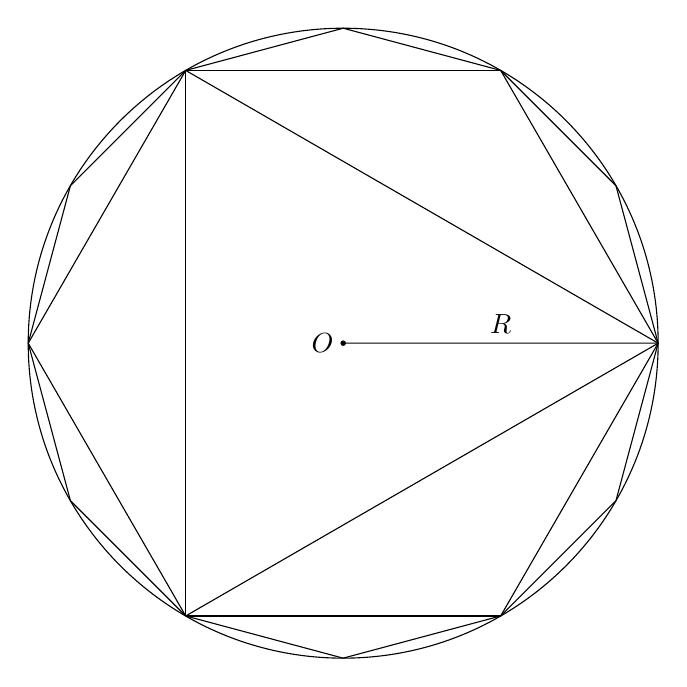
\begin{tikzpicture}
		\pgfmathsetmacro{\radius}{4}
		\def\PlotPolygon#1{
			\foreach \i in {1,...,#1}{
				\draw({\radius*cos(\i*360/#1)},{\radius*sin(\i*360/#1)})
				--({\radius*cos((\i-1)*360/#1)},{\radius*sin((\i-1)*360/#1)});
			}
		}
		\begin{scope}
			\PlotPolygon{3}
			\PlotPolygon{6}
			\PlotPolygon{12}
		\end{scope}
		\draw(0,0)circle(\radius)node[left]{\(O\)}
			--(\radius,0)node[midway,above]{\(R\)};
		\fill(0,0)circle(1pt);
	\end{tikzpicture}
	\caption{用内接正多边形覆盖圆}
	\label{figure:无穷级数.用内接正多边形覆盖圆}
\end{figure}

如果内接正多边形的边数无限增多,即\(n\)无限增大,
则和\(a_1+a_2+\dotsb+a_n\)的极限就是所要求的圆面积\(A\).
这时和式中的项数无限增多,于是出现了无穷多个数量依次相加的数学式子.

\subsection{常数项级数的概念}
\begin{definition}\label{definition:无穷级数.常数项级数的定义}
设\(\{u_n\}\)是数列.
定义:\[
	\sum_{n=1}^\infty u_n
	\defeq
	\lim_{n\to\infty} \sum_{i=1}^n u_i.
\]
我们把\(\sum_{n=1}^\infty u_n\)
称为\DefineConcept{常数项无穷级数}(infinite series with constant terms),
简称\DefineConcept{常数项级数},
或者进一步简称为\DefineConcept{级数};
把\(u_n\)称为
“级数\(\sum_{n=1}^\infty u_n\)的\DefineConcept{一般项}”;
把\(\sum_{i=1}^n u_i\)称为
“级数\(\sum_{n=1}^\infty u_n\)的\DefineConcept{部分和}(partial sum)”.

如果级数\(\sum_{n=1}^\infty u_n\)的
部分和\(\sum_{i=1}^n u_i\)
构成的数列收敛于\(s\),
则称“级数\(\sum_{n=1}^\infty u_n\) \DefineConcept{收敛}(converge)”,
我们把极限\(s\)叫做“级数\(\sum_{n=1}^\infty u_n\)的\DefineConcept{和}(sum)”;
反之,如果这个级数的部分和数列发散,
则称“级数\(\sum_{n=1}^\infty u_n\) \DefineConcept{发散}(diverge)”.

当级数收敛时,
我们把收敛级数的和\(s\)与级数的部分和\(\sum_{i=1}^n u_i\)的差值\[
	\sum_{n=1}^\infty u_n - \sum_{i=1}^n u_i
\]
叫做“级数\(\sum_{n=1}^\infty u_n\)的\DefineConcept{余项}”.
\end{definition}

\begin{example}\label{example:无穷级数.等比级数的收敛性}
%@see: 《数学分析(第二版 下册)》(陈纪修) P2 例9.1.1
级数\(\sum_{n=0}^\infty q^n\)
叫做\DefineConcept{等比级数}或\DefineConcept{几何级数}.
我们把常数\(q\)叫做“级数\(\sum_{n=0}^\infty q^n\)的\DefineConcept{公比}”.
试讨论上述等比级数的收敛性.
\begin{solution}
根据\(q\)的取值范围,分情况讨论.
\begin{enumerate}
	\item 当\(q = 1\)时,则部分和为\[
		\sum_{i=0}^n q^n
		= n,
	\]
	那么\(\lim_{n\to\infty} \sum_{i=0}^n q^n
	= \lim_{n\to\infty} n
	= \infty\),
	即级数发散.

	\item 当\(q \neq 1\),
	根据\cref{theorem:等比数列.前n项和} 有\[
		\sum_{i=0}^n q^n
		= \frac{1-q^n}{1-q}
		= \frac{1}{1-q} - \frac{q^n}{1-q}.
	\]
	\begin{enumerate}
		\item 当\(\abs{q} < 1\)时,
		由于\(\lim_{n\to\infty} q^n=0\),
		从而\(\lim_{n\to\infty} \sum_{i=0}^n q^n
		=\frac{a}{1-q}\),
		因此级数收敛,
		其和为\(\frac{a}{1-q}\).

		\item 当\(\abs{q} > 1\)时,
		由于\(\lim_{n\to\infty} q^n=\infty\),
		从而\(\lim_{n\to\infty} \sum_{i=0}^n q^n
		=\infty\),
		级数发散.

		\item 当\(q = -1\)时,部分和为\[
			\sum_{i=0}^n q^n
			= \begin{cases}
				1, & \text{\(n\)是偶数}, \\
				0, & \text{\(n\)是奇数}.
			\end{cases}
		\]
		根据\cref{theorem:子列极限.数列收敛的充分必要条件},
		\(\sum_{i=0}^n q^n\)的极限不存在,级数发散.
	\end{enumerate}
\end{enumerate}

综上所述,{\color{red}当\(\abs{q} < 1\)时,几何级数收敛;
当\(\abs{q} \geq 1\)时,几何级数发散.}
\end{solution}
\end{example}

\begin{example}\label{example:无穷级数.等差级数的收敛性}
试证级数\[
	1+2+3+\dotsb+n+\dotsb
\]是发散的.
\begin{proof}
级数的部分和为\[
	s_n = 1+2+3+\dotsb+n = \frac{n(n+1)}{2}.
\]
显然,\(\lim_{n\to\infty} s_n=\infty\),级数是发散的.
\end{proof}
\end{example}
从上例也可看出:
\begin{proposition}
除非初项\(a_0\)与公差\(d\)都等于\(0\),
否则等差级数\(\sum_{n=0}^\infty(a_0+nd)\)总是发散的.
\end{proposition}

\begin{example}
判定无穷级数\[
\frac{1}{1\cdot2}+\frac{1}{2\cdot3}+\dotsb+\frac{1}{n(n+1)}+\dotsb
\]的收敛性.
\begin{solution}
记\[
	u_n = \frac{1}{n(n+1)} = \frac{1}{n}-\frac{1}{n+1},
\]
因此\begin{align*}
	s_n &= \frac{1}{1\cdot2}+\frac{1}{2\cdot3}+\dotsb+\frac{1}{n(n+1)} \\
	&= \left(1-\frac{1}{2}\right)+\left(\frac{1}{2}-\frac{1}{3}\right)
	+\dotsb+\left(\frac{1}{n}-\frac{1}{n+1}\right) \\
	&= 1-\frac{1}{n+1}.
\end{align*}
从而\[
	\lim_{n\to\infty} s_n
	= \lim_{n\to\infty} \left(1-\frac{1}{n+1}\right)
	= 1,
\]
即该级数收敛,它的和为\(1\).
\end{solution}
\end{example}

\subsection{级数收敛的必要条件}
\begin{proposition}[级数收敛的必要条件]\label{theorem:无穷级数.级数收敛的必要条件}
%@see: 《高等数学(第六版 上册)》 P253 性质5(级数收敛的必要条件)
%@see: 《数学分析(第二版 上册)》(陈纪修) P3 定理9.1.1(级数收敛的必要条件)
如果级数\(\sum_{n=1}^\infty u_n\)收敛,
则它的一般项\(u_n\)收敛于\(0\),
即\[
	\lim_{n\to\infty} u_n = 0.
\]
\begin{proof}
设级数\(\sum_{n=1}^\infty u_n\)的部分和为\(s_n\),
且\(\lim_{n\to\infty} s_n = s\),
则\[
	\lim_{n\to\infty} u_n
	= \lim_{n\to\infty}(s_n - s_{n-1})
	= \lim_{n\to\infty} s_n - \lim_{n\to\infty} s_{n-1}
	= s - s
	= 0.
	\qedhere
\]
\end{proof}
\end{proposition}

\begin{corollary}\label{theorem:无穷级数.级数收敛的必要条件.推论}
%@see: 《高等数学(第六版 上册)》 P253
如果级数\(\sum_{n=1}^\infty u_n\)的一般项不收敛于\(0\),
即\(\lim_{n\to\infty} u_n \neq 0\),
那么\(\sum_{n=1}^\infty u_n\)发散.
\begin{proof}
\cref{theorem:无穷级数.级数收敛的必要条件} 的逆否命题.
\end{proof}
\end{corollary}

\begin{example}
%@see: 《高等数学(第六版 上册)》 P253
级数\[
	\frac12-\frac23+\frac34-\dotsb+(-1)^{n-1}\frac{n}{n+1}+\dotsb,
\]的一般项\(u_n = (-1)^{n-1} \frac{n}{n+1}\)
当\(n\to\infty\)时不趋于零,
由\cref{theorem:无穷级数.级数收敛的必要条件.推论} 可知,该级数是发散的.
\end{example}

值得注意的是,级数的一般项趋于零并不是级数收敛的充分条件.
有些级数虽然一般项趋于零,但仍然是发散的.
\begin{example}\label{example:无穷级数.调和级数的敛散性}
试证:调和级数\[
%@see: 《高等数学(第六版 上册)》 P253 (5)
	\sum_{n=1}^\infty u_n
	= 1+\frac12+\frac13+\dotsb+\frac1n+\dotsb
\]是发散的.
\begin{proof}
虽然调和级数的一般项\(\lim_{n\to\infty} u_n
= \lim_{n\to\infty} 1/n
= 0\),
但是它是发散的.
现在我们用反证法证明.

假设级数\(\sum_{n=1}^\infty u_n\)收敛.
设级数的部分和为\(s_n\),
且\(\lim_{n\to\infty} s_n
= s\).
显然,对级数\(\sum_{n=1}^\infty u_n\)的部分和\(s_{2n}\)
也有\(\lim_{n\to\infty} s_{2n}
= s\).
于是\[
	\lim_{n\to\infty} {s_{2n}-s_n}
	= \lim_{n\to\infty} s_{2n} - \lim_{n\to\infty} s_n
	= s - s
	= 0.
\]
但另一方面\[
	s_{2n} - s_n
	= \frac{1}{n+1}+\frac{1}{n+2}+\dotsb+\frac{1}{2n}
	> \underbrace{\frac{1}{2n}+\frac{1}{2n}+\dotsb+\frac{1}{2n}}_{n\text{项}}
	= \frac{1}{2},
\]\[
	\lim_{n\to\infty} {s_{2n}-s_n}
	\neq 0,
\]与假设矛盾,说明级数\(\sum_{n=1}^\infty u_n\)必定发散.
\end{proof}
\end{example}

\subsection{收敛级数的基本性质}
\begin{property}\label{theorem:无穷级数.收敛级数性质1}
%@see: 《高等数学(第六版 上册)》 P251 性质1
%@see: 《数学分析(第二版 上册)》(陈纪修) P4 定理9.1.2(线性性)
如果级数\(\sum_{n=1}^\infty u_n\)收敛于和\(s\),
则级数\(\sum_{n=1}^\infty k u_n\)收敛于和\(ks\).
\begin{proof}
设级数\(\sum_{n=1}^\infty u_n\)
与级数\(\sum_{n=1}^\infty k u_n\)的
部分和分别为\(s_n\)与\(\sigma_n\),
则\[
	\sigma_n
	= k u_1 + k u_2 + \dotsb + k u_n
	= k(u_1 + u_2 + \dotsb + u_n) = k s_n,
\]\[
	\lim_{n\to\infty} \sigma_n
	= \lim_{n\to\infty} k s_n
	= k \lim_{n\to\infty} s_n = ks,
\]
也就是说,级数\(\sum_{n=1}^\infty k u_n\)收敛于\(ks\).

特别地,对于任意发散级数\(\sum_{n=1}^\infty u_n\),
级数\(\sum_{n=1}^\infty 0 \cdot u_n\)的每一项都是零,
故级数\(\sum_{n=1}^\infty 0 \cdot u_n\)收敛于\(0\).
\end{proof}
\end{property}

由关系式\(\sigma_n = k s_n\)知道,
如果\(\{s_n\}\)没有极限且\(k\neq0\),
那么\(\{\sigma_n\}\)也不可能有极限.
因此我们得到如下结论:
{\color{red}级数的每一项同乘一个非零常数后,它的敛散性不会改变.}

\begin{example}
判断\[
\sin\frac{\pi}{6}+\sin\frac{2\pi}{6}+\dotsb+\sin\frac{n\pi}{6}+\dotsb
\]的收敛性.
\begin{solution}
记\(u_n = \sin\frac{n\pi}{6},
v_n = 2\sin\frac{\pi}{12} \cdot u_n\).
因为\[
	v_n = \cos\frac{\pi-2n\pi}{12} - \cos\frac{\pi+2n\pi}{12},
\]\[
	\sigma_n
	= v_1 + v_2 + \dotsb + v_n
	= \cos\frac{\pi}{12} - \cos\frac{(2n+1)\pi}{12},
\]
所以\[
	s_n
	= \left(2\sin\frac{\pi}{12}\right)^{-1} \cdot \sigma_n
	= 1+\frac{\sqrt{3}}{2} - \frac{\sqrt{2}}{\sqrt{3}-1} \cos\frac{(2n+1)\pi}{12}.
\]
可见\(\lim_{n\to\infty} s_n\)不存在,级数发散.
\end{solution}
\end{example}

\begin{property}\label{theorem:无穷级数.收敛级数性质2}
%@see: 《高等数学(第六版 上册)》 P251 性质2
%@see: 《数学分析(第二版 上册)》(陈纪修) P4 定理9.1.2(线性性)
如果级数\(\sum_{n=1}^\infty u_n\)、\(\sum_{n=1}^\infty v_n\)
分别收敛于\(s\)、\(\sigma\),
则级数\(\sum_{n=1}^\infty(u_n \pm v_n)\)收敛于\(s \pm \sigma\).
\begin{proof}
设级数\(\sum_{n=1}^\infty u_n\)与级数\(\sum_{n=1}^\infty v_n\)的部分和
分别为\(s_n\)与\(\sigma_n\),
则级数\(\sum_{n=1}^\infty(u_n \pm v_n)\)的部分和\begin{align*}
	\tau_n &= (u_1 \pm v_1) + (u_2 \pm v_2) + \dotsb + (u_n + v_n) \\
	&= (u_1 + u_2 + \dotsb + u_n) \pm (v_1 + v_2 + \dotsb + v_n) \\
	&= s_n \pm \sigma_n,
\end{align*}
于是\[
	\lim_{n\to\infty} \tau_n
	= \lim_{n\to\infty} (s_n \pm \sigma_n)
	= s + \sigma.
\]

这就表明级数\(\sum_{n=1}^\infty(u_n \pm v_n)\)收敛于\(s \pm \sigma\).
\end{proof}
\end{property}
\cref{theorem:无穷级数.收敛级数性质2} 也可以说成:
{\color{red}两个收敛级数可以逐项相加、逐项相减.}

\begin{example}
设级数\(\sum_{n=1}^\infty u_n\)收敛,\(\sum_{n=1}^\infty v_n\)发散.
试证:级数\(\sum_{n=1}^\infty (u_n \pm v_n)\)发散.
\begin{proof}
设级数\(\sum_{n=1}^\infty u_n\)与\(\sum_{n=1}^\infty v_n\)的部分和
分别为\(s_n\)和\(\sigma_n\),
又设\[
	\lim_{n\to\infty} s_n = s.
\]
假设级数\(\sum_{n=1}^\infty (u_n \pm v_n)\)收敛,
且\[
	\lim_{n\to\infty} (s_n \pm \sigma_n) = s+\sigma,
\]
那么根据\hyperref[theorem:极限.极限的四则运算法则]{极限的四则运算法则},
有\[
	\lim_{n\to\infty} \pm\sigma_n
	= \lim_{n\to\infty} [(s_n \pm \sigma_n) - s_n]
	= \lim_{n\to\infty} (s_n \pm \sigma_n) - \lim_{n\to\infty} s_n
	= (s + \sigma) - s
	= \sigma,
\]
也就是说\(\{\pm\sigma_n\}\)(即\(\pm\sum_{n=1}^\infty v_n\))收敛,矛盾!
\end{proof}
\end{example}

从上例我们可以看出:
\begin{proposition}\label{theorem:无穷级数.收敛级数性质2.推论1}
一个收敛级数与一个发散级数相加(或相减)所得级数必定发散.
\end{proposition}

另一方面,任给一个发散级数\(\sum_{n=1}^\infty u_n\),
级数\(\sum_{n=1}^\infty u_n + \sum_{n=1}^\infty u_n
= \sum_{n=1}^\infty 2 u_n\)也是发散的,
而级数\(\sum_{n=1}^\infty u_n - \sum_{n=1}^\infty u_n
= 0\)却是收敛的,
于是我们还可以看出:
{\color{red}两个发散级数相加(或相减)所得级数可能收敛也可能发散.}

\begin{example}
已知级数\(\sum_{n=1}^\infty (-1)^{n-1} a_n = 2,
\sum_{n=1}^\infty a_{2n-1} = 5\),
求\(\sum_{n=1}^\infty a_n\).
\begin{solution}
由于\(\sum_{n=1}^\infty [a_n + (-1)^{n-1} a_n]
= 2 \sum_{n=1}^\infty a_{2n-1}\)收敛,
所以\(\sum_{n=1}^\infty a_n\)收敛,且有
\[
\sum_{n=1}^\infty a_n
= 2 \sum_{n=1}^\infty a_{2n-1}
- \sum_{n=1}^\infty (-1)^{n-1} a_n
= 10 - 2 = 8.
\]
\end{solution}
\end{example}

\begin{property}\label{theorem:无穷级数.收敛级数性质3}
%@see: 《高等数学(第六版 上册)》 P252 性质3
在级数中去掉、加上或改变有限项,不会改变级数的收敛性.
\begin{proof}
我们只需证明“在级数的前面部分去掉或加上有限项,不会改变级数的收敛性”,
因为其他情形(即在级数中任意去掉、加上或改变有限项的情形)都可以看成在级数的前面部分先去掉有限项,
然后再加上有限项的结果.

将级数\[
u_1+u_2+\dotsb+u_k+u_{k+1}+\dotsb+u_{k+n}+\dotsb
\]的前\(k\)项去掉,则得级数\[
u_{k+1}+u_{k+2}+\dotsb+u_{k+n}+\dotsb.
\]于是新得到的级数的部分和为\[
\sigma_n = u_{k+1}+u_{k+2}+\dotsb+u_{k+n} = s_{k+n} - s_k,
\]其中\(s_{k+n}\)是原级数的前\(k+n\)项的和.
因为\(s_k\)是常数,所以当\(n\to\infty\)时,
\(\sigma_n\)与\(s_{k+n}\)这两个量,要么同时具有极限,要么同时没有极限.

同理可证在级数的前面加上有限项,不会改变级数的收敛性.
由此可见,在级数中去掉、加上或改变有限项,不会改变级数的收敛性.

另外,我们可以观察到,在收敛级数中去掉、加上或改变有限项,
虽不会改变级数的收敛性,但可能会改变收敛级数的和.
\end{proof}
\end{property}

\begin{property}\label{theorem:无穷级数.收敛级数性质4}
%@see: 《高等数学(第六版 上册)》 P252 性质4
%@see: 《数学分析(第二版 上册)》(陈纪修) P4 定理9.1.3
如果级数\(\sum_{n=1}^\infty u_n\)收敛,
则对这级数的项任意加括号后所成的级数\[
%@see: 《高等数学(第六版 上册)》 P252 (4)
	(u_1+\dotsb+u_{n_1})
	+ (u_{n_1+1}+\dotsb+u_{n_2})
	+ \dotsb
	+ (u_{n_{k-1}+1}+\dotsb+u_{n_k}) + \dotsb
\]仍收敛,且其和不变.
\end{property}

应该注意到:
如果加括号后所成的级数收敛,则不能断定去括号后原来的级数也收敛.
例如,级数\[
	(1-1)+(1-1)+\dotsb
\]收敛于零,
但级数\[
	1-1+1-1+\dotsb
\]却是发散的.

根据\cref{theorem:无穷级数.收敛级数性质4} 可得如下推论:
{\color{red}如果加括号后所成的级数发散,则原来的级数也发散.}
事实上,倘若原级数收敛,
则根据\cref{theorem:无穷级数.收敛级数性质4} 知道,
加括号后的级数就应该收敛了.

\subsection{柯西审敛原理}
由于无穷级数\(\sum_{n=1}^\infty u_n\)收敛
即为极限\(\lim_{n\to\infty} \sum_{k=1}^n u_k\)存在,
对无穷级数收敛性的最本质的刻画,
就是极限论中的\hyperref[theorem:极限.函数的柯西极限存在准则]{柯西极限存在准则},
它可以表述为如下形式:
\begin{theorem}[柯西审敛原理]\label{theorem:无穷级数.级数的柯西审敛原理}
%@see: 《高等数学(第六版 下册)》 P254 柯西审敛原理
%@see: 《数学分析(第二版 下册)》(陈纪修) P29 定理9.4.1(级数的Cauchy收敛原理)
%@see: 《数学分析教程(第3版 下册)》(史济怀) P180 定理14.4.1(Cauchy收敛原理)
级数\(\sum_{n=1}^\infty u_n\)收敛的充分必要条件为:
对于任意给定的正数\(\epsilon\),
总存在正整数\(N\),
使得当\(n>N\)时,
对于任意的正整数\(m\),
总是成立\[
	\abs{ \sum_{k=1}^m u_{n+k} }
	< \epsilon.
\]
\end{theorem}

我们可以利用极限记号,
把\hyperref[theorem:无穷级数.级数的柯西审敛原理]{柯西审敛原理}改写为如下命题.
\begin{proposition}
级数\(\sum_{n=1}^\infty u_n\)收敛的充分必要条件是:
对于任意正整数\(m\),总有\[
	\lim_{n\to\infty} \sum_{k=1}^m u_{n+k} = 0.
\]
\end{proposition}

\begin{example}
试求级数\(\sum_{n=1}^\infty \frac{1}{n^2}\)的收敛性.
\begin{solution}
因为对任意正整数\(p\),\begin{align*}
	&\abs{u_{n+1}+u_{n+2}+\dotsb+u_{n+p}} \\
	&=\frac{1}{(n+1)^2}+\frac{1}{(n+2)^2}+\dotsb+\frac{1}{(n+p)^2} \\
	&<\frac{1}{n(n+1)}+\frac{1}{(n+1)(n+2)}+\dotsb+\frac{1}{(n+p-1)(n+p)} \\
	&=\left(\frac{1}{n}-\frac{1}{n+1}\right)
		+\left(\frac{1}{n+1}-\frac{1}{n+2}\right)
		+\dotsb+\left(\frac{1}{n+p-1}-\frac{1}{n+p}\right) \\
	&=\frac{1}{n}-\frac{1}{n+p} < \frac{1}{n},
\end{align*}
所以对于\(\forall \epsilon > 0\),
取正整数\(N \geq \frac{1}{\epsilon}\),
则当\(n > N\)时,
对任何正整数\(p\),
都有\[
	\abs{u_{n+1}+u_{n+2}+\dotsb+u_{n+p}}
	< \frac{1}{n}
	< \frac{1}{N}
	\leq \epsilon
\]成立.
按柯西审敛原理,级数\(\sum_{n=1}^\infty \frac{1}{n^2}\)收敛.
\end{solution}
\end{example}

\section{常数项级数的审敛法}
%@see: [19世纪上半叶的无穷级数敛散性判别法(华东师范大学数学系,汪晓勤)](https://faculty.ecnu.edu.cn/picture/article/1284/f3/48/968f8e4243b885767e11fcf63faf/5e2f0d6b-5780-4ad8-92d3-7cf2516e7083.pdf.x)
\subsection{正项级数及其审敛法}
\subsubsection{正项级数的概念及其收敛条件}
一般的常数项级数,它的各项可以是正数、负数或零.
现在我们先讨论各项都是正数或零的级数,这种级数称为\DefineConcept{正项级数}.
这种级数特别重要,以后将看到许多级数的收敛性问题可归结为正项级数的收敛性问题.

\begin{theorem}\label{theorem:无穷级数.正项级数收敛的充分必要条件}
%@see: 《高等数学(第六版 下册)》 P256 定理1
%@see: 《数学分析教程 (第3版 下册)》 P163 定理14.2.1
%@see: 《数学分析(第二版 下册)》(陈纪修) P16 定理9.3.1(正项级数的收敛原理)
正项级数收敛的充分必要条件是:它的部分和数列有界.
\begin{proof}
设\(\sum_{n=1}^\infty u_n\)是一个正项级数,
它的部分和数列为\(\{s_n\}\).
显然,数列\(\{s_n\}\)是一个单调增加数列.
如果数列\(\{s_n\}\)有界,
那么根据\hyperref[theorem:极限.数列的单调有界定理]{单调有界定理},
数列\(\{s_n\}\)收敛,
也就是说,级数\(\sum_{n=1}^\infty u_n\)收敛.

反之,如果正项级数\(\sum_{n=1}^\infty u_n\)收敛于和\(s\),
即\(\lim_{n\to\infty} s_n = s\),
根据\hyperref[theorem:极限.收敛数列的有界性]{收敛数列的有界性}可知,
数列\(\{s_n\}\)有界.
\end{proof}
\end{theorem}

我们可以写出\cref{theorem:无穷级数.正项级数收敛的充分必要条件} 的逆否命题.
\begin{proposition}
%@see: 《数学分析(第二版 下册)》(陈纪修) P16 定理9.3.1(正项级数的收敛原理)
正项级数发散的充分必要条件是:它的部分和数列无界.
\end{proposition}

\begin{example}
%@see: 《数学分析教程 (第3版 下册)》 P163 例1
设正项级数\(\sum_{n=1}^\infty a_n\)的部分和是\(s_n\),证明:\[
	\sum_{n=1}^\infty \frac{a_n}{s_n^2} < +\infty.
\]
\begin{proof}
显然\(\sum_{n=1}^\infty \frac{a_n}{s_n^2}\)是正项级数.
由于对于任意正整数\(N\),有\begin{align*}
	\sum_{n=2}^N \frac{a_n}{s_n^2}
	&= \sum_{n=2}^N \frac{s_n-s_{n-1}}{s_n^2}
	\leq \sum_{n=2}^N \frac{s_n-s_{n-1}}{s_{n-1} s_n} \\
	&= \sum_{n=2}^N \left(
			\frac{1}{s_{n-1}} - \frac{1}{s_n}
		\right)
	= \frac{1}{s_1} - \frac{1}{s_N}
	< \frac{1}{a_1},
\end{align*}
也就是说\(\sum_{n=1}^\infty \frac{a_n}{s_n^2}\)的部分和有界,
所以根据\cref{theorem:无穷级数.正项级数收敛的充分必要条件},该级数收敛.
\end{proof}
\end{example}

\subsubsection{比较审敛法}
利用\cref{theorem:无穷级数.正项级数收敛的充分必要条件} 直接证明某些级数的部分和有界不太容易,
因此我们需要一个判别级数敛散性的更简单的方法.

\begin{theorem}[比较审敛法]\label{theorem:无穷级数.正项级数的比较审敛法}
%@see: 《高等数学(第六版 下册)》 P256 定理2
%@see: 《数学分析教程 (第3版 下册)》 P164 定理14.2.2
设\(\sum_{n=1}^\infty u_n\)
和\(\sum_{n=1}^\infty v_n\)都是正项级数,且\[
	u_n \leq v_n
	\quad(n=1,2,\dotsc).
\]
若级数\(\sum_{n=1}^\infty v_n\)收敛,
则级数\(\sum_{n=1}^\infty u_n\)收敛;
反之,若级数\(\sum_{n=1}^\infty u_n\)发散,
则级数\(\sum_{n=1}^\infty v_n\)发散.
\begin{proof}
设级数\(\sum_{n=1}^\infty v_n\)收敛于和\(\sigma\),
则级数\(\sum_{n=1}^\infty u_n\)的部分和\[
	s_n = u_1 + u_2 + \dotsb u_n
	\leq
	v_1 + v_2 + \dotsb + v_n \leq \sigma
	\quad(n=1,2,\dotsc),
\]
即部分和数列\(\{s_n\}\)有界,
由\cref{theorem:无穷级数.正项级数收敛的充分必要条件} 知级数\(\sum_{n=1}^\infty u_n\)收敛.
\end{proof}
\end{theorem}

\begin{example}
判断级数\(\sum_{n=1}^\infty \frac{1}{1+a^n}\ (a>0)\)的收敛性.
\begin{solution}
显然有\[
	\frac{1}{1+a^n} < \frac{1}{a^n}.
\]
根据比较审敛法,如果级数\(\sum_{n=1}^\infty \frac{1}{a^n}\)收敛,
那么级数\(\sum_{n=1}^\infty \frac{1}{1+a^n}\)收敛;
而等比级数\(\sum_{n=1}^\infty \frac{1}{a^n}\)
当且仅当其公比\(\abs{\frac{1}{a}} < 1\),即\(a > 1\)时收敛;
故当\(a > 1\)时,级数\(\sum_{n=1}^\infty \frac{1}{1+a^n}\)收敛.

当\(0 < a \leq 1\)时,\(0 < a^n \leq 1\),\(1 < 1 + a^n \leq 2\),\[
	\frac{1}{1+a^n} \geq \frac{1}{2},
\]
而等差级数\(\sum_{n=1}^\infty \frac{1}{2}\)发散,
故级数\(\sum_{n=1}^\infty \frac{1}{1+a^n}\)发散.
\end{solution}
\end{example}

注意到级数的每一项同乘不为零的常数\(k\)
以及去掉级数前面部分的有限项不会影响级数的收敛性,
我们可得如下推论:
\begin{corollary}\label{theorem:无穷级数.正项级数的比较审敛法的推论}
%@see: 《高等数学(第六版 下册)》 P257 推论
%@see: 《数学分析(第二版 下册)》(陈纪修) P17 定理9.3.2(比较判别法)
设\(\sum_{n=1}^\infty u_n\)和\(\sum_{n=1}^\infty v_n\)都是正项级数.
\begin{itemize}
	\item 如果级数\(\sum_{n=1}^\infty v_n\)收敛,
	且从某一项开始\(u_n\)小于或等于\(v_n\)的正倍数,
	即\[
		(\exists k>0)
		(\exists N\in\mathbb{N})
		(\forall n\in\mathbb{N})
		[
			n > N
			\implies
			u_n \leq k v_n
		],
	\]
	则级数\(\sum_{n=1}^\infty u_n\)收敛.

	\item 如果级数\(\sum_{n=1}^\infty v_n\)发散,
	且从某一项开始\(u_n\)大于或等于\(v_n\)的正倍数,
	即\[
		(\exists k>0)
		(\exists N\in\mathbb{N})
		(\forall n\in\mathbb{N})
		[
			n > N
			\implies
			u_n \geq k v_n
		],
	\]
	则级数\(\sum_{n=1}^\infty u_n\)发散.
\end{itemize}
\end{corollary}

\begin{example}
%@see: 《高等数学(第六版 下册)》 P257 例2
试证:级数\(\sum_{n=1}^\infty \frac{1}{\sqrt{n(n+1)}}\)是发散的.
\begin{proof}
因为\(n(n+1) < (n+1)^2\),所以\(\frac{1}{\sqrt{n(n+1)}} > \frac{1}{n+1}\),而级数\(\sum_{n=1}^\infty \frac{1}{n+1}\)是发散的,根据比较审敛法可知级数\(\sum_{n=1}^\infty \frac{1}{\sqrt{n(n+1)}}\)是发散的.
\end{proof}
\end{example}

\subsubsection{\texorpdfstring{\(p\)}{p}级数}
\begin{proposition}\label{example:无穷级数.p级数的收敛性}
%@see: 《高等数学(第六版 下册)》 P257 例1
讨论\(p\)级数\[
	1+\frac{1}{2^p}+\frac{1}{3^p}+\dotsb+\frac{1}{n^p}+\dotsb
\]的收敛性,
其中常数\(p>0\).
\begin{solution}
当\(p \leq 1\)时,\(p\)级数各项均不小于调和级数对应项,
即\(\frac{1}{n^p} \geq \frac{1}{n}\),
但调和级数发散,
故根据\cref{theorem:无穷级数.正项级数的比较审敛法} 可知,
当\(p \leq 1\)时\(p\)级数发散.

当\(p > 1\)时,
因为\(k-1
\leq x
\leq k \implies \frac{1}{k}
\leq \frac{1}{x} \implies \frac{1}{k^p}
\leq \frac{1}{x^p}\),
所以\[
	\frac{1}{k^p}
	= \int_{k-1}^k \frac{1}{k^p} \dd{x}
	\leq \int_{k-1}^k \frac{1}{x^p} \dd{x}
	\quad(k=2,3,\dotsc),
\]
从而级数的部分和
\begin{align*}
	s_n &= 1 + \sum_{k=2}^n{\frac{1}{k^p}}
	\leq 1 + \sum_{k=2}^n{ \int_{k-1}^k{\frac{1}{x^p}\dd{x}} }
	= 1 + \int_1^n{\frac{1}{x^p}\dd{x}} \\
	&= 1 + \frac{1}{p-1}\left(1-\frac{1}{n^{p-1}}\right)
	< 1 + \frac{1}{p-1}
	\quad(n=2,3,\dotsc),
\end{align*}
这表明数列\(\{s_n\}\)有界,因此\(p\)级数收敛.

综上所述,{\color{red} \(p\)级数\(\sum_{n=1}^\infty \frac{1}{n^p}\)
当\(p > 1\)时收敛,
当\(p \leq 1\)时发散.}
\end{solution}
\end{proposition}
可以发现,\(p\)级数与
\hyperref[example:定积分.p积分]{\(p\)积分}具有高度相似性.

\begin{example}
设正项级数\(\sum_{n=1}^\infty a_n\)的部分和是\(s_n\),
证明:对于任意\(k>1\),有\[
	\sum_{n=1}^\infty \frac{a_n}{s_n^k} < +\infty.
\]
\begin{proof}
当\(k>1\)时,
有\begin{align*}
	\sum_{i=2}^n \frac{a_i}{s_i^k}
	&= \sum_{i=2}^n \frac{s_i-s_{i-1}}{s_i^k} \\
	&= \sum_{i=2}^n \frac{1}{s_i^k} \int_{s_{i-1}}^{s_i} \dd{x}
			\tag{\cref{theorem:定积分.定积分性质4}} \\
	&\leq \sum_{i=2}^n \int_{s_{i-1}}^{s_i} \frac{\dd{x}}{x^k}
			\tag{\cref{theorem:定积分.定积分性质6}} \\
	&= \int_{s_1}^{s_n} \frac{\dd{x}}{x^k}
			\tag{\cref{theorem:定积分.定积分性质3}} \\
	&\leq \int_{s_1}^{+\infty} \frac{\dd{x}}{x^k}
	< +\infty,
			\tag{\cref{example:定积分.p积分}}
\end{align*}
可见该级数的部分和有界,因此该级数收敛.
\end{proof}
\end{example}

\begin{example}
设正项级数\(\sum_{n=1}^\infty a_n\)发散,证明:级数\(\sum_{n=1}^\infty \frac{a_n}{n^3+a_n^2}\)收敛.
\begin{proof}
由基本不等式 \labelcref{theorem:不等式.基本不等式2} 可知
\(n^3+a_n^2\geq2\sqrt{n^3 a_n^2}=2n^{3/2}a_n\),
那么\(\frac{a_n}{n^3+a_n^2}\leq\frac{a_n}{2n^{3/2}a_n}=\frac{1}{2n^{3/2}}\).
由\cref{example:无穷级数.p级数的收敛性}
我们知道\(p=\frac{3}{2}>1\)时,\(p\)级数收敛;
那么根据\hyperref[theorem:无穷级数.正项级数的比较审敛法]{比较审敛法}可知
级数\(\sum_{n=1}^\infty \frac{a_n}{n^3+a_n^2}\)收敛.
\end{proof}
\end{example}

\subsubsection{比较审敛法的极限形式}
\begin{theorem}[比较审敛法的极限形式]\label{theorem:无穷级数.正项级数的比较审敛法的极限形式}
%@see: 《高等数学(第六版 下册)》 P258 定理3
%@see: 《数学分析(第二版 下册)》(陈纪修) P18 定理9.3.2'(比较判别法的极限形式)
设\(\sum_{n=1}^\infty u_n\)和\(\sum_{n=1}^\infty v_n\)都是正项级数,
记\[
	\rho
	\defeq
	\lim_{n\to\infty} \frac{u_n}{v_n}.
\]
\begin{itemize}
	\item 如果\(\rho\in[0,+\infty)\),
	且级数\(\sum_{n=1}^\infty v_n\)收敛,
	则级数\(\sum_{n=1}^\infty u_n\)收敛.

	\item 如果\(\rho\in(0,+\infty]\),
	且级数\(\sum_{n=1}^\infty v_n\)发散,
	则级数\(\sum_{n=1}^\infty u_n\)发散.
\end{itemize}
\begin{proof}
如果\(\rho\in[0,+\infty)\),
那么由极限定义可知,
对\(\epsilon=1\),
存在正整数\(N\),
当\(n>N\)时,
有\[
	\frac{u_n}{v_n} < l+1,
\]
即\(u_n < (l+1) v_n\).
而级数\(\sum_{n=1}^\infty v_n\)收敛,
根据\cref{theorem:无穷级数.正项级数的比较审敛法的推论} 可知,
级数\(\sum_{n=1}^\infty u_n\)收敛.

如果\(\rho\in(0,+\infty]\),
那么极限\(\lim_{n\to\infty} \frac{v_n}{u_n}\)存在且有限.
如果级数\(\sum_{n=1}^\infty u_n\)收敛,
那么由上可知,级数\(\sum_{n=1}^\infty v_n\)收敛;
但已知级数\(\sum\limits{n=1}^\infty v_n\)发散,矛盾!
因此级数\(\sum_{n=1}^\infty u_n\)不可能收敛,
即级数\(\sum_{n=1}^\infty u_n\)发散.
\end{proof}
\end{theorem}

极限形式的比较审敛法,在两个正项级数的一般项均趋于零的情况下,
其实是比较它们的一般项作为无穷小量的阶.
定理表明,当\(n \to \infty\)时,
如果\(u_n\)是与\(v_n\)同阶或是比\(v_n\)高阶的无穷小,
而级数\(\sum_{n=1}^\infty v_n\)收敛,则级数\(\sum_{n=1}^\infty u_n\)收敛;
如果\(u_n\)是与\(v_n\)同阶或是比\(v_n\)低阶的无穷小,
而级数\(\sum_{n=1}^\infty v_n\)发散,则级数\(\sum_{n=1}^\infty u_n\)发散.

\begin{example}
%@see: 《高等数学(第六版 下册)》 P258 例3
判断级数\(\sum_{n=1}^\infty \sin\frac{1}{n}\)的收敛性.
\begin{solution}
因为\[
	\lim_{n\to\infty} \frac{\sin(1/n)}{1/n} = 1 > 0,
\]
而级数\(\sum_{n=1}^\infty \frac{1}{n}\)发散,
可知级数\(\sum_{n=1}^\infty \sin\frac{1}{n}\)发散.
\end{solution}
\end{example}

\begin{example}
%@see: 《高等数学(第六版 下册)》 P268 习题12-2 1. (1)
判断级数\[
	1 + \frac{1}{3} + \frac{1}{5} + \dotsb + \frac{1}{2n-1} + \dotsb
\]的收敛性.
\begin{solution}
记\(u_n = \frac{1}{2n-1}\),
取\(v_n = \frac{1}{n}\).
因为\[
	\lim_{n\to\infty} \frac{u_n}{v_n}
	= \lim_{n\to\infty} \frac{n}{2n-1}
	= \lim_{n\to\infty} \frac{1}{2-1/n}
	= \frac{1}{2}
	> 0,
\]
而级数\(\sum_{n=1}^\infty \frac{1}{n}\)发散,
所以级数\(\sum_{n=1}^\infty \frac{1}{2n-1}\)发散.
\end{solution}
\end{example}

\begin{example}
%@see: 《高等数学(第六版 下册)》 P268 习题12-2 1. (2)
判断级数\[
	1 + \frac{1+2}{1+2^2} + \frac{1+3}{1+3^2} + \dotsb + \frac{1+n}{1+n^2} + \dotsb
\]的收敛性.
\begin{solution}
记\(u_n = \frac{1+n}{1+n^2}\),
取\(v_n = \frac{1}{1+n}\).
因为\[
	\lim_{n\to\infty} \frac{u_n}{v_n}
	= \lim_{n\to\infty} \frac{(1+n)^2}{1+n^2}
	= \lim_{n\to\infty} \frac{n^2 + 2n + 1}{n^2 + 1}
	= 1 > 0,
\]
而\(\sum_{n=1}^\infty v_n\)发散,
所以级数\(\sum_{n=1}^\infty \frac{1+n}{1+n^2}\)发散.
\end{solution}
\end{example}

\begin{example}
%@see: 《高等数学(第六版 下册)》 P268 习题12-2 1. (3)
判断级数\[
	\frac{1}{2\cdot5} + \frac{1}{3\cdot6} + \dotsb + \frac{1}{(n+1)(n+4)} + \dotsb
\]的收敛性.
\begin{solution}
记\(u_n = \frac{1}{(n+1)(n+4)}\),
取\(v_n = \frac{1}{n^2}\).
因为\[
	\lim_{n\to\infty} \frac{u_n}{v_n}
	= \lim_{n\to\infty} \frac{n^2}{(n+1)(n+4)}
	= 1,
\]
而级数\(\sum_{n=1}^\infty v_n\)收敛,
所以级数\(\sum_{n=1}^\infty \frac{1+n}{1+n^2}\)收敛.
\end{solution}
\end{example}

\begin{example}
%@see: 《高等数学(第六版 下册)》 P268 习题12-2 1. (4)
\newcommand\sinfrac[1][]{\sin\frac{\pi}{2^{#1}}}
判断级数\[
	\sinfrac + \sinfrac[2] + \sinfrac[3] + \dotsb + \sinfrac[n] + \dotsb
\]的收敛性.
\begin{solution}
记\(u_n = \sin\frac{\pi}{2^n}\),
取\(v_n = \frac{\pi}{2^n}\).
因为\[
	\lim_{n\to\infty} \frac{u_n}{v_n}
	= \lim_{n\to\infty} \frac{\sin(\pi/2^n)}{\pi/2^n}
	= 1,
\]
而级数\(\sum_{n=1}^\infty v_n\)收敛,
所以级数\(\sum_{n=1}^\infty \sin\frac{\pi}{2^n}\)收敛.
\end{solution}
\end{example}

\begin{example}
%@see: 《数学分析(第二版 下册)》(陈纪修) P19 例9.3.4
判断正项级数\(\sum_{n=1}^\infty \left(\exp\frac1{n^2}-\cos\frac\pi{n}\right)\)的敛散性.
\begin{solution}
因为\begin{align*}
	\exp\frac1{n^2}-\cos\frac\pi{n}
	&= \left[1+\frac1{n^2}+o\left(\frac1{n^2}\right)\right]
	- \left[1-\frac12\left(\frac\pi{n}\right)^2+o\left(\frac1{n^2}\right)\right] \\
	&= \left(1+\frac{\pi^2}2\right) \frac1{n^2} + o\left(\frac1{n^2}\right),
\end{align*}
所以\[
	\lim_{n\to\infty} n^2 \left(\exp\frac1{n^2}-\cos\frac\pi{n}\right)
	= 1+\frac{\pi^2}2.
\]
由于\(\sum_{n=1}^\infty \frac1{n^2}\)收敛,
所以\(\sum_{n=1}^\infty \left(\exp\frac1{n^2}-\cos\frac\pi{n}\right)\)收敛.
\end{solution}
\end{example}

\subsubsection{比值审敛法}
用比较审敛法审敛时,
需要适当地选取一个已知其收敛性的级数\(\sum_{n=1}^\infty v_n\)作为比较的基准.
最常选用作为基准级数的是正项等比级数\(\sum_{n=1}^\infty q^n\ (q>0)\)
和\(p\)级数\(\sum_{n=1}^\infty \frac1{n^p}\).

我们知道,\hyperref[example:无穷级数.等比级数的收敛性]{等比级数}
\(\sum_{n=1}^\infty q^n\)的敛散性只依赖于其相邻两项之比\(q\)是否小于\(1\).
利用\hyperref[theorem:无穷级数.正项级数的比较审敛法]{比较审敛法}可以得出以下结论:
设级数\(\sum_{n=1}^\infty u_n\)的后项与前项之比\(\frac{u_{n+1}}{u_n}\)
或前\(n\)项的“平均公比”
\(\sqrt[n]{u_n}
= \sqrt[n]{\frac{u_1}1\cdot\frac{u_2}{u_1}\dotsm\frac{u_n}{u_{n-1}}}\)
的极限是\(\rho\),
如果\(\rho<1\),那么级数\(\sum_{n=1}^\infty u_n\)收敛;
如果\(\rho>1\),那么级数\(\sum_{n=1}^\infty u_n\)发散.
正是基于这样的思路,产生了如下的\hyperref[theorem:无穷级数.正项级数的比值审敛法]{比值审敛法}%
和\hyperref[theorem:无穷级数.正项级数的根值审敛法]{根值审敛法}.

\begin{theorem}[比值审敛法,达朗贝尔判别法]\label{theorem:无穷级数.正项级数的比值审敛法}
设\(\sum_{n=1}^\infty u_n\)是正项级数,
记\(\rho \defeq \lim_{n\to\infty} \frac{u_{n+1}}{u_n}\).
\begin{itemize}
	\item 当\(\rho<1\)时,级数\(\sum_{n=1}^\infty u_n\)收敛.
	\item 当\(\rho>1\)时,或当\(\rho=\infty\)时,级数\(\sum_{n=1}^\infty u_n\)发散.
	\item 当\(\rho=1\)时,级数\(\sum_{n=1}^\infty u_n\)可能收敛也可能发散.
\end{itemize}
\begin{proof}
当\(\rho<1\).
取一个适当小的正数\(\epsilon\),
使得\(\rho+\epsilon=r<1\),
根据极限定义,
存在正整数\(m\),
当\(n \geq m\)时有不等式\[
	\frac{u_{n+1}}{u_n} < \rho + \epsilon = r.
\]
因此\[
	u_{m+1} < r u_m,
	u_{m+2} < r u_{m+1} < r^2 u_m,
	\dotsc,
	u_{m+k} < r^k u_m,
	\dotsc.
\]
而因为公比\(r<1\),
故等比级数\(\sum_{k=1}^\infty r^k u_m\)收敛,
根据\cref{theorem:无穷级数.正项级数的比较审敛法的推论} 可知,
级数\(\sum_{n=1}^\infty u_n\)收敛.

当\(\rho>1\).
取一个适当小的正数\(\epsilon\),
使得\(\rho-\epsilon>1\).
根据极限定义,
当\(n \geq m\)时有不等式\[
	\frac{u_{n+1}}{u_n} > \rho-\epsilon > 1,
\]
也就是\(u_{n+1}>u_n\).
所以当\(n \geq m\)时,
级数的一般项\(u_n\)是逐渐增大的,
从而\[
	\lim_{n\to\infty} u_n \neq 0.
\]
根据\cref{theorem:无穷级数.收敛级数性质5} (即级数收敛的必要条件)可知,
级数\(\sum_{n=1}^\infty u_n\)发散.

类似地,可以证明当\(\lim_{n\to\infty} \frac{u_{n+1}}{u_n} = \infty\)时,
级数\(\sum_{n=1}^\infty u_n\)发散.

当\(\rho = 1\)时,
级数可能收敛也可能发散.
例如\(p\)级数不论\(p\)为何值都有\[
	\lim_{n\to\infty} \frac{u_{n+1}}{u_n}
	= \lim_{n\to\infty} \frac{1/(n+1)^p}{1/n^p} = 1.
\]
但我们知道,
当\(p>1\)时\(p\)级数收敛,
当\(p\leq1\)时\(p\)级数发散,
因此只根据\(\rho=1\)不能判定级数的收敛性.
\end{proof}
\end{theorem}

\begin{example}\label{example:无穷级数.常数e的级数表示}
%@see: 《高等数学(第六版 下册)》 P260 例5
证明级数\[
	1+\frac{1}{1}+\frac{1}{1\cdot2}+\frac{1}{1\cdot2\cdot3}+\dotsb+\frac{1}{(n-1)!}+\dotsb
\]是收敛的,
并估计以级数的部分和\(s_n\)近似代替和\(s\)所产生的误差.
\begin{solution}
因为\[
	\lim_{n\to\infty} \frac{u_{n+1}}{u_n}
	 \lim_{n\to\infty} \frac{(n-1)!}{n!}
	= \lim_{n\to\infty} \frac{1}{n} = 0 < 1,
\]
根据比值审敛法可知,该级数收敛.

以该级数的部分和近似代替和\(s\)所产生的的误差为\begin{align*}
	\abs{r_n} &= \frac{1}{n!} + \frac{1}{(n+1)!} + \frac{1}{(n+2)!} + \dotsb \\
	&= \frac{1}{n!} \left[ 1 + \frac{1}{n+1} + \frac{1}{(n+1)(n+2)} + \dotsb \right] \\
	&< \frac{1}{n!} \left( 1 + \frac{1}{n} + \frac{1}{n^2} + \dotsb \right) \\
	&= \frac{1}{n!} \frac{1}{1-1/n}
	= \frac{1}{(n-1)\cdot(n-1)!}.
\end{align*}
\end{solution}
\end{example}

\begin{example}
%@see: 《高等数学(第六版 下册)》 P268 习题12-2 2. (1)
判断级数\[
	\frac{3}{1\cdot2}
	+\frac{3^2}{2\cdot2^2}
	+\frac{3^3}{3\cdot2^3}
	+\dotsb
	+\frac{3^n}{n\cdot2^n}
	+\dotsb
\]的收敛性.
\begin{solution}
记\(u_n = \frac{3^n}{n\cdot2^n}\).
因为\[
	\lim_{n\to\infty} \frac{u_{n+1}}{u_n}
	= \lim_{n\to\infty} \frac{3}{2}\cdot\frac{n}{n+1}
	= \frac{3}{2} > 1,
\]
所以级数发散.
\end{solution}
\end{example}

\begin{example}
判断级数\(\sum_{n=1}^\infty \frac{n^2}{3^n}\)的收敛性.
\begin{solution}
记\(u_n = \frac{n^2}{3^n}\).因为\[
\lim_{n\to\infty} \frac{u_{n+1}}{u_n}
= \lim_{n\to\infty} \frac{1}{3} \cdot \frac{(n+1)^2}{n^2}
= \frac{1}{3} < 1,
\]所以级数收敛.
\end{solution}
\end{example}

\begin{example}
判断级数\(\sum_{n=1}^\infty \frac{2^n \cdot n!}{n^n}\)的收敛性.
\begin{solution}
记\(u_n = \frac{2^n \cdot n!}{n^n}\).
因为\begin{align*}
	\lim_{n\to\infty} \frac{u_{n+1}}{u_n}
	&= \lim_{n\to\infty} 2(n+1) \cdot \frac{n^n}{(n+1)^{n+1}} \\
	&= 2 \cdot \lim_{n\to\infty} \frac{n^n}{(n+1)^n}
	= 2 \cdot \lim_{n\to\infty} \frac{1}{\left(1+\frac{1}{n}\right)^n} \\
	&= 2 \left[ \lim_{n\to\infty} \left(1+\frac{1}{n}\right)^n \right]^{-1}
	= \frac{2}{e} < 1,
\end{align*}
所以级数收敛.
\end{solution}
\end{example}

\begin{example}
判断级数\(\sum_{n=1}^\infty n \tan\frac{\pi}{2^{n+1}}\)的收敛性.
\begin{solution}
记\(u_n = n \tan\frac{\pi}{2^{n+1}}\).我们有\[
	\frac{u_{n+1}}{u_n}
	= \frac{n+1}{n} \frac{\tan(\frac{1}{2}\frac{\pi}{2^{n+1}})}{\tan\frac{\pi}{2^{n+1}}}.
\]
根据二倍角公式\[
	\tan2\theta = \frac{2\tan\theta}{1-\tan^2\theta},
	\qquad
	\frac{\tan\theta}{\tan2\theta} = \frac{1-\tan^2\theta}{2},
\]
有\[
	\frac{\tan(\frac{1}{2}\frac{\pi}{2^{n+1}})}{\tan\frac{\pi}{2^{n+1}}}
	= \frac{1}{2} \left(
		1-\tan^2\frac{\pi}{2^{n+2}}
	\right).
\]
于是\begin{align*}
	\lim_{n\to\infty} \frac{u_{n+1}}{u_n}
	&= \lim_{n\to\infty} \frac{n+1}{n} \frac{1}{2} \left(
		1-\tan^2\frac{\pi}{2^{n+2}}
	\right) \\
	&= \frac{1}{2} \cdot \lim_{n\to\infty} \frac{n+1}{n} \cdot \left(
		1 - \lim_{n\to\infty} \tan^2\frac{\pi}{2^{n+2}}
	\right) \\
	&= \frac{1}{2} \cdot 1 \cdot (1 - 0) = \frac{1}{2} < 1.
\end{align*}
所以级数收敛.
\end{solution}
\end{example}

\subsubsection{比值审敛法的上、下极限形式}
\begin{corollary}[比值审敛法的上、下极限形式]\label{theorem:无穷级数.正项级数的比值审敛法的上下极限形式}
%@see: 《数学分析(第二版 下册)》(陈纪修) P20 定理9.3.4(d'Alembert判别法)
\def\orho{\overline{\rho}}
\def\urho{\underline{\rho}}
设\(\sum_{n=1}^\infty u_n\)是正项级数,
记\[
	\orho
	\defeq
	\varlimsup_{n\to\infty} \frac{u_{n+1}}{u_n},
	\qquad
	\urho
	\defeq
	\varliminf_{n\to\infty} \frac{u_{n+1}}{u_n}.
\]
\begin{itemize}
	\item 如果\(\orho < 1\),
	则级数\(\sum_{n=1}^\infty u_n\)收敛.

	\item 如果\(\urho > 1\),
	则级数\(\sum_{n=1}^\infty u_n\)发散.

	\item 如果\(\orho \geq 1\)或\(\urho \leq 1\),
	则级数\(\sum_{n=1}^\infty u_n\)可能收敛也可能发散.
\end{itemize}
%TODO proof
\end{corollary}

\subsubsection{根值审敛法}
\begin{theorem}[根值审敛法,柯西判别法]\label{theorem:无穷级数.正项级数的根值审敛法}
%@see: 《高等数学(第六版 下册)》 P260 定理5
%@see: 《数学分析(第二版 下册)》(陈纪修) P19 定理9.3.3(Cauchy判别法)
设\(\sum_{n=1}^\infty u_n\)是正项级数,
记\(\rho \defeq \lim_{n\to\infty} \sqrt[n]{u_n}\).
\begin{itemize}
	\item 当\(\rho<1\)时,级数\(\sum_{n=1}^\infty u_n\)收敛.
	\item 当\(\rho>1\)时,或当\(\rho=+\infty\)时,级数\(\sum_{n=1}^\infty u_n\)发散.
	\item 当\(\rho=1\)时,级数\(\sum_{n=1}^\infty u_n\)可能收敛也可能发散.
\end{itemize}
%TODO proof
\end{theorem}
在\hyperref[theorem:无穷级数.正项级数的根值审敛法]{根值审敛法}中
可以把\(\lim_{n\to\infty}\)替换为\(\varlimsup_{n\to\infty}\).

\begin{example}
判定级数\(\sum_{n=1}^\infty \frac{2+(-1)^n}{2^n}\)的收敛性.
\begin{proof}
记\[
u_n = \frac{2+(-1)^n}{2^n},
\]显然有\[
\lim_{n\to\infty} \sqrt[n]{u_n}
= \lim_{n\to\infty} \frac{1}{2} \sqrt[n]{2+(-1)^n}
= \lim_{n\to\infty} \frac{1}{2} \exp{\frac{1}{n} \ln[2+(-1)^n]},
\]因为\(\ln[2+(-1)^n] \in \{ 0, \ln3 \}\)有界,故\(\lim_{n\to\infty} \frac{1}{n} \ln[2+(-1)^n] = 0\),从而\[
\lim_{n\to\infty} \sqrt[n]{u_n} = \frac{1}{2} < 1.
\]根据根值审敛法可知,级数\(\sum_{n=1}^\infty u_n\)收敛.
\end{proof}
\end{example}

\subsubsection{比值审敛法与根值审敛法之间的联系}
\begin{theorem}\label{theorem:无穷级数.比值审敛法与根值审敛法之间的联系}
%@see: 《数学分析(第二版 下册)》(陈纪修) P20 引理9.3.1
设\(\{u_n\}\)是正项数列,
则\[
	\varliminf_{n\to\infty} \frac{u_{n+1}}{u_n}
	\leq
	\varliminf_{n\to\infty} \sqrt[n]{u_n}
	\leq
	\varlimsup_{n\to\infty} \sqrt[n]{u_n}
	\leq
	\varlimsup_{n\to\infty} \frac{u_{n+1}}{u_n}.
\]
\end{theorem}
\begin{remark}
\cref{theorem:无穷级数.比值审敛法与根值审敛法之间的联系} 说明:
如果一个正项级数的敛散情况
可以利用\hyperref[theorem:无穷级数.正项级数的比值审敛法]{比值审敛法}判定,
那么它一定也能用\hyperref[theorem:无穷级数.正项级数的根值审敛法]{根值审敛法}判定.
但是,能用\hyperref[theorem:无穷级数.正项级数的根值审敛法]{根值审敛法}判定,
却未必能用\hyperref[theorem:无穷级数.正项级数的比值审敛法]{比值审敛法}判定.
\end{remark}

\begin{example}
%@see: 《数学分析(第二版 下册)》(陈纪修) P21 例9.3.7
考虑级数\[
	\sum_{n=1}^\infty x_n
	= \frac12 + \frac13
	+ \frac1{2^2} + \frac1{3^2}
	+ \frac1{2^3} + \frac1{3^3}
	+ \dotsb,
\]
则\begin{align*}
	\varlimsup_{n\to\infty} \sqrt[n]{x_n}
	&= \lim_{n\to\infty} \sqrt[2n-1]{\frac1{2^n}}
	= \frac1{\sqrt2}, \\
	\varlimsup_{n\to\infty} \frac{x_{n+1}}{x_n}
	&= \lim_{n\to\infty} \frac{3^n}{2^{n+1}}
	= +\infty, \\
	\varliminf_{n\to\infty} \frac{x_{n+1}}{x_n}
	&= \lim_{n\to\infty} \frac{2^n}{3^n}
	= 0.
\end{align*}
可以看出,
由\hyperref[theorem:无穷级数.正项级数的根值审敛法]{根值审敛法}可知
级数\(\sum_{n=1}^\infty x_n\)收敛,
但\hyperref[theorem:无穷级数.正项级数的比值审敛法]{比值审敛法}却失效了.
于是我们说\hyperref[theorem:无穷级数.正项级数的根值审敛法]{根值审敛法}的适用范围
比\hyperref[theorem:无穷级数.正项级数的比值审敛法]{比值审敛法}更广泛.
\end{example}

\subsubsection{拉贝审敛法}
对于某些正项级数\(\sum_{n=1}^\infty u_n\),
成立\(\lim_{n\to\infty} \frac{x_{n+1}}{x_n} = 1\),
这时\hyperref[theorem:无穷级数.正项级数的根值审敛法]{根值审敛法}%
和\hyperref[theorem:无穷级数.正项级数的比值审敛法]{比值审敛法}都失效了,
下面给出一种针对这类情况的判别法.
\begin{theorem}[拉贝审敛法]
%@see: 《数学分析(第二版 下册)》(陈纪修) P22 定理9.3.5(Raabe判别法)
设\(\sum_{n=1}^\infty u_n\)是正项级数,
其中\(u_n\neq0\),
记\[
	\rho \defeq \lim_{n\to\infty} n \left(\frac{x_n}{x_{n+1}} - 1\right).
\]
\begin{itemize}
	\item 当\(\rho>1\)时,级数\(\sum_{n=1}^\infty u_n\)收敛.
	\item 当\(\rho<1\)时,级数\(\sum_{n=1}^\infty u_n\)发散.
	\item 当\(\rho=1\)时,级数\(\sum_{n=1}^\infty u_n\)可能收敛也可能发散.
\end{itemize}
%TODO proof
\end{theorem}

% \subsubsection{对数审敛法}
% \begin{theorem}\label{theorem:无穷级数.正项级数的对数审敛法}
% 设\(\sum_{n=1}^\infty u_n\)是正项级数,
% 记\(\rho \defeq \frac{\ln(1/u_n)}{\ln n}\).
% \begin{itemize}
% 	\item 如果\[
% 		(\exists N\in\mathbb{N})
% 		(\forall n\in\mathbb{N})
% 		[n>N \implies \rho>1],
% 	\]
% 	则级数\(\sum_{n=1}^\infty u_n\)收敛.

% 	\item 如果\[
% 		(\exists N\in\mathbb{N})
% 		(\forall n\in\mathbb{N})
% 		[n>N \implies \rho\leq1],
% 	\]
% 	则级数\(\sum_{n=1}^\infty u_n\)发散.
% \end{itemize}
% %TODO proof
% \end{theorem}

% \begin{remark}
% 设级数\(\sum_{n=1}^\infty u_n\)的一般项是\(u_n = \frac1{n\sqrt[n]{n}}\).
% 那么\(\lim_{n\to\infty} \frac{\ln(1/u_n)}{\ln n} = 1\),
% 因此,我们无法利用\cref{theorem:无穷级数.正项级数的对数审敛法} 判别这个级数的敛散性.
% \end{remark}

\subsubsection{极限审敛法}
将所给正项级数与\(p\)级数作比较,可得在实用上较方便的极限审敛法.
\begin{theorem}[极限审敛法]\label{theorem:无穷级数.正项级数的极限审敛法}
%@see: 《高等数学(第六版 下册)》 P261 定理6
设\(\sum_{n=1}^\infty u_n\)为正项级数,
记\(\rho \defeq \lim_{n\to\infty} n^p u_n\).
\begin{itemize}
	\item 当\(\rho\in[0,+\infty)\)且\(p>1\)时,
	级数\(\sum_{n=1}^\infty u_n\)收敛.

	\item 当\(\rho\in(0,+\infty]\)且\(p\leq1\)时,
	级数\(\sum_{n=1}^\infty u_n\)发散.
\end{itemize}
\end{theorem}

\begin{example}
%@see: 《高等数学(第六版 下册)》 P261 例7
判定级数\(\sum_{n=1}^\infty \ln(1+\frac{1}{n^2})\)的收敛性.
\begin{solution}
因\(\ln(1+\frac{1}{n^2}) \sim \frac{1}{n^2}\ (n\to\infty)\),
故\[
	\lim_{n\to\infty} n^2 u_n
	= \lim_{n\to\infty} n^2 \ln(1+\frac{1}{n^2})
	= \lim_{n\to\infty} n^2 \cdot \frac{1}{n^2}
	= 1,
\]
根据\hyperref[theorem:无穷级数.正项级数的极限审敛法]{极限审敛法}可知,所给级数收敛.
\end{solution}
\end{example}

\begin{example}
%@see: 《高等数学(第六版 下册)》 P261 例8
判定级数\(\sum_{n=1}^\infty \sqrt{n+1} \left(1-\cos\frac{\pi}{n}\right)\)的收敛性.
\begin{solution}
因为\(1 - \cos x \sim \frac{1}{2} x^2\ (x\to0)\),
故\[
	\lim_{n\to\infty} n^{\frac32} \sqrt{n+1} \cdot \left(1-\cos\frac{\pi}{n}\right)
	= \lim_{n\to\infty} n^2 \sqrt{\frac{n+1}{n}} \cdot \frac{1}{2} \left(\frac{\pi}{n}\right)^2
	= \frac{1}{2} \pi^2,
\]
根据\hyperref[theorem:无穷级数.正项级数的极限审敛法]{极限审敛法}可知,所给级数收敛.
\end{solution}
\end{example}

% \subsubsection{积分审敛法}
% \begin{theorem}[积分审敛法]\label{theorem:无穷级数.积分审敛法}
% %@see: 《数学分析(第二版 下册)》(陈纪修) P24 定理9.3.6(积分判别法)
% 设\(f\colon \mathbb{R}\to\mathbb{R}\)是非负的单调减少函数,
% 那么级数\(\sum_{n=0}^\infty f(a+n)\)
% 与反常积分\(\int_a^{+\infty} f(x) \dd{x}\)同敛散.
% %TODO proof
% \end{theorem}

\subsection{交错级数及其审敛法}
所谓\DefineConcept{交错级数}(alternating series)是这样的级数,
它的各项是正负交错的,从而可以写成下面的形式:\[
	u_1 - u_2 + u_3 - u_4 + \dotsb,
\]或\[
	-u_1 + u_2 - u_3 + u_4 - \dotsb,
\]
其中\(u_1,u_2,\dotsc\)都是正数.

\begin{theorem}[莱布尼茨定理]\label{theorem:无穷级数.莱布尼茨定理}
如果交错级数\(\sum_{n=1}^\infty (-1)^{n-1} u_n\ (u_n>0)\)满足条件:
\begin{enumerate}
\item 级数的一般项的绝对值的数列是单调减少的,
即\(u_n \geq u_{n+1}\ (n=1,2,\dotsc)\);

\item 级数的一般项的绝对值的数列收敛于零,
即\(\lim_{n\to\infty} {u_n}=0\),
\end{enumerate}
则级数收敛,且其和\(s \leq u_1\),
其余项\(r_n\)的绝对值\(\abs{r_n} \leq u_{n+1}\).
\end{theorem}

\begin{example}\label{example:无穷级数.交错级数1}
交错级数\[
1 - \frac{1}{2} + \frac{1}{3} - \frac{1}{4} + \dotsb + (-1)^{n-1} \frac{1}{n} + \dotsb
\]满足条件\begin{enumerate}
\item \(u_n = \frac{1}{n} > \frac{1}{n+1} = u_{n+1}\ (n=1,2,\dotsc)\);
\item \(\lim_{n\to\infty} u_n = \lim_{n\to\infty} \frac{1}{n} = 0\),
\end{enumerate}所以它是收敛的,且其和\(s < 1\).
如果取前\(n\)项的和\[
s_n = 1 - \frac{1}{2} + \frac{1}{3} - \dotsb + (-1)^{n-1} \frac{1}{n}
\]作为\(s\)的近似值,所产生的误差\(\abs{r_n} \leq \frac{1}{n+1}\).
\end{example}

\cref{theorem:无穷级数.莱布尼茨定理} 是判断交错级数收敛性的一个充分不必要定理.
\begin{example}
交错级数\[
\frac{1}{2} - \frac{1}{3}
+ \frac{1}{2^2} - \frac{1}{3^2}
+ \dotsm + \frac{1}{2^n} - \frac{1}{3^n}
\]是收敛的,这是因为它的前\(2n\)项和\begin{align*}
s_{2n} &= \frac{1}{2} - \frac{1}{3}
+ \frac{1}{2^2} - \frac{1}{3^2}
+ \dotsm + \frac{1}{2^n} - \frac{1}{3^n} \\
&= \left(\frac{1}{2} + \frac{1}{2^2} + \dotsm + \frac{1}{2^n}\right)
 - \left(\frac{1}{3} + \frac{1}{3^2} + \dotsm + \frac{1}{3^n}\right) \\
&= \left(1 - \frac{1}{2^n}\right)
 - \left(\frac{1}{2} - \frac{1}{2\cdot3^n}\right),
\end{align*}从而\[
\lim_{n\to\infty} s_{2n} = \frac{1}{2}.
\]但是这级数在\(n>1\)时总有\[
u_{2n} = \frac{1}{3^n} < \frac{1}{2^{n+1}} = u_{2n+1},
\]不符合\cref{theorem:无穷级数.莱布尼茨定理} 的条件.
\end{example}

\begin{example}\label{example:交错级数.逐项平方以后发散的特例}
设\(u_n = \frac{(-1)^n}{\sqrt{n}}\).
试讨论级数\(\sum_{n=1}^\infty u_n\)和\(\sum_{n=1}^\infty u_n^2\)的敛散性.
\begin{proof}
因为\(u_n u_{n+1} < 0\),
\(\abs{u_n} > \abs{u_{n+1}}\),
\(\lim_{n\to\infty} \abs{u_n} = 0\),
那么根据\hyperref[theorem:无穷级数.莱布尼茨定理]{莱布尼茨定理}可知
\(\sum_{n=1}^\infty u_n\)收敛.
但是\(\sum_{n=1}^\infty u_n^2
= \sum_{n=1}^\infty \frac{1}{n}\)是调和级数,发散.
\end{proof}
\end{example}

从\cref{example:交错级数.逐项平方以后发散的特例} 可以得出以下结论.
\begin{proposition}
对于\(\sum_{n=1}^\infty u_n\)和\(\sum_{n=1}^\infty v_n\)这两个级数,
不论它们是都收敛,还是都发散,还是一个收敛一个发散,
将它们的通项对应相乘所得的级数\(\sum_{n=1}^\infty u_n v_n\)既可能收敛,也可能发散.
\end{proposition}

\subsection{绝对收敛与条件收敛}
\subsubsection{绝对收敛与条件收敛的概念}
\begin{definition}
设级数\(\sum_{n=1}^\infty u_n\)的各项为任意实数.
如果级数\(\sum_{n=1}^\infty u_n\)各项的绝对值所构成的正项级数
\(\sum_{n=1}^\infty \abs{u_n}\)收敛,
则称级数\(\sum_{n=1}^\infty u_n\) \DefineConcept{绝对收敛};
如果级数\(\sum_{n=1}^\infty u_n\)收敛,
而级数\(\sum_{n=1}^\infty \abs{u_n}\)发散,
则称级数\(\sum_{n=1}^\infty u_n\) \DefineConcept{条件收敛}.
\end{definition}

\begin{theorem}\label{theorem:无穷级数.绝对收敛级数必定收敛}
如果级数\(\sum_{n=1}^\infty u_n\)绝对收敛,
则级数\(\sum_{n=1}^\infty u_n\)收敛.
\begin{proof}
令\[
	v_n = \frac{1}{2} (u_n + \abs{u_n})
	\quad(n=1,2,\dotsc).
\]
显然\(v_n \geq 0\)且\(v_n \leq \abs{u_n}\).
因级数\(\sum_{n=1}^\infty \abs{u_n}\)收敛,
故由比较审敛法可知,
级数\(\sum_{n=1}^\infty v_n\)收敛,
从而级数\(\sum_{n=1}^\infty 2v_n\)也收敛.
而\(u_n = 2 v_n - \abs{u_n}\),
由收敛级数的基本性质可知\[
	\sum_{n=1}^\infty u_n
	= \sum_{n=1}^\infty 2v_n
	- \sum_{n=1}^\infty \abs{u_n},
\]
所以级数\(\sum_{n=1}^\infty u_n\)收敛.
\end{proof}
\end{theorem}

上面证明中引入的级数\(\sum_{n=1}^\infty v_n\),其一般项\[
	v_n = \frac{1}{2} (u_n + \abs{u_n})
	= \left\{ \begin{array}{cl}
		u_n, & u_n > 0, \\
		0, & u_n \leq 0,
	\end{array} \right.
\]
可见级数\(\sum_{n=1}^\infty v_n\)是
把级数\(\sum_{n=1}^\infty u_n\)中的负项换成\(0\)得到的,
它也就是级数\(\sum_{n=1}^\infty u_n\)中的全体正项所构成的级数.
类似可知,
令\[
	w_n = \frac{1}{2} (\abs{u_n} - u_n),
\]
则\(\sum_{n=1}^\infty w_n\)为
级数\(\sum_{n=1}^\infty u_n\)中全体负项的绝对值所构成的级数.

如果级数\(\sum_{n=1}^\infty u_n\)绝对收敛,
则级数\(\sum_{n=1}^\infty v_n\)和\(\sum_{n=1}^\infty w_n\)都收敛;
如果级数\(\sum_{n=1}^\infty u_n\)条件收敛,
则级数\(\sum_{n=1}^\infty v_n\)和\(\sum_{n=1}^\infty w_n\)都发散.

这就说明,对于一般的级数\(\sum_{n=1}^\infty u_n\),
如果我们用正项级数的审敛法判定级数
\(\sum_{n=1}^\infty \abs{u_n}\)收敛,
则原级数收敛.
这就使得一大类级数的收敛性判定问题,
转化成为正项级数的收敛性判定问题.

一般说来,
如果级数\(\sum_{n=1}^\infty \abs{u_n}\)发散,
我们不能断定级数\(\sum_{n=1}^\infty u_n\)也发散.
正如我们在\cref{example:无穷级数.交错级数1} 看到的那样,
虽然\(\sum_{n=1}^\infty \frac{1}{n}\)发散,
但是\(\sum_{n=1}^\infty \frac{(-1)^{n+1}}{n}\)收敛.
但是,如果我们用比值审敛法或根值审敛法,
根据\(\lim_{n\to\infty} \abs{\frac{u_{n+1}}{u_n}} > 1\)
或\(\lim_{n\to\infty} \sqrt[n]{\abs{u_n}} > 1\)
判定级数\(\sum_{n=1}^\infty \abs{u_n}\)发散,
那么我们可以断定级数\(\sum_{n=1}^\infty u_n\)必然发散.

\begin{theorem}\label{theorem:无穷级数.绝对发散的特殊情况}
当级数\(\sum_{n=1}^\infty u_n\)满足\[
	\lim_{n\to\infty} \abs{\frac{u_{n+1}}{u_n}} = \rho > 1
	\quad\text{或}\quad
	\lim_{n\to\infty} \sqrt[n]{\abs{u_n}} = \rho > 1
\]时,
这个级数必定发散.
\begin{proof}
这是因为从\(\rho > 1\)可推知\(\abs{u_n} \not\to 0\ (n\to\infty)\),
从而\(u_n \not\to 0\ (n\to\infty)\),
因此级数\(\sum_{n=1}^\infty u_n\)是发散的.
\end{proof}
\end{theorem}

\begin{example}
已知\(a_n < b_n\ (n=1,2,\dotsc)\),
若级数\(\sum_{n=1}^\infty a_n\)与\(\sum_{n=1}^\infty b_n\)均收敛,
证明:“\(\sum_{n=1}^\infty a_n\)绝对收敛”是
“\(\sum_{n=1}^\infty b_n\)绝对收敛”的充分必要条件.
\begin{proof}
由题可知级数\(\sum_{n=1}^\infty (b_n - a_n)\)是收敛的正项级数,因而绝对收敛.

当级数\(\sum_{n=1}^\infty a_n\)绝对收敛时,
由\hyperref[theorem:不等式.三角不等式1]{三角不等式}有\[
	\abs{b_n} = \abs{(b_n - a_n) + a_n}
	\leq \abs{b_n - a_n} + \abs{a_n},
\]
那么由\hyperref[theorem:无穷级数.正项级数的比较审敛法]{比较审敛法}可知,
\(\sum_{n=1}^\infty \abs{b_n}\)收敛,
\(\sum_{n=1}^\infty b_n\)绝对收敛.

同理,当级数\(\sum_{n=1}^\infty b_n\)绝对收敛时,
亦有\(\sum_{n=1}^\infty a_n\)绝对收敛.
\end{proof}
\end{example}

\subsubsection{绝对收敛级数的性质}
绝对收敛级数有很多性质是条件收敛级数所没有的.

\begin{property}[绝对收敛级数的可交换性]\label{theorem:无穷级数.绝对收敛级数的可交换性}
%@see: 《高等数学(第六版 下册)》 P265 定理9
绝对收敛级数经改变项的位置后构成的级数也收敛,且与原级数有相同的和.
\end{property}

\begin{definition}\label{definition:无穷级数.绝对收敛级数的柯西乘积}
定义级数\(\sum_{n=1}^\infty u_n\)
和\(\sum_{n=1}^\infty v_n\)的\DefineConcept{柯西乘积}为\[
	\left( \sum_{n=1}^\infty u_n \right)
	\cdot
	\left( \sum_{n=1}^\infty v_n \right)
	\defeq
	\sum_{n=1}^\infty \sum_{k=1}^n u_k v_{n-k+1}.
\]
\end{definition}

\begin{theorem}\label{theorem:无穷级数.绝对收敛级数的柯西乘积必收敛}
%@see: 《高等数学(第六版 下册)》 P267 定理10
设级数\(\sum_{n=1}^\infty u_n\)和\(\sum_{n=1}^\infty v_n\)都绝对收敛,
其和分别为\(s\)和\(\sigma\),
则它们的柯西乘积也是绝对收敛的,且其和为\(s \cdot \sigma\).
\end{theorem}

\begin{proposition}\label{theorem:绝对收敛.命题1}
若级数\(\sum_{n=1}^\infty u_n\)绝对收敛,
级数\(\sum_{n=1}^\infty v_n\)条件收敛,
则级数\(\sum_{n=1}^\infty (u_n \pm v_n)\)条件收敛.
\begin{proof}[证法1]
因为级数\(\sum_{n=1}^\infty u_n\)和\(\sum_{n=1}^\infty v_n\)都收敛,
所以,由\cref{theorem:无穷级数.收敛级数性质2} 可知,
它们相加或相减所得级数\(\sum_{n=1}^\infty (u_n \pm v_n)\)一定收敛.

因为级数\(\sum_{n=1}^\infty v_n\)条件收敛,
所以级数\(\sum_{n=1}^\infty \abs{v_n}\)发散;
由三角不等式 \labelcref{theorem:不等式.三角不等式1} 有\begin{align*}
	\abs{v_n}
	= \abs{(v_n + u_n) - u_n}
	\leq \abs{u_n + v_n} + \abs{u_n}, \\
	\abs{v_n}
	= \abs{(v_n - u_n) + u_n}
	\leq \abs{u_n - v_n} + \abs{u_n};
\end{align*}
于是由\cref{theorem:无穷级数.正项级数的比较审敛法} 可知
级数\(\sum_{n=1}^\infty \left( \abs{u_n \pm v_n} + \abs{u_n} \right)\)发散.

又因为级数\(\sum_{n=1}^\infty u_n\)绝对收敛,
也就是说级数\(\sum_{n=1}^\infty \abs{u_n}\)收敛.
那么由\cref{theorem:无穷级数.收敛级数性质2.推论1} 可知,
级数\[
	\sum_{n=1}^\infty \left[
		\left( \abs{u_n \pm v_n} + \abs{u_n} \right) - \abs{u_n}
	\right]
	= \sum_{n=1}^\infty \abs{u_n \pm v_n}
\]发散.

综上所述,级数\(\sum_{n=1}^\infty (u_n \pm v_n)\)条件收敛.
\end{proof}
\begin{proof}[证法2]
用反证法.
假设级数\(\sum_{n=1}^\infty (u_n \pm v_n)\)绝对收敛,
那么级数\(\sum_{n=1}^\infty \abs{u_n \pm v_n}\)收敛;
加之级数\(\sum_{n=1}^\infty u_n\)绝对收敛,
或者说级数\(\sum_{n=1}^\infty \abs{u_n}\)收敛;
所以由\cref{theorem:无穷级数.收敛级数性质2} 可知,
级数\(\sum_{n=1}^\infty (\abs{u_n + v_n} + \abs{u_n})\)收敛.

又因为\[
	\abs{v_n}
	= \abs{(v_n + u_n) - u_n}
	\leq \abs{u_n + v_n} + \abs{u_n},
\]
所以由\cref{theorem:无穷级数.正项级数的比较审敛法} 可知,
级数\(\sum_{n=1}^\infty \abs{v_n}\)收敛,
也就是说级数\(\sum_{n=1}^\infty v_n\)绝对收敛,矛盾!
因此级数\(\sum_{n=1}^\infty (u_n \pm v_n)\)条件收敛.
\end{proof}
\end{proposition}

\begin{proposition}\label{theorem:绝对收敛.命题2}
设正项级数\(\sum_{n=1}^\infty u_n\)收敛,
数列\(\{v_n\}\)有界,
则级数\(\sum_{n=1}^\infty u_n v_n\)绝对收敛.
\begin{proof}
设\(\abs{v_n} < M\ (n=1,2,\dotsc)\),
那么\[
	\abs{u_n v_n}
	= \abs{u_n} \abs{v_n}
	< M \abs{u_n}
	= M u_n
	\quad(n=1,2,\dotsc),
\]
于是根据\hyperref[theorem:无穷级数.正项级数的比较审敛法的推论]{正项级数的比较审敛法}可知,
级数\(\sum_{n=1}^\infty u_n v_n\)绝对收敛.
\end{proof}
\end{proposition}

\begin{proposition}\label{theorem:绝对收敛.命题3}
设正项级数\(\sum_{n=1}^\infty u_n\)收敛,
\(\lim_{n\to\infty} v_n = 0\),
则级数\(\sum_{n=1}^\infty u_n v_n\)绝对收敛.
\begin{proof}
根据\cref{theorem:极限.收敛数列的有界性},
数列\(\{v_n\}\)有界.
再根据\cref{theorem:绝对收敛.命题2} 可知
级数\(\sum_{n=1}^\infty u_n v_n\)绝对收敛.
\end{proof}
\end{proposition}

\begin{proposition}\label{theorem:绝对收敛.命题4}
设正项级数\(\sum_{n=1}^\infty u_n\)和\(\sum_{n=1}^\infty v_n\)都收敛,
则级数\(\sum_{n=1}^\infty u_n v_n\)绝对收敛.
\begin{proof}
因为\(\sum_{n=1}^\infty v_n\)收敛,
根据\hyperref[theorem:无穷级数.收敛级数性质5]{级数收敛的必要条件},
必有\(\lim_{n\to\infty} v_n = 0\).
于是,根据\cref{theorem:绝对收敛.命题3} 便有
级数\(\sum_{n=1}^\infty u_n v_n\)绝对收敛.
\end{proof}
\end{proposition}

\begin{proposition}\label{theorem:绝对收敛.命题5}
设级数\(\sum_{n=1}^\infty u_n\)绝对收敛,
级数\(\sum_{n=1}^\infty v_n\)条件收敛,
则级数\(\sum_{n=1}^\infty u_n v_n\)绝对收敛.
\begin{proof}
因为级数\(\sum_{n=1}^\infty u_n\)绝对收敛,
所以级数\(\sum_{n=1}^\infty \abs{u_n}\)收敛.
又因为级数\(\sum_{n=1}^\infty v_n\)条件收敛,
所以根据\hyperref[theorem:无穷级数.收敛级数性质5]{级数收敛的必要条件}有
\(\lim_{n\to\infty} v_n = 0\).
因此,根据\cref{theorem:绝对收敛.命题3},
级数\(\sum_{n=1}^\infty \abs{u_n} v_n\)绝对收敛,
也就是说,级数\[
	\sum_{n=1}^\infty \abs{\abs{u_n} v_n}
	= \sum_{n=1}^\infty \abs{u_n v_n}
\]收敛,
级数\(\sum_{n=1}^\infty u_n v_n\)绝对收敛.
\end{proof}
\end{proposition}

\begin{example}
设级数\(\sum_{n=1}^\infty u_n^2\)收敛.
证明:级数\(\sum_{n=1}^\infty u_n^3\)绝对收敛.
\begin{proof}
因为级数\(\sum_{n=1}^\infty u_n^2\)收敛,
所以根据\hyperref[theorem:无穷级数.收敛级数性质5]{级数收敛的必要条件}有
\(\lim_{n\to\infty} u_n^2 = 0\),
于是\(\lim_{n\to\infty} u_n = 0\).
因此,根据\cref{theorem:绝对收敛.命题3},
级数\(\sum_{n=1}^\infty u_n^2 \cdot u_n
= \sum_{n=1}^\infty u_n^3\)绝对收敛.
\end{proof}
\end{example}
从这个例子出发,我们可以做一些推广.
例如,当级数\(\sum_{n=1}^\infty u_n^3\)收敛时,
级数\(\sum_{n=1}^\infty u_n^4\)未必收敛.
但是,当级数\(\sum_{n=1}^\infty u_n^3\)绝对收敛时,
级数\(\sum_{n=1}^\infty u_n^4\)必定收敛.
还有,当正项级数\(\sum_{n=1}^\infty u_n\)收敛时,
级数\(\sum_{n=1}^\infty \sqrt{u_n}\)未必收敛.

\begin{example}
设级数\(\sum_{n=1}^\infty u_n^2\)收敛,
证明:级数\(\sum_{n=1}^\infty \frac{u_n}{n}\)绝对收敛.
\begin{proof}
因为\[
	\abs{\frac{u_n}{n}}
	= \abs{u_n} \cdot \frac{1}{n}
	\leq \frac12 \left( u_n^2 + \frac{1}{n^2} \right),
\]
加之级数\(\sum_{n=1}^\infty \frac{1}{n^2}\)收敛,
所以级数\(\sum_{n=1}^\infty \abs{\frac{u_n}{n}}\)收敛.
\end{proof}
\end{example}


\chapter{函数项级数}
\section{函数项级数}
\subsection{函数项级数的概念}
\begin{definition}\label{definition:无穷级数.实函数项级数的概念}
%@see: 《数学分析(第二版 下册)》(陈纪修) P55 定义10.1.1
给定一个定义在区间\(I \subseteq \mathbb{R}\)上的函数列\[
	u_1(x),u_2(x),\dotsc,u_n(x),\dotsc,
\]
则由该函数列构成的表达式\[
	u_1(x)+u_2(x)+\dotsb+u_n(x)+\dotsb
\]
称为“定义在区间\(I\)上的\DefineConcept{函数项无穷级数}
(infinite series with function terms)”,
简称\DefineConcept{函数项级数},
或者进一步简称为\DefineConcept{级数},
记作\(\sum_{n=1}^\infty u_n(x)\).

对于每一个确定的值\(x_0 \in I\),
级数\(\sum_{n=1}^\infty u_n(x)\)
成为常数项无穷级数\(\sum_{n=1}^\infty u_n(x_0)\).

如果常数项无穷级数\(\sum_{n=1}^\infty u_n(x_0)\)收敛,
则称“点\(x_0\)是级数\(\sum_{n=1}^\infty u_n(x)\)的\DefineConcept{收敛点}
(point of convergence)”.

如果常数项无穷级数\(\sum_{n=1}^\infty u_n(x_0)\)发散,
就称“点\(x_0\)是级数\(\sum_{n=1}^\infty u_n(x)\)的\DefineConcept{发散点}
(point of divergence)”.

级数\(\sum_{n=1}^\infty u_n(x)\)的收敛点的全体称为
“级数\(\sum_{n=1}^\infty u_n(x)\)的\DefineConcept{收敛域}(domain of convergence)”,
记作\(\dom \sum_{n=1}^\infty u_n(x)\).

级数\(\sum_{n=1}^\infty u_n(x)\)的发散点的全体称为
“级数\(\sum_{n=1}^\infty u_n(x)\)的\DefineConcept{发散域}(domain of divergence)”.

记\(D \defeq \dom\sum_{n=1}^\infty u_n(x)\).
把函数\[
	S\colon D\to\mathbb{R},
	x \mapsto \sum_{n=1}^\infty u_n(x),
\]称为“级数\(\sum_{n=1}^\infty u_n(x)\)的\DefineConcept{和函数}”.
由于这个函数是通过逐点定义的方式得到的,
因此称“级数\(\sum_{n=1}^\infty u_n(x)\)在\(D\)上\DefineConcept{点态收敛}于\(S(x)\)”.

把函数\[
	S_n\colon I\to\mathbb{R},
	x \mapsto \sum_{k=1}^n u_k(x)
\]称为“级数\(\sum_{n=1}^\infty u_n(x)\)的\DefineConcept{部分和函数}”.

把函数\[
	R_n\colon D\to\mathbb{R},
	x \mapsto S(x) - S_n(x),
\]称为“级数\(\sum_{n=1}^\infty u_n(x)\)的\DefineConcept{余项函数}”.
\end{definition}

\begin{proposition}
%@see: 《数学分析(第二版 下册)》(陈纪修) P56
设\(\{S_n\}\)是级数\(\sum_{n=1}^\infty u_n(x)\)的部分和函数列,
则\[
	\Set{ x \given \text{数列$\{S_n(x)\}$收敛} } = D.
\]
\end{proposition}
\begin{proposition}
%@see: 《数学分析(第二版 下册)》(陈纪修) P56
设\(S\)是级数\(\sum_{n=1}^\infty u_n(x)\)的和函数,
\(S_n\)是级数\(\sum_{n=1}^\infty u_n(x)\)的部分和函数,
则在收敛域\(D\)上有\[
	\lim_{n\to\infty} S_n(x) = S(x).
\]
\end{proposition}
\begin{proposition}
设\(R_n\)是级数\(\sum_{n=1}^\infty u_n(x)\)的余项函数,
则在收敛域\(D\)上有\[
	\lim_{n\to\infty} R_n(x) = 0.
\]
\end{proposition}
\begin{remark}
可以看出,函数项级数\(\sum_{n=1}^\infty u_n(x)\)与函数列\(\{S_n\}\)的收敛性在本质上完全是一回事.
\end{remark}

\begin{example}
%@see: 《数学分析(第二版 下册)》(陈纪修) P55 例10.1.1
利用常数项无穷级数审敛法和\cref{definition:无穷级数.实函数项级数的概念},可知下述结论:
\begin{itemize}
	\item \(\sum_{n=1}^\infty x^n\)的收敛域为\((-1,1)\),
	和函数为\(S(x) = \frac{x}{1-x}\).
	\item \(\sum_{n=1}^\infty \frac{x^n}{n}\)的收敛域为\([-1,1)\).
	\item \(\sum_{n=1}^\infty \frac{x^n}{n^2}\)的收敛域为\([-1,1]\).
	\item \(\sum_{n=1}^\infty \frac{x^n}{n!}\)的收敛域是\((-\infty,+\infty)\).
	\item \(\sum_{n=1}^\infty n! x^n\)的收敛域是\(\{0\}\).
	\item \(\sum_{n=1}^\infty e^{-nx}\)的收敛域为\((0,+\infty)\),
	和函数为\(S(x) = \frac1{e^x-1}\).
\end{itemize}
\end{example}

\subsection{函数项级数和函数列的基本问题}
%@see: 《数学分析(第二版 下册)》(陈纪修) P56
通过前面的学习我们已经知道,
若有限个函数\(u_1,u_2,\dotsc,u_n\)在\(D\)上有定义且具有某种分析性质,
如连续性、可导性和黎曼可积性,
则它们的和函数\[
	u_1(x) + u_2(x) + \dotsb + u_n(x)
\]在\(D\)上仍保持同样的分析性质,
且其和函数的极限、导数或黎曼积分
可以通过对每个函数分别求极限、导数或黎曼积分后再求和来得到,
即\begin{gather*}
	\lim_{x \to x_0} [u_1(x) + u_2(x) + \dotsb + u_n(x)]
	= \lim_{x \to x_0} u_1(x)
	+ \lim_{x \to x_0} u_2(x)
	+ \dotsb
	+ \lim_{x \to x_0} u_n(x), \\
	\dv{x} [u_1(x) + u_2(x) + \dotsb + u_n(x)]
	= \dv{x} u_1(x)
	+ \dv{x} u_2(x)
	+ \dotsb
	+ \dv{x} u_n(x), \\
	\int_a^b [u_1(x) + u_2(x) + \dotsb + u_n(x)] \dd{x}
	= \int_a^b u_1(x) \dd{x}
	+ \int_a^b u_2(x) \dd{x}
	+ \dotsb
	+ \int_a^b u_n(x) \dd{x}.
\end{gather*}

在研究函数项级数时,我们面对的是无限个函数之和.
它们的和函数\(S\)大多是未知的,也就是说,
我们只能借助函数\(u_n\)的分析性质来间接地获得\(S\)的分析性质.
那么我们自然希望上述运算法则可以在一定条件下推广到无限个函数求和的情况.

这个问题是函数项级数和函数列研究中的基本问题,
其实质是极限、求导、求积分运算与无限求和运算在什么条件下可以交换次序.
由于求导、求积分与无限求和均可看作特殊的极限运算,因此更一般地,
可以将其统一视为两种极限运算的交换次序.
下面我们将会看到,仅要求\(\sum_{n=1}^\infty u_n(x)\)在\(D\)上点态收敛是不够的.

\begin{definition}
%@see: 《数学分析(第二版 下册)》(陈纪修) P57
设\(S\)是级数\(\sum_{n=1}^\infty u_n(x)\)的和函数.
如果当\(u_n\)在\(D\)上连续时,函数\(S\)也在\(D\)上连续,
并且成立\[
	\lim_{x \to x_0} \sum_{n=1}^\infty u_n(x)
	= \sum_{n=1}^\infty \lim_{x \to x_0} u_n(x),
\]
则称“极限运算与无限求和运算可以交换次序”
或“函数项级数\(\sum_{n=1}^\infty u_n(x)\)可以\DefineConcept{逐项求极限}”.
\end{definition}
对于函数列\(\{S_n\}\)而言,相应的结论是
极限函数\(S(x) = \lim_{n\to\infty} S_n(x)\)也在\(D\)上连续,
并且成立\[
	\lim_{x \to x_0} \lim_{n\to\infty} S_n(x)
	= \lim_{n\to\infty} \lim_{x \to x_0} S_n(x),
\]
即两种极限运算可以交换次序.

下面的例子说明,在点态收敛的情况下,函数项级数不一定可以逐项求极限.
\begin{example}\label{example:函数项级数.点态收敛情况下和函数可能不连续}
%@see: 《数学分析(第二版 下册)》(陈纪修) P58 例10.1.2
设\(S_n(x) = x^n\),
则函数列\(\{S_n\}\)在区间\((-1,1]\)上收敛,
极限函数为\[
	S(x) = \lim_{n\to\infty} S_n(x)
	= \left\{ \begin{array}{ll}
		0, & -1<x<1, \\
		1, & x=1.
	\end{array} \right.
\]
虽然对于任意正整数\(n\),函数\(S_n\)在\((-1,1]\)上连续(也是可导的),
但极限函数\(S\)在\(x=1\)不连续(当然更谈不上在\(x=1\)可导).
\end{example}

\begin{definition}
%@see: 《数学分析(第二版 下册)》(陈纪修) P58
设\(S\)是级数\(\sum_{n=1}^\infty u_n(x)\)的和函数.
如果当\(u_n\)在\(D\)上可导时,函数\(S\)也在\(D\)上可导,
并且成立\[
	\dv{x} \sum_{n=1}^\infty u_n(x)
	= \sum_{n=1}^\infty \dv{x} u_n(x),
\]
则称“求导运算与无限求和运算可以交换次序”
或“函数项级数\(\sum_{n=1}^\infty u_n(x)\)可以\DefineConcept{逐项求导}”.
\end{definition}
对于函数列\(\{S_n\}\)而言,相应的结论是
极限函数\(S(x) = \lim_{n\to\infty} S_n(x)\)也在\(D\)上可导,
并且成立\[
	\dv{x} \lim_{n\to\infty} S_n(x)
	= \lim_{n\to\infty} \dv{x} S_n(x),
\]
即求导运算与极限运算可以交换次序.

\cref{example:函数项级数.点态收敛情况下和函数可能不连续} 已说明:
在点态收敛情况下,和函数(或极限函数)可能不可导.
下面将看到,即使和函数(或极限函数)可导,上述两个等式也不一定成立.
\begin{example}
%@see: 《数学分析(第二版 下册)》(陈纪修) P58 例10.1.3
设\(S_n(x) = \frac{\sin nx}{\sqrt{n}}\),
则函数列\(\{S_n\}\)在区间\((-\infty,+\infty)\)上收敛,
极限函数为\(S(x) = 0\),从而导函数\(S'(x) = 0\).
由于\[
	S_n'(x) = \sqrt{n} \cos nx,
\]
因此\(S_n\)的导函数所构成的序列\(\{S_n'\}\)并不收敛于\(S'\),
例如当\(x=0\)时\[
	S_n'(0) = \sqrt{n}\to+\infty\ (n\to\infty).
\]
\end{example}

\begin{definition}
%@see: 《数学分析(第二版 下册)》(陈纪修) P58
设\(S\)是级数\(\sum_{n=1}^\infty u_n(x)\)的和函数.
如果当\(u_n\)在闭区间\([a,b] \subseteq D\)上黎曼可积时,函数\(S\)也在\([a,b]\)上黎曼可积,
并且成立\[
	\int_a^b \sum_{n=1}^\infty u_n(x)
	= \sum_{n=1}^\infty \int_a^b u_n(x),
\]
则称“求积分运算与无限求和运算可以交换次序”
或“函数项级数\(\sum_{n=1}^\infty u_n(x)\)可以\DefineConcept{逐项求积分}”.
\end{definition}
对于函数列\(\{S_n\}\)而言,相应的结论是
极限函数\(S(x) = \lim_{n\to\infty} S_n(x)\)也在闭区间\([a,b]\)上黎曼可积,
并且成立\[
	\int_a^b \lim_{n\to\infty} S_n(x)
	= \lim_{n\to\infty} \int_a^b S_n(x),
\]
即求积分运算与极限运算可以交换次序.

下面将看到,在点态收敛情况下,
和函数(或极限函数)可能不可积;
即使黎曼可积,上述两个等式也不一定成立.
\begin{example}
%@see: 《数学分析(第二版 下册)》(陈纪修) P59 例10.1.4
设函数\(S_n\colon[0,1]\to\{0,1\}\)满足\[
	S_n(x) = \left\{ \begin{array}{cl}
		1, & \text{$n! \cdot x$是整数},  \\
		0, & \text{其他}.
	\end{array} \right.
\]
显然,对于每一个正整数\(n\),函数\(S_n\)在\([0,1]\)上有界,
至多只有有限个不连续点,因而是可积的.

但是,当\(x\)是无理数时,对一切正整数\(n\),有\(S_n(x) = 0\),
因此\(S(x) = \lim_{n\to\infty} S_n(x) = 0\);
当\(x\)是有理数时,不妨设\(x\)等于既约分数\(q/p\),
即\(p\in\mathbb{N}^+,
q\in\mathbb{N},
q \leq p\),
那么对于\(n \geq p\),有\(S_n(x) = 1\),
因此\(S(x) = \lim_{n\to\infty} S_n(x) = 1\).
所以\(\{S_n\}\)的极限函数\(S\)就是我们熟知的狄利克雷函数,
它在\([0,1]\)上是不可积的.
\end{example}
\begin{example}
%@see: 《数学分析(第二版 下册)》(陈纪修) P59 例10.1.5
设\(S_n(x) = nx(1-x^2)^n\),
则\(\{S_n\}\)在区间\([0,1]\)上收敛于极限函数\(S(x) = 0\).
但是\begin{align*}
	\int_0^1 S_n(x) \dd{x}
	&= \int_0^1 n x (1-x^2)^n \dd{x}
	= -\frac{n}{2} \int_0^1 (1-x^2)^n \dd(1-x^2) \\
	&= \frac{n}{2(n+1)}
	\not\to \int_0^1 S(x) \dd{x}
	\quad(n\to\infty).
\end{align*}
\end{example}
这些例子说明,为了解决这类交换运算次序问题,
需要引进比“点态收敛”要求更强的新的收敛概念.

\subsection{函数项级数或函数列的一致收敛性}
%@see: 《数学分析(第二版 下册)》(陈纪修) P59
\begin{definition}\label{definition:无穷级数.函数项级数的一致收敛性}
%@see: 《数学分析(第二版 下册)》(陈纪修) P60 定义10.1.2
设定义在区间\(D\)上的函数列\(\{S_n\}\).
若对任意给定\(\epsilon>0\),
存在仅与\(\epsilon\)有关的的正整数\(N\),
当\(n>N\)时,
对\(D\)上的一切\(x\),
成立\[
	\abs{S(x) - S_n(x)} < \epsilon,
\]
则称
“函数列\(\{S_n\}\)在\(D\)上\DefineConcept{一致收敛}于\(S\)
(\(\{S_n\}\) \emph{uniformly converges} to \(S\) for the interval \(D\))”,
记为\(S_n \UniformlyConverge[D] S\);
不强调区间\(D\)时,也可以记为\(S_n \UniformlyConverge S\).

若函数项级数\(\sum_{n=1}^\infty u_n(x)\ (x \in D)\)的
部分和函数列\(S_n = \sum_{k=1}^n u_k(x)\)在\(D\)上一致收敛于\(S\),
则称“函数项级数\(\sum_{n=1}^\infty u_n(x)\)在\(D\)上一致收敛于\(S\)”.
\end{definition}
我们可以用“\(\epsilon-\delta\)”语言将上述定义表述为\[
	S_n \UniformlyConverge[D] S
	\defiff
	(\forall\epsilon>0)
	(\exists N\in\mathbb{N})
	(\forall n\in\mathbb{N})
	[
		n>N
		\implies
		(\forall x \in D)
		[\abs{S_n(x) - S(x)} < \epsilon]
	].
\]

如\cref{figure:无穷级数.函数项级数一致收敛的几何解释},
以上函数项级数和函数列一致收敛的定义在几何上可解释为:
对于任意给定\(\epsilon>0\),存在正整数\(N\),
当\(n>N\)时,函数\(y = S_n(x)\ (x \in D)\)的图像
都落在带状区域\[
	\Set{ (x,y) \given x \in D, S(x) - \epsilon < y < S(x) + \epsilon }
\]之中.

\begin{figure}[ht]
	\centering
	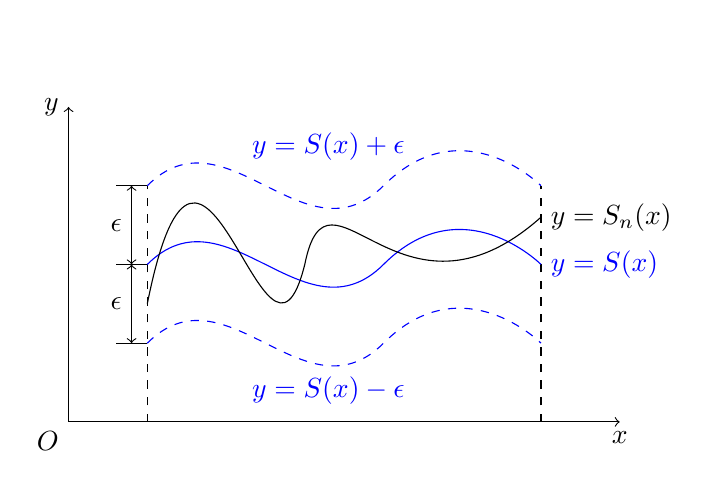
\begin{tikzpicture}
		\draw[->](0,0)node[below left]{\(O\)} -- (7,0)node[below]{\(x\)};
		\draw[->](0,0) -- (0,4)node[left]{\(y\)};
		\draw[dashed](1,0) -- (1,3) (6,0) -- (6,3);
		\draw(1,1)--+(-.4,0);
		\draw(1,2)--+(-.4,0);
		\draw(1,3)--+(-.4,0);
		\begin{scope}[<->,xshift=-.2cm]
			\draw(1,1) -- (1,2)node[midway,left]{\(\epsilon\)};
			\draw(1,2) -- (1,3)node[midway,left]{\(\epsilon\)};
		\end{scope}
		\begin{scope}[blue]
			\draw[dashed] (1,1) .. controls (2,2) and (3,0) .. (4,1) .. controls (5,2) and (6,1) .. (6,1);
			\draw[yshift=1cm] (1,1) .. controls (2,2) and (3,0) .. (4,1) .. controls (5,2) and (6,1) .. (6,1)node[right]{\(y = S(x)\)};
			\draw[yshift=2cm,dashed] (1,1) .. controls (2,2) and (3,0) .. (4,1) .. controls (5,2) and (6,1) .. (6,1);
			\draw(3.3,3.5)node{\(y = S(x) + \epsilon\)};
			\draw(3.3,0.4)node{\(y = S(x) - \epsilon\)};
		\end{scope}
		\draw(1,1.5) .. controls (1.7,5) and (2.5,0) .. (3,2) .. controls (3.3,3.5) and (4.2,1) .. (6,2.6)node[right]{\(y = S_n(x)\)};
	\end{tikzpicture}
	\caption{函数项级数一致收敛的几何解释}
	\label{figure:无穷级数.函数项级数一致收敛的几何解释}
\end{figure}

\begin{proposition}
%@see: 《数学分析(第二版 下册)》(陈纪修) P60 推论10.1.1
若函数项级数\(\sum_{n=1}^\infty u_n(x)\)在\(D\)上一致收敛,
则函数列\(\{u_n\}\)在\(D\)上一致收敛于\(u(x) \equiv 0\).
\begin{proof}
由\cref{definition:无穷级数.函数项级数的一致收敛性} 立即可得.
\end{proof}
\end{proposition}

\section{幂级数}
我们在本节学习函数项级数中简单而常见的一类函数项级数级数 --- “幂级数”.

\subsection{幂级数的概念}
\begin{definition}\label{definition:无穷级数.幂级数}
各项均是幂函数的函数项级数,
称为\DefineConcept{幂级数}(power series).

称级数\[
	\sum_{n=0}^\infty a_n (x-x_0)^n
\]为“幂级数的\DefineConcept{一般形式}”.

称级数\[
	\sum_{n=0}^\infty a_n x^n
\]为“幂级数的\DefineConcept{标准形式}”.

这里,我们把常数\(\AutoTuple{a}[0]{n},\dotsc\)称为
“幂级数的\DefineConcept{系数}”.
\end{definition}

由于幂级数的一般形式只要作变量代换\(t = x - x_0\)就可化为它的标准形式,
因此,即便我们取标准形式来讨论,也并不影响一般性.

\subsection{幂级数的收敛半径}
现在我们来讨论:
对于一个给定的幂级数,
它的收敛域与发散域是怎样的?
即\(x\)取数轴上哪些点时幂级数收敛,
取哪些点时幂级数发散?
这就是幂级数的收敛性问题.

先看一个例子.
考察幂级数\[
	1+x^2+x^3+\dotsb+x^n+\dotsb
\]的收敛性.
我们已经知道,
当\(\abs{x}<1\)时,
该级数收敛于\(\frac{1}{1-x}\);
当\(\abs{x}\geq1\)时,
该级数发散.
因此,这个幂级数的收敛域是开区间\((-1,1)\),
发散域是\((-\infty,-1]\cup[1,+\infty)\),
并有\[
	\frac{1}{1-x} = 1+x+x^2+\dotsb+x^n+\dotsb
	\quad(-1<x<1).
\]

在这个例子中我们看到,这个幂级数的收敛域是一个区间.
事实上,这个结论对于一般的幂级数也是成立的.
我们有如下的定理.

\begin{theorem}[阿贝尔第一定理]\label{theorem:无穷级数.阿贝尔定理1}
%@see: 《高等数学(第六版 下册)》 P271 定理1
%@see: 《数学分析(第二版 下册)》(陈纪修) P86 阿贝尔第一定理
如果级数\(\sum_{n=0}^\infty a_n x^n\)当\(x=x_0\neq0\)时收敛,
则满足\(\abs{x}<\abs{x_0}\)的一切\(x\)可使该幂级数绝对收敛.
反之,如果级数\(\sum_{n=0}^\infty a_n x^n\)当\(x=x_0\)时发散,
则满足\(\abs{x}>\abs{x_0}\)的一切\(x\)均使该幂级数发散.
\begin{proof}
先设\(x_0\)是幂级数\(\sum_{n=0}^\infty a_n x^n\)的收敛点,
即常数项级数\[
	a_0 + a_1 x_0 + a_2 x_0^2 + \dotsb + a_n x_0^n + \dotsb
\]收敛.
根据级数收敛的必要条件,
这时有\[
	\lim_{n\to\infty} a_n x_0^n = 0;
\]
于是\(\exists M > 0\),使得\[
	\abs{a_n x_0^n} \leq M
	\quad(n=0,1,2,\dotsc).
\]
这样幂级数\(\sum_{n=0}^\infty a_n x^n\)的一般项的绝对值\[
	\abs{a_n x^n} = \abs{a_n x_0^n \cdot \frac{x^n}{x_0^n}}
	= \abs{a_n x_0^n} \cdot \abs{\frac{x}{x_0}}^n
	\leq M \abs{\frac{x}{x_0}}^n.
\]
因为当\(\abs{x}<\abs{x_0}\)时,
等比级数\(\sum_{n=0}^\infty M \abs{\frac{x}{x_0}}^n\)收敛,
所以级数\(\sum_{n=1}^\infty \abs{a_n x^n}\)收敛,
也就是级数\(\sum_{n=0}^\infty a_n x^n\)绝对收敛.

定理的第二部分可用反证法证明.
假设幂级数当\(x=x_0\)时发散而有一点\(x_1\)适合\(\abs{x_1}>\abs{x_0}\)使级数收敛,
则根据本定理的第一部分,当\(x=x_0\)时级数应收敛,这与假设矛盾.
\end{proof}
\end{theorem}

\cref{theorem:无穷级数.阿贝尔定理1} 表明,
如果幂级数在\(x=x_0\)处收敛,
则对\(\forall x\in(-\abs{x_0},\abs{x_0})\),
幂级数都收敛;
如果幂级数在\(x=x_0\)处发散,
则对\(\forall x\in(-\infty,-\abs{x_0})\cup(\abs{x_0},+\infty)\),
幂级数都发散.

设已给幂级数在数轴上既有收敛点(不仅是原点)也有发散点.
现在从原点出发沿数轴正方向走,最初只遇到收敛点,然后就只遇到发散点.
这两部分的界点可能是收敛点,也可能是发散点.
从原点出发沿数轴负方向走,情形相同.
利用\cref{theorem:无穷级数.阿贝尔定理1} 可以证明:原点两侧的两个界点到原点的距离是相等的.
像这样,我们就得到以下重要推论.
\begin{corollary}\label{theorem:无穷级数.阿贝尔定理1推论}
%@see: 《高等数学(第六版 下册)》 P271 推论
%@see: 《数学分析(第二版 下册)》(陈纪修) P84 定理10.3.1(Cauchy-Hadamard定理)
如果幂级数\(\sum_{n=0}^\infty a_n x^n\)不是仅在\(x=0\)一点收敛,
也不是在整个数轴上都收敛,
则必定存在正数\(R\),
使得:\begin{itemize}
	\item 当\(\abs{x}<R\)时,幂级数绝对收敛;
	\item 当\(\abs{x}>R\)时,幂级数发散;
	\item 当\(\abs{x}=R\)时,幂级数可能收敛也可能发散.
\end{itemize}
%TODO proof
\end{corollary}

对于\(\sum_{n=0}^\infty a_n (x-x_0)^n\),我们有平行的结论:
如果幂级数\(\sum_{n=0}^\infty a_n (x-x_0)^n\)不是仅在\(x=x_0\)一点收敛,
也不是在整个数轴上都收敛,
则必定存在正数\(R\),
使得幂级数\(\sum_{n=0}^\infty a_n (x-x_0)^n\)
在以\(x_0\)为中心、以\(R\)为半径的对称区间\((x_0-R,x_0+R)\)内绝对收敛,
而在\((-\infty,x_0-R)\cup(x_0+R,+\infty)\)上发散.

我们把\cref{theorem:无穷级数.阿贝尔定理1推论} 中提到的正数\(R\)
称为“幂级数\(\sum_{n=0}^\infty a_n x^n\)的\DefineConcept{收敛半径}”.
把开区间\((-R,R)\)称为“幂级数\(\sum_{n=0}^\infty a_n x^n\)的\DefineConcept{收敛区间}”.

在已知幂级数的收敛半径或收敛区间的情况下,
我们可以根据幂级数在点\(x = \pm R\)处的收敛性,
就可以决定其收敛域是\((-R,R)\)、\([-R,R)\)、\((-R,R]\)或\([-R,R]\)四个区间之一.

如果幂级数只在\(x=0\)处收敛,这时收敛域为\(\{0\}\),规定收敛半径\(R=0\).
如果幂级数对任意实数都收敛,则规定收敛半径\(R=+\infty\),收敛域为\((-\infty,+\infty)\).

关于幂级数的收敛半径的求法,有下面的定理.
\begin{theorem}\label{theorem:无穷级数.幂级数的收敛半径的求法1}
%@see: 《数学分析(第二版 下册)》(陈纪修) P84
如果\[
	\varlimsup_{n\to\infty} \sqrt[n]{\abs{a_n}} = \rho,
\]
则幂级数\(\sum_{n=0}^\infty a_n x^n\)的收敛半径为\[
	R = \left\{ \def\arraystretch{1.5} \begin{array}{cl}
		\frac1\rho, & 0<\rho<+\infty, \\
		+\infty, & \rho = 0, \\
		0, & \rho = +\infty \\
	\end{array} \right.
\]
\end{theorem}
\begin{remark}
从\cref{theorem:无穷级数.幂级数的收敛半径的求法1} 可以看出:
给定两个幂级数\(\sum_{n=0}^\infty a_n x^n\)和\(\sum_{n=0}^\infty b_n x^n\),
假设它们的收敛半径分别是\(R_1\)和\(R_2\),
如果\(\abs{a_n} \leq \abs{b_n}\ (n=1,2,\dotsc)\),
那么必有\(\sqrt[n]{\abs{a_n}} \leq \sqrt[n]{\abs{b_n}}\),
从而有\(R_1 \geq R_2\).
\end{remark}

\begin{example}
%@see: 《数学分析(第二版 下册)》(陈纪修) P85 例10.3.2
考察幂级数\(\sum_{n=1}^\infty \frac{[2+(-1)^n]^n}{n} \left(x-\frac12\right)^n\)的敛散性.
\begin{solution}
因为\[
	\varlimsup_{n\to\infty} \sqrt[n]{\frac{[2+(-1)^n]^n}n} = 3,
\]
所以收敛半径为\(R=\frac13\).
当\(x=\frac12+R=\frac56\)时,
级数\(\sum_{n=1}^\infty \frac{[2+(-1)^n]^n}{3^n n}\)是发散的.
当\(x=\frac12-R=\frac16\)时,
级数\(\sum_{n=1}^\infty \frac{[2+(-1)^n]^n}{6^n n}\)是发散的.
因此幂级数\(\sum_{n=1}^\infty \frac{[2+(-1)^n]^n}{n} \left(x-\frac12\right)^n\)的收敛域是
\(\left(\frac16,\frac56\right)\).
\end{solution}
\end{example}

\begin{theorem}\label{theorem:无穷级数.幂级数的收敛半径的求法2}
%@see: 《高等数学(第六版 下册)》 P272 定理2
%@see: 《数学分析(第二版 下册)》(陈纪修) P85 定理10.3.2(d'Alembert判别法)
如果\[
	\lim_{n\to\infty} \abs{\frac{a_{n+1}}{a_n}} = \rho,
\]
则幂级数\(\sum_{n=0}^\infty a_n x^n\)的收敛半径为\[
	R = \left\{ \def\arraystretch{1.5} \begin{array}{cl}
		\frac1\rho, & 0<\rho<+\infty, \\
		+\infty, & \rho = 0, \\
		0, & \rho = +\infty. \\
	\end{array} \right.
\]
\begin{proof}
考察幂级数\(\sum_{n=0}^\infty a_n x^n\)的各项取绝对值所成的级数\[
	\sum_{n=1}^\infty \abs{a_n x^n}
	= \abs{a_0} + \abs{a_1 x} + \abs{a_2 x^2} + \dotsb + \abs{a_n x^n} + \dotsb.
\]
这级数相邻两项之比为\[
	\frac{\abs{a_{n+1} x^{n+1}}}{\abs{a_n x^n}}
	= \abs{\frac{a_{n+1}}{a_n}} \abs{x}.
\]

\begin{enumerate}
	\item 如果极限\(\lim_{n\to\infty} \abs{\frac{a_{n+1}}{a_n}} = \rho\neq0\)存在,
	根据\hyperref[theorem:无穷级数.正项级数的比值审敛法]{比值审敛法},
	则当\(\rho \abs{x} < 1\)即\(\abs{x} < \frac1\rho\)时,
	级数\(\sum_{n=1}^\infty \abs{a_n x^n}\)收敛,
	从而级数\(\sum_{n=0}^\infty a_n x^n\)绝对收敛;
	再根据\cref{theorem:无穷级数.绝对发散的特殊情况},
	当\(\rho \abs{x} > 1\)即\(\abs{x} > \frac1\rho\)时,
	级数\(\sum_{n=1}^\infty \abs{a_n x^n}\)发散,
	并且\[
		(\exists N\in\mathbb{N})
		(\forall n\in\mathbb{N})
		[
			n > N
			\implies
			\abs{a_{n+1} x^{n+1}} > \abs{a_n x^n}
		].
	\]

	\item 如果\(\rho=0\),
	则对\(\forall x\neq0\),
	有\(\lim_{n\to\infty} \abs{\frac{a_{n+1} x^{n+1}}{a_n x^n}} = 0\),
	所以级数\(\sum_{n=1}^\infty \abs{a_n x^n}\)收敛,
	从而级数\(\sum_{n=0}^\infty a_n x^n\)绝对收敛.
	于是\(R=+\infty\).
		\item 如果\(\rho=+\infty\),
	则对\(\forall x\neq0\),
	级数\(\sum_{n=0}^\infty a_n x^n\)必发散,
	否则由\cref{theorem:无穷级数.阿贝尔定理1} 知道,
	\(\exists x\neq0\)使得\(\sum_{n=1}^\infty \abs{a_n x^n}\)收敛.
	于是\(R=0\).
	\qedhere
\end{enumerate}
\end{proof}
\end{theorem}
\begin{remark}
当级数缺项(即某些项取值为零)时,
不能直接运用\cref{theorem:无穷级数.幂级数的收敛半径的求法2} 求解幂级数的收敛半径,
可以把\(x\)看成常数,把\(\sum_{n=0}^\infty a_n x^n\)看成常数项级数,
使用合适的审敛法(例如\hyperref[theorem:无穷级数.正项级数的比值审敛法]{比值审敛法},
或\hyperref[theorem:无穷级数.正项级数的根值审敛法]{根值审敛法}),
或者对幂级数使用换元法.
\end{remark}

\begin{example}
%@see: 《数学分析(第二版 下册)》(陈纪修) P86 例10.3.3
考察幂级数\(\sum_{n=0}^\infty \frac{n^n}{n!} x^n\)的收敛情况.
\begin{solution}
因为\[
	\lim_{n\to\infty} \abs{\frac{a_{n+1}}{a_n}}
	= \lim_{n\to\infty} \frac{(n+1)^{n+1} / (n+1)!}{n^n / n!}
	= e,
\]
所以收敛半径为\(R=1/e\).

当\(x=1/e\)时,
\(\sum_{n=0}^\infty \frac{n^n}{n!} x^n\)是正项级数,
由\hyperref[example:无穷乘积.斯特林公式]{斯特林公式}
\(n! \sim \sqrt{2\pi n} (n/e)^n\ (n\to\infty)\)有\[
	\frac{n^n}{n!} x^n
	\sim
	\frac{n^n}{\sqrt{2\pi} n^{n+1/2} e^{-n}} \cdot \frac1{e^n}
	= \frac1{\sqrt{2\pi n}}
	\quad(n\to\infty),
\]
可知\(\sum_{n=0}^\infty \frac{n^n}{n!} x^n\)在点\(x=1/e\)发散.

当\(x=-1/e\)时,
\(\sum_{n=0}^\infty \frac{n^n}{n!} x^n\)是交错级数,
由于\[
	\abs{\frac{(n+1)^{n+1} x^{n+1} / (n+1)!}{n^n x^n / n!}}
	= \frac1e \left( 1 + \frac1n \right)^n
	< 1,
\]
且\[
	\abs{\frac{n^n}{n!} x^n}
	\sim
	\frac1{\sqrt{2\pi n}}
	\to 0
	\quad(n\to\infty),
\]
可知\(\sum_{n=0}^\infty \frac{n^n}{n!} x^n\)
在点\(x=-1/e\)成为莱布尼茨级数,必定收敛.

综上所述,
\(\sum_{n=0}^\infty \frac{n^n}{n!} x^n\)的收敛域是\([-1/e,1/e)\).
\end{solution}
\end{example}

\begin{example}
%@see: 《高等数学(第六版 下册)》 P273 例1
求幂级数\[
	x-\frac{x^2}{2}+\frac{x^3}{3}-\dotsb+(-1)^{n-1}\frac{x^n}{n}+\dotsb
\]的收敛半径与收敛域.
\begin{solution}
因为\[
	\rho = \lim_{n\to\infty} \abs{\frac{a_{n+1}}{a_n}}
	= \lim_{n\to\infty} \frac{n}{n+1} = 1,
\]
所以收敛半径\[
	R = \frac1\rho = 1.
\]

对于端点\(x=1\),级数成为交错级数\[
	1-\frac{1}{2}+\frac{1}{3}-\dotsb+(-1)^{n-1}\frac{1}{n}+\dotsb,
\]
由\cref{example:无穷级数.交错级数1} 可知,此级数收敛;
对于端点\(x=-1\),级数成为\[
	-1-\frac{1}{2}-\frac{1}{3}-\dotsb-\frac{1}{n}-\dotsb,
\]
此级数发散.
综上所述,收敛域是\((-1,1]\).
\end{solution}
\end{example}
利用上例的结果可以计算出交错级数\[
	1-\frac{1}{2}+\frac{1}{3}-\dotsb+(-1)^{n-1}\frac{1}{n}+\dotsb.
\]
显然有\begin{align*}
	\sum_{n=1}^\infty (-1)^{n-1} \frac{1}{n}
	&= \eval{\sum_{n=1}^\infty (-1)^{n-1} \frac{x^n}{n}}_{x=1} \\
	&= \eval{\sum_{n=1}^\infty (-1)^{n-1} \int_0^x \left(\frac{x^n}{n}\right)' \dd{x}}_{x=1} \\
	&= \eval{\sum_{n=1}^\infty (-1)^{n-1} \int_0^x x^{n-1} \dd{x}}_{x=1} \\
	&= \eval{\int_0^x \sum_{n=1}^\infty (-1)^{n-1} x^{n-1} \dd{x}}_{x=1} \\
	&= \eval{\int_0^x \frac{1}{1+x} \dd{x}}_{x=1} \\
	&= \eval{\ln(1+x)}_{x=1} = \ln2.
\end{align*}
\begin{example}
%@see: 《2009年全国硕士研究生入学统一考试(数学一)》三解答题/第16题
设\(a_n\)是曲线\(y=x^n\)与\(y=x^{n+1}\)所围成区域的面积,
计算级数\(\sum_{n=1}^\infty a_{2n-1}\).
\begin{solution}
因为\(y = x^n\)与\(y = x^{n+1}\)只交于\((0,0)\)和\((1,1)\)两点,
且当\(0 < x < 1\)时总有\(x^n > x^{n+1}\),
所以\[
	a_n = \int_0^1 (x^n - x^{n+1}) \dd{x}
	= \frac1{n+1} - \frac1{n+2},
\]
于是\[
	\sum_{n=1}^\infty a_{2n-1}
	= \frac12 - \frac13 + \frac14 - \frac15 + \dotsb.
\]
而\[
	1 - \left(\frac12 - \frac13 + \frac14 - \frac15 + \dotsb\right)
	= \ln2,
\]
因此\(\sum_{n=1}^\infty a_{2n-1} = 1 - \ln2\).
\end{solution}
\end{example}

\begin{example}
%@see: 《高等数学(第六版 下册)》 P273 例2
求幂级数\[
	1+x+\frac{1}{2!}x^2+\dotsb+\frac{1}{n!}x^n+\dotsb
\]的收敛域.
\begin{solution}
因为\[
	\rho = \lim_{n\to\infty} \abs{\frac{a_{n+1}}{a_n}}
	= \lim_{n\to\infty} \frac{n!}{(n+1)!}
	= \lim_{n\to\infty} \frac{1}{n+1}
	= 0,
\]
所以收敛半径\(R = +\infty\),从而收敛域是\((-\infty,+\infty)\).
\end{solution}
\end{example}

\begin{example}
%@see: 《高等数学(第六版 下册)》 P273 例3
求幂级数\(\sum_{n=0}^\infty n! x^n\)的收敛半径.
\begin{solution}
因为\[
	\rho
	= \lim_{n\to\infty} \abs{\frac{a_{n+1}}{a_n}}
	= \lim_{n\to\infty} \frac{(n+1)!}{n!}
	= \lim_{n\to\infty} (n+1)
	= +\infty,
\]
所以收敛半径\(R = 0\),
即级数仅在点\(x = 0\)处收敛.
\end{solution}
\end{example}

\begin{example}
%@see: 《高等数学(第六版 下册)》 P274 例4
求幂级数\(\sum_{n=0}^\infty \frac{(2n)!}{(n!)^2} x^{2n}\)的收敛半径.
\begin{solution}
级数缺少奇次幂的项,\cref{theorem:无穷级数.幂级数的收敛半径的求法2} 不能直接应用,
我们根据\cref{theorem:无穷级数.正项级数的比值审敛法的上下极限形式} 来求收敛半径:
\[
	\lim_{n\to\infty} \abs{
		{\frac{[2(n+1)]!}{[(n+1)!]^2} x^{2(n+1)}}
		\Bigg/
		{\frac{(2n)!}{(n!)^2} x^{2n}}
	}
	= \lim_{n\to\infty} \abs{\frac{(2n+2)(2n+1)}{(n+1)^2} x^2}
	= 4 x^2.
\]

当\(4 x^2 < 1\)即\(\abs{x} < 1/2\)时级数收敛;
当\(4 x^2 > 1\)即\(\abs{x} > 1/2\)时级数发散.
所以收敛半径\(R = 1/2\).
\end{solution}
\end{example}

\begin{example}
%@see: 《高等数学(第六版 下册)》 P274 例4
求幂级数\(\sum_{n=1}^\infty \frac{(x-1)^n}{2^n \cdot n}\)的收敛域.
\begin{solution}
令\(t = x-1\),上述级数变为\[
	\sum_{n=1}^\infty \frac{t^n}{2^n \cdot n}.
\]
因为\[
	\rho
	= \lim_{n\to\infty} \abs{\frac{a_{n+1}}{a_n}}
	= \lim_{n\to\infty} \frac{2^n \cdot n}{2^{n+1} \cdot (n+1)}
	= \frac{1}{2},
\]
所以收敛半径\(R_t = 2\),而原级数的收敛区间为\(-1<x<3\).

当\(x=3\)时,级数成为\(\sum_{n=1}^\infty \frac{1}{n}\),这级数发散;
当\(x=-1\)时,级数成为\(\sum_{n=1}^\infty \frac{(-1)^n}{n}\),这级数收敛.
因此原级数的收敛域为\([-1,3)\).
\end{solution}
\end{example}

\begin{example}
%@see: 《数学分析(第二版 下册)》(陈纪修) P94 习题 8.
设正项级数\(\sum_{n=1}^\infty a_n\)发散,
\(A_n = \sum_{k=1}^n a_k\),
且\(\lim_{n\to\infty} \frac{a_n}{A_n} = 0\).
求幂级数\(\sum_{n=1}^\infty a_n x^n\)的收敛半径.
\begin{solution}
设\(\sum_{n=1}^\infty a_n x^n\)的收敛半径为\(R_1\),
\(\sum_{n=1}^\infty A_n x^n\)的收敛半径为\(R_2\).

由于\(a_n\geq0\ (n=1,2,\dotsc)\),
所以\(a_n \leq A_n\),
从而有\(R_1 \geq R_2\).

又因为\(\sum_{n=1}^\infty a_n\)发散,
由\cref{theorem:无穷级数.正项级数的比值审敛法} 可知
\(\lim_{n\to\infty} \frac{a_{n+1}}{a_n} \geq 1\),
所以\(R_1 \leq 1\).

由于\[
	\lim_{n\to\infty} \frac{A_n}{A_{n+1}}
	= \lim_{n\to\infty} \frac{A_{n+1} - a_{n+1}}{A_{n+1}}
	= 1,
\]
所以\(R_2=1\).

综上所述,既然\(1 \leq R_1 \leq 1\),则必有\(R_1=1\).
\end{solution}
\end{example}

\subsection{幂级数的性质}
\begin{theorem}[阿贝尔第二定理]\label{theorem:无穷级数.阿贝尔定理2}
%@see: 《数学分析(第二版 下册)》(陈纪修) P87 定理10.3.3(Abel第二定理)
设幂级数\(\sum_{n=0}^\infty a_n x^n\)的收敛半径为\(R\),
则\begin{itemize}
	\item \(\sum_{n=0}^\infty a_n x^n\)在\((-R,R)\)上内闭一致收敛;
	\item \(\sum_{n=0}^\infty a_n x^n\)在包含于它的收敛域的任意闭区间上一致收敛,
	即\begin{itemize}
		\item 若\(\sum_{n=0}^\infty a_n x^n\)在点\(x=R\)收敛,
		则它在任意闭区间\([a,R]\subseteq(-R,R]\)上一致收敛;
		\item 若\(\sum_{n=0}^\infty a_n x^n\)在点\(x=-R\)收敛,
		则它在任意闭区间\([-R,b]\subseteq[-R,R)\)上一致收敛;
		\item 若\(\sum_{n=0}^\infty a_n x^n\)在点\(x=\pm R\)都收敛,
		则它在闭区间\([-R,R]\)上一致收敛.
	\end{itemize}
\end{itemize}
%TODO proof
\end{theorem}

根据\hyperref[theorem:无穷级数.阿贝尔定理2]{阿贝尔第二定理},
我们可以得到幂级数的如下几个性质.

\begin{property}\label{theorem:无穷级数.幂级数的和函数的性质1}
%@see: 《数学分析(第二版 下册)》(陈纪修) P87 定理10.3.4
%@see: 《高等数学(第六版 下册)》 P276 性质1
幂级数\(\sum_{n=0}^\infty a_n x^n\)的和函数在其收敛域上连续.
\begin{proof}
幂级数的一般项是幂函数,显然是连续函数.
由\hyperref[theorem:无穷级数.阿贝尔定理2]{阿贝尔第二定理},
\(\sum_{n=0}^\infty a_n x^n\)在其收敛域上内闭一致收敛.
根据\hyperref[theorem:函数项级数.连续函数项级数的内闭一致收敛性保证和函数的连续性]{一致收敛函数项级数的和函数的连续性},
\(\sum_{n=0}^\infty a_n x^n\)在包含于收敛域中的任意闭区间上连续,
因而在它的整个收敛域上连续.
\end{proof}
\end{property}

\begin{property}\label{theorem:无穷级数.幂级数的和函数的性质2}
%@see: 《数学分析(第二版 下册)》(陈纪修) P87 定理10.3.4
%@see: 《高等数学(第六版 下册)》 P276 性质2
幂级数\(\sum_{n=0}^\infty a_n x^n\)
在包含于其收敛域中的任意闭区间上
可以逐项求积分,
即对于其收敛域内的任意两点\(a,b\),
有\begin{equation}
	\int_a^b \sum_{n=0}^\infty a_n x^n \dd{x}
	= \sum_{n=0}^\infty \int_a^b a_n x^n \dd{x}.
\end{equation}
特别地,有\begin{equation}
	\int_0^x \sum_{n=0}^\infty a_n t^n \dd{t}
	= \sum_{n=0}^\infty \frac{a_n}{n+1} x^{n+1},
\end{equation}
且逐项积分所得到的幂级数\(\sum_{n=0}^\infty \frac{a_n}{n+1} x^{n+1}\)
和原幂级数\(\sum_{n=0}^\infty a_n x^n\)
具有相同的收敛半径.
\begin{proof}
由\hyperref[theorem:无穷级数.阿贝尔定理2]{阿贝尔第二定理},
\(\sum_{n=0}^\infty a_n x^n\)在其收敛域上内闭一致收敛.
应用\hyperref[theorem:函数项级数.连续函数项级数的一致收敛性保证和函数的可积性]{一致收敛函数项级数的逐项积分定理},
就得到幂级数的逐项可积性.

由于\[
	\varlimsup_{n\to\infty} \sqrt[n+1]{\frac{\abs{a_n}}{n+1}}
	= \varlimsup_{n\to\infty} \sqrt[n]{\abs{a_n}},
\]
所以\(\sum_{n=0}^\infty \frac{a_n}{n+1} x^{n+1}\)
与\(\sum_{n=0}^\infty a_n x^n\)具有相同的收敛半径.
\end{proof}
\end{property}
\begin{remark}
虽然逐项积分所得的幂级数\(\sum_{n=0}^\infty \frac{a_n}{n+1} x^{n+1}\)
和原幂级数\(\sum_{n=0}^\infty a_n x^n\)收敛半径相同,
但是它的收敛域相比于原幂级数可能扩大.

%@see: 《数学分析(第二版 下册)》(陈纪修) P89 例10.3.4
例如,幂级数\[
	\sum_{n=1}^\infty (-1)^{n-1} x^{2n-2}
\]的收敛域是\((-1,1)\),
但逐项积分所得的幂级数\[
	\sum_{n=1}^\infty \frac{(-1)^{n-1}}{2n-1} x^{2n-1}
\]的收敛域是\([-1,1]\).

%@see: 《数学分析(第二版 下册)》(陈纪修) P89 例10.3.5
又例如,幂级数\[
	\sum_{n=1}^\infty (-1)^{n-1} x^{n-1}
\]的收敛域是\((-1,1)\),
但逐项积分所得的幂级数\[
	\sum_{n=1}^\infty \frac{(-1)^{n-1}}{n} x^n
\]的收敛域是\((-1,1]\).
\end{remark}

\begin{property}\label{theorem:无穷级数.幂级数的和函数的性质3}
%@see: 《数学分析(第二版 下册)》(陈纪修) P89 定理10.3.6
%@see: 《高等数学(第六版 下册)》 P276 性质3
幂级数\(\sum_{n=0}^\infty a_n x^n\)
在其收敛区间上可以逐项求导,
即\begin{equation}
	\dv{x} \sum_{n=0}^\infty a_n x^n
	= \sum_{n=0}^\infty \dv{x} a_n x^n
	= \sum_{n=1}^\infty n a_n x^{n-1}
	\quad(-R<x<R),
\end{equation}
其中\(R\)是\(\sum_{n=0}^\infty a_n x^n\)的收敛半径,
且逐项求导所得的幂级数\(\sum_{n=1}^\infty n a_n x^{n-1}\)的收敛半径也是\(R\).
\end{property}
\begin{remark}
虽然逐项积分所得的幂级数\(\sum_{n=1}^\infty n a_n x^{n-1}\)
和原幂级数\(\sum_{n=0}^\infty a_n x^n\)收敛半径相同,
但是它的收敛域相比于原幂级数可能缩小.

例如,幂级数\[
	\sum_{n=1}^\infty \frac{(-1)^{n-1}}{2n-1} x^{2n-1}
\]的收敛域是\([-1,1]\),
但逐项求导所得的幂级数\[
	\sum_{n=1}^\infty (-1)^{n-1} x^{2n-2}
\]的收敛域是\((-1,1)\).
\end{remark}

反复利用\cref{theorem:无穷级数.幂级数的和函数的性质3} 可得以下结论.
\begin{proposition}
幂级数\(\sum_{n=0}^\infty a_n x^n\)的和函数
在其收敛区间\((-R,R)\)内具有任意阶导数.
\end{proposition}

\begin{example}
求幂级数\(\sum_{n=1}^\infty \frac{x^n}{n+1}\)的和函数.
\begin{solution}
先求收敛域.
由\[
	\lim_{n\to\infty} \abs{\frac{a_{n+1}}{a_n}}
	= \lim_{n\to\infty} \frac{n+1}{n+2}
	= 1,
\]
得收敛半径\(R=1\).

在端点\(x = -1\)处,
幂级数成为\(\sum_{n=1}^\infty \frac{(-1)^n}{n+1}\),
是收敛的交错级数;
在端点\(x = 1\)处,
幂级数成为\(\sum_{n=1}^\infty \frac{1}{n+1}\),
是发散的.
因此收敛域是\(I = [-1,1)\).

设和函数为\(s(x)\),即\[
	s(x) = \sum_{n=1}^\infty \frac{x^n}{n+1},
	\quad x\in[-1,1).
\]
于是\[
	x s(x) = \sum_{n=1}^\infty \frac{x^{n+1}}{n+1}.
\]

利用\cref{theorem:无穷级数.幂级数的和函数的性质3},逐项求导,并由\[
	\frac{1}{1-x} = 1+x+x^2+\dotsb+x^n+\dotsb
	\quad(-1<x<1),
\]
得\[
	[x s(x)]'
	= \sum_{n=1}^\infty \left( \frac{x^{n+1}}{n+1} \right)'
	= \sum_{n=1}^\infty x^n
	= \frac{1}{1-x}
	\quad(\abs{x}<1).
\]
对上式积分,
得\[
	x s(x) = \int_0^x \frac{1}{1-x} \dd{x} = -\ln(1-x)
	\quad(-1 \leq x < 1).
\]
于是,当\(x\neq0\)时,有\(s(x) = -\frac{1}{x} \ln(1-x)\).

而\(s(0)\)可由\(s(0) = a_0 = 1\)得出,
或者由和函数的连续性得到,即\[
	s(0)
	= \lim_{x\to0} s(x)
	= \lim_{x\to0} \left[ -\frac{1}{x} \ln(1-x) \right]
	= 1.
\]
故\[
	s(x) = \left\{ \begin{array}{cl}
		-\frac{1}{x} \ln(1-x), & x\in[-1,0)\cup(0,1), \\
		1, & x=0.
	\end{array} \right.
\]
\end{solution}
\end{example}





\subsection{幂级数的运算}
\begin{definition}
设幂级数\(\sum_{n=0}^\infty a_n x^n\)
和\(\sum_{n=0}^\infty b_n x^n\)
分别在区间\((-R,R)\)和\((-R',R')\)内收敛.
定义:
\begin{gather}
	\left(\sum_{n=0}^\infty a_n x^n\right)
	+ \left(\sum_{n=0}^\infty b_n x^n\right)
	\defeq
	\sum_{n=0}^\infty (a_n+b_n) x^n, \\
	\left(\sum_{n=0}^\infty a_n x^n\right)
	- \left(\sum_{n=0}^\infty b_n x^n\right)
	\defeq
	\sum_{n=0}^\infty (a_n-b_n) x^n, \\
	\left(\sum_{n=0}^\infty a_n x^n\right)
	\cdot \left(\sum_{n=0}^\infty b_n x^n\right)
	\defeq
	\sum_{n=0}^\infty \left(
		\sum_{i=0}^n a_i b_{n-i}
	\right) x^n.
\end{gather}
\end{definition}

\begin{definition}
设幂级数\(\sum_{n=0}^\infty a_n x^n\)
和\(\sum_{n=0}^\infty b_n x^n\)
分别在区间\((-R,R)\)和\((-R',R')\)内收敛.

记\[
	\frac{
		\sum_{n=0}^\infty a_n x^n
	}{
		\sum_{n=0}^\infty b_n x^n
	}
	= \sum_{n=0}^\infty c_n x^n,
\]
假设\(b_0 \neq 0\).
为了决定系数\(c_0,c_1,\dotsc,c_n,\dotsc\),
可以将级数\(\sum_{n=0}^\infty b_n x^n\)
与\(\sum_{n=0}^\infty c_n x^n\)相乘,
并令乘积中各项的系数分别等于级数\(\sum_{n=0}^\infty a_n x^n\)中同次幂的系数,
即得\[
	\begin{cases}
		a_0 = b_0 c_0, \\
		a_1 = b_1 c_0 + b_0 c_1, \\
		a_2 = b_2 c_0 + b_1 c_1 + b_0 c_2, \\
		\hdotsfor{1} \\
	\end{cases}
\]
由这些方程就可以顺序地求出\(c_0,c_1,\dotsc,c_n,\dotsc\).

相除后所得的幂级数\(\sum_{n=0}^\infty c_n x^n\)的收敛区间可能比原来的两级数的收敛区间小得多.
\end{definition}

例如,级数\[
	\sum_{n=0}^\infty a_n x^n
	= 1 + 0x + \dotsb + 0x^n + \dotsb
\]与\[
	\sum_{n=0}^\infty b_n x^n
	= 1 - x + 0x^2 + \dotsb + 0x^n + \dotsb
\]在整个数轴上收敛,
但是这两个级数的商\(\sum_{n=0}^\infty c_n x^n
= \sum_{n=0}^\infty x^n\)仅在区间\((-1,1)\)内收敛.

\section{函数展开成幂级数}
前面讨论了幂级数的收敛域及其和函数的性质.
但在许多应用中,我们遇到的却是相反的问题:
给定函数\(f(x)\),
要考虑它是否能在某个区间内“展开成幂级数”,
就是说,是否能找到这样一个幂级数,它在某区间内收敛,且其和恰好就是给定的函数\(f(x)\).
如果能找到这样的幂级数,我们就说“函数\(f(x)\)在该区间内能展开成幂级数”,
也说“这个幂级数在该区间内表达了函数\(f(x)\)”.

\subsection{泰勒展式}
\begin{definition}
设函数\(f\colon D\to\mathbb{R}\).
如果在区间\(I \subseteq D\)内,
存在收敛的幂级数\(\sum_{n=0}^\infty a_n x^n\)使得\[
	f(x) = \sum_{n=0}^\infty a_n x^n
	\quad(x \in I)
\]成立,
则称“函数\(f(x)\)在区间\(I\)内能展开成幂级数”.
\end{definition}

\begin{definition}
级数\[
	\sum_{n=0}^\infty \frac{1}{n!} f^{(n)}(x_0) (x-x_0)^n
\]
为“函数\(f(x)\)在点\(x_0\)处的\DefineConcept{泰勒级数}(Taylor series)”.
%@see: https://mathworld.wolfram.com/TaylorSeries.html

等式\[
	f(x) = \sum_{n=0}^\infty {\frac{1}{n!} f^{(n)}(x_0) (x-x_0)^n},
	\quad x \in U(x_0).
\]
称为“函数\(f(x)\)在点\(x_0\)处的\DefineConcept{泰勒展开式}”.
\end{definition}

可以看出,函数\(f(x)\)在\(U(x_0)\)内能展开成幂级数的充分必要条件为:
泰勒级数\[
	\sum_{n=0}^\infty {\frac{1}{n!} f^{(n)}(x_0) (x-x_0)^n}
\]在\(U(x_0)\)内收敛,
且收敛到\(f(x)\).
但是“泰勒级数收敛到函数\(f(x)\)”这一叙述非常模糊,所以我们有以下定理:
\begin{theorem}
设函数\(f(x)\)在点\(x_0\)的某一邻域\(U(x_0)\)内具有各阶导数,
则\(f(x)\)在该邻域内能展开成泰勒级数的充分必要条件是:
在该邻域内\(f(x)\)的泰勒公式中的余项\(R_n(x)\)满足\[
	\lim_{n\to\infty} R_n(x) = 0,
	\quad x \in U(x_0).
\]
\end{theorem}

\begin{definition}
级数\[
	\sum_{n=0}^\infty \frac{1}{n!} f^{(n)}(0) x^n
\]
称为函数\(f(x)\)的\DefineConcept{麦克劳林级数}.

等式\[
	f(x) = \sum_{n=0}^\infty {\frac{1}{n!} f^{(n)}(0) x^n}
	\quad(\abs{x} < r)
\]
称为函数\(f(x)\)的\DefineConcept{麦克劳林展开式}.
\end{definition}

\begin{theorem}
若函数\(f(x)\)在区间\(I\)内能展开成幂级数,
则它的幂级数展开式是唯一的.
\end{theorem}

{\color{red}
要把函数\(f(x)\)展开成麦克劳林级数,可以按照下列步骤进行:
\begin{enumerate}
\item 求出函数\(f(x)\)的各阶导数\[
f'(x),f''(x),\dotsc,f^{(n)}(x),\dotsc.
\]如果在\(x=0\)处某阶导数不存在,就停止展开,因为这就说明函数\(f(x)\)不能展开为麦克劳林级数.
\item 求出函数及其各阶导数在\(x=0\)处的值:\[
f(0),f'(0),f''(0),\dotsc,f^{(n)}(0),\dotsc.
\]
\item 写出幂级数\[
f(0) + f'(0) x + \frac{f''(0)}{2!} x^2 + \dotsb + \frac{f^{(n)}(0)}{n!} x^n + \dotsb,
\]并求出收敛半径\(R\).
\item 利用余项\(R_n(x)\)的表达式\[
R_n(x) = \frac{1}{(n+1)!} f^{(n+1)}(\theta x) x^{n+1}
\quad(0 < \theta < 1),
\]考察当\(x\)在区间\((-R,R)\)内时余项的极限\(\lim_{n\to\infty} R_n(x)\)是否为零.

如果\(\lim_{n\to\infty} R_n(x) = 0\),则函数\(f(x)\)在区间\((-R,R)\)内的麦克劳林展开式为\[
f(x) = \sum_{n=0}^\infty \frac{1}{n!} f^{(n)}(0) x^n
\quad(-R < x < R).
\]

如果\(\lim_{n\to\infty} R_n(x) \neq 0\),则函数\(f(x)\)不能展开为麦克劳林级数.
\end{enumerate}
}

需要注意的是,不要错误地认为“如果一个函数的泰勒级数在点\(x_0\)处收敛,那么该级数就一定收敛到这个函数”.
\begin{example}\label{example:无穷级数.函数的泰勒级数不一定收敛到函数}
最常见的例子是:\[
f(x) = \left\{ \begin{array}{ll}
e^{-1/x^2}, & x\neq0, \\
0, & x=0.
\end{array} \right.
\]
根据导数的定义,以及\(\forall k\in\mathbb{R}: x^k e^{-1/x^2} \to 0\ (x\to0)\),
可知\(f^{(n)}(0) = 0\ (n=0,1,2,\dotsc)\).
于是,函数\(f\)在点\(x=0\)处的泰勒级数的每一项都是零,其和恒等于零;
只不过,当\(x\neq0\)时,\(f(x)\neq0\).
\end{example}

\begin{example}
将函数\(f(x) = e^x\)展开成\(x\)的幂级数.
\begin{solution}
所给函数的各阶导数为\[
f^{(n)}(x) = e^x
\quad(n=1,2,\dotsc),
\]因此\[
f^{(n)}(x) = 1
\quad(n=0,1,2,\dotsc).
\]于是得级数\[
1+x+\frac{x^2}{2!}+\dotsb+\frac{x^n}{n!}+\dotsb,
\]它的收敛半径\(R = +\infty\).

对于任何有限的数\(x\)和\(\xi\)(\(\xi\)在\(0\)与\(x\)之间),余项的绝对值为\[
\abs{R_n(x)} = \abs{\frac{e^{\xi}}{(n+1)!} x^{n+1}}
< e^{\abs{x}} \cdot \frac{\abs{x}^{n+1}}{(n+1)!}.
\]因为\(e^{\abs{x}}\)有限,而\(\frac{\abs{x}^{n+1}}{(n+1)!}\)是收敛级数\(\sum_{n=0}^\infty \frac{\abs{x}^{n+1}}{(n+1)!}\)的一般项,所以当\(n\to\infty\)时,\(e^{\abs{x}} \cdot \frac{\abs{x}^{n+1}}{(n+1)!}\to0\),即\[
\lim_{n\to\infty} \abs{R_n(x)} = 0.
\]于是得展开式\[
e^x = 1+x+\frac{x^2}{2!}+\dotsb+\frac{x^n}{n!}+\dotsb
\quad(-\infty<x<+\infty).
\]
\end{solution}
\end{example}

\begin{example}
将函数\(f(x) = \sin x\)展开成\(x\)的幂级数.
\begin{solution}
所给函数的各阶导数为\[
f^{(n)}(x) = \sin\left(x + n\cdot\frac{\pi}{2}\right)
\quad(n=1,2,\dotsc),
\]易见\(f^{(n)}(0)\)依顺序循环地取\(0,1,0,-1,\dotsc\),于是得级数\[
x-\frac{x^3}{3!}+\frac{x^5}{5!}-\dotsb+(-1)^k \frac{x^{2k+1}}{(2k+1)!}+\dotsb,
\]它的收敛半径\(R=+\infty\).

对于任何有限的数\(x\)和\(\xi\)(\(\xi\)在\(0\)与\(x\)之间),余项的绝对值为\[
\abs{R_n(x)}
= \abs{ \frac{x^{n+1}}{(n+1)!} \sin\left[\xi+\frac{n+1}{2}\pi\right] }
\leq \frac{\abs{x}^{n+1}}{(n+1)!}.
\]而\[
\lim_{n\to\infty} \frac{\abs{x}^{n+1}}{(n+1)!} = 0.
\]因而得展开式\[
\sin x = x-\frac{x^3}{3!}+\frac{x^5}{5!}-\dotsb+(-1)^k \frac{x^{2k+1}}{(2k+1)!}+\dotsb
\quad(-\infty<x<+\infty).
\]
\end{solution}
\end{example}

以上将函数展开成幂级数的例子,是直接按公式\[
a_n = \frac{1}{n!} f^{(n)}(0)
\]计算幂级数的系数,最后考察余项\(R_n(x)\)是否趋于零.
这种直接展开的方法计算量较大,而且研究余项即使在初等函数中也不是一件容易的事.
下面介绍间接展开的方法,这就是利用一些已知的函数展开式,通过幂级数的运算(如四则运算、逐项求导、逐项积分)以及变量代换等,将所给函数展开成幂级数.
这样做不但计算简单,而且可以避免研究余项.

前面我们已经求得的幂级数展开式有\begin{gather}
e^x = \sum_{n=0}^\infty \frac{x^n}{n!}
	\quad(-\infty<x<+\infty), \label{equation:无穷级数.幂级数展开式1} \\
\sin x = \sum_{k=0}^\infty \frac{(-1)^k}{(2k+1)!} x^{2k+1}
	\quad(-\infty<x<+\infty), \label{equation:无穷级数.幂级数展开式2} \\
\frac{1}{1+x} = \sum_{n=0}^\infty (-1)^n x^n
	\quad(-1<x<1). \label{equation:无穷级数.幂级数展开式3}
\end{gather}
利用这三个展开式,可以求得许多函数的幂级数展开式.
例如对\cref{equation:无穷级数.幂级数展开式3} 两边从\(0\)到\(x\)积分,可得
\begin{equation}\label{equation:无穷级数.幂级数展开式4}
\ln(1+x) = \sum_{n=0}^\infty \frac{(-1)^n}{n+1} x^{n+1}
= \sum_{n=1}^\infty \frac{(-1)^{n-1}}{n} x^n
\quad(-1<x\leq1);
\end{equation}

对\cref{equation:无穷级数.幂级数展开式2} 两边求导,即得
\begin{equation}\label{equation:无穷级数.幂级数展开式5}
\cos x = \sum_{k=0}^\infty \frac{(-1)^k}{(2k)!} x^{2k}
\quad(-\infty<x<+\infty);
\end{equation}

把\cref{equation:无穷级数.幂级数展开式1} 中的\(x\)换成\(x \ln a\),可得
\begin{equation}\label{equation:无穷级数.幂级数展开式6}
a^x = e^{x \ln a} = \sum_{n=0}^\infty \frac{\ln^n a}{n!} x^n
\quad(-\infty<x<+\infty);
\end{equation}

把\cref{equation:无穷级数.幂级数展开式3} 中的\(x\)换成\(x^2\),可得
\begin{equation}\label{equation:无穷级数.幂级数展开式7}
\frac{1}{1+x^2} = \sum_{n=0}^\infty (-1)^n x^{2n}
\quad(-1<x<1);
\end{equation}

对\cref{equation:无穷级数.幂级数展开式7} 从\(0\)到\(x\)积分,可得
\begin{equation}
\arctan x = \sum_{n=0}^\infty \frac{(-1)^n}{2n+1} x^{2n+1}
\quad(-1 \leq x \leq 1).
\end{equation}

下面再举几个用间接法把函数展开成幂级数的例子.

\begin{example}
把函数\(f(x) = (1-x) \ln(1+x)\)展开成\(x\)的幂级数.
\begin{solution}
由\cref{equation:无穷级数.幂级数展开式4} 得\[
\begin{split}
f(x) &= (1-x) \sum_{n=1}^\infty \frac{(-1)^{n-1}}{n} x^n \\
&= \sum_{n=1}^\infty \frac{(-1)^{n-1}}{n} x^n
	- \sum_{n=1}^\infty \frac{(-1)^{n-1}}{n} x^{n+1} \\
&= \sum_{n=1}^\infty \frac{(-1)^{n-1}}{n} x^n
	- \sum_{n=2}^\infty \frac{(-1)^n}{n-1} x^n \\
&= x + \sum_{n=2}^\infty \frac{(-1)^{n-1} (2n-1)}{n(n-1)} x^n
\quad(-1 < x \leq 1).
\end{split}
\]
\end{solution}
\end{example}

\begin{example}
将函数\(\sin x\)展开成\(\left(x-\frac{\pi}{4}\right)\)的幂级数.
\begin{solution}
因为\[
\begin{split}
\sin x &= \sin\left[\frac{\pi}{4}+\left(x-\frac{\pi}{4}\right)\right] \\
&= \sin\frac{\pi}{4} \cos\left(x-\frac{\pi}{4}\right) + \cos\frac{\pi}{4} \sin\left(x-\frac{\pi}{4}\right) \\
&= \frac{1}{\sqrt{2}} \left[\cos\left(x-\frac{\pi}{4}\right) + \sin\left(x-\frac{\pi}{4}\right)\right],
\end{split}
\]又由\[
\cos\left(x-\frac{\pi}{4}\right)
= 1 - \frac{1}{2!} \left(x-\frac{\pi}{4}\right)^2 + \frac{1}{4!} \left(x-\frac{\pi}{4}\right)^4 - \dotsb
\quad(-\infty < x < +\infty),
\]\[
\sin\left(x-\frac{\pi}{4}\right)
= \left(x-\frac{\pi}{4}\right) - \frac{1}{3!} \left(x-\frac{\pi}{4}\right)^3 + \frac{1}{5!} \left(x-\frac{\pi}{4}\right)^5 - \dotsb
\quad(-\infty < x < +\infty),
\]所以\[
\sin x = \frac{1}{\sqrt{2}} \left[
1 + \left(x-\frac{\pi}{4}\right)
- \frac{1}{2!} \left(x-\frac{\pi}{4}\right)^2
- \frac{1}{3!} \left(x-\frac{\pi}{4}\right)^3
+ \dotsb
\right]
\quad(-\infty < x < +\infty).
\]
\end{solution}
\end{example}

\begin{example}
将函数\(f(x) = \frac{1}{x^2+4x+3}\)展开成\((x-1)\)的幂级数.
\begin{solution}
因为\[
\begin{split}
f(x) &= \frac{1}{x^2+4x+3}
= \frac{1}{(x+1)(x+3)} \\
&= \frac{1}{2(1+x)} - \frac{1}{2(3+x)} \\
&= \frac{1}{4\left(1+\frac{x-1}{2}\right)}
- \frac{1}{8\left(1+\frac{x-1}{4}\right)},
\end{split}
\]而\[
\frac{1}{4\left(1+\frac{x-1}{2}\right)}
= \frac{1}{4} \sum_{n=0}^\infty \frac{(-1)^n}{2^n} (x-1)^n
\quad(-1<x<3),
\]\[
\frac{1}{8\left(1+\frac{x-1}{4}\right)}
= \frac{1}{8} \sum_{n=0}^\infty \frac{(-1)^n}{4^n} (x-1)^n
\quad(-3<x<5),
\]所以\[
f(x) = \frac{1}{x^2+4x+3}
= \sum_{n=0}^\infty (-1)^n \left(\frac{1}{2^{n+2}}-\frac{1}{2^{2n+3}}\right) (x-1)^n
\quad(-1<x<3).
\]
\end{solution}
\end{example}

\begin{example}
将函数\(\sinh x = \frac{e^x - e^{-x}}{2}\)展开成\(x\)的幂级数,并求展开式成立的区间.
\begin{solution}
由\cref{equation:无穷级数.幂级数展开式1} 可知,\[
\sinh x
= \frac{e^x - e^{-x}}{2}
= \frac{1}{2} \left[
\sum_{n=0}^\infty \frac{1}{n!} x^n
- \sum_{n=0}^\infty \frac{1}{n!} (-x)^n
\right].
\]因为\[
(-x)^n = \left\{ \begin{array}{cl}
x^n, & n=2k, \\
-x^n, & n=2k+1,
\end{array} \right.
\quad(k\in\mathbb{N}),
\]所以\[
\sinh x
= \sum_{k=0}^\infty \frac{x^{2k+1}}{(2k+1)!}
\quad(-\infty<x<+\infty).
\]
\end{solution}
\end{example}

最后,再举一个用直接法展开的例子.

\begin{example}
将函数\(f(x) = (1+x)^m\)展开成\(x\)的幂级数,其中\(m\)为任意实数.
\begin{solution}
\(f(x)\)的各阶导数为\[
\begin{split}
&f'(x) = m (1+x)^{m-1},
f''(x) = m(m-1) (1+x)^{m-2},
\dotsc, \\
&f^{(n)}(x) = m(m-1)(m-2)\dotsm(m-n+1) (1+x)^{m-n},
\dotsc,
\end{split}
\]所以\[
\begin{split}
&f(0) = 1,
f'(0) = m,
f''(0) = m(m-1),
\dotsc, \\
&f^{(n)}(0) = m(m-1)\dotsm(m-n+1),\dotsc,
\end{split}
\]于是得级数\[
1+mx+\frac{m(m-1)}{2!}x^2+\dotsb+\frac{m(m-1)\dotsm(m-n+1)}{n!}x^n+\dotsb
\]这级数相邻的系数之比的绝对值\[
\begin{split}
\abs{\frac{a_{n+1}}{a_n}}
&= \abs{ \frac{m(m-1)\dotsm(m-n)}{(n+1)!} \Bigg/ \frac{m(m-1)\dotsm(m-n+1)}{n!} } \\
&= \abs{ \frac{m-n}{n+1} }
\to 1 \quad(n\to\infty),
\end{split}
\]因此,对于任何实数\(m\)这级数在开区间\((-1,1)\)内收敛.

为了避免直接研究余项,设这级数在开区间\((-1,1)\)内收敛到函数\(F(x)\):\[
\begin{split}
F(x) &= 1+mx+\frac{m(m-1)}{2!}x^2+\dotsb \\
    &\hspace{20pt}+\frac{m(m-1)\dotsm(m-n+1)}{n!}x^n+\dotsb
    \quad(-1<x<1),
\end{split}
\]下面证明\(F(x) = (1+x)^m\ (-1<x<1)\).

逐项求导,得\[
F'(x) = m \left[
    1+\frac{m-1}{1}x+\dotsb+\frac{(m-1)\dotsm(m-n+1)}{(n-1)!}x^{n-1}+\dotsb
\right],
\]两边各乘以\((1+x)\),并把含有\(x^n\ (n=1,2,\dotsc)\)的两项合并起来.
根据\cref{theorem:组合数性质2} \[
\begin{split}
&\frac{(m-1)\dotsm(m-n+1)}{(n-1)!}
	+ \frac{(m-1)\dotsm(m-n)}{n!} \\
&= \frac{m(m-1)\dotsm(m-n+1)}{n!}
	\quad(n=1,2,\dotsc),
\end{split}
\]可得\[
\begin{split}
(1+x) F'(x)
&= m \Biggl[
1+mx+\frac{m(m-1)}{2!}x^2+\dotsb \\
&\hspace{30pt} +\frac{m(m-1)\dotsm(m-n+1)}{n!}x^n+\dotsb
\Biggr] \\
&= m F(x)
\quad(-1<x<1).
\end{split}
\]

现在令\(\phi(x) = \frac{F(x)}{(1+x)^m}\),于是\(\phi(0) = F(0) = 1\),且\[
\begin{split}
\phi'(x)
&= \frac{(1+x)^m F'(x) - m(1+x)^{m-1} F(x)}{(1+x)^{2m}} \\
&= \frac{(1+x)^{m-1} [(1+x) F'(x) - m F(x)]}{(1+x)^{2m}}
= 0,
\end{split}
\]所以\(\phi(x)\)是常数函数.又因为\(\phi(0) = 1\),所以\(\phi(x) = 1\),即\[
F(x) = (1+x)^m.
\]因此原级数在区间\((-1,1)\)内有展开式\begin{equation}
\label{equation:无穷级数.二项展开式}
\begin{split}
(1+x)^m
&= 1+mx+\frac{m(m-1)}{2!}x^2+\dotsb \\
&\hspace{20pt} +\frac{m(m-1)\dotsm(m-n+1)}{n!}x^n+\dotsb
\quad(-1<x<1).
\end{split}
\end{equation}
在区间的端点,展开式是否成立要看\(m\)的数值而定.
\end{solution}
\end{example}

特殊地,当\(m\)为正整数时,级数为\(x\)的\(m\)次多项式,这就是代数学中的二项式定理.

对应于\(m=\pm1/2\)的二项展开式分别为\[
\sqrt{1+x}
= 1+\frac{1}{2}x-\frac{1}{2\cdot4}x^2+\frac{1\cdot3}{2\cdot4\cdot6}x^3-\frac{1\cdot3\cdot5}{2\cdot4\cdot6\cdot8}x^4+\dotsb
\quad(-1 \leq x \leq 1),
\]\[
\frac{1}{\sqrt{1+x}}
= 1-\frac{1}{2}x+\frac{1\cdot3}{2\cdot4}x^2-\frac{1\cdot3\cdot5}{2\cdot4\cdot6}x^3+\frac{1\cdot3\cdot5\cdot7}{2\cdot4\cdot6\cdot8}x^4-\dotsb
\quad(-1 < x \leq 1).
\]

现在我们可以利用幂级数展开式计算定积分.
\begin{example}
计算\[
\int_0^1 \frac{\sin\ln x}{\ln x} \dd{x}.
\]
\begin{solution}
由\cref{equation:无穷级数.幂级数展开式2} \[
\sin x = \sum_{k=0}^\infty \frac{(-1)^k}{(2k+1)!} x^{2k+1}
	\quad(-\infty<x<+\infty),
\]有\[
\frac{\sin\ln x}{\ln x} = \sum_{k=0}^\infty \frac{(-1)^k}{(2k+1)!} (\ln x)^{2k},
\]那么\begin{align*}
\int_0^1 \frac{\sin\ln x}{\ln x} \dd{x}
&= \int_0^1 \sum_{k=0}^\infty \frac{(-1)^k}{(2k+1)!} (\ln x)^{2k} \dd{x} \\
&= \sum_{k=0}^\infty \frac{(-1)^k}{(2k+1)!} \int_0^1 (\ln x)^{2k} \dd{x} \\
&\xlongequal{\ln x = -t}
	\sum_{k=0}^\infty \frac{(-1)^k}{(2k+1)!}
	\int_{+\infty}^0 (-t)^{2k} \cdot (-e^{-t}) \dd{t} \\
&= \sum_{k=0}^\infty \frac{(-1)^k}{(2k+1)!}
	\int^{+\infty}_0 e^{-t} t^{2k} \dd{t} \\
&= \sum_{k=0}^\infty \frac{(-1)^k}{(2k+1)!} \Gamma(2k+1) \\
&= \sum_{k=0}^\infty \frac{(-1)^k}{(2k+1)!} (2k)! \\
&= \sum_{k=0}^\infty (-1)^k \frac{1}{2k+1} \\
&= \sum_{k=0}^\infty (-1)^k \int_0^1 u^{2k} \dd{u} \\
&= \int_0^1 \sum_{k=0}^\infty (-u^2)^k \dd{u} \\
&= \int_0^1 \frac{1}{1-(-u^2)} \dd{u} \\
&= \left(\arctan u\right)_0^1
= \frac{\pi}{4}.
\end{align*}
\end{solution}
\end{example}

\begin{example}
求幂级数\(\sum_{n=1}^\infty \frac{(-1)^{n-1}}{2n-1} x^{2n}\)的收敛域及和函数.
\end{example}

\section{函数的幂级数展开式的应用}
\subsection{微分方程的幂级数解法}
这里,我们简单介绍一阶微分方程和二阶齐次线性微分方程的幂级数解法.

\subsubsection{一阶微分方程的幂级数解法}
为求一阶微分方程\[
\dv{y}{x} = f(x,y)
\]满足初始条件\(\eval{y}_{x=x_0} = y_0\)的特解,如果其中函数\(f(x,y)\)是\((x-x_0),(y-y_0)\)的多项式\[
f(x,y) = a_{00} + a_{10} (x-x_0) + a_{01} (y-y_0) + \dotsb + a_{lm} (x-x_0)^l (y-y_0)^m.
\]那么可以设所求特解可展开为\((x-x_0)\)的幂级数:\[
y = y_0 + a_1 (x-x_0) + a_2 (x-x_0)^2 + \dotsb + a_n (x-x_0)^n + \dotsb,
\]其中\(a_1,a_2,\dotsc\)是待定系数.
把上式代入微分方程中,便得一恒等式,比较所得恒等式两端\((x-x_0)\)的同次幂的系数,就可定出常数\(a_1,a_2,\dotsc\),以这些常数为系数的级数在其收敛区间内就是所求一阶微分方程满足初始条件的通解.

\begin{example}
求方程\(\dv{y}{x} = x + y^2\)满足\(\eval{y}_{x=0}=0\)的特解.
\begin{solution}
这时\(x_0=y_0=0\),故设\[
y = a_1 x + a_2 x^2 + a_3 x^3 + a_4 x^4 + \dotsb,
\]把\(y\)及\(y'\)的幂级数展开式代入原方程,得\begin{align*}
a_1 + 2a_2 x + 3a_3 x^2 + 4a_4 x^3 + \dotsb
&= x + (a_1 x + a_2 x^2 + a_3 x^3 + a_4 x^4 + \dotsb)^2 \\
&= x + a_1^2 x^2 + 2a_1a_2 x^3 + (a_2^2 + 2a_1a_3) x^4 + \dotsb,
\end{align*}
比较上式两边\(x\)的同次幂的系数,得\[
a_1 = 0, \qquad
a_2 = \frac{1}{2}, \qquad
a_3 = 0, \qquad
a_4 = 0, \qquad
a_5 = \frac{1}{20},
\]于是\[
y = \frac{1}{2} x^2 + \frac{1}{20} x^5 + \dotsb.
\]
\end{solution}
\end{example}

\subsubsection{二阶齐次线性微分方程的幂级数解法}
关于二阶齐次线性方程\[
	y'' + P(x) y' + Q(x) y = 0
\]用幂级数求解的问题,我们先叙述一个定理:
\begin{theorem}
如果二阶齐次线性方程中的系数\(P(x)\)与\(Q(x)\)
可在\(-R<x<R\)内展开为\(x\)的幂级数,
那么在\(-R<x<R\)内方程必有形如\[
	y = \sum_{n=0}^\infty a_n x^n
\]的解.
\end{theorem}

\begin{example}
求微分方程\(y''-xy=0\)满足初始条件\(\eval{y}_{x=0}=0\)和\(\eval{y'}_{x=0}=1\)的特解.
\begin{solution}
这里\(P(x)=0, Q(x)=-x\)在整个数轴上满足定理的条件.
因此不妨设所求的解\(y(x)\)展开成\(x\)的幂级数为\[
	y = \sum_{n=0}^\infty a_n x^n.
\]
由条件\(\eval{y}_{x=0}=0\),
得\(a_0=0\).
对幂级数逐项求导,有\[
	y' = \sum_{n=1}^\infty n a_n x^{n-1},
\]
由条件\(\eval{y'}_{x=0}=1\),
得\(a_1=1\).
于是所求特解\(y\)及\(y'\)的展开式成为\[
	y = x + \sum_{n=2}^\infty a_n x^n,
\]\[
	y' = 1 + \sum_{n=2}^\infty n a_n x^{n-1}.
\]
再次逐项求导,得\[
	y'' = \sum_{n=2}^\infty n(n-1) a_n x^{n-2}.
\]
将\(y,y',y''\)代入原方程,
得\[
	\sum_{n=2}^\infty n(n-1) a_n x^{n-2}
	- x \left( x + \sum_{n=2}^\infty a_n x^n \right)
	= 0,
\]
按\(x\)的升幂顺序,合并同类项,得\[
	2 a_2 + 3\cdot2 a_3 x + (4\cdot3 a_4 - 1) x^2
	+ (5\cdot4 a_5 - a_2) x^3 + (6\cdot5 a_6 - a_3) x^4
	+ \dotsb + [(n+2)(n+1) a_{n+2} - a_{n-1}] x^n + \dotsb
	= 0.
\]
因为上式是恒等式,
所以上式左端各项的系数必全为零,
于是又\[
	a_2 = 0,
	a_3 = 0,
	a_4 = \frac{1}{4\cdot3},
	a_5 = 0,
	a_6 = 0,
	\dotsc,
\]
一般地,\[
	a_{n+2} = \frac{a_{n-1}}{(n+2)(n+1)}
	\quad(n=3,4,\dotsc).
\]
可以推得\[
	a_{3m+1} = \frac{1}{(3m+1)(3m) \dotsm 7\cdot6\cdot4\cdot3}
	\quad(m=1,2,\dotsc).
\]
于是所求特解为\[
	y = x + \frac{x^4}{4\cdot3} + \frac{x^7}{7\cdot6\cdot4\cdot3}
	+ \frac{x^{10}}{10\cdot9\cdot7\cdot6\cdot4\cdot3}
	+ \dotsb
	+ \frac{x^{3m+1}}{(3m+1)(3m) \dotsm 7\cdot6\cdot4\cdot3}
	+ \dotsb.
\]
\end{solution}
\end{example}

\subsection{重新定义三角函数}
尽管我们是从三角函数的几何定义出发,
计算得到三角函数的幂级数展开式,
但是我们也可以反其道行之,将三角函数(特别是正、余弦函数)定义为对应的幂级数,
重新建立三角学的基础.

我们将\cref{equation:无穷级数.幂级数展开式2,equation:无穷级数.幂级数展开式5}
分别作为正弦函数和余弦函数的定义式:
\[
	\sin x \defeq \sum_{k=0}^\infty \frac{(-1)^k}{(2k+1)!} x^{2k+1}
	\quad(-\infty<x<+\infty),
\]\[
	\cos x \defeq \sum_{k=0}^\infty \frac{(-1)^k}{(2k)!} x^{2k}
	\quad(-\infty<x<+\infty).
\]

容易验证:
\((\sin x)' = \cos x\),
\((\cos x)' = - \sin x\),
\(\sin 0 = 0\),
\(\cos 0 = 1\).

现在我们来证明恒等式\(\sin^2 x + \cos^2 x \equiv 1\).
由于\(\sin^2 0 + \cos^2 0 = 0^2 + 1^2 = 1\),
所以只需证函数\(f(x) = \sin^2 x + \cos^2 x\)在\((-\infty,+\infty)\)上是常数函数,
即证\(f'(x) = 0\ (-\infty<x<+\infty)\)恒成立;
由于\(f'(x) = 2 \sin x \cos x - 2 \cos x \sin x \equiv 0\),
自然就有恒等式\(\sin^2 x + \cos^2 x \equiv 1\)成立.

现在我们来证明和积互化公式.
这里我们只挑出两个最基本的和差化积公式作出证明.
对于其他和积互化公式,我们只需应用初等的代数方法就可以证得.
例如,要证\[
\sin(x+y) \equiv \sin x \cos y + \cos x \sin y,
\qquad
\cos(x+y) \equiv \cos x \cos y - \sin x \sin y
\]成立,
只需构造辅助函数\[
\phi(x)
= \sin(x+y) - (\sin x \cos y + \cos x \sin y),
\]\[
\psi(x)
= \cos(x+y) - (\cos x \cos y - \sin x \sin y),
\]再证明\(\phi(x),\psi(x) \equiv 0\).
令\[
\rho(x)
= [\phi(x)]^2 + [\psi(x)]^2.
\]
并注意到\(\phi'(x) = \psi(x)\),
\(\psi'(x) = -\phi'(x)\),
就有\(\rho'(x) \equiv 0\),
也就是说\(\rho(x)\)也是常值函数.
由于\[
\rho(0) = [\phi(0)]^2 + [\psi(0)]^2 = 0,
\]
所以\(\rho(x) \equiv 0\);
又因为\(\phi(x),\psi(x) \in \mathbb{R}\),
所以\(\phi(x),\psi(x) \equiv 0\),
也就是说,和积互化公式成立.

\section{函数项级数的一致收敛性,一致收敛级数的基本性质}

\subsection{函数项级数的一致收敛性}
我们知道,有限个连续函数的和仍然是连续函数,
有限个函数的和的导数及积分也分别等于它们的导数及积分的和.
但是对于无穷多个函数的和是否也具有这些性质呢?
换句话说,无穷多个连续函数的和\(s(x)\)是否仍然是连续函数?
无穷多个函数的导数及积分的和是否仍然分别等于它们的和函数的导数及积分呢?
我们曾经指出,对于幂级数来说,答案是肯定的.
但是对于一般的函数项级数是否都是如此呢?下面来看一个例子.

这就提出了这样一个问题:
对什么级数,能够从级数的每一项的连续性得出它的和函数的连续性,
从级数的每一项的导数及积分所成的级数之和得出原来级数的和函数的导数及积分呢?
要回答这个问题,就需要引入下面的函数项级数的“一致收敛性(uniform convergence)”概念.


\begin{example}
研究级数\[
	\frac{1}{x+1} + \left(\frac{1}{x+2}-\frac{1}{x+1}\right)
	+ \dotsb + \left(\frac{1}{x+n}-\frac{1}{x+n-1}\right) + \dotsb
\]在区间\([0,+\infty)\)上的一致收敛性.
\begin{solution}
级数的前\(n\)项和\(s_n(x) = \frac{1}{x+n}\),
因此级数的和\[
	s(x)
	= \lim_{n\to\infty} s_n(x)
	= \lim_{n\to\infty} \frac{1}{x+n}
	= 0
	\quad(0 \leq x < +\infty).
\]
于是,余项的绝对值\[
	\abs{r_n(x)} = \abs{s(x) - s_n(x)}
	= \frac{1}{x+n} \leq \frac{1}{n}
	\quad(0 \leq x < +\infty).
\]
对于\(\forall\epsilon>0\),
取\(N \geq \frac{1}{\epsilon}\),
则当\(n>N\)时,
\(\forall x\in[0,+\infty)\),
有\(\abs{r_n(x)} < \epsilon\).
根据定义,
所给级数在区间\([0,+\infty)\)上一致收敛于\(s(x)\equiv0\).
\end{solution}
\end{example}

\begin{example}
研究级数\[
x + (x^2-x) + \dotsb + (x^n-x^{n-1}) + \dotsb
\]在区间\((0,1)\)上的一致收敛性.
\begin{solution}
这级数在区间\((0,1)\)内处处收敛于和\(s(x)\equiv0\),但并不一致收敛.事实上,这个级数的部分和\(s_n(x) = x^n\).\(\forall n\in\mathbb{N}^+\),取\(x_n = \frac{1}{\sqrt[n]{2}}\),于是\[
s_n(x_n) = x_n^n = \frac{1}{2},
\]但\(s(x_n) = 0\),从而\[
\abs{r_n(x_n)} = \abs{s(x_n) - s_n(x_n)} = \frac{1}{2}.
\]所以,只要取\(\epsilon<\frac{1}{2}\),不论\(n\)多么大,在\((0,1)\)内总存在这样的点\(x_n\),使得\(\abs{r_n(x_n)}>\epsilon\),因此所给级数在\((0,1)\)内不一致收敛.

这表明虽然函数序列\(s_n(x) = x^n\)在\((0,1)\)内处处收敛于\(s(x)\equiv0\),但\(s_n(x)\)在\((0,1)\)内各点处收敛于零的“快慢”程度是不一致的.

可是\(\forall r\in(0,1)\),这级数在\([0,r]\)上一致收敛.这是因为当\(x=0\)时,显然\[
\abs{r_n(x)} = x^n = 0 < \epsilon;
\]当\(0 < x \leq r\)时,要使\(x^n < \epsilon\)(不妨设\(\epsilon < 1\)),只要\(n \ln x < \ln\epsilon\)或\(n > \frac{\ln\epsilon}{\ln x}\);而\(\frac{\ln\epsilon}{\ln x}\)在\((0,r]\)上的最大值为\(\frac{\ln\epsilon}{\ln r}\),故取正整数\(N \geq \frac{\ln\epsilon}{\ln r}\),则当\(n > N\)时,对\([0,r]\)上的一切\(x\)都有\(x^n < \epsilon\).
\end{solution}
\end{example}
上例说明了一致收敛性与所讨论的区间有关.

\subsection{魏尔斯特拉斯判别法}
以上两例都是直接根据定义来判定级数的一致收敛性的,现在介绍一个在实用上较方便的判别法.
\begin{theorem}[魏尔斯特拉斯判别法]\label{theorem:无穷级数.魏尔斯特拉斯判别法}
如果函数项级数\(\sum_{n=1}^\infty u_n(x)\)在区间\(I\)上满足条件\begin{enumerate}
\item \(\abs{u_n(x)} \leq a_n \quad(n=1,2,\dotsc)\);
\item 正项级数\(\sum_{n=1}^\infty a_n\)收敛,
\end{enumerate}
则函数项级数\(\sum_{n=1}^\infty u_n(x)\)在区间\(I\)上一致收敛.
\begin{proof}
由条件2,根据\hyperref[theorem:无穷级数.级数的柯西审敛原理]{柯西审敛原理},
\(\forall\epsilon>0\),\(\exists N \in \mathbb{N}^+\),
使得当\(n > N\)时,\(\forall p \in \mathbb{N}^+\),都有\[
a_{n+1} + a_{n+2} + \dotsb + a_{n+p} < \frac{\epsilon}{2}.
\]由条件1,\(\forall x \in I\),都有\begin{align*}
&\hspace{-20pt}\abs{u_{n+1}(x) + u_{n+2}(x) + \dotsb + u_{n+p}(x)} \\
&\leq \abs{u_{n+1}(x)} + \abs{u_{n+2}(x)} + \dotsb + \abs{u_{n+p}(x)} \\
&\leq a_{n+1} + a_{n+2} + \dotsb + a_{n+p} < \frac{\epsilon}{2},
\end{align*}令\(p\to\infty\),则由上式得\[
\abs{r_n(x)} \leq \frac{\epsilon}{2} < \epsilon.
\]因此函数项级数\(\sum_{n=1}^\infty u_n(x)\)在区间\(I\)上一致收敛.
\end{proof}
\end{theorem}

\begin{example}
证明级数\[
\frac{\sin x}{1^2}
+ \frac{\sin 2^2 x}{2^2}
+ \dotsb
+ \frac{\sin n^2 x}{n^2}
+ \dotsb
\]在区间\((-\infty,+\infty)\)内一致收敛.
\begin{proof}
因为在\((-\infty,+\infty)\)内\[
\abs{\frac{\sin n^2 x}{n^2}} \leq \frac{1}{n^2}
\quad(n=1,2,\dotsc),
\]而\(\sum_{n=1}^\infty \frac{1}{n^2}\)收敛,
故由\hyperref[theorem:无穷级数.魏尔斯特拉斯判别法]{魏尔斯特拉斯判别法},
所给级数在\((-\infty,+\infty)\)内一致收敛.
\end{proof}
\end{example}

\subsection{阿贝尔判别法}
\begin{theorem}[阿贝尔判别法]\label{theorem:无穷级数.阿贝尔判别法}
如果有
\begin{enumerate}
\item 函数项级数\(\sum_{n=1}^\infty a_n(x)\)在区间\(I\)上一致收敛;
\item 函数\(b_n(x)\ (n=1,2,\dotsc)\)都有界,且对任意\(x\)组成一个单调序列;
\end{enumerate}
那么函数项级数\[
	\sum_{n=1}^\infty a_n(x) b_n(x)
\]
在区间\(I\)上一致收敛.
\end{theorem}

\subsection{狄利克雷判别法}
\begin{theorem}[狄利克雷判别法]\label{theorem:无穷级数.狄利克雷判别法}
如果有
\begin{enumerate}
\item 部分和\(\sum_{i=1}^n a_i(x)\)总是有界的;
\item 序列\(\{b_n(x)\}\)对于任意\(x\)都是单调的,
且当\(n\to\infty\)时在区间\(I\)上一致地趋于零;
\end{enumerate}
那么函数项级数\[
	\sum_{n=1}^\infty a_n(x) b_n(x)
\]
在区间\(I\)上一致收敛.
\end{theorem}

\subsection{一致收敛级数的基本性质}
一致收敛级数有如下基本性质.
\begin{property}\label{theorem:无穷级数.一致收敛级数的基本性质1}
\def\su{\sum_{n=1}^\infty u_n(x)}
如果级数\(\su\)的各项\(u_n(x)\)在区间\([a,b]\)上都连续,且\(\su\)在区间\([a,b]\)上一致收敛于\(s(x)\),则\(s(x)\)在\([a,b]\)上也连续.
\begin{proof}
设\(x_0,x\)是\([a,b]\)上任意两点.由等式\[
s(x) = s_n(x) + r_n(x),
\qquad
s(x_0) = s_n(x_0) + r_n(x_0)
\]得\begin{align*}
\abs{s(x) - s_(x_0)}
&= \abs{s_n(x) - s_n(x_0) + r_n(x) - r_n(x_0)} \\
&\leq \abs{s_n(x) - s_n(x_0)} + \abs{r_n(x)} + \abs{r_n(x_0)}.
\tag1
\end{align*}
因为级数\(\su\)一致收敛于\(s(x)\),所以\(\forall\epsilon>0\),必有正整数\(N = N(\epsilon)\),使得当\(n>N\)时,\(\forall x \in [a,b]\),都有\[
\abs{r_n(x)} < \frac{\epsilon}{3}.
\eqno(2)
\]当然,也有\(\abs{r_n(x_0)} < \frac{\epsilon}{3}\).选定满足大于\(N\)的\(n\)之后,\(s_n(x)\)是有限项连续函数之和,故\(s_n(x)\)在点\(x_0\)连续,从而必有一个\(\delta > 0\)存在,当\(\abs{x - x_0} < \delta\)时,总有\[
\abs{s_n(x) - s_n(x_0)} < \frac{\epsilon}{3}.
\eqno(3)
\]由(1)、(2)、(3)式可见,对任给\(\epsilon>0\),必有\(\delta > 0\),当\(\abs{x - x_0} < \delta\)时,有\[
\abs{s(x) - s(x_0)} < \epsilon.
\]所以\(s(x)\)在点\(x_0\)连续,而\(x_0\)在\([a,b]\)上是任意的,因此\(s(x)\)在\([a,b]\)上连续.
\end{proof}
\end{property}

\begin{property}\label{theorem:无穷级数.一致收敛级数的基本性质2}
若函数项级数\(\sum_{n=1}^\infty u_n(x)\)在区间\(I\)上内闭一致收敛,且\[
\lim_{x \to a} u_n(x) = A_n
\quad(n=1,2,\dotsc),
\]
则级数\(\sum_{n=1}^\infty A_n\)收敛,且\[
\lim_{x \to a} \left\{
	\sum_{n=1}^\infty u_n(x)
\right\}
= \sum_{n=1}^\infty \left\{
	\vphantom{\sum_{n=1}^\infty }
	\lim_{x \to a} u_n(x)
\right\}.
\]
\end{property}

\begin{property}\label{theorem:无穷级数.一致收敛级数的基本性质3}
如果级数\(\sum_{n=1}^\infty u_n(x)\)的各项\(u_n(x)\)在区间\([a,b]\)上都连续,
且\(\sum_{n=1}^\infty u_n(x)\)在区间\([a,b]\)上一致收敛于\(s(x)\),
则级数\(\sum_{n=1}^\infty u_n(x)\)在\([a,b]\)上可以逐项积分,
即\[
	\int_{x_0}^x s(x) \dd{x}
	= \sum_{n=1}^\infty \int_{x_0}^x u_n(x) \dd{x},
\]
其中\(a \leq x_0 < x \leq b\),并且上式右端的级数在\([a,b]\)上也一致收敛.
\begin{proof}
因为级数\(\sum_{n=1}^\infty u_n(x)\)在\([a,b]\)上一致收敛,
由\cref{theorem:无穷级数.一致收敛级数的基本性质1},
\(s(x)\)和\(r_n(x)\)都在\([a,b]\)上连续,
所以积分\(\int_{x_0}^x s(x) \dd{x}\)和\(\int_{x_0}^x r_n(x) \dd{x}\)存在,
从而\[
	\abs{\int_{x_0}^x s(x) \dd{x} - \int_{x_0}^x s_n(x) \dd{x}}
	= \abs{\int_{x_0}^x r_n(x) \dd{x}}
	\leq \int_{x_0}^x \abs{r_n(x)} \dd{x}.
\]
又由级数的一致收敛性,
\(\forall\epsilon>0\),
\(\exists N = N(\epsilon) \in \mathbb{N}^+\),
使得当\(n > N\)时,
\(\forall x \in [a,b]\),
都有\[
	\abs{r_n(x)} < \frac{\epsilon}{b-a}.
\]
于是,当\(n > N\)时,有\[
	\abs{\int_{x_0}^x s(x) \dd{x} - \int_{x_0}^x s_n(x) \dd{x}}
	\leq \int_{x_0}^x \abs{r_n(x)} \dd{x}
	< \frac{\epsilon}{b-a} \cdot (x-x_0)
	\leq \epsilon.
\]
根据极限的定义,有\[
	\int_{x_0}^x s(x) \dd{x}
	= \lim_{n\to\infty} \int_{x_0}^x s_n(x) \dd{x}
	= \lim_{n\to\infty} \sum_{i=1}^n \int_{x_0}^x u_i(x) \dd{x}
	= \sum_{n=1}^\infty \int_{x_0}^x u_n(x) \dd{x}.
\]
由于\(N\)只依赖于\(\epsilon\)而与\(x_0,x\)无关,
所以级数\(\sum_{n=1}^\infty \int_{x_0}^x u_n(x) \dd{x}\)在\([a,b]\)上一致收敛.
\end{proof}
\end{property}

\begin{property}\label{theorem:无穷级数.一致收敛级数的基本性质4}
如果级数\(\sum_{n=1}^\infty u_n(x)\)的各项\(u_n(x)\)都具有连续导数\(u'_n(x)\),
且\(\sum_{n=1}^\infty u_n(x)\)在区间\([a,b]\)上收敛于和\(s(x)\),
它并且级数\(\sum_{n=1}^\infty u'_n(x)\)在\([a,b]\)上一致收敛,
则级数\(\sum_{n=1}^\infty u_n(x)\)在区间\([a,b]\)上也一致收敛,且可逐项求导,
即\[
	s'(x) = \sum_{n=1}^\infty u'_n(x).
\]
\begin{proof}
由于\(\sum_{n=1}^\infty u'_n(x)\)在\([a,b]\)上一致收敛,设其和为\(v(x)\),即\[
	\sum_{n=1}^\infty u'_n(x) = v(x).
\]
根据\cref{theorem:无穷级数.一致收敛级数的基本性质1} 知,
\(v(x)\)在\([a,b]\)上连续.
再根据\cref{theorem:无穷级数.一致收敛级数的基本性质3},
级数\(\sum_{n=1}^\infty u'_n(x)\)可逐项积分,故\[
	\int_{x_0}^x v(x) \dd{x}
	= \sum_{n=1}^\infty \int_{x_0}^x u'_n(x) \dd{x}
	= \sum_{n=1}^\infty [u_n(x) - u_n(x_0)],
\]
而\(\sum_{n=1}^\infty u_n(x) = s(x)\),
\(\sum_{n=1}^\infty u_n(x_0) = s(x_0)\),
故\[
	\sum_{n=1}^\infty [u_n(x) - u_n(x_0)]
	= s(x) - s(x_0),
\]
从而有\[
	\int_{x_0}^x v(x) \dd{x} = s(x) - s(x_0),
\]
其中\(a \leq x_0 < x \leq b\).
上式两端求导,即得关系式\[
	v(x) = s'(x).
\]

根据\cref{theorem:无穷级数.一致收敛级数的基本性质3},
级数\(\sum_{n=1}^\infty \int_{x_0}^x u'_n(x) \dd{x}\)在\([a,b]\)上一致收敛,而\[
	\sum_{n=1}^\infty \int_{x_0}^x u'_n(x) \dd{x}
	= \sum_{n=1}^\infty u_n(x)
		- \sum_{n=1}^\infty u_n(x_0),
\]所以\[
	\sum_{n=1}^\infty u_n(x)
	= \sum_{n=1}^\infty \int_{x_0}^x u'_n(x) \dd{x}
	+ \sum_{n=1}^\infty u_n(x_0).
\]也就是说,级数\(\sum_{n=1}^\infty u_n(x)\)在\([a,b]\)上一致收敛.
\end{proof}
\end{property}

\section{傅里叶级数}
从本节开始,我们讨论由三角函数组成的函数项级数,
即所谓\DefineConcept{三角级数}(trigonometric series)\[
	\sum_{n=0}^\infty (a_n \cos nx + b_n \sin nx),
	\quad a_n,b_n\in\mathbb{R}.
\]
考虑到\(\cos0x=1,\sin0x=0\),
于是我们总是把三角级数表示成\begin{equation}\label[trigonometric-series]{equation:三角级数.三角级数}
	a_0 + \sum_{n=1}^\infty (a_n \cos nx + b_n \sin nx).
\end{equation}
着重研究如何把函数展开成三角级数.

\subsection{三角级数,三角函数系的正交性}
我们希望将周期为\(T = \frac{2\pi}{\omega}\)的周期函数用一系列以\(T\)为周期的正弦函数\[
	t \mapsto A_n \sin(n \omega t + \phi_n)
\]组成的级数来表示,
记为\begin{equation}
	f(t) = A_0 + \sum_{n=1}^\infty A_n \sin(n \omega t + \phi_n),
\end{equation}
其中\(A_n\ (n=0,1,2,\dotsc)\)和\(\phi_n\ (n=1,2,\dotsc)\)都是常数.

将周期函数按上述方式展开,它的物理意义是很明确的.
这就是把一个比较复杂的周期运动看成是许多不同频率的简谐运动的叠加.
在电学上,这种展开被称为\emph{谐波分析}.
这里的常数项\(A_0\)称为“函数\(f\)的\emph{直流分量}”;
函数\(t \mapsto A_1 \sin(\omega t+\phi_1)\)
称为“函数\(f\)的\emph{一次谐波}”或“函数\(f\)的\emph{基波}”;
函数\(t \mapsto A_2 \sin(\omega t+\phi_2)\)
称为“函数\(f\)的\emph{二次谐波}”;
以此类推.

为了以后讨论方便起见,
我们将正弦函数\(A_n \sin(n \omega t + \phi_n)\)按三角公式变形,得\[
A_n \sin(n \omega t + \phi_n)
= A_n \sin\phi_n \cos(n \omega t) + A_n \cos\phi_n \sin(n \omega t),
\]并且令\(\frac{a_0}{2} = A_0\),
\(a_n = A_n \sin\phi_n\),
\(b_n = A_n \cos\phi_n\),
\(\omega = \frac{\pi}{l}\)(即\(T = 2l\)),
则(1)式右端的级数就可以改写为
\[
	\frac{a_0}{2}
	+ \sum_{n=1}^\infty
		\left( a_n \cos{\frac{n \pi t}{l}} + b_n \sin{\frac{n \pi t}{l}} \right)
	\eqno(2)
\]
形如(2)式的级数称为“以\(2l\)为周期的\DefineConcept{三角级数}”,
其中\(a_0,a_n,b_n\ (n=1,2,\dotsc)\)都是常数.

令\(x = \frac{\pi t}{l}\),则(2)式称为
\[
	\frac{a_0}{2} + \sum_{n=1}^\infty ( a_n \cos{n x} + b_n \sin{n x} ),
	\eqno(3)
\]
这就把“以\(2l\)为周期的三角级数”转换成“以\(2\pi\)为周期的三角级数”.

下面我们讨论以\(2\pi\)为周期的三角级数(3).

如同讨论幂级数时一样,
我们必须讨论三角级数(3)的收敛问题,
以及给定周期为\(2\pi\)的周期函数%
如何把它展开成三角级数(3).
为此,我们首先介绍三角函数系的正交性.

\begin{definition}
所谓\DefineConcept{三角函数系}\[
1, \cos x, \sin x, \cos 2x, \sin 2x, \dotsc, \cos nx, \sin nx, \dotsc
\]在区间\([-\pi,\pi]\)上\DefineConcept{正交},
是指三角函数系中任意两个不同的函数的乘积在区间\([-\pi,\pi]\)上的积分等于零,即
\begin{gather*}
	\int_{-\pi}^\pi \cos{nx} \dd{x} = 0 \quad(n=1,2,\dotsc), \\
	\int_{-\pi}^\pi \sin{nx} \dd{x} = 0 \quad(n=1,2,\dotsc), \\
	\int_{-\pi}^\pi \sin{mx}\cos{nx} \dd{x} = 0 \quad(m,n=1,2,\dotsc), \\
	\int_{-\pi}^\pi \cos{mx}\cos{nx} \dd{x} = 0 \quad(m,n=1,2,\dotsc; m \neq n), \\
	\int_{-\pi}^\pi \sin{mx}\sin{nx} \dd{x} = 0 \quad(m,n=1,2,\dotsc; m \neq n).
\end{gather*}

在三角函数系中,两个相同函数的乘积在区间\([-\pi,\pi]\)的积分不等于零,即
\begin{gather*}
\int_{-\pi}^\pi 1^2 \dd{x} = 2\pi, \\
\int_{-\pi}^\pi \sin^2 nx \dd{x} = \int_{-\pi}^\pi \cos^2 nx \dd{x} = \pi \quad(n=1,2,\dotsc).
\end{gather*}
\end{definition}

\subsection{三角级数的性质}
\begin{property}\label{theorem:三角级数.具有绝对收敛系数的三角级数一致收敛且绝对收敛}
如果常数项级数\(\sum_{n=1}^\infty a_n\)和\(\sum_{n=1}^\infty b_n\)绝对收敛,
那么\cref{equation:三角级数.三角级数} 在区间\((-\infty,+\infty)\)上一致收敛且绝对收敛.
\begin{proof}
由\hyperref[theorem:无穷级数.魏尔斯特拉斯判别法]{魏尔斯特拉斯判别法}立即可得.
%TODO proof 需要细说
\end{proof}
\end{property}

\begin{property}
如果常数项级数\(\sum_{n=1}^\infty a_n\)和\(\sum_{n=1}^\infty b_n\)绝对收敛,
那么\cref{equation:三角级数.三角级数} 的和函数在区间\((-\infty,+\infty)\)上连续.
\begin{proof}
三角级数的各项是正弦函数或余弦函数,
它们都在区间\((-\infty,+\infty)\)上连续,
于是三角级数的部分和函数也在区间\((-\infty,+\infty)\)上连续.
根据\cref{theorem:三角级数.具有绝对收敛系数的三角级数一致收敛且绝对收敛},
\cref{equation:三角级数.三角级数} 在区间\((-\infty,+\infty)\)上一致收敛且绝对收敛.
那么由\cref{theorem:函数项级数.连续函数项级数的内闭一致收敛性保证和函数的连续性} 可知,
\cref{equation:三角级数.三角级数} 的和函数在区间\((-\infty,+\infty)\)上连续.
\end{proof}
\end{property}

\subsection{函数展开成傅里叶级数}
\begin{definition}\label{definition:无穷级数.傅里叶级数}
%@see: https://mathworld.wolfram.com/FourierSeries.html
设\(f\)是周期为\(2 \pi\)的周期函数.
如果积分\[
	a_n = \frac{1}{\pi} \int_{-\pi}^\pi f(x) \cos nx \dd{x} \quad(n=0,1,2,\dotsc)
\]和\[
	b_n = \frac{1}{\pi} \int_{-\pi}^\pi f(x) \sin nx \dd{x} \quad(n=1,2,3,\dotsc)
\]都存在,
那么它们定出的系数\(a_0,a_1,\dotsc,b_1,b_2,\dotsc\)叫做%
“函数\(f\)的\DefineConcept{傅里叶系数}(Fourier coefficient)”,
根据这些系数确定的三角级数\[
	\frac{a_0}{2} + \sum_{k=1}^\infty (a_k \cos{kx} + b_k \sin kx)
\]称为“函数\(f\)的\DefineConcept{傅里叶级数}(Fourier series)”
或“函数\(f\)的\DefineConcept{傅里叶展开}(Fourier expansion)”.
\end{definition}

一个定义在\((-\infty,+\infty)\)上周期为\(2\pi\)的函数\(f\),
如果它在一个周期上可积,
则一定可以作出\(f\)的傅里叶级数.
然而函数\(f\)的傅里叶级数是否一定收敛?
如果它收敛,它是否一定收敛于函数\(f\)?
一般说来,这两个问题的答案都不是肯定的.
那么,\(f\)在怎样的条件下,它的傅里叶级数不仅收敛,而且收敛于\(f\)?
也就是说,\(f\)满足什么条件可以展开成傅里叶级数?
这是我们面临的一个基本问题.

下面我们叙述一个收敛定理,它给出了上述问题的一个重要结论.
\begin{theorem}[收敛定理,狄利克雷充分条件]\label{theorem:无穷级数.傅里叶级数收敛的狄利克雷充分条件}
设\(f\)是周期为\(2 \pi\)的周期函数,如果它满足:
\begin{enumerate}
\item 在一个周期内连续或只有有限个第一类间断点,
\item 在一个周期内至多只有有限个极值点,
\end{enumerate}
则\(f\)的傅里叶级数收敛,并且
\begin{enumerate}
\item 当\(x\)是\(f\)的连续点时,
级数收敛于\(f\).

\item 当\(x\)是\(f\)的间断点时,
级数收敛于\(\frac{1}{2} [ f(x^-) + f(x^+) ]\)\footnote{%
函数\(f\)的傅里叶级数在点\(x=\pm\pi\)处收敛于%
区间端点\(-\pi\)的右极限和\(\pi\)的左极限的算术平均值%
\(\frac{1}{2} [ f(\pi^-) + f(-\pi^+) ]\).}.
\end{enumerate}
\end{theorem}

收敛定理告诉我们:
只要函数在\([-\pi,\pi]\)上至多有有限个第一类间断点,
并且不作无限次振动,
函数的傅里叶级数在连续点处就收敛于该点的函数值,
在间断点处收敛于该点左、右极限的算术平均值.
可见,函数展开成傅里叶级数的条件比展开成幂级数的条件低得多.
记
\begin{equation}
	C = \Set*{
		x \in \mathbb{R}
		\given
		f(x) = \frac{1}{2} [ f(x^-) + f(x^+) ]
	},
\end{equation}
那么在\(C\)上就成立\(f\)的傅里叶级数展开式\[
	f(x) = \frac{a_0}{2} + \sum_{k=1}^\infty (a_k \cos{kx} + b_k \sin kx),
	\quad x \in C.
\]

\begin{theorem}
设以\(2\pi\)为周期的函数\(f\)的傅里叶系数为\(a_n,b_n\),
那么函数\(f(x+h)\ (h\text{是常数})\)的傅里叶系数为\[
	\alpha_n
	= a_n \cos nh + b_n \sin nh,
	\qquad
	\beta_n
	= b_n \cos nh - a_n \sin nh.
\]
\end{theorem}

\begin{example}[矩形波的谐波分析]
设\(f\)是周期为\(2\pi\)的周期函数,它在\([-\pi,\pi)\)上的表达式为\[
	f(x) = \left\{ \begin{array}{cc}
		-1, & -\pi \leq x < 0, \\
		1, & 0 \leq x < \pi.
	\end{array} \right.
\]将\(f\)展开成傅里叶级数.
\begin{solution}
所给函数满足\hyperref[theorem:无穷级数.傅里叶级数收敛的狄利克雷充分条件]{收敛定理}的条件,
它在点\(x = k\pi\ (k=0,\pm1,\pm2,\dotsc)\)处不连续,在其他点处连续;
从而由收敛定理知道\(f\)的傅里叶级数收敛,
并且当\(x = k\pi\)时,级数收敛于\(0\);
当\(x \neq k\pi\)时,级数收敛于\(f\).

计算傅里叶系数如下:
\begin{align*}
	a_n &= \frac{1}{\pi} \int_{-\pi}^\pi f(x) \cos nx \dd{x} \\
		&= \frac{1}{\pi} \int_{-\pi}^0 (-1) \cos nx \dd{x}
			+ \frac{1}{\pi} \int_0^\pi 1 \cdot \cos nx \dd{x} \\
		&= 0 \quad(n=0,1,2,\dotsc); \\
	b_n &= \frac{1}{\pi} \int_{-\pi}^\pi f(x) \sin nx \dd{x} \\
		&= \frac{1}{\pi} \int_{-\pi}^0 (-1) \sin nx \dd{x}
			+ \frac{1}{\pi} \int_0^\pi 1 \cdot \sin nx \dd{x} \\
		&= \frac{2}{n\pi} [1-(-1)^n]
		= \left\{ \begin{array}{cl}
			\frac{4}{n\pi}, & n=1,3,5,\dotsc, \\
			0, & n=2,4,6,\dotsc.
		\end{array} \right.
\end{align*}
所以\(f\)的傅里叶展开式为\[
	f(x) = \frac{4}{\pi} \sum_{k=1}^\infty \frac{1}{2k-1} \sin(2k-1) x
	\quad(-\infty<x<+\infty;x\neq0,\pm\pi,\pm2\pi,\dotsc).
\]
\end{solution}
\end{example}
如果把上例中的函数理解为矩形波的波形函数%
(周期\(T=2\pi\),振幅\(E=1\),自变量\(x\)表示时间),
那么上面所得到的展开式表明:
矩形波是由一系列不同频率的正弦波叠加而成的,
这些正弦波的频率依次为基波频率的奇数倍.

\begin{example}
设\(f\)是周期为\(2\pi\)的周期函数,它在\([-\pi,\pi)\)上的表达式为\[
f(x) = \left\{ \begin{array}{cc}
x, & -\pi \leq x < 0, \\
0, & 0 \leq x < \pi.
\end{array} \right.
\]
将\(f\)展成傅里叶级数.
\begin{solution}
所给函数满足\hyperref[theorem:无穷级数.傅里叶级数收敛的狄利克雷充分条件]{收敛定理}的条件.
它在点\(x=(2k+1)\pi\ (k=0,\pm1,\pm2,\dotsc)\)处不连续.
因此,\(f\)的傅里叶级数在\(x=(2k+1)\pi\)处收敛于\[
\frac{f(\pi^-)+f(-\pi^+)}{2} = \frac{0-\pi}{2} = -\frac{\pi}{2},
\]在连续点\(x\ (x\neq(2k+1)\pi)\)处收敛于\(f\).

计算傅里叶系数如下:\begin{align*}
	a_n &= \frac{1}{\pi} \int_{-\pi}^\pi f(x) \cos nx \dd{x}
	= \frac{1}{\pi} \int_{-\pi}^0 x \cos nx \dd{x} \\
	&= \frac{1}{\pi} \left[ \frac{x \sin nx}{n} + \frac{\cos nx}{n^2} \right]_{-\pi}^0 \\
	&= \frac{1}{n^2 \pi} (1-\cos nx) \\
	&= \left\{ \begin{array}{cc}
	\frac{2}{n^2 \pi}, & n=1,3,5,\dotsc, \\
	0, & n=2,4,6,\dotsc;
	\end{array} \right. \\
	a_0 &= \frac{1}{\pi} \int_{-\pi}^\pi f(x) \dd{x}
	= \frac{1}{\pi} \int_{-\pi}^0 x \dd{x}
	= \frac{1}{\pi} \left[ \frac{x^2}{2} \right]_{-\pi}^0 = -\frac{\pi}{2}; \\
	b_n &= \frac{1}{\pi} \int_{-\pi}^\pi f(x) \sin nx \dd{x}
	= \frac{1}{\pi} \int_{-\pi}^0 x \sin nx \dd{x} \\
	&= \frac{1}{\pi} \left[ -\frac{x \cos nx}{n} + \frac{\sin nx}{n^2} \right]_{-\pi}^0 \\
	&= -\frac{\cos n\pi}{n} = \frac{(-1)^{n+1}}{n}.
\end{align*}
得到\(f\)的傅里叶级数展开式为\begin{align*}
	f(x) &= -\frac{\pi}{4} + \left(\frac{2}{\pi} \cos x + \sin x\right) \\
	&\hspace{20pt}-\frac{1}{2}\sin 2x + \left(\frac{2}{3^2\pi}\cos 3x + \frac{1}{3}\sin 3x\right) \\
	&\hspace{20pt}-\frac{1}{4}\sin 4x + \left(\frac{2}{5^2\pi}\cos 5x + \frac{1}{5}\sin 5x\right)
	-\dotsb \\
	&= -\frac{\pi}{4} + \frac{2}{\pi} \sum_{k=1}^\infty \frac{1}{(2k-1)^2} \cos(2k-1)x \\
	&\hspace{20pt}+\sum_{n=1}^\infty \frac{(-1)^{n-1}}{n} \sin nx
		\qquad(-\infty<x<+\infty; x\neq\pm\pi,\pm3\pi,\dotsc).
\end{align*}
\end{solution}
\end{example}

\subsection{周期延拓}
应注意,如果函数\(f\)只在\([-\pi,\pi]\)上有定义,
并且满足收敛定理的条件,那么\(f\)也可以展开成傅里叶级数.
事实上,我们可在\([-\pi,\pi)\)或\((-\pi,\pi]\)外补充函数\(f\)的定义,
使它拓广成周期为\(2\pi\)的周期函数\(F\).
按这种方式拓广函数的定义域的过程称为\DefineConcept{周期延拓}(periodic extension).
再将\(F\)展开成傅里叶级数.
最后限制\(x\)在\((-\pi,\pi)\)内,此时\(F(x) \equiv f(x)\),
这样便得到\(f\)的傅里叶级数展开式.
根据\hyperref[theorem:无穷级数.傅里叶级数收敛的狄利克雷充分条件]{收敛定理},
这级数在区间端点\(x=\pm\pi\)处收敛于\(\frac{1}{2} [f(\pi^-) + f(-\pi^+)]\).

\subsection{正弦级数和余弦级数}
一般说来,一个函数的傅里叶级数既含有正弦项,又含有余弦项.
但是,也有一些函数的傅里叶级数只含有正弦项或或者只含有常数项和余弦项.
这是什么原因呢?实际上这些情况是与所给函数\(f\)的奇偶性有密切关系的.
对于周期为\(2\pi\)的函数\(f\),
它的傅里叶系数计算公式为\[
	a_n = \frac{1}{\pi} \int_{-\pi}^\pi f(x) \cos nx \dd{x} \quad(n=0,1,2,\dotsc),
\]\[
	b_n = \frac{1}{\pi} \int_{-\pi}^\pi f(x) \sin nx \dd{x} \quad(n=1,2,3,\dotsc).
\]
由于奇函数在对称区间上的积分为零,偶函数在对称区间上的积分等于半区间上积分的两倍,因此:

当\(f\)为奇函数时,
\(x \mapsto f(x) \cos nx\)是奇函数,
\(x \mapsto f(x) \sin nx\)是偶函数,
故\[
	\begin{array}{ll}
		a_n = 0 & (n=0,1,2,\dotsc), \\
		b_n = \frac{2}{\pi} \int_0^\pi f(x) \sin nx \dd{x} & (n=1,2,3,\dotsc).
	\end{array}
\]
即知奇函数的傅里叶级数是
只含有正弦项的\DefineConcept{正弦级数}(sine series)\[
	\sum_{n=1}^\infty b_n \sin nx.
\]

当\(f\)为偶函数时,
\(x \mapsto f(x) \cos nx\)是偶函数,
\(x \mapsto f(x) \sin nx\)是奇函数,
故\[
	\begin{array}{ll}
		a_n = \frac{2}{\pi} \int_0^\pi f(x) \cos nx \dd{x} & (n=0,1,2,\dotsc), \\
		b_n = 0 & (n=1,2,3,\dotsc).
	\end{array}
\]
即知偶函数的傅里叶级数是
只含有常数项和余弦项的\DefineConcept{余弦级数}(cosine series)\[
	\frac{a_0}{2} + \sum_{n=1}^\infty a_n \cos{nx}.
\]

\subsection{奇延拓与偶延拓}
在实际应用(如研究某种波动问题,热的传导、扩散问题)中,
有时还需要把定义在区间\([0,\pi]\)上的函数\(f\)展开成正弦级数或余弦级数.
根据前面讨论的结果,这类展开问题可以按如下的方法解决:
\begin{enumerate}
	\item 设函数\(f\)定义在区间\([0,\pi]\)上
	并且满足\hyperref[theorem:无穷级数.傅里叶级数收敛的狄利克雷充分条件]{收敛定理}的条件,
	我们在区间\([-\pi,0)\)内补充函数\(f\)的定义,
	得到定义在\([-\pi,\pi]\)上的函数\(F\).
	我们可以采用以下两种延拓方式:
	\begin{itemize}
		\item 令\[
			F_1(x)
			\defeq
			\left\{ \begin{array}{cl}
				f(-x), & -\pi \leq x < 0, \\
				f(x), & 0 \leq x \leq \pi.
			\end{array} \right.
		\]
		我们把这种延拓函数定义域的方式称为\DefineConcept{偶延拓}(even extension).

		\item 令\[
			F_2(x)
			\defeq
			\left\{ \begin{array}{cl}
				-f(-x), & -\pi \leq x < 0, \\
				0, & x = 0, \\
				f(x), & 0 < x \leq \pi.
			\end{array} \right.
		\]
		我们把这种延拓函数定义域的方式称为\DefineConcept{奇延拓}(odd extension).
	\end{itemize}

	\item 然后将奇延拓(或偶延拓)后的函数展开成傅里叶级数,这个级数必定是正弦级数(或余弦级数).

	\item 再限制\(x\)在\((0,\pi]\)上,
	此时\(F(x)\equiv f(x)\),这样便得到\(f\)的正弦级数(或余弦级数)展开式.
\end{enumerate}
%@see: https://math24.net/even-odd-extensions.html

\begin{figure}[ht]
	\centering
	\begin{subfigure}[b]{.4\textwidth}
		\centering
		\begin{tikzpicture}[scale=.9]
			\begin{axis}[
				enlargelimits=.2,
				xmin=-pi,xmax=pi,
				ymin=-1,ymax=1,
				axis lines=middle,
				xlabel=$x$,
				ylabel=$y$,
				xtick={-pi,-.5*pi,.5*pi,pi},
				xticklabels={$-\pi\vphantom{\frac12}$,$-\frac12\pi$,$\frac12\pi$,$\pi\vphantom{\frac12}$},
			]
				\begin{scope}[color=blue,samples=50,smooth]
					\addplot[domain=0:{.5*pi}]{cos(deg(x))};
					\addplot[domain={.5*pi}:{pi}]{0};

					\addplot[domain=0:{-.5*pi}]{cos(deg(x))};
					\addplot[domain={-.5*pi}:{-pi}]{0};
				\end{scope}
			\end{axis}
		\end{tikzpicture}
		\caption{}
		\label{figure:傅里叶级数.偶延拓1}
	\end{subfigure}~\begin{subfigure}[b]{.4\textwidth}
		\centering
		\begin{tikzpicture}[scale=.9]
			\begin{axis}[
				enlargelimits=.2,
				xmin=-pi,xmax=pi,
				ymin=-1,ymax=1,
				axis lines=middle,
				xlabel=$x$,
				ylabel=$y$,
				xtick={-pi,-.5*pi,.5*pi,pi},
				xticklabels={$-\pi\vphantom{\frac12}$,$-\frac12\pi$,$\frac12\pi$,$\pi\vphantom{\frac12}$},
			]
				\begin{scope}[color=blue,samples=50,smooth]
					\addplot[domain=0:{.5*pi}]{cos(deg(x))};
					\addplot[domain={.5*pi}:{pi}]{0};

					\addplot[domain=0:{-.5*pi}]{-cos(deg(x))};
					\addplot[domain={-.5*pi}:{-pi}]{0};
				\end{scope}
			\end{axis}
		\end{tikzpicture}
		\caption{}
		\label{figure:傅里叶级数.奇延拓1}
	\end{subfigure}
	\caption{}
\end{figure}

\begin{example}
将函数\[
	f(x) = \left\{ \begin{array}{cc}
		\cos x, & 0 \leq x < \frac{\pi}{2}, \\
		0, & \frac{\pi}{2} \leq x \leq \pi
	\end{array} \right.
\]分别展开成正弦级数和余弦级数.
\begin{solution}
先展开成正弦级数.
为此对函数\(f\)作奇延拓,
如\cref{figure:傅里叶级数.奇延拓1},
那么傅里叶系数为\begin{align*}
	b_n &= \frac{2}{\pi} \int_0^\pi f(x) \sin nx \dd{x}
	= \frac{2}{\pi}
		\int_0^{\frac{\pi}{2}} \cos x \sin nx \dd{x} \\
	&= \frac{1}{\pi}
		\int_0^{\frac{\pi}{2}} [\sin(n-1)x + \sin(n+1)x] \dd{x} \\
	&= \frac{1}{\pi}
		\left[
			-\frac{1}{n-1} \cos(n-1)x - \frac{1}{n+1} \cos(n+1)x
		\right]_0^{\frac{\pi}{2}} \\
	&= \frac{1}{\pi}
		\left(
			\frac{1}{n-1}
			+ \frac{1}{n+1}
			- \frac{1}{n-1} \cos\frac{n-1}{2}\pi
			- \frac{1}{n+1} \cos\frac{n+1}{2}\pi
		\right) \\
	&= \frac{1}{\pi}
		\left(
			\frac{2n}{n^2-1}
			- \frac{1}{n-1}
			\sin\frac{n\pi}{2}
			+ \frac{1}{n+1}\sin\frac{n\pi}{2}
		\right) \\
	&= \frac{2}{\pi(n^2-1)} \left(n-\sin\frac{n\pi}{2}\right)
		\quad(n=2,3,\dotsc); \\
	b_1 &= \frac{2}{\pi} \int_0^\pi f(x) \sin x \dd{x}
	= \frac{2}{\pi} \int_0^\pi \cos x \sin x \dd{x} = \frac{1}{\pi}.
\end{align*}
从而\(f\)的正弦级数展开式为\[
f(x) = \frac{1}{\pi} \left[
		\sin x
		+ 2\sum_{n=2}^\infty
			\frac{1}{n^2-1} \left(n-\sin\frac{n\pi}{2}\right) \sin nx
	\right]
	\quad(0 < x \leq \pi).
\]
在端点\(x=0\)处级数收敛到令,它不等于\(f(0)\).

再展开成余弦级数.
为此对函数\(f\)作偶延拓,
如\cref{figure:傅里叶级数.偶延拓1},
那么傅里叶系数为\begin{align*}
	a_n &= \frac{2}{\pi} \int_0^\pi f(x) \cos nx \dd{x}
	= \frac{2}{\pi} \int_0^{\frac{\pi}{2}} \cos x \cos nx \dd{x} \\
	&= \frac{1}{\pi} \int_0^{\frac{\pi}{2}} [\cos(n-1)x + \cos(n+1)x] \dd{x} \\
	&= \frac{1}{\pi} \left[
			\frac{1}{n-1} \sin\frac{n-1}{2}\pi
			+ \frac{1}{n+1} \sin\frac{n+1}{2}\pi
		\right] \\
	&= \frac{2}{\pi(n^2-1)} \sin\frac{n-1}{2}\pi \\
	&= \left\{ \begin{array}{cl}
		0, & n=2k-1 \land n\neq1, \\
		\frac{2(-1)^{k-1}}{\pi(4k^2-1)}, & n=2k;
	\end{array} \right. \\
	a_1 &= \frac{2}{\pi} \int_0^{\frac{\pi}{2}} \cos^2 x \dd{x}
	= \frac{1}{\pi} \int_0^{\frac{\pi}{2}} (1+\cos 2x) \dd{x}
	= \frac{1}{2}.
\end{align*}
从而\(f\)的余弦级数展开式为\[
	f(x) = \frac{1}{\pi} + \frac{1}{2} \cos x + \frac{2}{\pi}
		\sum_{k=1}^\infty \frac{(-1)^k-1}{4k^2-1} \cos 2kx
	\quad(0 \leq x \leq \pi).
\]
\end{solution}
\end{example}

\begin{example}
设周期函数\(f\)的周期为\(2\pi\),
证明:\begin{enumerate}
\item 如果\(f(x-\pi) = -f(x)\),
则\(f\)的傅里叶系数满足\[
	a_0 = 0,
	a_{2k} = 0,
	b_{2k} = 0
	\quad(k=1,2,\dotsc);
\]
\item 如果\(f(x-\pi) = f(x)\),
则\(f\)的傅里叶系数满足\[
	a_{2k+1} = 0,
	b_{2k+1} = 0
	\quad(k=0,1,2,\dotsc).
\]
\end{enumerate}
\begin{proof}
写出函数\(f\)的傅里叶级数如下:\[
	f(x) = \frac{a_0}{2}
	+ \sum_{k=1}^\infty \left(
		a_k \cos kx
		+ b_k \sin kx
	\right).
\]

还要注意到,当\(k\in\mathbb{Z}\)时,有以下恒等式成立:\[
	\sin(x+2k\pi) \equiv \sin x, \qquad
	\cos(x+2k\pi) \equiv \cos x,
\]\[
	\sin(x+\overline{2k+1}\pi) \equiv -\sin x, \qquad
	\cos(x+\overline{2k+1}\pi) \equiv -\cos x.
\]

如果\(f(x-\pi) = -f(x)\),
那么\[
	\frac{a_0}{2} + \sum_{k=1}^\infty \left[
		a_k \cos k(x-\pi)
		+ b_k \sin k(x-\pi)
	\right]
	=
	-\frac{a_0}{2} - \sum_{k=1}^\infty \left(
		a_k \cos kx
		+ b_k \sin kx
	\right),
\]
即\[
	\left\{ \begin{array}{ll}
		\frac{a_0}{2} = -\frac{a_0}{2}, \\
		a_k \cos k(x-\pi) = - a_k \cos kx, &(k=1,2,\dotsc) \\
		b_k \sin k(x-\pi) = - b_k \sin kx, &(k=1,2,\dotsc)
	\end{array} \right.
\]
解得\[
	a_0 = 0, \qquad
	a_{2k} = 0, \qquad
	b_{2k} = 0
	\quad(k=1,2,\dotsc).
\]

如果\(f(x-\pi) = f(x)\),那么\[
	\frac{a_0}{2} + \sum_{k=1}^\infty \left[
		a_k \cos k(x-\pi)
		+ b_k \sin k(x-\pi)
	\right]
	=
	\frac{a_0}{2} + \sum_{k=1}^\infty \left(
		a_k \cos kx
		+ b_k \sin kx
	\right),
\]
即\[
	\left\{ \begin{array}{ll}
		\frac{a_0}{2} = \frac{a_0}{2}, \\
		a_k \cos k(x-\pi) = a_k \cos kx, &(k=1,2,\dotsc) \\
		b_k \sin k(x-\pi) = b_k \sin kx, &(k=1,2,\dotsc)
	\end{array} \right.
\]
解得\[
	a_{2k+1} = 0, \qquad
	b_{2k+1} = 0
	\quad(k=0,1,2,\dotsc).
	\qedhere
\]
\end{proof}
\end{example}

\input{微积分/函数项级数/一般周期函数的傅里叶级数}
\section{本章总结}

我们在本章学习了无穷级数的基本概念.

依据级数的一般项是不是常数,我们将无穷级数分类为%
\hyperref[definition:无穷级数.常数项级数的定义]{常数项级数}%
和\hyperref[definition:无穷级数.实函数项级数的概念]{函数项级数}.

常数项级数具有许多重要的历史意义与应用价值.
一方面,
很多常数(例如圆周率\(\pi\))的严格定义就是依靠级数理论建立的.
另一方面,
由于一个函数项级数\(\sum_{n=1}^\infty u_n\)%
在给定自变量\(x=x_0\)时会成为一个常数项级数\(\sum_{n=1}^\infty a_n
= \sum_{n=1}^\infty u_n(x_0)\),
所以常数项级数又是我们研究函数项级数的基础.

\begin{table}[h]
	\centering
	\begin{tabular}{*3l}
		\hline
		名称 & 一般项 & 收敛条件 \\ \hline
		几何级数 & \(a_n = a q^n\ (a\neq0)\) & \(\abs{q}<1\) \\ %\cref{example:无穷级数.等比级数的收敛性}
		等差级数 & \(a_n = a + n d\) & \(a = d = 0\) \\ %\cref{example:无穷级数.等差级数的收敛性}
		调和级数 & \(a_n = 1/n\) & 不收敛 \\ %\cref{example:无穷级数.调和级数的敛散性}
		\(p\)级数 & \(a_n = 1/n^p\) & \(p > 1\) \\ %\cref{example:无穷级数.p级数的收敛性}
		& \(a_n = 1/(n \ln^q n)\) & \(q > 1\) \\ %\cref{example:无穷级数.对数负次幂级数}
		\hline
	\end{tabular}
	\caption{常见的常数项级数及其收敛条件}
\end{table}

\subsection*{收敛级数的性质}
收敛的常数项级数具有下述美妙性质:
\begin{enumerate}
	\item 由\cref{theorem:无穷级数.收敛级数性质1} 我们知道,
	任意一个级数的每一项同乘以一个非零常数后,所得级数的敛散性与原级数一致;
	任意一个级数的每一项同乘以零后,所得级数收敛于零.

	\item 由\cref{theorem:无穷级数.收敛级数性质2} 我们知道,
	任意两个收敛级数相加(或相减),所得级数也收敛;
	一个收敛级数与一个发散级数相加(或相减),所得级数必发散;
	两个发散级数相加(或相减),所得级数可能收敛也可能发散.

	\item 由\cref{theorem:无穷级数.收敛级数性质3} 我们知道,
	在级数中去掉、加上或改变有限项,不会改变级数的收敛性.

	\item 由\cref{theorem:无穷级数.收敛级数性质4} 我们知道,
	对收敛级数的项任意加括号后所成的级数仍收敛,且其和不变;
	如果加括号后所成的级数收敛,则原级数可能收敛也可能发散;
	如果加括号后所成的级数发散,则原级数必定发散.

	\item 由\cref{theorem:无穷级数.级数收敛的必要条件} 我们知道,
	收敛级数的一般项必定收敛于零,一般项不收敛于零的级数必定发散.
\end{enumerate}

\subsection*{常数项级数的审敛法}
在判断一个常数项级数是否收敛时,我们有许多工具可供利用:
\begin{enumerate}
	\item “级数\(\sum_{n=1}^\infty u_n\)收敛”的等价命题%
	就是“部分和数列\(\left\{ S_n = \sum_{i=1}^n u_i \right\}\)收敛”.

	\item
	对于一般的级数,我们可以利用\hyperref[theorem:无穷级数.级数的柯西审敛原理]{柯西审敛原理}.

	\item
	对于正项级数,我们知道,“正项级数收敛”的充分必要条件是“它的部分和数列有界”(\cref{theorem:无穷级数.正项级数收敛的充分必要条件}).
	除此以外,我们还有比较审敛法(\cref{theorem:无穷级数.正项级数的比较审敛法}、%
	\cref{theorem:无穷级数.正项级数的比较审敛法的推论}、%
	\cref{theorem:无穷级数.正项级数的比较审敛法的极限形式}),
	比值审敛法(\cref{theorem:无穷级数.正项级数的比值审敛法}、%
	\cref{theorem:无穷级数.正项级数的比值审敛法的上下极限形式}),
	根值审敛法(\cref{theorem:无穷级数.正项级数的根值审敛法}),
	极限审敛法(\cref{theorem:无穷级数.正项级数的极限审敛法})等方法,
	可以用于判断正项级数是否收敛.

	\item
	对于交错级数,我们可以利用\hyperref[theorem:无穷级数.莱布尼茨定理]{莱布尼茨定理}判断级数的敛散性.

	\item
	在某些情况下,为了判断一个常数项级数\(\sum_{n=0}^\infty u_n\)是否收敛,
	我们会首先研究这个级数各项的绝对值所构成的正项级数\(\sum_{n=0}^\infty \abs{u_n}\)是否收敛.
	这是因为%
	“级数\(\sum_{n=0}^\infty u_n\)绝对收敛”%
	(或者说“级数\(\sum_{n=0}^\infty \abs{u_n}\)收敛”)%
	必定有“级数\(\sum_{n=0}^\infty u_n\)收敛”(\cref{theorem:无穷级数.绝对收敛级数必定收敛});
	尽管反之不然(\cref{theorem:无穷级数.绝对发散的特殊情况}).
	此外,我们还可以利用两条绝对收敛级数具有的、条件收敛级数不具有的性质,即%
	“绝对收敛级数具有可交换性”(\cref{theorem:无穷级数.绝对收敛级数的可交换性})%
	和“两个绝对收敛级数的柯西乘积也是绝对收敛的”(\cref{theorem:无穷级数.绝对收敛级数的柯西乘积必收敛}),
	帮助我们构造辅助级数,用来证明给定的级数是否收敛.
\end{enumerate}

\subsection*{函数项级数的基本问题}
在研究完常数项级数以后,我们就可以着手研究函数项级数了.
常见的函数项级数按形式可以分为幂级数和三角级数.
对于函数项级数,我们最关心的是:
\begin{enumerate}
	\item 任给一个函数,能否将它展开成函数项级数?
	展得的级数的收敛域是什么?
	\item 任给一个函数项级数,能否求出它的和函数?
	和函数的定义域是什么?
\end{enumerate}

\subsection*{一致收敛级数的性质}
\begin{table}[htb]
	\centering
	% \scalebox{.8}{
	\begin{tblr}{*5c||c}
		\hline
		依据 & 考察区间 & 各项\(S_n\) & 函数列\(\{S_n\}\) & 导函数列\(\{S_n'\}\) & 极限函数\(S\) \\
		\hline
		\cref{theorem:函数项级数.连续函数列的一致收敛性保证极限函数的连续性}
		& \([a,b]\)
		& 连续
		& 一致收敛于\(S\)
		&& 连续 \\
		\cref{theorem:函数项级数.连续函数列的内闭一致收敛性保证极限函数的连续性}
		& \((a,b)\)
		& 连续
		& 内闭一致收敛于\(S\)
		&& 连续 \\
		\cref{theorem:函数项级数.连续函数列的一致收敛性保证极限函数的可积性}
		& \([a,b]\)
		& 连续
		& 一致收敛于\(S\)
		&& 可积 \\
		\cref{theorem:函数项级数.连续可导函数列的点态收敛性及其导函数列的一致收敛性保证极限函数的可微性}
		& \([a,b]\)
		& 连续可导
		& 点态收敛于\(S\)
		& 一致收敛于\(\sigma\)
		& 可导 \\
		\hline
	\end{tblr}
	% }
	\caption{}
\end{table}

\subsection*{计算函数的泰勒展开式}
要把函数\(f(x)\)展开成幂级数(麦克劳林级数),可以按照下列步骤进行:
\begin{enumerate}
	\item 求出函数\(f(x)\)的各阶导数\[
		f'(x),f''(x),\dotsc,f^{(n)}(x),\dotsc.
	\]
	如果在\(x=0\)处某阶导数不存在,就停止展开,
	因为这就说明函数\(f(x)\)不能展开为麦克劳林级数.

	\item 求出函数及其各阶导数在\(x=0\)处的值:\[
		f(0),f'(0),f''(0),\dotsc,f^{(n)}(0),\dotsc.
	\]

	\item 写出幂级数\[
		f(0) + f'(0) x + \frac{f''(0)}{2!} x^2
		+ \dotsb + \frac{f^{(n)}(0)}{n!} x^n + \dotsb,
	\]
	并求出收敛半径\(R\).

	\item 利用余项\(R_n(x)\)的表达式\[
		R_n(x) = \frac{1}{(n+1)!} f^{(n+1)}(\theta x) x^{n+1}
		\quad(0 < \theta < 1),
	\]
	考察当\(x\)在区间\((-R,R)\)内时余项的极限\(\lim_{n\to\infty} R_n(x)\)是否为零.
	\begin{enumerate}
		\item 如果\(\lim_{n\to\infty} R_n(x) = 0\),
		则函数\(f(x)\)在区间\((-R,R)\)内的麦克劳林展开式为
		\[
			f(x) = \sum_{n=0}^\infty \frac{1}{n!} f^{(n)}(0) x^n
			\quad(-R < x < R).
		\]

		\item 如果\(\lim_{n\to\infty} R_n(x) \neq 0\),
		则函数\(f(x)\)不能展开为麦克劳林级数
		(以后在学习了复变函数的级数表示之后,我们可以将这类函数展开为罗朗级数).
	\end{enumerate}
\end{enumerate}

\subsection*{求解幂级数的和函数}
求解幂级数的和函数的具体思路如下:
\begin{enumerate}
	\item 首先判断幂级数的形式是不是标准形式.
	如果给定的幂级数是\[
		\sum_{n=0}^\infty a_n (t-t_0)^n,
	\]
	则应先尝试运用“换元法”,
	令\(x=t-t_0\),
	将其化为标准形式\[
		\sum_{n=0}^\infty a_n x^n.
	\]

	\item 利用\cref{theorem:无穷级数.幂级数的收敛半径的求法1,theorem:无穷级数.幂级数的收敛半径的求法2}%
	(或\hyperref[theorem:无穷级数.正项级数的比值审敛法]{比值审敛法},
	或\hyperref[theorem:无穷级数.正项级数的根值审敛法]{根值审敛法})%
	求出幂级数的收敛半径\(R\),
	研究幂级数在点\(\pm R\)处的收敛性,
	定出幂级数的收敛域\(C\subseteq[-R,R]\).

	\item 最后我们要写出幂级数的和函数\(s(x)\)的解析式.
	这里我们要灵活地应用以下几种方法:\begin{enumerate}
		\item 比照已知的初等函数的幂级数(列举如下),写出幂级数的和函数.
		\begin{gather*}
			e^x = \sum_{n=0}^\infty \frac{x^n}{n!}
				\quad(-\infty<x<+\infty), \\
			\sin x = \sum_{k=0}^\infty \frac{(-1)^k}{(2k+1)!} x^{2k+1}
				\quad(-\infty<x<+\infty), \\
			\cos x = \sum_{k=0}^\infty \frac{(-1)^k}{(2k)!} x^{2k}
				\quad(-\infty<x<+\infty), \\
			\frac{1}{1-x} = \sum_{n=0}^\infty x^n
				\quad(-1<x<1), \\
			\frac{1}{(1-x)^2} = \sum_{n=0}^\infty (n+1) x^n
				\quad(-1<x<1), \\
			\frac{2}{(1-x)^3} = \sum_{n=0}^\infty (n+2)(n+1) x^n
				\quad(-1<x<1), \\
			\frac{1}{1+x} = \sum_{n=0}^\infty (-1)^n x^n
				\quad(-1<x<1), \\
			\ln(1+x) = \sum_{n=0}^\infty \frac{(-1)^n}{n+1} x^{n+1}
				\quad(-1<x\leq1), \\
			\ln(1-x) = -\sum_{n=1}^\infty \frac{x^n}{n}
				\quad(-1\leq x<1), \\
			\frac12 \ln\frac{1+x}{1-x} = \sum_{n=0}^\infty \frac{x^{2n+1}}{2n+1}
				\quad(-1<x<1), \\
			\frac{1}{1+x^2} = \sum_{n=0}^\infty (-1)^n x^{2n}
				\quad(-1<x<1), \\
			\arctan x = \sum_{n=0}^\infty \frac{(-1)^n}{2n+1} x^{2n+1}
				\quad(-1 \leq x \leq 1), \\
			\sinh x = \sum_{k=0}^\infty \frac{x^{2k+1}}{(2k+1)!}
				\quad(-\infty<x<+\infty), \\
			\cosh x = \sum_{k=0}^\infty \frac{x^{2k}}{(2k)!}
				\quad(-\infty<x<+\infty), \\
			(1+x)^m = \sum_{n=0}^\infty \frac{m(m-1)\dotsm(m-n+1)}{n!} x^n
				\quad(-1<x<1,m\in\mathbb{R}).
		\end{gather*}

		\item 改变幂级数的求和指标,从而舍弃(或添加)有限项,
		即\[
			\sum_{k=0}^{m-1} b_k x^k + \sum_{n=m}^\infty a_n x^n
			= \sum_{n=0}^\infty a_n x^n + \sum_{k=0}^{m-1} (b_k-a_k) x^k.
		\]

		\item 对幂级数进行适当的拆分,
		即\[
			\sum_{n=0}^\infty (a_n + b_n) x^n
			= \sum_{n=0}^\infty a_n x^n
			+ \sum_{n=0}^\infty b_n x^n.
		\]
		特别是当幂级数的系数是关于\(n\)的有理分式函数时,
		更应该运用多项式的带余除法把系数拆成一个多项式与一个真分式之和.

		\item 对幂级数进行若干次逐项求导(或逐项积分),
		再按其他几种方法变换幂级数,
		最后进行若干次逐项积分(或逐项求导),
		即\begin{align*}
			s(x) &= \dv{x} \sum_{n=0}^\infty \int_0^x a_n t^n \dd{t}, \\
			s(x) &= s(0) + \int_0^x \left(\sum_{n=0}^\infty a_n \dv{t} t^n\right) \dd{t}.
		\end{align*}

		\item 对于形如\(\sum_{n=0}^\infty a_n x^{kn+b}\ (\text{$k,b$是常数})\),
		可以先求出级数\(\sum_{n=0}^\infty a_n y^n\)的和函数\(\sigma\),
		那么原级数的和函数就是\(x \mapsto x^b \cdot \sigma(x^k)\).

		\item 当系数\(a_n\)中存在形如\(\frac{1}{n+p}\)或\(n+q\)这样的因子时,
		构造辅助函数\[
			g(x) = x^m \cdot s(x) = \sum_{n=0}^\infty a_n x^{n+m}
			\quad(m=\pm1,\pm2,\dotsc),
		\]
		使得我们在对新的幂级数\(\sum_{n=0}^\infty a_n x^{n+m}\)逐项求导(或逐项积分)后,
		系数\(a_n\)中的因子与\(x^{n+m}\)在求导(或积分)时带出的因子\(n+m\)(或\(\frac{1}{n+m+1}\))恰好消去;
		像这样,只要求出\(g(x)\),就有\[
			s(x) = x^{-m} \cdot g(x);
		\]
		这里要注意辅助函数中\(m\)的取值,如果\(m>0\),那么上式隐含\(x\neq0\)这一限定条件.
	\end{enumerate}
	在运用上述方法时,需要注意函数解析式是否存在奇点(例如点\(x=0\));
	在发现奇点后,可以将奇点\(x=x_0\)代入幂级数\(\sum_{n=0}^\infty a_n x^n\),
	求出特殊值\(s(x_0) = \sum_{n=0}^\infty a_n x_0^n\);
	最后把和函数写成分段函数的形式.
\end{enumerate}

\subsection*{计算函数的傅里叶展开式}
求解任意函数的傅里叶级数展开式的具体思路如下:
\begin{enumerate}
	\item 对于任意一个周期为\(2\pi\)的函数\(f(x)\),
	我们只要利用积分表,
	例如\begin{gather*}
		\int x \sin ax \dd{x}
		= \frac{1}{a^2} \sin ax - \frac{1}{a} x \cos ax + C, \\
		\int x^2 \sin ax \dd{x}
		= -\frac{1}{a} x^2\cos ax + \frac{2}{a^2} x\sin ax + \frac{2}{a^3} \cos ax + C, \\
		\int x \cos ax \dd{x}
		= \frac{1}{a^2} \cos ax + \frac{1}{a} x \sin ax + C, \\
		\int x^2 \cos ax \dd{x}
		= \frac{1}{a} x^2 \sin ax + \frac{2}{a^2} x \cos ax - \frac{2}{a^3} \sin ax + C, \\
		\int e^{ax} \sin bx \dd{x}
		= \frac{1}{a^2+b^2} e^{ax} (a \sin bx - b \cos bx) + C, \\
		\int e^{ax} \cos bx \dd{x}
		= \frac{1}{a^2+b^2} e^{ax} (b \sin bx + a \cos bx) + C,
	\end{gather*}
	计算出它的傅里叶系数\[
		a_n = \frac{1}{\pi} \int_{-\pi}^\pi f(x) \cos nx \dd{x}
		\quad(n=0,1,2,\dotsc),
	\]\[
		b_n = \frac{1}{\pi} \int_{-\pi}^\pi f(x) \sin nx \dd{x}
		\quad(n=1,2,3,\dotsc),
	\]
	就可以写出它的傅里叶级数\[
		\frac{a_0}{2} + \sum_{n=1}^\infty (a_n \cos nx + b_n \sin nx)
		\quad(x \in C).
	\]
	这里,函数\(f(x)\)的傅里叶级数的收敛域\(C = \Set*{
		x \given
		f(x) = \frac{1}{2} [ f(x^-) + f(x^+) ]
	}\).

	\item 对于任意一个周期为\(2l\ (l\neq\pi,l>0)\)的函数\(\phi(t)\),
	令\(\frac{x}{\pi} = \frac{t}{l}\),
	得到函数\(f(x) = \phi(xl/\pi)\),
	再按上述步骤将\(f(x)\)展开成傅里叶级数,
	最后利用变量代换得到\(\phi(t)\)的傅里叶级数.

	\item 对于只在闭区间\([-\pi,\pi]\)上有定义的函数\(f(x)\),
	我们可以应用周期延拓方法,在原有的定义域以外补充函数定义,
	再将其展开成傅里叶级数,
	最后将定义域限制为开区间\((-\pi,\pi)\).

	\item 对于只在闭区间\([0,\pi]\)上有定义的函数\(f(x)\),
	我们可以应用奇延拓(或偶延拓)方法,在区间\((-\pi,0)\)内补充函数定义,
	得到定义在\((-\pi,\pi]\)上的函数\(F(x)\)(注意要令\(F(0) = 0\)),
	使得它在\((-\pi,\pi)\)上成为奇函数(或偶函数),
	然后将\(F(x)\)展开成傅里叶级数,
	最后将定义域限制为\((0,\pi]\).

	\item 对于定义在非对称区间\([a,b]\)上的函数\(f(x)\),
	可以采用以下两种方法之一展成傅里叶级数:
		\begin{enumerate}
			\item 先作变换\(x = z + \frac{b+a}{2}\),
			记\(c = (b-a)/2\),
			使得\(z\in[-c,c]\),再进行周期延拓,展成傅里叶级数.
			\item 先作变换\(x = z + a\),
			使得\(z\in[0,b-a]\),再进行奇延拓或偶延拓,展成正弦级数或余弦级数.
		\end{enumerate}
\end{enumerate}


\input{微积分/积分变换}
\input{微积分/卷积分}
